% Options for packages loaded elsewhere
\PassOptionsToPackage{unicode}{hyperref}
\PassOptionsToPackage{hyphens}{url}
%
\documentclass[
]{book}
\usepackage{amsmath,amssymb}
\usepackage{lmodern}
\usepackage{iftex}
\ifPDFTeX
  \usepackage[T1]{fontenc}
  \usepackage[utf8]{inputenc}
  \usepackage{textcomp} % provide euro and other symbols
\else % if luatex or xetex
  \usepackage{unicode-math}
  \defaultfontfeatures{Scale=MatchLowercase}
  \defaultfontfeatures[\rmfamily]{Ligatures=TeX,Scale=1}
\fi
% Use upquote if available, for straight quotes in verbatim environments
\IfFileExists{upquote.sty}{\usepackage{upquote}}{}
\IfFileExists{microtype.sty}{% use microtype if available
  \usepackage[]{microtype}
  \UseMicrotypeSet[protrusion]{basicmath} % disable protrusion for tt fonts
}{}
\makeatletter
\@ifundefined{KOMAClassName}{% if non-KOMA class
  \IfFileExists{parskip.sty}{%
    \usepackage{parskip}
  }{% else
    \setlength{\parindent}{0pt}
    \setlength{\parskip}{6pt plus 2pt minus 1pt}}
}{% if KOMA class
  \KOMAoptions{parskip=half}}
\makeatother
\usepackage{xcolor}
\usepackage{color}
\usepackage{fancyvrb}
\newcommand{\VerbBar}{|}
\newcommand{\VERB}{\Verb[commandchars=\\\{\}]}
\DefineVerbatimEnvironment{Highlighting}{Verbatim}{commandchars=\\\{\}}
% Add ',fontsize=\small' for more characters per line
\usepackage{framed}
\definecolor{shadecolor}{RGB}{248,248,248}
\newenvironment{Shaded}{\begin{snugshade}}{\end{snugshade}}
\newcommand{\AlertTok}[1]{\textcolor[rgb]{0.94,0.16,0.16}{#1}}
\newcommand{\AnnotationTok}[1]{\textcolor[rgb]{0.56,0.35,0.01}{\textbf{\textit{#1}}}}
\newcommand{\AttributeTok}[1]{\textcolor[rgb]{0.77,0.63,0.00}{#1}}
\newcommand{\BaseNTok}[1]{\textcolor[rgb]{0.00,0.00,0.81}{#1}}
\newcommand{\BuiltInTok}[1]{#1}
\newcommand{\CharTok}[1]{\textcolor[rgb]{0.31,0.60,0.02}{#1}}
\newcommand{\CommentTok}[1]{\textcolor[rgb]{0.56,0.35,0.01}{\textit{#1}}}
\newcommand{\CommentVarTok}[1]{\textcolor[rgb]{0.56,0.35,0.01}{\textbf{\textit{#1}}}}
\newcommand{\ConstantTok}[1]{\textcolor[rgb]{0.00,0.00,0.00}{#1}}
\newcommand{\ControlFlowTok}[1]{\textcolor[rgb]{0.13,0.29,0.53}{\textbf{#1}}}
\newcommand{\DataTypeTok}[1]{\textcolor[rgb]{0.13,0.29,0.53}{#1}}
\newcommand{\DecValTok}[1]{\textcolor[rgb]{0.00,0.00,0.81}{#1}}
\newcommand{\DocumentationTok}[1]{\textcolor[rgb]{0.56,0.35,0.01}{\textbf{\textit{#1}}}}
\newcommand{\ErrorTok}[1]{\textcolor[rgb]{0.64,0.00,0.00}{\textbf{#1}}}
\newcommand{\ExtensionTok}[1]{#1}
\newcommand{\FloatTok}[1]{\textcolor[rgb]{0.00,0.00,0.81}{#1}}
\newcommand{\FunctionTok}[1]{\textcolor[rgb]{0.00,0.00,0.00}{#1}}
\newcommand{\ImportTok}[1]{#1}
\newcommand{\InformationTok}[1]{\textcolor[rgb]{0.56,0.35,0.01}{\textbf{\textit{#1}}}}
\newcommand{\KeywordTok}[1]{\textcolor[rgb]{0.13,0.29,0.53}{\textbf{#1}}}
\newcommand{\NormalTok}[1]{#1}
\newcommand{\OperatorTok}[1]{\textcolor[rgb]{0.81,0.36,0.00}{\textbf{#1}}}
\newcommand{\OtherTok}[1]{\textcolor[rgb]{0.56,0.35,0.01}{#1}}
\newcommand{\PreprocessorTok}[1]{\textcolor[rgb]{0.56,0.35,0.01}{\textit{#1}}}
\newcommand{\RegionMarkerTok}[1]{#1}
\newcommand{\SpecialCharTok}[1]{\textcolor[rgb]{0.00,0.00,0.00}{#1}}
\newcommand{\SpecialStringTok}[1]{\textcolor[rgb]{0.31,0.60,0.02}{#1}}
\newcommand{\StringTok}[1]{\textcolor[rgb]{0.31,0.60,0.02}{#1}}
\newcommand{\VariableTok}[1]{\textcolor[rgb]{0.00,0.00,0.00}{#1}}
\newcommand{\VerbatimStringTok}[1]{\textcolor[rgb]{0.31,0.60,0.02}{#1}}
\newcommand{\WarningTok}[1]{\textcolor[rgb]{0.56,0.35,0.01}{\textbf{\textit{#1}}}}
\usepackage{longtable,booktabs,array}
\usepackage{calc} % for calculating minipage widths
% Correct order of tables after \paragraph or \subparagraph
\usepackage{etoolbox}
\makeatletter
\patchcmd\longtable{\par}{\if@noskipsec\mbox{}\fi\par}{}{}
\makeatother
% Allow footnotes in longtable head/foot
\IfFileExists{footnotehyper.sty}{\usepackage{footnotehyper}}{\usepackage{footnote}}
\makesavenoteenv{longtable}
\usepackage{graphicx}
\makeatletter
\def\maxwidth{\ifdim\Gin@nat@width>\linewidth\linewidth\else\Gin@nat@width\fi}
\def\maxheight{\ifdim\Gin@nat@height>\textheight\textheight\else\Gin@nat@height\fi}
\makeatother
% Scale images if necessary, so that they will not overflow the page
% margins by default, and it is still possible to overwrite the defaults
% using explicit options in \includegraphics[width, height, ...]{}
\setkeys{Gin}{width=\maxwidth,height=\maxheight,keepaspectratio}
% Set default figure placement to htbp
\makeatletter
\def\fps@figure{htbp}
\makeatother
\setlength{\emergencystretch}{3em} % prevent overfull lines
\providecommand{\tightlist}{%
  \setlength{\itemsep}{0pt}\setlength{\parskip}{0pt}}
\setcounter{secnumdepth}{5}
\usepackage{booktabs}
\usepackage{amsthm}
\makeatletter
\def\thm@space@setup{%
  \thm@preskip=8pt plus 2pt minus 4pt
  \thm@postskip=\thm@preskip
}
\makeatother
\ifLuaTeX
  \usepackage{selnolig}  % disable illegal ligatures
\fi
\usepackage[]{natbib}
\bibliographystyle{apalike}
\IfFileExists{bookmark.sty}{\usepackage{bookmark}}{\usepackage{hyperref}}
\IfFileExists{xurl.sty}{\usepackage{xurl}}{} % add URL line breaks if available
\urlstyle{same} % disable monospaced font for URLs
\hypersetup{
  pdftitle={Tutorial for R microeco package (v1.3.0)},
  pdfauthor={Chi Liu, Felipe R. P. Mansoldo, Umer Zeeshan Ijaz, Chenhao Li, Yang Cao, Jarrod J. Scott, Yaoming Cui, Alane B. Vermelho, Raymond Jianxiong Zeng, Minjie Yao, Xiangzhen Li},
  hidelinks,
  pdfcreator={LaTeX via pandoc}}

\title{Tutorial for R microeco package (v1.3.0)}
\author{Chi Liu, Felipe R. P. Mansoldo, Umer Zeeshan Ijaz, Chenhao Li, Yang Cao, Jarrod J. Scott, Yaoming Cui, Alane B. Vermelho, Raymond Jianxiong Zeng, Minjie Yao, Xiangzhen Li}
\date{2023-12-22}

\begin{document}
\maketitle

{
\setcounter{tocdepth}{1}
\tableofcontents
}
\hypertarget{background}{%
\chapter{Background}\label{background}}

 R language \citep{R-base} and its packages ecosystem are wonderful tools for data analysis.
In community ecology, a series of packages are available for statistical analysis,
such as vegan \citep{Jari_vegan_2019}, ape \citep{Paradis_ape_2018} and picante \citep{Picante_Kembel_2010}.
However, with the development of the high-throughput sequencing techniques,
the increasing data amount and complexity of studies make the data mining in microbiome a challenge.
There have been some R packages created specifically for the statistics and visualization of microbiome data,
such as phyloseq \citep{Mcmurdie_phyloseq_2013},
microbiome (\url{https://github.com/microbiome/microbiome}), microbiomeSeq (\url{http://www.github.com/umerijaz/microbiomeSeq}),
ampvis2 (\url{https://github.com/KasperSkytte/ampvis2}), MicrobiomeR(\url{https://github.com/vallenderlab/MicrobiomeR}),
theseus \citep{Price_theseus_2018}, rANOMALY \citep{Theil_rANOMALY_2021},
tidyMicro \citep{Carpenter_tidyMicro_2021}, microbial (\url{https://github.com/guokai8/microbial}),
amplicon (\url{https://github.com/microbiota/amplicon}),
MicrobiotaProcess (\url{https://github.com/YuLab-SMU/MicrobiotaProcess})
and so on.
In addition, some web tools associated with R language are also useful for microbiome data analysis,
such as Shiny-phyloseq \citep{McMurdie_Shiny_2015}, MicrobiomeExplorer \citep{Reeder_MicrobiomeExplorer_2021},
animalcules \citep{Zhao_animalcules_2021} and Namco \citep{Dietrich_Namco_2022}.
Even so, researchers still lack a flexible, comprehensive and modularized R package to analyze and manage the data fast and easily.
Based on this background, we created the R microeco package \citep{Liu_microeco_2021} (\url{https://github.com/ChiLiubio/microeco}).
Besides, we also developed the file2meco package (\url{https://github.com/ChiLiubio/file2meco}) for the data input from some famous tools easily.

\hypertarget{intro}{%
\chapter{Introduction}\label{intro}}

The microeco package has several advantages compared to other packages in R.
The primary objective behind the development of this package is to assist users in rapidly analyzing microbiome data,
utilizing a range of cutting-edge and commonly adopted methodologies.
To facilitate data mining, every component of the microeco package has been modularized to ensure that users can easily recall, search, and employ classes.
It is important to note that, in addition to being demonstrated in the tutorial,
users can also save intermediate files within each object and utilize them with other tools according to formatting necessities.
Main data stored in the object of each class are the frequently-used data.frame format,
thereby making it effortless to save, modify, and employ intermediate and outcome files with other microbial ecology tools.
Prior to exploring the specific utilization of each class, we shall first introduce a few critical points.

\hypertarget{framework}{%
\section{Framework}\label{framework}}

This is a rough framework for users to fast understand the design of microeco package.

\begin{center}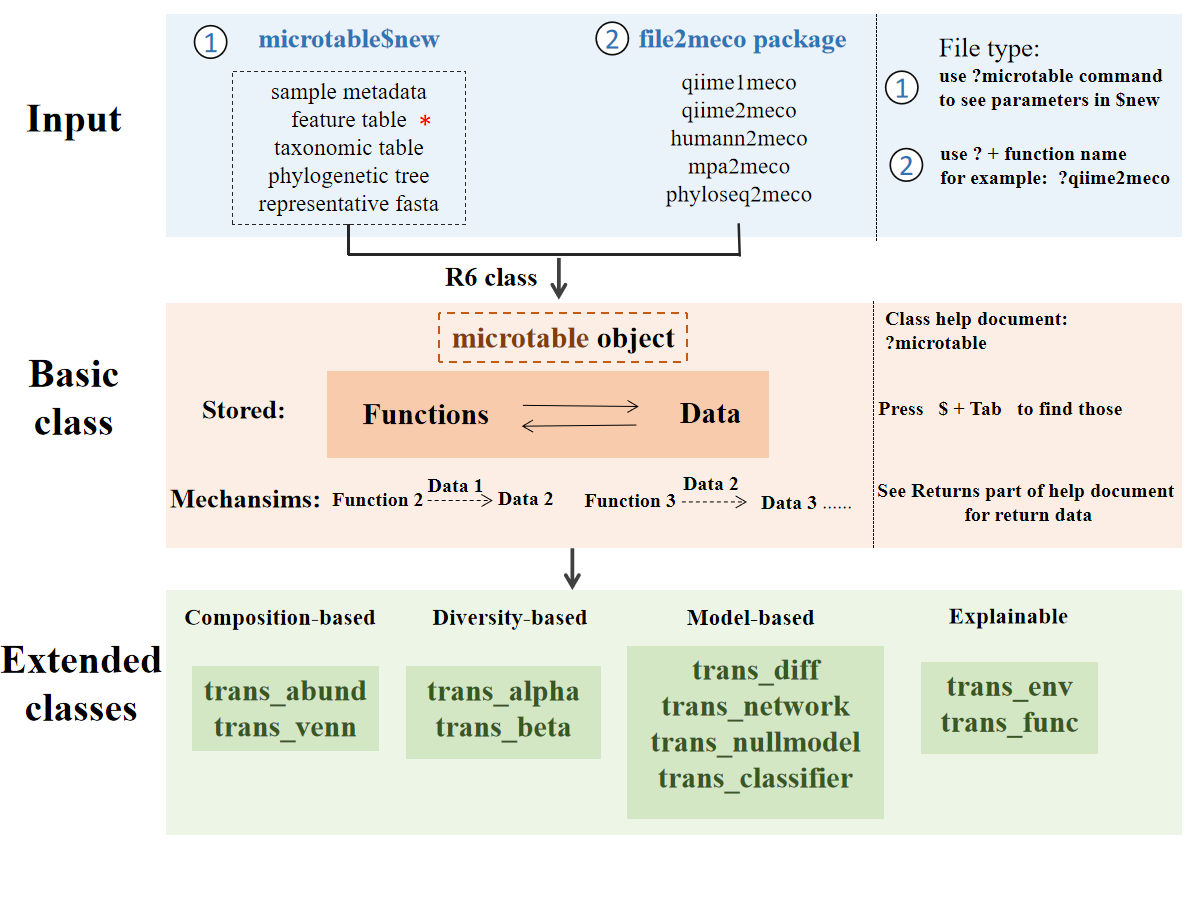
\includegraphics[width=800px]{Images/microeco_framework} \end{center}

The stored `Functions' and `Files' represent that the user can access those functions or files in R6 object using \$ operator
as shown in the figure. An example is the function \texttt{dataset\$cal\_alphadiv()} and its return result \texttt{dataset\$alpha\_diversity}.
The dataset is a microtable object.
Generally, the return files of functions are named with the prefix `res\_' to make users easily find them when using Rstudio and the keyboard shortcuts (Tab).
Except for microtable class, the transformed data in created object is generally named with the prefix `data\_'.

\hypertarget{r6-class}{%
\section{R6 Class}\label{r6-class}}

All the main classes in microeco package depend on the R6 class \citep{R6_Winston}.
R6 uses the encapsulated object-oriented (OO) programming paradigm,
which means that R6 is a profoundly different OO system from S3 and S4 because it is built on encapsulated objects, rather than generic functions.
If the user is interested in the class features, read more from `Advanced R' book (\url{https://adv-r.hadley.nz/}).

\begin{itemize}
\item
  A generic is a regular function, so it lives in the global namespace. An R6 method belongs to an object so it lives in a local namespace.
  This influences how we think about naming. The methods belong to objects, not generics, and the user can call them like object\$method().
\item
  R6's reference semantics allow methods to simultaneously return a value and modify an object.
\item
  Every R6 object has an S3 class that reflects its hierarchy of R6 class.
\end{itemize}

\hypertarget{help}{%
\section{Help}\label{help}}

The usage of help documents in the microeco package may be a little different from other packages we often used.
If the user wish to see the help document of a function, please search the name of the class it belongs to (not the name of the function)
and click the link of the function.

\begin{Shaded}
\begin{Highlighting}[]
\CommentTok{\# first install microeco, see https://github.com/ChiLiubio/microeco}
\CommentTok{\# load package microeco}
\FunctionTok{library}\NormalTok{(microeco)}
\end{Highlighting}
\end{Shaded}

\begin{Shaded}
\begin{Highlighting}[]
\CommentTok{\# show all the classes and tutorial links}
\NormalTok{?microeco}
\CommentTok{\# show the detailed description of the class microtable}
\CommentTok{\# same with: help(microtable)}
\NormalTok{?microtable}
\end{Highlighting}
\end{Shaded}

\hypertarget{rtools}{%
\section{RTools}\label{rtools}}

For Windows system, RTools (\url{https://cran.r-project.org/bin/windows/Rtools/}) is necessary to install some R packages from source, such as R packages deposited in GitHub.

\hypertarget{dependence}{%
\section{Dependence}\label{dependence}}

\hypertarget{description}{%
\subsection{Description}\label{description}}

To keep the start and use of microeco package simplified,
the installation of microeco only depend on several packages, which are compulsory-installed from CRAN and frequently used in the data analysis.
So the question is that the user may encounter an error when using a class or function that invoke an additional package like this:

\begin{Shaded}
\begin{Highlighting}[]
\FunctionTok{library}\NormalTok{(microeco)}
\FunctionTok{data}\NormalTok{(dataset)}
\NormalTok{test }\OtherTok{\textless{}{-}}\NormalTok{ trans\_network}\SpecialCharTok{$}\FunctionTok{new}\NormalTok{(}\AttributeTok{dataset =}\NormalTok{ dataset, }\AttributeTok{filter\_thres =} \FloatTok{0.001}\NormalTok{)}
\NormalTok{test}\SpecialCharTok{$}\FunctionTok{cal\_network}\NormalTok{(}\AttributeTok{network\_method =} \StringTok{"SpiecEasi"}\NormalTok{)}
\end{Highlighting}
\end{Shaded}

\begin{Shaded}
\begin{Highlighting}[]
\NormalTok{Error in test$cal\_network(network\_method = "SpiecEasi"): SpiecEasi package is not installed!}
\end{Highlighting}
\end{Shaded}

The reason is that network construction with `SpiecEasi' method requires SpiecEasi package to be installed.
This package is deposited in GitHub and can not be installed automatically.
In addition, we donot put some packages released in CRAN and Bioconductor on the ``Imports'' part of microeco package.

The solutions:

\begin{enumerate}
\def\labelenumi{\arabic{enumi}.}
\item
  Install the missing package when encounter such an error. Actually, it's very easy to install the packages from CRAN or Bioconductor or Github. Just have a try.
\item
  Install all the packages in advance.
  This is recommended if the user is interested in most of the methods and want to run a large number of examples in this tutorial.
  If so, please read all of the following sections and install these packages.
\end{enumerate}

\hypertarget{cran-packages}{%
\subsection{CRAN packages}\label{cran-packages}}

Some packages released in CRAN can not be installed automatically.
These packages are necessary to reproduce some parts of the tutorial.
If you want to install all of these packages or some of them, please run this:

\begin{Shaded}
\begin{Highlighting}[]
\CommentTok{\# allow more waiting time to download each package}
\FunctionTok{options}\NormalTok{(}\AttributeTok{timeout =} \DecValTok{1000}\NormalTok{)}
\CommentTok{\# If a package is not installed, it will be installed from CRAN}
\CommentTok{\# First select the packages of interest}
\NormalTok{tmp }\OtherTok{\textless{}{-}} \FunctionTok{c}\NormalTok{(}\StringTok{"microeco"}\NormalTok{, }\StringTok{"mecoturn"}\NormalTok{, }\StringTok{"MASS"}\NormalTok{, }\StringTok{"GUniFrac"}\NormalTok{, }\StringTok{"ggpubr"}\NormalTok{, }\StringTok{"randomForest"}\NormalTok{, }\StringTok{"ggdendro"}\NormalTok{, }\StringTok{"ggrepel"}\NormalTok{, }\StringTok{"agricolae"}\NormalTok{, }\StringTok{"igraph"}\NormalTok{, }\StringTok{"picante"}\NormalTok{, }\StringTok{"pheatmap"}\NormalTok{, }\StringTok{"rgexf"}\NormalTok{, }
    \StringTok{"ggalluvial"}\NormalTok{, }\StringTok{"ggh4x"}\NormalTok{, }\StringTok{"rcompanion"}\NormalTok{, }\StringTok{"FSA"}\NormalTok{, }\StringTok{"gridExtra"}\NormalTok{, }\StringTok{"aplot"}\NormalTok{, }\StringTok{"NST"}\NormalTok{, }\StringTok{"GGally"}\NormalTok{, }\StringTok{"ggraph"}\NormalTok{, }\StringTok{"networkD3"}\NormalTok{, }\StringTok{"poweRlaw"}\NormalTok{, }\StringTok{"ggtern"}\NormalTok{, }\StringTok{"SRS"}\NormalTok{)}
\CommentTok{\# Now check or install}
\ControlFlowTok{for}\NormalTok{(x }\ControlFlowTok{in}\NormalTok{ tmp)\{}
    \ControlFlowTok{if}\NormalTok{(}\SpecialCharTok{!}\FunctionTok{require}\NormalTok{(x, }\AttributeTok{character.only =} \ConstantTok{TRUE}\NormalTok{)) \{}
        \FunctionTok{install.packages}\NormalTok{(x, }\AttributeTok{dependencies =} \ConstantTok{TRUE}\NormalTok{)}
\NormalTok{    \}}
\NormalTok{\}}
\end{Highlighting}
\end{Shaded}

\hypertarget{bioconductor-packages}{%
\subsection{Bioconductor packages}\label{bioconductor-packages}}

Some dependent packages are deposited in bioconductor (\url{https://bioconductor.org}).
Please run the following commands to install them one by one.
Several packages may be installed from source.
So, for the Windows system, please make sure RTools has been installed (\url{https://chiliubio.github.io/microeco_tutorial/intro.html\#rtools}).

\begin{Shaded}
\begin{Highlighting}[]
\FunctionTok{install.packages}\NormalTok{(}\StringTok{"BiocManager"}\NormalTok{)}
\FunctionTok{install.packages}\NormalTok{(}\StringTok{"file2meco"}\NormalTok{, }\AttributeTok{repos =}\NormalTok{ BiocManager}\SpecialCharTok{::}\FunctionTok{repositories}\NormalTok{())}
\FunctionTok{install.packages}\NormalTok{(}\StringTok{"MicrobiomeStat"}\NormalTok{, }\AttributeTok{repos =}\NormalTok{ BiocManager}\SpecialCharTok{::}\FunctionTok{repositories}\NormalTok{())}
\FunctionTok{install.packages}\NormalTok{(}\StringTok{"WGCNA"}\NormalTok{, }\AttributeTok{repos =}\NormalTok{ BiocManager}\SpecialCharTok{::}\FunctionTok{repositories}\NormalTok{())}
\NormalTok{BiocManager}\SpecialCharTok{::}\FunctionTok{install}\NormalTok{(}\StringTok{"ggtree"}\NormalTok{)}
\NormalTok{BiocManager}\SpecialCharTok{::}\FunctionTok{install}\NormalTok{(}\StringTok{"metagenomeSeq"}\NormalTok{)}
\NormalTok{BiocManager}\SpecialCharTok{::}\FunctionTok{install}\NormalTok{(}\StringTok{"ALDEx2"}\NormalTok{)}
\NormalTok{BiocManager}\SpecialCharTok{::}\FunctionTok{install}\NormalTok{(}\StringTok{"ANCOMBC"}\NormalTok{)}
\end{Highlighting}
\end{Shaded}

\hypertarget{github-packages}{%
\subsection{Github packages}\label{github-packages}}

A part of dependent packages in some methods comes from Github (\url{https://github.com/}).
Each package from the GitHub platform is accompanied by installation instructions.
However, due to the network instability of the platform, certain packages may fail to install online.
As a result, in order to facilitate quick and convenient installation,
we have collected these GitHub-dependent packages and consolidated them within a dedicated project repository (\url{https://github.com/ChiLiubio/microeco_dependence}).
Please run the following commands to install them.
For the Windows system, first make sure RTools has been installed (\url{https://chiliubio.github.io/microeco_tutorial/intro.html\#rtools}).

\begin{Shaded}
\begin{Highlighting}[]
\CommentTok{\# downloading link of the compressed archive}
\NormalTok{url }\OtherTok{\textless{}{-}} \StringTok{"https://github.com/ChiLiubio/microeco\_dependence/releases/download/v0.20.0/microeco\_dependence.zip"}
\CommentTok{\# allow more time to download the zip file in R}
\FunctionTok{options}\NormalTok{(}\AttributeTok{timeout =} \DecValTok{2000}\NormalTok{)}
\CommentTok{\# If failed or too slow, please open the upper url in browser or other tool to download the zip file and move it to the current R working directory}
\FunctionTok{download.file}\NormalTok{(}\AttributeTok{url =}\NormalTok{ url, }\AttributeTok{destfile =} \StringTok{"microeco\_dependence.zip"}\NormalTok{)}
\CommentTok{\# uncompress the file in R}
\NormalTok{tmp }\OtherTok{\textless{}{-}} \StringTok{"microeco\_dependence"}
\FunctionTok{unzip}\NormalTok{(}\FunctionTok{paste0}\NormalTok{(tmp, }\StringTok{".zip"}\NormalTok{))}
\CommentTok{\# install devtools}
\ControlFlowTok{if}\NormalTok{(}\SpecialCharTok{!}\FunctionTok{require}\NormalTok{(}\StringTok{"devtools"}\NormalTok{, }\AttributeTok{character.only =} \ConstantTok{TRUE}\NormalTok{))\{}\FunctionTok{install.packages}\NormalTok{(}\StringTok{"devtools"}\NormalTok{, }\AttributeTok{dependencies =} \ConstantTok{TRUE}\NormalTok{)\}}
\CommentTok{\# run these one by one}
\NormalTok{devtools}\SpecialCharTok{::}\FunctionTok{install\_local}\NormalTok{(}\FunctionTok{paste0}\NormalTok{(tmp, }\StringTok{"/"}\NormalTok{, }\StringTok{"SpiecEasi{-}master.zip"}\NormalTok{), }\AttributeTok{dependencies =} \ConstantTok{TRUE}\NormalTok{)}
\NormalTok{devtools}\SpecialCharTok{::}\FunctionTok{install\_local}\NormalTok{(}\FunctionTok{paste0}\NormalTok{(tmp, }\StringTok{"/"}\NormalTok{, }\StringTok{"mixedCCA{-}master.zip"}\NormalTok{), }\AttributeTok{dependencies =} \ConstantTok{TRUE}\NormalTok{)}
\NormalTok{devtools}\SpecialCharTok{::}\FunctionTok{install\_local}\NormalTok{(}\FunctionTok{paste0}\NormalTok{(tmp, }\StringTok{"/"}\NormalTok{, }\StringTok{"SPRING{-}master.zip"}\NormalTok{), }\AttributeTok{dependencies =} \ConstantTok{TRUE}\NormalTok{)}
\NormalTok{devtools}\SpecialCharTok{::}\FunctionTok{install\_local}\NormalTok{(}\FunctionTok{paste0}\NormalTok{(tmp, }\StringTok{"/"}\NormalTok{, }\StringTok{"NetCoMi{-}main.zip"}\NormalTok{), }\AttributeTok{repos =}\NormalTok{ BiocManager}\SpecialCharTok{::}\FunctionTok{repositories}\NormalTok{())}
\NormalTok{devtools}\SpecialCharTok{::}\FunctionTok{install\_local}\NormalTok{(}\FunctionTok{paste0}\NormalTok{(tmp, }\StringTok{"/"}\NormalTok{, }\StringTok{"beem{-}static{-}master.zip"}\NormalTok{), }\AttributeTok{dependencies =} \ConstantTok{TRUE}\NormalTok{)}
\NormalTok{devtools}\SpecialCharTok{::}\FunctionTok{install\_local}\NormalTok{(}\FunctionTok{paste0}\NormalTok{(tmp, }\StringTok{"/"}\NormalTok{, }\StringTok{"chorddiag{-}master.zip"}\NormalTok{), }\AttributeTok{dependencies =} \ConstantTok{TRUE}\NormalTok{)}
\NormalTok{devtools}\SpecialCharTok{::}\FunctionTok{install\_local}\NormalTok{(}\FunctionTok{paste0}\NormalTok{(tmp, }\StringTok{"/"}\NormalTok{, }\StringTok{"ggradar{-}master.zip"}\NormalTok{), }\AttributeTok{dependencies =} \ConstantTok{TRUE}\NormalTok{)}
\NormalTok{devtools}\SpecialCharTok{::}\FunctionTok{install\_local}\NormalTok{(}\FunctionTok{paste0}\NormalTok{(tmp, }\StringTok{"/"}\NormalTok{, }\StringTok{"ggnested{-}main.zip"}\NormalTok{), }\AttributeTok{dependencies =} \ConstantTok{TRUE}\NormalTok{)}
\NormalTok{devtools}\SpecialCharTok{::}\FunctionTok{install\_local}\NormalTok{(}\FunctionTok{paste0}\NormalTok{(tmp, }\StringTok{"/"}\NormalTok{, }\StringTok{"ggcor{-}1{-}master.zip"}\NormalTok{), }\AttributeTok{dependencies =} \ConstantTok{TRUE}\NormalTok{)}
\end{Highlighting}
\end{Shaded}

\hypertarget{gephi}{%
\subsection{Gephi}\label{gephi}}

Gephi is an excellent network visualization tool and used to open the saved network file,
i.e.~network.gexf in the \href{https://chiliubio.github.io/microeco_tutorial/model-based-class.html\#trans_network-class}{tutorial}.
You can download Gephi and learn how to use it from \url{https://gephi.org/users/download/}

\hypertarget{tax4fun}{%
\subsection{Tax4Fun}\label{tax4fun}}

Tax4Fun is an R package used for predicting the functional potential of prokaryotic communities.

\begin{enumerate}
\def\labelenumi{\arabic{enumi}.}
\tightlist
\item
  install Tax4Fun package
\end{enumerate}

\begin{Shaded}
\begin{Highlighting}[]
\FunctionTok{install.packages}\NormalTok{(}\StringTok{"RJSONIO"}\NormalTok{)}
\FunctionTok{install.packages}\NormalTok{(}\FunctionTok{system.file}\NormalTok{(}\StringTok{"extdata"}\NormalTok{, }\StringTok{"biom\_0.3.12.tar.gz"}\NormalTok{, }\AttributeTok{package=}\StringTok{"microeco"}\NormalTok{), }\AttributeTok{repos =} \ConstantTok{NULL}\NormalTok{, }\AttributeTok{type =} \StringTok{"source"}\NormalTok{)}
\FunctionTok{install.packages}\NormalTok{(}\FunctionTok{system.file}\NormalTok{(}\StringTok{"extdata"}\NormalTok{, }\StringTok{"qiimer\_0.9.4.tar.gz"}\NormalTok{, }\AttributeTok{package=}\StringTok{"microeco"}\NormalTok{), }\AttributeTok{repos =} \ConstantTok{NULL}\NormalTok{, }\AttributeTok{type =} \StringTok{"source"}\NormalTok{)}
\FunctionTok{install.packages}\NormalTok{(}\FunctionTok{system.file}\NormalTok{(}\StringTok{"extdata"}\NormalTok{, }\StringTok{"Tax4Fun\_0.3.1.tar.gz"}\NormalTok{, }\AttributeTok{package=}\StringTok{"microeco"}\NormalTok{), }\AttributeTok{repos =} \ConstantTok{NULL}\NormalTok{, }\AttributeTok{type =} \StringTok{"source"}\NormalTok{)}
\end{Highlighting}
\end{Shaded}

\begin{enumerate}
\def\labelenumi{\arabic{enumi}.}
\setcounter{enumi}{1}
\tightlist
\item
  download SILVA123 reference data from \url{http://tax4fun.gobics.de/}\\
   unzip SILVA123.zip and provide this path to the folderReferenceData parameter of cal\_tax4fun function in trans\_func class.
\end{enumerate}

\hypertarget{tax4fun2}{%
\subsection{Tax4Fun2}\label{tax4fun2}}

Tax4Fun2 is another R package for the the prediction of functional profiles and functional gene redundancies of prokaryotic communities \citep{Wemheuer_Tax4Fun2_2020}.
It has higher accuracies than PICRUSt and Tax4Fun. The Tax4Fun2 approach implemented in microeco is a little different from the original package.
Using Tax4Fun2 approach require the representative fasta file.
The user do not need to install Tax4Fun2 R package again.
The only thing need to do is to download the blast tool (\textbf{ignore this if the blast tool has been in the path}) and Ref99NR/Ref100NR database (select one).
Download blast tools from ``\url{https://ftp.ncbi.nlm.nih.gov/blast/executables/blast+}'' ; e.g.~ncbi-blast-****-x64-win64.tar.gz for windows system.
Note that some errors can come from the latest versions because of memory issue (\url{https://www.biostars.org/p/413294/}).
An easy solution is to use previous version (such as 2.5.0).
Download Ref99NR.zip from ``\url{https://cloudstor.aarnet.edu.au/plus/s/DkoZIyZpMNbrzSw/download}'' or Ref100NR.zip from ``\url{https://cloudstor.aarnet.edu.au/plus/s/jIByczak9ZAFUB4/download}'' .
Uncompress all the folders. The final folders should be like these structures:

blast tools:\\
 \textbar-- ncbi-blast-2.5.0+\\
  \textbar---- bin\\
   \textbar------ blastn.exe\\
   \textbar------ makeblastdb.exe\\
   \textbar------ \ldots\ldots{}

Ref99NR:\\
 \textbar-- Tax4Fun2\_ReferenceData\_v2\\
  \textbar---- Ref99NR\\
   \textbar------ otu000001.tbl.gz\\
   \textbar------ \ldots\ldots{}\\
   \textbar------ Ref99NR.fasta\\
   \textbar------ Ref99NR.tre

The path ``Tax4Fun2\_ReferenceData\_v2'' will be required in the trans\_func\$cal\_tax4fun2() function.
The blast tool path ``ncbi-blast-2.5.0+/bin'' is also required if it is not added to the system env path (environmental variable).

\begin{Shaded}
\begin{Highlighting}[]
\CommentTok{\# Either seqinr or Biostrings package should be installed for reading and writing fasta file}
\FunctionTok{install.packages}\NormalTok{(}\StringTok{"seqinr"}\NormalTok{, }\AttributeTok{dependencies =} \ConstantTok{TRUE}\NormalTok{)}
\CommentTok{\# or install Biostrings from bioconductor https://bioconductor.org/packages/release/bioc/html/Biostrings.html}
\CommentTok{\# Now we show how to read the fasta file}
\CommentTok{\# see https://github.com/ChiLiubio/file2meco to install file2meco}
\NormalTok{rep\_fasta\_path }\OtherTok{\textless{}{-}} \FunctionTok{system.file}\NormalTok{(}\StringTok{"extdata"}\NormalTok{, }\StringTok{"rep.fna"}\NormalTok{, }\AttributeTok{package=}\StringTok{"file2meco"}\NormalTok{)}
\NormalTok{rep\_fasta }\OtherTok{\textless{}{-}}\NormalTok{ seqinr}\SpecialCharTok{::}\FunctionTok{read.fasta}\NormalTok{(rep\_fasta\_path)}
\CommentTok{\# or use Biostrings package}
\NormalTok{rep\_fasta }\OtherTok{\textless{}{-}}\NormalTok{ Biostrings}\SpecialCharTok{::}\FunctionTok{readDNAStringSet}\NormalTok{(rep\_fasta\_path)}
\CommentTok{\# try to create a microtable object with rep\_fasta}
\FunctionTok{data}\NormalTok{(}\StringTok{"otu\_table\_16S"}\NormalTok{)}
\CommentTok{\# In microtable class, all the taxa names should be necessarily included in rep\_fasta}
\NormalTok{otu\_table\_16S }\OtherTok{\textless{}{-}}\NormalTok{ otu\_table\_16S[}\FunctionTok{rownames}\NormalTok{(otu\_table\_16S) }\SpecialCharTok{\%in\%} \FunctionTok{names}\NormalTok{(rep\_fasta), ]}
\NormalTok{test }\OtherTok{\textless{}{-}}\NormalTok{ microtable}\SpecialCharTok{$}\FunctionTok{new}\NormalTok{(}\AttributeTok{otu\_table =}\NormalTok{ otu\_table\_16S, }\AttributeTok{rep\_fasta =}\NormalTok{ rep\_fasta)}
\NormalTok{test}
\end{Highlighting}
\end{Shaded}

\hypertarget{plot}{%
\section{Plot}\label{plot}}

Most of the plots in the package rely on the ggplot2 package system.
We provide some parameters to optimize the corresponding plot, but it may be far from enough.
The user can also assign the output a name and use the ggplot2-style grammers to modify it.
Each data table used for visualization is stored in the object and can be saved for the customized analysis.
Of course, the user can also directly modify the class and reload them to use.
Any contribution of a modified class is appreciated via Github-Pull requests (\url{https://github.com/ChiLiubio/microeco_tutorial/pulls}) or Email (\href{mailto:liuchi0426@126.com}{\nolinkurl{liuchi0426@126.com}}).

\hypertarget{rstudio}{%
\section{Rstudio}\label{rstudio}}

The modular design of help documentation can facilitate the document viewing.
However, in Rtudio, there may be instances where the links fail to navigate properly.
In such cases, the issue can be resolved by reopening a document window, as illustrated in the figure below.

\begin{center}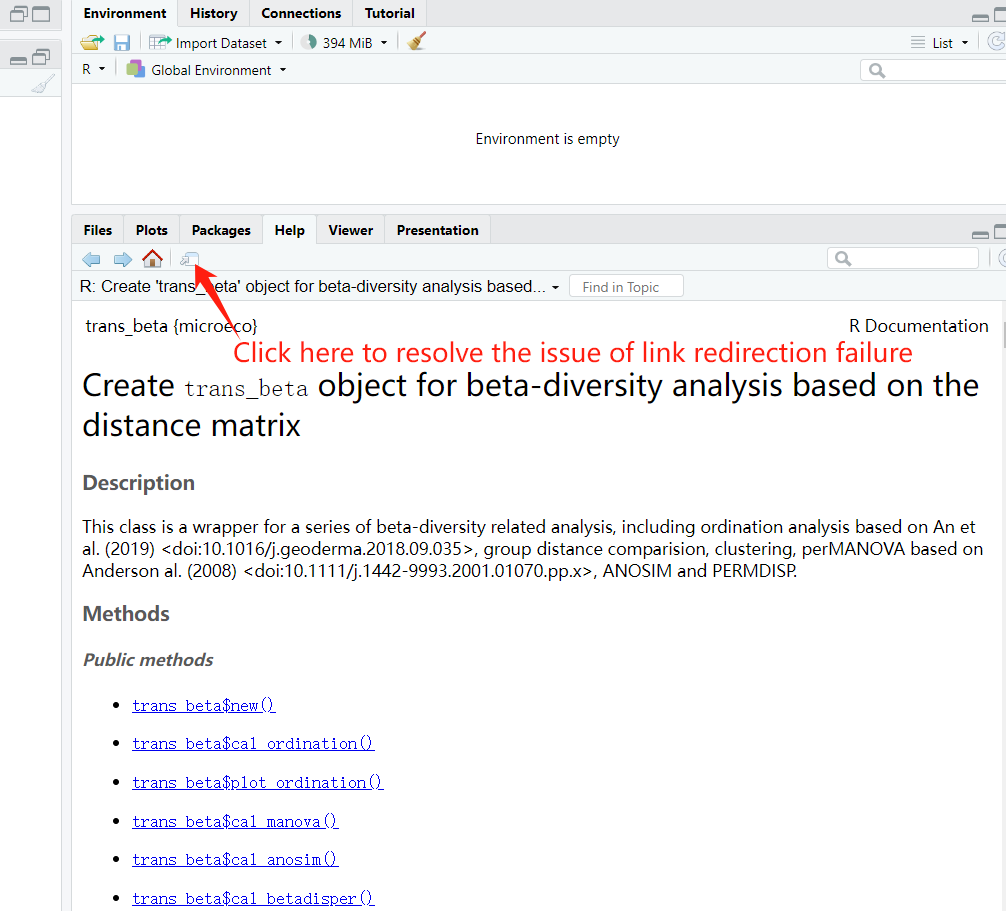
\includegraphics[width=800px]{Images/Rstudio_link_redirection} \end{center}

\hypertarget{basic-class}{%
\chapter{Basic class}\label{basic-class}}

The microtable class is the basic class.
All the other classes depend on the microtable class.

\begin{center}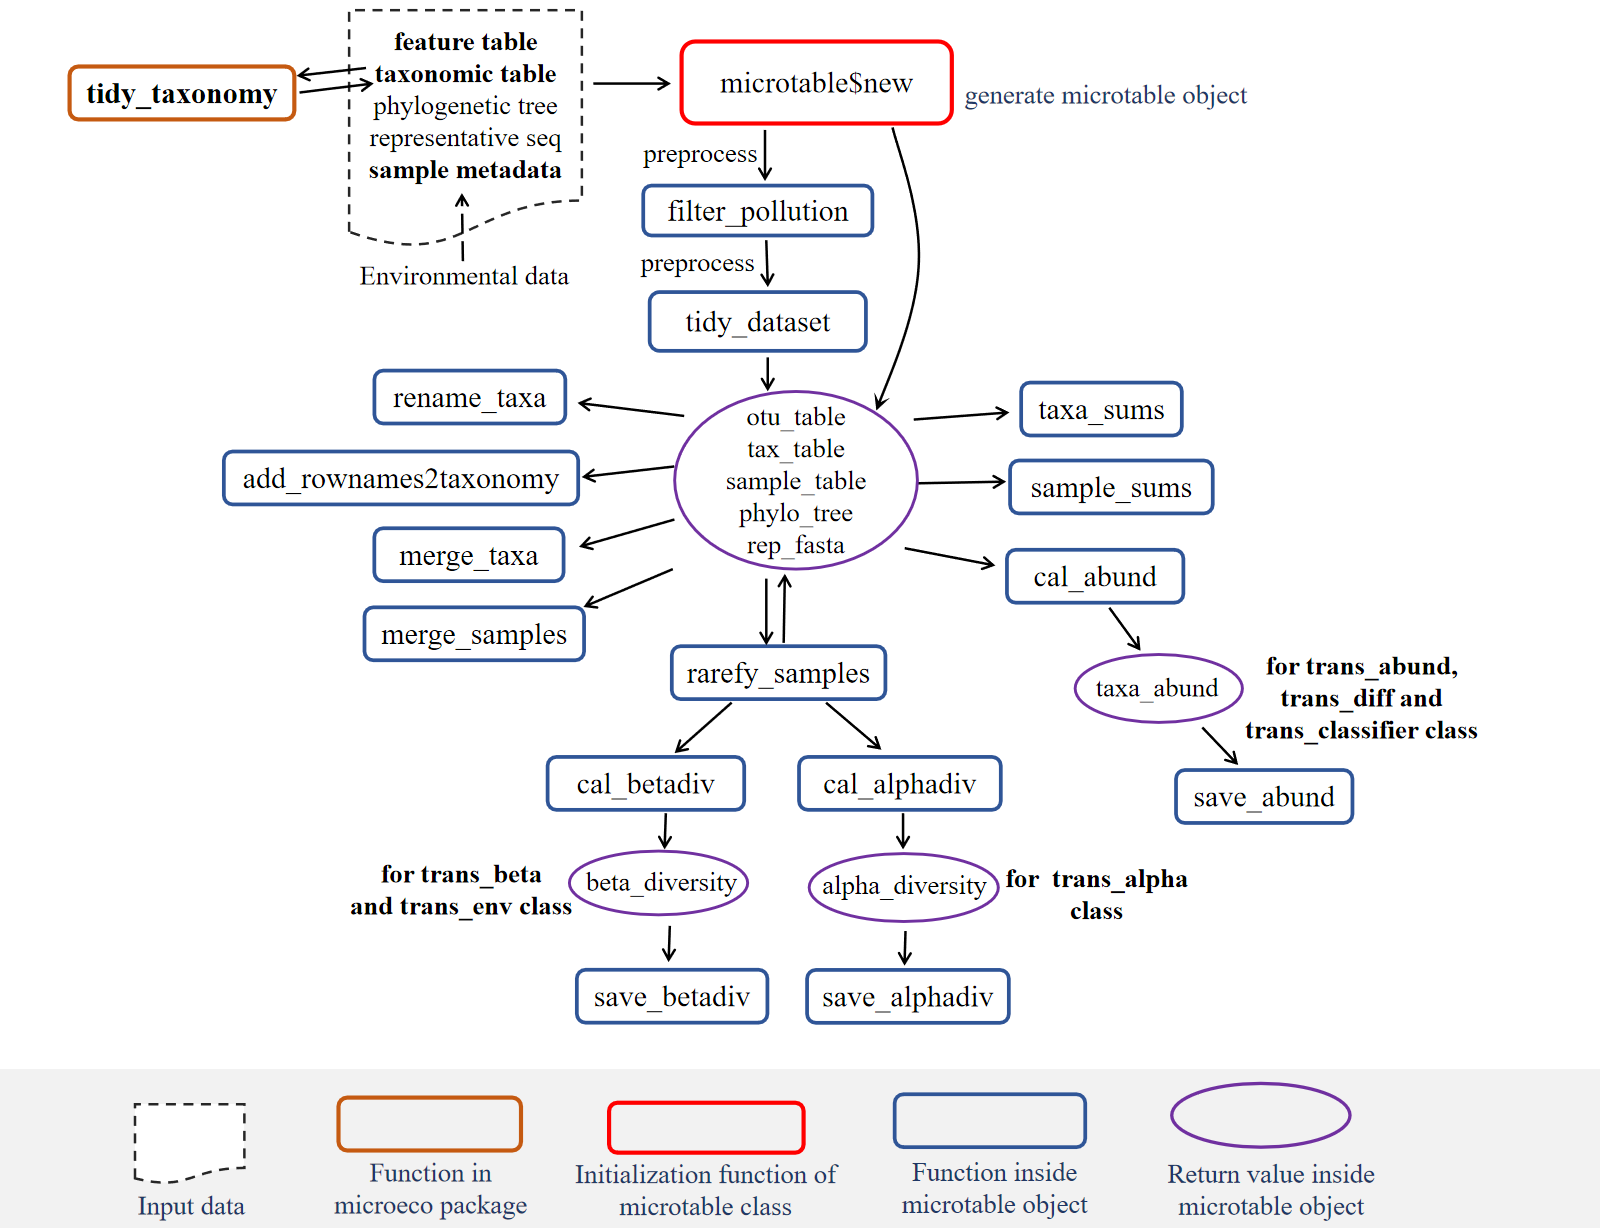
\includegraphics[width=8000px]{Images/microtable_framework} \end{center}

The objects inside the rectangle with full line represent functions.
The red rectangle means it is extremely important function.
The dashed line denotes the key objects (input or output of functions) that deserve more attention.

\hypertarget{microtable-class}{%
\section{microtable class}\label{microtable-class}}

 Many tools can be used for the bioinformatic analysis of amplicon sequencing data, such as QIIME \citep{Caporaso_QIIME_2010}, QIIME2 \citep{Bolyen_Reproducible_2019},
usearch (\url{https://www.drive5.com/usearch/}), mothur \citep{Schloss_Introducing_2009},
SILVAngs (\url{https://ngs.arb-silva.de/silvangs/}), LotuS2 \citep{Ozkurt_LotuS2_2022},
and RDP (\url{http://rdp.cme.msu.edu/}).
Although the formats of result files may vary across tools, the main contents can be generally classified into the following parts:
(1) OTU/ASV table, i.e.~the feature-sample abundance table;
(2) taxonomic assignment table;
(3) representative sequences;
(4) phylogenetic tree;
(5) metadata.
It is generally useful to create a detailed sample metadata table to store all the sample information (including the environmental data).

 The microtable class is the basic class and designed to store the basic data for all the downstream analysis in the microeco package.
At least, the OTU table (i.e.~feature-sample abundance table) should be provided to create microtable object.
Thus, the microtable class can determine that the sample information table is missing and create a default sample table according to
sample names in otu\_table.
To make the file input more convenient,
we also build another R package file2meco (\url{https://github.com/ChiLiubio/file2meco}) to read the output files of some tools into microtable object.
Currently, those tools/softwares include not only commonly-used QIIME \citep{Caporaso_QIIME_2010} and QIIME2\citep{Bolyen_Reproducible_2019},
but also several metagenomic tools, such as HUMAnN \citep{Franzosa_Species_2018} and kraken2 \citep{Wood_Improved_2019}.
In this tutorial, the data inside the package was employed to show some basic operations.

\hypertarget{prepare-the-example-data}{%
\subsection{Prepare the example data}\label{prepare-the-example-data}}

 The example data inside the microeco package is used to show the main part of the tutorial.
This dataset arose from 16S rRNA gene Miseq sequencing results of wetland soils in China published by An et al. \citep{An_Soil_2019},
who surveyed soil prokaryotic communities in Chinese inland wetlands (IW),
coastal wetland (CW) and Tibet plateau wetlands (TW) using amplicon sequencing.
These wetlands include both saline and non-saline samples (classified for the tutorial).
The sample information table has 4 columns: ``SampleID'', ``Group'', ``Type'' and ``Saline''.
The column ``SampleID'' is same with the rownames.
The column ``Group'' represents the IW, CW and TW.
The column ``Type'' means the sampling region: northeastern region (NE), northwest region (NW), North China area (NC),
middle-lower reaches of the Yangtze River (YML), southern coastal area (SC), upper reaches of the Yangtze River (YU), Qinghai-Tibet Plateau (QTP).
The column ``Saline'' denotes the saline soils and non-saline soils.
In this dataset, the environmental factor table is separated from the sample information table.
It is also recommended to put all the environmental data into sample information table.

\begin{Shaded}
\begin{Highlighting}[]
\FunctionTok{library}\NormalTok{(microeco)}
\CommentTok{\# load the example data; 16S rRNA gene amplicon sequencing dataset}
\CommentTok{\# metadata table; data.frame}
\FunctionTok{data}\NormalTok{(sample\_info\_16S)}
\CommentTok{\# feature table; data.frame}
\FunctionTok{data}\NormalTok{(otu\_table\_16S)}
\CommentTok{\# taxonomic assignment table; data.frame}
\FunctionTok{data}\NormalTok{(taxonomy\_table\_16S)}
\CommentTok{\# phylogenetic tree; not necessary; use for the phylogenetic analysis}
\CommentTok{\# Newick format; use read.tree function of ape package to read a tree}
\FunctionTok{data}\NormalTok{(phylo\_tree\_16S)}
\CommentTok{\# load the environmental data table if it is not in sample table}
\FunctionTok{data}\NormalTok{(env\_data\_16S)}
\CommentTok{\# use pipe operator in magrittr package}
\FunctionTok{library}\NormalTok{(magrittr)}
\CommentTok{\# fix the random number generation to make the results repeatable}
\FunctionTok{set.seed}\NormalTok{(}\DecValTok{123}\NormalTok{)}
\CommentTok{\# make the plotting background same with the tutorial}
\FunctionTok{library}\NormalTok{(ggplot2)}
\FunctionTok{theme\_set}\NormalTok{(}\FunctionTok{theme\_bw}\NormalTok{())}
\end{Highlighting}
\end{Shaded}

Make sure that the data types of sample\_table, otu\_table and tax\_table are all \texttt{data.frame} format as the following part shows.

\begin{Shaded}
\begin{Highlighting}[]
\FunctionTok{class}\NormalTok{(otu\_table\_16S)}
\end{Highlighting}
\end{Shaded}

\begin{verbatim}
## [1] "data.frame"
\end{verbatim}

\begin{Shaded}
\begin{Highlighting}[]
\NormalTok{otu\_table\_16S[}\DecValTok{1}\SpecialCharTok{:}\DecValTok{5}\NormalTok{, }\DecValTok{1}\SpecialCharTok{:}\DecValTok{5}\NormalTok{]}
\end{Highlighting}
\end{Shaded}

\begin{longtable}[]{@{}
  >{\centering\arraybackslash}p{(\columnwidth - 10\tabcolsep) * \real{0.2083}}
  >{\centering\arraybackslash}p{(\columnwidth - 10\tabcolsep) * \real{0.0694}}
  >{\centering\arraybackslash}p{(\columnwidth - 10\tabcolsep) * \real{0.0694}}
  >{\centering\arraybackslash}p{(\columnwidth - 10\tabcolsep) * \real{0.0694}}
  >{\centering\arraybackslash}p{(\columnwidth - 10\tabcolsep) * \real{0.0694}}
  >{\centering\arraybackslash}p{(\columnwidth - 10\tabcolsep) * \real{0.0833}}@{}}
\toprule()
\begin{minipage}[b]{\linewidth}\centering
~
\end{minipage} & \begin{minipage}[b]{\linewidth}\centering
S1
\end{minipage} & \begin{minipage}[b]{\linewidth}\centering
S2
\end{minipage} & \begin{minipage}[b]{\linewidth}\centering
S3
\end{minipage} & \begin{minipage}[b]{\linewidth}\centering
S4
\end{minipage} & \begin{minipage}[b]{\linewidth}\centering
S5
\end{minipage} \\
\midrule()
\endhead
\textbf{OTU\_4272} & 1 & 0 & 1 & 1 & 0 \\
\textbf{OTU\_236} & 1 & 4 & 0 & 2 & 35 \\
\textbf{OTU\_399} & 9 & 2 & 2 & 4 & 4 \\
\textbf{OTU\_1556} & 5 & 18 & 7 & 3 & 2 \\
\textbf{OTU\_32} & 83 & 9 & 19 & 8 & 102 \\
\bottomrule()
\end{longtable}

\begin{Shaded}
\begin{Highlighting}[]
\FunctionTok{class}\NormalTok{(taxonomy\_table\_16S)}
\end{Highlighting}
\end{Shaded}

\begin{verbatim}
## [1] "data.frame"
\end{verbatim}

\begin{Shaded}
\begin{Highlighting}[]
\NormalTok{taxonomy\_table\_16S[}\DecValTok{1}\SpecialCharTok{:}\DecValTok{5}\NormalTok{, }\DecValTok{1}\SpecialCharTok{:}\DecValTok{3}\NormalTok{]}
\end{Highlighting}
\end{Shaded}

\begin{longtable}[]{@{}
  >{\centering\arraybackslash}p{(\columnwidth - 6\tabcolsep) * \real{0.1974}}
  >{\centering\arraybackslash}p{(\columnwidth - 6\tabcolsep) * \real{0.1842}}
  >{\centering\arraybackslash}p{(\columnwidth - 6\tabcolsep) * \real{0.3026}}
  >{\centering\arraybackslash}p{(\columnwidth - 6\tabcolsep) * \real{0.3158}}@{}}
\toprule()
\begin{minipage}[b]{\linewidth}\centering
~
\end{minipage} & \begin{minipage}[b]{\linewidth}\centering
Kingdom
\end{minipage} & \begin{minipage}[b]{\linewidth}\centering
Phylum
\end{minipage} & \begin{minipage}[b]{\linewidth}\centering
Class
\end{minipage} \\
\midrule()
\endhead
\textbf{OTU\_4272} & k\_\_Bacteria & p\_\_Firmicutes & c\_\_Bacilli \\
\textbf{OTU\_236} & k\_\_Bacteria & p\_\_Chloroflexi & c\_\_ \\
\textbf{OTU\_399} & k\_\_Bacteria & p\_\_Proteobacteria & c\_\_Betaproteobacteria \\
\textbf{OTU\_1556} & k\_\_Bacteria & p\_\_Acidobacteria & c\_\_Acidobacteria \\
\textbf{OTU\_32} & k\_\_Archaea & p\_\_Miscellaneous
Crenarchaeotic Group & c\_\_ \\
\bottomrule()
\end{longtable}

Generally, users' taxonomic table has some messy information, such as NA, unidentified and unknown.
These information can potentially influence the following taxonomic abundance calculation and other taxonomy-based analysis.
So it is usually necessary to clean this data using the \texttt{tidy\_taxonomy} function.
Another very important result of this operation is to \textbf{unify the taxonomic prefix} automatically,
e.g., converting D\_1\_\_ to p\_\_ for Phylum level or adding p\_\_ to Phylum directly if no prefix is found.

\begin{Shaded}
\begin{Highlighting}[]
\CommentTok{\# make the taxonomic information unified, very important}
\NormalTok{taxonomy\_table\_16S }\SpecialCharTok{\%\textless{}\textgreater{}\%}\NormalTok{ tidy\_taxonomy}
\end{Highlighting}
\end{Shaded}

The rownames of sample\_table in microtable object (i.e.~sample names) are used for selecting samples/groups in all the related operations in the package.
Using pure number as sample names is \textbf{not recommended} in case of unknown disorder or man-made mistake.
\textbf{Before creating microtable object, make sure that the rownames of sample information table are sample names}.

\begin{Shaded}
\begin{Highlighting}[]
\FunctionTok{class}\NormalTok{(sample\_info\_16S)}
\end{Highlighting}
\end{Shaded}

\begin{verbatim}
## [1] "data.frame"
\end{verbatim}

\begin{Shaded}
\begin{Highlighting}[]
\NormalTok{sample\_info\_16S[}\DecValTok{1}\SpecialCharTok{:}\DecValTok{5}\NormalTok{, ]}
\end{Highlighting}
\end{Shaded}

\begin{longtable}[]{@{}
  >{\centering\arraybackslash}p{(\columnwidth - 8\tabcolsep) * \real{0.1250}}
  >{\centering\arraybackslash}p{(\columnwidth - 8\tabcolsep) * \real{0.1528}}
  >{\centering\arraybackslash}p{(\columnwidth - 8\tabcolsep) * \real{0.1111}}
  >{\centering\arraybackslash}p{(\columnwidth - 8\tabcolsep) * \real{0.0972}}
  >{\centering\arraybackslash}p{(\columnwidth - 8\tabcolsep) * \real{0.2500}}@{}}
\toprule()
\begin{minipage}[b]{\linewidth}\centering
~
\end{minipage} & \begin{minipage}[b]{\linewidth}\centering
SampleID
\end{minipage} & \begin{minipage}[b]{\linewidth}\centering
Group
\end{minipage} & \begin{minipage}[b]{\linewidth}\centering
Type
\end{minipage} & \begin{minipage}[b]{\linewidth}\centering
Saline
\end{minipage} \\
\midrule()
\endhead
\textbf{S1} & S1 & IW & NE & Non-saline soil \\
\textbf{S2} & S2 & IW & NE & Non-saline soil \\
\textbf{S3} & S3 & IW & NE & Non-saline soil \\
\textbf{S4} & S4 & IW & NE & Non-saline soil \\
\textbf{S5} & S5 & IW & NE & Non-saline soil \\
\bottomrule()
\end{longtable}

In this example, the environmental data is stored in the env\_data\_16S alone.
The user can also directly integrate those data into the sample information table.

\begin{Shaded}
\begin{Highlighting}[]
\FunctionTok{class}\NormalTok{(env\_data\_16S)}
\end{Highlighting}
\end{Shaded}

\begin{verbatim}
## [1] "data.frame"
\end{verbatim}

\begin{longtable}[]{@{}
  >{\centering\arraybackslash}p{(\columnwidth - 10\tabcolsep) * \real{0.1233}}
  >{\centering\arraybackslash}p{(\columnwidth - 10\tabcolsep) * \real{0.1507}}
  >{\centering\arraybackslash}p{(\columnwidth - 10\tabcolsep) * \real{0.1644}}
  >{\centering\arraybackslash}p{(\columnwidth - 10\tabcolsep) * \real{0.1507}}
  >{\centering\arraybackslash}p{(\columnwidth - 10\tabcolsep) * \real{0.1918}}
  >{\centering\arraybackslash}p{(\columnwidth - 10\tabcolsep) * \real{0.2192}}@{}}
\toprule()
\begin{minipage}[b]{\linewidth}\centering
~
\end{minipage} & \begin{minipage}[b]{\linewidth}\centering
Latitude
\end{minipage} & \begin{minipage}[b]{\linewidth}\centering
Longitude
\end{minipage} & \begin{minipage}[b]{\linewidth}\centering
Altitude
\end{minipage} & \begin{minipage}[b]{\linewidth}\centering
Temperature
\end{minipage} & \begin{minipage}[b]{\linewidth}\centering
Precipitation
\end{minipage} \\
\midrule()
\endhead
\textbf{S1} & 52.96 & 122.6 & 432 & -4.2 & 445 \\
\textbf{S2} & 52.95 & 122.6 & 445 & -4.3 & 449 \\
\textbf{S3} & 52.95 & 122.6 & 430 & -4.3 & 449 \\
\textbf{S4} & 52.95 & 122.6 & 430 & -4.3 & 449 \\
\textbf{S5} & 52.95 & 122.6 & 429 & -4.3 & 449 \\
\bottomrule()
\end{longtable}

\begin{Shaded}
\begin{Highlighting}[]
\FunctionTok{class}\NormalTok{(phylo\_tree\_16S)}
\end{Highlighting}
\end{Shaded}

\begin{verbatim}
## [1] "phylo"
\end{verbatim}

Then, we create an object of microtable class.
This operation is very similar with the package phyloseq\citep{Mcmurdie_phyloseq_2013}, but in microeco it is more brief.
The otu\_table in the microtable class must be the feature-sample format: rownames - OTU/ASV/pathway/other names; colnames - sample names.
\textbf{The colnames in otu\_table must have overlap with rownames of sample\_table}.
Otherwise, the following check can filter all the samples of otu\_table because of no same sample names between otu\_table and sample\_table.

\begin{Shaded}
\begin{Highlighting}[]
\CommentTok{\# In R6 class, \textquotesingle{}$new\textquotesingle{} is the original method used to create a new object of class}
\CommentTok{\# If you only provide abundance table, the class can help you create a sample info table}
\NormalTok{dataset }\OtherTok{\textless{}{-}}\NormalTok{ microtable}\SpecialCharTok{$}\FunctionTok{new}\NormalTok{(}\AttributeTok{otu\_table =}\NormalTok{ otu\_table\_16S)}
\end{Highlighting}
\end{Shaded}

\begin{verbatim}
## No sample_table provided, automatically use colnames in otu_table to create one ...
\end{verbatim}

\begin{Shaded}
\begin{Highlighting}[]
\FunctionTok{class}\NormalTok{(dataset)}
\end{Highlighting}
\end{Shaded}

\begin{verbatim}
## [1] "microtable" "R6"
\end{verbatim}

\begin{Shaded}
\begin{Highlighting}[]
\CommentTok{\# generally add the metadata}
\NormalTok{dataset }\OtherTok{\textless{}{-}}\NormalTok{ microtable}\SpecialCharTok{$}\FunctionTok{new}\NormalTok{(}\AttributeTok{otu\_table =}\NormalTok{ otu\_table\_16S, }\AttributeTok{sample\_table =}\NormalTok{ sample\_info\_16S)}
\NormalTok{dataset}
\end{Highlighting}
\end{Shaded}

\begin{verbatim}
## microtable-class object:
## sample_table have 90 rows and 4 columns
## otu_table have 13628 rows and 90 columns
\end{verbatim}

\begin{Shaded}
\begin{Highlighting}[]
\CommentTok{\# Let\textquotesingle{}s create a microtable object with more information}
\NormalTok{dataset }\OtherTok{\textless{}{-}}\NormalTok{ microtable}\SpecialCharTok{$}\FunctionTok{new}\NormalTok{(}\AttributeTok{sample\_table =}\NormalTok{ sample\_info\_16S, }\AttributeTok{otu\_table =}\NormalTok{ otu\_table\_16S, }\AttributeTok{tax\_table =}\NormalTok{ taxonomy\_table\_16S, }\AttributeTok{phylo\_tree =}\NormalTok{ phylo\_tree\_16S)}
\NormalTok{dataset}
\end{Highlighting}
\end{Shaded}

\begin{verbatim}
## microtable-class object:
## sample_table have 90 rows and 4 columns
## otu_table have 13628 rows and 90 columns
## tax_table have 13628 rows and 7 columns
## phylo_tree have 14096 tips
\end{verbatim}

\hypertarget{how-to-read-your-files-to-microtable-object}{%
\subsection{How to read your files to microtable object?}\label{how-to-read-your-files-to-microtable-object}}

The above-mentioned example data are directly loaded from microeco package.
So the question is \textbf{how to read your data to create a microtable object?}\\
There are two ways:

▲ 1. \textbf{Use file2meco package}\\
R package file2meco (\url{https://chiliubio.github.io/microeco_tutorial/file2meco-package.html}) is designed to directly read the output files of some famous tools into microtable object.
Currently, it supports QIIME \citep{Caporaso_QIIME_2010}, QIIME2\citep{Bolyen_Reproducible_2019},
HUMAnN \citep{Franzosa_Species_2018}, MetaPhlAn \citep{Truong_MeTApHLaN2_2015}, kraken2 \citep{Wood_Improved_2019}, phyloseq \citep{Mcmurdie_phyloseq_2013}, etc.
Please read the tutorial of file2meco package for more detailed information (\url{https://chiliubio.github.io/microeco_tutorial/file2meco-package.html}).

▲ 2. \textbf{Other cases}\\
To transform customized files to microtable object,
there should be two steps:\\
\textbf{I) read files to R}\\
The required format of microtable\$new parameters, \textbf{otu\_table}, \textbf{sample\_table} and \textbf{tax\_table}, are all the data.frame, which is the most frequently-used data format in R.
So no matter what the format the files are, they should be first read into R with some functions, such as \texttt{read.table} and \texttt{read.csv}.
If the user want to perform phylogenetic analysis, please also read your phylogenetic tree using \texttt{read.tree} function of ape package and
provide the tree to the \textbf{phylo\_tree} parameter of microtable\$new function like the above example.\\
\textbf{II) create the microtable object}\\
Then the user can create the microtable object like the operation in the last section.
Please also see the help document of the microtable class for detailed descriptions using the following help command.

\begin{Shaded}
\begin{Highlighting}[]
\CommentTok{\# search the class name, not the function name}
\NormalTok{?microtable}
\CommentTok{\# then see microtable$new()}
\end{Highlighting}
\end{Shaded}

\hypertarget{functions-in-microtable-class}{%
\subsection{Functions in microtable class}\label{functions-in-microtable-class}}

Then, we remove OTUs which are not assigned in the Kingdom ``k\_\_Archaea'' or ``k\_\_Bacteria''.

\begin{Shaded}
\begin{Highlighting}[]
\CommentTok{\# use R subset function to filter taxa in tax\_table}
\NormalTok{dataset}\SpecialCharTok{$}\NormalTok{tax\_table }\SpecialCharTok{\%\textless{}\textgreater{}\%}\NormalTok{ base}\SpecialCharTok{::}\FunctionTok{subset}\NormalTok{(Kingdom }\SpecialCharTok{==} \StringTok{"k\_\_Archaea"} \SpecialCharTok{|}\NormalTok{ Kingdom }\SpecialCharTok{==} \StringTok{"k\_\_Bacteria"}\NormalTok{)}
\CommentTok{\# another way with grepl function}
\NormalTok{dataset}\SpecialCharTok{$}\NormalTok{tax\_table }\SpecialCharTok{\%\textless{}\textgreater{}\%}\NormalTok{ .[}\FunctionTok{grepl}\NormalTok{(}\StringTok{"Bacteria|Archaea"}\NormalTok{, .}\SpecialCharTok{$}\NormalTok{Kingdom), ]}
\NormalTok{dataset}
\end{Highlighting}
\end{Shaded}

\begin{verbatim}
## microtable-class object:
## sample_table have 90 rows and 4 columns
## otu_table have 13628 rows and 90 columns
## tax_table have 13330 rows and 7 columns
## phylo_tree have 14096 tips
\end{verbatim}

We also remove OTUs with the taxonomic assignments ``mitochondria'' or ``chloroplast''.

\begin{Shaded}
\begin{Highlighting}[]
\CommentTok{\# This will remove the lines containing the taxa word regardless of taxonomic ranks and ignoring word case in the tax\_table.}
\CommentTok{\# So if you want to filter some taxa not considerd pollutions, please use subset like the previous operation to filter tax\_table.}
\NormalTok{dataset}\SpecialCharTok{$}\FunctionTok{filter\_pollution}\NormalTok{(}\AttributeTok{taxa =} \FunctionTok{c}\NormalTok{(}\StringTok{"mitochondria"}\NormalTok{, }\StringTok{"chloroplast"}\NormalTok{))}
\end{Highlighting}
\end{Shaded}

\begin{verbatim}
## Total 34 features are removed from tax_table ...
\end{verbatim}

\begin{Shaded}
\begin{Highlighting}[]
\NormalTok{dataset}
\end{Highlighting}
\end{Shaded}

\begin{verbatim}
## microtable-class object:
## sample_table have 90 rows and 4 columns
## otu_table have 13628 rows and 90 columns
## tax_table have 13296 rows and 7 columns
## phylo_tree have 14096 tips
\end{verbatim}

To make the OTU and sample information consistent across all files in the dataset object, we use function \texttt{tidy\_dataset} to trim the dataset.

\begin{Shaded}
\begin{Highlighting}[]
\NormalTok{dataset}\SpecialCharTok{$}\FunctionTok{tidy\_dataset}\NormalTok{()}
\FunctionTok{print}\NormalTok{(dataset)}
\end{Highlighting}
\end{Shaded}

\begin{verbatim}
## microtable-class object:
## sample_table have 90 rows and 4 columns
## otu_table have 13296 rows and 90 columns
## tax_table have 13296 rows and 7 columns
## phylo_tree have 13296 tips
\end{verbatim}

Then let's use sample\_sums() to check the sequence numbers in each sample.

\begin{Shaded}
\begin{Highlighting}[]
\NormalTok{dataset}\SpecialCharTok{$}\FunctionTok{sample\_sums}\NormalTok{() }\SpecialCharTok{\%\textgreater{}\%}\NormalTok{ range}
\end{Highlighting}
\end{Shaded}

\begin{verbatim}
## [1] 10316 37087
\end{verbatim}

Sometimes, in order to reduce the effects of sequencing depth on the diversity measurements,
it is optional to perform the resampling to make the sequence number equal for each sample.
The function \texttt{rarefy\_samples} can invoke the function \texttt{tidy\_dataset} automatically before and after the rarefying.
In v0.19.0, \texttt{method\ =\ \textquotesingle{}SRS\textquotesingle{}} is available to perfom normalization by scaling with ranked subsampling \citep{Beule_normalization_2020}.
The default method is \texttt{method\ =\ \textquotesingle{}rarefying\textquotesingle{}}.

\begin{Shaded}
\begin{Highlighting}[]
\CommentTok{\# As an example, use 10000 sequences in each sample}
\NormalTok{dataset}\SpecialCharTok{$}\FunctionTok{rarefy\_samples}\NormalTok{(}\AttributeTok{sample.size =} \DecValTok{10000}\NormalTok{)}
\end{Highlighting}
\end{Shaded}

\begin{verbatim}
## 530 features are removed because they are no longer present in any sample after random subsampling ...
\end{verbatim}

\begin{verbatim}
## 530 taxa with 0 abundance are removed from the otu_table ...
\end{verbatim}

\begin{Shaded}
\begin{Highlighting}[]
\NormalTok{dataset}\SpecialCharTok{$}\FunctionTok{sample\_sums}\NormalTok{() }\SpecialCharTok{\%\textgreater{}\%}\NormalTok{ range}
\end{Highlighting}
\end{Shaded}

\begin{verbatim}
## [1] 10000 10000
\end{verbatim}

For v0.17.0, the function \texttt{save\_table} can be performed to save all the basic data in microtable object to local files,
including feature abundance, metadata, taxonomic table, phylogenetic tree and representative sequences.

\begin{Shaded}
\begin{Highlighting}[]
\NormalTok{dataset}\SpecialCharTok{$}\FunctionTok{save\_table}\NormalTok{(}\AttributeTok{dirpath =} \StringTok{"basic\_files"}\NormalTok{, }\AttributeTok{sep =} \StringTok{","}\NormalTok{)}
\end{Highlighting}
\end{Shaded}

Then, let's calculate the taxa abundance at each taxonomic rank using \texttt{cal\_abund()}.
This function \textbf{generate a list called taxa\_abund stored in the microtable object}.
This list contain several data frame of the abundance information at each taxonomic rank.
It's worth noting that the \texttt{cal\_abund()} function can be used to \textbf{solve more complicated cases with special parameters},
such as supporting both the relative and absolute abundance calculation and selecting the partial `taxonomic' columns.
Those have been shown in file2meco package part (\url{https://chiliubio.github.io/microeco_tutorial/file2meco-package.html\#humann-metagenomic-results}) with complex metagenomic dataset.

\begin{Shaded}
\begin{Highlighting}[]
\CommentTok{\# use default parameters}
\NormalTok{dataset}\SpecialCharTok{$}\FunctionTok{cal\_abund}\NormalTok{()}
\end{Highlighting}
\end{Shaded}

\begin{verbatim}
## The result is stored in object$taxa_abund ...
\end{verbatim}

\begin{Shaded}
\begin{Highlighting}[]
\CommentTok{\# return dataset$taxa\_abund}
\FunctionTok{class}\NormalTok{(dataset}\SpecialCharTok{$}\NormalTok{taxa\_abund)}
\end{Highlighting}
\end{Shaded}

\begin{verbatim}
## [1] "list"
\end{verbatim}

\begin{Shaded}
\begin{Highlighting}[]
\CommentTok{\# show part of the relative abundance at Phylum level}
\NormalTok{dataset}\SpecialCharTok{$}\NormalTok{taxa\_abund}\SpecialCharTok{$}\NormalTok{Phylum[}\DecValTok{1}\SpecialCharTok{:}\DecValTok{5}\NormalTok{, }\DecValTok{1}\SpecialCharTok{:}\DecValTok{5}\NormalTok{]}
\end{Highlighting}
\end{Shaded}

\begin{longtable}[]{@{}
  >{\centering\arraybackslash}p{(\columnwidth - 10\tabcolsep) * \real{0.4444}}
  >{\centering\arraybackslash}p{(\columnwidth - 10\tabcolsep) * \real{0.1111}}
  >{\centering\arraybackslash}p{(\columnwidth - 10\tabcolsep) * \real{0.1111}}
  >{\centering\arraybackslash}p{(\columnwidth - 10\tabcolsep) * \real{0.1111}}
  >{\centering\arraybackslash}p{(\columnwidth - 10\tabcolsep) * \real{0.1111}}
  >{\centering\arraybackslash}p{(\columnwidth - 10\tabcolsep) * \real{0.1111}}@{}}
\toprule()
\begin{minipage}[b]{\linewidth}\centering
~
\end{minipage} & \begin{minipage}[b]{\linewidth}\centering
S1
\end{minipage} & \begin{minipage}[b]{\linewidth}\centering
S2
\end{minipage} & \begin{minipage}[b]{\linewidth}\centering
S3
\end{minipage} & \begin{minipage}[b]{\linewidth}\centering
S4
\end{minipage} & \begin{minipage}[b]{\linewidth}\centering
S5
\end{minipage} \\
\midrule()
\endhead
**k\_\_Bacteria\textbar p\_\_Proteobacteria** & 0.2008 & 0.1996 & 0.2151 & 0.261 & 0.1663 \\
**k\_\_Bacteria\textbar p\_\_Chloroflexi** & 0.1215 & 0.1937 & 0.1588 & 0.1471 & 0.3098 \\
**k\_\_Bacteria\textbar p\_\_Bacteroidetes** & 0.1816 & 0.0359 & 0.0267 & 0.0215 & 0.0266 \\
**k\_\_Bacteria\textbar p\_\_Acidobacteria** & 0.1215 & 0.2467 & 0.2532 & 0.262 & 0.2482 \\
**k\_\_Bacteria\textbar p\_\_Actinobacteria** & 0.1182 & 0.0861 & 0.0875 & 0.0954 & 0.0824 \\
\bottomrule()
\end{longtable}

The function \texttt{save\_abund()} can be used to save the taxa abundance file to a local place easily.

\begin{Shaded}
\begin{Highlighting}[]
\NormalTok{dataset}\SpecialCharTok{$}\FunctionTok{save\_abund}\NormalTok{(}\AttributeTok{dirpath =} \StringTok{"taxa\_abund"}\NormalTok{)}
\end{Highlighting}
\end{Shaded}

All the abundance tables can also be merged into one to save from v0.15.0.
This type of file format can be opened directly by other software, such as STAMP.

\begin{Shaded}
\begin{Highlighting}[]
\CommentTok{\# tab{-}delimited, i.e. mpa format}
\NormalTok{dataset}\SpecialCharTok{$}\FunctionTok{save\_abund}\NormalTok{(}\AttributeTok{merge\_all =} \ConstantTok{TRUE}\NormalTok{, }\AttributeTok{sep =} \StringTok{"}\SpecialCharTok{\textbackslash{}t}\StringTok{"}\NormalTok{, }\AttributeTok{quote =} \ConstantTok{FALSE}\NormalTok{)}
\CommentTok{\# remove those unclassified}
\NormalTok{dataset}\SpecialCharTok{$}\FunctionTok{save\_abund}\NormalTok{(}\AttributeTok{merge\_all =} \ConstantTok{TRUE}\NormalTok{, }\AttributeTok{sep =} \StringTok{"}\SpecialCharTok{\textbackslash{}t}\StringTok{"}\NormalTok{, }\AttributeTok{rm\_un =} \ConstantTok{TRUE}\NormalTok{, }\AttributeTok{rm\_pattern =} \StringTok{"\_\_$|Sedis$"}\NormalTok{, }\AttributeTok{quote =} \ConstantTok{FALSE}\NormalTok{)}
\end{Highlighting}
\end{Shaded}

Then, let's calculate the alpha diversity.
The result is also stored in the object microtable automatically.

\begin{Shaded}
\begin{Highlighting}[]
\CommentTok{\# If you want to add Faith\textquotesingle{}s phylogenetic diversity, use PD = TRUE, this will be a little slow}
\NormalTok{dataset}\SpecialCharTok{$}\FunctionTok{cal\_alphadiv}\NormalTok{(}\AttributeTok{PD =} \ConstantTok{FALSE}\NormalTok{)}
\end{Highlighting}
\end{Shaded}

\begin{verbatim}
## The result is stored in object$alpha_diversity ...
\end{verbatim}

\begin{Shaded}
\begin{Highlighting}[]
\CommentTok{\# return dataset$alpha\_diversity}
\FunctionTok{class}\NormalTok{(dataset}\SpecialCharTok{$}\NormalTok{alpha\_diversity)}
\end{Highlighting}
\end{Shaded}

\begin{verbatim}
## [1] "data.frame"
\end{verbatim}

\begin{Shaded}
\begin{Highlighting}[]
\CommentTok{\# save dataset$alpha\_diversity to a directory}
\NormalTok{dataset}\SpecialCharTok{$}\FunctionTok{save\_alphadiv}\NormalTok{(}\AttributeTok{dirpath =} \StringTok{"alpha\_diversity"}\NormalTok{)}
\end{Highlighting}
\end{Shaded}

Let's go on to beta diversity with function \texttt{cal\_betadiv()}.
If method parameter is not provided, the function automatically calculates Bray-curtis, Jaccard, weighted Unifrac and unweighted unifrac matrixes \citep{Lozupone_UniFrac_2005}.

\begin{Shaded}
\begin{Highlighting}[]
\CommentTok{\# unifrac = FALSE means do not calculate unifrac metric}
\CommentTok{\# require GUniFrac package installed}
\NormalTok{dataset}\SpecialCharTok{$}\FunctionTok{cal\_betadiv}\NormalTok{(}\AttributeTok{unifrac =} \ConstantTok{TRUE}\NormalTok{)}
\CommentTok{\# return dataset$beta\_diversity}
\FunctionTok{class}\NormalTok{(dataset}\SpecialCharTok{$}\NormalTok{beta\_diversity)}
\CommentTok{\# save dataset$beta\_diversity to a directory}
\NormalTok{dataset}\SpecialCharTok{$}\FunctionTok{save\_betadiv}\NormalTok{(}\AttributeTok{dirpath =} \StringTok{"beta\_diversity"}\NormalTok{)}
\end{Highlighting}
\end{Shaded}

\hypertarget{merge-taxa-or-samples}{%
\subsection{merge taxa or samples}\label{merge-taxa-or-samples}}

Merging taxa according to a specific taxonomic rank level of tax\_table can generate a new microtable object.
In the new microtable object, each feature in otu\_table represents one taxon at the output level.

\begin{Shaded}
\begin{Highlighting}[]
\NormalTok{test }\OtherTok{\textless{}{-}}\NormalTok{ dataset}\SpecialCharTok{$}\FunctionTok{merge\_taxa}\NormalTok{(}\AttributeTok{taxa =} \StringTok{"Genus"}\NormalTok{)}
\NormalTok{test}
\end{Highlighting}
\end{Shaded}

\begin{verbatim}
## microtable-class object:
## sample_table have 90 rows and 4 columns
## otu_table have 1245 rows and 90 columns
## tax_table have 1245 rows and 6 columns
\end{verbatim}

Similarly, merging samples according to a specific group of sample\_table can also generate a new microtable object.

\begin{Shaded}
\begin{Highlighting}[]
\NormalTok{test }\OtherTok{\textless{}{-}}\NormalTok{ dataset}\SpecialCharTok{$}\FunctionTok{merge\_samples}\NormalTok{(}\AttributeTok{use\_group =} \StringTok{"Group"}\NormalTok{)}
\NormalTok{test}
\end{Highlighting}
\end{Shaded}

\begin{verbatim}
## microtable-class object:
## sample_table have 3 rows and 1 columns
## otu_table have 12766 rows and 3 columns
## tax_table have 12766 rows and 7 columns
## phylo_tree have 12766 tips
\end{verbatim}

\hypertarget{subset-of-samples}{%
\subsection{subset of samples}\label{subset-of-samples}}

We donnot provide a special function to filter samples in microtable object, as we think it is redundant.
\textbf{We recommend manipulating the sample\_table in microtable object directly.}
For example, if you want to extract samples of `CW' group, please do like this:

\begin{Shaded}
\begin{Highlighting}[]
\CommentTok{\# remember first clone the whole dataset}
\CommentTok{\# see https://chiliubio.github.io/microeco\_tutorial/notes.html\#clone{-}function}
\NormalTok{group\_CW }\OtherTok{\textless{}{-}} \FunctionTok{clone}\NormalTok{(dataset)}
\CommentTok{\# select \textquotesingle{}CW\textquotesingle{}}
\NormalTok{group\_CW}\SpecialCharTok{$}\NormalTok{sample\_table }\OtherTok{\textless{}{-}} \FunctionTok{subset}\NormalTok{(group\_CW}\SpecialCharTok{$}\NormalTok{sample\_table, Group }\SpecialCharTok{==} \StringTok{"CW"}\NormalTok{)}
\CommentTok{\# or: group\_CW$sample\_table \textless{}{-} subset(group\_CW$sample\_table, grepl("CW", Group))}
\CommentTok{\# use tidy\_dataset to trim all the basic files}
\NormalTok{group\_CW}\SpecialCharTok{$}\FunctionTok{tidy\_dataset}\NormalTok{()}
\NormalTok{group\_CW}
\end{Highlighting}
\end{Shaded}

\begin{verbatim}
## microtable-class object:
## sample_table have 30 rows and 4 columns
## otu_table have 9727 rows and 30 columns
## tax_table have 9727 rows and 7 columns
## phylo_tree have 9727 tips
## Taxa abundance: calculated for Kingdom,Phylum,Class,Order,Family,Genus,Species 
## Alpha diversity: calculated for Observed,Chao1,se.chao1,ACE,se.ACE,Shannon,Simpson,InvSimpson,Fisher,Coverage 
## Beta diversity: calculated for bray,jaccard
\end{verbatim}

\hypertarget{subset-of-taxa}{%
\subsection{subset of taxa}\label{subset-of-taxa}}

Similar with above operation, \textbf{subset of features can be achieved by manipulating the tax\_table in microtable object directly.}

\begin{Shaded}
\begin{Highlighting}[]
\NormalTok{proteo }\OtherTok{\textless{}{-}} \FunctionTok{clone}\NormalTok{(dataset)}
\NormalTok{proteo}\SpecialCharTok{$}\NormalTok{tax\_table }\OtherTok{\textless{}{-}} \FunctionTok{subset}\NormalTok{(proteo}\SpecialCharTok{$}\NormalTok{tax\_table, Phylum }\SpecialCharTok{==} \StringTok{"p\_\_Proteobacteria"}\NormalTok{)}
\CommentTok{\# or: proteo$tax\_table \textless{}{-} subset(proteo$tax\_table, grepl("Proteobacteria", Phylum))}
\NormalTok{proteo}\SpecialCharTok{$}\FunctionTok{tidy\_dataset}\NormalTok{()}
\NormalTok{proteo}
\end{Highlighting}
\end{Shaded}

\begin{verbatim}
## microtable-class object:
## sample_table have 90 rows and 4 columns
## otu_table have 3052 rows and 90 columns
## tax_table have 3052 rows and 7 columns
## phylo_tree have 3052 tips
## Taxa abundance: calculated for Kingdom,Phylum,Class,Order,Family,Genus,Species 
## Alpha diversity: calculated for Observed,Chao1,se.chao1,ACE,se.ACE,Shannon,Simpson,InvSimpson,Fisher,Coverage 
## Beta diversity: calculated for bray,jaccard
\end{verbatim}

\begin{Shaded}
\begin{Highlighting}[]
\CommentTok{\# proteo is a new microtable object with all OTUs coming from phylum Proteobacteria}
\CommentTok{\# beta diversity dissimilarity for Proteobacteria}
\NormalTok{proteo}\SpecialCharTok{$}\FunctionTok{cal\_betadiv}\NormalTok{()}
\end{Highlighting}
\end{Shaded}

\begin{verbatim}
## The result is stored in object$beta_diversity ...
\end{verbatim}

\hypertarget{other-examples}{%
\subsection{Other examples}\label{other-examples}}

The function \texttt{add\_rownames2taxonomy} can add the rownames of tax\_table as the last column of tax\_table directly.
This operation is very useful in some analysis, e.g.~biomarker finding at OTU/ASV level with the relative abundance.

\begin{Shaded}
\begin{Highlighting}[]
\NormalTok{test }\OtherTok{\textless{}{-}} \FunctionTok{clone}\NormalTok{(dataset)}
\FunctionTok{ncol}\NormalTok{(test}\SpecialCharTok{$}\NormalTok{tax\_table)}
\NormalTok{test}\SpecialCharTok{$}\FunctionTok{add\_rownames2taxonomy}\NormalTok{(}\AttributeTok{use\_name =} \StringTok{"OTU"}\NormalTok{)}
\FunctionTok{ncol}\NormalTok{(test}\SpecialCharTok{$}\NormalTok{tax\_table)}
\end{Highlighting}
\end{Shaded}

The \texttt{filter\_taxa} function can be applied to filter the features with low abundance or occurrence frequency when needed.
For other operations on the features, please directly manipulate the otu\_table of your microtable object.

\begin{Shaded}
\begin{Highlighting}[]
\CommentTok{\# It is better to have a backup before filtering features}
\NormalTok{dataset\_filter }\OtherTok{\textless{}{-}} \FunctionTok{clone}\NormalTok{(dataset)}
\NormalTok{dataset\_filter}
\CommentTok{\# In this example, mean relative abundance threshold 0.0001}
\CommentTok{\# occurrence frequency 0.1; 10\% samples have the target features}
\NormalTok{dataset\_filter}\SpecialCharTok{$}\FunctionTok{filter\_taxa}\NormalTok{(}\AttributeTok{rel\_abund =} \FloatTok{0.0001}\NormalTok{, }\AttributeTok{freq =} \FloatTok{0.1}\NormalTok{)}
\NormalTok{dataset\_filter}
\end{Highlighting}
\end{Shaded}

In microtable\$new, if auto\_tidy = TRUE, the function can automatically use \texttt{tidy\_dataset} to make all files uniform.
Then, all other functions in microtable will also do this. But if the user changes the file in microtable object,
the class can not recognize this modification, the user should use \texttt{tidy\_dataset} function to manually trim the microtable object.

\begin{Shaded}
\begin{Highlighting}[]
\NormalTok{test }\OtherTok{\textless{}{-}}\NormalTok{ microtable}\SpecialCharTok{$}\FunctionTok{new}\NormalTok{(}\AttributeTok{sample\_table =}\NormalTok{ sample\_info\_16S[}\DecValTok{1}\SpecialCharTok{:}\DecValTok{40}\NormalTok{, ], }\AttributeTok{otu\_table =}\NormalTok{ otu\_table\_16S, }\AttributeTok{auto\_tidy =} \ConstantTok{FALSE}\NormalTok{)}
\NormalTok{test}
\end{Highlighting}
\end{Shaded}

\begin{verbatim}
## microtable-class object:
## sample_table have 40 rows and 4 columns
## otu_table have 13628 rows and 90 columns
\end{verbatim}

\begin{Shaded}
\begin{Highlighting}[]
\NormalTok{test1 }\OtherTok{\textless{}{-}}\NormalTok{ microtable}\SpecialCharTok{$}\FunctionTok{new}\NormalTok{(}\AttributeTok{sample\_table =}\NormalTok{ sample\_info\_16S[}\DecValTok{1}\SpecialCharTok{:}\DecValTok{40}\NormalTok{, ], }\AttributeTok{otu\_table =}\NormalTok{ otu\_table\_16S, }\AttributeTok{auto\_tidy =} \ConstantTok{TRUE}\NormalTok{)}
\NormalTok{test1}
\end{Highlighting}
\end{Shaded}

\begin{verbatim}
## microtable-class object:
## sample_table have 40 rows and 4 columns
## otu_table have 12747 rows and 40 columns
\end{verbatim}

\begin{Shaded}
\begin{Highlighting}[]
\NormalTok{test1}\SpecialCharTok{$}\NormalTok{sample\_table }\SpecialCharTok{\%\textless{}\textgreater{}\%}\NormalTok{ .[}\DecValTok{1}\SpecialCharTok{:}\DecValTok{10}\NormalTok{, ]}
\NormalTok{test1}
\end{Highlighting}
\end{Shaded}

\begin{verbatim}
## microtable-class object:
## sample_table have 10 rows and 4 columns
## otu_table have 12747 rows and 40 columns
\end{verbatim}

\begin{Shaded}
\begin{Highlighting}[]
\NormalTok{test1}\SpecialCharTok{$}\FunctionTok{tidy\_dataset}\NormalTok{()}
\NormalTok{test1}
\end{Highlighting}
\end{Shaded}

\begin{verbatim}
## microtable-class object:
## sample_table have 10 rows and 4 columns
## otu_table have 8864 rows and 10 columns
\end{verbatim}

The phylogenetic tree can be read with \texttt{read.tree} function in ape package.

\begin{Shaded}
\begin{Highlighting}[]
\CommentTok{\# use the example data rep\_phylo.tre in file2meco package https://chiliubio.github.io/microeco\_tutorial/file2meco{-}package.html\#qiime}
\NormalTok{phylo\_file\_path }\OtherTok{\textless{}{-}} \FunctionTok{system.file}\NormalTok{(}\StringTok{"extdata"}\NormalTok{, }\StringTok{"rep\_phylo.tre"}\NormalTok{, }\AttributeTok{package=}\StringTok{"file2meco"}\NormalTok{)}
\NormalTok{tree }\OtherTok{\textless{}{-}}\NormalTok{ ape}\SpecialCharTok{::}\FunctionTok{read.tree}\NormalTok{(phylo\_file\_path)}
\end{Highlighting}
\end{Shaded}

Other functions and examples are listed here.

\begin{Shaded}
\begin{Highlighting}[]
\CommentTok{\# clone a complete dataset named test}
\NormalTok{test }\OtherTok{\textless{}{-}} \FunctionTok{clone}\NormalTok{(dataset)}

\CommentTok{\# rename features in all the files of microtable object}
\NormalTok{test}\SpecialCharTok{$}\FunctionTok{rename\_taxa}\NormalTok{(}\AttributeTok{newname\_prefix =} \StringTok{"new\_name\_"}\NormalTok{)}
\FunctionTok{rownames}\NormalTok{(test}\SpecialCharTok{$}\NormalTok{otu\_table)[}\DecValTok{1}\SpecialCharTok{:}\DecValTok{5}\NormalTok{]}
\FunctionTok{rownames}\NormalTok{(test}\SpecialCharTok{$}\NormalTok{tax\_table)[}\DecValTok{1}\SpecialCharTok{:}\DecValTok{5}\NormalTok{]}

\CommentTok{\# sum the abundance for each taxon}
\NormalTok{test}\SpecialCharTok{$}\FunctionTok{taxa\_sums}\NormalTok{()}

\CommentTok{\# output sample names of microtable object}
\NormalTok{test}\SpecialCharTok{$}\FunctionTok{sample\_names}\NormalTok{()[}\DecValTok{1}\SpecialCharTok{:}\DecValTok{5}\NormalTok{]}

\CommentTok{\# output taxa names of microtable object}
\NormalTok{test}\SpecialCharTok{$}\FunctionTok{taxa\_names}\NormalTok{()[}\DecValTok{1}\SpecialCharTok{:}\DecValTok{5}\NormalTok{]}
\end{Highlighting}
\end{Shaded}

\hypertarget{key-points}{%
\subsection{Key points}\label{key-points}}

\begin{itemize}
\tightlist
\item
  sample\_table: rownames of sample\_table must be sample names used
\item
  otu\_table: rownames must be feature names; colnames must be sample names
\item
  \texttt{microtable} class: creating microtable object requires at least one file input (otu\_table)
\item
  \texttt{tidy\_taxonomy()}: necessary to make taxonomic table have unified format
\item
  \texttt{tidy\_dataset()}: necessary to trim files in microtable object
\item
  \texttt{add\_rownames2taxonomy()}: add the rownames of tax\_table as the last column of tax\_table
\item
  \texttt{cal\_abund()}: powerful and flexible to cope with complex cases in tax\_table, see the parameters
\item
  taxa\_abund: taxa\_abund is a list stored in microtable object and have several data frame
\item
  beta\_diversity: beta\_diversity is a list stored in microtable object and have several distance matrix
\end{itemize}

\hypertarget{composition-based-class}{%
\chapter{Composition-based class}\label{composition-based-class}}

The trans\_abund class and trans\_venn class are organised into the section `Composition-based class',
since they are mainly used to show the composition information of communities.

\hypertarget{trans_abund-class}{%
\section{trans\_abund class}\label{trans_abund-class}}

 The trans\_abund class has several functions to visualize taxonomic abundance based on the ggplot2 package.

\hypertarget{example}{%
\subsection{Example}\label{example}}

We first show the bar plot example.

\begin{Shaded}
\begin{Highlighting}[]
\CommentTok{\# create trans\_abund object}
\CommentTok{\# select top 8 abundant Phyla.}
\NormalTok{t1 }\OtherTok{\textless{}{-}}\NormalTok{ trans\_abund}\SpecialCharTok{$}\FunctionTok{new}\NormalTok{(}\AttributeTok{dataset =}\NormalTok{ dataset, }\AttributeTok{taxrank =} \StringTok{"Phylum"}\NormalTok{, }\AttributeTok{ntaxa =} \DecValTok{8}\NormalTok{)}
\end{Highlighting}
\end{Shaded}

\begin{verbatim}
## The transformed abundance data is stored in object$data_abund ...
\end{verbatim}

\begin{Shaded}
\begin{Highlighting}[]
\CommentTok{\# t1 object now include the transformed abundance data t1$abund\_data and other elements for the following plotting}
\end{Highlighting}
\end{Shaded}

As the sample number is large, we do not show the sample names in x axis and add the facet to show abundance according to groups.

\begin{Shaded}
\begin{Highlighting}[]
\NormalTok{t1}\SpecialCharTok{$}\FunctionTok{plot\_bar}\NormalTok{(}\AttributeTok{others\_color =} \StringTok{"grey70"}\NormalTok{, }\AttributeTok{facet =} \StringTok{"Group"}\NormalTok{, }\AttributeTok{xtext\_keep =} \ConstantTok{FALSE}\NormalTok{, }\AttributeTok{legend\_text\_italic =} \ConstantTok{FALSE}\NormalTok{)}
\CommentTok{\# return a ggplot2 object}
\end{Highlighting}
\end{Shaded}

\begin{center}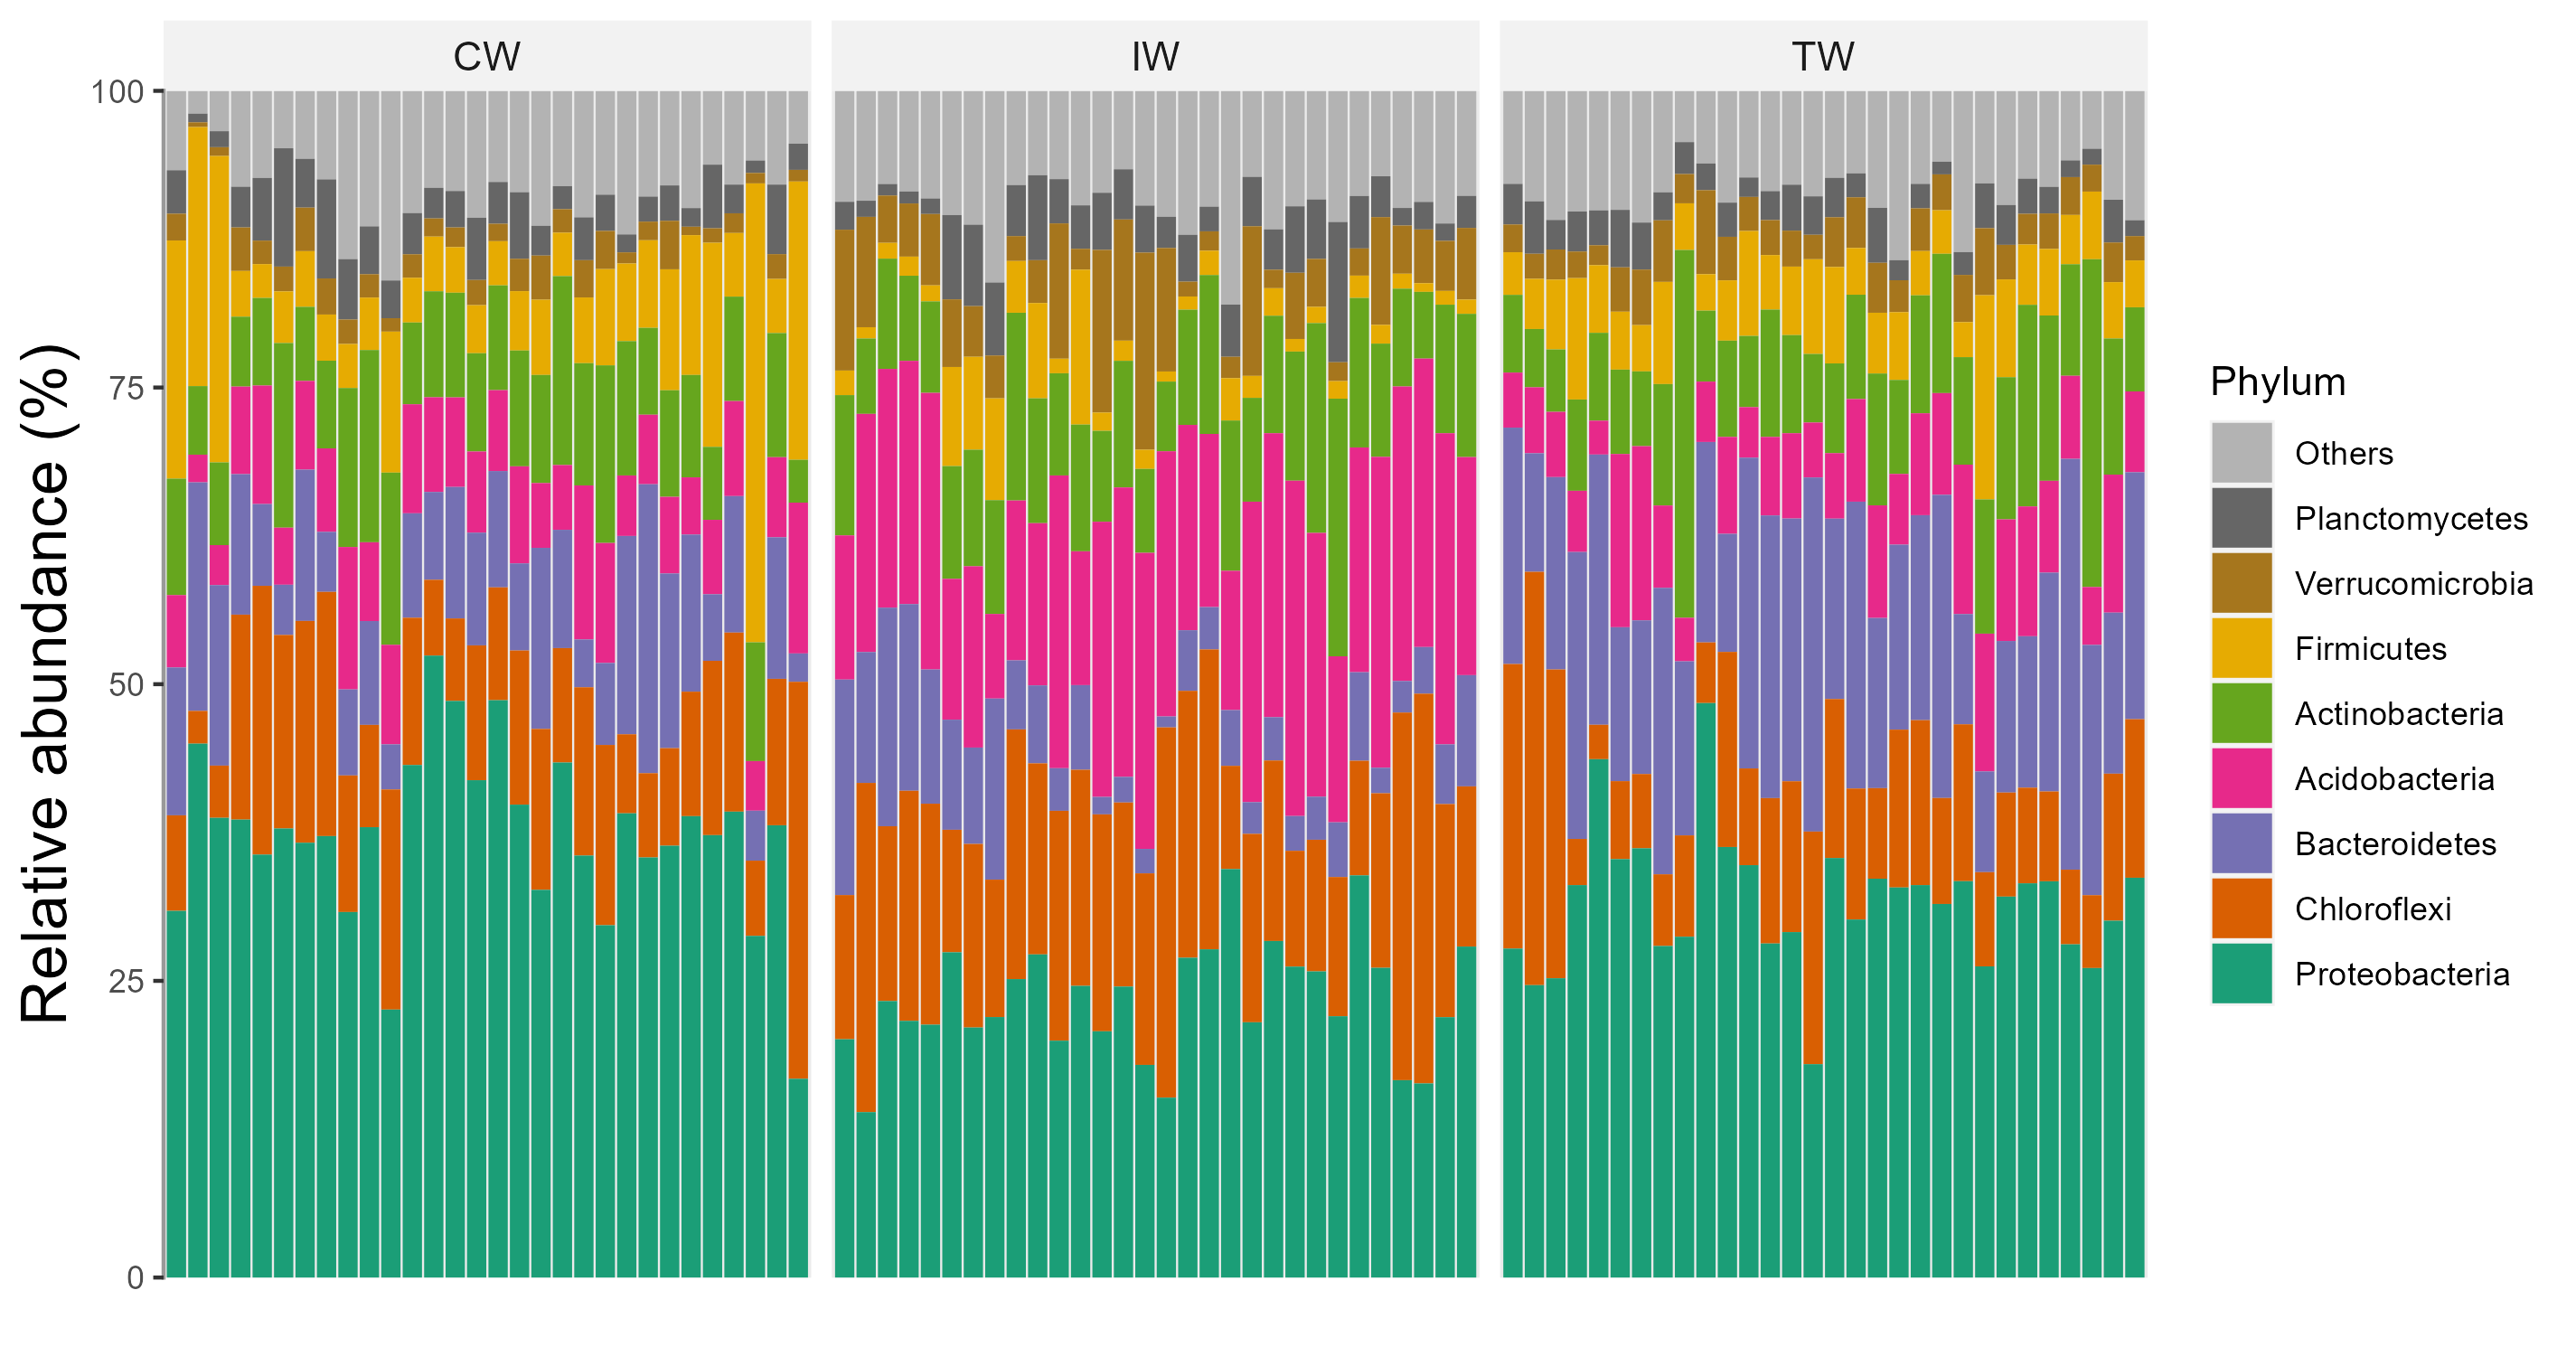
\includegraphics[width=750px]{Images/trans_abund_barplot1} \end{center}

Two or more facets are supported with the facet parameter from v0.14.0 by providing a vector with multiple elements.

\begin{Shaded}
\begin{Highlighting}[]
\CommentTok{\# require package ggh4x, first run install.packages("ggh4x") if not installed}
\NormalTok{t1}\SpecialCharTok{$}\FunctionTok{plot\_bar}\NormalTok{(}\AttributeTok{others\_color =} \StringTok{"grey70"}\NormalTok{, }\AttributeTok{facet =} \FunctionTok{c}\NormalTok{(}\StringTok{"Group"}\NormalTok{, }\StringTok{"Type"}\NormalTok{), }\AttributeTok{xtext\_keep =} \ConstantTok{FALSE}\NormalTok{, }\AttributeTok{legend\_text\_italic =} \ConstantTok{FALSE}\NormalTok{, }\AttributeTok{barwidth =} \DecValTok{1}\NormalTok{)}
\end{Highlighting}
\end{Shaded}

\begin{center}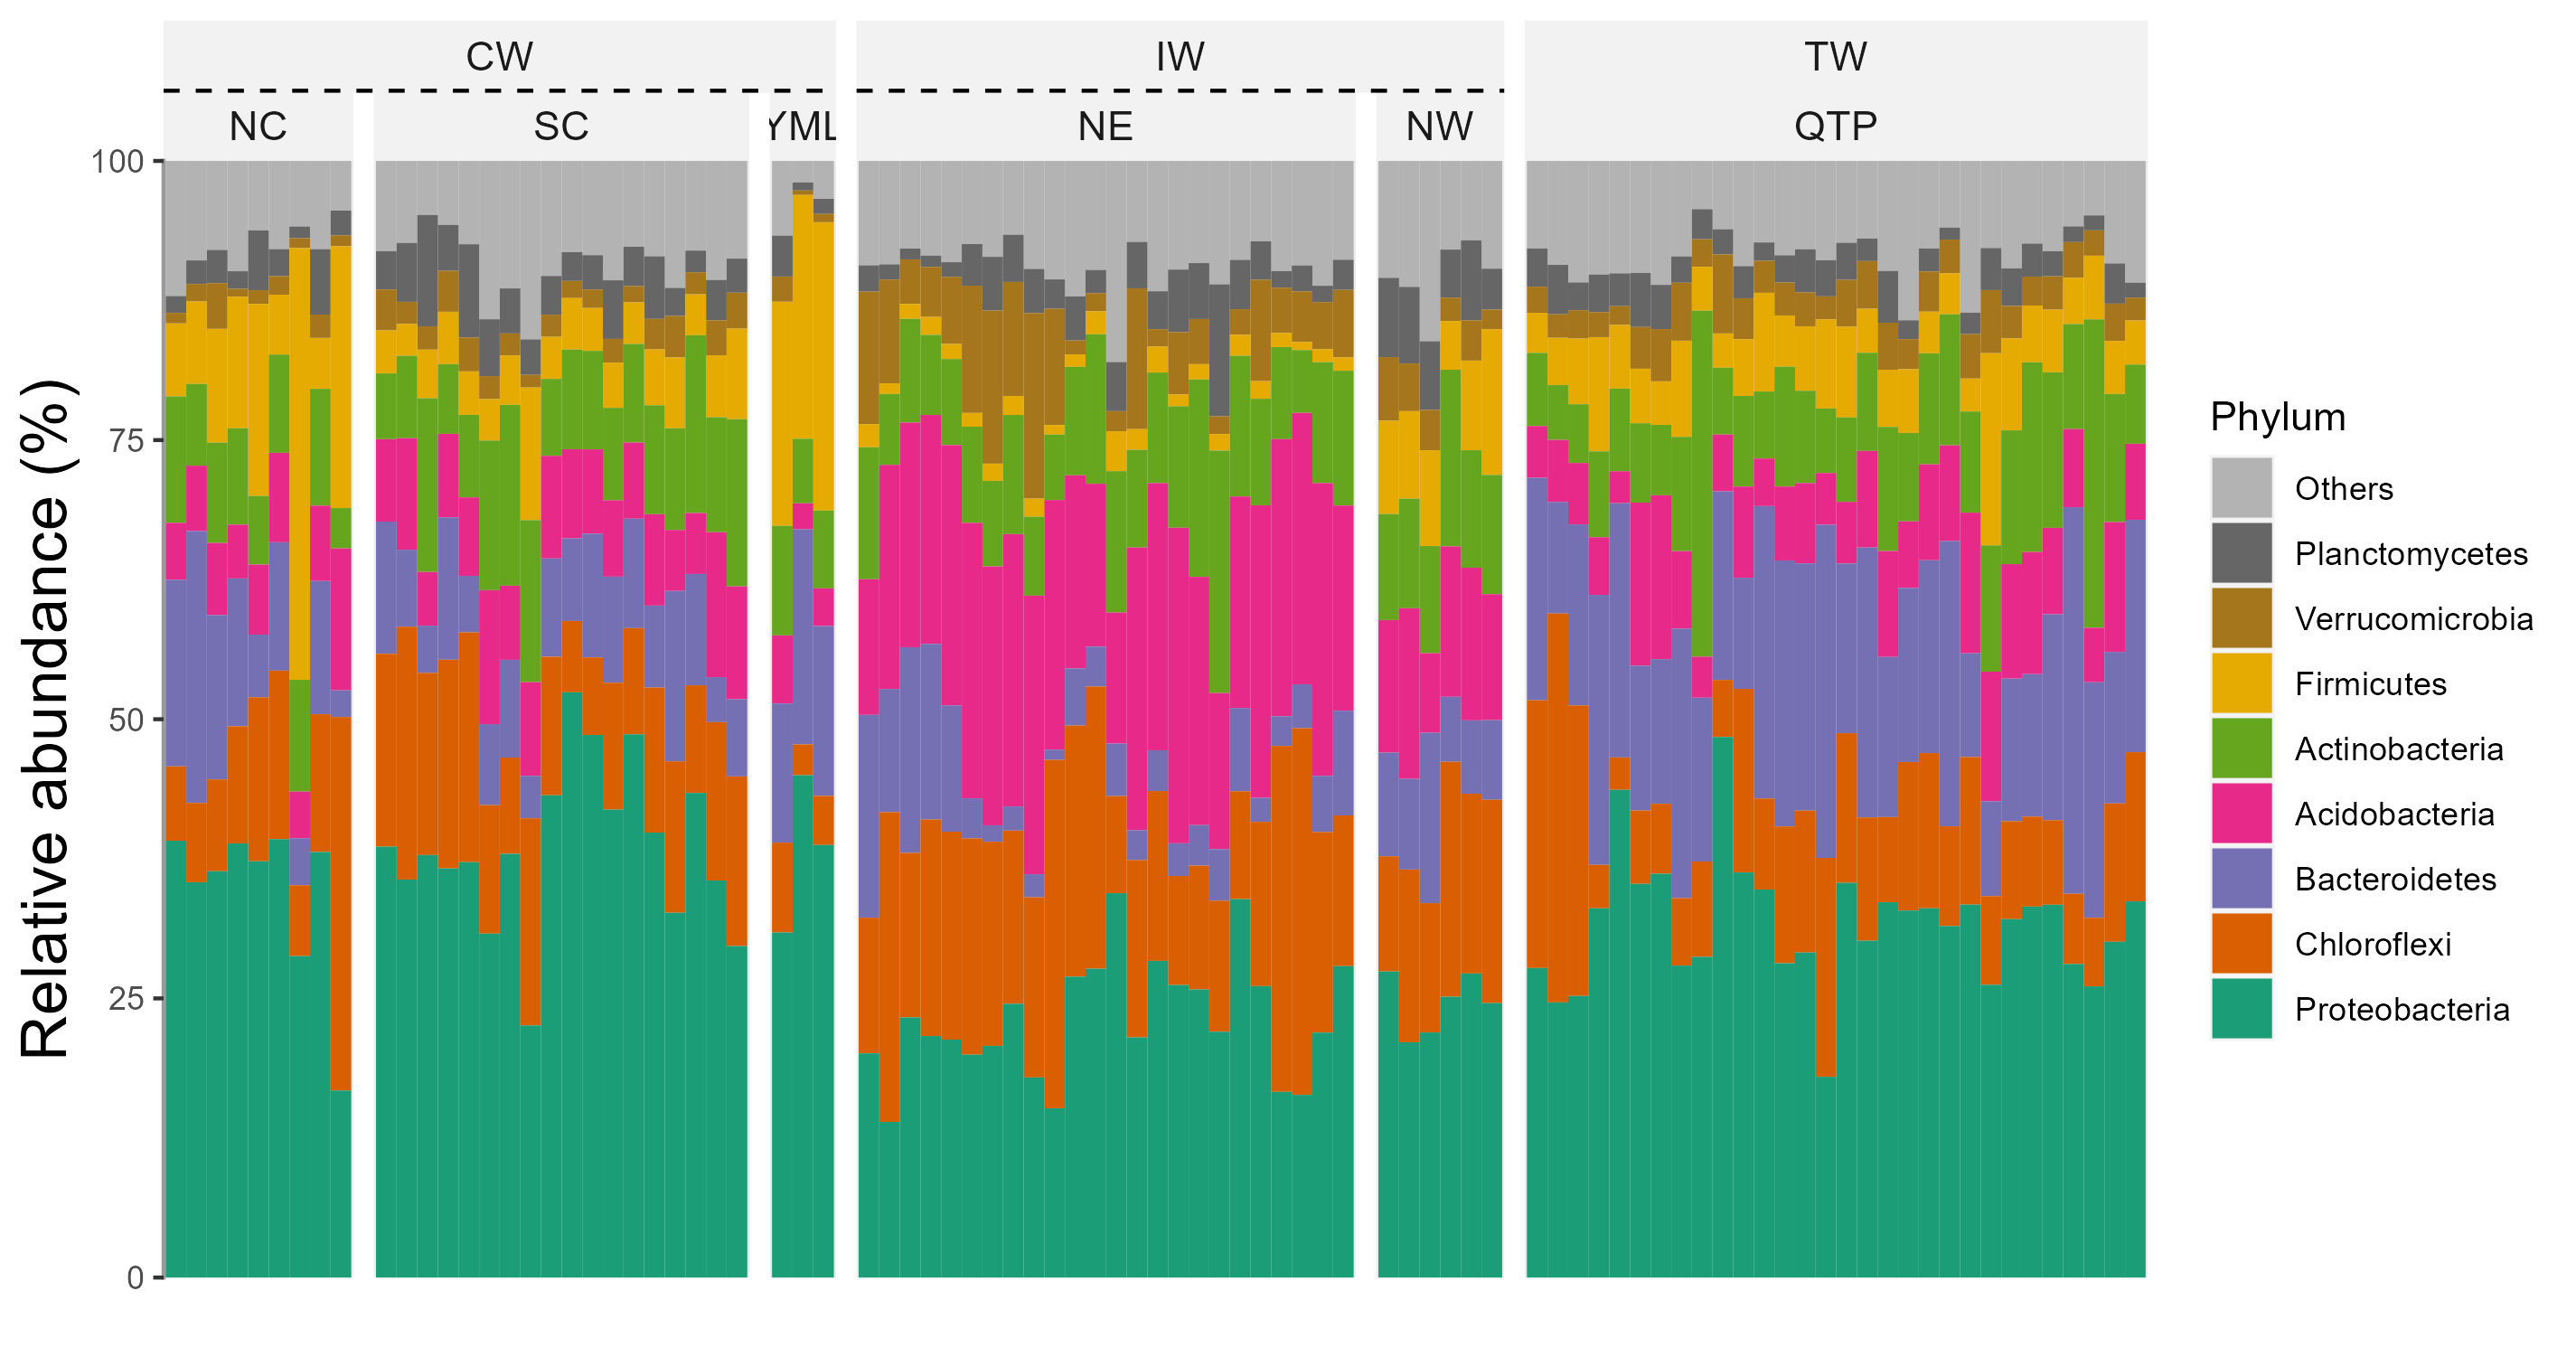
\includegraphics[width=750px]{Images/trans_abund_barplot_facet2} \end{center}

The default operation can filter all the unclassified taxa (i.e.~p\_\_ or g\_\_ in tax\_table that has been processed by \texttt{tidy\_taxonomy} function),
as those unknown taxa are generally meaningless.
However sometimes, these unknown taxa may be meaningful for users.
For example, if one want to isolate some unknown species, it is valuable to check the abundance of those unknown taxa.
At this time, please see this topic (\url{https://github.com/ChiLiubio/microeco/issues/165}) to resolve the issue that how to show unknown taxa with hierarchical taxonomy classification.
The alluvial plot is also implemented in the plot\_bar function with use\_alluvium parameter.

\begin{Shaded}
\begin{Highlighting}[]
\NormalTok{t1 }\OtherTok{\textless{}{-}}\NormalTok{ trans\_abund}\SpecialCharTok{$}\FunctionTok{new}\NormalTok{(}\AttributeTok{dataset =}\NormalTok{ dataset, }\AttributeTok{taxrank =} \StringTok{"Genus"}\NormalTok{, }\AttributeTok{ntaxa =} \DecValTok{8}\NormalTok{)}
\CommentTok{\# require ggalluvial package}
\CommentTok{\# use\_alluvium = TRUE make the alluvial plot, clustering =TRUE can be used to reorder the samples by clustering}
\CommentTok{\# bar\_type = "notfull" can discard \textquotesingle{}others\textquotesingle{}; select another color palette}
\NormalTok{p }\OtherTok{\textless{}{-}}\NormalTok{ t1}\SpecialCharTok{$}\FunctionTok{plot\_bar}\NormalTok{(}\AttributeTok{bar\_type =} \StringTok{"notfull"}\NormalTok{, }\AttributeTok{use\_alluvium =} \ConstantTok{TRUE}\NormalTok{, }\AttributeTok{clustering =} \ConstantTok{TRUE}\NormalTok{, }\AttributeTok{xtext\_angle =} \DecValTok{30}\NormalTok{, }\AttributeTok{xtext\_size =} \DecValTok{3}\NormalTok{, }\AttributeTok{color\_values =}\NormalTok{ RColorBrewer}\SpecialCharTok{::}\FunctionTok{brewer.pal}\NormalTok{(}\DecValTok{8}\NormalTok{, }\StringTok{"Set2"}\NormalTok{))}
\end{Highlighting}
\end{Shaded}

\begin{center}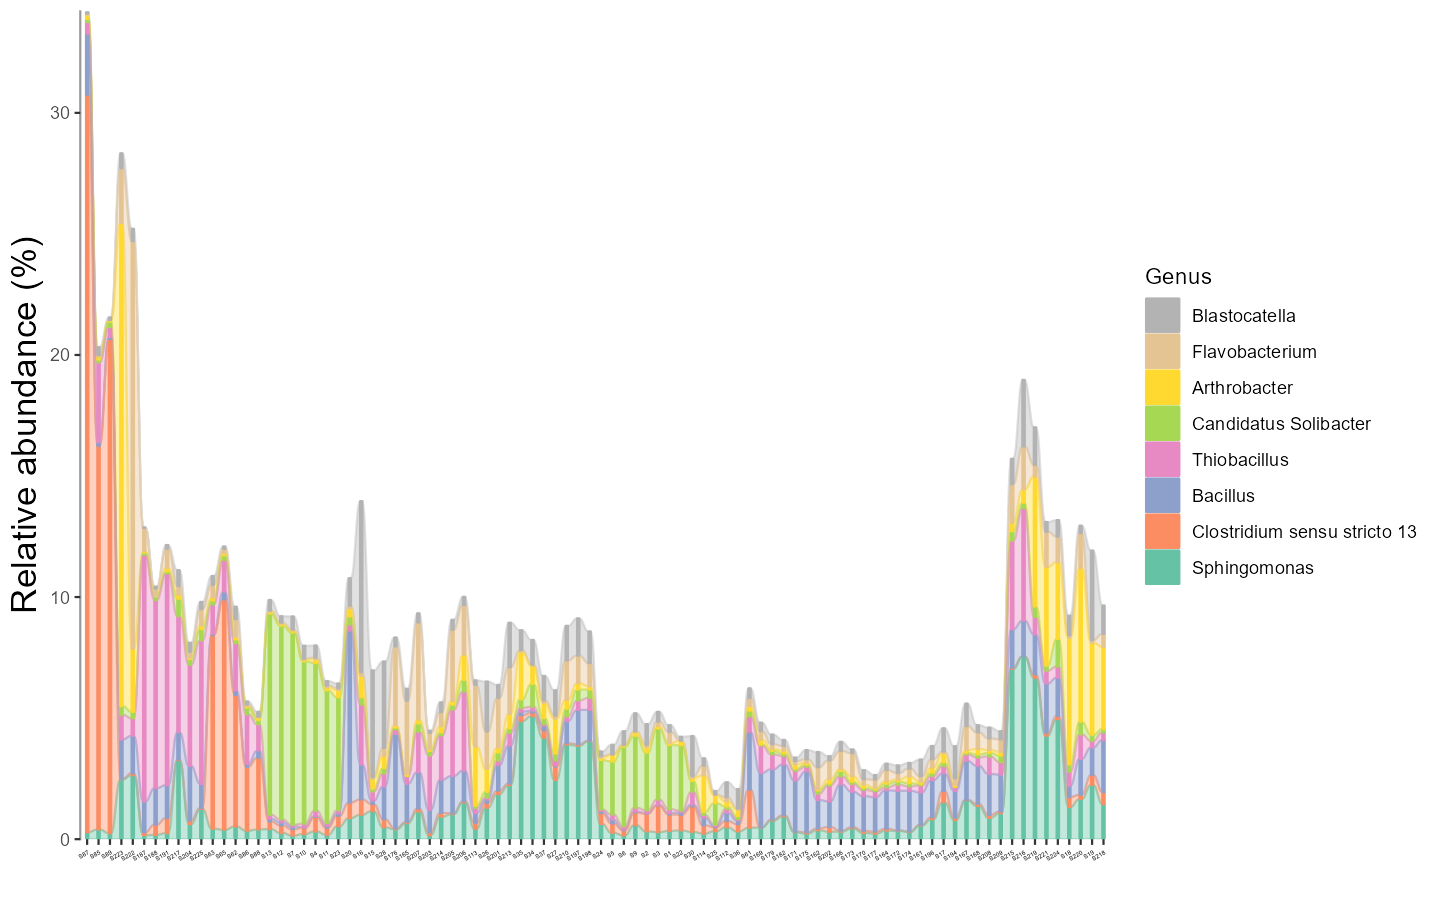
\includegraphics[width=20in]{Images/trans_abund_bar_allu} \end{center}

The bar plot can also be performed with group mean values.
Note that, from v0.16.0, the parameter \texttt{group\_morestats\ =\ TRUE} can be used to add more summary statistics in the return \texttt{data\_abund} when \texttt{groupmean} parameter is provided.

\begin{Shaded}
\begin{Highlighting}[]
\CommentTok{\# The groupmean parameter can be used to obtain the group{-}mean barplot.}
\NormalTok{t1 }\OtherTok{\textless{}{-}}\NormalTok{ trans\_abund}\SpecialCharTok{$}\FunctionTok{new}\NormalTok{(}\AttributeTok{dataset =}\NormalTok{ dataset, }\AttributeTok{taxrank =} \StringTok{"Phylum"}\NormalTok{, }\AttributeTok{ntaxa =} \DecValTok{10}\NormalTok{, }\AttributeTok{groupmean =} \StringTok{"Group"}\NormalTok{)}
\NormalTok{g1 }\OtherTok{\textless{}{-}}\NormalTok{ t1}\SpecialCharTok{$}\FunctionTok{plot\_bar}\NormalTok{(}\AttributeTok{others\_color =} \StringTok{"grey70"}\NormalTok{, }\AttributeTok{legend\_text\_italic =} \ConstantTok{FALSE}\NormalTok{)}
\NormalTok{g1 }\SpecialCharTok{+} \FunctionTok{theme\_classic}\NormalTok{() }\SpecialCharTok{+} \FunctionTok{theme}\NormalTok{(}\AttributeTok{axis.title.y =} \FunctionTok{element\_text}\NormalTok{(}\AttributeTok{size =} \DecValTok{18}\NormalTok{))}
\end{Highlighting}
\end{Shaded}

\begin{center}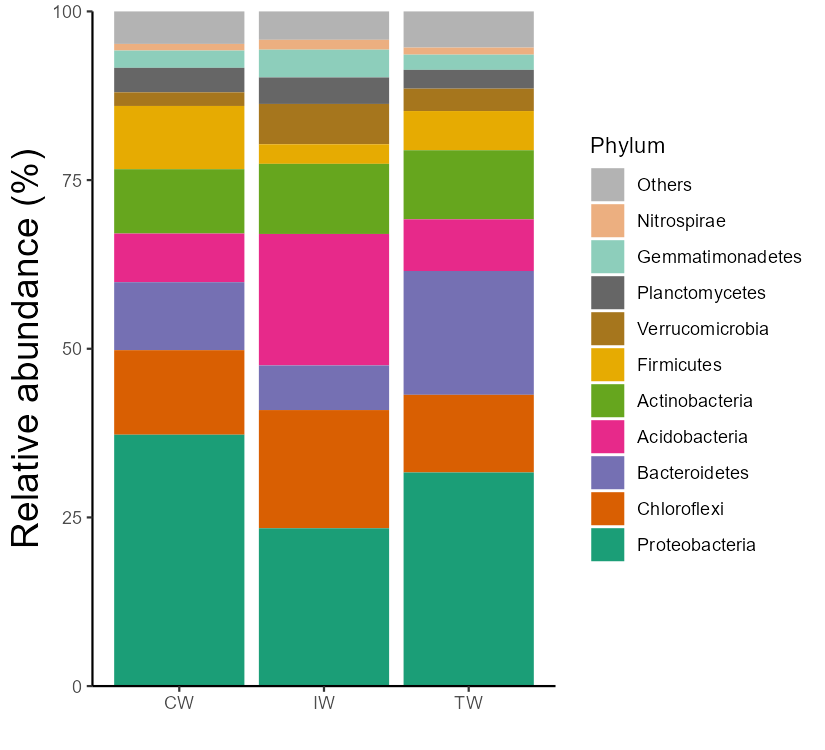
\includegraphics[width=400px]{Images/trans_abund_barplot_groupmean} \end{center}

The box plot is an excellent way to intuitionally show abundance distribution across groups.

\begin{Shaded}
\begin{Highlighting}[]
\CommentTok{\# show 15 taxa at Class level}
\NormalTok{t1 }\OtherTok{\textless{}{-}}\NormalTok{ trans\_abund}\SpecialCharTok{$}\FunctionTok{new}\NormalTok{(}\AttributeTok{dataset =}\NormalTok{ dataset, }\AttributeTok{taxrank =} \StringTok{"Class"}\NormalTok{, }\AttributeTok{ntaxa =} \DecValTok{15}\NormalTok{)}
\NormalTok{t1}\SpecialCharTok{$}\FunctionTok{plot\_box}\NormalTok{(}\AttributeTok{group =} \StringTok{"Group"}\NormalTok{, }\AttributeTok{xtext\_angle =} \DecValTok{30}\NormalTok{)}
\end{Highlighting}
\end{Shaded}

\begin{center}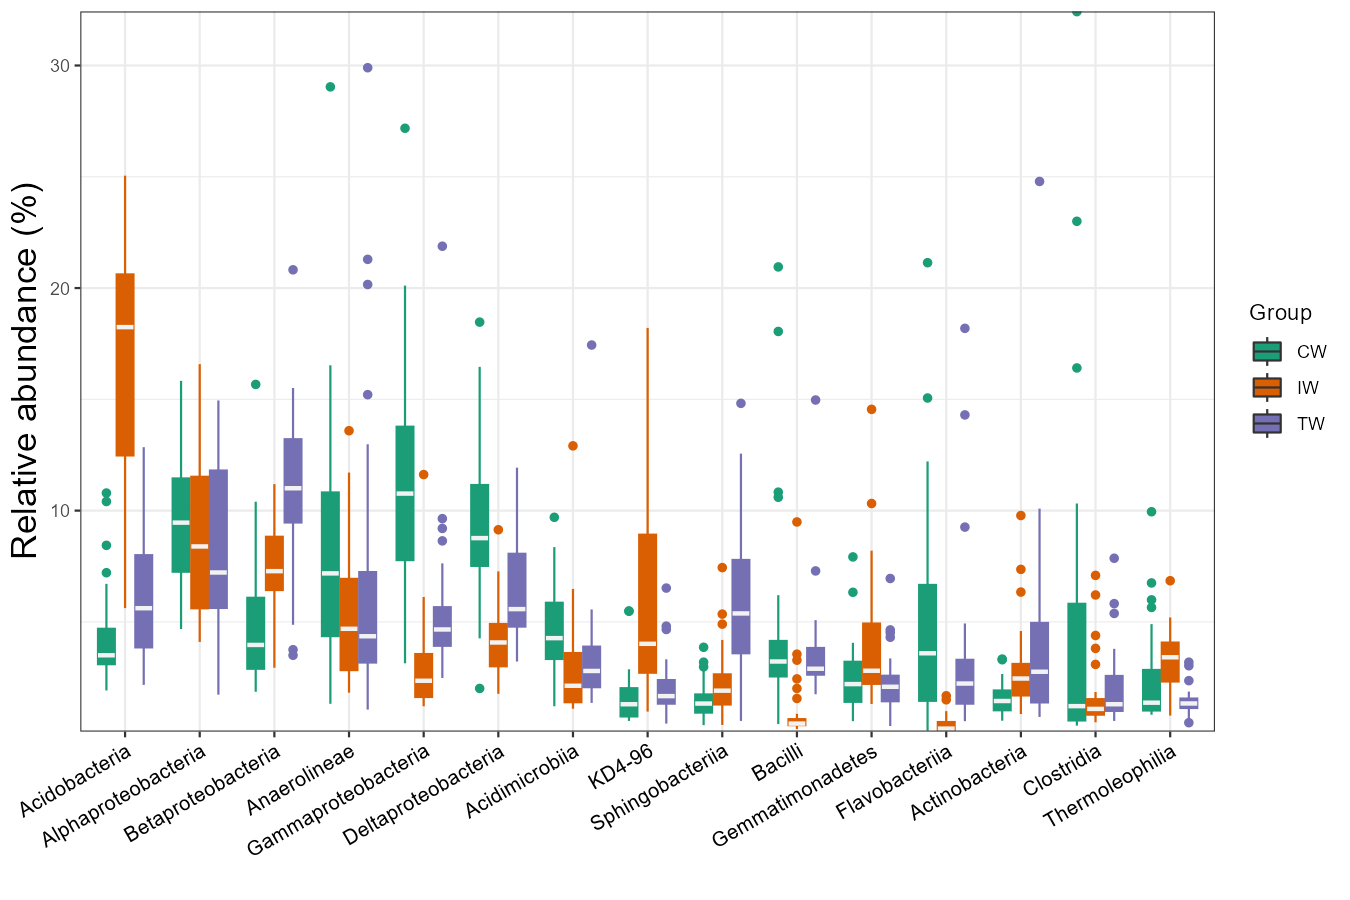
\includegraphics[width=700px]{Images/trans_abund_boxplot} \end{center}

Then we show the heatmap with the high abundant genera.

\begin{Shaded}
\begin{Highlighting}[]
\CommentTok{\# show 40 taxa at Genus level}
\NormalTok{t1 }\OtherTok{\textless{}{-}}\NormalTok{ trans\_abund}\SpecialCharTok{$}\FunctionTok{new}\NormalTok{(}\AttributeTok{dataset =}\NormalTok{ dataset, }\AttributeTok{taxrank =} \StringTok{"Genus"}\NormalTok{, }\AttributeTok{ntaxa =} \DecValTok{40}\NormalTok{)}
\NormalTok{t1}\SpecialCharTok{$}\FunctionTok{plot\_heatmap}\NormalTok{(}\AttributeTok{facet =} \StringTok{"Group"}\NormalTok{, }\AttributeTok{xtext\_keep =} \ConstantTok{FALSE}\NormalTok{, }\AttributeTok{withmargin =} \ConstantTok{FALSE}\NormalTok{)}
\end{Highlighting}
\end{Shaded}

\begin{center}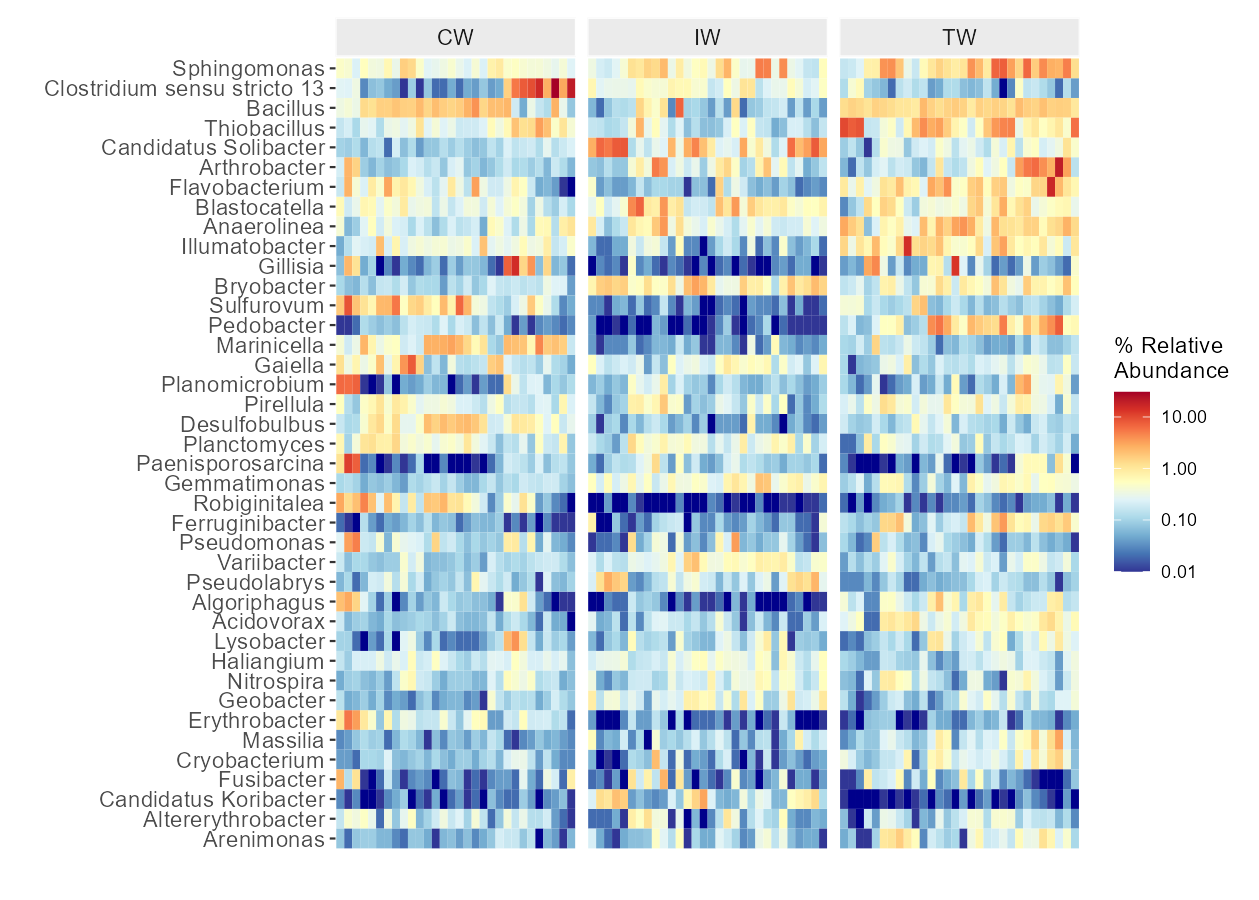
\includegraphics[width=750px]{Images/trans_abund_heatmap} \end{center}

Line chart is very useful to show the abundance change of taxa along time, space or other gradients.

\begin{Shaded}
\begin{Highlighting}[]
\NormalTok{t1 }\OtherTok{\textless{}{-}}\NormalTok{ trans\_abund}\SpecialCharTok{$}\FunctionTok{new}\NormalTok{(}\AttributeTok{dataset =}\NormalTok{ dataset, }\AttributeTok{taxrank =} \StringTok{"Phylum"}\NormalTok{, }\AttributeTok{ntaxa =} \DecValTok{5}\NormalTok{)}
\NormalTok{t1}\SpecialCharTok{$}\FunctionTok{plot\_line}\NormalTok{()}
\NormalTok{t1 }\OtherTok{\textless{}{-}}\NormalTok{ trans\_abund}\SpecialCharTok{$}\FunctionTok{new}\NormalTok{(}\AttributeTok{dataset =}\NormalTok{ dataset, }\AttributeTok{taxrank =} \StringTok{"Genus"}\NormalTok{, }\AttributeTok{ntaxa =} \DecValTok{5}\NormalTok{, }\AttributeTok{groupmean =} \StringTok{"Type"}\NormalTok{)}
\NormalTok{t1}\SpecialCharTok{$}\FunctionTok{plot\_line}\NormalTok{(}\AttributeTok{position =} \FunctionTok{position\_dodge}\NormalTok{(}\FloatTok{0.3}\NormalTok{), }\AttributeTok{xtext\_angle =} \DecValTok{0}\NormalTok{)}
\end{Highlighting}
\end{Shaded}

\begin{center}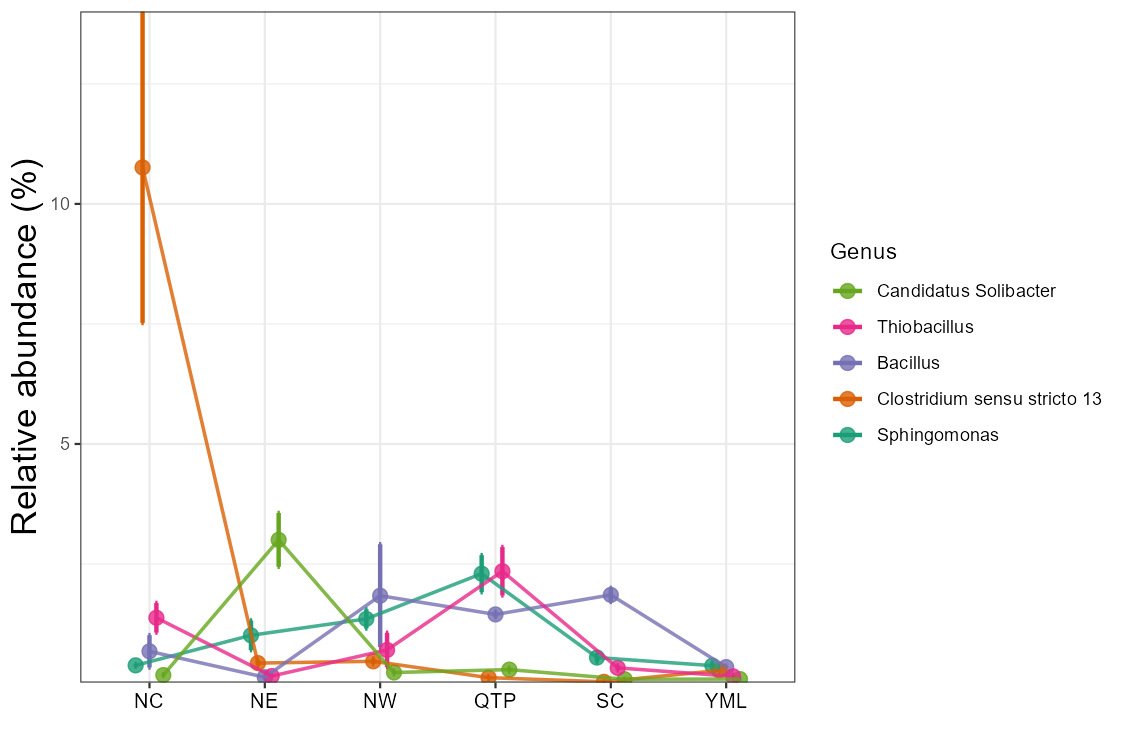
\includegraphics[width=750px]{Images/trans_abund_line} \end{center}

Then, we show the pie chart with the group mean values.

\begin{Shaded}
\begin{Highlighting}[]
\NormalTok{t1 }\OtherTok{\textless{}{-}}\NormalTok{ trans\_abund}\SpecialCharTok{$}\FunctionTok{new}\NormalTok{(}\AttributeTok{dataset =}\NormalTok{ dataset, }\AttributeTok{taxrank =} \StringTok{"Phylum"}\NormalTok{, }\AttributeTok{ntaxa =} \DecValTok{6}\NormalTok{, }\AttributeTok{groupmean =} \StringTok{"Group"}\NormalTok{)}
\CommentTok{\# all pie chart in one row}
\NormalTok{t1}\SpecialCharTok{$}\FunctionTok{plot\_pie}\NormalTok{(}\AttributeTok{facet\_nrow =} \DecValTok{1}\NormalTok{)}
\NormalTok{t1}\SpecialCharTok{$}\FunctionTok{plot\_pie}\NormalTok{(}\AttributeTok{facet\_nrow =} \DecValTok{1}\NormalTok{, }\AttributeTok{add\_label =} \ConstantTok{TRUE}\NormalTok{)}
\end{Highlighting}
\end{Shaded}

\begin{center}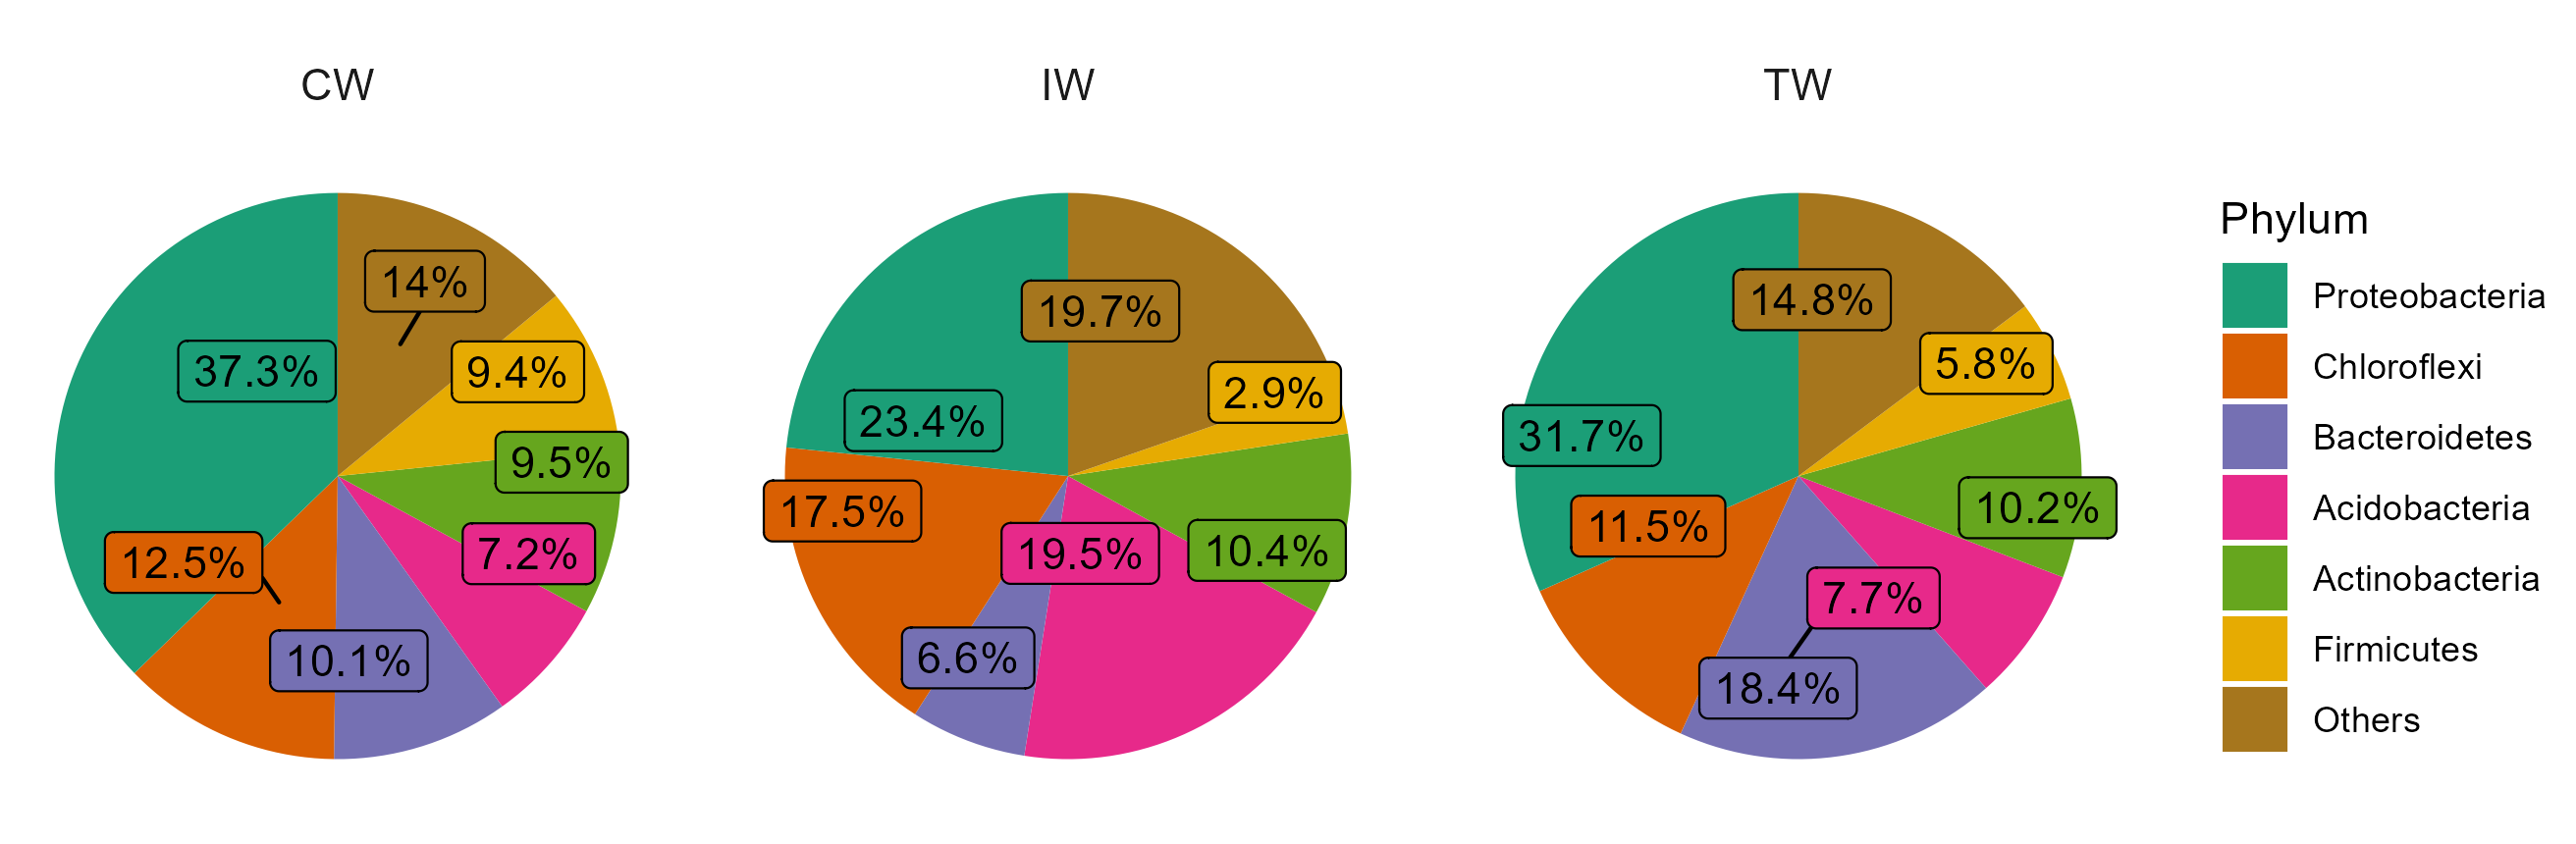
\includegraphics[width=600px]{Images/trans_abund_pie} \end{center}

The donut and radar charts are implemented from v0.17.0.
Please install the dependent packages according to the steps (\url{https://chiliubio.github.io/microeco_tutorial/intro.html\#dependence}).

\begin{Shaded}
\begin{Highlighting}[]
\NormalTok{t1 }\OtherTok{\textless{}{-}}\NormalTok{ trans\_abund}\SpecialCharTok{$}\FunctionTok{new}\NormalTok{(}\AttributeTok{dataset =}\NormalTok{ dataset, }\AttributeTok{taxrank =} \StringTok{"Phylum"}\NormalTok{, }\AttributeTok{ntaxa =} \DecValTok{8}\NormalTok{, }\AttributeTok{groupmean =} \StringTok{"Group"}\NormalTok{)}
\NormalTok{t1}\SpecialCharTok{$}\FunctionTok{plot\_donut}\NormalTok{(}\AttributeTok{label =} \ConstantTok{FALSE}\NormalTok{)}
\NormalTok{t1}\SpecialCharTok{$}\FunctionTok{plot\_donut}\NormalTok{(}\AttributeTok{label =} \ConstantTok{TRUE}\NormalTok{)}
\end{Highlighting}
\end{Shaded}

\begin{center}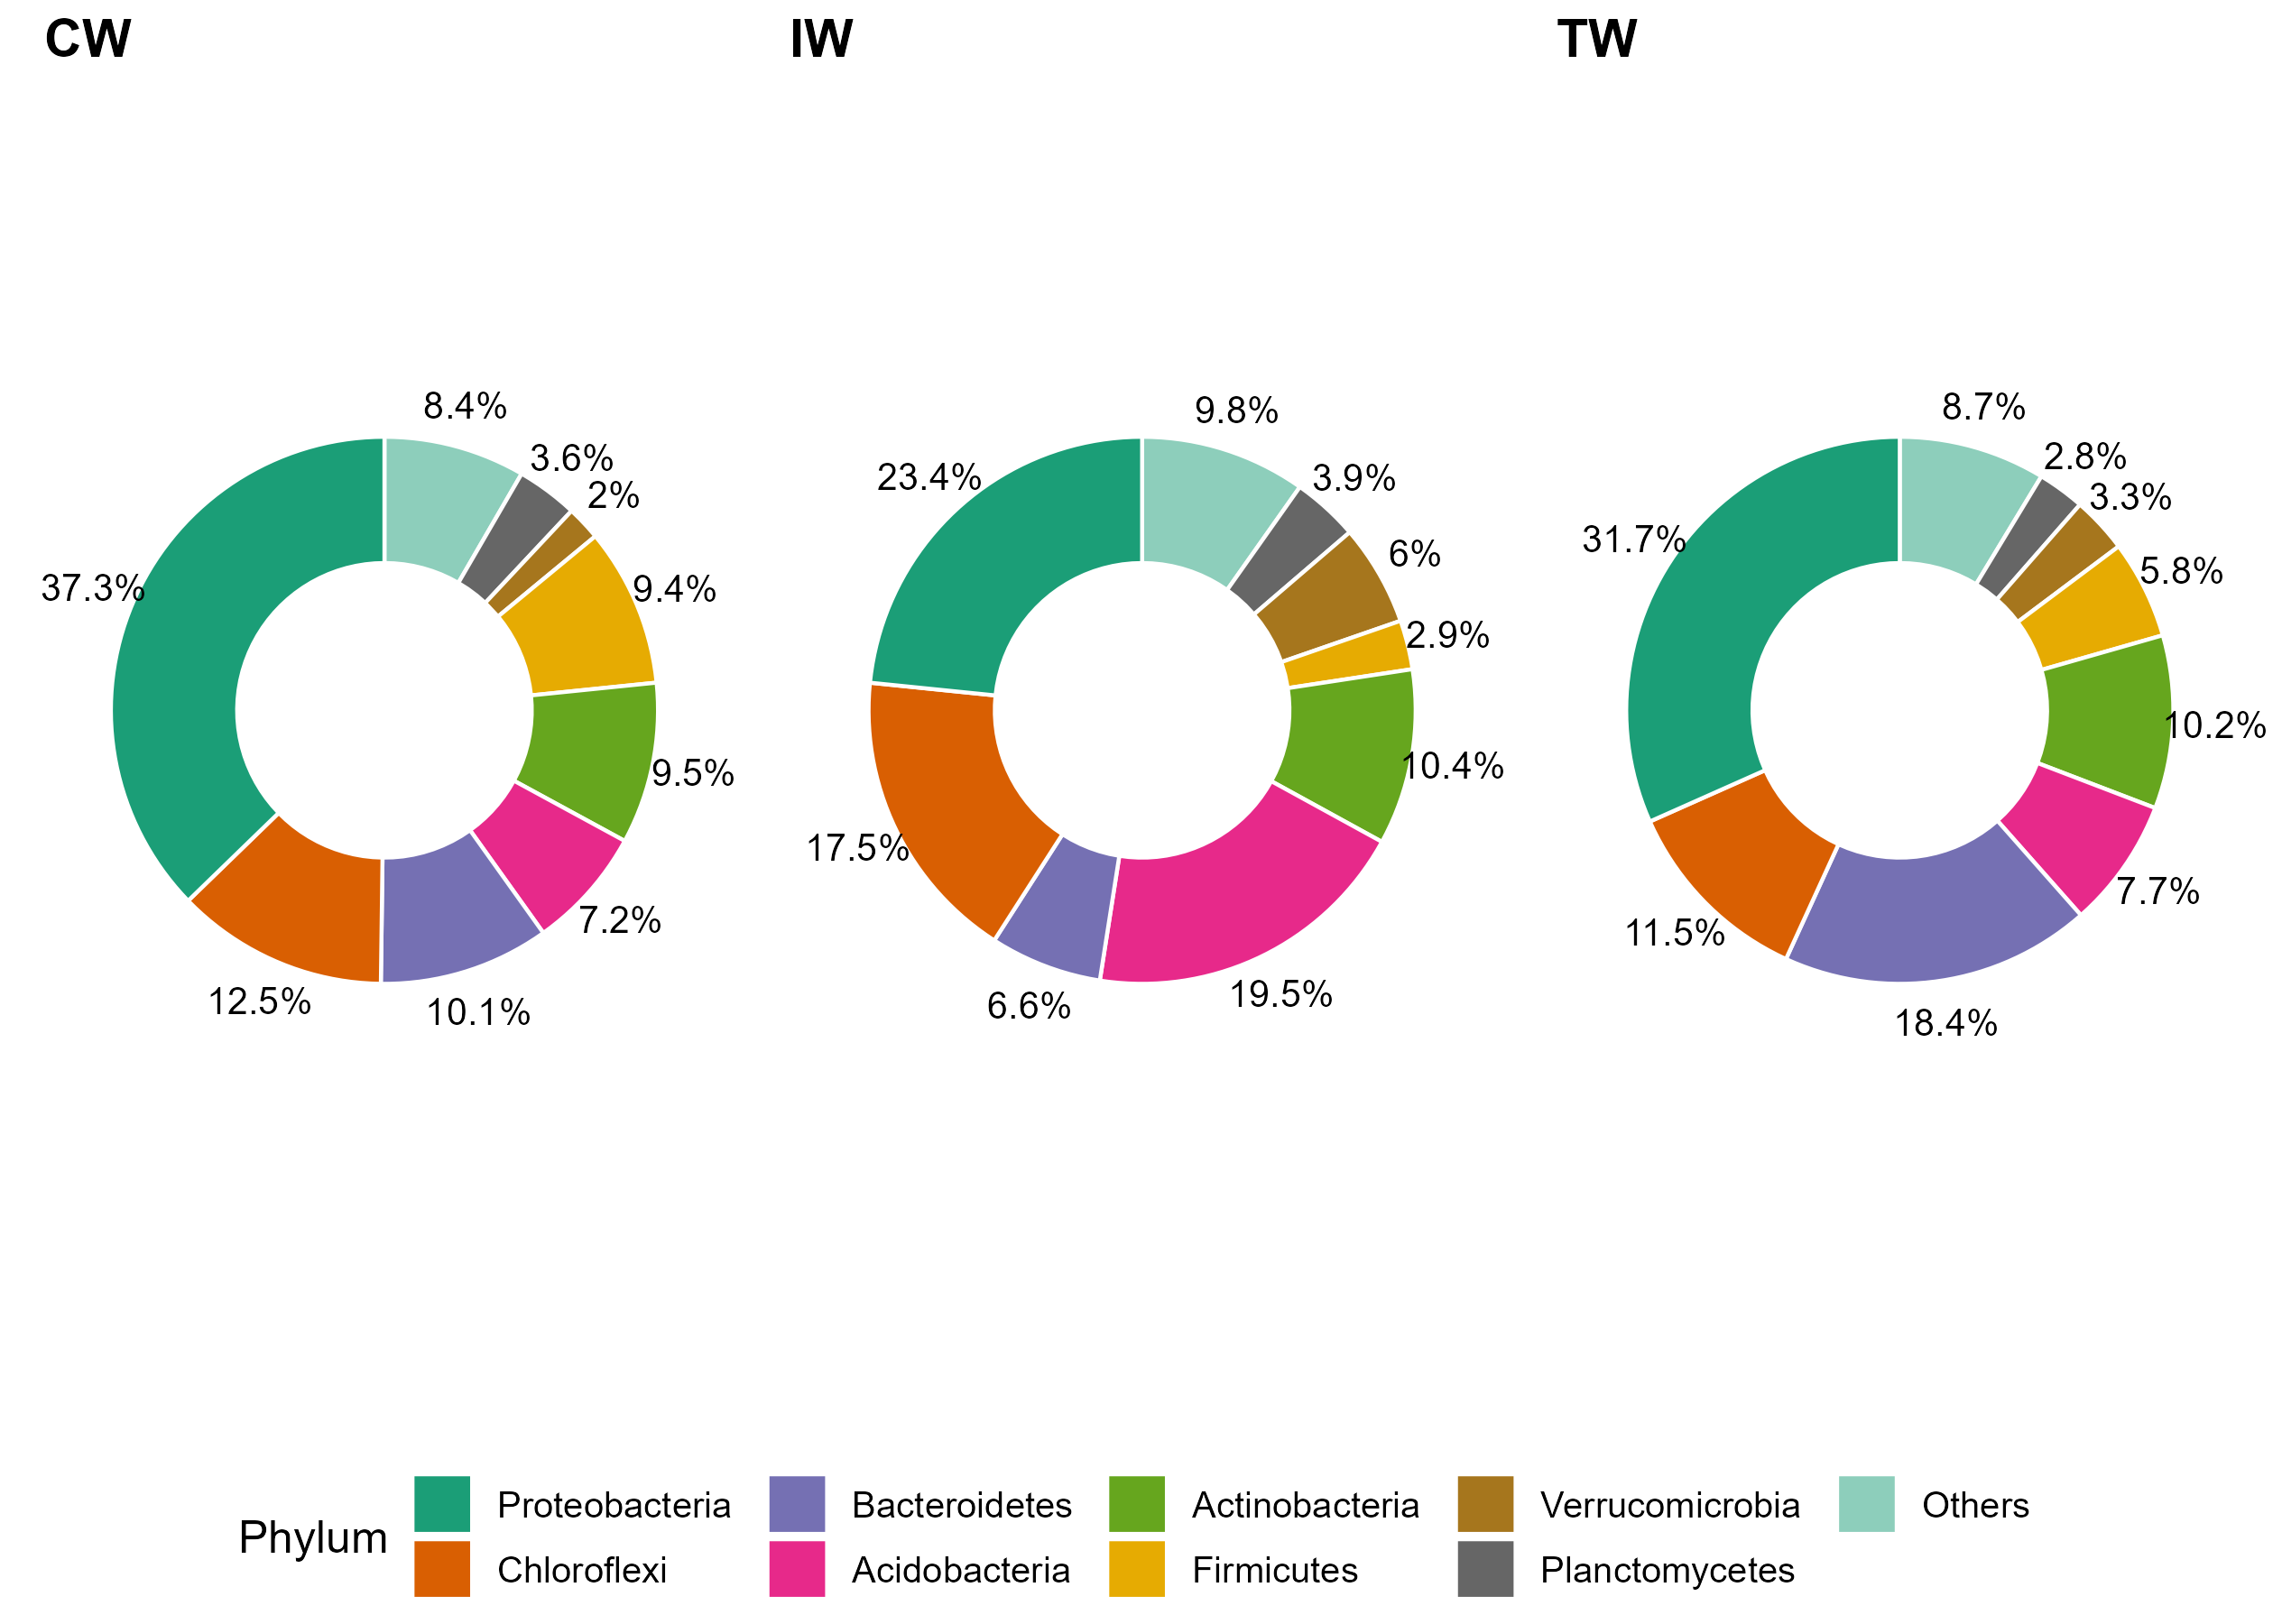
\includegraphics[width=650px]{Images/trans_abund_donut} \end{center}

\begin{Shaded}
\begin{Highlighting}[]
\NormalTok{t1 }\OtherTok{\textless{}{-}}\NormalTok{ trans\_abund}\SpecialCharTok{$}\FunctionTok{new}\NormalTok{(}\AttributeTok{dataset =}\NormalTok{ dataset, }\AttributeTok{taxrank =} \StringTok{"Phylum"}\NormalTok{, }\AttributeTok{ntaxa =} \DecValTok{8}\NormalTok{, }\AttributeTok{groupmean =} \StringTok{"Group"}\NormalTok{)}
\NormalTok{t1}\SpecialCharTok{$}\FunctionTok{plot\_radar}\NormalTok{(}\AttributeTok{values.radar =} \FunctionTok{c}\NormalTok{(}\StringTok{"0\%"}\NormalTok{, }\StringTok{"25\%"}\NormalTok{, }\StringTok{"50\%"}\NormalTok{), }\AttributeTok{grid.min =} \DecValTok{0}\NormalTok{, }\AttributeTok{grid.mid =} \FloatTok{0.25}\NormalTok{, }\AttributeTok{grid.max =} \FloatTok{0.5}\NormalTok{)}
\NormalTok{t1 }\OtherTok{\textless{}{-}}\NormalTok{ trans\_abund}\SpecialCharTok{$}\FunctionTok{new}\NormalTok{(}\AttributeTok{dataset =}\NormalTok{ dataset, }\AttributeTok{taxrank =} \StringTok{"Phylum"}\NormalTok{, }\AttributeTok{ntaxa =} \DecValTok{8}\NormalTok{, }\AttributeTok{groupmean =} \StringTok{"Type"}\NormalTok{)}
\NormalTok{t1}\SpecialCharTok{$}\FunctionTok{plot\_radar}\NormalTok{(}\AttributeTok{values.radar =} \FunctionTok{c}\NormalTok{(}\StringTok{"0\%"}\NormalTok{, }\StringTok{"25\%"}\NormalTok{, }\StringTok{"50\%"}\NormalTok{), }\AttributeTok{grid.min =} \DecValTok{0}\NormalTok{, }\AttributeTok{grid.mid =} \FloatTok{0.25}\NormalTok{, }\AttributeTok{grid.max =} \FloatTok{0.5}\NormalTok{)}
\end{Highlighting}
\end{Shaded}

\begin{center}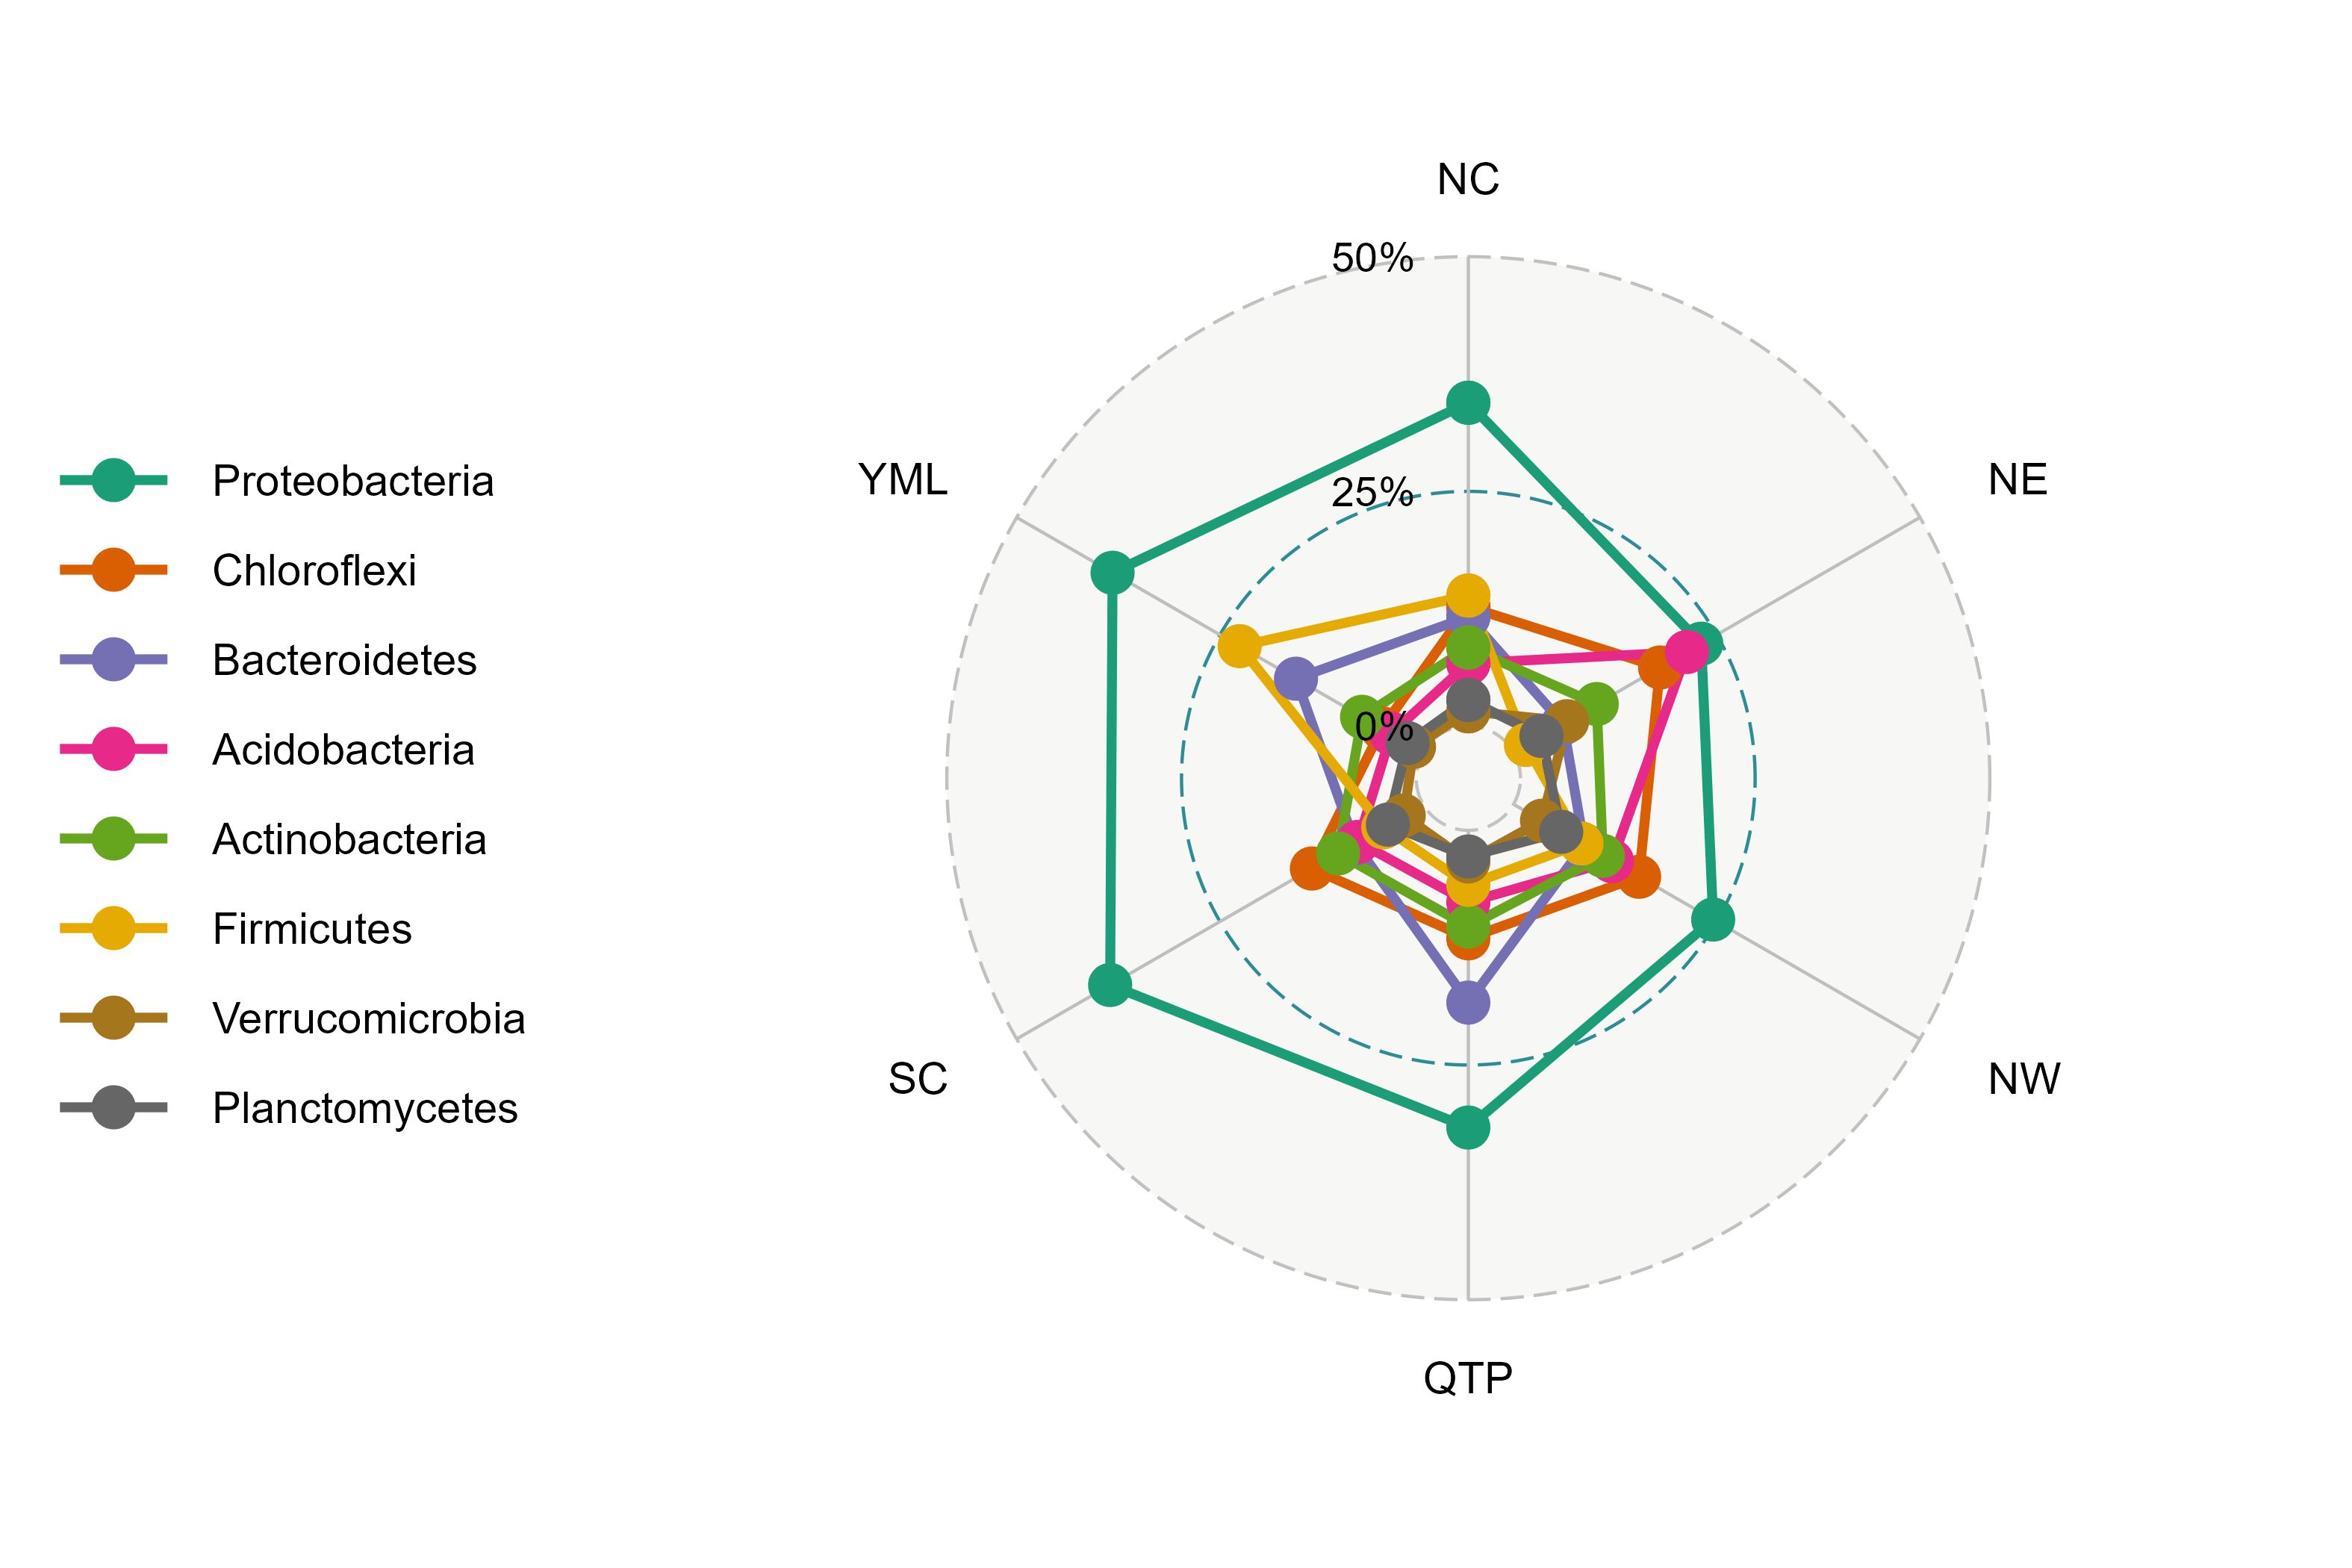
\includegraphics[width=700px]{Images/trans_abund_radar} \end{center}

The ternary plot can be used for the case with three samples/groups.

\begin{Shaded}
\begin{Highlighting}[]
\NormalTok{t1 }\OtherTok{\textless{}{-}}\NormalTok{ trans\_abund}\SpecialCharTok{$}\FunctionTok{new}\NormalTok{(}\AttributeTok{dataset =}\NormalTok{ dataset, }\AttributeTok{taxrank =} \StringTok{"Phylum"}\NormalTok{, }\AttributeTok{ntaxa =} \DecValTok{8}\NormalTok{, }\AttributeTok{groupmean =} \StringTok{"Group"}\NormalTok{)}
\NormalTok{t1}\SpecialCharTok{$}\FunctionTok{plot\_tern}\NormalTok{()}
\end{Highlighting}
\end{Shaded}

\begin{center}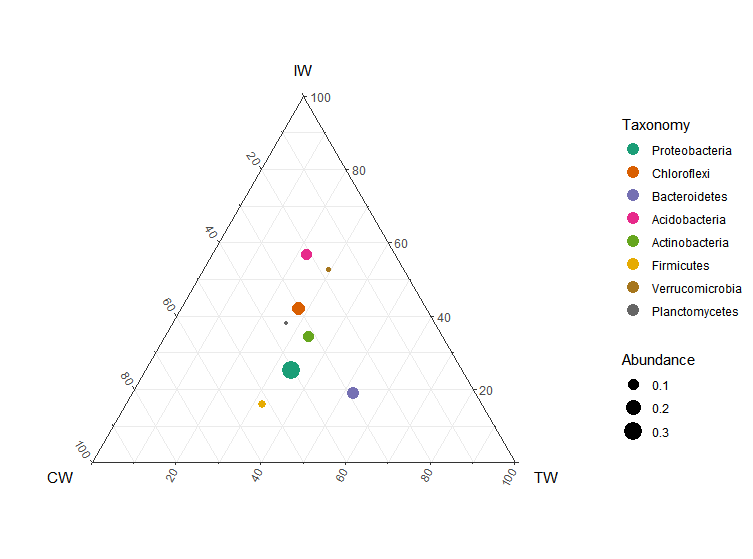
\includegraphics[width=600px]{Images/trans_abund_ternary} \end{center}

When the hierarchical abundance data of two levels is needed to be shown in bar plot, the nested legend can be used.

\begin{Shaded}
\begin{Highlighting}[]
\CommentTok{\# require ggnested package; see https://chiliubio.github.io/microeco\_tutorial/intro.html\#dependence}
\NormalTok{test1 }\OtherTok{\textless{}{-}}\NormalTok{ trans\_abund}\SpecialCharTok{$}\FunctionTok{new}\NormalTok{(}\AttributeTok{dataset =}\NormalTok{ dataset, }\AttributeTok{taxrank =} \StringTok{"Class"}\NormalTok{, }\AttributeTok{ntaxa =} \DecValTok{10}\NormalTok{, }\AttributeTok{high\_level =} \StringTok{"Phylum"}\NormalTok{, }\AttributeTok{prefix =} \StringTok{"}\SpecialCharTok{\textbackslash{}\textbackslash{}}\StringTok{|"}\NormalTok{)}
\NormalTok{test1}\SpecialCharTok{$}\FunctionTok{plot\_bar}\NormalTok{(}\AttributeTok{ggnested =} \ConstantTok{TRUE}\NormalTok{, }\AttributeTok{facet =} \FunctionTok{c}\NormalTok{(}\StringTok{"Group"}\NormalTok{, }\StringTok{"Type"}\NormalTok{), }\AttributeTok{xtext\_angle =} \DecValTok{30}\NormalTok{)}
\CommentTok{\# fixed number in each phylum}
\NormalTok{test1 }\OtherTok{\textless{}{-}}\NormalTok{ trans\_abund}\SpecialCharTok{$}\FunctionTok{new}\NormalTok{(}\AttributeTok{dataset =}\NormalTok{ dataset, }\AttributeTok{taxrank =} \StringTok{"Class"}\NormalTok{, }\AttributeTok{ntaxa =} \DecValTok{30}\NormalTok{, }\AttributeTok{show =} \DecValTok{0}\NormalTok{, }\AttributeTok{high\_level =} \StringTok{"Phylum"}\NormalTok{, }\AttributeTok{high\_level\_fix\_nsub =} \DecValTok{4}\NormalTok{)}
\NormalTok{test1}\SpecialCharTok{$}\FunctionTok{plot\_bar}\NormalTok{(}\AttributeTok{ggnested =} \ConstantTok{TRUE}\NormalTok{, }\AttributeTok{xtext\_angle =} \DecValTok{30}\NormalTok{, }\AttributeTok{facet =} \FunctionTok{c}\NormalTok{(}\StringTok{"Group"}\NormalTok{, }\StringTok{"Type"}\NormalTok{))}
\CommentTok{\# sum others in each phylum}
\NormalTok{test1 }\OtherTok{\textless{}{-}}\NormalTok{ trans\_abund}\SpecialCharTok{$}\FunctionTok{new}\NormalTok{(}\AttributeTok{dataset =}\NormalTok{ dataset, }\AttributeTok{taxrank =} \StringTok{"Class"}\NormalTok{, }\AttributeTok{ntaxa =} \DecValTok{20}\NormalTok{, }\AttributeTok{show =} \DecValTok{0}\NormalTok{, }\AttributeTok{high\_level =} \StringTok{"Phylum"}\NormalTok{, }\AttributeTok{high\_level\_fix\_nsub =} \DecValTok{3}\NormalTok{, }\AttributeTok{prefix =} \StringTok{"}\SpecialCharTok{\textbackslash{}\textbackslash{}}\StringTok{|"}\NormalTok{)}
\NormalTok{test1}\SpecialCharTok{$}\FunctionTok{plot\_bar}\NormalTok{(}\AttributeTok{ggnested =} \ConstantTok{TRUE}\NormalTok{, }\AttributeTok{high\_level\_add\_other =} \ConstantTok{TRUE}\NormalTok{, }\AttributeTok{xtext\_angle =} \DecValTok{30}\NormalTok{, }\AttributeTok{facet =} \FunctionTok{c}\NormalTok{(}\StringTok{"Group"}\NormalTok{, }\StringTok{"Type"}\NormalTok{))}
\end{Highlighting}
\end{Shaded}

\begin{center}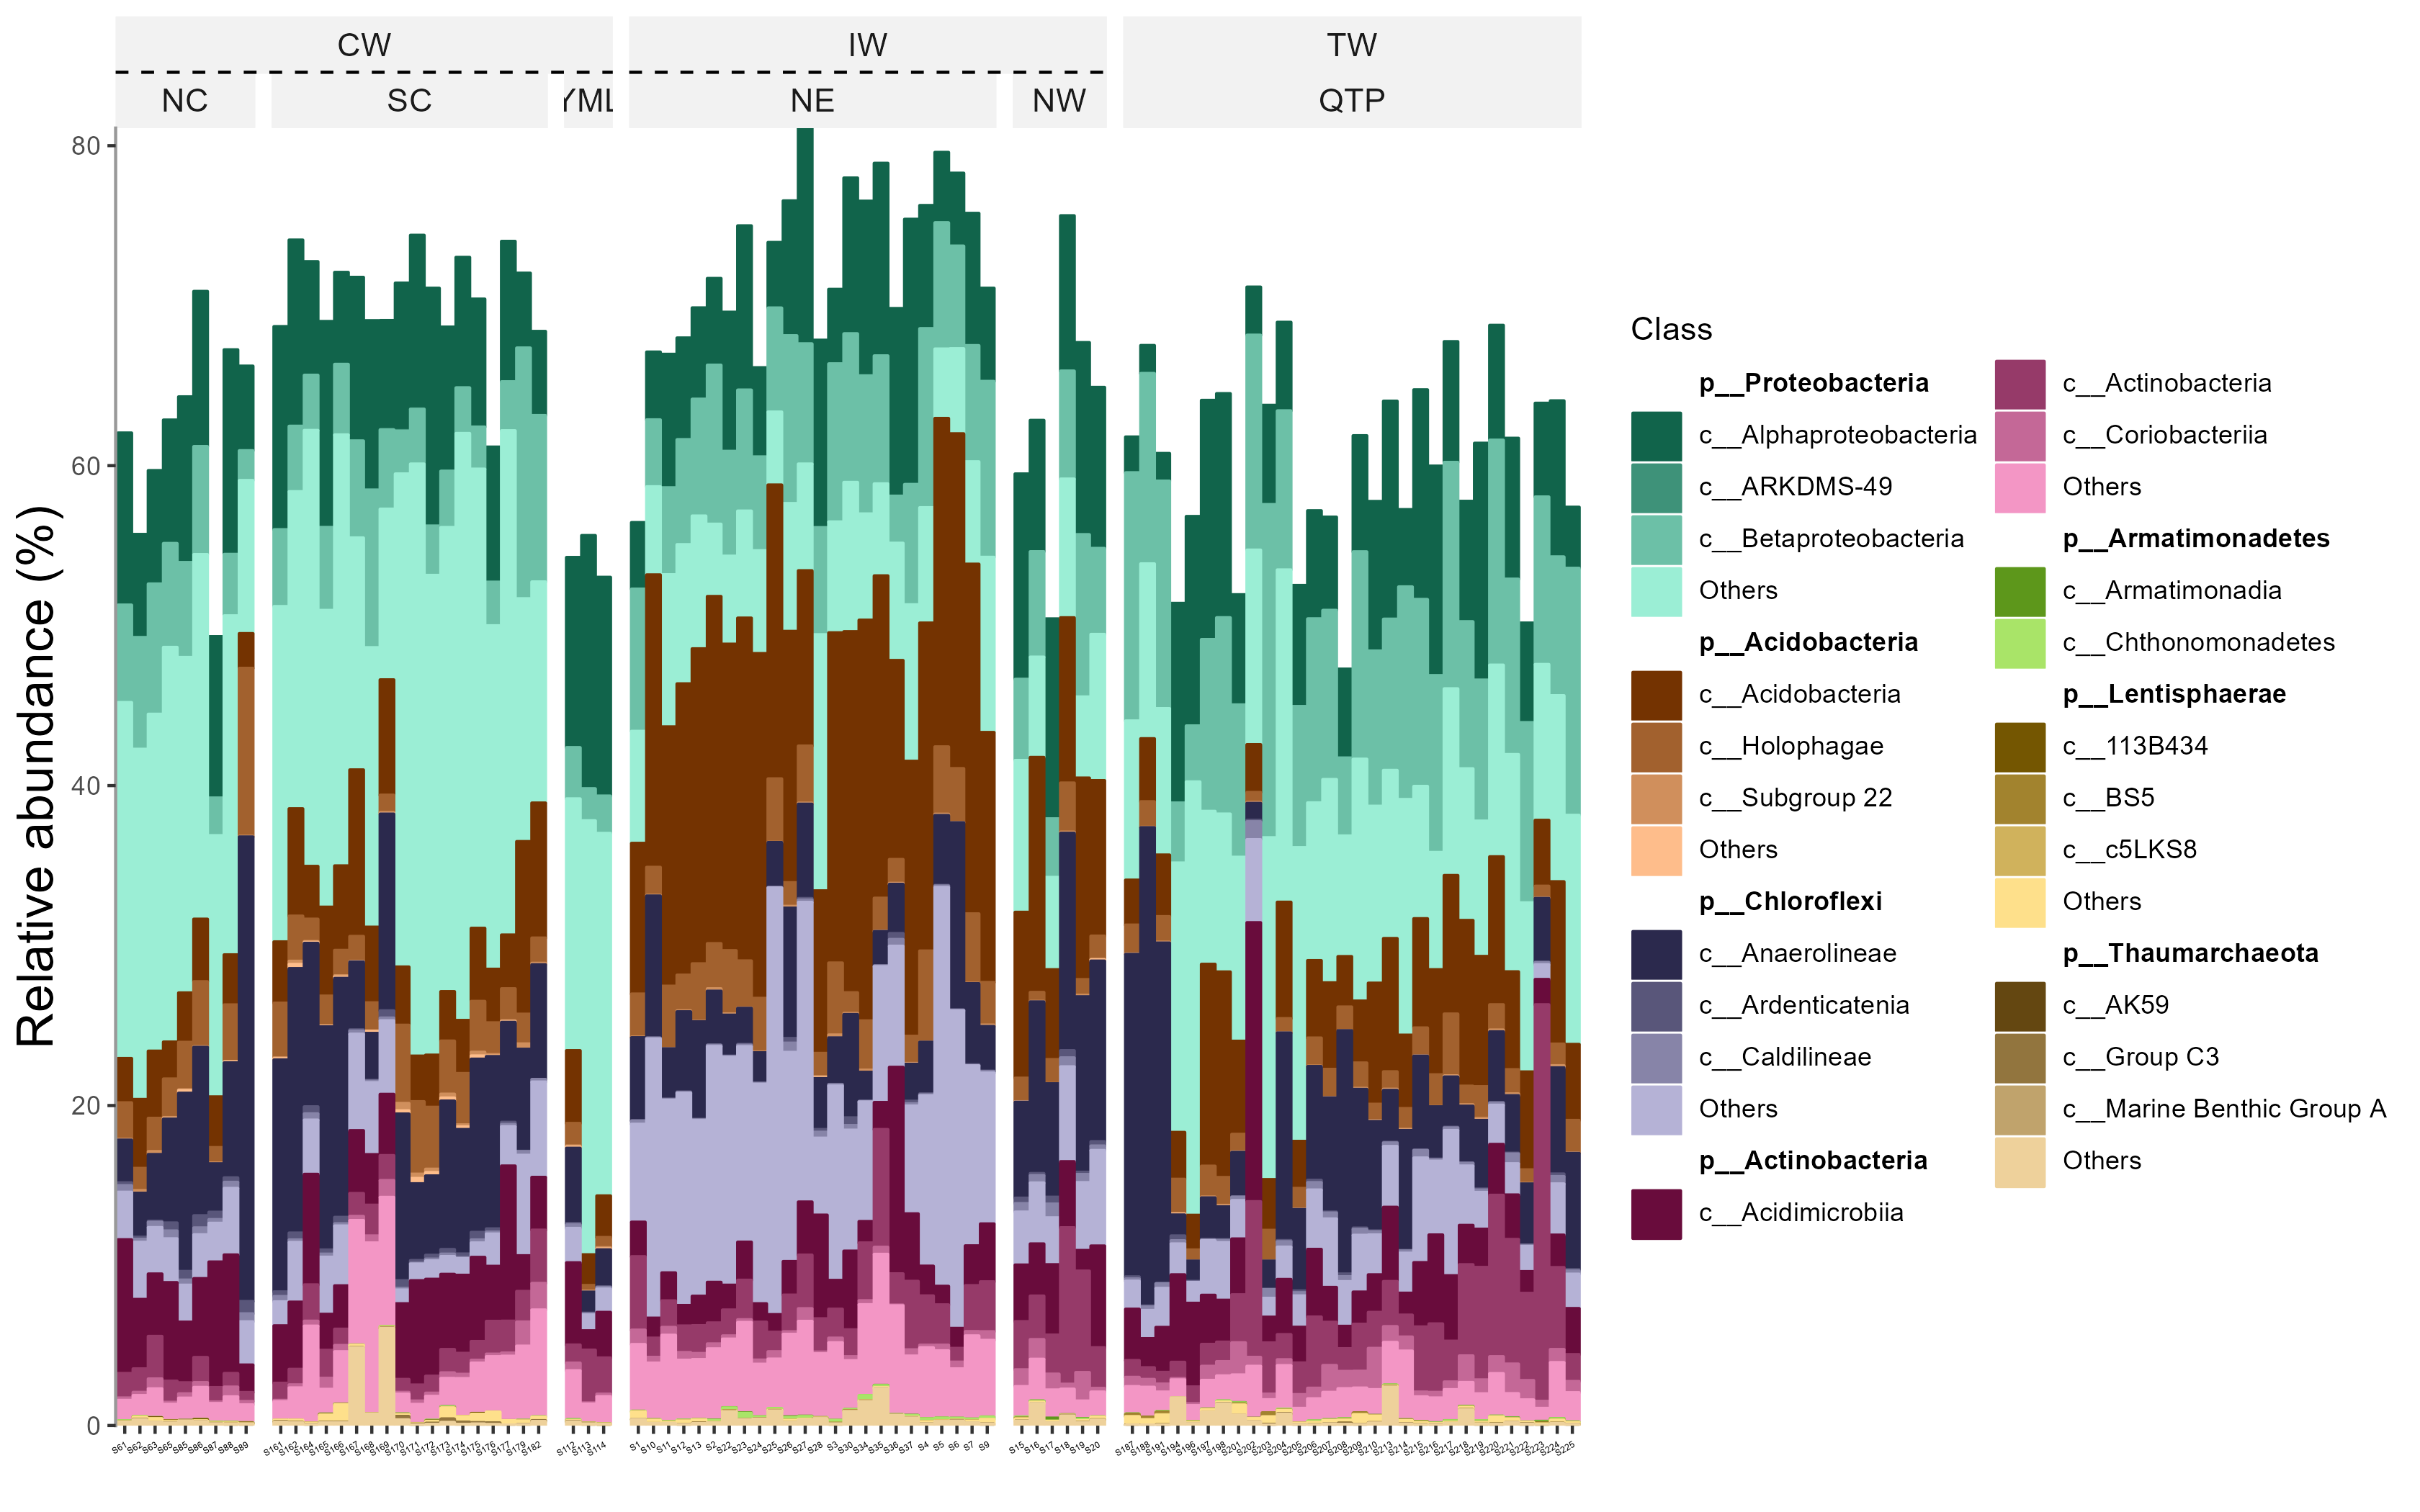
\includegraphics[width=700px]{Images/trans_abund_barplot_ggnested} \end{center}

The \texttt{coord\_flip} parameter in \texttt{plot\_bar} function can be changed to make the coordinate axis flipped.
The clustering plot can also be added in the bar plot.
In this case, the coordinate axis will be flipped automatically for better visualization.

\begin{Shaded}
\begin{Highlighting}[]
\NormalTok{t1 }\OtherTok{\textless{}{-}}\NormalTok{ trans\_abund}\SpecialCharTok{$}\FunctionTok{new}\NormalTok{(}\AttributeTok{dataset =}\NormalTok{ dataset, }\AttributeTok{taxrank =} \StringTok{"Phylum"}\NormalTok{, }\AttributeTok{ntaxa =} \DecValTok{10}\NormalTok{, }\AttributeTok{groupmean =} \StringTok{"Group"}\NormalTok{)}
\NormalTok{g1 }\OtherTok{\textless{}{-}}\NormalTok{ t1}\SpecialCharTok{$}\FunctionTok{plot\_bar}\NormalTok{(}\AttributeTok{coord\_flip =} \ConstantTok{TRUE}\NormalTok{)}
\NormalTok{g1 }\OtherTok{\textless{}{-}}\NormalTok{ g1 }\SpecialCharTok{+} \FunctionTok{theme\_classic}\NormalTok{() }\SpecialCharTok{+} \FunctionTok{theme}\NormalTok{(}\AttributeTok{axis.title.x =} \FunctionTok{element\_text}\NormalTok{(}\AttributeTok{size =} \DecValTok{16}\NormalTok{), }\AttributeTok{axis.ticks.y =} \FunctionTok{element\_blank}\NormalTok{(), }\AttributeTok{axis.line.y =} \FunctionTok{element\_blank}\NormalTok{())}
\NormalTok{g1}
\NormalTok{g1 }\OtherTok{\textless{}{-}}\NormalTok{ t1}\SpecialCharTok{$}\FunctionTok{plot\_bar}\NormalTok{(}\AttributeTok{clustering\_plot =} \ConstantTok{TRUE}\NormalTok{)}
\CommentTok{\# In this case, g1 (aplot object) is the combination of different ggplot objects}
\CommentTok{\# to adjust the main plot, please select g1[[1]]}
\NormalTok{g1[[}\DecValTok{1}\NormalTok{]] }\OtherTok{\textless{}{-}}\NormalTok{ g1[[}\DecValTok{1}\NormalTok{]] }\SpecialCharTok{+} \FunctionTok{theme\_classic}\NormalTok{() }\SpecialCharTok{+} \FunctionTok{theme}\NormalTok{(}\AttributeTok{axis.title.x =} \FunctionTok{element\_text}\NormalTok{(}\AttributeTok{size =} \DecValTok{16}\NormalTok{), }\AttributeTok{axis.ticks.y =} \FunctionTok{element\_blank}\NormalTok{(), }\AttributeTok{axis.line.y =} \FunctionTok{element\_blank}\NormalTok{())}
\NormalTok{g1}
\CommentTok{\# save the figure}
\FunctionTok{ggsave}\NormalTok{(}\StringTok{"test.png"}\NormalTok{, g1, }\AttributeTok{width =} \DecValTok{8}\NormalTok{, }\AttributeTok{height =} \DecValTok{5}\NormalTok{)}
\end{Highlighting}
\end{Shaded}

\begin{center}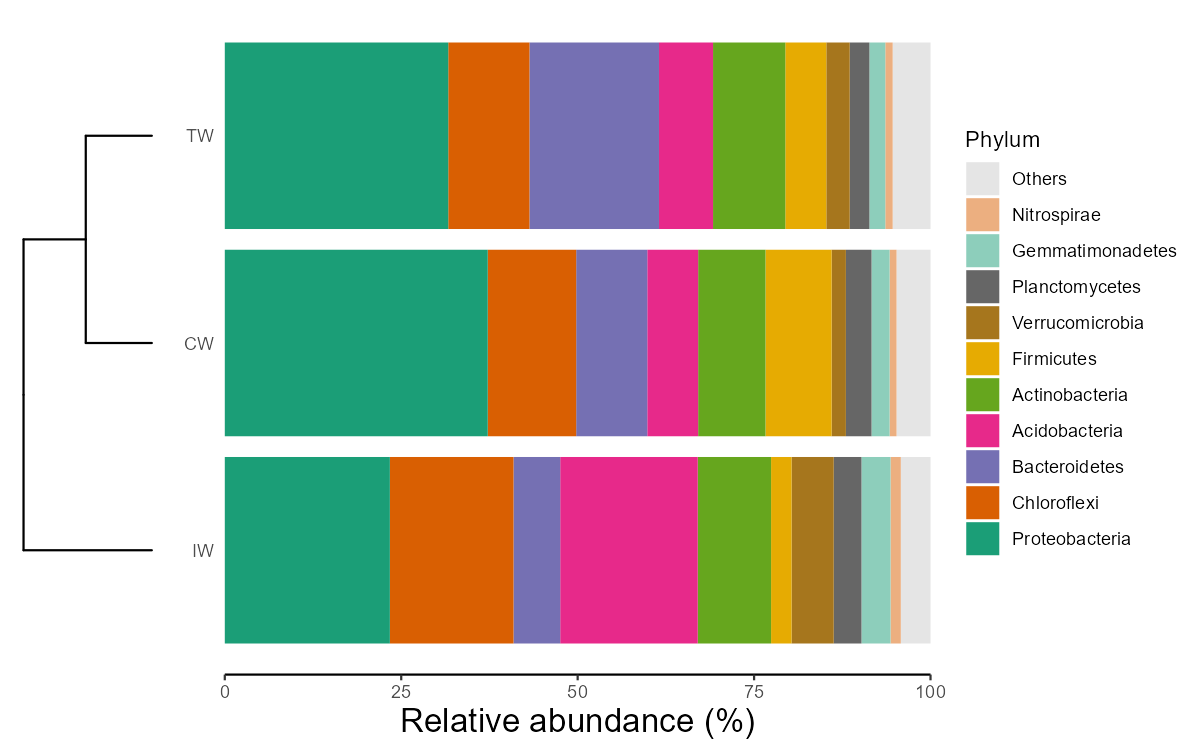
\includegraphics[width=600px]{Images/trans_abund_barplot_groupmean_clustering_flip} \end{center}

\hypertarget{key-points-1}{%
\subsection{Key points}\label{key-points-1}}

\begin{itemize}
\tightlist
\item
  trans\_abund\$new: creating trans\_abund object can invoke taxa\_abund in microtable for transformation
\item
  color\_values parameter: color\_values parameter in each function is used for colors selection
\item
  input\_taxaname parameter: input\_taxaname parameter in trans\_abund\$new can be used to select interested customized taxa instead of abundance-based selection
\item
  use\_percentage parameter: use\_percentage parameter in trans\_abund\$new - whether show the abundance percentage
\end{itemize}

\hypertarget{trans_venn-class}{%
\section{trans\_venn class}\label{trans_venn-class}}

The trans\_venn class is developed for venn analysis, i.e.~shared and unique taxa across samples/groups.

\hypertarget{example-1}{%
\subsection{Example}\label{example-1}}

This part can be performed using samples or groups at OTU/ASV level or higher taxonomic level.
To analyze the unique and shared OTUs of groups,
we first merge samples according to the ``Group'' column of sample\_table.

\begin{Shaded}
\begin{Highlighting}[]
\CommentTok{\# merge samples as one community for each group}
\NormalTok{dataset1 }\OtherTok{\textless{}{-}}\NormalTok{ dataset}\SpecialCharTok{$}\FunctionTok{merge\_samples}\NormalTok{(}\AttributeTok{use\_group =} \StringTok{"Group"}\NormalTok{)}
\CommentTok{\# dataset1 is a new microtable object}
\CommentTok{\# create trans\_venn object}
\NormalTok{t1 }\OtherTok{\textless{}{-}}\NormalTok{ trans\_venn}\SpecialCharTok{$}\FunctionTok{new}\NormalTok{(dataset1, }\AttributeTok{ratio =} \ConstantTok{NULL}\NormalTok{)}
\NormalTok{t1}\SpecialCharTok{$}\FunctionTok{plot\_venn}\NormalTok{()}
\end{Highlighting}
\end{Shaded}

\begin{center}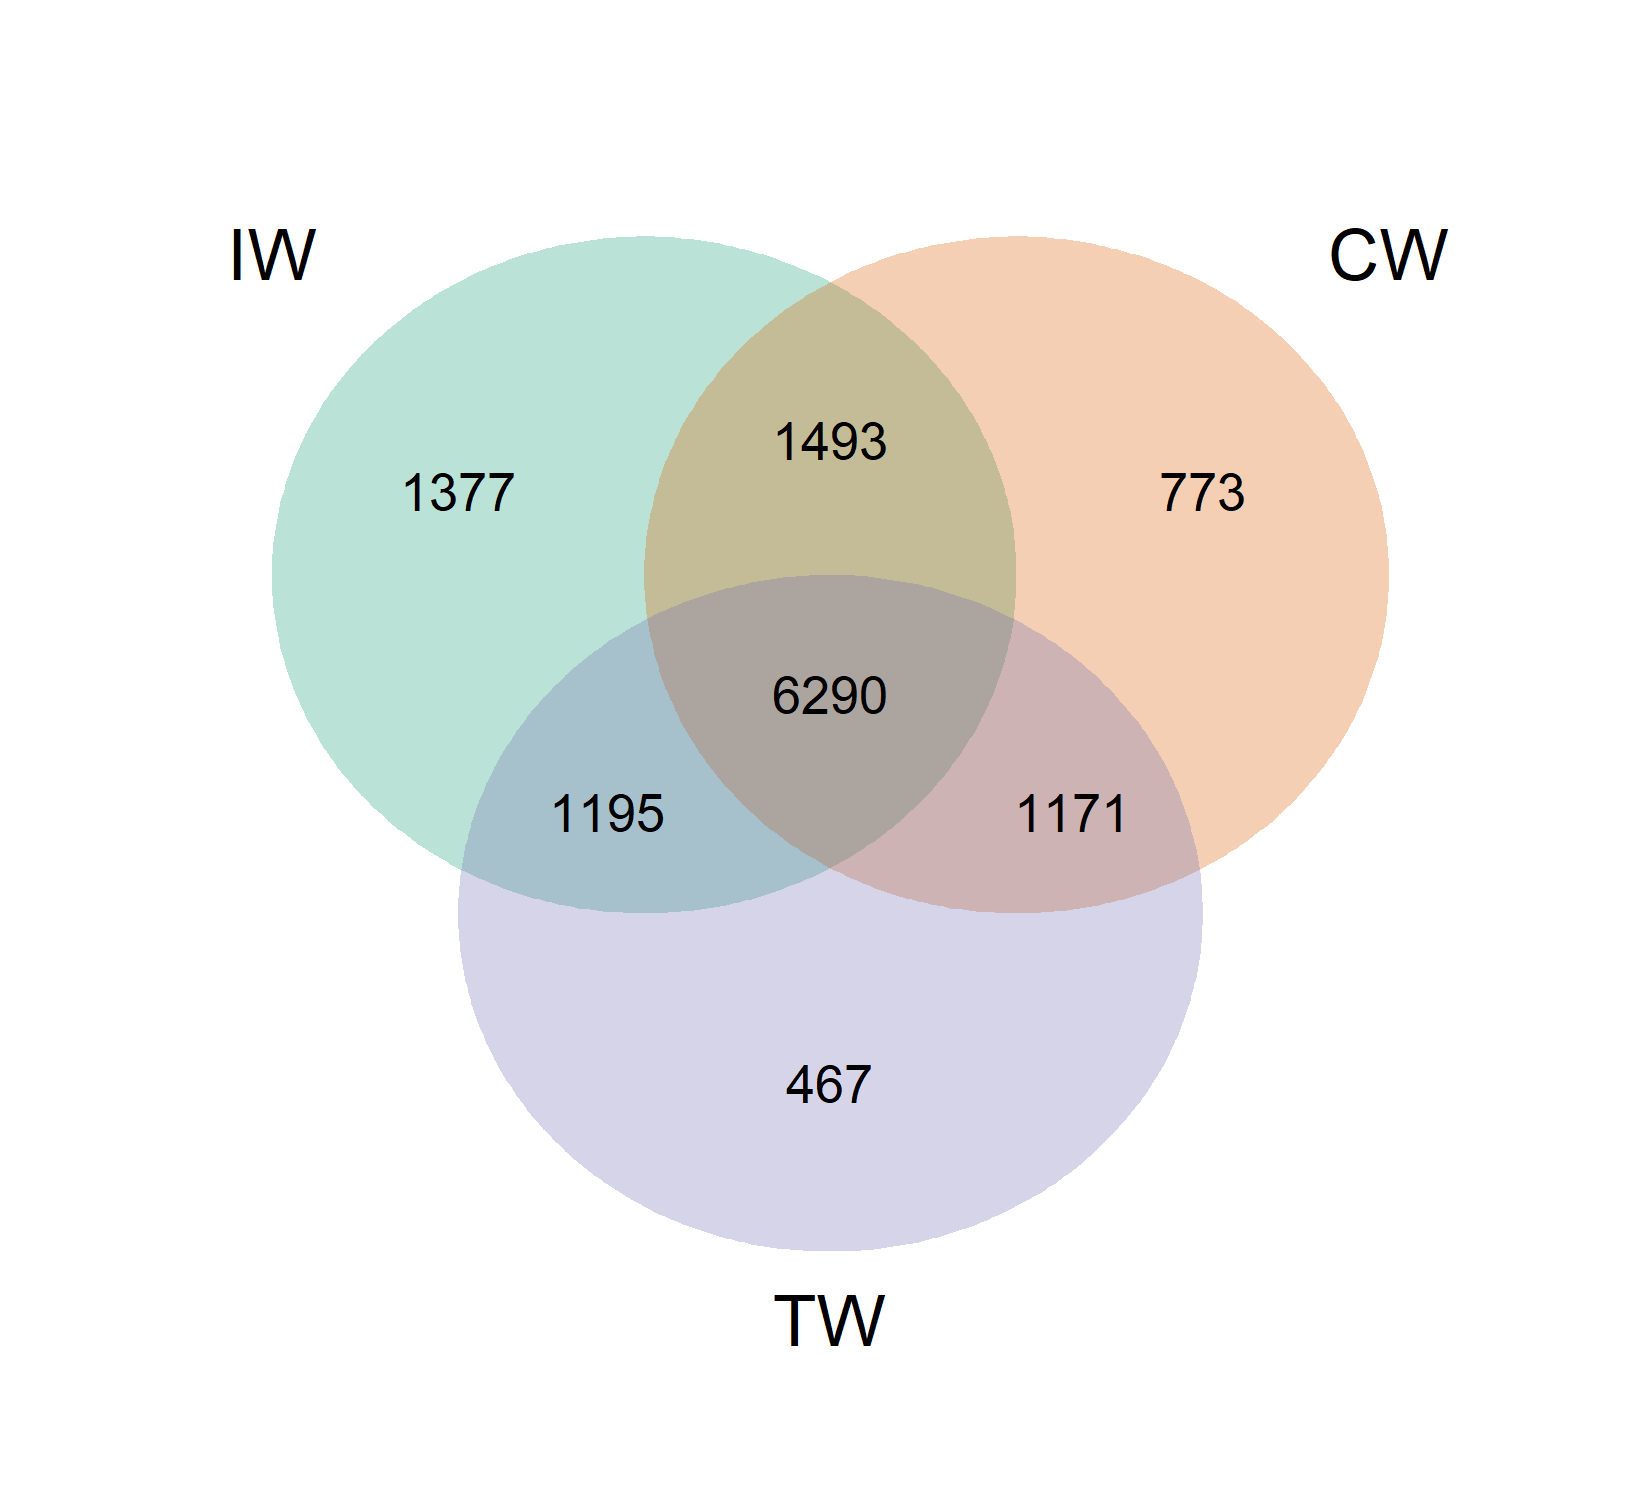
\includegraphics[width=500px]{Images/trans_venn_0} \end{center}

\begin{Shaded}
\begin{Highlighting}[]
\CommentTok{\# create venn plot with more information}
\NormalTok{t1 }\OtherTok{\textless{}{-}}\NormalTok{ trans\_venn}\SpecialCharTok{$}\FunctionTok{new}\NormalTok{(dataset1, }\AttributeTok{ratio =} \StringTok{"seqratio"}\NormalTok{)}
\NormalTok{t1}\SpecialCharTok{$}\FunctionTok{plot\_venn}\NormalTok{()}
\CommentTok{\# The integer is OTU number}
\CommentTok{\# The percentage data is the sequence number/total sequence number}
\end{Highlighting}
\end{Shaded}

\begin{center}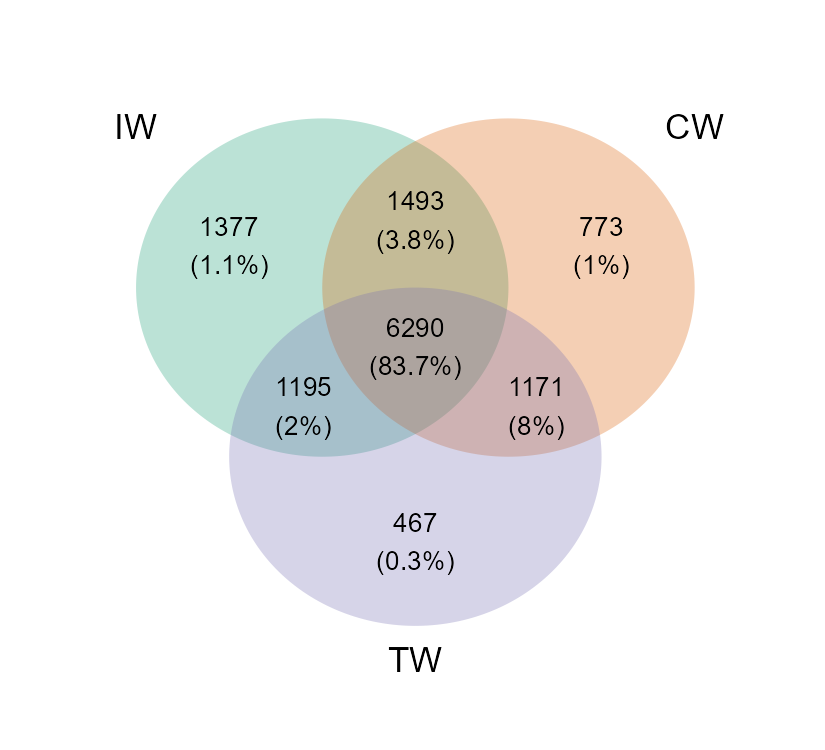
\includegraphics[width=500px]{Images/trans_venn_1} \end{center}

When the groups are too many to show with venn plot, using petal plot is better.
To assign different colors in petals, please provide multiple colors to \texttt{petal\_color} parameter.

\begin{Shaded}
\begin{Highlighting}[]
\CommentTok{\# use "Type" column in sample\_table}
\NormalTok{dataset1 }\OtherTok{\textless{}{-}}\NormalTok{ dataset}\SpecialCharTok{$}\FunctionTok{merge\_samples}\NormalTok{(}\AttributeTok{use\_group =} \StringTok{"Type"}\NormalTok{)}
\NormalTok{t1 }\OtherTok{\textless{}{-}}\NormalTok{ trans\_venn}\SpecialCharTok{$}\FunctionTok{new}\NormalTok{(dataset1)}
\NormalTok{t1}\SpecialCharTok{$}\FunctionTok{plot\_venn}\NormalTok{(}\AttributeTok{petal\_plot =} \ConstantTok{TRUE}\NormalTok{, }\AttributeTok{petal\_color =}\NormalTok{ RColorBrewer}\SpecialCharTok{::}\FunctionTok{brewer.pal}\NormalTok{(}\DecValTok{8}\NormalTok{, }\StringTok{"Dark2"}\NormalTok{))}
\NormalTok{t1}\SpecialCharTok{$}\FunctionTok{plot\_venn}\NormalTok{(}\AttributeTok{petal\_plot =} \ConstantTok{TRUE}\NormalTok{, }\AttributeTok{petal\_center\_size =} \DecValTok{50}\NormalTok{, }\AttributeTok{petal\_r =} \FloatTok{1.5}\NormalTok{, }\AttributeTok{petal\_a =} \DecValTok{3}\NormalTok{, }\AttributeTok{petal\_move\_xy =} \FloatTok{3.8}\NormalTok{, }\AttributeTok{petal\_color\_center =} \StringTok{"\#BEBADA"}\NormalTok{)}
\end{Highlighting}
\end{Shaded}

\begin{center}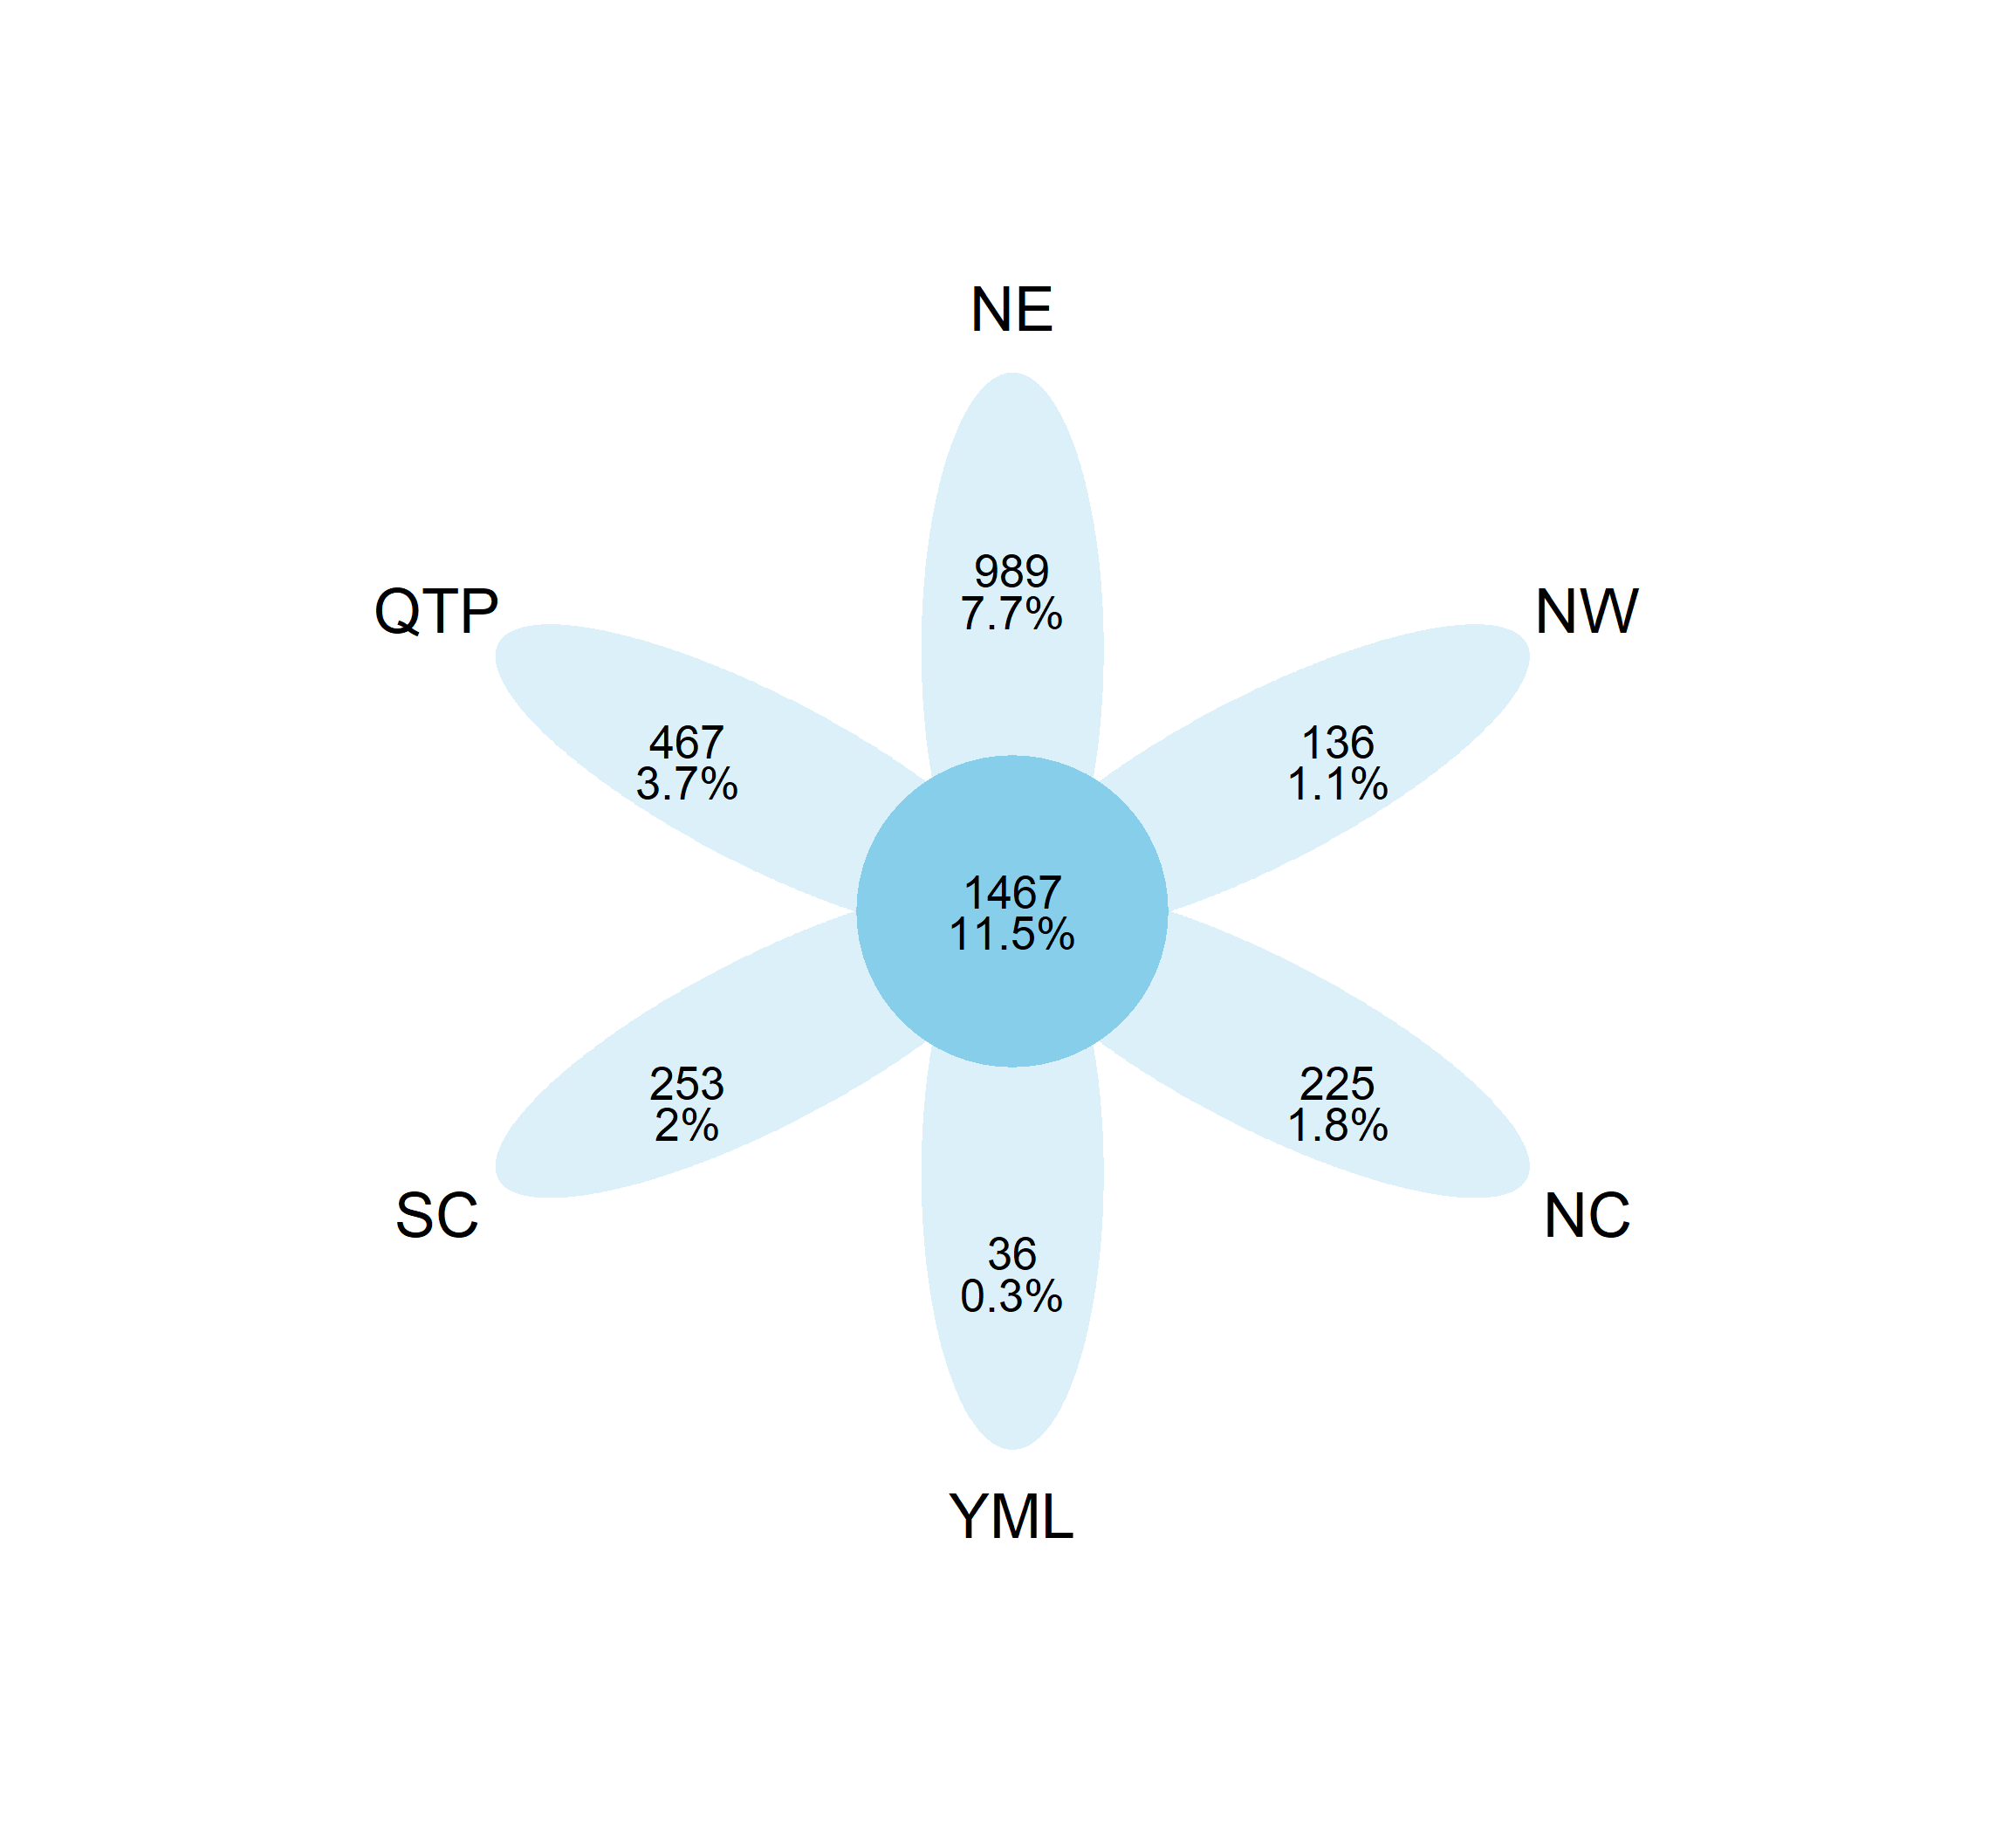
\includegraphics[width=500px]{Images/trans_venn_2} \end{center}

Another way to plot the results is to use \texttt{plot\_bar} function, which is especially useful for a large number of samples/groups.
This way is generally called UpSet plot. Please see the help document for more parameters to adjust the plot.

\begin{Shaded}
\begin{Highlighting}[]
\NormalTok{tmp }\OtherTok{\textless{}{-}}\NormalTok{ dataset}\SpecialCharTok{$}\FunctionTok{merge\_samples}\NormalTok{(}\AttributeTok{use\_group =} \StringTok{"Type"}\NormalTok{)}
\NormalTok{tmp}
\NormalTok{t1 }\OtherTok{\textless{}{-}}\NormalTok{ trans\_venn}\SpecialCharTok{$}\FunctionTok{new}\NormalTok{(}\AttributeTok{dataset =}\NormalTok{ tmp)}
\CommentTok{\# only show some sets with large intersection numbers}
\NormalTok{t1}\SpecialCharTok{$}\NormalTok{data\_summary }\SpecialCharTok{\%\textless{}\textgreater{}\%}\NormalTok{ .[.[, }\DecValTok{1}\NormalTok{] }\SpecialCharTok{\textgreater{}} \DecValTok{20}\NormalTok{, ]}
\NormalTok{g1 }\OtherTok{\textless{}{-}}\NormalTok{ t1}\SpecialCharTok{$}\FunctionTok{plot\_bar}\NormalTok{(}\AttributeTok{left\_plot =} \ConstantTok{TRUE}\NormalTok{, }\AttributeTok{bottom\_height =} \FloatTok{0.5}\NormalTok{, }\AttributeTok{left\_width =} \FloatTok{0.15}\NormalTok{, }\AttributeTok{up\_bar\_fill =} \StringTok{"grey50"}\NormalTok{, }\AttributeTok{left\_bar\_fill =} \StringTok{"grey50"}\NormalTok{, }\AttributeTok{bottom\_point\_color =} \StringTok{"black"}\NormalTok{)}
\NormalTok{g1}
\CommentTok{\# g1 is aplot class and can be saved with ggplot2::ggsave, aplot::ggsave or cowplot::save\_plot function}
\CommentTok{\# as g1 is comprised of several sub{-}plots, please adjust the details for each sub{-}plot}
\NormalTok{g1[[}\DecValTok{1}\NormalTok{]]}
\NormalTok{g1[[}\DecValTok{2}\NormalTok{]]}
\end{Highlighting}
\end{Shaded}

\begin{center}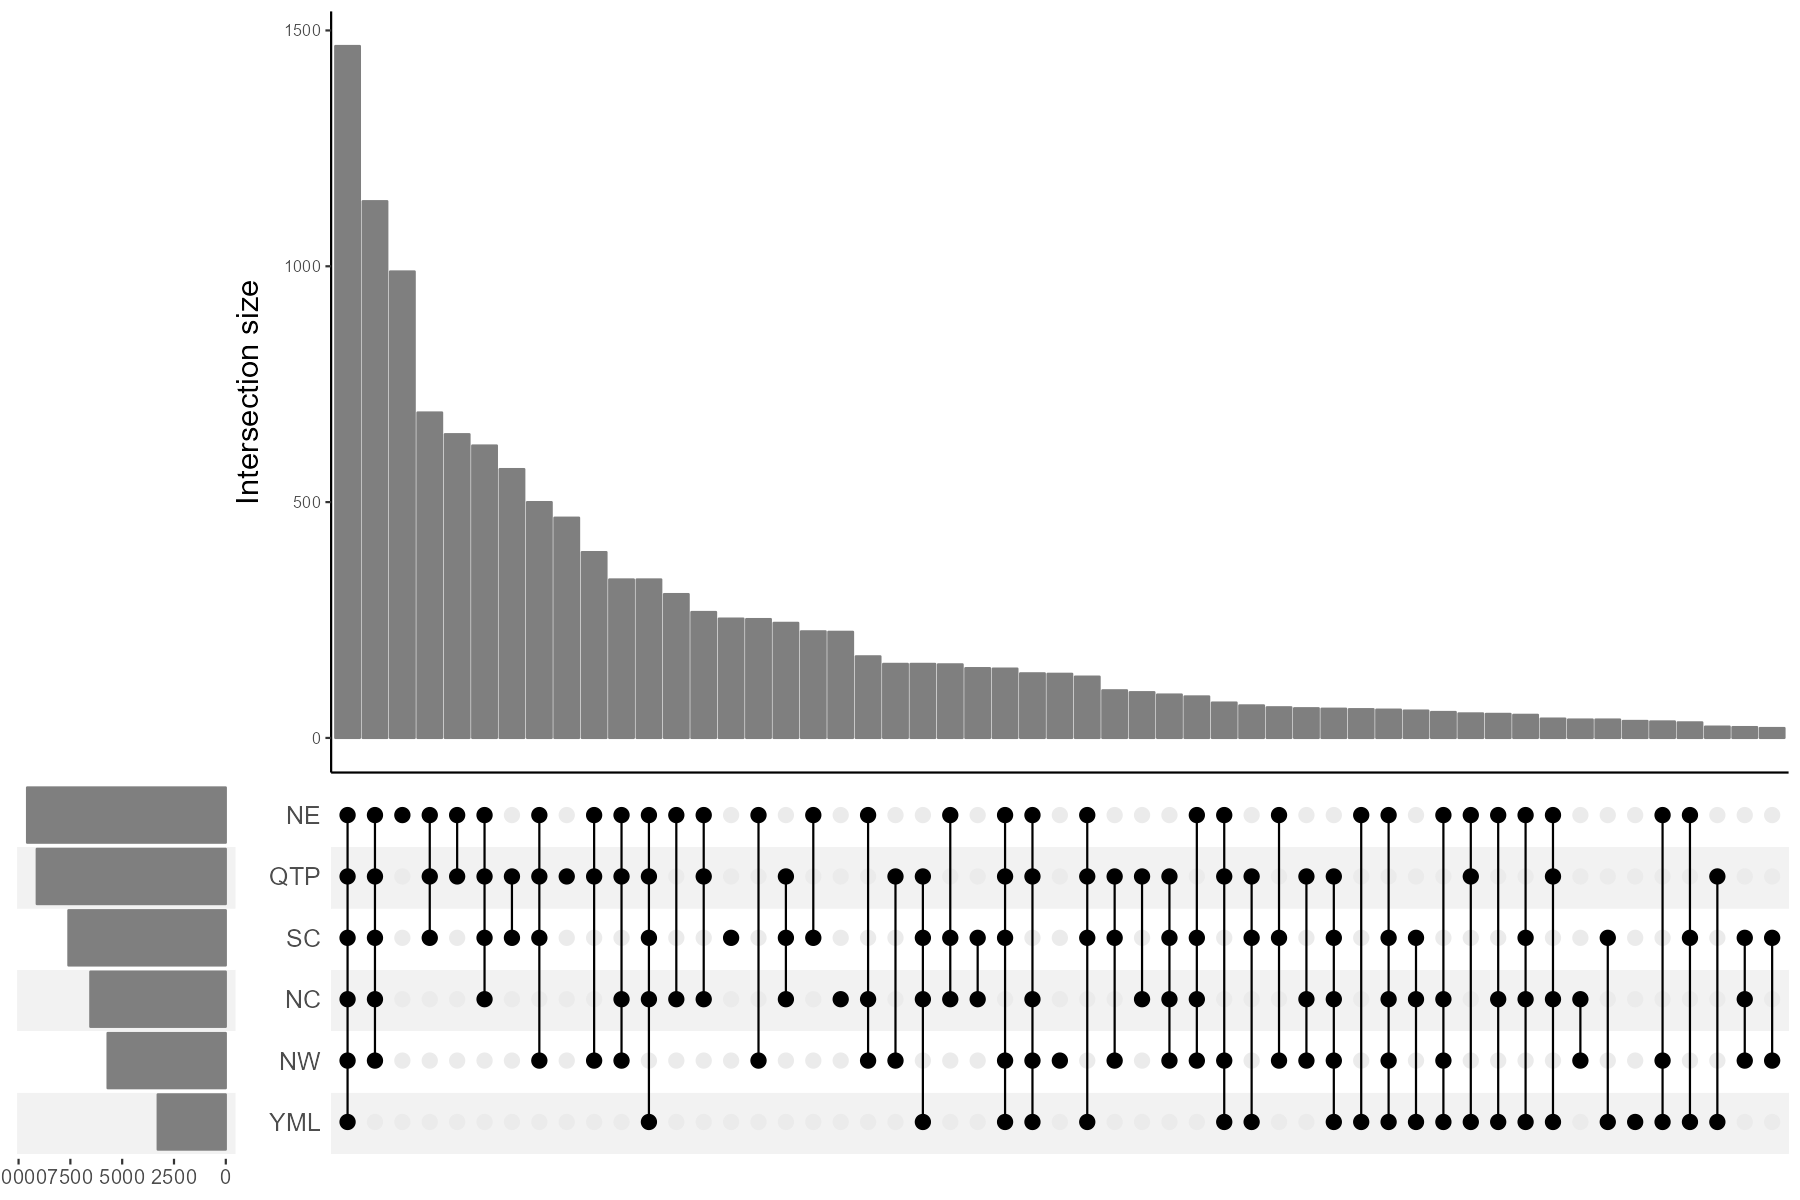
\includegraphics[width=800px]{Images/trans_venn_3} \end{center}

Generally, after getting the intersection results, we do not know who those shared or unique taxa are.
The composition of the unique or shared species may account for the different and similar parts of ecological characteristics across groups\citep{Mendes_Deciphering_2011}.
So, it is interesting to further analyze the composition of unique and shared species.
For this goal, we first transform the results of venn plot to the traditional feature-sample table, that is, another object of microtable class.

\begin{Shaded}
\begin{Highlighting}[]
\NormalTok{dataset1 }\OtherTok{\textless{}{-}}\NormalTok{ dataset}\SpecialCharTok{$}\FunctionTok{merge\_samples}\NormalTok{(}\AttributeTok{use\_group =} \StringTok{"Group"}\NormalTok{)}
\NormalTok{t1 }\OtherTok{\textless{}{-}}\NormalTok{ trans\_venn}\SpecialCharTok{$}\FunctionTok{new}\NormalTok{(dataset1)}
\end{Highlighting}
\end{Shaded}

\begin{verbatim}
## The details of each venn part is stored in object$data_details ...
\end{verbatim}

\begin{verbatim}
## The venn summary table used for plot is stored in object$data_summary ...
\end{verbatim}

\begin{Shaded}
\begin{Highlighting}[]
\CommentTok{\# transform venn results to the sample{-}species table, here do not consider abundance, only use presence/absence.}
\NormalTok{t2 }\OtherTok{\textless{}{-}}\NormalTok{ t1}\SpecialCharTok{$}\FunctionTok{trans\_comm}\NormalTok{(}\AttributeTok{use\_frequency =} \ConstantTok{TRUE}\NormalTok{)}
\CommentTok{\# t2 is a new microtable class, each part is considered a sample}
\FunctionTok{class}\NormalTok{(t2)}
\end{Highlighting}
\end{Shaded}

\begin{verbatim}
## [1] "microtable" "R6"
\end{verbatim}

We use bar plot to show the composition at the Genus level.

\begin{Shaded}
\begin{Highlighting}[]
\CommentTok{\# calculate taxa abundance, that is, the frequency}
\NormalTok{t2}\SpecialCharTok{$}\FunctionTok{cal\_abund}\NormalTok{()}
\CommentTok{\# transform and plot}
\NormalTok{t3 }\OtherTok{\textless{}{-}}\NormalTok{ trans\_abund}\SpecialCharTok{$}\FunctionTok{new}\NormalTok{(}\AttributeTok{dataset =}\NormalTok{ t2, }\AttributeTok{taxrank =} \StringTok{"Genus"}\NormalTok{, }\AttributeTok{ntaxa =} \DecValTok{8}\NormalTok{)}
\NormalTok{t3}\SpecialCharTok{$}\FunctionTok{plot\_bar}\NormalTok{(}\AttributeTok{bar\_type =} \StringTok{"part"}\NormalTok{, }\AttributeTok{legend\_text\_italic =}\NormalTok{ T, }\AttributeTok{xtext\_angle =} \DecValTok{30}\NormalTok{, }\AttributeTok{color\_values =}\NormalTok{ RColorBrewer}\SpecialCharTok{::}\FunctionTok{brewer.pal}\NormalTok{(}\DecValTok{8}\NormalTok{, }\StringTok{"Set2"}\NormalTok{),}
    \AttributeTok{order\_x =} \FunctionTok{c}\NormalTok{(}\StringTok{"IW"}\NormalTok{, }\StringTok{"CW"}\NormalTok{, }\StringTok{"TW"}\NormalTok{, }\StringTok{"IW\&CW"}\NormalTok{, }\StringTok{"IW\&TW"}\NormalTok{, }\StringTok{"CW\&TW"}\NormalTok{, }\StringTok{"IW\&CW\&TW"}\NormalTok{)) }\SpecialCharTok{+} \FunctionTok{ylab}\NormalTok{(}\StringTok{"Frequency (\%)"}\NormalTok{)}
\end{Highlighting}
\end{Shaded}

\begin{center}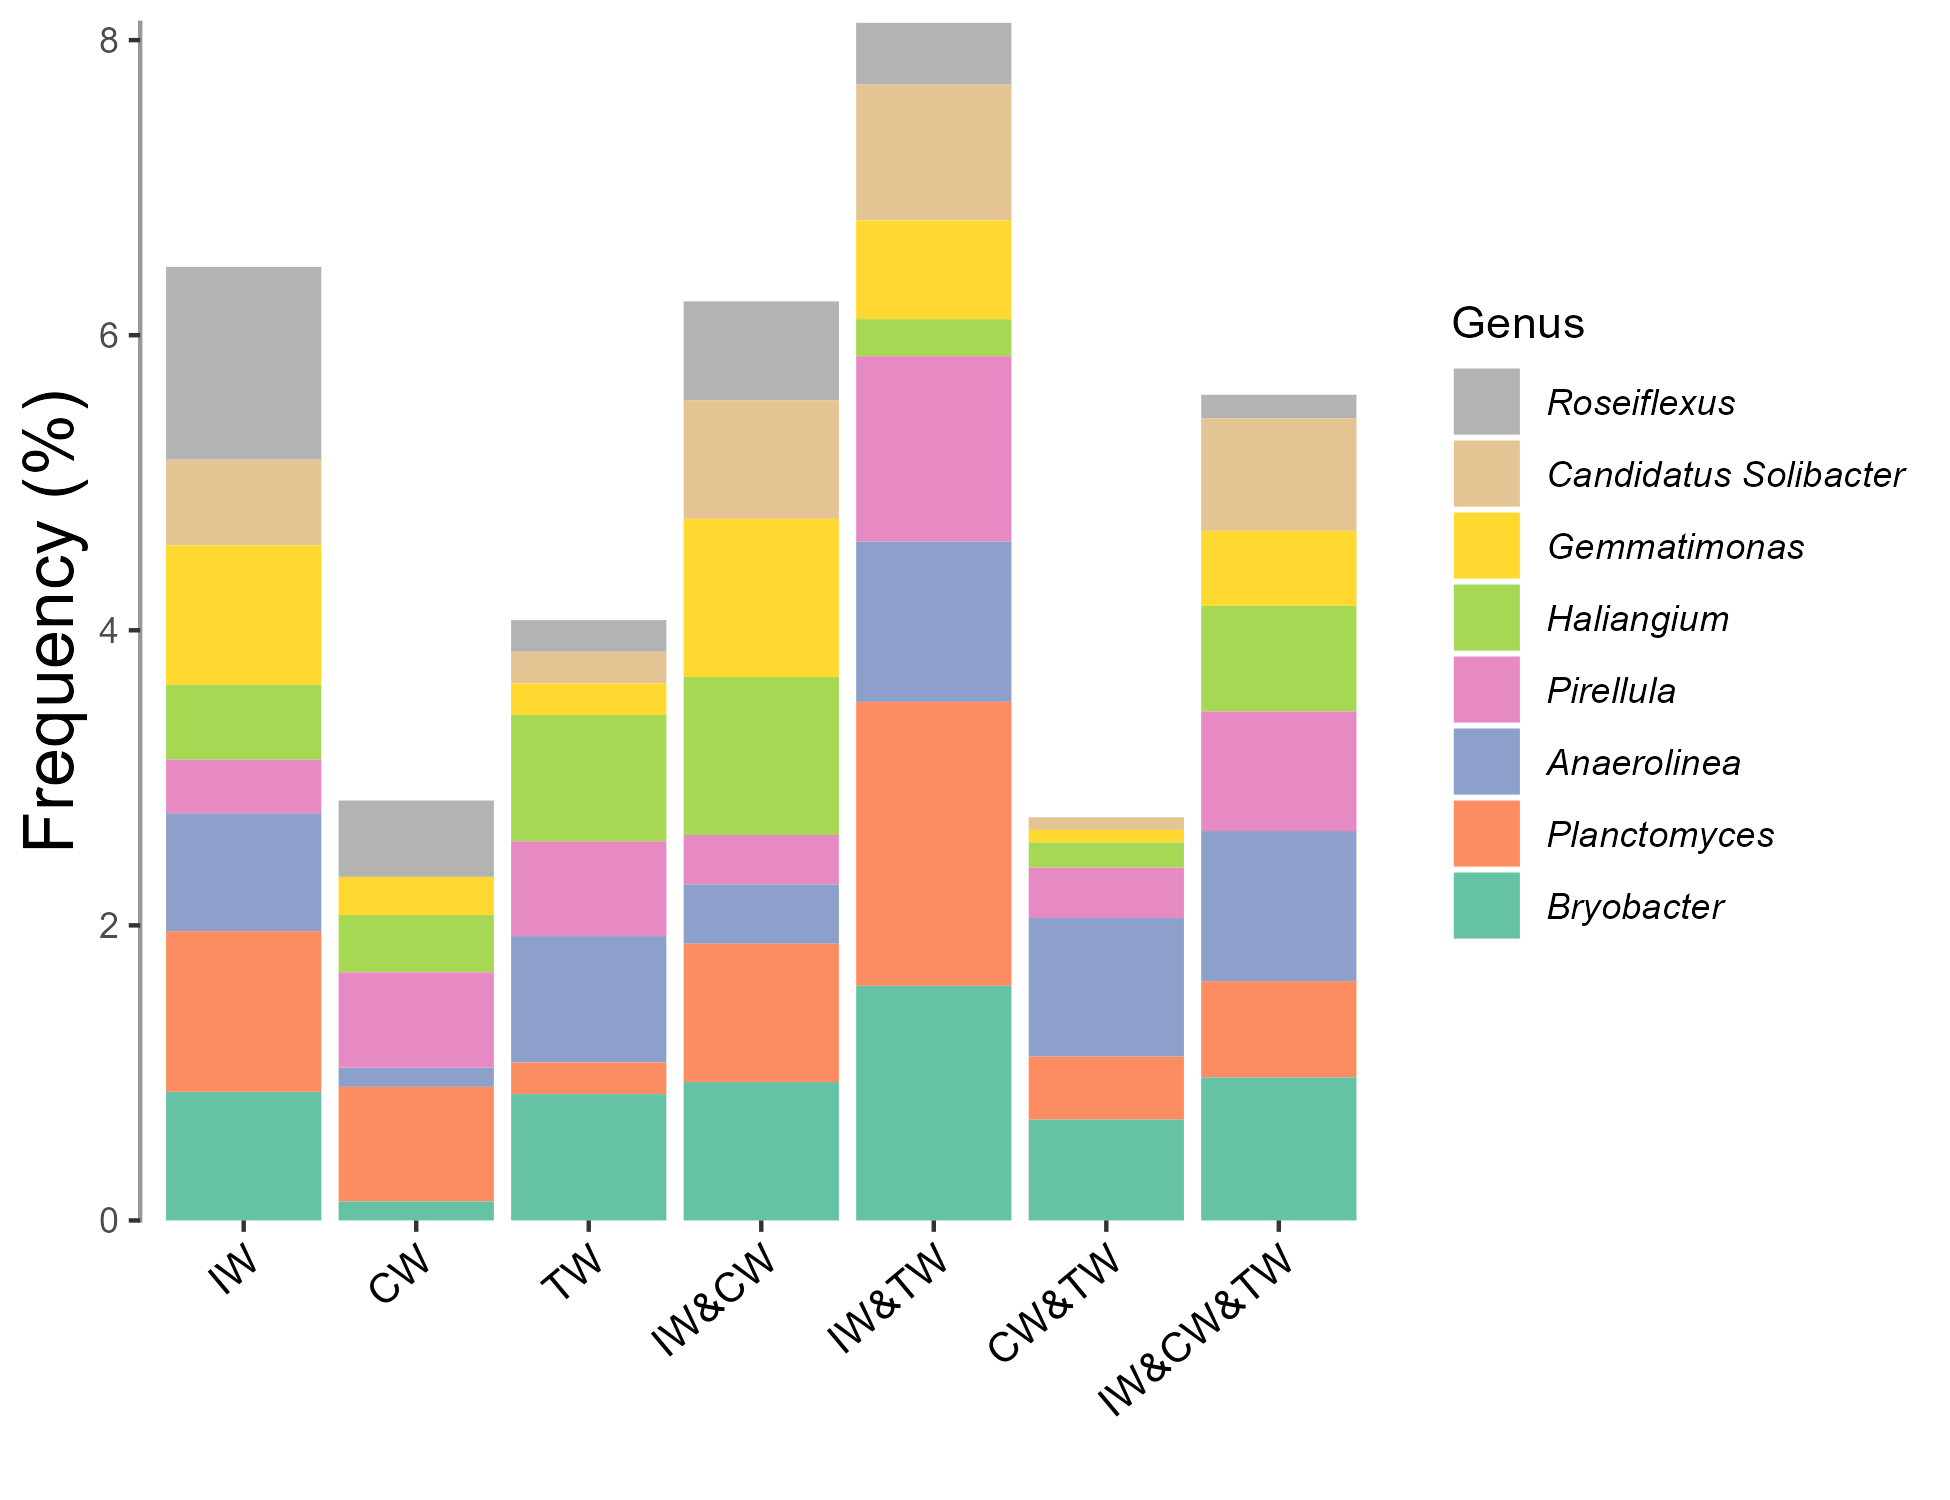
\includegraphics[width=650px]{Images/trans_venn_bar} \end{center}

We also try to use pie chart to show the compositions at the Phylum level.

\begin{Shaded}
\begin{Highlighting}[]
\NormalTok{t3 }\OtherTok{\textless{}{-}}\NormalTok{ trans\_abund}\SpecialCharTok{$}\FunctionTok{new}\NormalTok{(}\AttributeTok{dataset =}\NormalTok{ t2, }\AttributeTok{taxrank =} \StringTok{"Phylum"}\NormalTok{, }\AttributeTok{ntaxa =} \DecValTok{8}\NormalTok{)}
\NormalTok{t3}\SpecialCharTok{$}\NormalTok{data\_abund}\SpecialCharTok{$}\NormalTok{Sample }\SpecialCharTok{\%\textless{}\textgreater{}\%} \FunctionTok{factor}\NormalTok{(., }\AttributeTok{levels =} \FunctionTok{unique}\NormalTok{(.))}
\NormalTok{t3}\SpecialCharTok{$}\FunctionTok{plot\_pie}\NormalTok{(}\AttributeTok{facet\_nrow =} \DecValTok{3}\NormalTok{, }\AttributeTok{color\_values =} \FunctionTok{c}\NormalTok{(RColorBrewer}\SpecialCharTok{::}\FunctionTok{brewer.pal}\NormalTok{(}\DecValTok{8}\NormalTok{, }\StringTok{"Dark2"}\NormalTok{), }\StringTok{"grey50"}\NormalTok{))}
\end{Highlighting}
\end{Shaded}

\begin{center}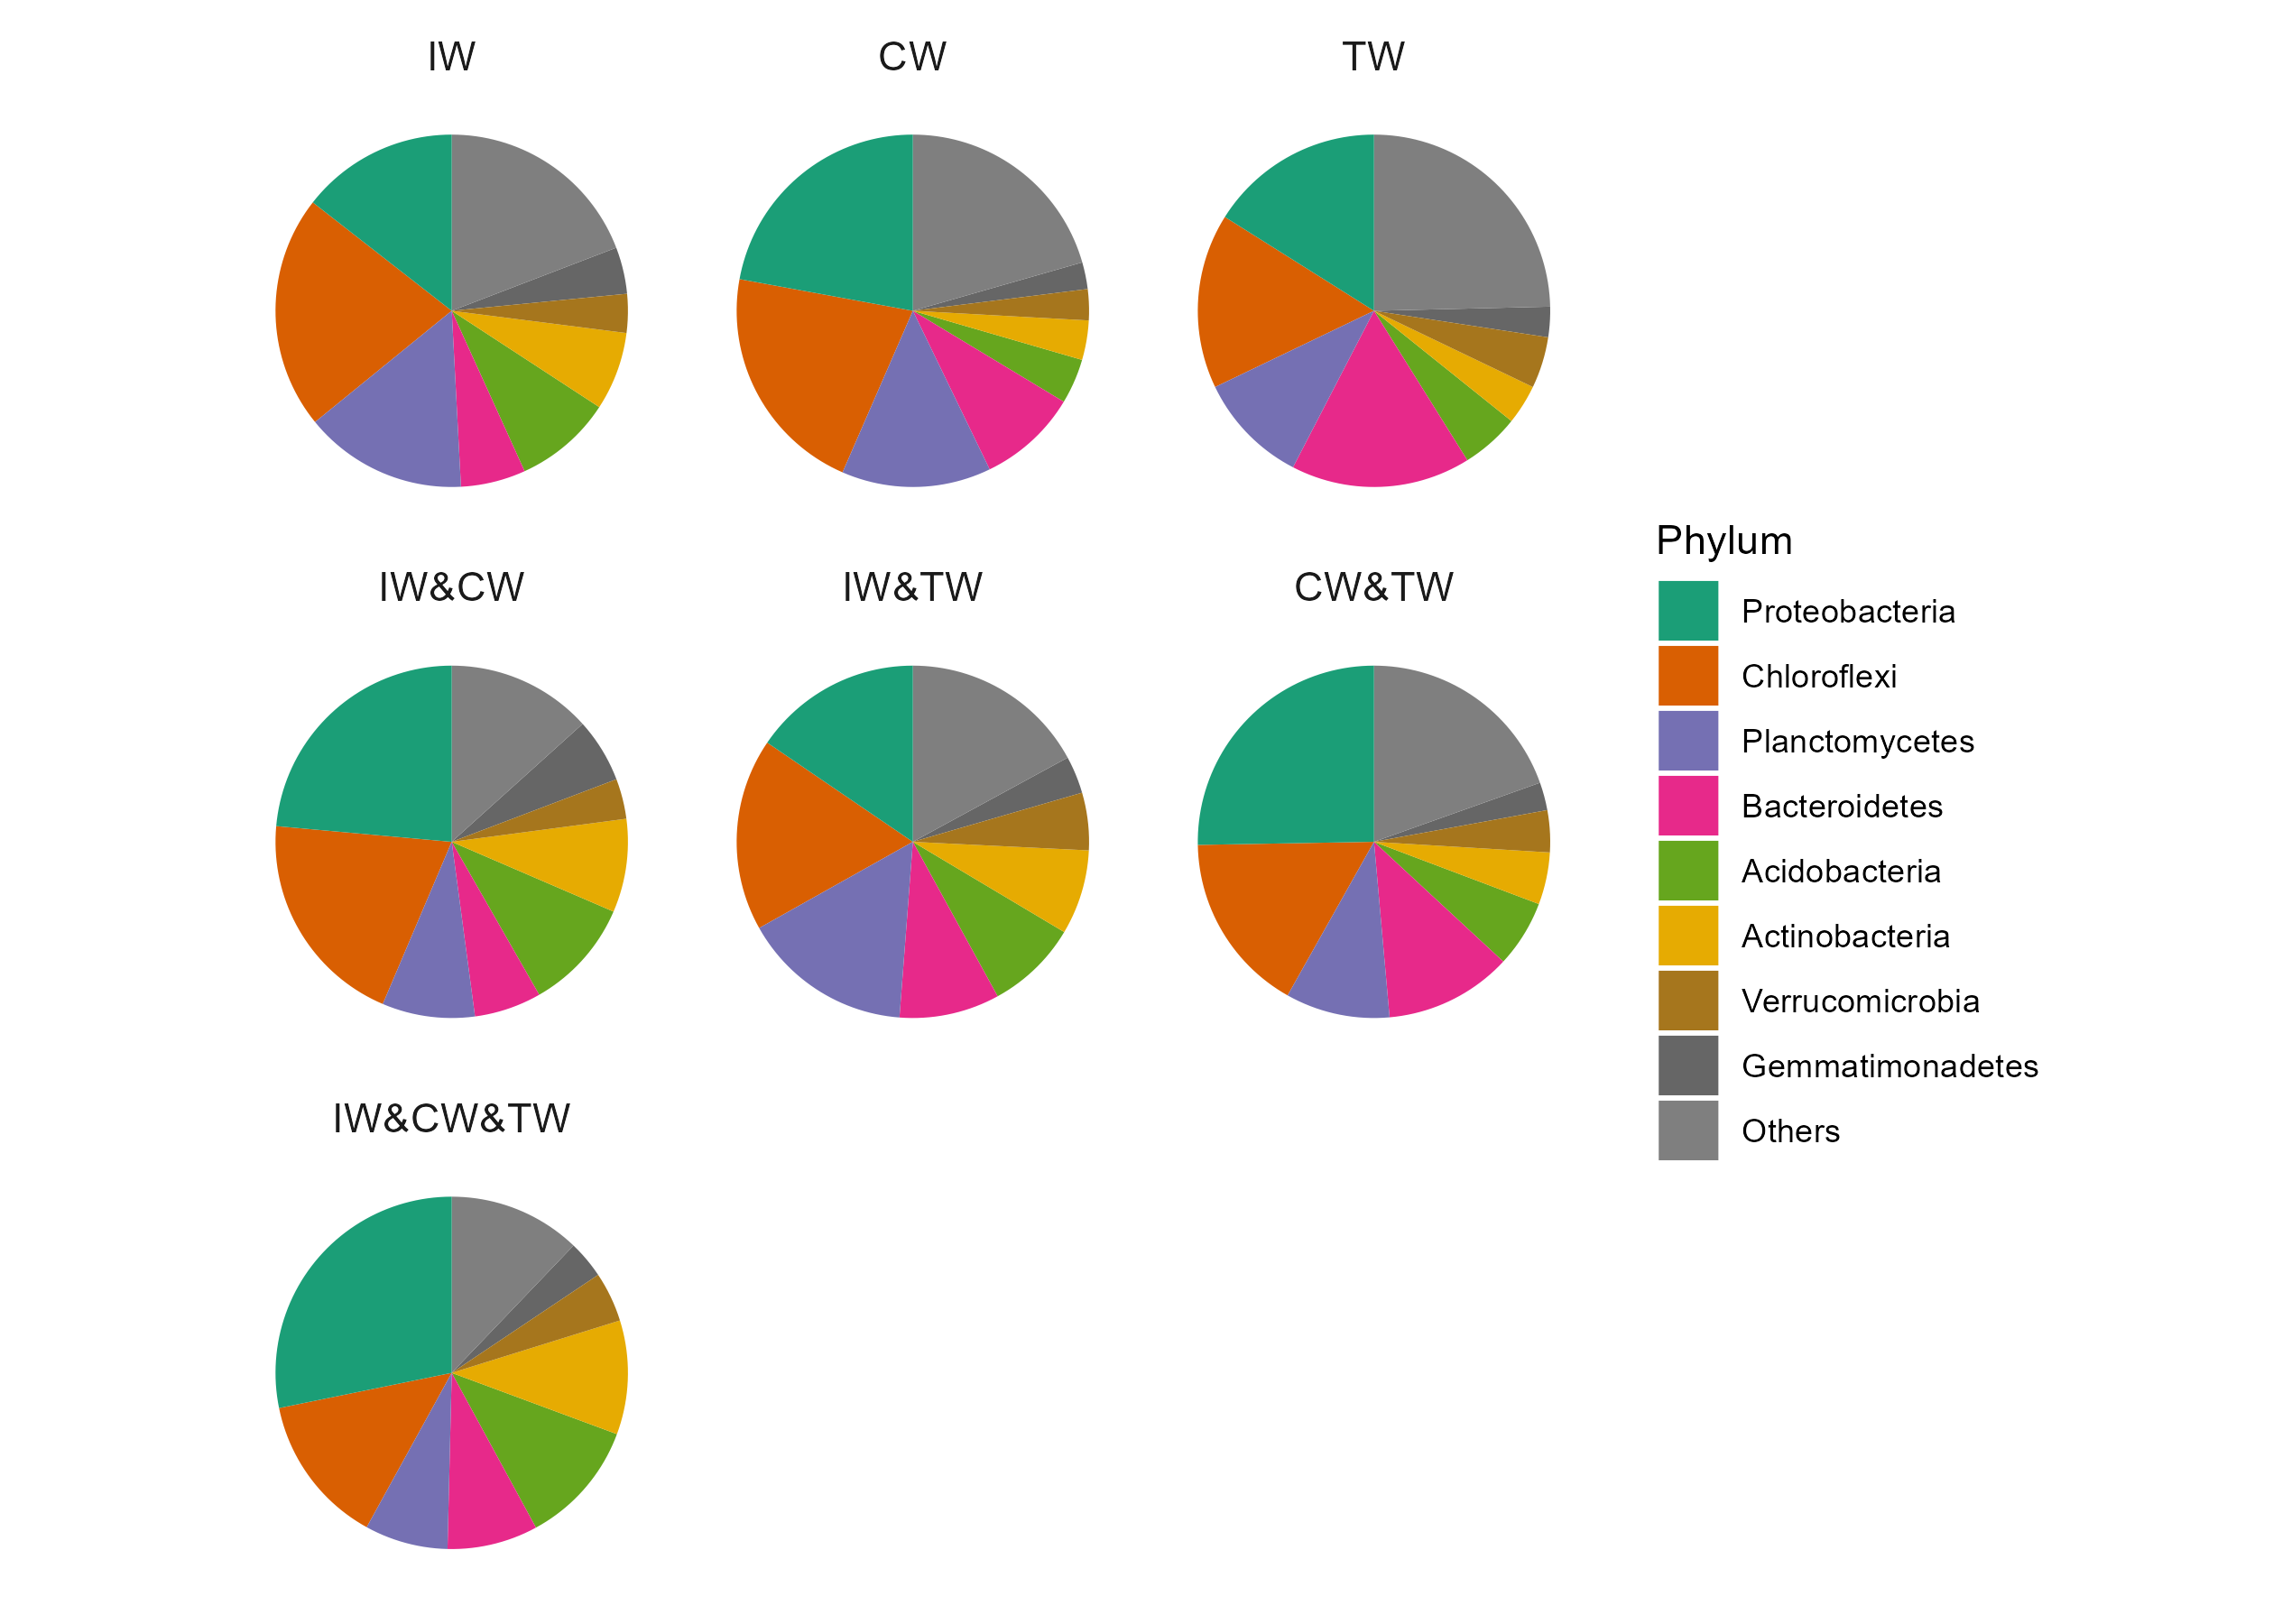
\includegraphics[width=800px]{Images/trans_venn_pie} \end{center}

Other examples:

To reorder samples in the plots, please manipulate the sample\_table in the object to adjust the orders.

\begin{Shaded}
\begin{Highlighting}[]
\NormalTok{test }\OtherTok{\textless{}{-}}\NormalTok{ dataset}\SpecialCharTok{$}\FunctionTok{merge\_samples}\NormalTok{(}\AttributeTok{use\_group =} \StringTok{"Type"}\NormalTok{)}
\NormalTok{test}\SpecialCharTok{$}\NormalTok{sample\_table }\SpecialCharTok{\%\textless{}\textgreater{}\%}\NormalTok{ .[}\FunctionTok{c}\NormalTok{(}\StringTok{"YML"}\NormalTok{, }\StringTok{"NE"}\NormalTok{, }\StringTok{"NW"}\NormalTok{, }\StringTok{"NC"}\NormalTok{, }\StringTok{"QTP"}\NormalTok{, }\StringTok{"SC"}\NormalTok{), , drop }\OtherTok{=} \ConstantTok{FALSE}\NormalTok{]}
\NormalTok{test}\SpecialCharTok{$}\FunctionTok{tidy\_dataset}\NormalTok{()}
\CommentTok{\# The columns of otu\_table can also be reordered according to the sample\_table after running tidy\_dataset function}
\NormalTok{t1 }\OtherTok{\textless{}{-}}\NormalTok{ trans\_venn}\SpecialCharTok{$}\FunctionTok{new}\NormalTok{(test)}
\NormalTok{t1}\SpecialCharTok{$}\FunctionTok{plot\_bar}\NormalTok{(}\AttributeTok{sort\_samples =} \ConstantTok{FALSE}\NormalTok{)}
\end{Highlighting}
\end{Shaded}

The parameter \texttt{sort\_samples\ =\ TRUE} in \texttt{plot\_bar} function can be applied to sort samples in the y axis according to the number of features.
The left bar plot can be removed when the parameter \texttt{left\_plot\ =\ FALSE}.

\begin{Shaded}
\begin{Highlighting}[]
\NormalTok{test }\OtherTok{\textless{}{-}}\NormalTok{ dataset}\SpecialCharTok{$}\FunctionTok{merge\_samples}\NormalTok{(}\AttributeTok{use\_group =} \StringTok{"Type"}\NormalTok{)}
\NormalTok{t1 }\OtherTok{\textless{}{-}}\NormalTok{ trans\_venn}\SpecialCharTok{$}\FunctionTok{new}\NormalTok{(test)}
\CommentTok{\# remove left bar in the UpSet plot}
\NormalTok{t1}\SpecialCharTok{$}\FunctionTok{plot\_bar}\NormalTok{(}\AttributeTok{left\_plot =} \ConstantTok{FALSE}\NormalTok{)}
\CommentTok{\# sort samples in the axis according to the number of features}
\NormalTok{t1}\SpecialCharTok{$}\FunctionTok{plot\_bar}\NormalTok{(}\AttributeTok{sort\_samples =} \ConstantTok{TRUE}\NormalTok{)}
\CommentTok{\# original orders in test$sample\_table}
\NormalTok{t1}\SpecialCharTok{$}\FunctionTok{plot\_bar}\NormalTok{(}\AttributeTok{sort\_samples =} \ConstantTok{FALSE}\NormalTok{)}
\end{Highlighting}
\end{Shaded}

\hypertarget{key-points-2}{%
\subsection{Key points}\label{key-points-2}}

\begin{itemize}
\tightlist
\item
  ratio parameter: ratio parameter in trans\_abund\$new control whether and what content appear below the taxa number in venn plot
\item
  return data: using trans\_venn\$new() return data\_details and data\_summary stored in trans\_venn object for further ploting
\end{itemize}

\hypertarget{diversity-based-class}{%
\chapter{Diversity-based class}\label{diversity-based-class}}

Diversity is one of the core topics in community ecology.
It refers to alpha diversity, beta diversity and gamma diversity.

\hypertarget{trans_alpha-class}{%
\section{trans\_alpha class}\label{trans_alpha-class}}

 Alpha diversity can be transformed and visualized using trans\_alpha class.
Creating the object of trans\_alpha class can invoke the alpha\_diversity data stored in the microtable object.

\hypertarget{example-2}{%
\subsection{Example}\label{example-2}}

Creating \texttt{trans\_alpha} object can return two data.frame with prefix `data\_': \texttt{data\_alpha} and \texttt{data\_stat}.
The data\_alpha is used for the following differential test and visualization.

\begin{Shaded}
\begin{Highlighting}[]
\NormalTok{t1 }\OtherTok{\textless{}{-}}\NormalTok{ trans\_alpha}\SpecialCharTok{$}\FunctionTok{new}\NormalTok{(}\AttributeTok{dataset =}\NormalTok{ dataset, }\AttributeTok{group =} \StringTok{"Group"}\NormalTok{)}
\CommentTok{\# return t1$data\_stat}
\FunctionTok{head}\NormalTok{(t1}\SpecialCharTok{$}\NormalTok{data\_stat)}
\end{Highlighting}
\end{Shaded}

\begin{verbatim}
## The transformed diversity data is stored in object$data_alpha ...
\end{verbatim}

\begin{verbatim}
## The group statistics are stored in object$data_stat ...
\end{verbatim}

\begin{longtable}[]{@{}
  >{\centering\arraybackslash}p{(\columnwidth - 10\tabcolsep) * \real{0.1111}}
  >{\centering\arraybackslash}p{(\columnwidth - 10\tabcolsep) * \real{0.1806}}
  >{\centering\arraybackslash}p{(\columnwidth - 10\tabcolsep) * \real{0.0694}}
  >{\centering\arraybackslash}p{(\columnwidth - 10\tabcolsep) * \real{0.1250}}
  >{\centering\arraybackslash}p{(\columnwidth - 10\tabcolsep) * \real{0.1389}}
  >{\centering\arraybackslash}p{(\columnwidth - 10\tabcolsep) * \real{0.1528}}@{}}
\toprule()
\begin{minipage}[b]{\linewidth}\centering
Group
\end{minipage} & \begin{minipage}[b]{\linewidth}\centering
Measure
\end{minipage} & \begin{minipage}[b]{\linewidth}\centering
N
\end{minipage} & \begin{minipage}[b]{\linewidth}\centering
Mean
\end{minipage} & \begin{minipage}[b]{\linewidth}\centering
SD
\end{minipage} & \begin{minipage}[b]{\linewidth}\centering
SE
\end{minipage} \\
\midrule()
\endhead
CW & Observed & 30 & 1843 & 220.6 & 40.27 \\
CW & Chao1 & 30 & 2553 & 338.1 & 61.73 \\
CW & ACE & 30 & 2716 & 367 & 67.01 \\
CW & Shannon & 30 & 6.308 & 0.5355 & 0.09777 \\
CW & Simpson & 30 & 0.9897 & 0.01305 & 0.002382 \\
CW & InvSimpson & 30 & 198.8 & 108.4 & 19.8 \\
\bottomrule()
\end{longtable}

Then, we test the differences among groups using Kruskal-Wallis Rank Sum Test (overall test when groups \textgreater{} 2), Wilcoxon Rank Sum Tests (for paired groups),
Dunn's Kruskal-Wallis Multiple Comparisons (for paired groups when groups \textgreater{} 2) and anova with multiple comparisons.

\begin{Shaded}
\begin{Highlighting}[]
\NormalTok{t1}\SpecialCharTok{$}\FunctionTok{cal\_diff}\NormalTok{(}\AttributeTok{method =} \StringTok{"KW"}\NormalTok{)}
\CommentTok{\# return t1$res\_diff}
\FunctionTok{head}\NormalTok{(t1}\SpecialCharTok{$}\NormalTok{res\_diff)}
\end{Highlighting}
\end{Shaded}

\begin{verbatim}
## The result is stored in object$res_diff ...
\end{verbatim}

\begin{longtable}[]{@{}
  >{\centering\arraybackslash}p{(\columnwidth - 10\tabcolsep) * \real{0.2083}}
  >{\centering\arraybackslash}p{(\columnwidth - 10\tabcolsep) * \real{0.1806}}
  >{\centering\arraybackslash}p{(\columnwidth - 10\tabcolsep) * \real{0.1111}}
  >{\centering\arraybackslash}p{(\columnwidth - 10\tabcolsep) * \real{0.1389}}
  >{\centering\arraybackslash}p{(\columnwidth - 10\tabcolsep) * \real{0.1389}}
  >{\centering\arraybackslash}p{(\columnwidth - 10\tabcolsep) * \real{0.2083}}@{}}
\toprule()
\begin{minipage}[b]{\linewidth}\centering
Comparison
\end{minipage} & \begin{minipage}[b]{\linewidth}\centering
Measure
\end{minipage} & \begin{minipage}[b]{\linewidth}\centering
Group
\end{minipage} & \begin{minipage}[b]{\linewidth}\centering
P.unadj
\end{minipage} & \begin{minipage}[b]{\linewidth}\centering
P.adj
\end{minipage} & \begin{minipage}[b]{\linewidth}\centering
Significance
\end{minipage} \\
\midrule()
\endhead
IW - CW - TW & Observed & IW & 0.155 & 0.2481 & ns \\
IW - CW - TW & Chao1 & IW & 0.01696 & 0.04523 & * \\
IW - CW - TW & ACE & IW & 0.01333 & 0.04523 & * \\
IW - CW - TW & Shannon & IW & 0.5319 & 0.7092 & ns \\
IW - CW - TW & Simpson & CW & 0.8083 & 0.8083 & ns \\
IW - CW - TW & InvSimpson & CW & 0.8083 & 0.8083 & ns \\
\bottomrule()
\end{longtable}

\begin{Shaded}
\begin{Highlighting}[]
\NormalTok{t1}\SpecialCharTok{$}\FunctionTok{cal\_diff}\NormalTok{(}\AttributeTok{method =} \StringTok{"KW\_dunn"}\NormalTok{)}
\CommentTok{\# return t1$res\_diff}
\FunctionTok{head}\NormalTok{(t1}\SpecialCharTok{$}\NormalTok{res\_diff)}
\end{Highlighting}
\end{Shaded}

\begin{verbatim}
## P value adjustment method: holm ...
\end{verbatim}

\begin{verbatim}
## The result is stored in object$res_diff ...
\end{verbatim}

\begin{longtable}[]{@{}
  >{\centering\arraybackslash}p{(\columnwidth - 8\tabcolsep) * \real{0.1486}}
  >{\centering\arraybackslash}p{(\columnwidth - 8\tabcolsep) * \real{0.4459}}
  >{\centering\arraybackslash}p{(\columnwidth - 8\tabcolsep) * \real{0.1081}}
  >{\centering\arraybackslash}p{(\columnwidth - 8\tabcolsep) * \real{0.1216}}
  >{\centering\arraybackslash}p{(\columnwidth - 8\tabcolsep) * \real{0.1757}}@{}}
\toprule()
\begin{minipage}[b]{\linewidth}\centering
Measure
\end{minipage} & \begin{minipage}[b]{\linewidth}\centering
Test\_method
\end{minipage} & \begin{minipage}[b]{\linewidth}\centering
Group
\end{minipage} & \begin{minipage}[b]{\linewidth}\centering
Letter
\end{minipage} & \begin{minipage}[b]{\linewidth}\centering
MonoLetter
\end{minipage} \\
\midrule()
\endhead
Observed & Dunn's Kruskal-Wallis Multiple
Comparisons & IW & a & a \\
Observed & Dunn's Kruskal-Wallis Multiple
Comparisons & TW & a & a \\
Observed & Dunn's Kruskal-Wallis Multiple
Comparisons & CW & a & a \\
Chao1 & Dunn's Kruskal-Wallis Multiple
Comparisons & IW & a & a \\
Chao1 & Dunn's Kruskal-Wallis Multiple
Comparisons & TW & ab & ab \\
Chao1 & Dunn's Kruskal-Wallis Multiple
Comparisons & CW & b & b \\
\bottomrule()
\end{longtable}

\begin{Shaded}
\begin{Highlighting}[]
\CommentTok{\# more options}
\NormalTok{t1}\SpecialCharTok{$}\FunctionTok{cal\_diff}\NormalTok{(}\AttributeTok{method =} \StringTok{"KW\_dunn"}\NormalTok{, }\AttributeTok{KW\_dunn\_letter =} \ConstantTok{FALSE}\NormalTok{)}
\FunctionTok{head}\NormalTok{(t1}\SpecialCharTok{$}\NormalTok{res\_diff)}
\NormalTok{t1}\SpecialCharTok{$}\FunctionTok{cal\_diff}\NormalTok{(}\AttributeTok{method =} \StringTok{"wilcox"}\NormalTok{)}
\FunctionTok{head}\NormalTok{(t1}\SpecialCharTok{$}\NormalTok{res\_diff)}
\NormalTok{t1}\SpecialCharTok{$}\FunctionTok{cal\_diff}\NormalTok{(}\AttributeTok{method =} \StringTok{"t.test"}\NormalTok{)}
\end{Highlighting}
\end{Shaded}

Then, let's try to use anova.
From v1.0.0, the \texttt{alpha} parameter can be used to adjust the significance threshold (default: 0.05) of multiple comparisons when method is `anova' or `KW\_dunn'.

\begin{Shaded}
\begin{Highlighting}[]
\NormalTok{t1}\SpecialCharTok{$}\FunctionTok{cal\_diff}\NormalTok{(}\AttributeTok{method =} \StringTok{"anova"}\NormalTok{)}
\CommentTok{\# return t1$res\_diff}
\FunctionTok{head}\NormalTok{(t1}\SpecialCharTok{$}\NormalTok{res\_diff)}
\end{Highlighting}
\end{Shaded}

\begin{verbatim}
## Perform post hoc test with the method: duncan.test ...
\end{verbatim}

\begin{verbatim}
## The result is stored in object$res_diff ...
\end{verbatim}

\begin{longtable}[]{@{}
  >{\centering\arraybackslash}p{(\columnwidth - 6\tabcolsep) * \real{0.1528}}
  >{\centering\arraybackslash}p{(\columnwidth - 6\tabcolsep) * \real{0.1944}}
  >{\centering\arraybackslash}p{(\columnwidth - 6\tabcolsep) * \real{0.1111}}
  >{\centering\arraybackslash}p{(\columnwidth - 6\tabcolsep) * \real{0.1250}}@{}}
\toprule()
\begin{minipage}[b]{\linewidth}\centering
Measure
\end{minipage} & \begin{minipage}[b]{\linewidth}\centering
Test\_method
\end{minipage} & \begin{minipage}[b]{\linewidth}\centering
Group
\end{minipage} & \begin{minipage}[b]{\linewidth}\centering
Letter
\end{minipage} \\
\midrule()
\endhead
Observed & anova & IW & a \\
Observed & anova & TW & a \\
Observed & anova & CW & a \\
Chao1 & anova & IW & a \\
Chao1 & anova & TW & ab \\
Chao1 & anova & CW & b \\
\bottomrule()
\end{longtable}

The multi-factor analysis of variance is also supported with the \texttt{formula} parameter, such as two-way anova.

\begin{Shaded}
\begin{Highlighting}[]
\NormalTok{t1 }\OtherTok{\textless{}{-}}\NormalTok{ trans\_alpha}\SpecialCharTok{$}\FunctionTok{new}\NormalTok{(}\AttributeTok{dataset =}\NormalTok{ dataset, }\AttributeTok{group =} \StringTok{"Group"}\NormalTok{)}
\NormalTok{t1}\SpecialCharTok{$}\FunctionTok{cal\_diff}\NormalTok{(}\AttributeTok{method =} \StringTok{"anova"}\NormalTok{, }\AttributeTok{formula =} \StringTok{"Group+Type"}\NormalTok{)}
\FunctionTok{head}\NormalTok{(t1}\SpecialCharTok{$}\NormalTok{res\_diff)}
\CommentTok{\# see the help document for the usage of formula}
\end{Highlighting}
\end{Shaded}

The plot\_alpha function add the significance label by searching the results in \textbf{object\$res\_diff} instead of calculating the significance again.
Now, let's plot the alpha diversity for each group, and add the anova result.

\begin{Shaded}
\begin{Highlighting}[]
\NormalTok{t1}\SpecialCharTok{$}\FunctionTok{cal\_diff}\NormalTok{(}\AttributeTok{method =} \StringTok{"anova"}\NormalTok{)}
\CommentTok{\# y\_increase can adjust the distance from the letters to the highest point}
\NormalTok{t1}\SpecialCharTok{$}\FunctionTok{plot\_alpha}\NormalTok{(}\AttributeTok{measure =} \StringTok{"Chao1"}\NormalTok{, }\AttributeTok{y\_increase =} \FloatTok{0.3}\NormalTok{)}
\NormalTok{t1}\SpecialCharTok{$}\FunctionTok{plot\_alpha}\NormalTok{(}\AttributeTok{measure =} \StringTok{"Chao1"}\NormalTok{, }\AttributeTok{y\_increase =} \FloatTok{0.1}\NormalTok{)}
\CommentTok{\# add\_sig\_text\_size: letter size adjustment}
\NormalTok{t1}\SpecialCharTok{$}\FunctionTok{plot\_alpha}\NormalTok{(}\AttributeTok{measure =} \StringTok{"Chao1"}\NormalTok{, }\AttributeTok{add\_sig\_text\_size =} \DecValTok{6}\NormalTok{, }\AttributeTok{boxplot\_add =} \StringTok{"jitter"}\NormalTok{, }\AttributeTok{order\_x\_mean =} \ConstantTok{TRUE}\NormalTok{)}
\end{Highlighting}
\end{Shaded}

\begin{center}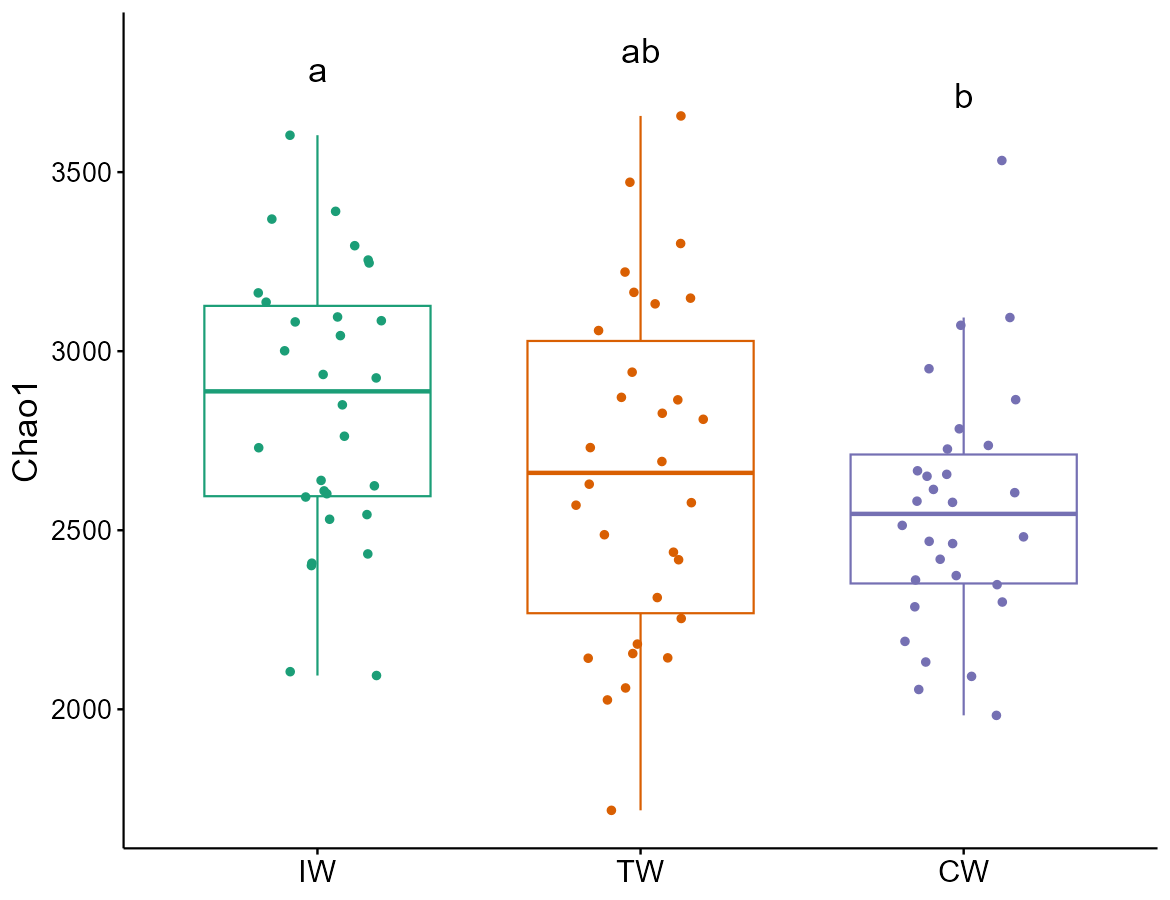
\includegraphics[width=600px]{Images/trans_alpha_group_letter} \end{center}

\begin{Shaded}
\begin{Highlighting}[]
\NormalTok{t1}\SpecialCharTok{$}\FunctionTok{cal\_diff}\NormalTok{(}\AttributeTok{method =} \StringTok{"wilcox"}\NormalTok{)}
\NormalTok{t1}\SpecialCharTok{$}\FunctionTok{plot\_alpha}\NormalTok{(}\AttributeTok{measure =} \StringTok{"Chao1"}\NormalTok{, }\AttributeTok{shape =} \StringTok{"Group"}\NormalTok{)}
\CommentTok{\# y\_start: starting height for the first label}
\CommentTok{\# y\_increase: increased height for each label}
\NormalTok{t1}\SpecialCharTok{$}\FunctionTok{plot\_alpha}\NormalTok{(}\AttributeTok{measure =} \StringTok{"Chao1"}\NormalTok{, }\AttributeTok{shape =} \StringTok{"Group"}\NormalTok{, }\AttributeTok{y\_start =} \FloatTok{0.1}\NormalTok{, }\AttributeTok{y\_increase =} \FloatTok{0.1}\NormalTok{)}
\end{Highlighting}
\end{Shaded}

\begin{center}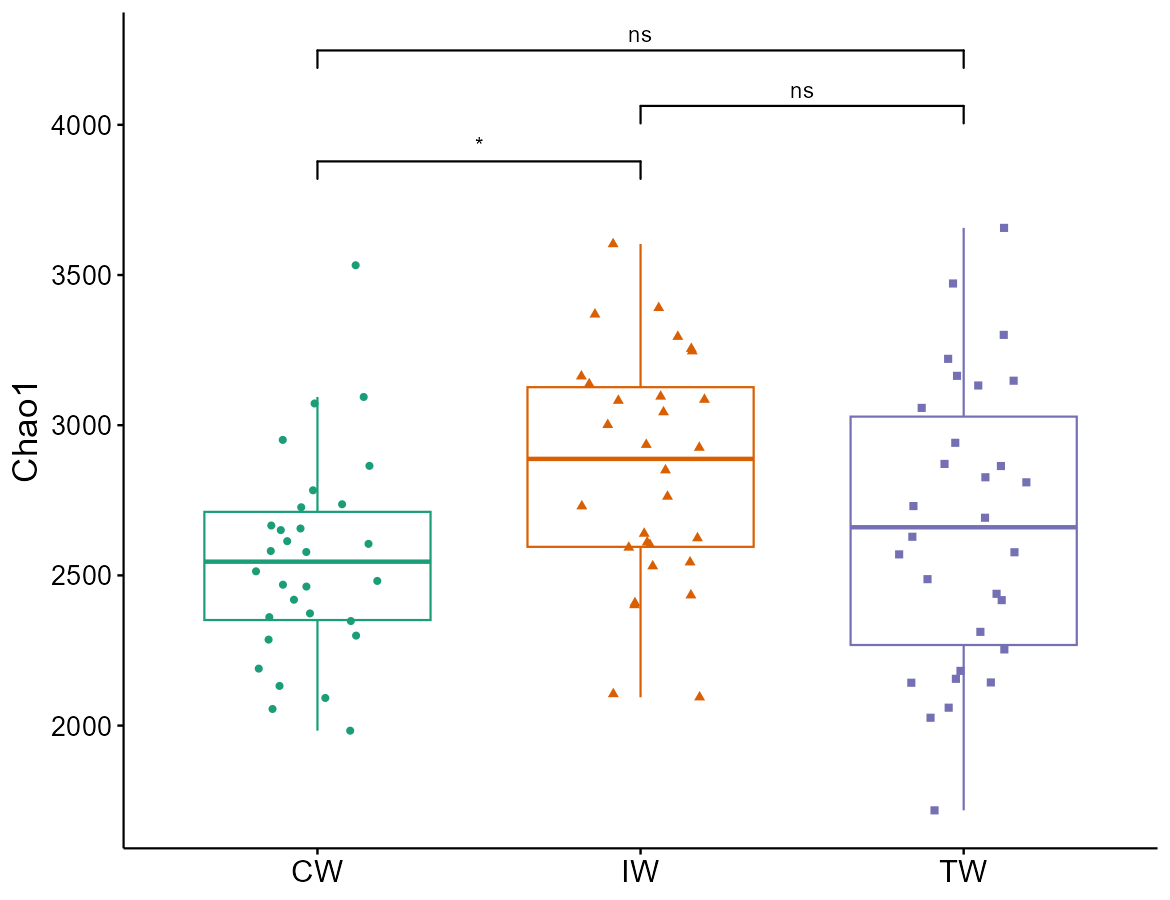
\includegraphics[width=600px]{Images/trans_alpha_group_wilcox} \end{center}

Let's try to remove the `ns' in the label by manipulating the object\$res\_diff.

\begin{Shaded}
\begin{Highlighting}[]
\NormalTok{t1}\SpecialCharTok{$}\NormalTok{res\_diff }\SpecialCharTok{\%\textless{}\textgreater{}\%}\NormalTok{ base}\SpecialCharTok{::}\FunctionTok{subset}\NormalTok{(Significance }\SpecialCharTok{!=} \StringTok{"ns"}\NormalTok{)}
\NormalTok{t1}\SpecialCharTok{$}\FunctionTok{plot\_alpha}\NormalTok{(}\AttributeTok{measure =} \StringTok{"Chao1"}\NormalTok{, }\AttributeTok{boxplot\_add =} \StringTok{"dotplot"}\NormalTok{, }\AttributeTok{xtext\_size =} \DecValTok{15}\NormalTok{)}
\end{Highlighting}
\end{Shaded}

\begin{center}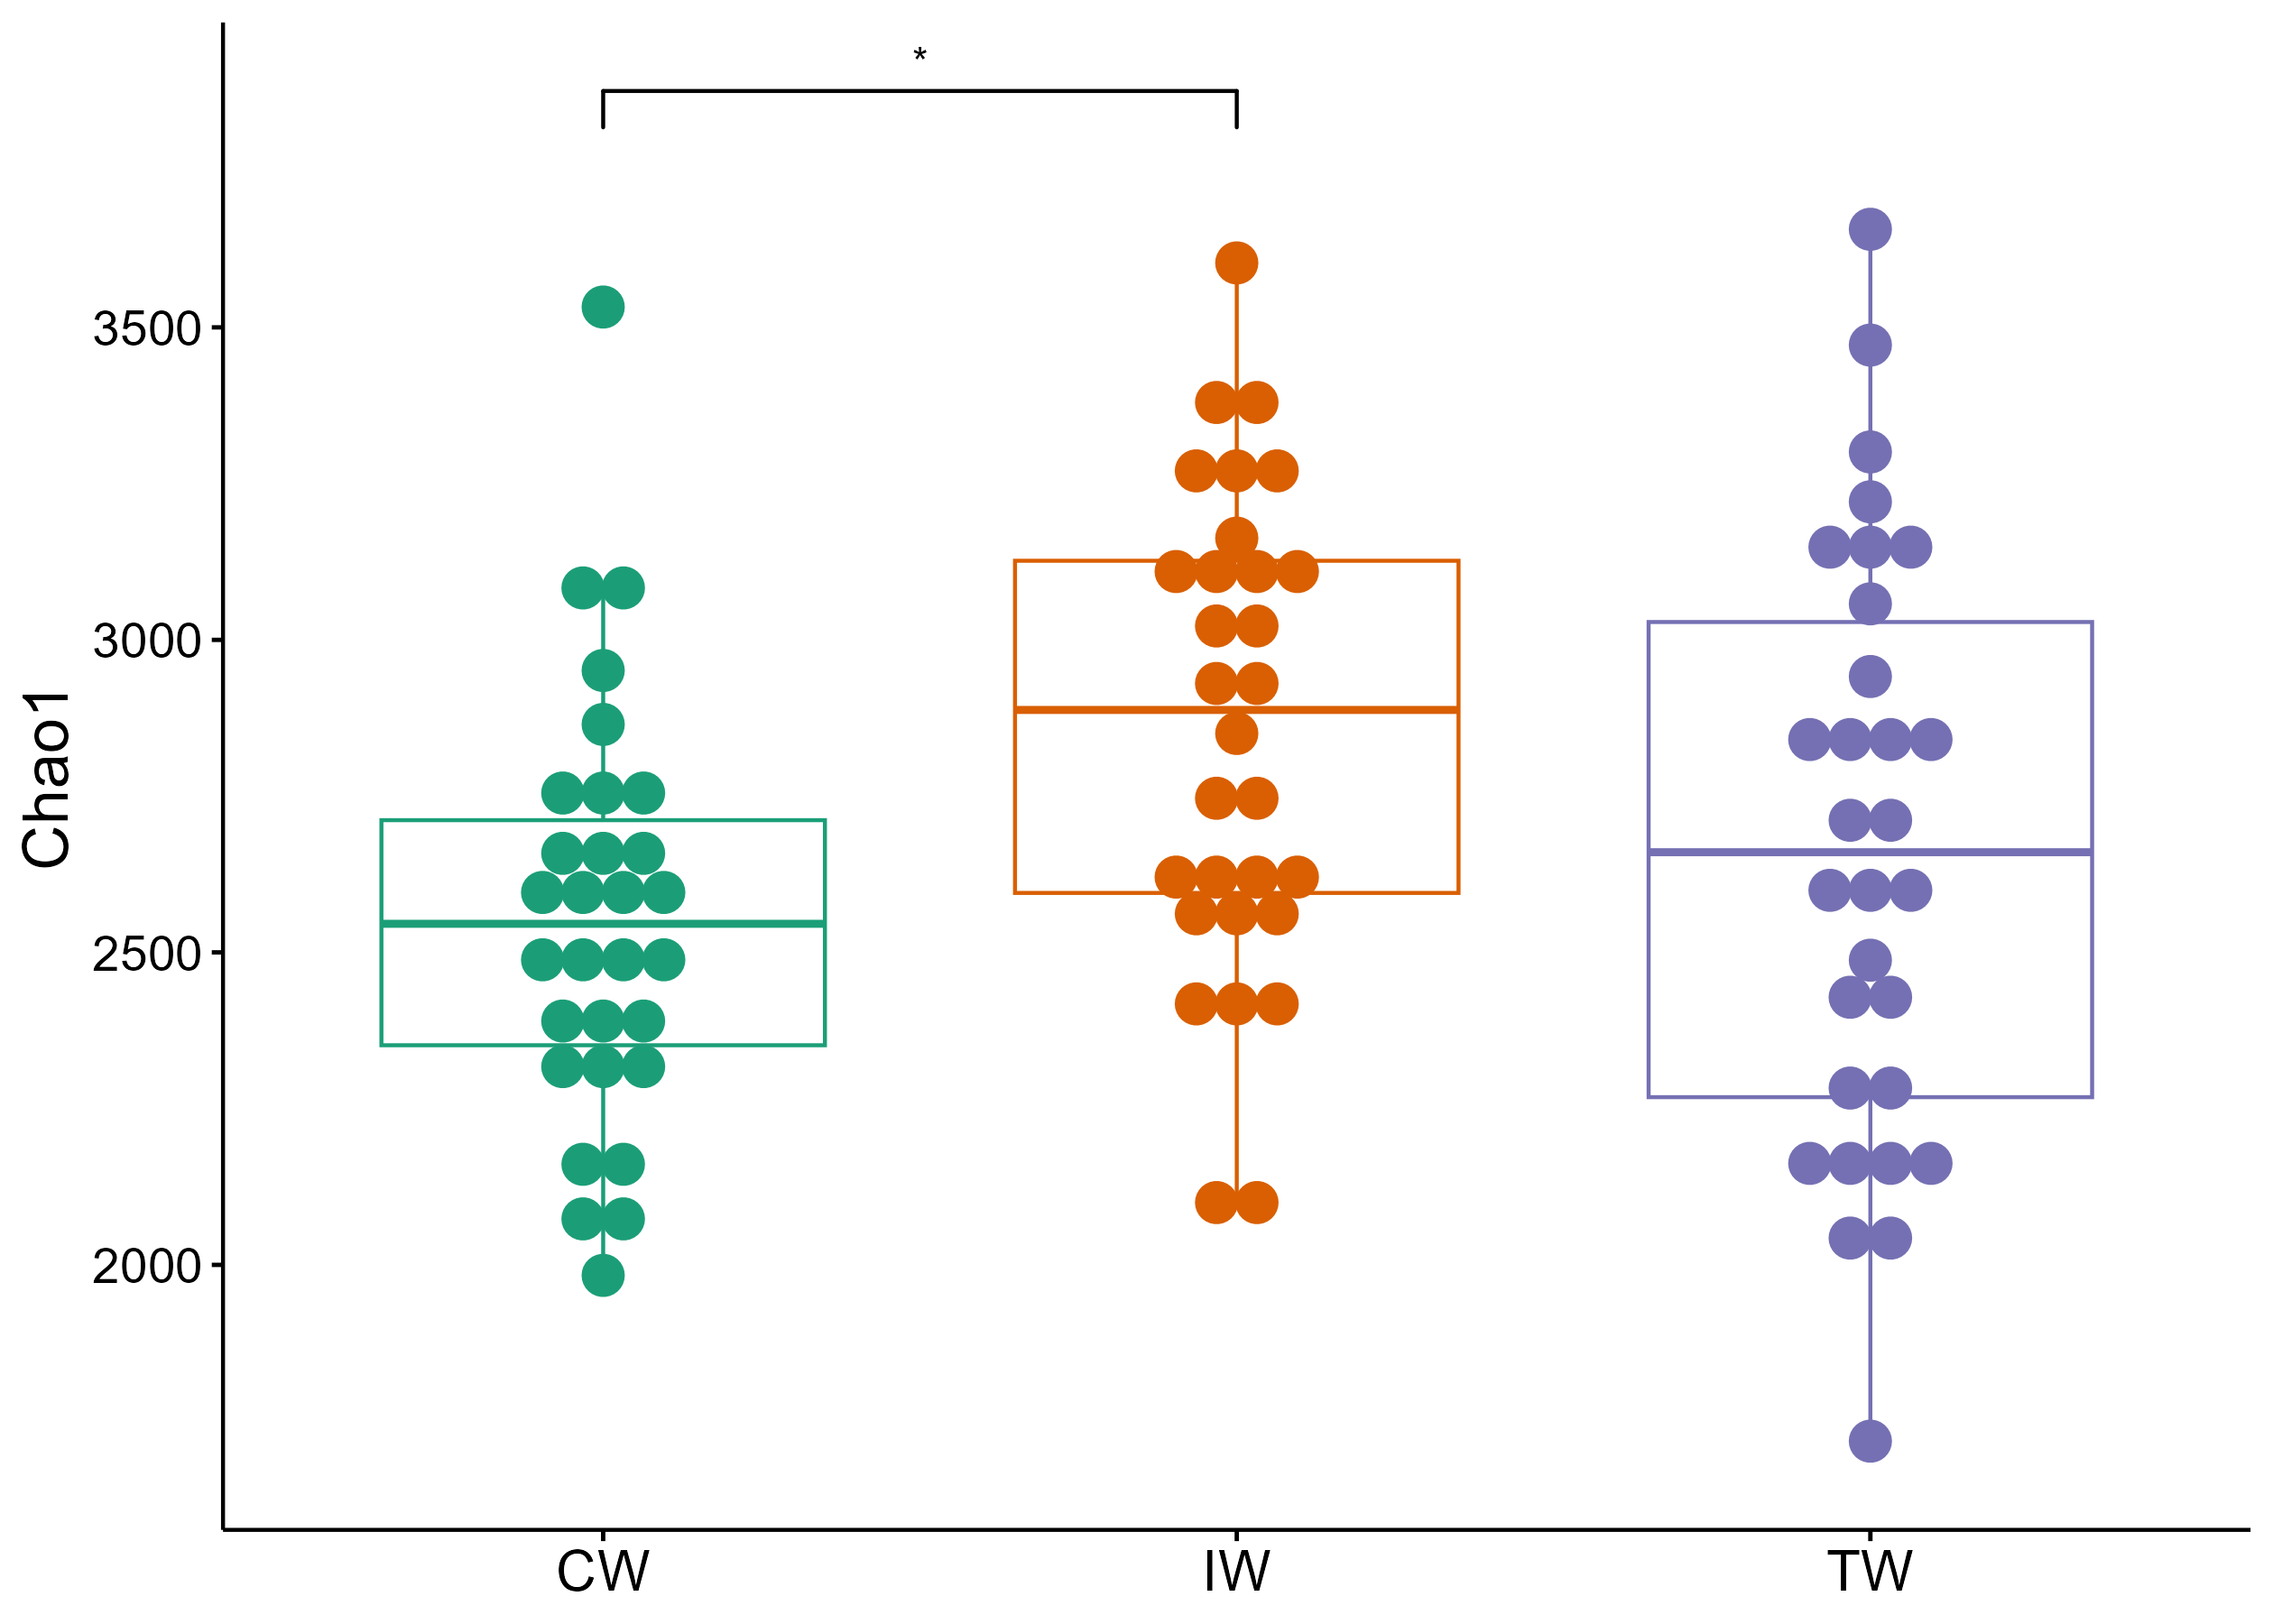
\includegraphics[width=600px]{Images/trans_alpha_wilcox_nons} \end{center}

The trans\_alpha class supports the differential test of groups within each group by using the by\_group parameter.

\begin{Shaded}
\begin{Highlighting}[]
\NormalTok{t1 }\OtherTok{\textless{}{-}}\NormalTok{ trans\_alpha}\SpecialCharTok{$}\FunctionTok{new}\NormalTok{(}\AttributeTok{dataset =}\NormalTok{ dataset, }\AttributeTok{group =} \StringTok{"Type"}\NormalTok{, }\AttributeTok{by\_group =} \StringTok{"Group"}\NormalTok{)}
\NormalTok{t1}\SpecialCharTok{$}\FunctionTok{cal\_diff}\NormalTok{(}\AttributeTok{method =} \StringTok{"wilcox"}\NormalTok{)}
\NormalTok{t1}\SpecialCharTok{$}\FunctionTok{plot\_alpha}\NormalTok{(}\AttributeTok{measure =} \StringTok{"Shannon"}\NormalTok{)}
\end{Highlighting}
\end{Shaded}

\begin{center}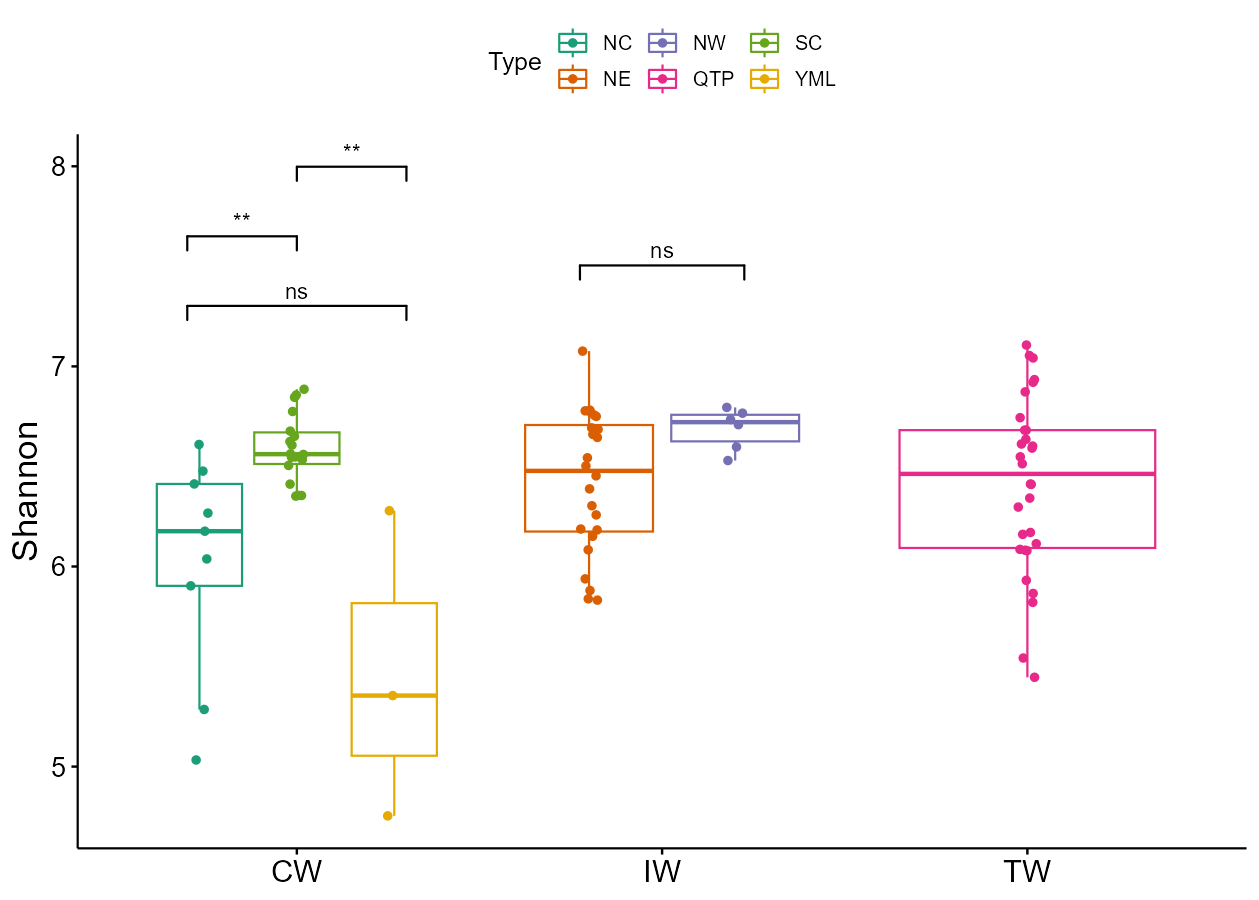
\includegraphics[width=600px]{Images/trans_alpha_wilcox_bygroup} \end{center}

Scheirer Ray Hare test is a nonparametric test that is suitable for a two-way factorial experiment.

\begin{Shaded}
\begin{Highlighting}[]
\CommentTok{\# require rcompanion package to be installed}
\NormalTok{t1}\SpecialCharTok{$}\FunctionTok{cal\_diff}\NormalTok{(}\AttributeTok{method =} \StringTok{"scheirerRayHare"}\NormalTok{, }\AttributeTok{formula =} \StringTok{"Group+Type"}\NormalTok{)}
\end{Highlighting}
\end{Shaded}

Linear mixed-effects model can be selected with the \texttt{method\ =\ "lme"}.
This model is implemented based on the \texttt{lmerTest} package.
For more parameters, please see \texttt{lmerTest::lmer} function.
Please use parameter passing when more parameters are needed.
For the formula usage, please follow this (\url{https://mspeekenbrink.github.io/sdam-r-companion/linear-mixed-effects-models.html}).
In the return table, conditional R2 is the total variance explained by fixed and random effects,
and marginal R2 is the variance explained by fixed effects.

\begin{Shaded}
\begin{Highlighting}[]
\ControlFlowTok{if}\NormalTok{(}\SpecialCharTok{!}\FunctionTok{require}\NormalTok{(}\StringTok{"lmerTest"}\NormalTok{)) }\FunctionTok{install.packages}\NormalTok{(}\StringTok{"lmerTest"}\NormalTok{)}
\NormalTok{t1 }\OtherTok{\textless{}{-}}\NormalTok{ trans\_alpha}\SpecialCharTok{$}\FunctionTok{new}\NormalTok{(}\AttributeTok{dataset =}\NormalTok{ dataset)}
\CommentTok{\# just using (1|Type) as an example to show the random effect}
\NormalTok{t1}\SpecialCharTok{$}\FunctionTok{cal\_diff}\NormalTok{(}\AttributeTok{method =} \StringTok{"lme"}\NormalTok{, }\AttributeTok{formula =} \StringTok{"Group + (1|Type)"}\NormalTok{)}
\FunctionTok{View}\NormalTok{(t1}\SpecialCharTok{$}\NormalTok{res\_diff)}
\CommentTok{\# return\_model = TRUE can return original models, i.e. object$res\_model}
\NormalTok{t1}\SpecialCharTok{$}\FunctionTok{cal\_diff}\NormalTok{(}\AttributeTok{method =} \StringTok{"lme"}\NormalTok{, }\AttributeTok{formula =} \StringTok{"Group + (1|Type)"}\NormalTok{, }\AttributeTok{return\_model =} \ConstantTok{TRUE}\NormalTok{)}
\end{Highlighting}
\end{Shaded}

Note that from v1.2.0, the parameter \texttt{use\_boxplot\ =\ FALSE} in \texttt{plot\_alpha} will invoke the data\_stat instead of data\_alpha for the Mean±SE (or SD) plot.
The line is optional to be added between points (Mean) for the case with a gradient.

\begin{Shaded}
\begin{Highlighting}[]
\NormalTok{t1 }\OtherTok{\textless{}{-}}\NormalTok{ trans\_alpha}\SpecialCharTok{$}\FunctionTok{new}\NormalTok{(}\AttributeTok{dataset =}\NormalTok{ dataset, }\AttributeTok{group =} \StringTok{"Group"}\NormalTok{)}
\NormalTok{t1}\SpecialCharTok{$}\FunctionTok{cal\_diff}\NormalTok{(}\AttributeTok{method =} \StringTok{"KW\_dunn"}\NormalTok{, }\AttributeTok{measure =} \StringTok{"PD"}\NormalTok{, }\AttributeTok{KW\_dunn\_letter =} \ConstantTok{TRUE}\NormalTok{)}
\NormalTok{t1}\SpecialCharTok{$}\FunctionTok{plot\_alpha}\NormalTok{(}\AttributeTok{measure =} \StringTok{"PD"}\NormalTok{)}
\NormalTok{t1}\SpecialCharTok{$}\FunctionTok{plot\_alpha}\NormalTok{(}\AttributeTok{use\_boxplot =} \ConstantTok{FALSE}\NormalTok{, }\AttributeTok{measure =} \StringTok{"PD"}\NormalTok{)}
\NormalTok{t1}\SpecialCharTok{$}\FunctionTok{plot\_alpha}\NormalTok{(}\AttributeTok{use\_boxplot =} \ConstantTok{FALSE}\NormalTok{, }\AttributeTok{measure =} \StringTok{"PD"}\NormalTok{, }\AttributeTok{y\_increase =} \SpecialCharTok{{-}}\FloatTok{0.2}\NormalTok{)}
\NormalTok{t1}\SpecialCharTok{$}\FunctionTok{plot\_alpha}\NormalTok{(}\AttributeTok{use\_boxplot =} \ConstantTok{FALSE}\NormalTok{, }\AttributeTok{measure =} \StringTok{"PD"}\NormalTok{, }\AttributeTok{y\_increase =} \SpecialCharTok{{-}}\FloatTok{0.2}\NormalTok{, }\AttributeTok{add\_line =} \ConstantTok{TRUE}\NormalTok{, }\AttributeTok{line\_type =} \DecValTok{2}\NormalTok{, }\AttributeTok{line\_alpha =} \FloatTok{0.5}\NormalTok{, }\AttributeTok{errorbar\_width =} \FloatTok{0.1}\NormalTok{)}
\NormalTok{t1}\SpecialCharTok{$}\FunctionTok{plot\_alpha}\NormalTok{(}\AttributeTok{use\_boxplot =} \ConstantTok{FALSE}\NormalTok{, }\AttributeTok{plot\_SE =} \ConstantTok{FALSE}\NormalTok{, }\AttributeTok{measure =} \StringTok{"PD"}\NormalTok{, }\AttributeTok{y\_increase =} \FloatTok{0.2}\NormalTok{, }\AttributeTok{add\_line =} \ConstantTok{TRUE}\NormalTok{, }\AttributeTok{line\_type =} \DecValTok{2}\NormalTok{, }\AttributeTok{line\_alpha =} \FloatTok{0.5}\NormalTok{, }\AttributeTok{errorbar\_width =} \FloatTok{0.1}\NormalTok{)}
\CommentTok{\# by\_group example}
\CommentTok{\# use example data in mecoturn package}
\FunctionTok{library}\NormalTok{(microeco)}
\FunctionTok{library}\NormalTok{(mecoturn)}
\FunctionTok{library}\NormalTok{(magrittr)}
\FunctionTok{data}\NormalTok{(wheat\_16S)}
\NormalTok{wheat\_16S}\SpecialCharTok{$}\NormalTok{sample\_table}\SpecialCharTok{$}\NormalTok{Type }\SpecialCharTok{\%\textless{}\textgreater{}\%} \FunctionTok{factor}\NormalTok{(., }\AttributeTok{levels =} \FunctionTok{unique}\NormalTok{(.))}
\NormalTok{t1 }\OtherTok{\textless{}{-}}\NormalTok{ trans\_alpha}\SpecialCharTok{$}\FunctionTok{new}\NormalTok{(}\AttributeTok{dataset =}\NormalTok{ wheat\_16S, }\AttributeTok{group =} \StringTok{"Region"}\NormalTok{, }\AttributeTok{by\_group =} \StringTok{"Type"}\NormalTok{)}
\NormalTok{t1}\SpecialCharTok{$}\FunctionTok{cal\_diff}\NormalTok{(}\AttributeTok{method =} \StringTok{"KW\_dunn"}\NormalTok{, }\AttributeTok{measure =} \StringTok{"Shannon"}\NormalTok{, }\AttributeTok{KW\_dunn\_letter =} \ConstantTok{TRUE}\NormalTok{)}
\FunctionTok{View}\NormalTok{(t1}\SpecialCharTok{$}\NormalTok{res\_diff)}
\NormalTok{t1}\SpecialCharTok{$}\FunctionTok{plot\_alpha}\NormalTok{(}\AttributeTok{use\_boxplot =} \ConstantTok{FALSE}\NormalTok{, }\AttributeTok{measure =} \StringTok{"Shannon"}\NormalTok{)}
\NormalTok{t1}\SpecialCharTok{$}\FunctionTok{plot\_alpha}\NormalTok{(}\AttributeTok{use\_boxplot =} \ConstantTok{FALSE}\NormalTok{, }\AttributeTok{measure =} \StringTok{"Shannon"}\NormalTok{, }\AttributeTok{add\_line =} \ConstantTok{TRUE}\NormalTok{, }\AttributeTok{line\_type =} \DecValTok{2}\NormalTok{)}
\NormalTok{t1}\SpecialCharTok{$}\FunctionTok{plot\_alpha}\NormalTok{(}\AttributeTok{use\_boxplot =} \ConstantTok{FALSE}\NormalTok{, }\AttributeTok{plot\_SE =} \ConstantTok{FALSE}\NormalTok{, }\AttributeTok{measure =} \StringTok{"Shannon"}\NormalTok{, }\AttributeTok{add\_line =} \ConstantTok{TRUE}\NormalTok{, }\AttributeTok{line\_type =} \DecValTok{2}\NormalTok{)}
\end{Highlighting}
\end{Shaded}

\hypertarget{key-points-3}{%
\subsection{Key points}\label{key-points-3}}

\begin{itemize}
\tightlist
\item
  trans\_alpha\$new: creating \texttt{trans\_alpha} object can invoke \texttt{alpha\_diversity} in microtable for transformation
\item
  cal\_diff: \texttt{formula} parameter applies to multi-factor analysis of variance.
\item
  cal\_diff: From v1.2.0, \texttt{anova\_post\_test} can be used to change default post test method of anova.
\item
  plot\_alpha: the significance label comes from the results in \texttt{object\$res\_diff}
\end{itemize}

\hypertarget{trans_beta-class}{%
\section{trans\_beta class}\label{trans_beta-class}}

 The trans\_beta class is specifically designed for the beta diversity analysis, i.e.~the dissimilarities among samples.
Beta diversity can be defined at different forms\citep{Tuomisto_diversity_2010} and can be explored with different ways\citep{Anderson_Navigating_2011}.
We encapsulate some commonly-used approaches in microbial ecology\citep{Ramette_Multivariate_2007}.
Note that the part of beta diversity related with environmental factors are placed into the trans\_env class.
The distance matrix in beta\_diversity list of microtable object will be invoked for transformation and ploting using trans\_beta class when needed.
The analysis referred to the beta diversity in this class mainly include ordination, group distance, clustering and manova.

\hypertarget{example-3}{%
\subsection{Example}\label{example-3}}

We first show the ordination using PCoA (principal coordinates analysis).

\begin{Shaded}
\begin{Highlighting}[]
\CommentTok{\# create an trans\_beta object}
\CommentTok{\# measure parameter must be one of names(dataset$beta\_diversity)}
\NormalTok{t1 }\OtherTok{\textless{}{-}}\NormalTok{ trans\_beta}\SpecialCharTok{$}\FunctionTok{new}\NormalTok{(}\AttributeTok{dataset =}\NormalTok{ dataset, }\AttributeTok{group =} \StringTok{"Group"}\NormalTok{, }\AttributeTok{measure =} \StringTok{"bray"}\NormalTok{)}
\end{Highlighting}
\end{Shaded}

\begin{Shaded}
\begin{Highlighting}[]
\CommentTok{\# PCoA, PCA and NMDS are available}
\NormalTok{t1}\SpecialCharTok{$}\FunctionTok{cal\_ordination}\NormalTok{(}\AttributeTok{ordination =} \StringTok{"PCoA"}\NormalTok{)}
\CommentTok{\# t1$res\_ordination is the ordination result list}
\FunctionTok{class}\NormalTok{(t1}\SpecialCharTok{$}\NormalTok{res\_ordination)}
\CommentTok{\# plot the PCoA result with confidence ellipse}
\NormalTok{t1}\SpecialCharTok{$}\FunctionTok{plot\_ordination}\NormalTok{(}\AttributeTok{plot\_color =} \StringTok{"Group"}\NormalTok{, }\AttributeTok{plot\_shape =} \StringTok{"Group"}\NormalTok{, }\AttributeTok{plot\_type =} \FunctionTok{c}\NormalTok{(}\StringTok{"point"}\NormalTok{, }\StringTok{"ellipse"}\NormalTok{))}
\end{Highlighting}
\end{Shaded}

\begin{center}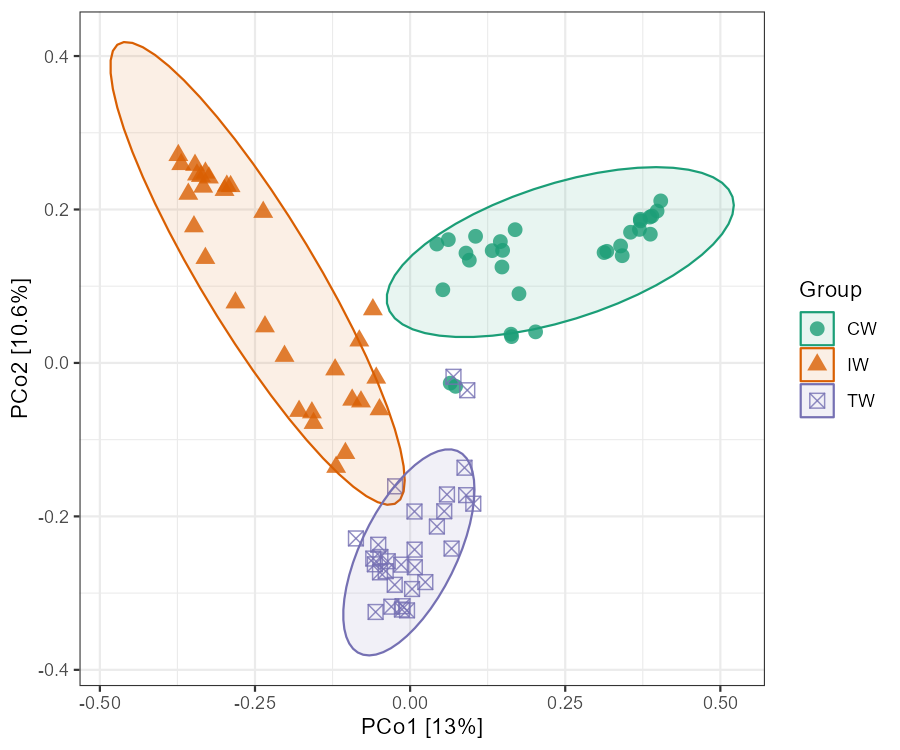
\includegraphics[width=650px]{Images/trans_beta_ordination} \end{center}

More examples on different options.

\begin{Shaded}
\begin{Highlighting}[]
\NormalTok{t1}\SpecialCharTok{$}\FunctionTok{plot\_ordination}\NormalTok{(}\AttributeTok{plot\_color =} \StringTok{"Type"}\NormalTok{, }\AttributeTok{plot\_type =} \StringTok{"point"}\NormalTok{)}
\NormalTok{t1}\SpecialCharTok{$}\FunctionTok{plot\_ordination}\NormalTok{(}\AttributeTok{plot\_color =} \StringTok{"Group"}\NormalTok{, }\AttributeTok{point\_size =} \DecValTok{5}\NormalTok{, }\AttributeTok{point\_alpha =}\NormalTok{ .}\DecValTok{2}\NormalTok{, }\AttributeTok{plot\_type =} \FunctionTok{c}\NormalTok{(}\StringTok{"point"}\NormalTok{, }\StringTok{"ellipse"}\NormalTok{), }\AttributeTok{ellipse\_chull\_fill =} \ConstantTok{FALSE}\NormalTok{)}
\NormalTok{t1}\SpecialCharTok{$}\FunctionTok{plot\_ordination}\NormalTok{(}\AttributeTok{plot\_color =} \StringTok{"Group"}\NormalTok{, }\AttributeTok{plot\_shape =} \StringTok{"Group"}\NormalTok{, }\AttributeTok{plot\_type =} \FunctionTok{c}\NormalTok{(}\StringTok{"point"}\NormalTok{, }\StringTok{"centroid"}\NormalTok{))}
\NormalTok{t1}\SpecialCharTok{$}\FunctionTok{plot\_ordination}\NormalTok{(}\AttributeTok{plot\_color =} \StringTok{"Group"}\NormalTok{, }\AttributeTok{plot\_shape =} \StringTok{"Group"}\NormalTok{, }\AttributeTok{plot\_type =} \FunctionTok{c}\NormalTok{(}\StringTok{"point"}\NormalTok{, }\StringTok{"ellipse"}\NormalTok{, }\StringTok{"centroid"}\NormalTok{))}
\NormalTok{t1}\SpecialCharTok{$}\FunctionTok{plot\_ordination}\NormalTok{(}\AttributeTok{plot\_color =} \StringTok{"Group"}\NormalTok{, }\AttributeTok{plot\_shape =} \StringTok{"Group"}\NormalTok{, }\AttributeTok{plot\_type =} \FunctionTok{c}\NormalTok{(}\StringTok{"point"}\NormalTok{, }\StringTok{"chull"}\NormalTok{))}
\NormalTok{t1}\SpecialCharTok{$}\FunctionTok{plot\_ordination}\NormalTok{(}\AttributeTok{plot\_color =} \StringTok{"Group"}\NormalTok{, }\AttributeTok{plot\_shape =} \StringTok{"Group"}\NormalTok{, }\AttributeTok{plot\_type =} \FunctionTok{c}\NormalTok{(}\StringTok{"point"}\NormalTok{, }\StringTok{"chull"}\NormalTok{, }\StringTok{"centroid"}\NormalTok{))}
\NormalTok{t1}\SpecialCharTok{$}\FunctionTok{plot\_ordination}\NormalTok{(}\AttributeTok{plot\_color =} \StringTok{"Group"}\NormalTok{, }\AttributeTok{plot\_shape =} \StringTok{"Group"}\NormalTok{, }\AttributeTok{plot\_type =} \FunctionTok{c}\NormalTok{(}\StringTok{"chull"}\NormalTok{, }\StringTok{"centroid"}\NormalTok{))}
\NormalTok{t1}\SpecialCharTok{$}\FunctionTok{plot\_ordination}\NormalTok{(}\AttributeTok{plot\_color =} \StringTok{"Group"}\NormalTok{, }\AttributeTok{plot\_shape =} \StringTok{"Group"}\NormalTok{, }\AttributeTok{plot\_type =} \FunctionTok{c}\NormalTok{(}\StringTok{"point"}\NormalTok{, }\StringTok{"chull"}\NormalTok{, }\StringTok{"centroid"}\NormalTok{), }\AttributeTok{add\_sample\_label =} \StringTok{"SampleID"}\NormalTok{)}
\NormalTok{t1}\SpecialCharTok{$}\FunctionTok{plot\_ordination}\NormalTok{(}\AttributeTok{plot\_color =} \StringTok{"Group"}\NormalTok{, }\AttributeTok{plot\_shape =} \StringTok{"Group"}\NormalTok{, }\AttributeTok{plot\_type =} \StringTok{"centroid"}\NormalTok{)}
\NormalTok{t1}\SpecialCharTok{$}\FunctionTok{plot\_ordination}\NormalTok{(}\AttributeTok{plot\_color =} \StringTok{"Group"}\NormalTok{, }\AttributeTok{plot\_shape =} \StringTok{"Group"}\NormalTok{, }\AttributeTok{plot\_type =} \StringTok{"centroid"}\NormalTok{, }\AttributeTok{centroid\_segment\_alpha =} \FloatTok{0.9}\NormalTok{, }\AttributeTok{centroid\_segment\_size =} \DecValTok{1}\NormalTok{, }\AttributeTok{centroid\_segment\_linetype =} \DecValTok{1}\NormalTok{)}
\NormalTok{t1}\SpecialCharTok{$}\FunctionTok{plot\_ordination}\NormalTok{(}\AttributeTok{plot\_type =} \FunctionTok{c}\NormalTok{(}\StringTok{"point"}\NormalTok{, }\StringTok{"centroid"}\NormalTok{), }\AttributeTok{plot\_color =} \StringTok{"Type"}\NormalTok{, }\AttributeTok{centroid\_segment\_linetype =} \DecValTok{1}\NormalTok{)}
\NormalTok{t1}\SpecialCharTok{$}\FunctionTok{plot\_ordination}\NormalTok{(}\AttributeTok{plot\_color =} \StringTok{"Saline"}\NormalTok{, }\AttributeTok{point\_size =} \DecValTok{5}\NormalTok{, }\AttributeTok{point\_alpha =}\NormalTok{ .}\DecValTok{2}\NormalTok{, }\AttributeTok{plot\_type =} \FunctionTok{c}\NormalTok{(}\StringTok{"point"}\NormalTok{, }\StringTok{"chull"}\NormalTok{), }\AttributeTok{ellipse\_chull\_fill =} \ConstantTok{FALSE}\NormalTok{, }\AttributeTok{ellipse\_chull\_alpha =} \FloatTok{0.1}\NormalTok{)}
\NormalTok{t1}\SpecialCharTok{$}\FunctionTok{plot\_ordination}\NormalTok{(}\AttributeTok{plot\_color =} \StringTok{"Group"}\NormalTok{) }\SpecialCharTok{+} \FunctionTok{theme}\NormalTok{(}\AttributeTok{panel.grid =} \FunctionTok{element\_blank}\NormalTok{()) }\SpecialCharTok{+} \FunctionTok{geom\_vline}\NormalTok{(}\AttributeTok{xintercept =} \DecValTok{0}\NormalTok{, }\AttributeTok{linetype =} \DecValTok{2}\NormalTok{) }\SpecialCharTok{+} \FunctionTok{geom\_hline}\NormalTok{(}\AttributeTok{yintercept =} \DecValTok{0}\NormalTok{, }\AttributeTok{linetype =} \DecValTok{2}\NormalTok{)}
\end{Highlighting}
\end{Shaded}

Then we plot and compare the group distances.

\begin{Shaded}
\begin{Highlighting}[]
\CommentTok{\# calculate and plot sample distances within groups}
\NormalTok{t1}\SpecialCharTok{$}\FunctionTok{cal\_group\_distance}\NormalTok{(}\AttributeTok{within\_group =} \ConstantTok{TRUE}\NormalTok{)}
\CommentTok{\# return t1$res\_group\_distance}
\CommentTok{\# perform Wilcoxon Rank Sum and Signed Rank Tests}
\NormalTok{t1}\SpecialCharTok{$}\FunctionTok{cal\_group\_distance\_diff}\NormalTok{(}\AttributeTok{method =} \StringTok{"wilcox"}\NormalTok{)}
\CommentTok{\# plot\_group\_order parameter can be used to adjust orders in x axis}
\NormalTok{t1}\SpecialCharTok{$}\FunctionTok{plot\_group\_distance}\NormalTok{(}\AttributeTok{boxplot\_add =} \StringTok{"mean"}\NormalTok{)}
\end{Highlighting}
\end{Shaded}

\begin{center}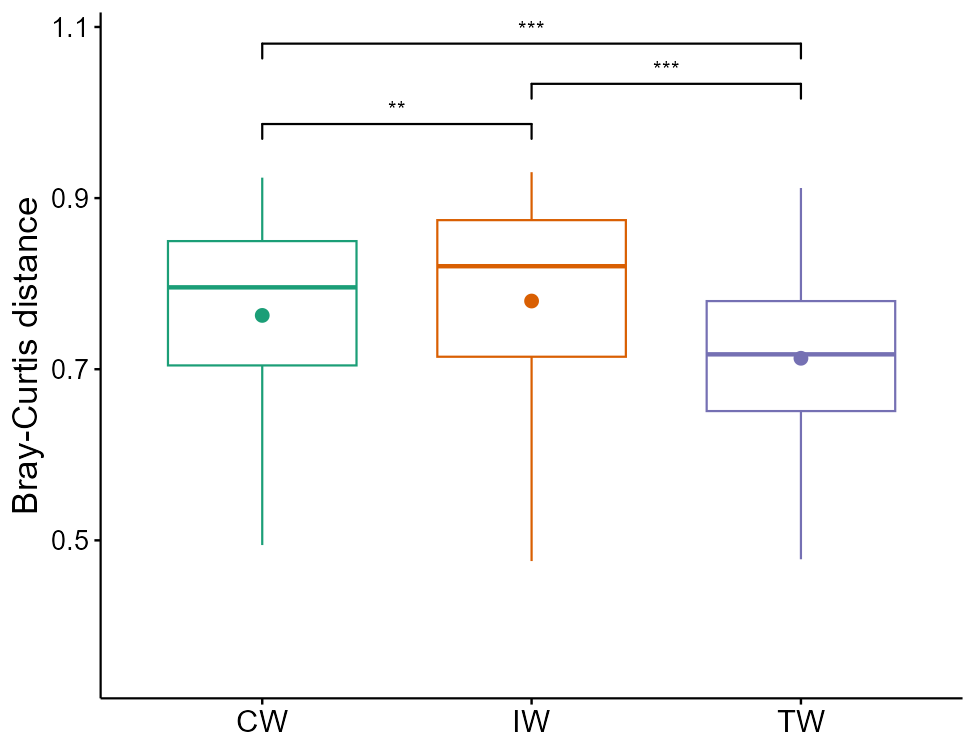
\includegraphics[width=500px]{Images/trans_beta_group_distance_within} \end{center}

\begin{Shaded}
\begin{Highlighting}[]
\CommentTok{\# calculate and plot sample distances between groups}
\NormalTok{t1}\SpecialCharTok{$}\FunctionTok{cal\_group\_distance}\NormalTok{(}\AttributeTok{within\_group =} \ConstantTok{FALSE}\NormalTok{)}
\NormalTok{t1}\SpecialCharTok{$}\FunctionTok{cal\_group\_distance\_diff}\NormalTok{(}\AttributeTok{method =} \StringTok{"wilcox"}\NormalTok{)}
\NormalTok{t1}\SpecialCharTok{$}\FunctionTok{plot\_group\_distance}\NormalTok{(}\AttributeTok{boxplot\_add =} \StringTok{"mean"}\NormalTok{)}
\end{Highlighting}
\end{Shaded}

\begin{center}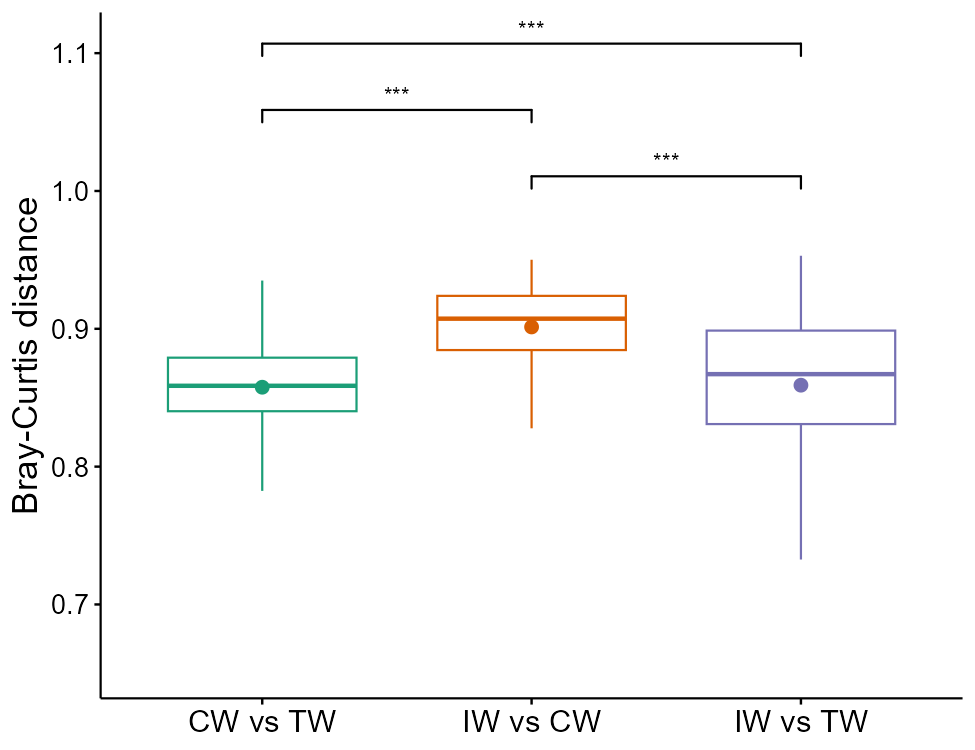
\includegraphics[width=500px]{Images/trans_beta_group_distance_between} \end{center}

Clustering plot is also a frequently used method.

\begin{Shaded}
\begin{Highlighting}[]
\CommentTok{\# extract a part of data}
\NormalTok{d1 }\OtherTok{\textless{}{-}} \FunctionTok{clone}\NormalTok{(dataset)}
\NormalTok{d1}\SpecialCharTok{$}\NormalTok{sample\_table }\SpecialCharTok{\%\textless{}\textgreater{}\%} \FunctionTok{subset}\NormalTok{(Group }\SpecialCharTok{\%in\%} \FunctionTok{c}\NormalTok{(}\StringTok{"CW"}\NormalTok{, }\StringTok{"TW"}\NormalTok{))}
\NormalTok{d1}\SpecialCharTok{$}\FunctionTok{tidy\_dataset}\NormalTok{()}
\NormalTok{t1 }\OtherTok{\textless{}{-}}\NormalTok{ trans\_beta}\SpecialCharTok{$}\FunctionTok{new}\NormalTok{(}\AttributeTok{dataset =}\NormalTok{ d1, }\AttributeTok{group =} \StringTok{"Group"}\NormalTok{)}
\CommentTok{\# use replace\_name to set the label name, group parameter used to set the color}
\NormalTok{t1}\SpecialCharTok{$}\FunctionTok{plot\_clustering}\NormalTok{(}\AttributeTok{group =} \StringTok{"Type"}\NormalTok{, }\AttributeTok{replace\_name =} \FunctionTok{c}\NormalTok{(}\StringTok{"Type"}\NormalTok{))}
\end{Highlighting}
\end{Shaded}

\begin{center}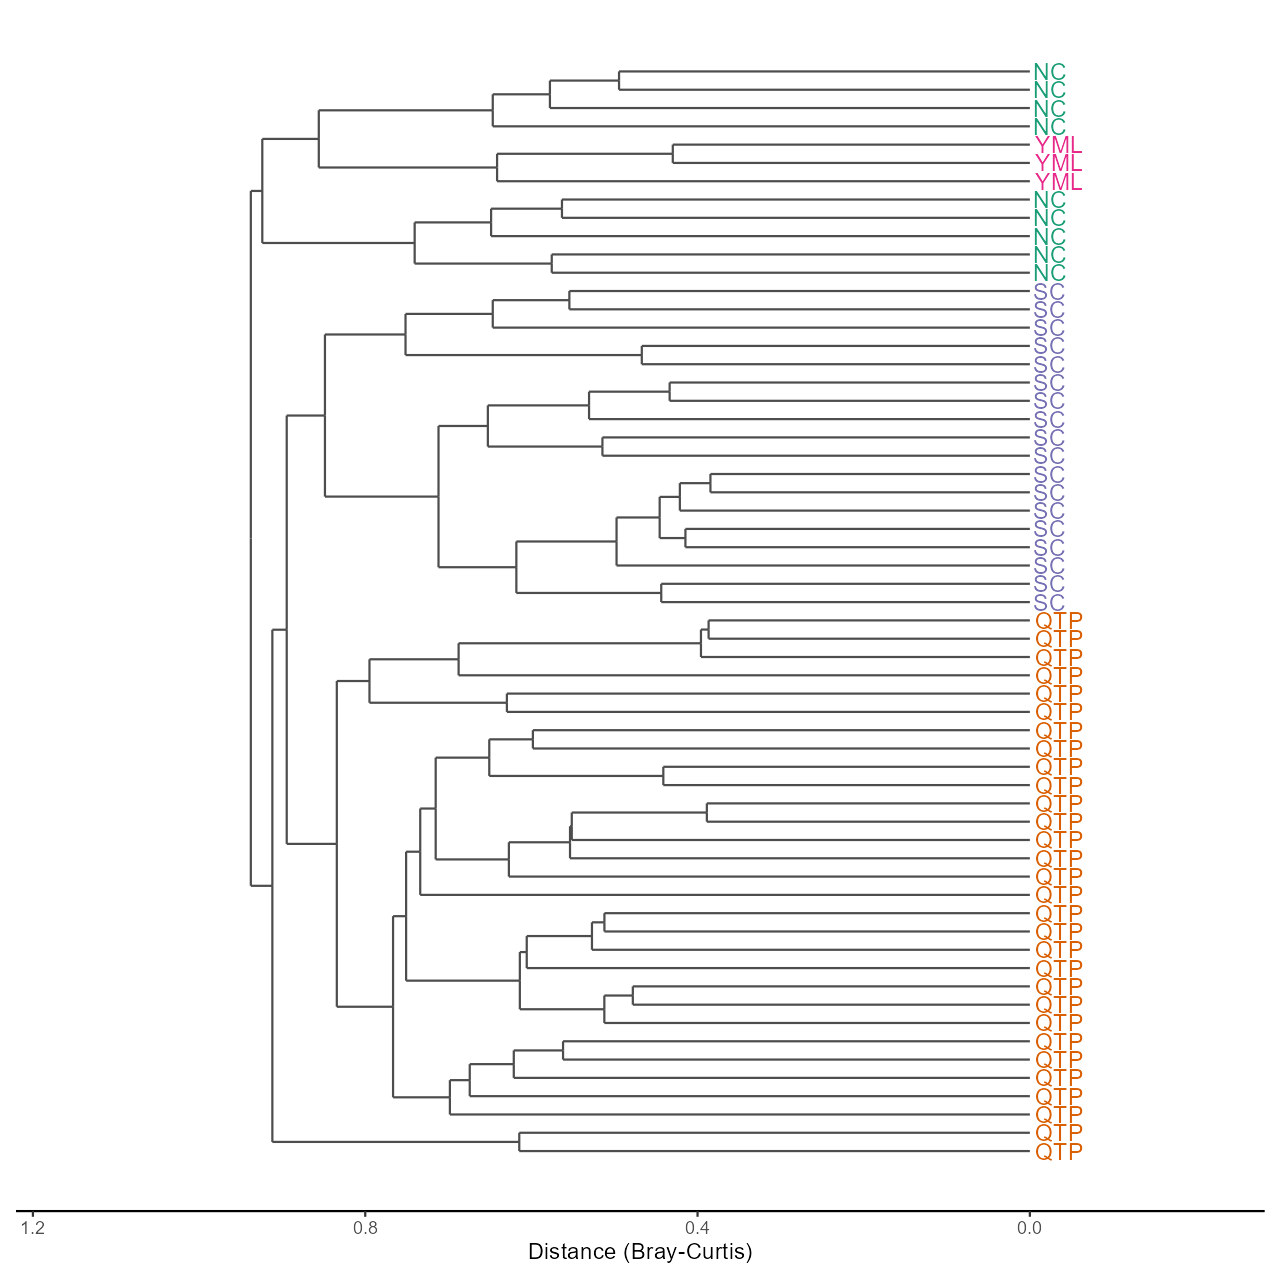
\includegraphics[width=550px]{Images/trans_beta_clustering} \end{center}

PerMANOVA\citep{Anderson_Austral_2001} can be applied to the differential test of distances among groups via the \texttt{cal\_manova} function developed
based on the \texttt{adonis2} function of vegan package.

\begin{Shaded}
\begin{Highlighting}[]
\CommentTok{\# manova for all groups when manova\_all = TRUE}
\NormalTok{t1}\SpecialCharTok{$}\FunctionTok{cal\_manova}\NormalTok{(}\AttributeTok{manova\_all =} \ConstantTok{TRUE}\NormalTok{)}
\NormalTok{t1}\SpecialCharTok{$}\NormalTok{res\_manova}
\end{Highlighting}
\end{Shaded}

\begin{verbatim}
## The result is stored in object$res_manova ...
\end{verbatim}

\begin{longtable}[]{@{}
  >{\centering\arraybackslash}p{(\columnwidth - 10\tabcolsep) * \real{0.2083}}
  >{\centering\arraybackslash}p{(\columnwidth - 10\tabcolsep) * \real{0.0694}}
  >{\centering\arraybackslash}p{(\columnwidth - 10\tabcolsep) * \real{0.1528}}
  >{\centering\arraybackslash}p{(\columnwidth - 10\tabcolsep) * \real{0.1250}}
  >{\centering\arraybackslash}p{(\columnwidth - 10\tabcolsep) * \real{0.1111}}
  >{\centering\arraybackslash}p{(\columnwidth - 10\tabcolsep) * \real{0.1250}}@{}}
\caption{Permutation test for adonis under reduced model}\tabularnewline
\toprule()
\begin{minipage}[b]{\linewidth}\centering
~
\end{minipage} & \begin{minipage}[b]{\linewidth}\centering
Df
\end{minipage} & \begin{minipage}[b]{\linewidth}\centering
SumOfSqs
\end{minipage} & \begin{minipage}[b]{\linewidth}\centering
R2
\end{minipage} & \begin{minipage}[b]{\linewidth}\centering
F
\end{minipage} & \begin{minipage}[b]{\linewidth}\centering
Pr(\textgreater F)
\end{minipage} \\
\midrule()
\endfirsthead
\toprule()
\begin{minipage}[b]{\linewidth}\centering
~
\end{minipage} & \begin{minipage}[b]{\linewidth}\centering
Df
\end{minipage} & \begin{minipage}[b]{\linewidth}\centering
SumOfSqs
\end{minipage} & \begin{minipage}[b]{\linewidth}\centering
R2
\end{minipage} & \begin{minipage}[b]{\linewidth}\centering
F
\end{minipage} & \begin{minipage}[b]{\linewidth}\centering
Pr(\textgreater F)
\end{minipage} \\
\midrule()
\endhead
\textbf{Group} & 2 & 6.121 & 0.1955 & 10.57 & 0.001 \\
\textbf{Residual} & 87 & 25.18 & 0.8045 & NA & NA \\
\textbf{Total} & 89 & 31.3 & 1 & NA & NA \\
\bottomrule()
\end{longtable}

The parameter \texttt{manova\_all\ =\ FALSE} can make the test switch to paired group comparison.

\begin{Shaded}
\begin{Highlighting}[]
\CommentTok{\# manova for each paired groups}
\NormalTok{t1}\SpecialCharTok{$}\FunctionTok{cal\_manova}\NormalTok{(}\AttributeTok{manova\_all =} \ConstantTok{FALSE}\NormalTok{)}
\NormalTok{t1}\SpecialCharTok{$}\NormalTok{res\_manova}
\end{Highlighting}
\end{Shaded}

\begin{verbatim}
## The result is stored in object$res_manova ...
\end{verbatim}

\begin{longtable}[]{@{}
  >{\centering\arraybackslash}p{(\columnwidth - 12\tabcolsep) * \real{0.1447}}
  >{\centering\arraybackslash}p{(\columnwidth - 12\tabcolsep) * \real{0.1316}}
  >{\centering\arraybackslash}p{(\columnwidth - 12\tabcolsep) * \real{0.1053}}
  >{\centering\arraybackslash}p{(\columnwidth - 12\tabcolsep) * \real{0.1184}}
  >{\centering\arraybackslash}p{(\columnwidth - 12\tabcolsep) * \real{0.1316}}
  >{\centering\arraybackslash}p{(\columnwidth - 12\tabcolsep) * \real{0.1711}}
  >{\centering\arraybackslash}p{(\columnwidth - 12\tabcolsep) * \real{0.1974}}@{}}
\toprule()
\begin{minipage}[b]{\linewidth}\centering
Groups
\end{minipage} & \begin{minipage}[b]{\linewidth}\centering
measure
\end{minipage} & \begin{minipage}[b]{\linewidth}\centering
F
\end{minipage} & \begin{minipage}[b]{\linewidth}\centering
R2
\end{minipage} & \begin{minipage}[b]{\linewidth}\centering
p.value
\end{minipage} & \begin{minipage}[b]{\linewidth}\centering
p.adjusted
\end{minipage} & \begin{minipage}[b]{\linewidth}\centering
Significance
\end{minipage} \\
\midrule()
\endhead
IW vs CW & bray & 11.01 & 0.1595 & 0.001 & 0.001 & *** \\
IW vs TW & bray & 9.992 & 0.147 & 0.001 & 0.001 & *** \\
CW vs TW & bray & 10.69 & 0.1556 & 0.001 & 0.001 & *** \\
\bottomrule()
\end{longtable}

The parameter \texttt{manova\_set} has higher priority than \texttt{manova\_all}. If \texttt{manova\_set} is provided, manova\_all parameter will be disabled.

\begin{Shaded}
\begin{Highlighting}[]
\CommentTok{\# manova for specified group set: such as "Group + Type"}
\NormalTok{t1}\SpecialCharTok{$}\FunctionTok{cal\_manova}\NormalTok{(}\AttributeTok{manova\_set =} \StringTok{"Group + Type"}\NormalTok{)}
\NormalTok{t1}\SpecialCharTok{$}\NormalTok{res\_manova}
\end{Highlighting}
\end{Shaded}

\begin{verbatim}
## The result is stored in object$res_manova ...
\end{verbatim}

\begin{longtable}[]{@{}
  >{\centering\arraybackslash}p{(\columnwidth - 10\tabcolsep) * \real{0.2083}}
  >{\centering\arraybackslash}p{(\columnwidth - 10\tabcolsep) * \real{0.0694}}
  >{\centering\arraybackslash}p{(\columnwidth - 10\tabcolsep) * \real{0.1528}}
  >{\centering\arraybackslash}p{(\columnwidth - 10\tabcolsep) * \real{0.1250}}
  >{\centering\arraybackslash}p{(\columnwidth - 10\tabcolsep) * \real{0.1111}}
  >{\centering\arraybackslash}p{(\columnwidth - 10\tabcolsep) * \real{0.1250}}@{}}
\caption{Permutation test for adonis under reduced model}\tabularnewline
\toprule()
\begin{minipage}[b]{\linewidth}\centering
~
\end{minipage} & \begin{minipage}[b]{\linewidth}\centering
Df
\end{minipage} & \begin{minipage}[b]{\linewidth}\centering
SumOfSqs
\end{minipage} & \begin{minipage}[b]{\linewidth}\centering
R2
\end{minipage} & \begin{minipage}[b]{\linewidth}\centering
F
\end{minipage} & \begin{minipage}[b]{\linewidth}\centering
Pr(\textgreater F)
\end{minipage} \\
\midrule()
\endfirsthead
\toprule()
\begin{minipage}[b]{\linewidth}\centering
~
\end{minipage} & \begin{minipage}[b]{\linewidth}\centering
Df
\end{minipage} & \begin{minipage}[b]{\linewidth}\centering
SumOfSqs
\end{minipage} & \begin{minipage}[b]{\linewidth}\centering
R2
\end{minipage} & \begin{minipage}[b]{\linewidth}\centering
F
\end{minipage} & \begin{minipage}[b]{\linewidth}\centering
Pr(\textgreater F)
\end{minipage} \\
\midrule()
\endhead
\textbf{Group} & 2 & 6.121 & 0.1955 & 12.01 & 0.001 \\
\textbf{Type} & 3 & 3.783 & 0.1208 & 4.949 & 0.001 \\
\textbf{Residual} & 84 & 21.4 & 0.6836 & NA & NA \\
\textbf{Total} & 89 & 31.3 & 1 & NA & NA \\
\bottomrule()
\end{longtable}

From v1.0.0, ANOSIM method is also available.

\begin{Shaded}
\begin{Highlighting}[]
\CommentTok{\# the group parameter is not necessary when it is provided in creating the object}
\NormalTok{t1}\SpecialCharTok{$}\FunctionTok{cal\_anosim}\NormalTok{(}\AttributeTok{group =} \StringTok{"Group"}\NormalTok{)}
\NormalTok{t1}\SpecialCharTok{$}\NormalTok{res\_anosim}
\NormalTok{t1}\SpecialCharTok{$}\FunctionTok{cal\_anosim}\NormalTok{(}\AttributeTok{group =} \StringTok{"Group"}\NormalTok{, }\AttributeTok{paired =} \ConstantTok{TRUE}\NormalTok{)}
\NormalTok{t1}\SpecialCharTok{$}\NormalTok{res\_anosim}
\end{Highlighting}
\end{Shaded}

PERMDISP\citep{Anderson_Navigating_2011} is implemented to test multivariate homogeneity of groups dispersions (variances) based on the \texttt{betadisper} function of vegan package.

\begin{Shaded}
\begin{Highlighting}[]
\CommentTok{\# for the whole comparison and for each paired groups}
\NormalTok{t1}\SpecialCharTok{$}\FunctionTok{cal\_betadisper}\NormalTok{()}
\end{Highlighting}
\end{Shaded}

\begin{verbatim}
## The result is stored in object$res_betadisper ...
\end{verbatim}

\begin{Shaded}
\begin{Highlighting}[]
\NormalTok{t1}\SpecialCharTok{$}\NormalTok{res\_betadisper}
\end{Highlighting}
\end{Shaded}

\begin{verbatim}
## 
## Permutation test for homogeneity of multivariate dispersions
## Permutation: free
## Number of permutations: 999
## 
## Response: Distances
##           Df  Sum Sq   Mean Sq      F N.Perm Pr(>F)  
## Groups     2 0.04131 0.0206545 4.1682    999  0.021 *
## Residuals 87 0.43110 0.0049552                       
## ---
## Signif. codes:  0 '***' 0.001 '**' 0.01 '*' 0.05 '.' 0.1 ' ' 1
## 
## Pairwise comparisons:
## (Observed p-value below diagonal, permuted p-value above diagonal)
##           CW        IW    TW
## CW           0.4690000 0.063
## IW 0.4621193           0.005
## TW 0.0566190 0.0050319
\end{verbatim}

For the explanation of statistical methods in microbial ecology, please read the references \citep{Ramette_Multivariate_2007, Buttigieg_guide_2014}.

\hypertarget{key-points-4}{%
\subsection{Key points}\label{key-points-4}}

\begin{itemize}
\tightlist
\item
  trans\_beta\$new: creating \texttt{trans\_beta} object with \texttt{measure} parameter can invoke \texttt{beta\_diversity} in \texttt{microtable} object for transformation
\item
  cal\_ordination(): PCoA, PCA and NMDS approaches are all available
\item
  cal\_manova(): \texttt{cal\_manova} function can be used for paired comparisons, overall test and multi-factors test
\item
  plot\_group\_distance(): manipulating \texttt{object\$res\_group\_distance\_diff} can control what statistical results are presented in the plot.
\end{itemize}

\hypertarget{model-based-class}{%
\chapter{Model-based class}\label{model-based-class}}

All the classes with complex models are grouped into this section.

\hypertarget{trans_diff-class}{%
\section{trans\_diff class}\label{trans_diff-class}}

 Differential abundance test is an important part in the microbiome profiling analysis.
It can find the significant taxa in determining community differences across groups.
Different approaches may produce inconsistent results since the underlying models/hypothesis are different \citep{Nearing_Microbiome_2022}.
Currently, trans\_diff class has multiple famous differential test approaches or wrapped methods to better capture the important biomarkers:
metastat\citep{White_Statistical_2009}, LEfSe\citep{Segata_Metagenomic_2011}, RF (random forest + differential test), metagenomeSeq\citep{Paulson_Differential_2013},
Kruskal-Wallis Rank Sum Test (for groups \textgreater{} 2), Wilcoxon Rank Sum Tests (for each paired group) and
Dunn's Kruskal-Wallis Multiple Comparisons (for paired group in cases groups \textgreater{} 2),
t.test, ANOVA, Scheirer Ray Hare test,
ANCOMBC \citep{Lin_Analysis_2020}, ALDEx2 \citep{Fernandes_Unifying_2014},
DESeq2 \citep{Michael_Moderated_2014}, LinDA \citep{LinDA_Zhou_2022}, beta regression \citep{Betaregression_2010},
linear mixed-effects model and generalized linear mixed model.
Given that multiple approaches are available,
it is easy and feasible to compare the results from different approaches and extract a part of biomarkers with high confidence for a specific dataset.

\hypertarget{example-4}{%
\subsection{Example}\label{example-4}}

All the differential test result is stored in the \texttt{object\$res\_diff}.
LEfSe combines the non-parametric test and linear discriminant analysis \citep{Segata_Metagenomic_2011}.

\begin{Shaded}
\begin{Highlighting}[]
\NormalTok{t1 }\OtherTok{\textless{}{-}}\NormalTok{ trans\_diff}\SpecialCharTok{$}\FunctionTok{new}\NormalTok{(}\AttributeTok{dataset =}\NormalTok{ dataset, }\AttributeTok{method =} \StringTok{"lefse"}\NormalTok{, }\AttributeTok{group =} \StringTok{"Group"}\NormalTok{, }\AttributeTok{alpha =} \FloatTok{0.01}\NormalTok{, }\AttributeTok{lefse\_subgroup =} \ConstantTok{NULL}\NormalTok{)}
\CommentTok{\# see t1$res\_diff for the result}
\CommentTok{\# From v0.8.0, threshold is used for the LDA score selection.}
\NormalTok{t1}\SpecialCharTok{$}\FunctionTok{plot\_diff\_bar}\NormalTok{(}\AttributeTok{threshold =} \DecValTok{4}\NormalTok{)}
\CommentTok{\# we show 20 taxa with the highest LDA (log10)}
\NormalTok{t1}\SpecialCharTok{$}\FunctionTok{plot\_diff\_bar}\NormalTok{(}\AttributeTok{use\_number =} \DecValTok{1}\SpecialCharTok{:}\DecValTok{30}\NormalTok{, }\AttributeTok{width =} \FloatTok{0.8}\NormalTok{, }\AttributeTok{group\_order =} \FunctionTok{c}\NormalTok{(}\StringTok{"CW"}\NormalTok{, }\StringTok{"IW"}\NormalTok{, }\StringTok{"TW"}\NormalTok{))}
\end{Highlighting}
\end{Shaded}

\begin{center}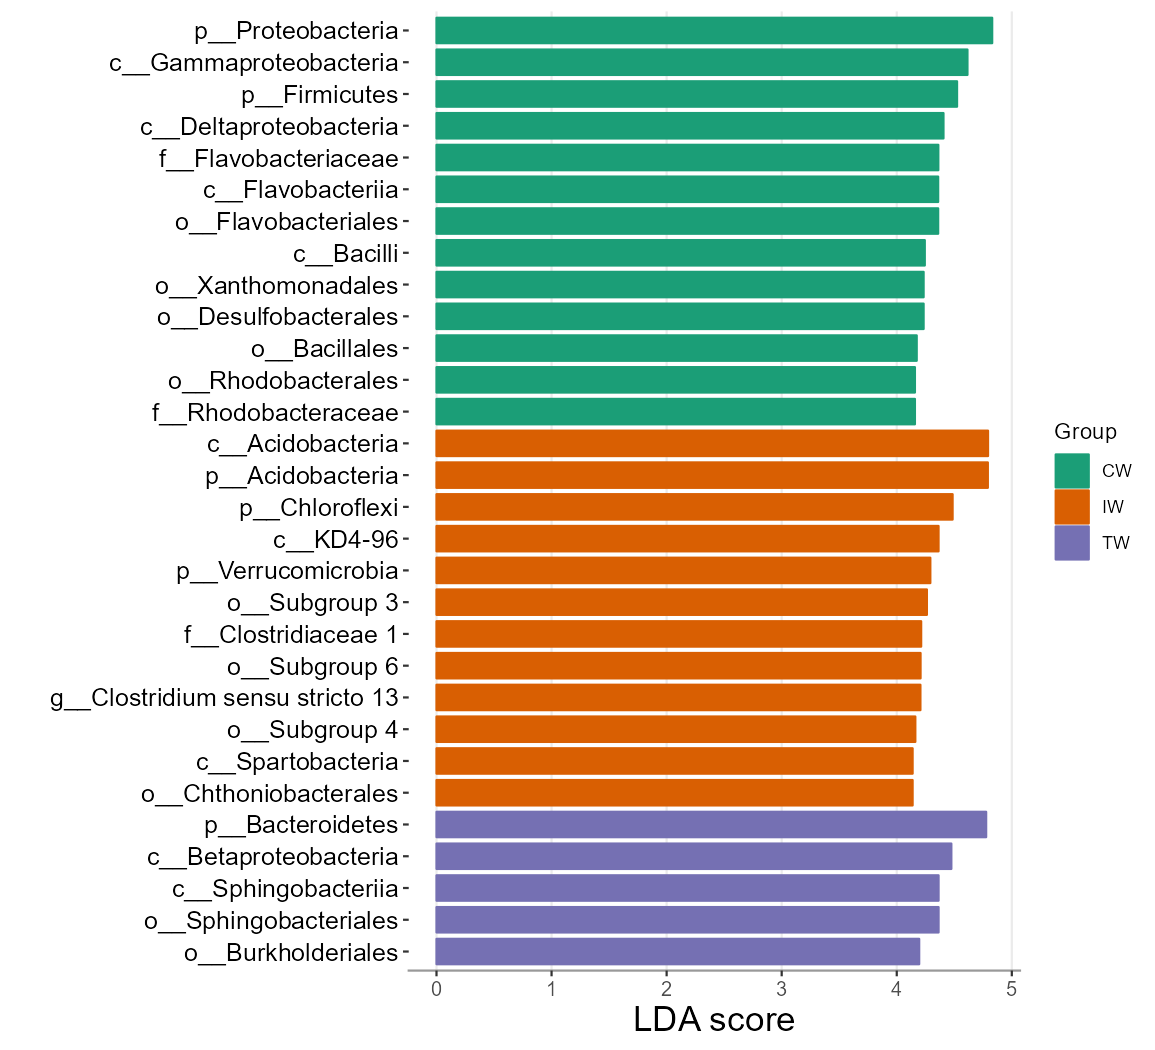
\includegraphics[width=700px]{Images/trans_diff_lefse_bar} \end{center}

\begin{Shaded}
\begin{Highlighting}[]
\CommentTok{\# show part of the table}
\NormalTok{t1}\SpecialCharTok{$}\NormalTok{res\_diff[}\DecValTok{1}\SpecialCharTok{:}\DecValTok{5}\NormalTok{, }\FunctionTok{c}\NormalTok{(}\DecValTok{1}\NormalTok{, }\DecValTok{3}\NormalTok{, }\DecValTok{4}\NormalTok{, }\DecValTok{6}\NormalTok{)]}
\end{Highlighting}
\end{Shaded}

\begin{longtable}[]{@{}
  >{\centering\arraybackslash}p{(\columnwidth - 6\tabcolsep) * \real{0.6627}}
  >{\centering\arraybackslash}p{(\columnwidth - 6\tabcolsep) * \real{0.0964}}
  >{\centering\arraybackslash}p{(\columnwidth - 6\tabcolsep) * \real{0.0964}}
  >{\centering\arraybackslash}p{(\columnwidth - 6\tabcolsep) * \real{0.1446}}@{}}
\toprule()
\begin{minipage}[b]{\linewidth}\centering
Taxa
\end{minipage} & \begin{minipage}[b]{\linewidth}\centering
Group
\end{minipage} & \begin{minipage}[b]{\linewidth}\centering
LDA
\end{minipage} & \begin{minipage}[b]{\linewidth}\centering
P.adj
\end{minipage} \\
\midrule()
\endhead
k\_\_Bacteria\textbar p\_\_Proteobacteria & CW & 4.837 & 1.076e-09 \\
k\_\_Bacteria\textbar p\_\_Acidobacteria & IW & 4.797 & 2.955e-10 \\
k\_\_Bacteria\textbar p\_\_Acidobacteria\textbar c\_\_Acidobacteria & IW & 4.797 & 6.946e-11 \\
k\_\_Bacteria\textbar p\_\_Bacteroidetes & TW & 4.782 & 1.529e-08 \\
k\_\_Bacteria\textbar p\_\_Proteobacteria\textbar c\_\_Gammaproteobacteria & CW & 4.613 & 2.911e-10 \\
\bottomrule()
\end{longtable}

Then, we plot the abundance of biomarkers detected by LEfSe.

\begin{Shaded}
\begin{Highlighting}[]
\NormalTok{t1}\SpecialCharTok{$}\FunctionTok{plot\_diff\_abund}\NormalTok{(}\AttributeTok{use\_number =} \DecValTok{1}\SpecialCharTok{:}\DecValTok{30}\NormalTok{, }\AttributeTok{group\_order =} \FunctionTok{c}\NormalTok{(}\StringTok{"CW"}\NormalTok{, }\StringTok{"IW"}\NormalTok{, }\StringTok{"TW"}\NormalTok{))}
\end{Highlighting}
\end{Shaded}

\begin{center}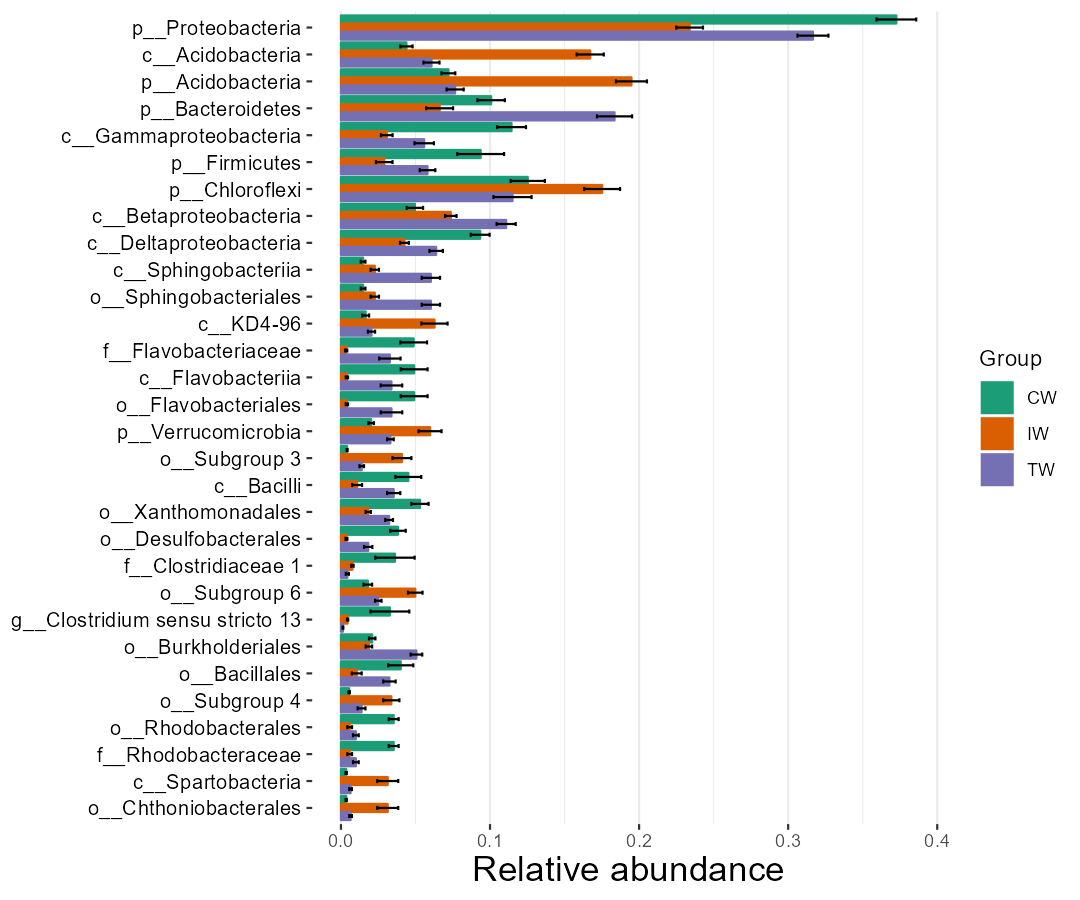
\includegraphics[width=650px]{Images/trans_diff_lefse_abund} \end{center}

Then, we show the cladogram of the differential features in the taxonomic tree.
There are too many taxa in this dataset.
As an example, we only select the highest 200 abundant taxa in the tree and 50 differential features.
We only show the full taxonomic label at Phylum level and use letters at other levels to reduce the text overlap.
\textbf{Note that if an error occurs in this function, the reason with a high probability is the chaotic taxonomy in the user's data}.
\textbf{Please see the \texttt{tidy\_taxonomy} function of microtable class part to solve this issue.}

\begin{Shaded}
\begin{Highlighting}[]
\CommentTok{\# clade\_label\_level 5 represent phylum level in this analysis}
\CommentTok{\# require ggtree package}
\NormalTok{t1}\SpecialCharTok{$}\FunctionTok{plot\_diff\_cladogram}\NormalTok{(}\AttributeTok{use\_taxa\_num =} \DecValTok{200}\NormalTok{, }\AttributeTok{use\_feature\_num =} \DecValTok{50}\NormalTok{, }\AttributeTok{clade\_label\_level =} \DecValTok{5}\NormalTok{, }\AttributeTok{group\_order =} \FunctionTok{c}\NormalTok{(}\StringTok{"CW"}\NormalTok{, }\StringTok{"IW"}\NormalTok{, }\StringTok{"TW"}\NormalTok{))}
\end{Highlighting}
\end{Shaded}

\begin{center}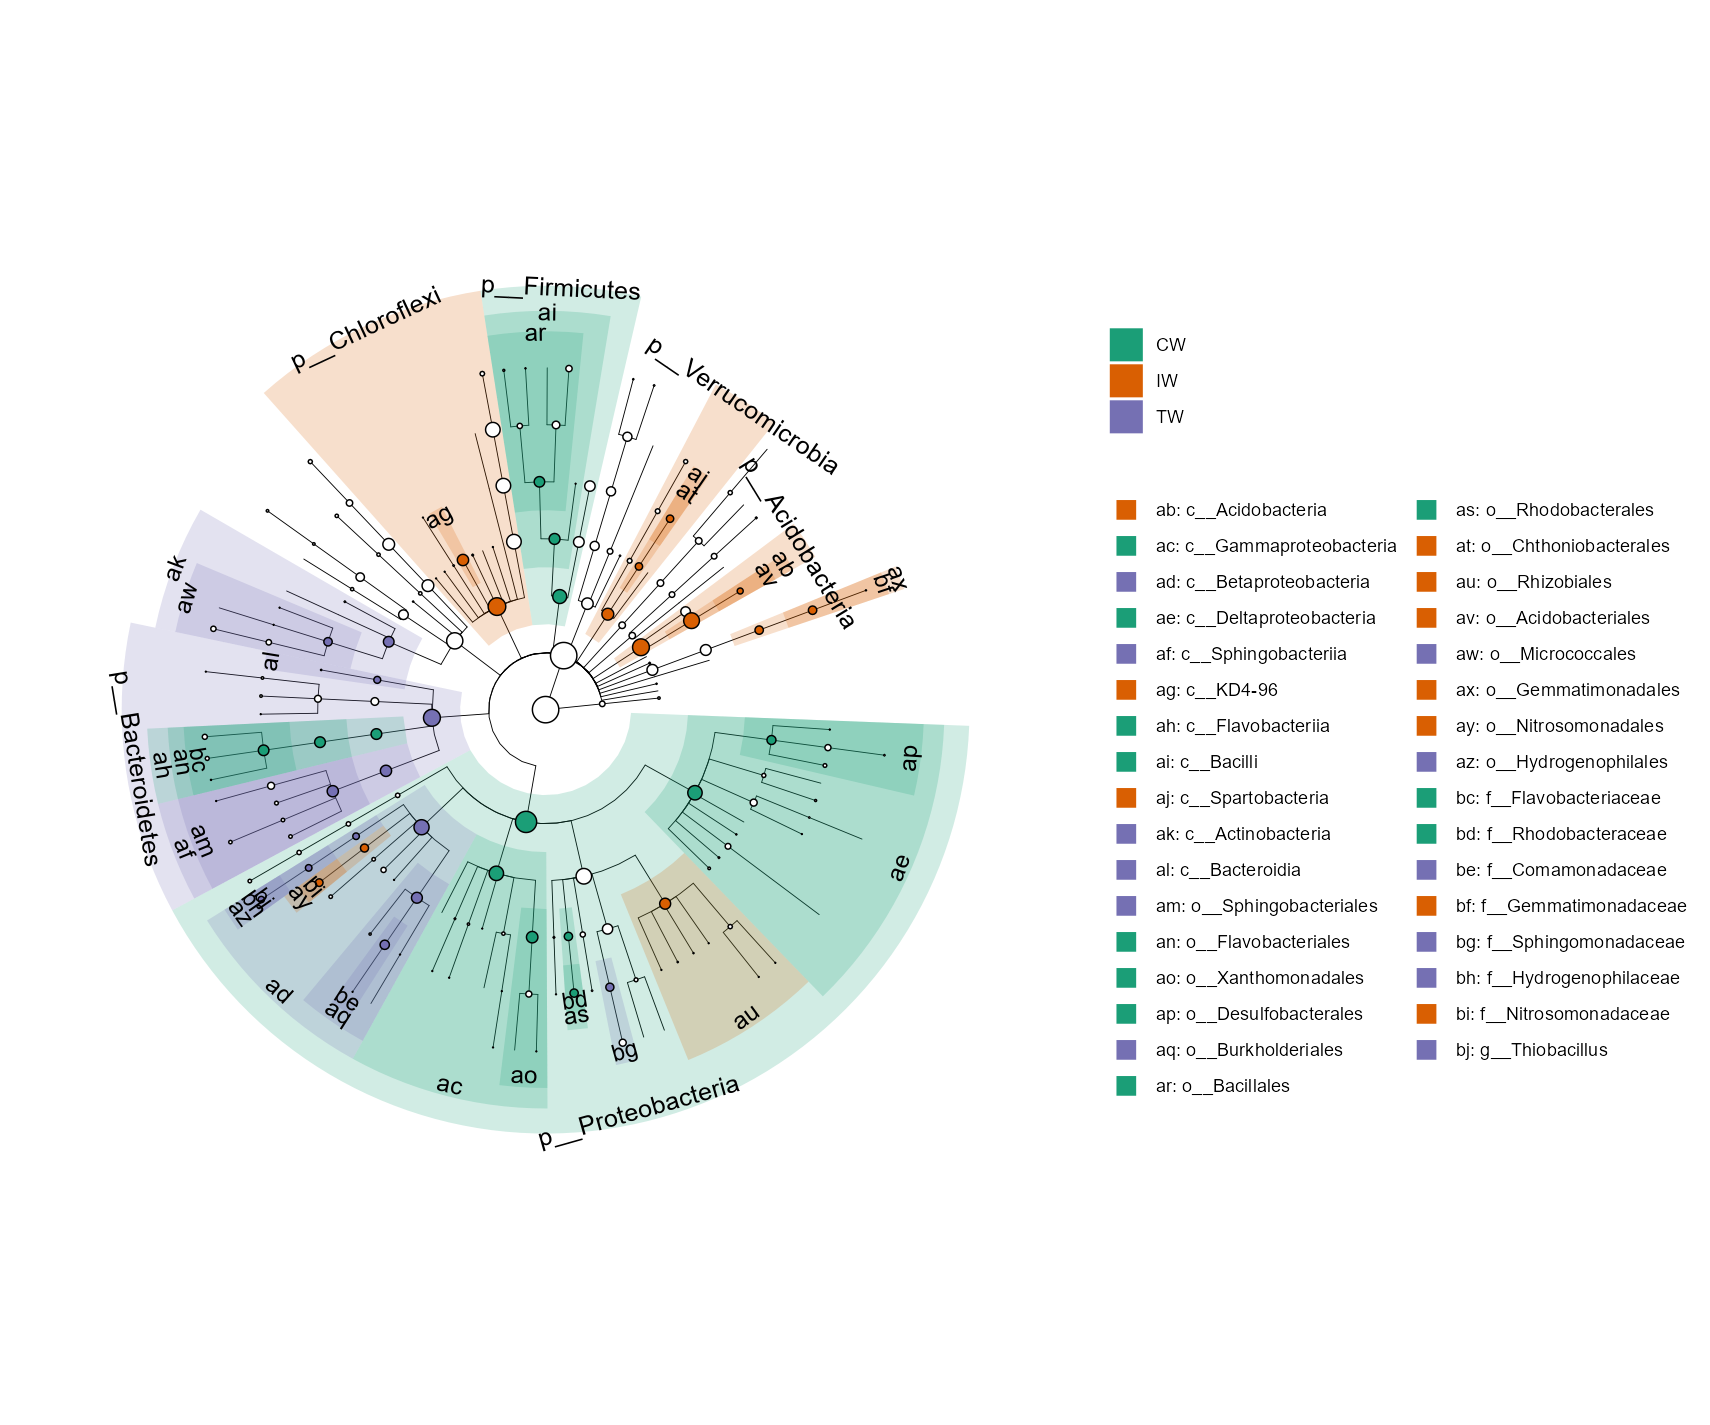
\includegraphics[width=1000px]{Images/trans_diff_lefse_cladogram} \end{center}

There may be a problem related with the taxonomic labels in the plot.
When there are too many levels shown, the taxonomic labels can have too much overlap.
However, if only Phylum labels are indicated, the taxa in the legend with marked letters are too many.
At this time, taxa can be manually choosed to show like the following operation.

\begin{Shaded}
\begin{Highlighting}[]
\CommentTok{\# choose some taxa according to the positions in the previous picture; those taxa labels have minimum overlap}
\NormalTok{use\_labels }\OtherTok{\textless{}{-}} \FunctionTok{c}\NormalTok{(}\StringTok{"c\_\_Deltaproteobacteria"}\NormalTok{, }\StringTok{"c\_\_Actinobacteria"}\NormalTok{, }\StringTok{"o\_\_Rhizobiales"}\NormalTok{, }\StringTok{"p\_\_Proteobacteria"}\NormalTok{, }\StringTok{"p\_\_Bacteroidetes"}\NormalTok{, }
    \StringTok{"o\_\_Micrococcales"}\NormalTok{, }\StringTok{"p\_\_Acidobacteria"}\NormalTok{, }\StringTok{"p\_\_Verrucomicrobia"}\NormalTok{, }\StringTok{"p\_\_Firmicutes"}\NormalTok{, }
    \StringTok{"p\_\_Chloroflexi"}\NormalTok{, }\StringTok{"c\_\_Acidobacteria"}\NormalTok{, }\StringTok{"c\_\_Gammaproteobacteria"}\NormalTok{, }\StringTok{"c\_\_Betaproteobacteria"}\NormalTok{, }\StringTok{"c\_\_KD4{-}96"}\NormalTok{,}
    \StringTok{"c\_\_Bacilli"}\NormalTok{, }\StringTok{"o\_\_Gemmatimonadales"}\NormalTok{, }\StringTok{"f\_\_Gemmatimonadaceae"}\NormalTok{, }\StringTok{"o\_\_Bacillales"}\NormalTok{, }\StringTok{"o\_\_Rhodobacterales"}\NormalTok{)}
\CommentTok{\# then use parameter select\_show\_labels to show}
\NormalTok{t1}\SpecialCharTok{$}\FunctionTok{plot\_diff\_cladogram}\NormalTok{(}\AttributeTok{use\_taxa\_num =} \DecValTok{200}\NormalTok{, }\AttributeTok{use\_feature\_num =} \DecValTok{50}\NormalTok{, }\AttributeTok{select\_show\_labels =}\NormalTok{ use\_labels)}
\CommentTok{\# Now we can see that more taxa names appear in the tree}
\end{Highlighting}
\end{Shaded}

\begin{center}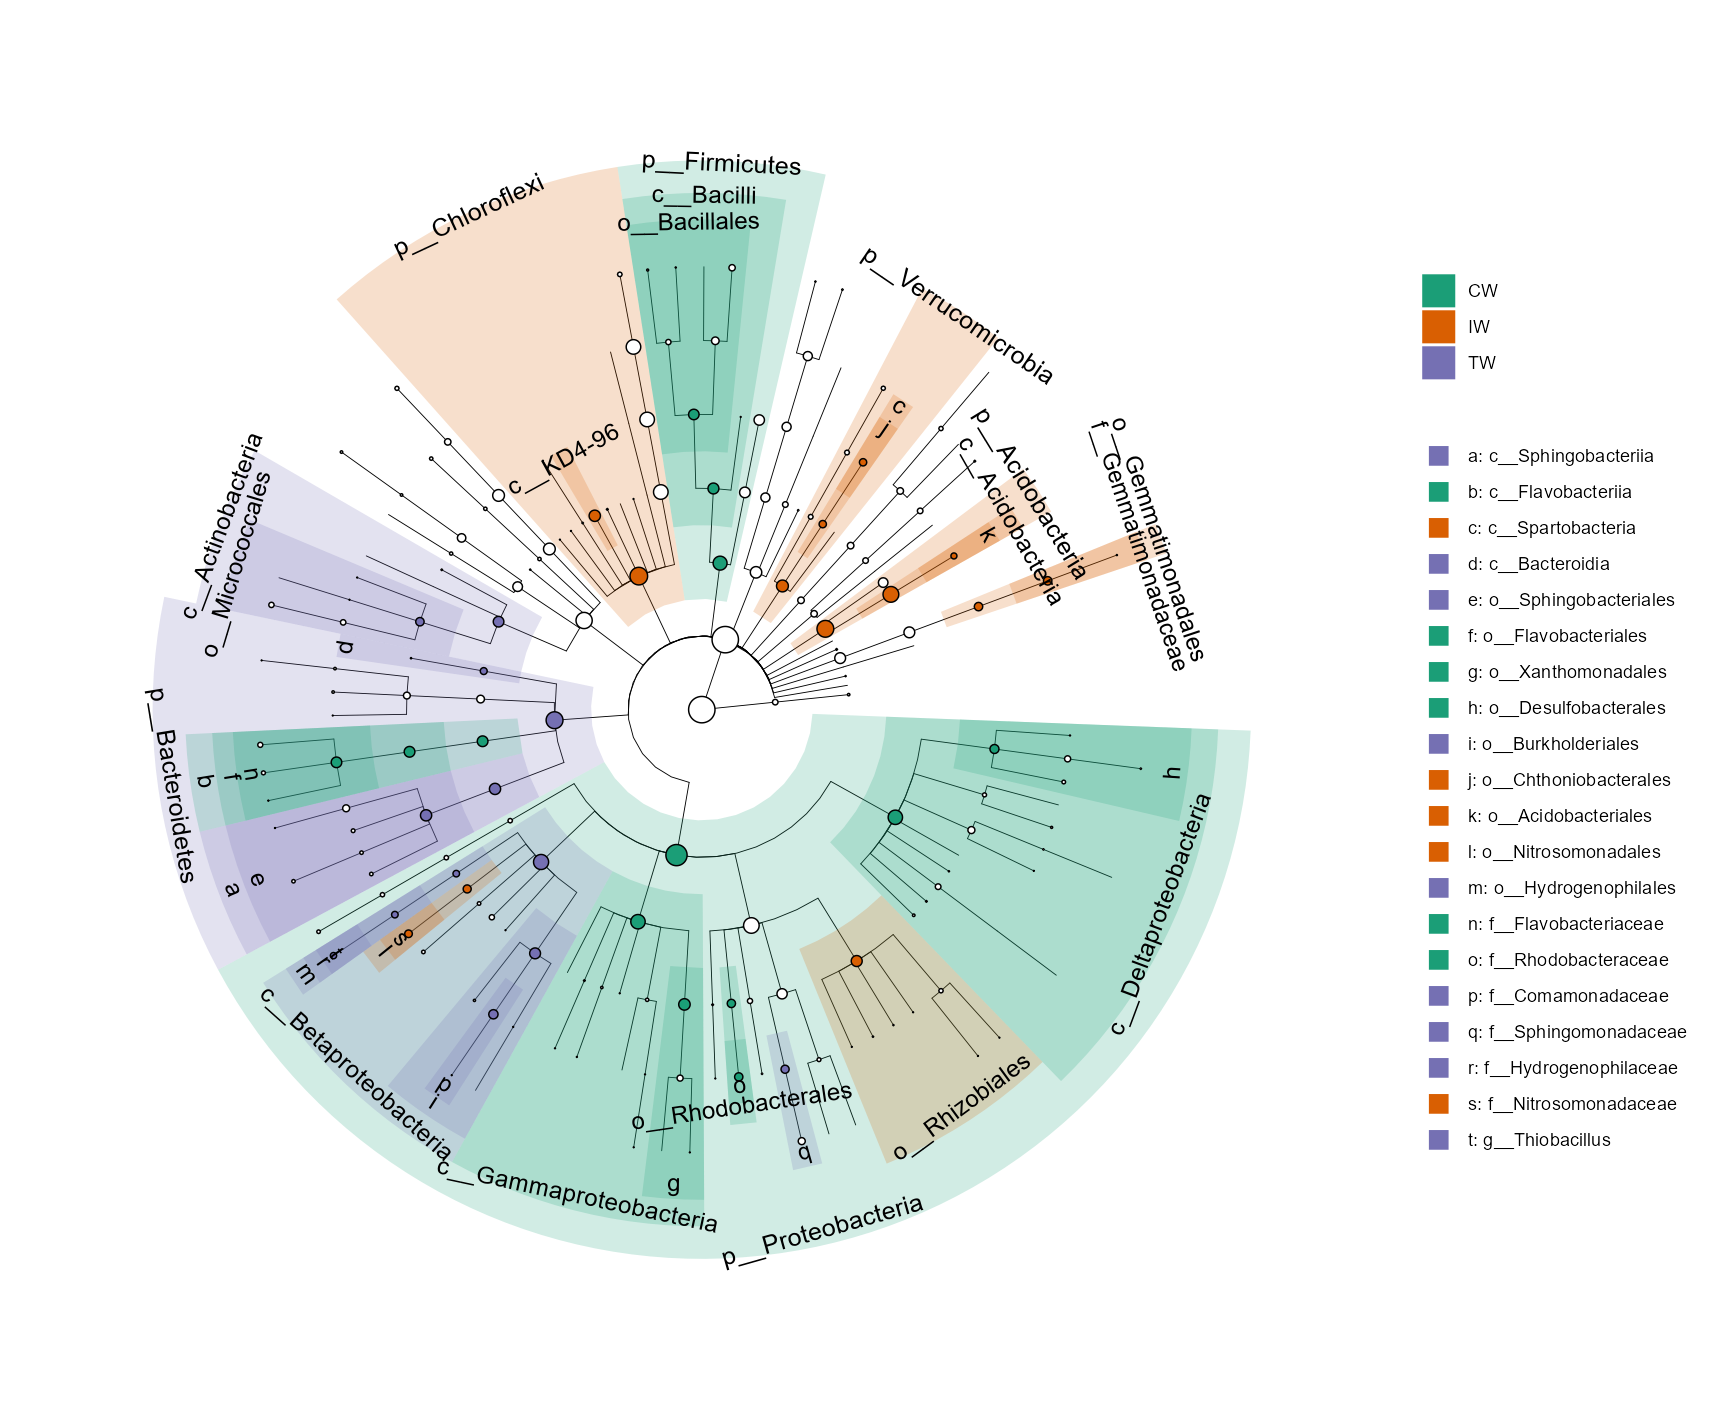
\includegraphics[width=1000px]{Images/trans_diff_lefse_cladogram_1} \end{center}

The `rf' method depends on the random forest\citep{Beck_Machine_2014, Yatsunenko_Human_2012} and the non-parametric test.
The current method can calculate random forest by bootstrapping like the method in LEfSe and only use the significant features.
MeanDecreaseGini is selected as the indicator value in the analysis.

\begin{Shaded}
\begin{Highlighting}[]
\CommentTok{\# use Genus level for parameter taxa\_level, if you want to use all taxa, change to "all"}
\CommentTok{\# nresam = 1 and boots = 1 represent no bootstrapping and use all samples directly}
\NormalTok{t1 }\OtherTok{\textless{}{-}}\NormalTok{ trans\_diff}\SpecialCharTok{$}\FunctionTok{new}\NormalTok{(}\AttributeTok{dataset =}\NormalTok{ dataset, }\AttributeTok{method =} \StringTok{"rf"}\NormalTok{, }\AttributeTok{group =} \StringTok{"Group"}\NormalTok{, }\AttributeTok{taxa\_level =} \StringTok{"Genus"}\NormalTok{)}
\CommentTok{\# plot the MeanDecreaseGini bar}
\CommentTok{\# group\_order is designed to sort the groups}
\NormalTok{g1 }\OtherTok{\textless{}{-}}\NormalTok{ t1}\SpecialCharTok{$}\FunctionTok{plot\_diff\_bar}\NormalTok{(}\AttributeTok{use\_number =} \DecValTok{1}\SpecialCharTok{:}\DecValTok{20}\NormalTok{, }\AttributeTok{group\_order =} \FunctionTok{c}\NormalTok{(}\StringTok{"TW"}\NormalTok{, }\StringTok{"CW"}\NormalTok{, }\StringTok{"IW"}\NormalTok{))}
\CommentTok{\# plot the abundance using same taxa in g1}
\NormalTok{g2 }\OtherTok{\textless{}{-}}\NormalTok{ t1}\SpecialCharTok{$}\FunctionTok{plot\_diff\_abund}\NormalTok{(}\AttributeTok{group\_order =} \FunctionTok{c}\NormalTok{(}\StringTok{"TW"}\NormalTok{, }\StringTok{"CW"}\NormalTok{, }\StringTok{"IW"}\NormalTok{), }\AttributeTok{select\_taxa =}\NormalTok{ t1}\SpecialCharTok{$}\NormalTok{plot\_diff\_bar\_taxa)}
\CommentTok{\# now the y axis in g1 and g2 is same, so we can merge them}
\CommentTok{\# remove g1 legend; remove g2 y axis text and ticks}
\NormalTok{g1 }\OtherTok{\textless{}{-}}\NormalTok{ g1 }\SpecialCharTok{+} \FunctionTok{theme}\NormalTok{(}\AttributeTok{legend.position =} \StringTok{"none"}\NormalTok{)}
\NormalTok{g2 }\OtherTok{\textless{}{-}}\NormalTok{ g2 }\SpecialCharTok{+} \FunctionTok{theme}\NormalTok{(}\AttributeTok{axis.text.y =} \FunctionTok{element\_blank}\NormalTok{(), }\AttributeTok{axis.ticks.y =} \FunctionTok{element\_blank}\NormalTok{())}
\NormalTok{gridExtra}\SpecialCharTok{::}\FunctionTok{grid.arrange}\NormalTok{(g1, g2, }\AttributeTok{ncol =} \DecValTok{2}\NormalTok{, }\AttributeTok{nrow =} \DecValTok{1}\NormalTok{, }\AttributeTok{widths =} \FunctionTok{c}\NormalTok{(}\DecValTok{2}\NormalTok{, }\FloatTok{1.7}\NormalTok{))}
\end{Highlighting}
\end{Shaded}

\begin{center}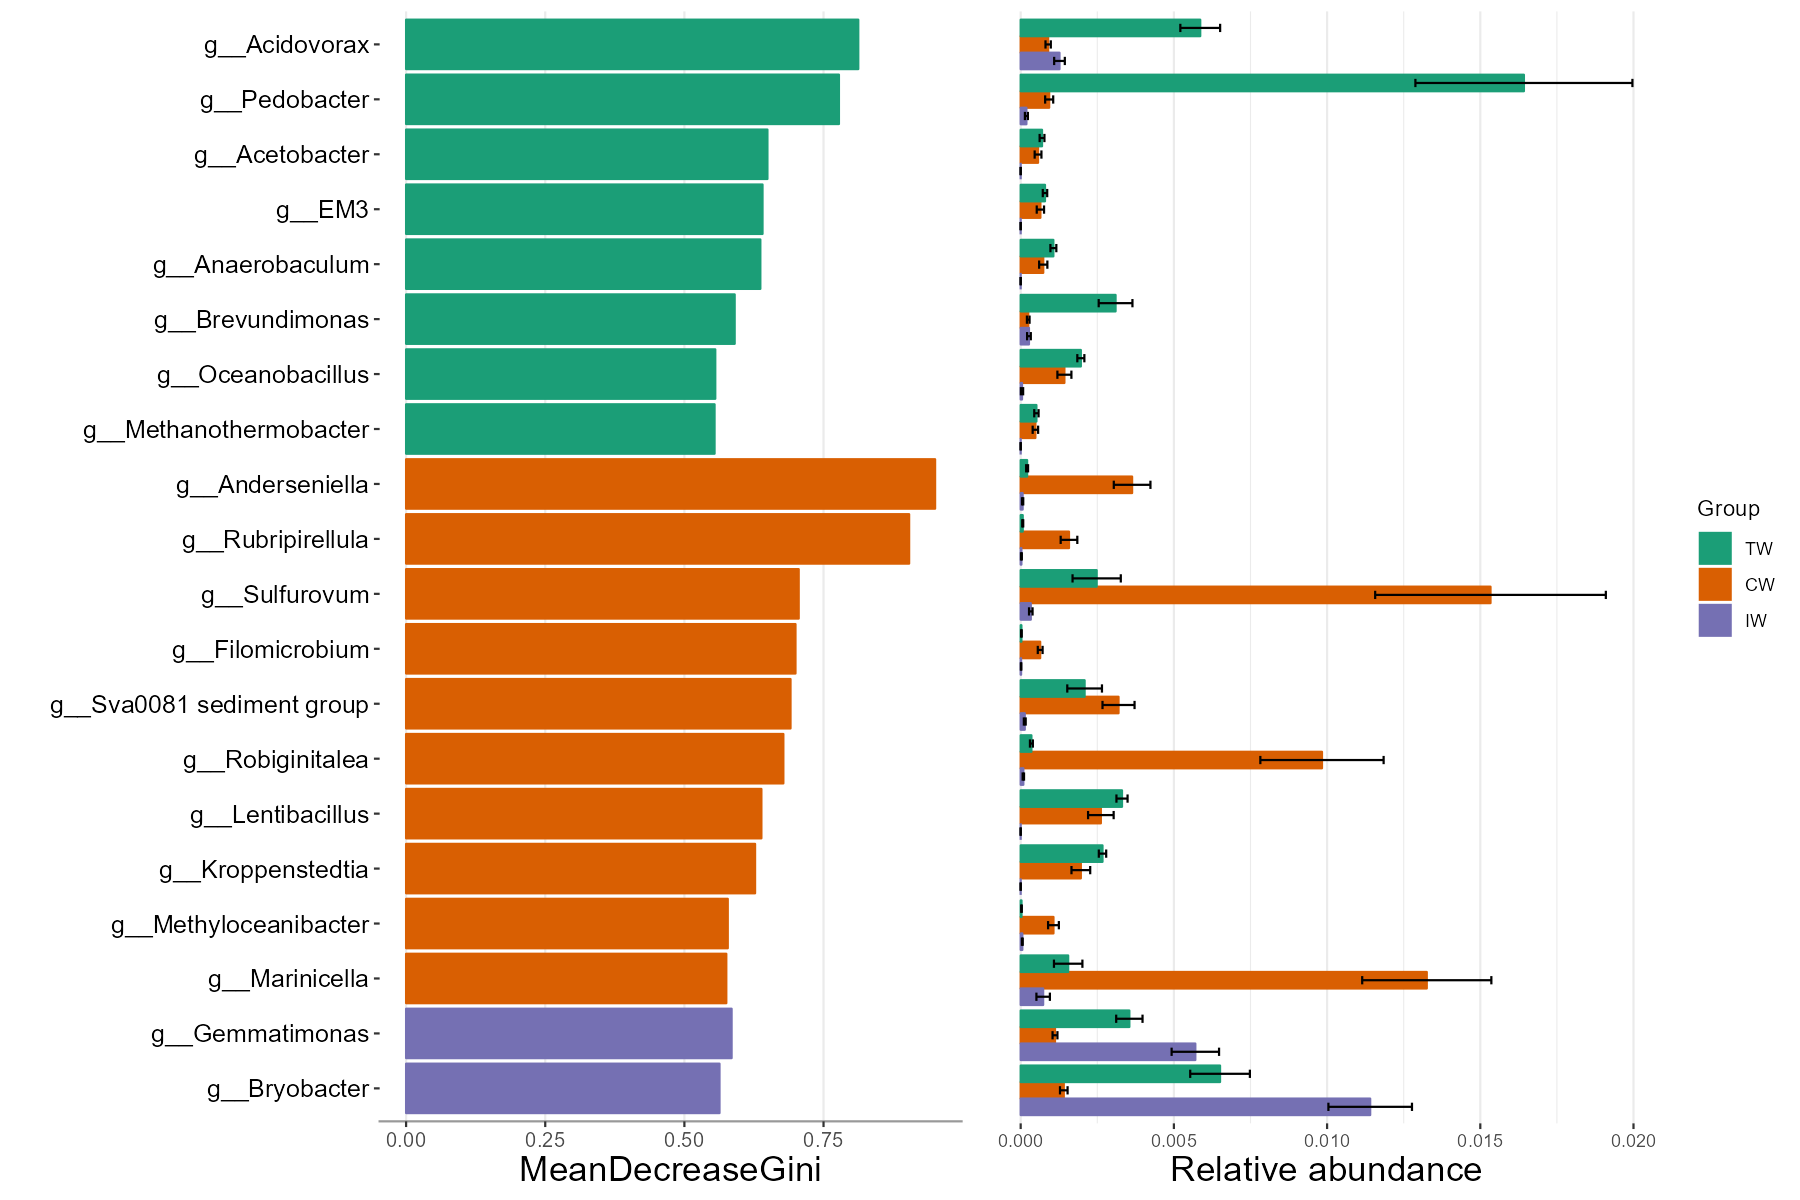
\includegraphics[width=800px]{Images/trans_diff_rf_diff_abund} \end{center}

The significance label can also be added in the abundance plot controlled by add\_sig parameter and other related parameters.
Now adding labels supports all the differential test methods.

\begin{Shaded}
\begin{Highlighting}[]
\NormalTok{t1 }\OtherTok{\textless{}{-}}\NormalTok{ trans\_diff}\SpecialCharTok{$}\FunctionTok{new}\NormalTok{(}\AttributeTok{dataset =}\NormalTok{ dataset, }\AttributeTok{method =} \StringTok{"wilcox"}\NormalTok{, }\AttributeTok{group =} \StringTok{"Group"}\NormalTok{, }\AttributeTok{taxa\_level =} \StringTok{"Genus"}\NormalTok{, }\AttributeTok{filter\_thres =} \FloatTok{0.001}\NormalTok{)}
\CommentTok{\# filter something not needed to show}
\NormalTok{t1}\SpecialCharTok{$}\NormalTok{res\_diff }\SpecialCharTok{\%\textless{}\textgreater{}\%} \FunctionTok{subset}\NormalTok{(Significance }\SpecialCharTok{\%in\%} \StringTok{"***"}\NormalTok{)}
\NormalTok{t1}\SpecialCharTok{$}\FunctionTok{plot\_diff\_abund}\NormalTok{(}\AttributeTok{use\_number =} \DecValTok{1}\SpecialCharTok{:}\DecValTok{10}\NormalTok{, }\AttributeTok{add\_sig =}\NormalTok{ T, }\AttributeTok{add\_sig\_label =} \StringTok{"Significance"}\NormalTok{)}
\end{Highlighting}
\end{Shaded}

\begin{center}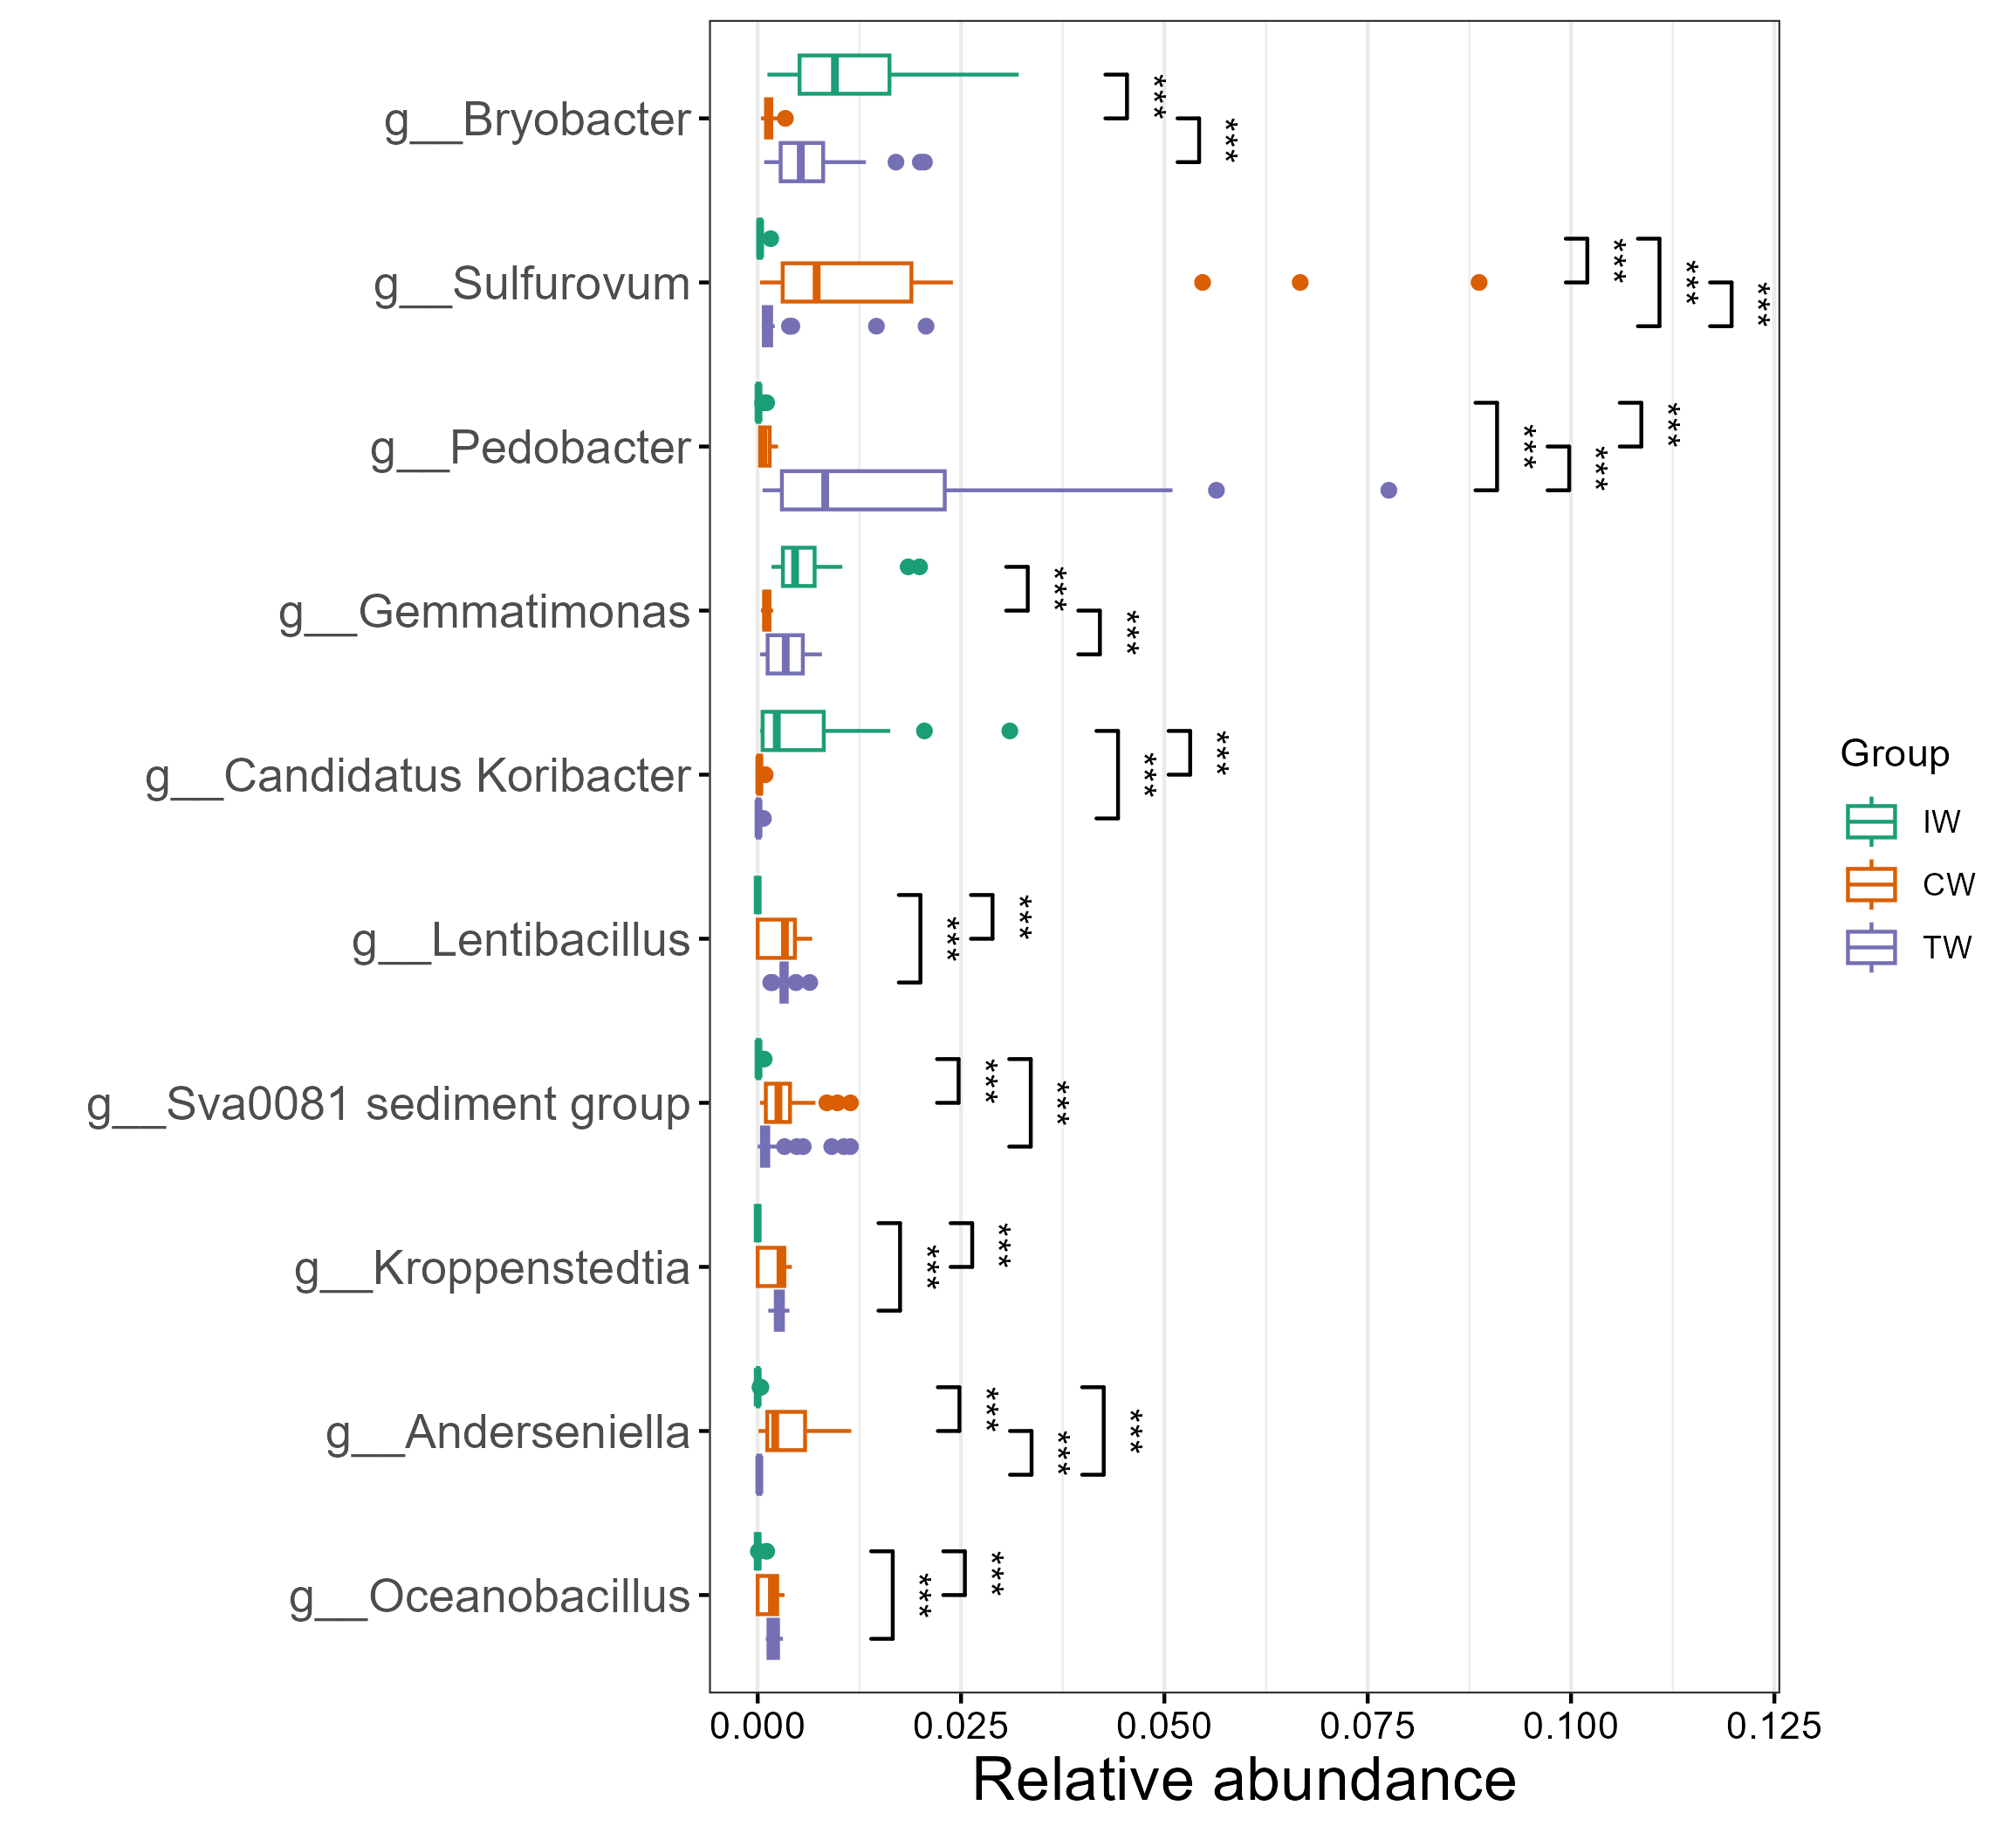
\includegraphics[width=700px]{Images/trans_diff_siglabel_wilcox} \end{center}

\begin{Shaded}
\begin{Highlighting}[]
\NormalTok{t1 }\OtherTok{\textless{}{-}}\NormalTok{ trans\_diff}\SpecialCharTok{$}\FunctionTok{new}\NormalTok{(}\AttributeTok{dataset =}\NormalTok{ dataset, }\AttributeTok{method =} \StringTok{"anova"}\NormalTok{, }\AttributeTok{group =} \StringTok{"Group"}\NormalTok{, }\AttributeTok{taxa\_level =} \StringTok{"Genus"}\NormalTok{, }\AttributeTok{filter\_thres =} \FloatTok{0.001}\NormalTok{)}
\NormalTok{t1}\SpecialCharTok{$}\FunctionTok{plot\_diff\_abund}\NormalTok{(}\AttributeTok{use\_number =} \DecValTok{1}\SpecialCharTok{:}\DecValTok{10}\NormalTok{, }\AttributeTok{add\_sig =}\NormalTok{ T, }\AttributeTok{coord\_flip =}\NormalTok{ F)}
\end{Highlighting}
\end{Shaded}

\begin{center}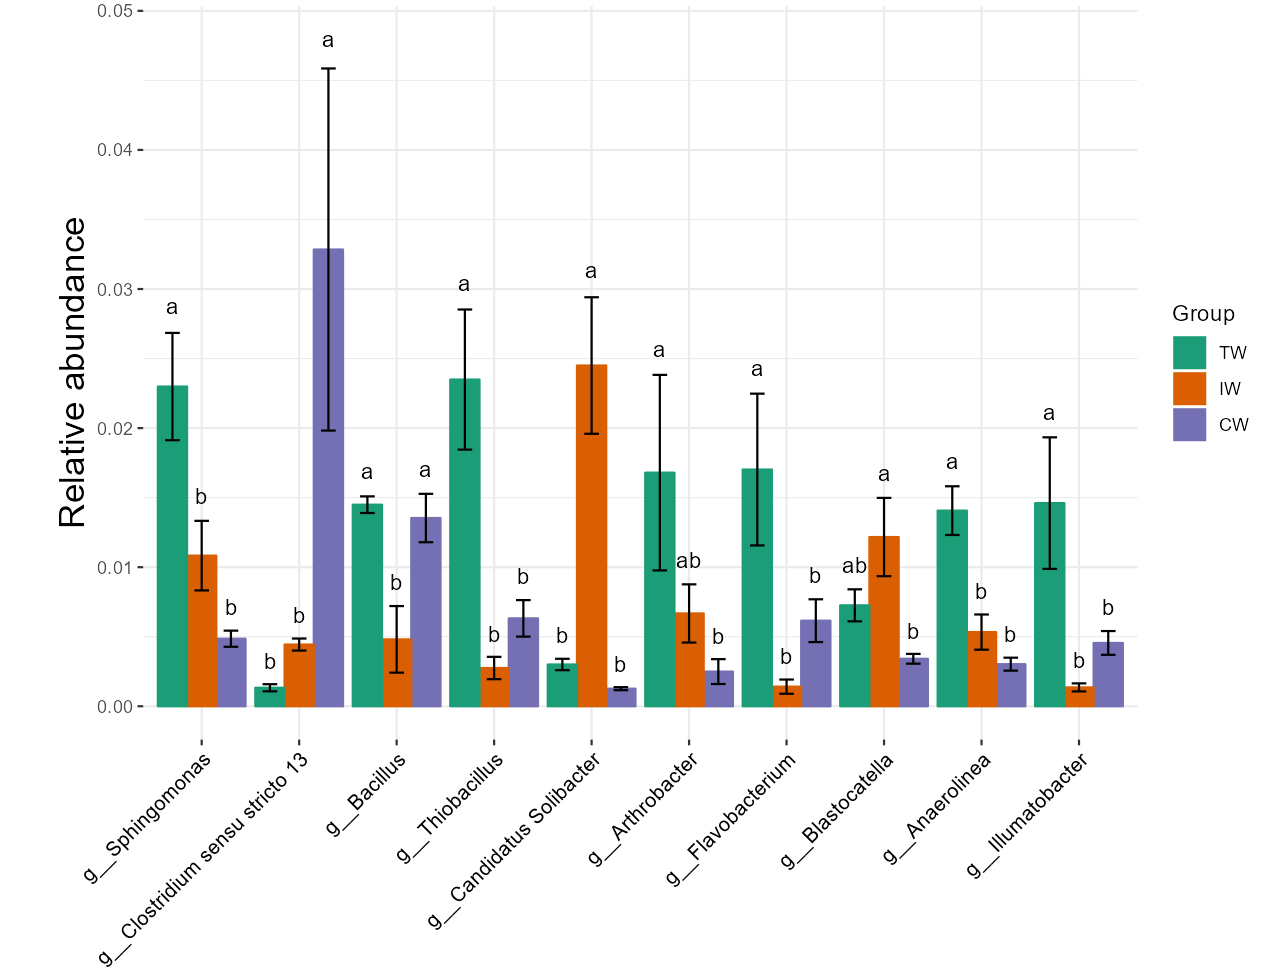
\includegraphics[width=700px]{Images/trans_diff_siglabel_anova} \end{center}

Metastat depends on the permutations and t-test and performs well on the sparse data for paired groups test.

\begin{Shaded}
\begin{Highlighting}[]
\CommentTok{\# metastat analysis at Genus level}
\NormalTok{t1 }\OtherTok{\textless{}{-}}\NormalTok{ trans\_diff}\SpecialCharTok{$}\FunctionTok{new}\NormalTok{(}\AttributeTok{dataset =}\NormalTok{ dataset, }\AttributeTok{method =} \StringTok{"metastat"}\NormalTok{, }\AttributeTok{group =} \StringTok{"Group"}\NormalTok{, }\AttributeTok{taxa\_level =} \StringTok{"Genus"}\NormalTok{)}
\CommentTok{\# t1$res\_diff is the differential test result}
\CommentTok{\# t1$res\_abund is the group abundance}
\end{Highlighting}
\end{Shaded}

Because the example `Group' in sample\_table has three groups,
the metastat can run the comparisons for each paired group. So there are three pairs in t1\$res\_diff\$Comparison.
For the abundance plotting, the user should use select\_group to select the required pair.

\begin{Shaded}
\begin{Highlighting}[]
\CommentTok{\# select\_group should be one of groups in t1$res\_diff$Comparison}
\NormalTok{t1}\SpecialCharTok{$}\FunctionTok{plot\_diff\_abund}\NormalTok{(}\AttributeTok{use\_number =} \DecValTok{1}\SpecialCharTok{:}\DecValTok{20}\NormalTok{, }\AttributeTok{select\_group =} \StringTok{"CW {-} TW"}\NormalTok{, }\AttributeTok{coord\_flip =}\NormalTok{ F)}
\end{Highlighting}
\end{Shaded}

\begin{center}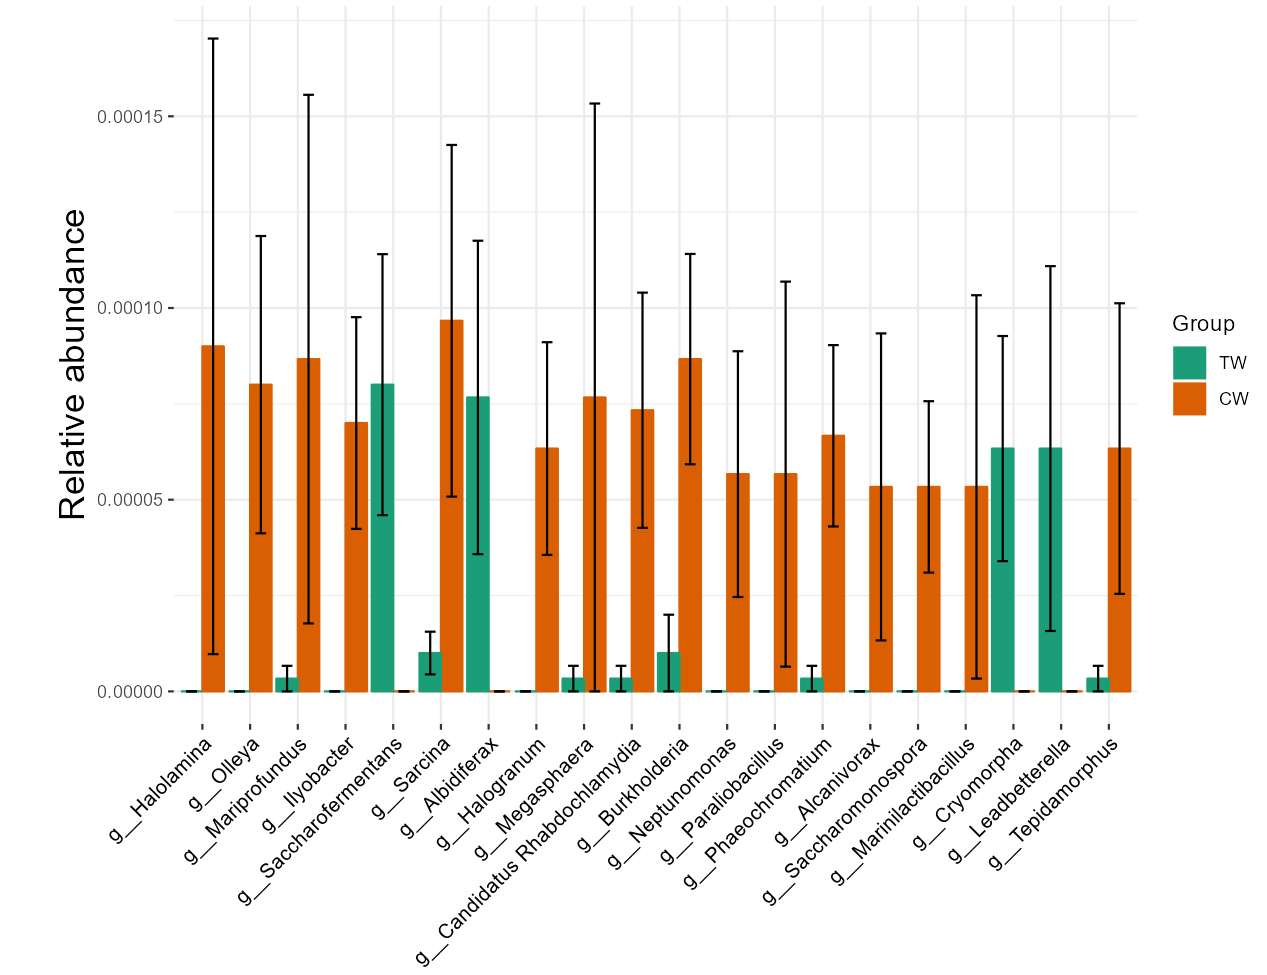
\includegraphics[width=650px]{Images/trans_diff_metastat_1} \end{center}

The following are the examples for the methods `KW', `KW\_dunn', `wilcox', `t.test' and `anova'.

\begin{Shaded}
\begin{Highlighting}[]
\CommentTok{\# Kruskal{-}Wallis Rank Sum Test for all groups (\textgreater{}= 2)}
\NormalTok{t1 }\OtherTok{\textless{}{-}}\NormalTok{ trans\_diff}\SpecialCharTok{$}\FunctionTok{new}\NormalTok{(}\AttributeTok{dataset =}\NormalTok{ dataset, }\AttributeTok{method =} \StringTok{"KW"}\NormalTok{, }\AttributeTok{group =} \StringTok{"Group"}\NormalTok{, }\AttributeTok{taxa\_level =} \StringTok{"all"}\NormalTok{, }\AttributeTok{filter\_thres =} \FloatTok{0.001}\NormalTok{)}
\NormalTok{t1}\SpecialCharTok{$}\FunctionTok{plot\_diff\_abund}\NormalTok{(}\AttributeTok{use\_number =} \DecValTok{1}\SpecialCharTok{:}\DecValTok{20}\NormalTok{)}
\CommentTok{\# Dunn\textquotesingle{}s Kruskal{-}Wallis Multiple Comparisons when group number \textgreater{} 2; require FSA package}
\NormalTok{t1 }\OtherTok{\textless{}{-}}\NormalTok{ trans\_diff}\SpecialCharTok{$}\FunctionTok{new}\NormalTok{(}\AttributeTok{dataset =}\NormalTok{ dataset, }\AttributeTok{method =} \StringTok{"KW\_dunn"}\NormalTok{, }\AttributeTok{group =} \StringTok{"Group"}\NormalTok{, }\AttributeTok{taxa\_level =} \StringTok{"Genus"}\NormalTok{, }\AttributeTok{filter\_thres =} \FloatTok{0.0001}\NormalTok{)}
\NormalTok{t1}\SpecialCharTok{$}\FunctionTok{plot\_diff\_abund}\NormalTok{(}\AttributeTok{use\_number =} \DecValTok{1}\SpecialCharTok{:}\DecValTok{10}\NormalTok{, }\AttributeTok{add\_sig =}\NormalTok{ T, }\AttributeTok{coord\_flip =}\NormalTok{ F)}
\CommentTok{\# Wilcoxon Rank Sum and Signed Rank Tests for all paired groups}
\NormalTok{t1 }\OtherTok{\textless{}{-}}\NormalTok{ trans\_diff}\SpecialCharTok{$}\FunctionTok{new}\NormalTok{(}\AttributeTok{dataset =}\NormalTok{ dataset, }\AttributeTok{method =} \StringTok{"wilcox"}\NormalTok{, }\AttributeTok{group =} \StringTok{"Group"}\NormalTok{, }\AttributeTok{taxa\_level =} \StringTok{"Genus"}\NormalTok{, }\AttributeTok{filter\_thres =} \FloatTok{0.001}\NormalTok{)}
\NormalTok{t1}\SpecialCharTok{$}\FunctionTok{plot\_diff\_bar}\NormalTok{(}\AttributeTok{use\_number =} \DecValTok{1}\SpecialCharTok{:}\DecValTok{20}\NormalTok{, }\AttributeTok{select\_group =} \StringTok{"CW {-} TW"}\NormalTok{)}
\NormalTok{t1}\SpecialCharTok{$}\FunctionTok{plot\_diff\_abund}\NormalTok{(}\AttributeTok{use\_number =} \DecValTok{1}\SpecialCharTok{:}\DecValTok{20}\NormalTok{, }\AttributeTok{select\_group =} \StringTok{"CW {-} TW"}\NormalTok{, }\AttributeTok{group\_order =} \FunctionTok{c}\NormalTok{(}\StringTok{"TW"}\NormalTok{, }\StringTok{"CW"}\NormalTok{))}
\CommentTok{\# t.test}
\NormalTok{t1 }\OtherTok{\textless{}{-}}\NormalTok{ trans\_diff}\SpecialCharTok{$}\FunctionTok{new}\NormalTok{(}\AttributeTok{dataset =}\NormalTok{ dataset, }\AttributeTok{method =} \StringTok{"t.test"}\NormalTok{, }\AttributeTok{group =} \StringTok{"Group"}\NormalTok{, }\AttributeTok{taxa\_level =} \StringTok{"all"}\NormalTok{, }\AttributeTok{filter\_thres =} \FloatTok{0.001}\NormalTok{)}
\CommentTok{\# anova}
\NormalTok{t1 }\OtherTok{\textless{}{-}}\NormalTok{ trans\_diff}\SpecialCharTok{$}\FunctionTok{new}\NormalTok{(}\AttributeTok{dataset =}\NormalTok{ dataset, }\AttributeTok{method =} \StringTok{"anova"}\NormalTok{, }\AttributeTok{group =} \StringTok{"Group"}\NormalTok{, }\AttributeTok{taxa\_level =} \StringTok{"Phylum"}\NormalTok{, }\AttributeTok{filter\_thres =} \FloatTok{0.001}\NormalTok{)}
\FunctionTok{head}\NormalTok{(t1}\SpecialCharTok{$}\NormalTok{res\_diff)}
\end{Highlighting}
\end{Shaded}

The method `metagenomeSeq' \citep{Paulson_Differential_2013} and `ancombc2' \citep{Lin_Analysis_2020} depend on the metagenomeSeq package and ANCOMBC package, respectively.
The method `ALDEx2\_t' and `ALDEx2\_kw' depend on the ALDEx2 package \citep{Fernandes_Unifying_2014}.
These three packages are all deposited on the Bioconductor.

\begin{Shaded}
\begin{Highlighting}[]
\CommentTok{\# zero{-}inflated log{-}normal model{-}based differential test method from metagenomeSeq package}
\CommentTok{\# If metagenomeSeq package is not installed, please first run: BiocManager::install("metagenomeSeq")}
\NormalTok{t1 }\OtherTok{\textless{}{-}}\NormalTok{ trans\_diff}\SpecialCharTok{$}\FunctionTok{new}\NormalTok{(}\AttributeTok{dataset =}\NormalTok{ dataset, }\AttributeTok{method =} \StringTok{"metagenomeSeq"}\NormalTok{, }\AttributeTok{group =} \StringTok{"Group"}\NormalTok{, }\AttributeTok{taxa\_level =} \StringTok{"Genus"}\NormalTok{)}
\NormalTok{t1 }\OtherTok{\textless{}{-}}\NormalTok{ trans\_diff}\SpecialCharTok{$}\FunctionTok{new}\NormalTok{(}\AttributeTok{dataset =}\NormalTok{ dataset, }\AttributeTok{method =} \StringTok{"metagenomeSeq"}\NormalTok{, }\AttributeTok{group =} \StringTok{"Group"}\NormalTok{, }\AttributeTok{taxa\_level =} \StringTok{"OTU"}\NormalTok{)}
\NormalTok{t1}\SpecialCharTok{$}\FunctionTok{plot\_diff\_abund}\NormalTok{(}\AttributeTok{use\_number =} \DecValTok{1}\SpecialCharTok{:}\DecValTok{30}\NormalTok{, }\AttributeTok{group\_order =} \FunctionTok{c}\NormalTok{(}\StringTok{"TW"}\NormalTok{, }\StringTok{"CW"}\NormalTok{, }\StringTok{"IW"}\NormalTok{))}
\NormalTok{t1}\SpecialCharTok{$}\FunctionTok{plot\_diff\_bar}\NormalTok{(}\AttributeTok{use\_number =} \DecValTok{1}\SpecialCharTok{:}\DecValTok{20}\NormalTok{)}
\end{Highlighting}
\end{Shaded}

\begin{Shaded}
\begin{Highlighting}[]
\CommentTok{\# \textquotesingle{}ALDEx2\_t\textquotesingle{} and \textquotesingle{}ALDEx2\_kw\textquotesingle{} methods; use ?trans\_diff to see detailed description of the methods}
\CommentTok{\# If ALDEx2 package is not installed, please first run: BiocManager::install("ALDEx2")}
\CommentTok{\# \textquotesingle{}ALDEx2\_t\textquotesingle{}}
\NormalTok{t1 }\OtherTok{\textless{}{-}}\NormalTok{ trans\_diff}\SpecialCharTok{$}\FunctionTok{new}\NormalTok{(}\AttributeTok{dataset =}\NormalTok{ dataset, }\AttributeTok{method =} \StringTok{"ALDEx2\_t"}\NormalTok{, }\AttributeTok{group =} \StringTok{"Group"}\NormalTok{, }\AttributeTok{taxa\_level =} \StringTok{"Phylum"}\NormalTok{)}
\NormalTok{t1}\SpecialCharTok{$}\FunctionTok{plot\_diff\_abund}\NormalTok{(}\AttributeTok{use\_number =} \DecValTok{1}\SpecialCharTok{:}\DecValTok{20}\NormalTok{, }\AttributeTok{group\_order =} \FunctionTok{c}\NormalTok{(}\StringTok{"TW"}\NormalTok{, }\StringTok{"CW"}\NormalTok{, }\StringTok{"IW"}\NormalTok{))}
\NormalTok{t1}\SpecialCharTok{$}\FunctionTok{plot\_diff\_abund}\NormalTok{(}\AttributeTok{use\_number =} \DecValTok{1}\SpecialCharTok{:}\DecValTok{20}\NormalTok{, }\AttributeTok{select\_group =} \StringTok{"CW {-} TW"}\NormalTok{)}
\NormalTok{t1}\SpecialCharTok{$}\FunctionTok{plot\_diff\_abund}\NormalTok{(}\AttributeTok{use\_number =} \DecValTok{1}\SpecialCharTok{:}\DecValTok{20}\NormalTok{, }\AttributeTok{select\_group =} \StringTok{"CW {-} TW"}\NormalTok{, }\AttributeTok{add\_sig =} \ConstantTok{TRUE}\NormalTok{)}
\NormalTok{t1 }\OtherTok{\textless{}{-}}\NormalTok{ trans\_diff}\SpecialCharTok{$}\FunctionTok{new}\NormalTok{(}\AttributeTok{dataset =}\NormalTok{ dataset, }\AttributeTok{method =} \StringTok{"ALDEx2\_t"}\NormalTok{, }\AttributeTok{group =} \StringTok{"Group"}\NormalTok{, }\AttributeTok{taxa\_level =} \StringTok{"OTU"}\NormalTok{, }\AttributeTok{filter\_thres =} \FloatTok{0.0005}\NormalTok{)}
\CommentTok{\# ALDEx2\_kw}
\NormalTok{t1 }\OtherTok{\textless{}{-}}\NormalTok{ trans\_diff}\SpecialCharTok{$}\FunctionTok{new}\NormalTok{(}\AttributeTok{dataset =}\NormalTok{ dataset, }\AttributeTok{method =} \StringTok{"ALDEx2\_kw"}\NormalTok{, }\AttributeTok{group =} \StringTok{"Group"}\NormalTok{, }\AttributeTok{taxa\_level =} \StringTok{"Phylum"}\NormalTok{)}
\NormalTok{t1}\SpecialCharTok{$}\FunctionTok{plot\_diff\_abund}\NormalTok{(}\AttributeTok{use\_number =} \DecValTok{1}\SpecialCharTok{:}\DecValTok{30}\NormalTok{, }\AttributeTok{group\_order =} \FunctionTok{c}\NormalTok{(}\StringTok{"TW"}\NormalTok{, }\StringTok{"CW"}\NormalTok{, }\StringTok{"IW"}\NormalTok{))}
\NormalTok{t1}\SpecialCharTok{$}\FunctionTok{plot\_diff\_bar}\NormalTok{(}\AttributeTok{use\_number =} \DecValTok{1}\SpecialCharTok{:}\DecValTok{20}\NormalTok{)}
\NormalTok{t1}\SpecialCharTok{$}\FunctionTok{plot\_diff\_abund}\NormalTok{(}\AttributeTok{use\_number =} \DecValTok{1}\SpecialCharTok{:}\DecValTok{30}\NormalTok{, }\AttributeTok{group\_order =} \FunctionTok{c}\NormalTok{(}\StringTok{"TW"}\NormalTok{, }\StringTok{"CW"}\NormalTok{, }\StringTok{"IW"}\NormalTok{), }\AttributeTok{add\_sig =} \ConstantTok{TRUE}\NormalTok{)}
\end{Highlighting}
\end{Shaded}

\begin{Shaded}
\begin{Highlighting}[]
\CommentTok{\# ANCOMBC method}
\CommentTok{\# If ANCOMBC package is not installed, please first run: BiocManager::install("ANCOMBC")}
\NormalTok{t1 }\OtherTok{\textless{}{-}}\NormalTok{ trans\_diff}\SpecialCharTok{$}\FunctionTok{new}\NormalTok{(}\AttributeTok{dataset =}\NormalTok{ dataset, }\AttributeTok{method =} \StringTok{"ancombc2"}\NormalTok{, }\AttributeTok{group =} \StringTok{"Group"}\NormalTok{, }\AttributeTok{taxa\_level =} \StringTok{"Family"}\NormalTok{)}
\NormalTok{t1}\SpecialCharTok{$}\FunctionTok{plot\_diff\_abund}\NormalTok{(}\AttributeTok{use\_number =} \DecValTok{1}\SpecialCharTok{:}\DecValTok{20}\NormalTok{, }\AttributeTok{select\_group =} \StringTok{"CW {-} TW"}\NormalTok{)}
\NormalTok{t1}\SpecialCharTok{$}\FunctionTok{plot\_diff\_abund}\NormalTok{(}\AttributeTok{use\_number =} \DecValTok{1}\SpecialCharTok{:}\DecValTok{20}\NormalTok{, }\AttributeTok{group\_order =} \FunctionTok{c}\NormalTok{(}\StringTok{"TW"}\NormalTok{, }\StringTok{"CW"}\NormalTok{, }\StringTok{"IW"}\NormalTok{), }\AttributeTok{add\_sig =} \ConstantTok{TRUE}\NormalTok{)}
\NormalTok{t1}\SpecialCharTok{$}\FunctionTok{plot\_diff\_bar}\NormalTok{(}\AttributeTok{use\_number =} \DecValTok{1}\SpecialCharTok{:}\DecValTok{20}\NormalTok{)}
\end{Highlighting}
\end{Shaded}

The method \texttt{linda} \citep{LinDA_Zhou_2022} depends on the MicrobiomeStat package.

\begin{Shaded}
\begin{Highlighting}[]
\CommentTok{\# LinDA method}
\CommentTok{\# If MicrobiomeStat package is not installed, please first run: install.packages("MicrobiomeStat")}
\NormalTok{t1 }\OtherTok{\textless{}{-}}\NormalTok{ trans\_diff}\SpecialCharTok{$}\FunctionTok{new}\NormalTok{(}\AttributeTok{dataset =}\NormalTok{ dataset, }\AttributeTok{method =} \StringTok{"linda"}\NormalTok{, }\AttributeTok{group =} \StringTok{"Group"}\NormalTok{, }\AttributeTok{taxa\_level =} \StringTok{"OTU"}\NormalTok{)}
\NormalTok{t1}\SpecialCharTok{$}\FunctionTok{plot\_diff\_abund}\NormalTok{(}\AttributeTok{use\_number =} \DecValTok{1}\SpecialCharTok{:}\DecValTok{30}\NormalTok{, }\AttributeTok{group\_order =} \FunctionTok{c}\NormalTok{(}\StringTok{"TW"}\NormalTok{, }\StringTok{"CW"}\NormalTok{, }\StringTok{"IW"}\NormalTok{), }\AttributeTok{add\_sig =} \ConstantTok{TRUE}\NormalTok{)}
\NormalTok{t1 }\OtherTok{\textless{}{-}}\NormalTok{ trans\_diff}\SpecialCharTok{$}\FunctionTok{new}\NormalTok{(}\AttributeTok{dataset =}\NormalTok{ dataset, }\AttributeTok{method =} \StringTok{"linda"}\NormalTok{, }\AttributeTok{group =} \StringTok{"Group+Type"}\NormalTok{, }\AttributeTok{taxa\_level =} \StringTok{"Genus"}\NormalTok{)}
\FunctionTok{View}\NormalTok{(t1}\SpecialCharTok{$}\NormalTok{res\_diff)}
\end{Highlighting}
\end{Shaded}

\hypertarget{more-options}{%
\subsection{More options}\label{more-options}}

The dependence packages in the following examples are not mentioned in the previous package dependence part (\url{https://chiliubio.github.io/microeco_tutorial/intro.html\#dependence}).
The method \texttt{DESeq2} from DESeq2 package is also supported in the trans\_diff class and no longer demonstrated here.
The linear mixed-effects models from lmerTest package can be fitted with the option \texttt{method\ =\ \textquotesingle{}lme\textquotesingle{}} for each feature by
invoking this method in the trans\_alpha class.
For more details and parameter passing, please see the trans\_alpha part.

\begin{Shaded}
\begin{Highlighting}[]
\CommentTok{\# AST: arc sine square root transformation}
\ControlFlowTok{if}\NormalTok{(}\SpecialCharTok{!}\FunctionTok{require}\NormalTok{(}\StringTok{"lmerTest"}\NormalTok{)) }\FunctionTok{install.packages}\NormalTok{(}\StringTok{"lmerTest"}\NormalTok{)}
\NormalTok{t1 }\OtherTok{\textless{}{-}}\NormalTok{ trans\_diff}\SpecialCharTok{$}\FunctionTok{new}\NormalTok{(}\AttributeTok{dataset =}\NormalTok{ dataset, }\AttributeTok{method =} \StringTok{"lme"}\NormalTok{, }\AttributeTok{formula =} \StringTok{"Group+(1|Type)"}\NormalTok{, }\AttributeTok{taxa\_level =} \StringTok{"Phylum"}\NormalTok{, }\AttributeTok{transformation =} \StringTok{"AST"}\NormalTok{, }\AttributeTok{filter\_thres =} \FloatTok{0.001}\NormalTok{)}
\FunctionTok{View}\NormalTok{(t1}\SpecialCharTok{$}\NormalTok{res\_diff)}
\end{Highlighting}
\end{Shaded}

The generalized linear mixed model (GLMM) is implemented based on the glmmTMB package.
In this example, we use beta distribution function as the family function,
because beta distribution is especially appropriate to fit the proportional data (relative abundance here).

\begin{Shaded}
\begin{Highlighting}[]
\ControlFlowTok{if}\NormalTok{(}\SpecialCharTok{!}\FunctionTok{require}\NormalTok{(}\StringTok{"glmmTMB"}\NormalTok{)) }\FunctionTok{install.packages}\NormalTok{(}\StringTok{"glmmTMB"}\NormalTok{)}
\NormalTok{d1 }\OtherTok{\textless{}{-}} \FunctionTok{clone}\NormalTok{(dataset)}
\CommentTok{\# eliminate the boundary 0 and 1}
\NormalTok{d1}\SpecialCharTok{$}\NormalTok{taxa\_abund}\SpecialCharTok{$}\NormalTok{Phylum }\SpecialCharTok{\%\textless{}\textgreater{}\%}\NormalTok{ \{. }\SpecialCharTok{+} \FloatTok{1e{-}10}\NormalTok{\} }\SpecialCharTok{\%\textgreater{}\%}\NormalTok{ \{.}\SpecialCharTok{/}\NormalTok{(}\DecValTok{1} \SpecialCharTok{+} \FloatTok{2e{-}10}\NormalTok{)\}}
\NormalTok{t1 }\OtherTok{\textless{}{-}}\NormalTok{ trans\_diff}\SpecialCharTok{$}\FunctionTok{new}\NormalTok{(}\AttributeTok{dataset =}\NormalTok{ d1, }\AttributeTok{taxa\_level =} \StringTok{"Phylum"}\NormalTok{, }\AttributeTok{method =} \StringTok{"glmm"}\NormalTok{, }\AttributeTok{formula =} \StringTok{"Group + (1|Type)"}\NormalTok{, }
    \AttributeTok{family =}\NormalTok{ glmmTMB}\SpecialCharTok{::}\FunctionTok{beta\_family}\NormalTok{(}\AttributeTok{link =} \StringTok{"logit"}\NormalTok{), }\AttributeTok{filter\_thres =} \FloatTok{0.001}\NormalTok{)}
\FunctionTok{View}\NormalTok{(t1}\SpecialCharTok{$}\NormalTok{res\_diff)}
\end{Highlighting}
\end{Shaded}

From v1.2.0, the heatmap can be used in the \texttt{plot\_diff\_bar} function instead of bar plot for the case with multiple factors or formula.

\begin{Shaded}
\begin{Highlighting}[]
\CommentTok{\# heatmap for the previous GLMM result}
\CommentTok{\# default no significance label in the res\_diff for this method}
\NormalTok{t1}\SpecialCharTok{$}\NormalTok{res\_diff}\SpecialCharTok{$}\NormalTok{Significance }\OtherTok{\textless{}{-}} \FunctionTok{cut}\NormalTok{(t1}\SpecialCharTok{$}\NormalTok{res\_diff}\SpecialCharTok{$}\NormalTok{P.unadj, }\AttributeTok{breaks =} \FunctionTok{c}\NormalTok{(}\SpecialCharTok{{-}}\ConstantTok{Inf}\NormalTok{, }\FloatTok{0.001}\NormalTok{, }\FloatTok{0.01}\NormalTok{, }\FloatTok{0.05}\NormalTok{, }\ConstantTok{Inf}\NormalTok{), }\AttributeTok{label =} \FunctionTok{c}\NormalTok{(}\StringTok{"***"}\NormalTok{, }\StringTok{"**"}\NormalTok{, }\StringTok{"*"}\NormalTok{, }\StringTok{""}\NormalTok{))}
\NormalTok{t1}\SpecialCharTok{$}\FunctionTok{plot\_diff\_bar}\NormalTok{(}\AttributeTok{heatmap\_cell =} \StringTok{"Estimate"}\NormalTok{, }\AttributeTok{heatmap\_sig =} \StringTok{"Significance"}\NormalTok{, }\AttributeTok{heatmap\_lab\_fill =} \StringTok{"Coefficient"}\NormalTok{)}
\CommentTok{\# two{-}way anova for more usages of heatmap}
\NormalTok{t1 }\OtherTok{\textless{}{-}}\NormalTok{ trans\_diff}\SpecialCharTok{$}\FunctionTok{new}\NormalTok{(}\AttributeTok{dataset =}\NormalTok{ dataset, }\AttributeTok{method =} \StringTok{"anova"}\NormalTok{, }\AttributeTok{formula =} \StringTok{"Group + Type"}\NormalTok{, }\AttributeTok{taxa\_level =} \StringTok{"Phylum"}\NormalTok{, }\AttributeTok{filter\_thres =} \FloatTok{0.001}\NormalTok{, }\AttributeTok{transformation =} \StringTok{"AST"}\NormalTok{)}
\NormalTok{t1}\SpecialCharTok{$}\FunctionTok{plot\_diff\_bar}\NormalTok{()}
\NormalTok{t1}\SpecialCharTok{$}\FunctionTok{plot\_diff\_bar}\NormalTok{(}\AttributeTok{color\_palette =} \FunctionTok{rev}\NormalTok{(RColorBrewer}\SpecialCharTok{::}\FunctionTok{brewer.pal}\NormalTok{(}\AttributeTok{n =} \DecValTok{11}\NormalTok{, }\AttributeTok{name =} \StringTok{"RdYlBu"}\NormalTok{)), }\AttributeTok{trans =} \StringTok{"log10"}\NormalTok{)}
\NormalTok{t1}\SpecialCharTok{$}\FunctionTok{plot\_diff\_bar}\NormalTok{(}\AttributeTok{color\_values =} \FunctionTok{c}\NormalTok{(}\StringTok{"\#053061"}\NormalTok{, }\StringTok{"white"}\NormalTok{, }\StringTok{"\#A50026"}\NormalTok{), }\AttributeTok{trans =} \StringTok{"log10"}\NormalTok{)}
\NormalTok{t1}\SpecialCharTok{$}\FunctionTok{plot\_diff\_bar}\NormalTok{(}\AttributeTok{color\_values =} \FunctionTok{c}\NormalTok{(}\StringTok{"\#053061"}\NormalTok{, }\StringTok{"white"}\NormalTok{, }\StringTok{"\#A50026"}\NormalTok{), }\AttributeTok{trans =} \StringTok{"log10"}\NormalTok{, }\AttributeTok{filter\_feature =} \StringTok{""}\NormalTok{, }\AttributeTok{text\_y\_position =} \StringTok{"right"}\NormalTok{, }\AttributeTok{cluster\_ggplot =} \StringTok{"row"}\NormalTok{)}
\end{Highlighting}
\end{Shaded}

\hypertarget{key-points-5}{%
\subsection{Key points}\label{key-points-5}}

\begin{itemize}
\tightlist
\item
  trans\_diff\$new: In trans\_diff\$new, p\_adjust\_method = ``none'' can close the p value adjustment.
  This is useful in cases where very few significant taxa are found (generally no significant feature found after adjustment) and
  where LEfSe result is needed to be compared with that from Galaxy server or other LEfSe python version.
\item
  trans\_diff\$new: this class has a strict requirement on the taxonomic information,
  make sure \texttt{tidy\_taxonomy()} function has been performed for the \texttt{tax\_table} in \texttt{microtable} object.
\item
  trans\_diff\$new: creating this class invokes one or more tables in \texttt{taxa\_abund} list, which is stored in \texttt{microtable} object.
\item
  trans\_diff\$plot\_diff\_cladogram: \texttt{clade\_label\_size}, \texttt{clade\_label\_size\_add} and \texttt{clade\_label\_size\_log} can control the text size all together in the cladogram.
\item
  trans\_diff\$new: from v0.19.0, \texttt{transformation} parameter can be employed to transform or normalize relative abundance data based on the mecodev package for
  those methods coming from trans\_alpha class (``KW'', ``KW\_dunn'', ``wilcox'', ``t.test'', ``anova'', ``scheirerRayHare'', ``betareg'', ``lme'', ``glmm'').
  For example, \texttt{transformation\ =\ \textquotesingle{}AST\textquotesingle{}} represents the arc sine square root transformation.
\item
  trans\_diff\$plot\_diff\_bar: from v0.19.0, \texttt{color\_group\_map\ =\ TRUE} can be added in \texttt{plot\_diff\_bar} function to
  fix the color in each group when part of groups are not shown in the plot, which is especially useful when multiple approaches or data are needed to run the same step.
\end{itemize}

\hypertarget{trans_network-class}{%
\section{trans\_network class}\label{trans_network-class}}

 Network analysis has been frequently used to study microbial co-occurrence patterns \citep{Deng_Molecular_2012, Faust_Microbial_2012, Coyte_Theecology_2015}.
In this part, we describe part of the implemented methods in the trans\_network class.

\begin{center}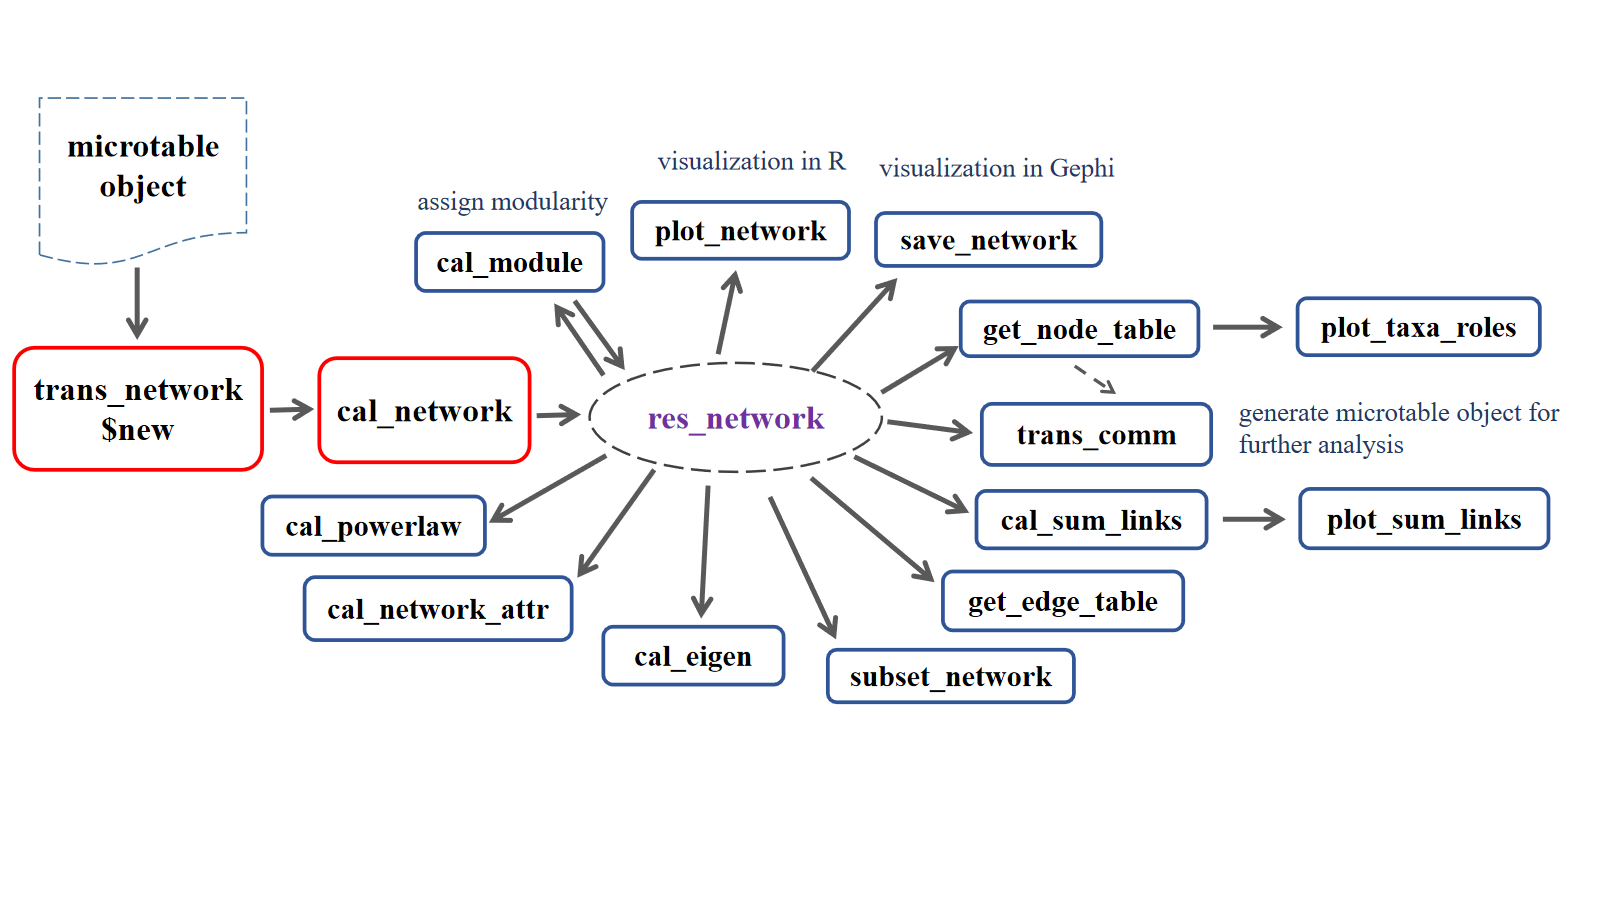
\includegraphics[width=8000px]{Images/network_framework} \end{center}

The objects inside the rectangle with full line represent functions.
The dashed line denotes the key objects (input or output). The \texttt{res\_network} inside the ellipse with dashed line means it is a hub object for other analysis.

\hypertarget{example-5}{%
\subsection{Example}\label{example-5}}

The correlation-based network is selected to show the main operations.
This is only intended to show some operations conveniently.
\textbf{Do not mean we are suggesting this approach in any case}.
Please check the final part for other network construction methods.

\begin{Shaded}
\begin{Highlighting}[]
\CommentTok{\# The parameter cor\_method in trans\_network is used to select correlation calculation method.}
\CommentTok{\# default pearson or spearman correlation invoke R base cor.test, a little slow}
\NormalTok{t1 }\OtherTok{\textless{}{-}}\NormalTok{ trans\_network}\SpecialCharTok{$}\FunctionTok{new}\NormalTok{(}\AttributeTok{dataset =}\NormalTok{ dataset, }\AttributeTok{cor\_method =} \StringTok{"spearman"}\NormalTok{, }\AttributeTok{filter\_thres =} \FloatTok{0.001}\NormalTok{)}
\CommentTok{\# return t1$res\_cor\_p list, containing two tables: correlation coefficient table and p value table}
\end{Highlighting}
\end{Shaded}

Spearman correlation based on WGCNA package is applied to show all the following operations.

\begin{Shaded}
\begin{Highlighting}[]
\CommentTok{\# require WGCNA package}
\ControlFlowTok{if}\NormalTok{(}\SpecialCharTok{!}\FunctionTok{require}\NormalTok{(}\StringTok{"WGCNA"}\NormalTok{)) }\FunctionTok{install.packages}\NormalTok{(}\StringTok{"WGCNA"}\NormalTok{, }\AttributeTok{repos =}\NormalTok{ BiocManager}\SpecialCharTok{::}\FunctionTok{repositories}\NormalTok{())}
\NormalTok{t1 }\OtherTok{\textless{}{-}}\NormalTok{ trans\_network}\SpecialCharTok{$}\FunctionTok{new}\NormalTok{(}\AttributeTok{dataset =}\NormalTok{ dataset, }\AttributeTok{cor\_method =} \StringTok{"spearman"}\NormalTok{, }\AttributeTok{use\_WGCNA\_pearson\_spearman =} \ConstantTok{TRUE}\NormalTok{, }\AttributeTok{filter\_thres =} \FloatTok{0.0001}\NormalTok{)}
\end{Highlighting}
\end{Shaded}

The parameter \texttt{COR\_cut} can be used to select the correlation threshold.
Furthermore, \texttt{COR\_optimization\ =\ TRUE} can be used to find the optimized coefficient threshold (potential transition point of network eigenvalues)
instead of the \texttt{COR\_cut} based on the RMT theory \citep{Deng_Molecular_2012}.

\begin{Shaded}
\begin{Highlighting}[]
\CommentTok{\# construct network; require igraph package}
\NormalTok{t1}\SpecialCharTok{$}\FunctionTok{cal\_network}\NormalTok{(}\AttributeTok{COR\_p\_thres =} \FloatTok{0.01}\NormalTok{, }\AttributeTok{COR\_optimization =} \ConstantTok{TRUE}\NormalTok{)}
\CommentTok{\# use arbitrary coefficient threshold to contruct network}
\NormalTok{t1}\SpecialCharTok{$}\FunctionTok{cal\_network}\NormalTok{(}\AttributeTok{COR\_p\_thres =} \FloatTok{0.01}\NormalTok{, }\AttributeTok{COR\_cut =} \FloatTok{0.7}\NormalTok{)}
\CommentTok{\# return t1$res\_network}
\end{Highlighting}
\end{Shaded}

Then, let's partition modules for the network.

\begin{Shaded}
\begin{Highlighting}[]
\CommentTok{\# invoke igraph cluster\_fast\_greedy function for this undirected network }
\NormalTok{t1}\SpecialCharTok{$}\FunctionTok{cal\_module}\NormalTok{(}\AttributeTok{method =} \StringTok{"cluster\_fast\_greedy"}\NormalTok{)}
\end{Highlighting}
\end{Shaded}

The following operation is to save network to gexf format for the visualization with Gephi(\url{https://gephi.org/}).
The file `network.gexf' can be directly opened by Gephi.

\begin{Shaded}
\begin{Highlighting}[]
\CommentTok{\# require rgexf package to be installed}
\NormalTok{t1}\SpecialCharTok{$}\FunctionTok{save\_network}\NormalTok{(}\AttributeTok{filepath =} \StringTok{"network.gexf"}\NormalTok{)}
\end{Highlighting}
\end{Shaded}

Then, we plot the network in Gephi and present the node colors according to the partitioned modules.

\begin{center}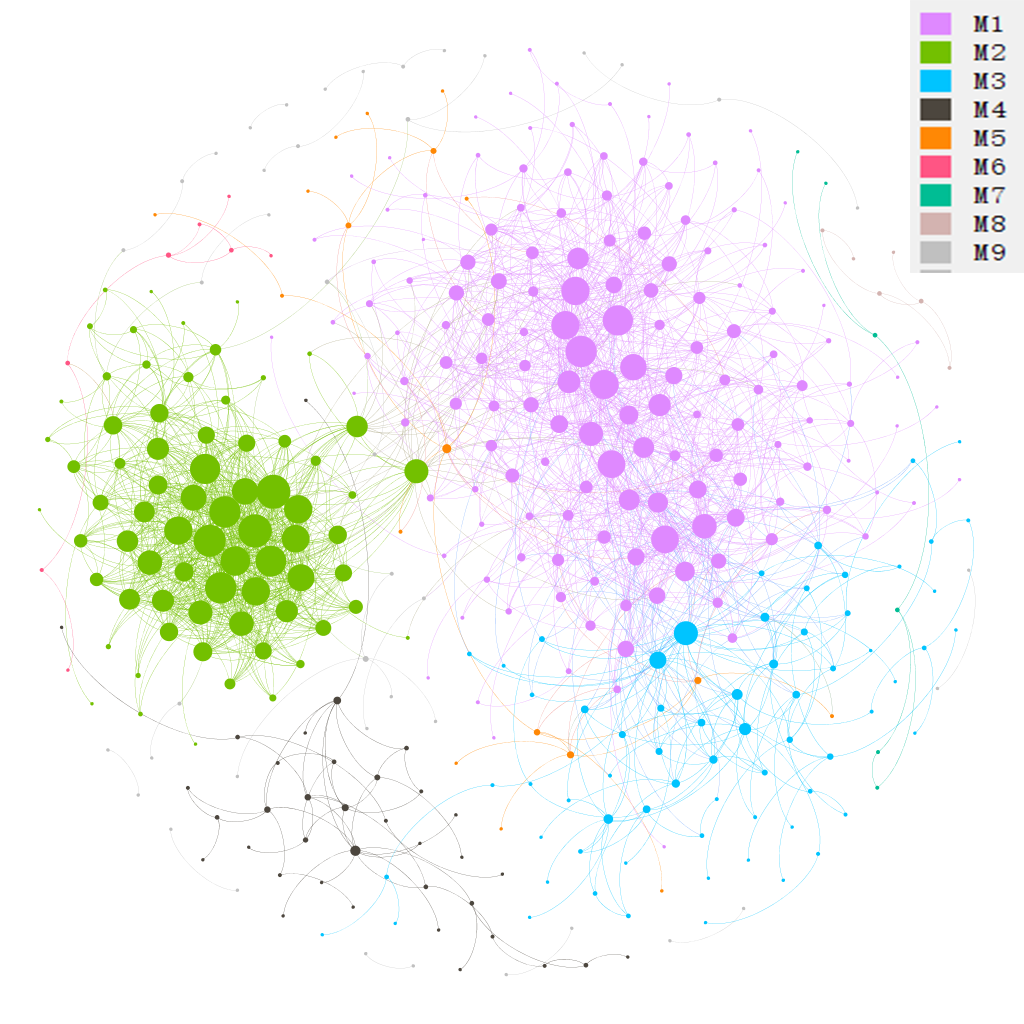
\includegraphics[width=550px]{Images/network1_spearman} \end{center}

Now, we show the node colors with the Phylum information and the edges colors with the positive and negative correlations.
All the data used has been stored in the network.gexf file, including modules classifications, Phylum information and edge labels.

\begin{center}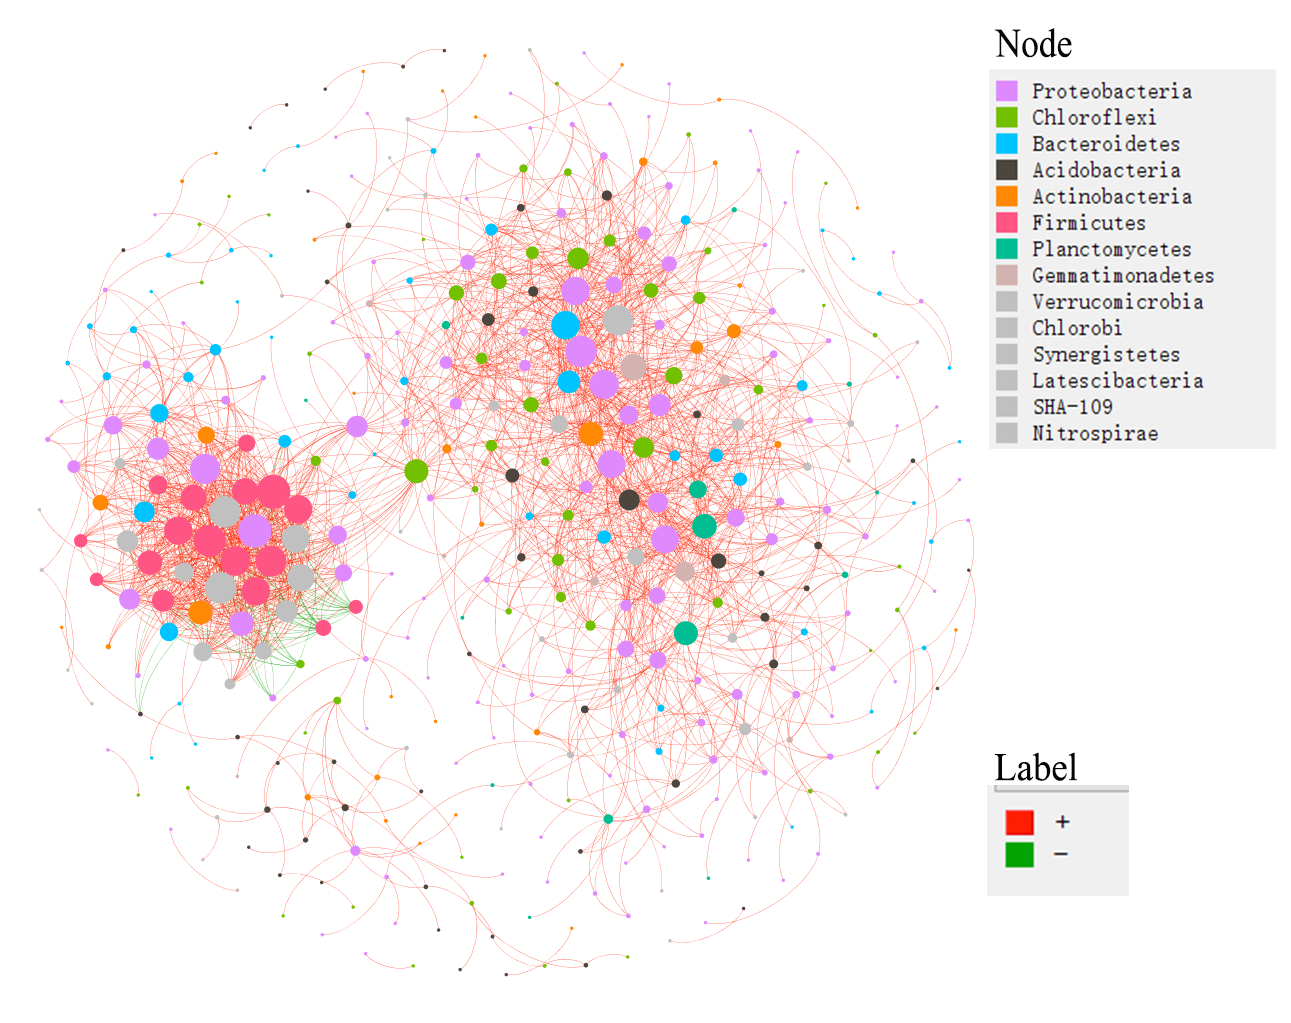
\includegraphics[width=550px]{Images/network2_spearman} \end{center}

\begin{Shaded}
\begin{Highlighting}[]
\CommentTok{\# calculate network attributes}
\NormalTok{t1}\SpecialCharTok{$}\FunctionTok{cal\_network\_attr}\NormalTok{()}
\NormalTok{t1}\SpecialCharTok{$}\NormalTok{res\_network\_attr}
\end{Highlighting}
\end{Shaded}

\begin{longtable}[]{@{}
  >{\centering\arraybackslash}p{(\columnwidth - 2\tabcolsep) * \real{0.3472}}
  >{\centering\arraybackslash}p{(\columnwidth - 2\tabcolsep) * \real{0.1389}}@{}}
\toprule()
\begin{minipage}[b]{\linewidth}\centering
Property
\end{minipage} & \begin{minipage}[b]{\linewidth}\centering
Value
\end{minipage} \\
\midrule()
\endhead
Vertex & 407 \\
Edge & 1989 \\
Average\_degree & 9.774 \\
Average\_path\_length & 3.878 \\
Network\_diameter & 9 \\
Clustering\_coefficient & 0.4698 \\
Density & 0.02407 \\
Heterogeneity & 1.194 \\
Centralization & 0.09908 \\
\bottomrule()
\end{longtable}

The function get\_node\_table, get\_edge\_table and get\_adjacency\_matrix are designed to
get node properties table, edge properties table and adjacency matrix from network, respectively.

\begin{Shaded}
\begin{Highlighting}[]
\CommentTok{\# get node properties}
\NormalTok{t1}\SpecialCharTok{$}\FunctionTok{get\_node\_table}\NormalTok{(}\AttributeTok{node\_roles =} \ConstantTok{TRUE}\NormalTok{)}
\CommentTok{\# return t1$res\_node\_table}
\end{Highlighting}
\end{Shaded}

\begin{longtable}[]{@{}
  >{\centering\arraybackslash}p{(\columnwidth - 12\tabcolsep) * \real{0.1772}}
  >{\centering\arraybackslash}p{(\columnwidth - 12\tabcolsep) * \real{0.1266}}
  >{\centering\arraybackslash}p{(\columnwidth - 12\tabcolsep) * \real{0.1139}}
  >{\centering\arraybackslash}p{(\columnwidth - 12\tabcolsep) * \real{0.1772}}
  >{\centering\arraybackslash}p{(\columnwidth - 12\tabcolsep) * \real{0.1519}}
  >{\centering\arraybackslash}p{(\columnwidth - 12\tabcolsep) * \real{0.1139}}
  >{\centering\arraybackslash}p{(\columnwidth - 12\tabcolsep) * \real{0.1392}}@{}}
\toprule()
\begin{minipage}[b]{\linewidth}\centering
~
\end{minipage} & \begin{minipage}[b]{\linewidth}\centering
name
\end{minipage} & \begin{minipage}[b]{\linewidth}\centering
degree
\end{minipage} & \begin{minipage}[b]{\linewidth}\centering
betweenness
\end{minipage} & \begin{minipage}[b]{\linewidth}\centering
Abundance
\end{minipage} & \begin{minipage}[b]{\linewidth}\centering
module
\end{minipage} & \begin{minipage}[b]{\linewidth}\centering
z
\end{minipage} \\
\midrule()
\endhead
\textbf{OTU\_50} & OTU\_50 & 2 & 0 & 0.2301 & M2 & -1.305 \\
\textbf{OTU\_305} & OTU\_305 & 3 & 4 & 0.1394 & M8 & 1.118 \\
\textbf{OTU\_1} & OTU\_1 & 21 & 2 & 1.409 & M2 & -0.04067 \\
\textbf{OTU\_41} & OTU\_41 & 1 & 0 & 0.1603 & M14 & -0.5774 \\
\textbf{OTU\_59} & OTU\_59 & 3 & 2306 & 0.5588 & M6 & 0.7771 \\
\bottomrule()
\end{longtable}

\begin{Shaded}
\begin{Highlighting}[]
\CommentTok{\# get edge properties}
\NormalTok{t1}\SpecialCharTok{$}\FunctionTok{get\_edge\_table}\NormalTok{()}
\CommentTok{\# return t1$res\_edge\_table }
\NormalTok{t1}\SpecialCharTok{$}\FunctionTok{get\_adjacency\_matrix}\NormalTok{()}
\CommentTok{\# return t1$res\_adjacency\_matrix}
\end{Highlighting}
\end{Shaded}

Then, let's plot the node classification in terms of the within-module connectivity and among-module connectivity.

\begin{Shaded}
\begin{Highlighting}[]
\CommentTok{\# add\_label = TRUE can be used to directly add text label for points}
\NormalTok{t1}\SpecialCharTok{$}\FunctionTok{plot\_taxa\_roles}\NormalTok{(}\AttributeTok{use\_type =} \DecValTok{1}\NormalTok{)}
\end{Highlighting}
\end{Shaded}

\begin{center}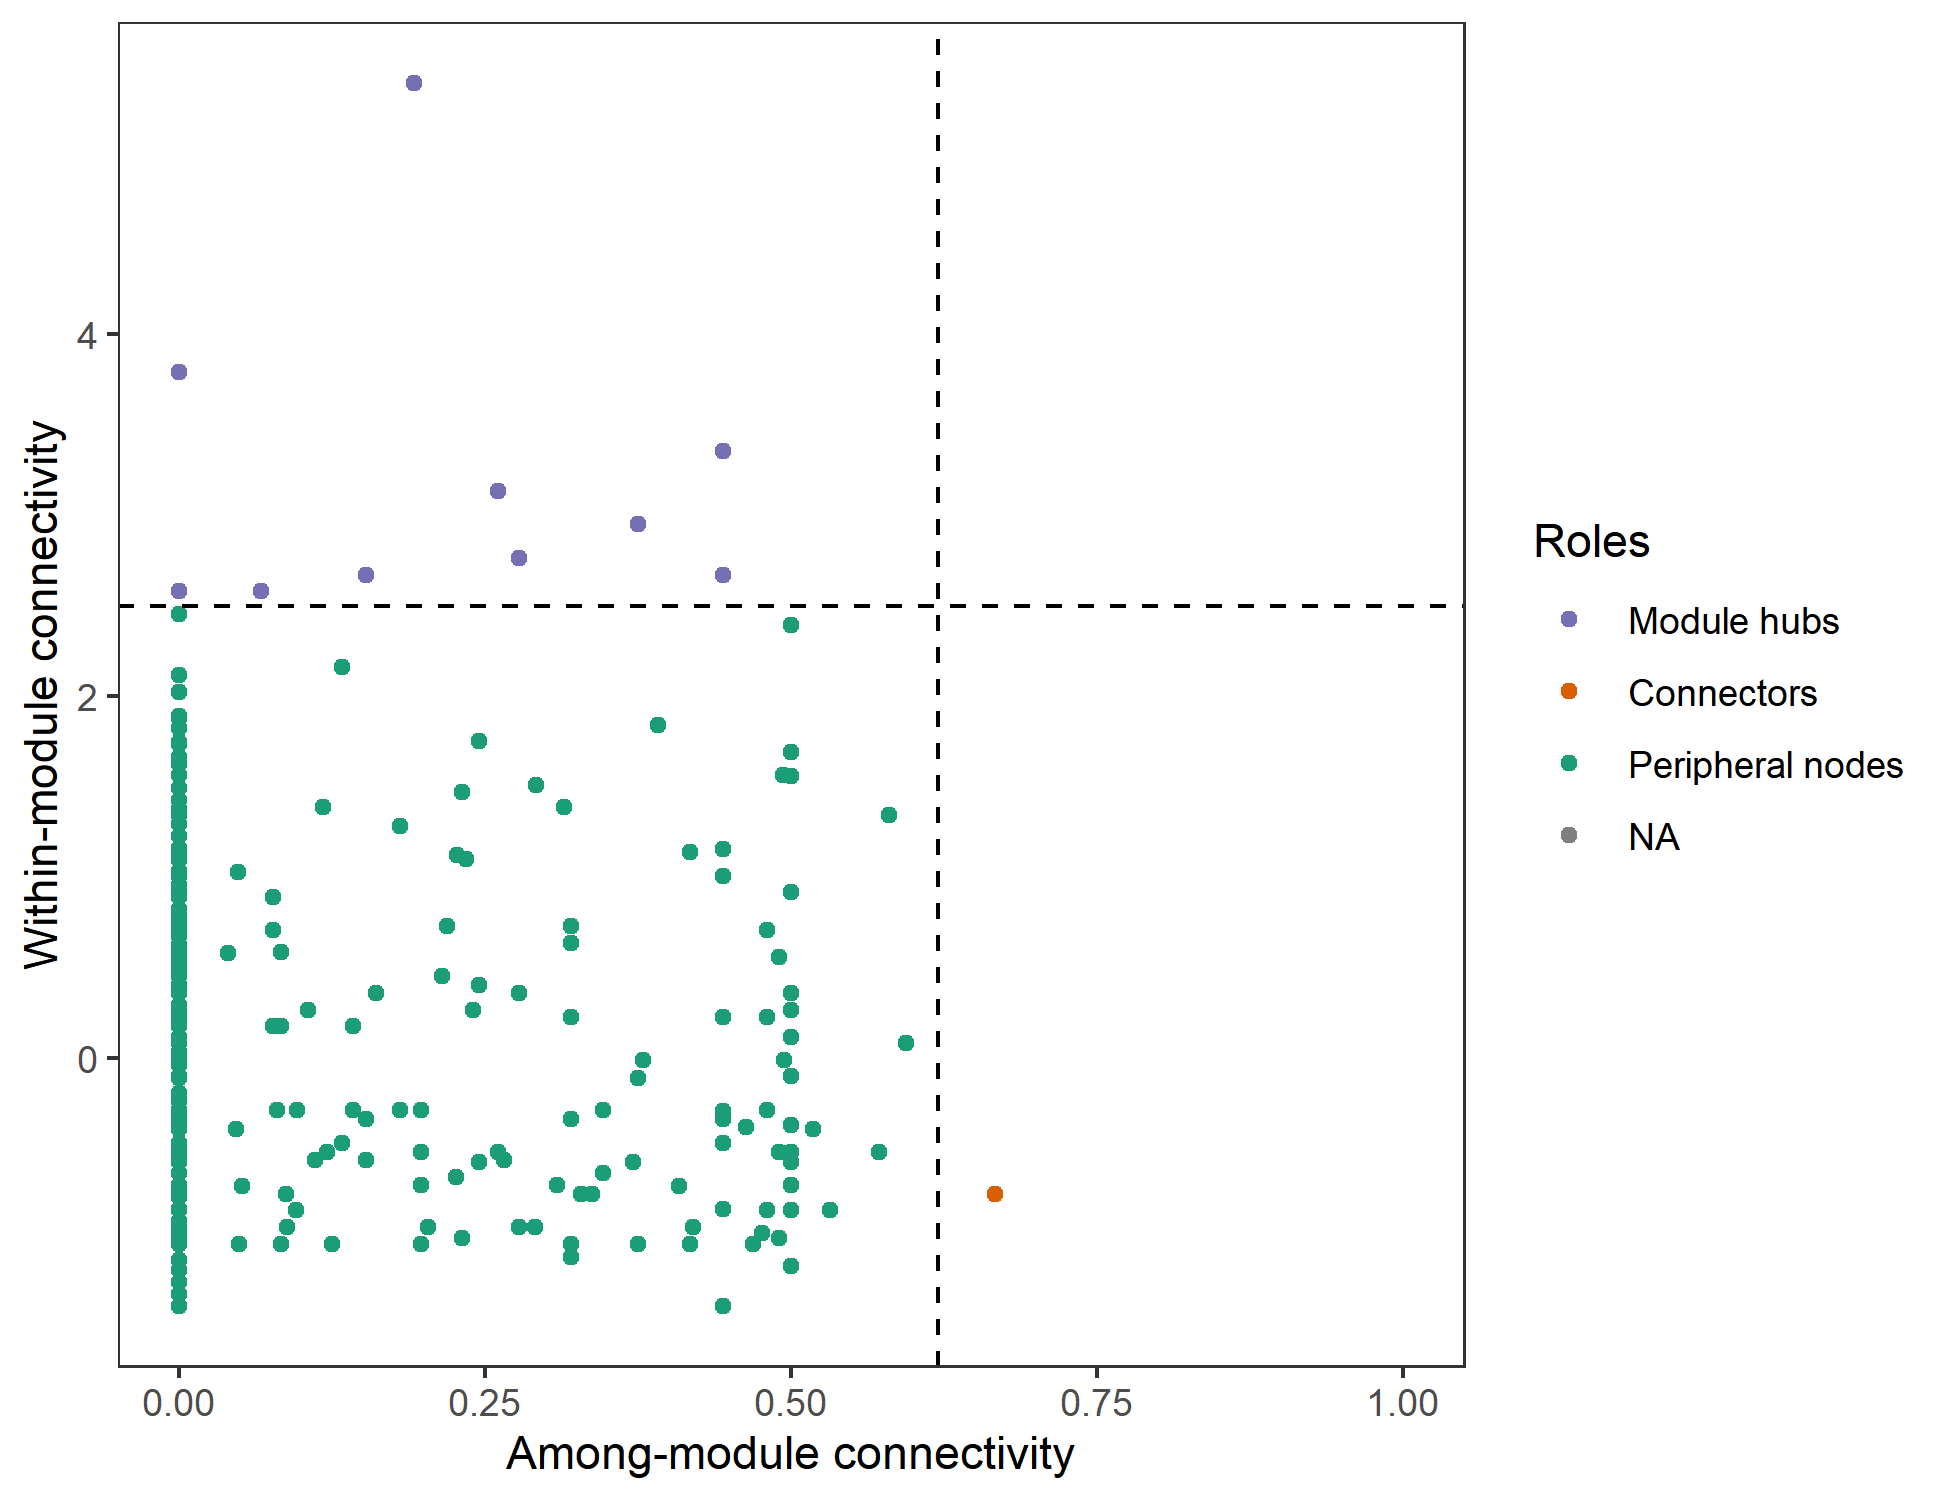
\includegraphics[width=700px]{Images/trans_network_taxa_roles} \end{center}

\begin{Shaded}
\begin{Highlighting}[]
\CommentTok{\# plot node roles with phylum information}
\NormalTok{t1}\SpecialCharTok{$}\FunctionTok{plot\_taxa\_roles}\NormalTok{(}\AttributeTok{use\_type =} \DecValTok{2}\NormalTok{)}
\end{Highlighting}
\end{Shaded}

\begin{center}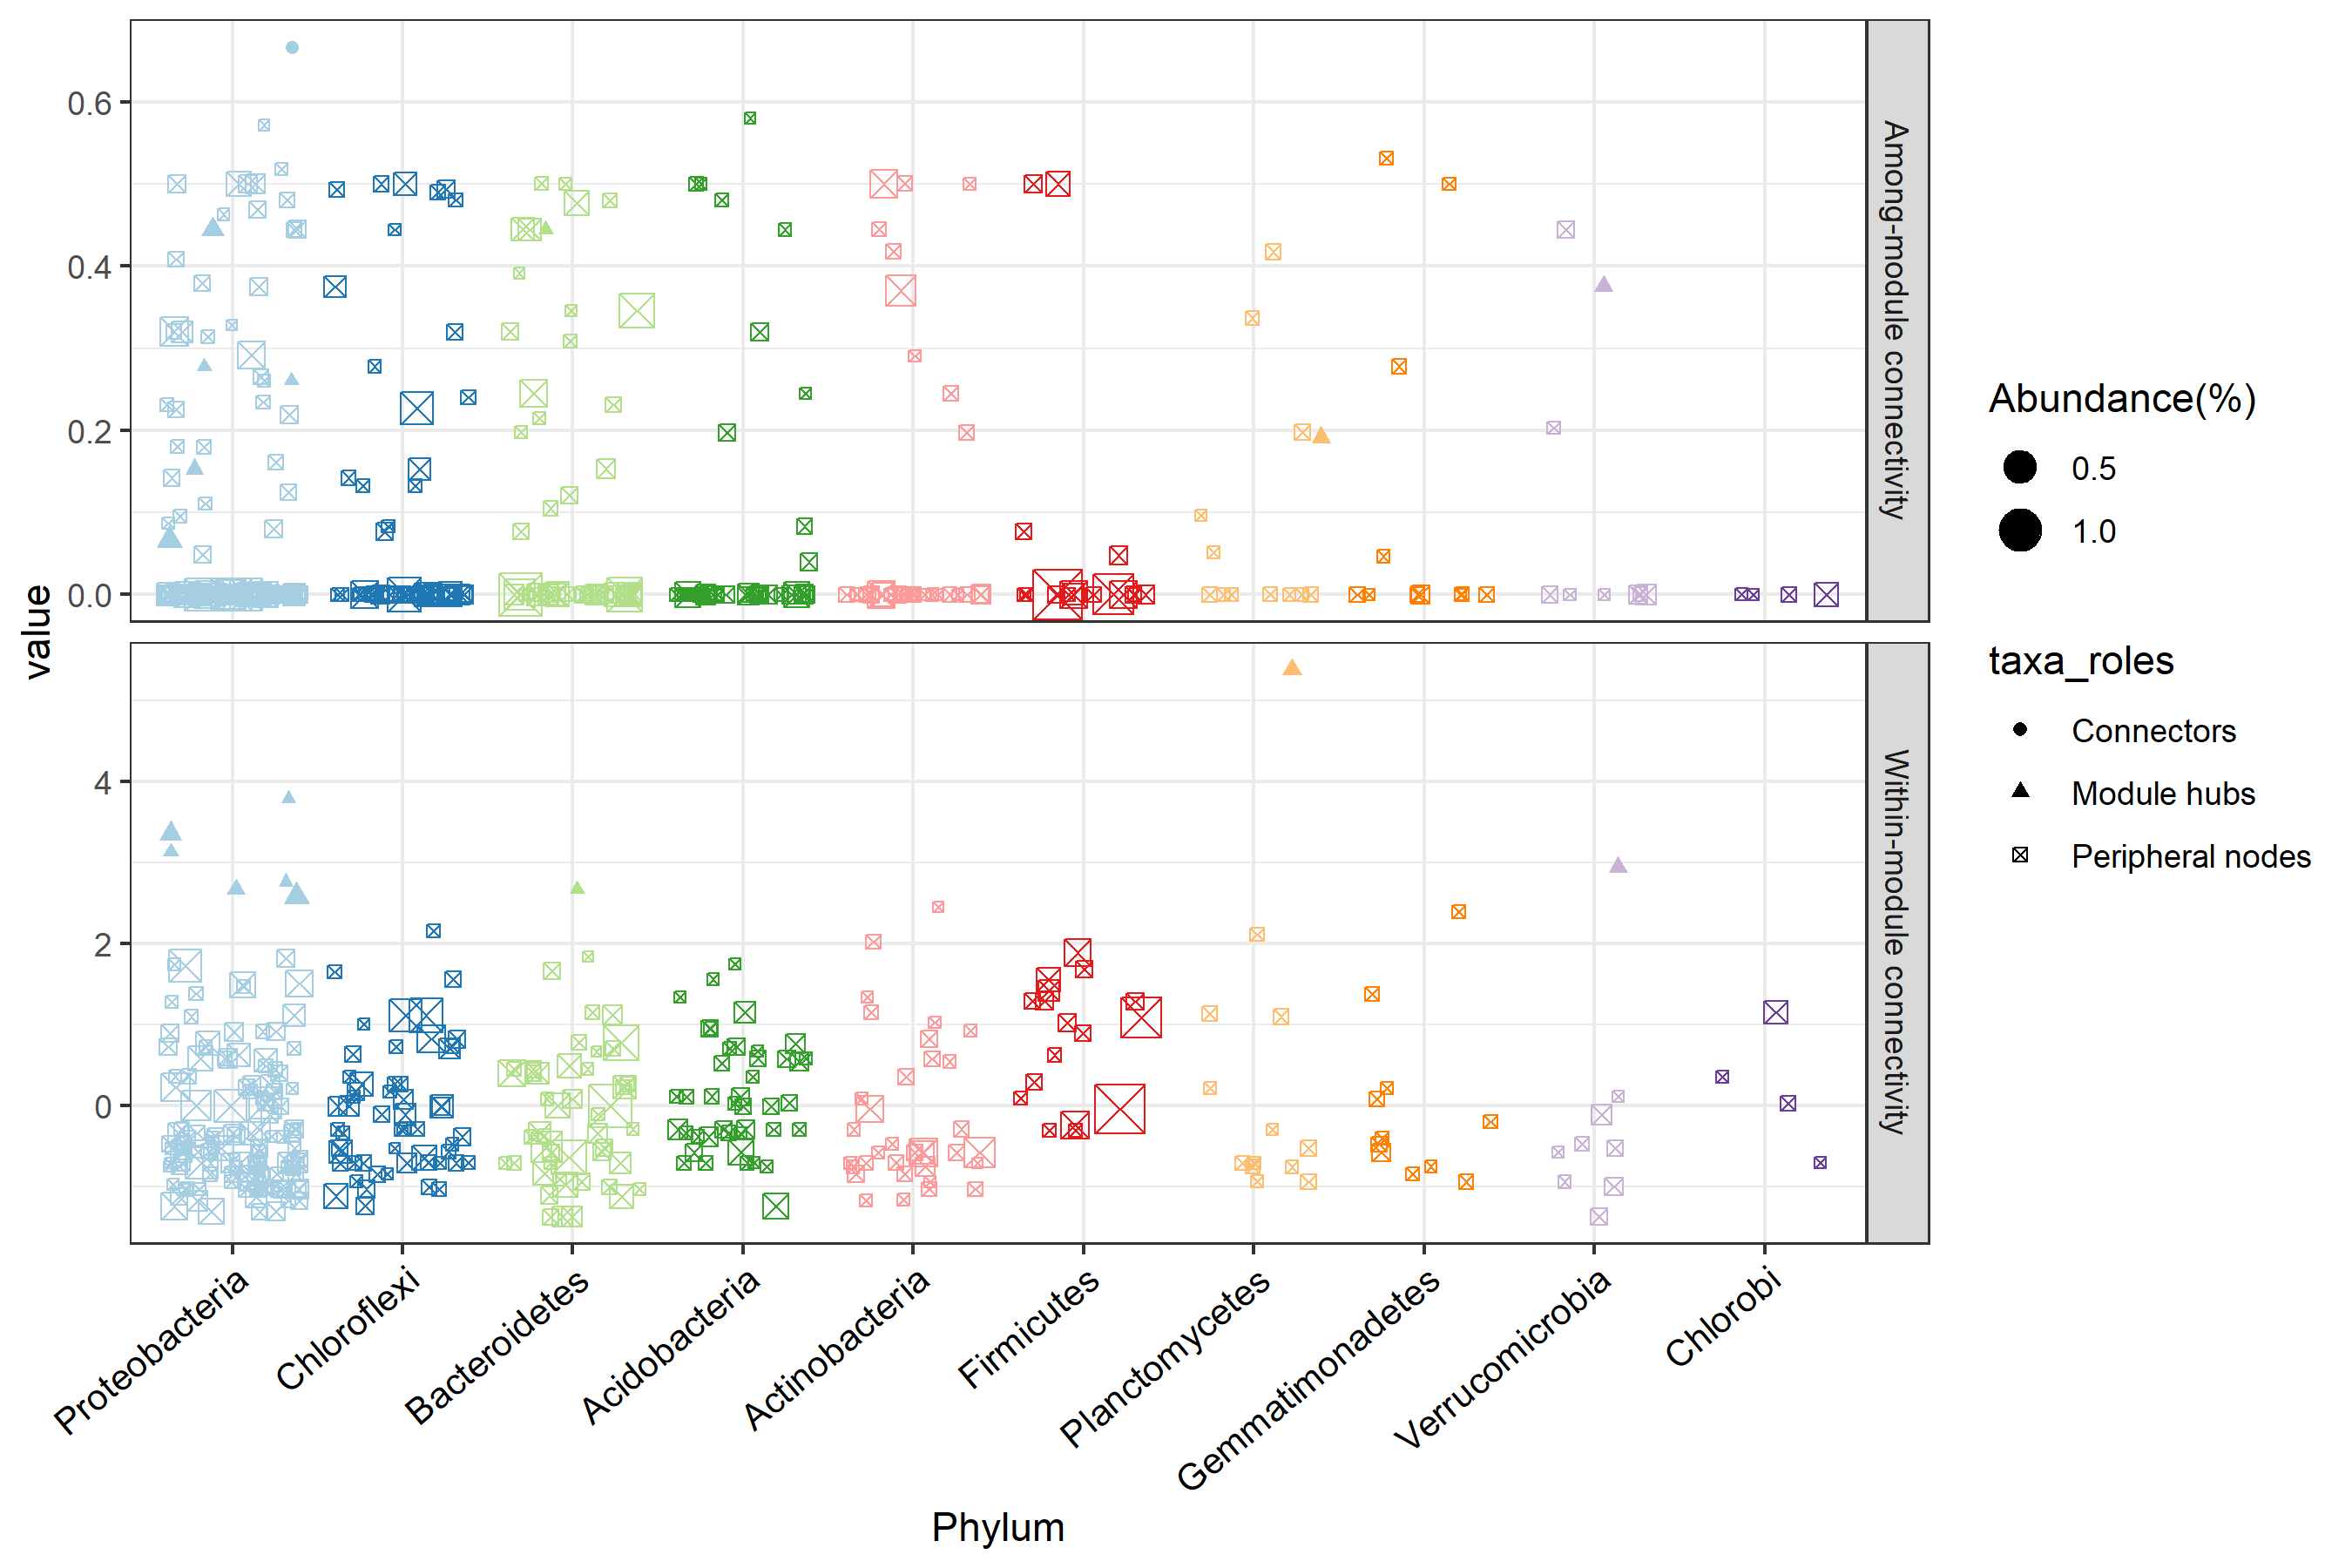
\includegraphics[width=800px]{Images/trans_network_taxa_roles_2} \end{center}

Now, we show the eigengene analysis of modules.
The eigengene of a module, i.e.~the first principal component of PCA, represents the main variance of the abundance in the species of the module.

\begin{Shaded}
\begin{Highlighting}[]
\NormalTok{t1}\SpecialCharTok{$}\FunctionTok{cal\_eigen}\NormalTok{()}
\CommentTok{\# return t1$res\_eigen}
\end{Highlighting}
\end{Shaded}

Then we perform correlation heatmap to show the associations between eigengenes and environmental factors.

\begin{Shaded}
\begin{Highlighting}[]
\CommentTok{\# create trans\_env object}
\NormalTok{t2 }\OtherTok{\textless{}{-}}\NormalTok{ trans\_env}\SpecialCharTok{$}\FunctionTok{new}\NormalTok{(}\AttributeTok{dataset =}\NormalTok{ dataset, }\AttributeTok{add\_data =}\NormalTok{ env\_data\_16S[, }\DecValTok{4}\SpecialCharTok{:}\DecValTok{11}\NormalTok{])}
\CommentTok{\# calculate correlations}
\NormalTok{t2}\SpecialCharTok{$}\FunctionTok{cal\_cor}\NormalTok{(}\AttributeTok{add\_abund\_table =}\NormalTok{ t1}\SpecialCharTok{$}\NormalTok{res\_eigen)}
\CommentTok{\# plot the correlation heatmap}
\NormalTok{t2}\SpecialCharTok{$}\FunctionTok{plot\_cor}\NormalTok{()}
\end{Highlighting}
\end{Shaded}

\begin{center}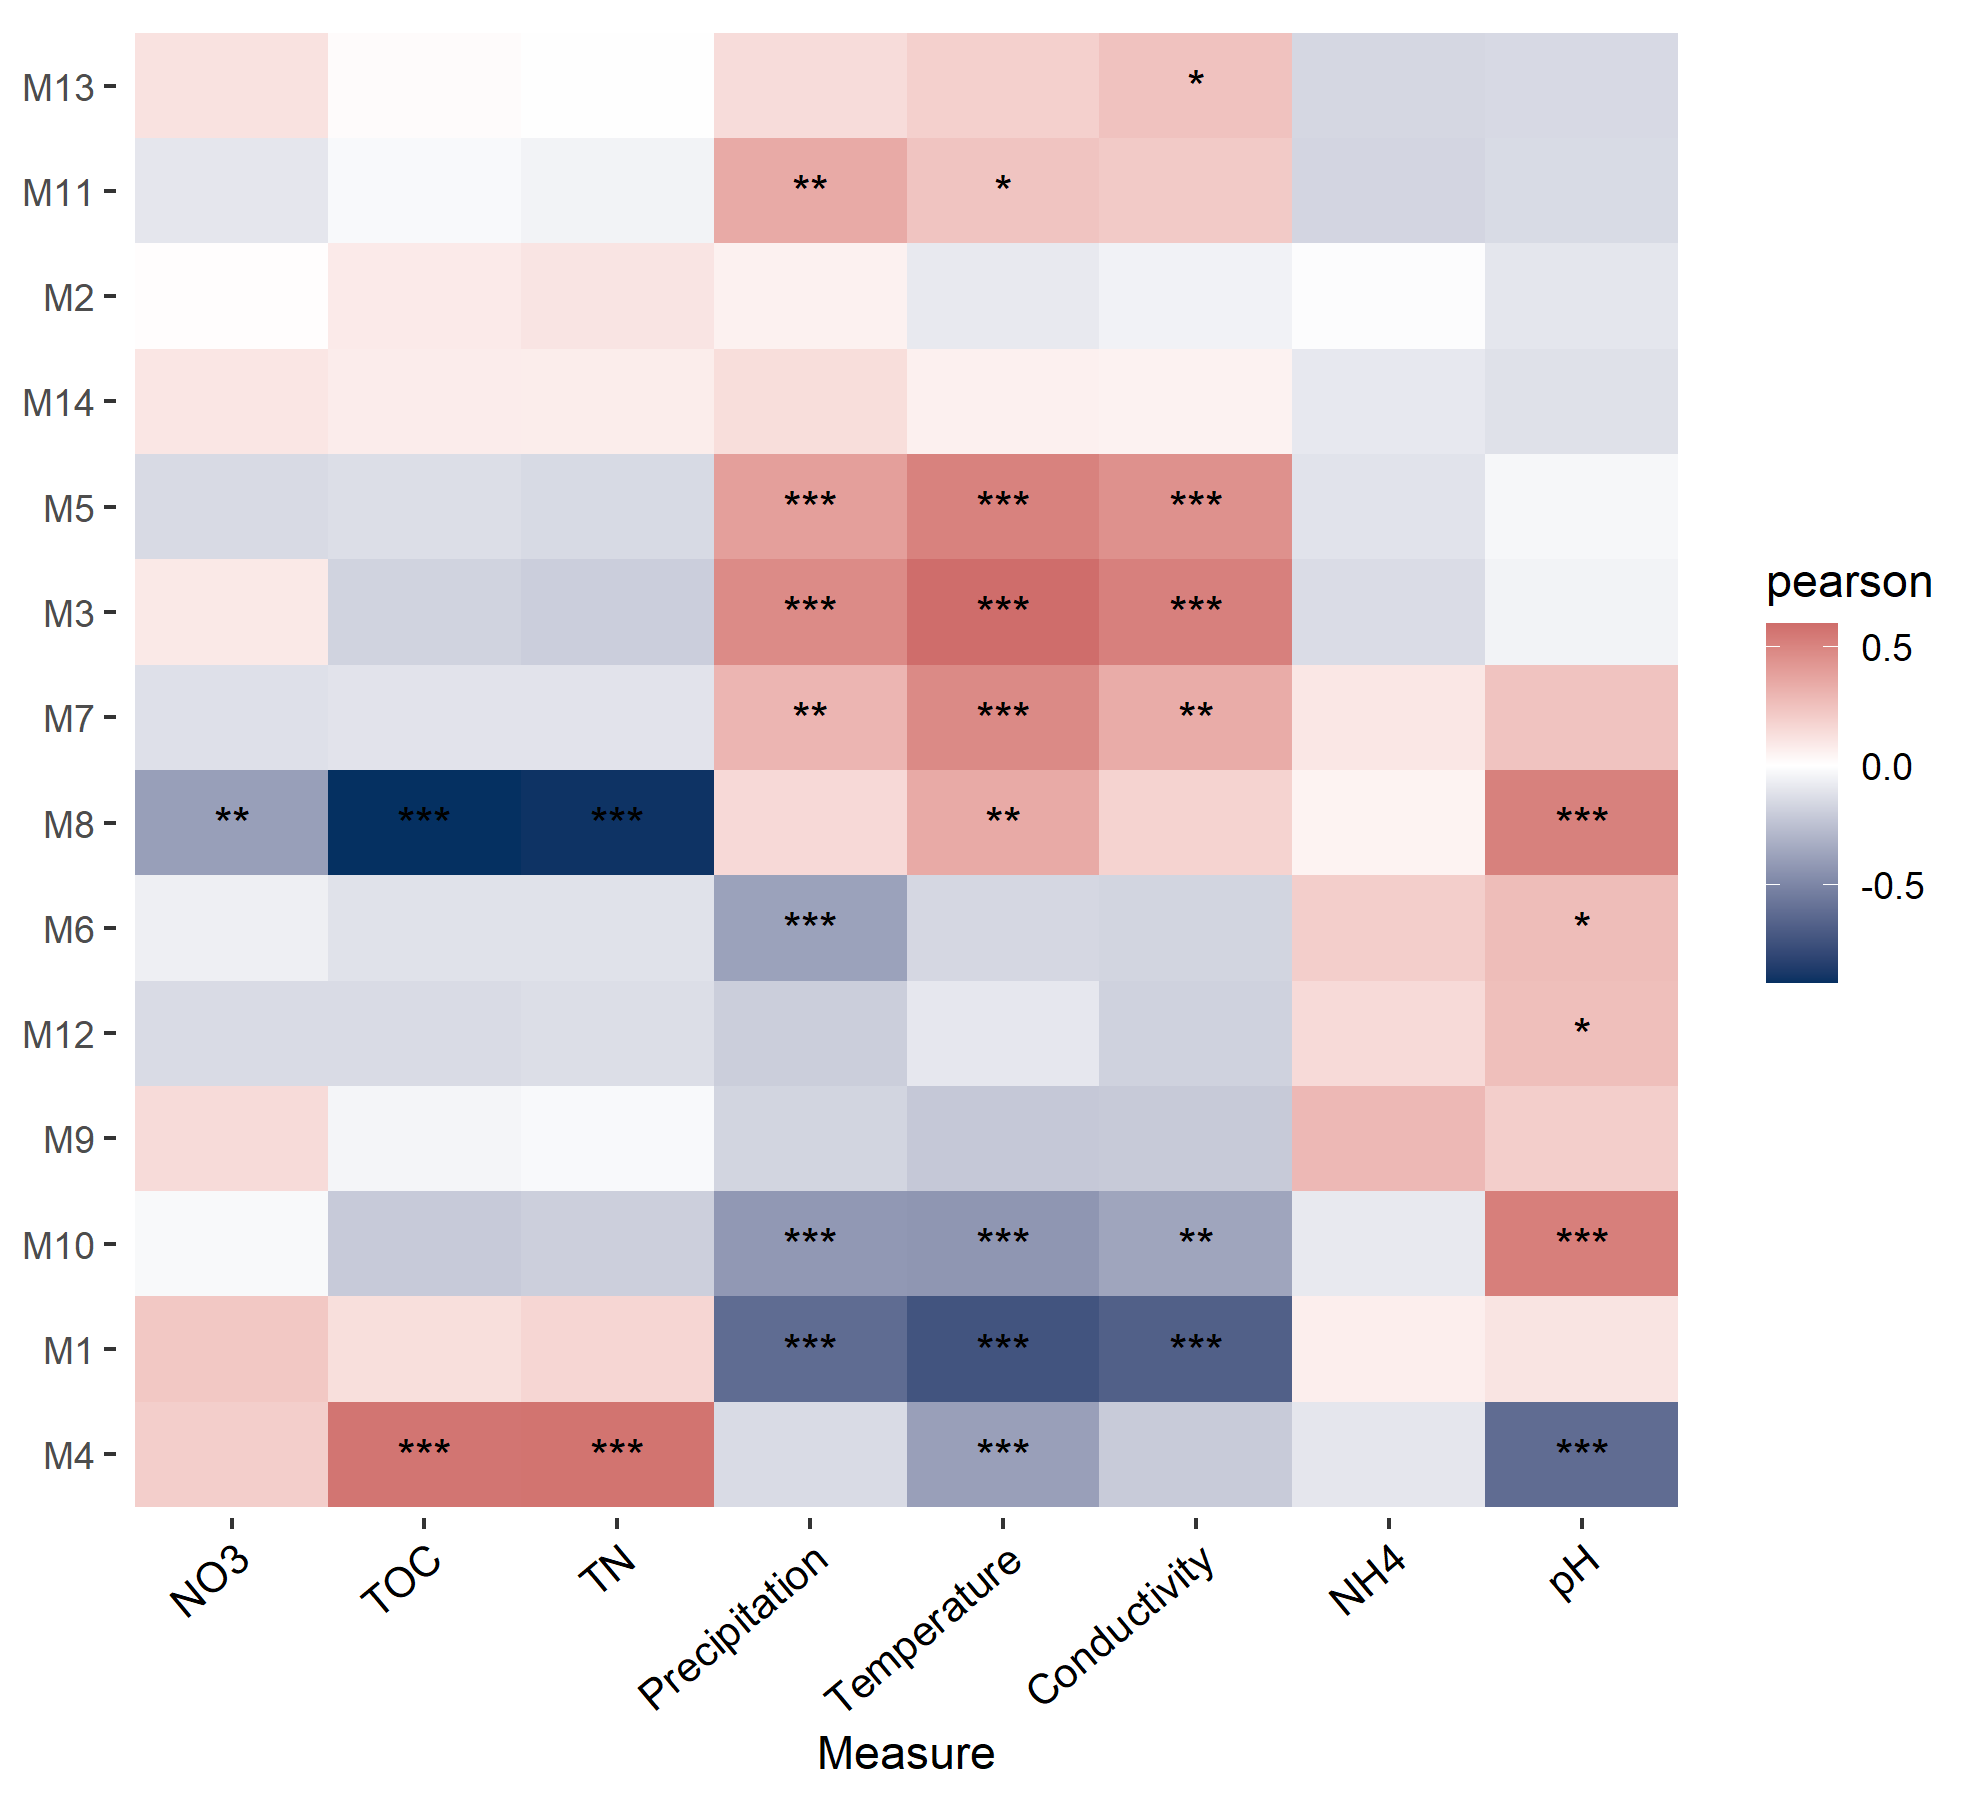
\includegraphics[width=600px]{Images/trans_network_env_module_eigen} \end{center}

The \texttt{subset\_network} function can be applied to extract a part of nodes and edges among these nodes from the network.
In this function, you should provide the nodes you need using the node parameter.

\begin{Shaded}
\begin{Highlighting}[]
\CommentTok{\# extract a sub network that contains all nodes in module M1}
\NormalTok{t1}\SpecialCharTok{$}\FunctionTok{subset\_network}\NormalTok{(}\AttributeTok{node =}\NormalTok{ t1}\SpecialCharTok{$}\NormalTok{res\_node\_table }\SpecialCharTok{\%\textgreater{}\%}\NormalTok{ base}\SpecialCharTok{::}\FunctionTok{subset}\NormalTok{(module }\SpecialCharTok{==} \StringTok{"M1"}\NormalTok{) }\SpecialCharTok{\%\textgreater{}\%}\NormalTok{ rownames, }\AttributeTok{rm\_single =} \ConstantTok{TRUE}\NormalTok{)}
\CommentTok{\# return a new network with igraph class}
\CommentTok{\# extract sub network in which all edge labels are "+", i.e. positive edges}
\NormalTok{t1}\SpecialCharTok{$}\FunctionTok{subset\_network}\NormalTok{(}\AttributeTok{edge =} \StringTok{"+"}\NormalTok{)}
\end{Highlighting}
\end{Shaded}

Then let's show how to extract sub-network for samples \citep{Ma_Geographic_2016}.

\begin{Shaded}
\begin{Highlighting}[]
\CommentTok{\# extract the sub{-}network of sample \textquotesingle{}S1\textquotesingle{}}
\NormalTok{sub1 }\OtherTok{\textless{}{-}}\NormalTok{ t1}\SpecialCharTok{$}\FunctionTok{subset\_network}\NormalTok{(}\AttributeTok{node =}\NormalTok{ dataset}\SpecialCharTok{$}\NormalTok{otu\_table }\SpecialCharTok{\%\textgreater{}\%}\NormalTok{ .[.[, }\StringTok{"S1"}\NormalTok{] }\SpecialCharTok{!=} \DecValTok{0}\NormalTok{, ] }\SpecialCharTok{\%\textgreater{}\%}\NormalTok{ rownames, }\AttributeTok{rm\_single =} \ConstantTok{TRUE}\NormalTok{)}
\CommentTok{\# see https://chiliubio.github.io/microeco\_tutorial/notes.html\#clone for the \textquotesingle{}clone\textquotesingle{} function explanation}
\NormalTok{t2 }\OtherTok{\textless{}{-}} \FunctionTok{clone}\NormalTok{(t1)}
\NormalTok{t2}\SpecialCharTok{$}\NormalTok{res\_network }\OtherTok{\textless{}{-}}\NormalTok{ sub1}
\CommentTok{\# then t2 have a network for \textquotesingle{}S1\textquotesingle{} and can be used for further analysis}
\NormalTok{t2}\SpecialCharTok{$}\FunctionTok{cal\_module}\NormalTok{()}
\NormalTok{t2}\SpecialCharTok{$}\FunctionTok{save\_network}\NormalTok{(}\StringTok{"S1.gexf"}\NormalTok{)}
\CommentTok{\# please use a loop for all samples}
\end{Highlighting}
\end{Shaded}

We also add the function \texttt{plot\_network} to directly plot the network in R, including the static network and dynamic network.
The static network is suitable for the case with relatively few nodes, while dynamic network can be better applied to a large network.
See \url{https://yunranchen.github.io/intro-net-r/advanced-network-visualization.html} and \url{https://kateto.net/network-visualization} for more
details on the network visualization in R.

\begin{Shaded}
\begin{Highlighting}[]
\CommentTok{\# default parameter represents using igraph plot.igraph function}
\NormalTok{t2}\SpecialCharTok{$}\FunctionTok{plot\_network}\NormalTok{()}
\CommentTok{\# use ggraph method; require ggraph package}
\CommentTok{\# If ggraph is not installed; first install it with command: install.packages("ggraph")}
\NormalTok{t2}\SpecialCharTok{$}\FunctionTok{plot\_network}\NormalTok{(}\AttributeTok{method =} \StringTok{"ggraph"}\NormalTok{, }\AttributeTok{node\_color =} \StringTok{"Phylum"}\NormalTok{)}
\CommentTok{\# use networkD3 package method for the dynamic network visualization in R}
\CommentTok{\# If networkD3 is not installed; first install it with command: install.packages("networkD3")}
\NormalTok{t1}\SpecialCharTok{$}\FunctionTok{plot\_network}\NormalTok{(}\AttributeTok{method =} \StringTok{"networkD3"}\NormalTok{, }\AttributeTok{node\_color =} \StringTok{"module"}\NormalTok{)}
\NormalTok{t1}\SpecialCharTok{$}\FunctionTok{plot\_network}\NormalTok{(}\AttributeTok{method =} \StringTok{"networkD3"}\NormalTok{, }\AttributeTok{node\_color =} \StringTok{"Phylum"}\NormalTok{)}
\end{Highlighting}
\end{Shaded}

The \texttt{trans\_comm} function can be used to convert the node classification to a new microtable object for other analysis.

\begin{Shaded}
\begin{Highlighting}[]
\CommentTok{\# use\_col is used to select a column of t1$res\_node\_table}
\NormalTok{tmp }\OtherTok{\textless{}{-}}\NormalTok{ t1}\SpecialCharTok{$}\FunctionTok{trans\_comm}\NormalTok{(}\AttributeTok{use\_col =} \StringTok{"module"}\NormalTok{, }\AttributeTok{abundance =} \ConstantTok{FALSE}\NormalTok{)}
\NormalTok{tmp}
\NormalTok{tmp}\SpecialCharTok{$}\NormalTok{otu\_table[tmp}\SpecialCharTok{$}\NormalTok{otu\_table }\SpecialCharTok{\textgreater{}} \DecValTok{0}\NormalTok{] }\OtherTok{\textless{}{-}} \DecValTok{1}
\NormalTok{tmp}\SpecialCharTok{$}\FunctionTok{tidy\_dataset}\NormalTok{()}
\NormalTok{tmp}\SpecialCharTok{$}\FunctionTok{cal\_abund}\NormalTok{()}
\NormalTok{tmp2 }\OtherTok{\textless{}{-}}\NormalTok{ trans\_abund}\SpecialCharTok{$}\FunctionTok{new}\NormalTok{(tmp, }\AttributeTok{taxrank =} \StringTok{"Phylum"}\NormalTok{, }\AttributeTok{ntaxa =} \DecValTok{10}\NormalTok{)}
\NormalTok{tmp2}\SpecialCharTok{$}\NormalTok{data\_abund}\SpecialCharTok{$}\NormalTok{Sample }\SpecialCharTok{\%\textless{}\textgreater{}\%} \FunctionTok{factor}\NormalTok{(., }\AttributeTok{levels =} \FunctionTok{rownames}\NormalTok{(tmp}\SpecialCharTok{$}\NormalTok{sample\_table))}
\NormalTok{tmp2}\SpecialCharTok{$}\FunctionTok{plot\_line}\NormalTok{(}\AttributeTok{xtext\_angle =} \DecValTok{30}\NormalTok{, }\AttributeTok{color\_values =}\NormalTok{ RColorBrewer}\SpecialCharTok{::}\FunctionTok{brewer.pal}\NormalTok{(}\DecValTok{12}\NormalTok{, }\StringTok{"Paired"}\NormalTok{)) }\SpecialCharTok{+} \FunctionTok{ylab}\NormalTok{(}\StringTok{"OTUs ratio (\%)"}\NormalTok{)}
\end{Highlighting}
\end{Shaded}

The function \texttt{cal\_sum\_links} can sum the links (edge) number from one taxa to another or within the same taxa.
The function \texttt{plot\_sum\_links} is used to show the result from the function \texttt{cal\_sum\_links}.
This is very useful to fast see how many nodes are connected between different taxa or within one taxa.
In terms of `Phylum' level in the tutorial, the function cal\_sum\_links() sum the linkages number from one Phylum to another Phylum or the linkages in the same Phylum.
So the numbers along the outside of the circular plot represent how many edges or linkages are related with the Phylum.
For example, in terms of Proteobacteria, there are roughly total 900 edges associated with the OTUs in Proteobacteria,
in which roughly 200 edges connect both OTUs in Proteobacteria and roughly 150 edges connect the OTUs from Proteobacteria with the OTUs from Chloroflexi.

\begin{Shaded}
\begin{Highlighting}[]
\NormalTok{t1}\SpecialCharTok{$}\FunctionTok{cal\_sum\_links}\NormalTok{(}\AttributeTok{taxa\_level =} \StringTok{"Phylum"}\NormalTok{)}
\CommentTok{\# interactive visualization; require chorddiag package; see https://github.com/mattflor/chorddiag}
\NormalTok{t1}\SpecialCharTok{$}\FunctionTok{plot\_sum\_links}\NormalTok{(}\AttributeTok{plot\_pos =} \ConstantTok{TRUE}\NormalTok{, }\AttributeTok{plot\_num =} \DecValTok{10}\NormalTok{, }\AttributeTok{color\_values =}\NormalTok{ RColorBrewer}\SpecialCharTok{::}\FunctionTok{brewer.pal}\NormalTok{(}\DecValTok{10}\NormalTok{, }\StringTok{"Paired"}\NormalTok{))}
\CommentTok{\# From v1.2.0, method = "circlize" is available for conveniently saving the static plot}
\ControlFlowTok{if}\NormalTok{(}\SpecialCharTok{!}\FunctionTok{require}\NormalTok{(}\StringTok{"circlize"}\NormalTok{)) }\FunctionTok{install.packages}\NormalTok{(}\StringTok{"circlize"}\NormalTok{)}
\NormalTok{t1}\SpecialCharTok{$}\FunctionTok{plot\_sum\_links}\NormalTok{(}\AttributeTok{method =} \StringTok{"circlize"}\NormalTok{, }\AttributeTok{transparency =} \FloatTok{0.2}\NormalTok{, }\AttributeTok{annotationTrackHeight =}\NormalTok{ circlize}\SpecialCharTok{::}\FunctionTok{mm\_h}\NormalTok{(}\FunctionTok{c}\NormalTok{(}\DecValTok{5}\NormalTok{, }\DecValTok{5}\NormalTok{)))}
\end{Highlighting}
\end{Shaded}

\begin{center}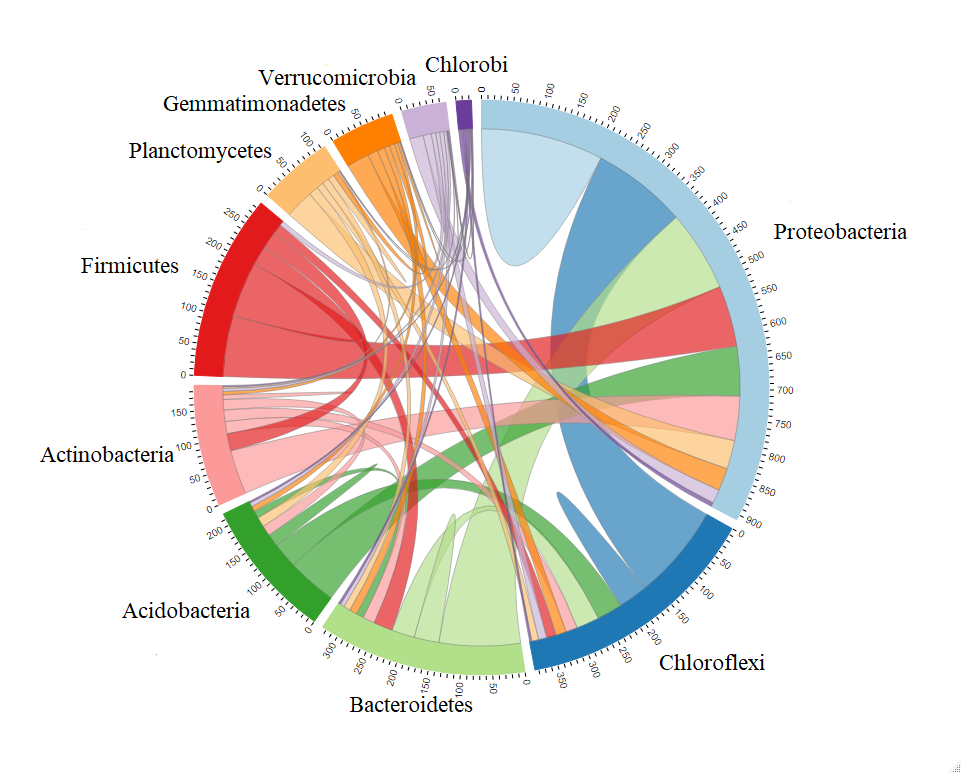
\includegraphics[width=700px]{Images/trans_network_sum_links} \end{center}

For the correlation network, there are also other available correlation/association calculation options,
such as Bray--Curtis (1-dissimilarity), SparCC \citep{Friedman_Inferring_2012}, CCLasso \citep{Fang_CCLasso_2015},
Pearson or Spearman with data normalization based on NetCoMi package \citep{Peschel_NetCoMi_2021}.

\begin{Shaded}
\begin{Highlighting}[]
\CommentTok{\# use Bray–Curtis index (1{-}dissimilarity)}
\NormalTok{t1 }\OtherTok{\textless{}{-}}\NormalTok{ trans\_network}\SpecialCharTok{$}\FunctionTok{new}\NormalTok{(}\AttributeTok{dataset =}\NormalTok{ dataset, }\AttributeTok{cor\_method =} \StringTok{"bray"}\NormalTok{, }\AttributeTok{filter\_thres =} \FloatTok{0.001}\NormalTok{)}
\CommentTok{\# Pearson correlation}
\NormalTok{t1 }\OtherTok{\textless{}{-}}\NormalTok{ trans\_network}\SpecialCharTok{$}\FunctionTok{new}\NormalTok{(}\AttributeTok{dataset =}\NormalTok{ dataset, }\AttributeTok{cor\_method =} \StringTok{"pearson"}\NormalTok{, }\AttributeTok{filter\_thres =} \FloatTok{0.001}\NormalTok{)}
\CommentTok{\# Pearson correlation using WGCNA package}
\CommentTok{\# install WGCNA package}
\ControlFlowTok{if}\NormalTok{(}\SpecialCharTok{!}\FunctionTok{require}\NormalTok{(}\StringTok{"WGCNA"}\NormalTok{)) }\FunctionTok{install.packages}\NormalTok{(}\StringTok{"WGCNA"}\NormalTok{, }\AttributeTok{repos =}\NormalTok{ BiocManager}\SpecialCharTok{::}\FunctionTok{repositories}\NormalTok{())}
\NormalTok{t1 }\OtherTok{\textless{}{-}}\NormalTok{ trans\_network}\SpecialCharTok{$}\FunctionTok{new}\NormalTok{(}\AttributeTok{dataset =}\NormalTok{ dataset, }\AttributeTok{cor\_method =} \StringTok{"pearson"}\NormalTok{, }\AttributeTok{use\_WGCNA\_pearson\_spearman =} \ConstantTok{TRUE}\NormalTok{, }\AttributeTok{filter\_thres =} \FloatTok{0.001}\NormalTok{)}
\CommentTok{\# Pearson correlation using NetCoMi package; install it from https://github.com/stefpeschel/NetCoMi}
\NormalTok{t1 }\OtherTok{\textless{}{-}}\NormalTok{ trans\_network}\SpecialCharTok{$}\FunctionTok{new}\NormalTok{(}\AttributeTok{dataset =}\NormalTok{ dataset, }\AttributeTok{cor\_method =} \StringTok{"pearson"}\NormalTok{, }\AttributeTok{use\_NetCoMi\_pearson\_spearman =} \ConstantTok{TRUE}\NormalTok{, }\AttributeTok{filter\_thres =} \FloatTok{0.001}\NormalTok{)}
\CommentTok{\# Spearman correlation using WGCNA package}
\NormalTok{t1 }\OtherTok{\textless{}{-}}\NormalTok{ trans\_network}\SpecialCharTok{$}\FunctionTok{new}\NormalTok{(}\AttributeTok{dataset =}\NormalTok{ dataset, }\AttributeTok{cor\_method =} \StringTok{"spearman"}\NormalTok{, }\AttributeTok{use\_WGCNA\_pearson\_spearman =} \ConstantTok{TRUE}\NormalTok{, }\AttributeTok{filter\_thres =} \FloatTok{0.001}\NormalTok{)}
\CommentTok{\# Spearman correlation using NetCoMi package}
\NormalTok{t1 }\OtherTok{\textless{}{-}}\NormalTok{ trans\_network}\SpecialCharTok{$}\FunctionTok{new}\NormalTok{(}\AttributeTok{dataset =}\NormalTok{ dataset, }\AttributeTok{cor\_method =} \StringTok{"spearman"}\NormalTok{, }\AttributeTok{use\_NetCoMi\_pearson\_spearman =} \ConstantTok{TRUE}\NormalTok{, }\AttributeTok{filter\_thres =} \FloatTok{0.001}\NormalTok{)}
\CommentTok{\# SparCC method, from SpiecEasi package, see https://github.com/zdk123/SpiecEasi for the installation}
\NormalTok{t1 }\OtherTok{\textless{}{-}}\NormalTok{ trans\_network}\SpecialCharTok{$}\FunctionTok{new}\NormalTok{(}\AttributeTok{dataset =}\NormalTok{ dataset, }\AttributeTok{cor\_method =} \StringTok{"sparcc"}\NormalTok{, }\AttributeTok{use\_sparcc\_method =} \StringTok{"SpiecEasi"}\NormalTok{, }\AttributeTok{filter\_thres =} \FloatTok{0.003}\NormalTok{)}
\CommentTok{\# SparCC method, from NetCoMi package; https://github.com/stefpeschel/NetCoMi}
\NormalTok{t1 }\OtherTok{\textless{}{-}}\NormalTok{ trans\_network}\SpecialCharTok{$}\FunctionTok{new}\NormalTok{(}\AttributeTok{dataset =}\NormalTok{ dataset, }\AttributeTok{cor\_method =} \StringTok{"sparcc"}\NormalTok{, }\AttributeTok{use\_sparcc\_method =} \StringTok{"NetCoMi"}\NormalTok{, }\AttributeTok{filter\_thres =} \FloatTok{0.001}\NormalTok{)}
\CommentTok{\# CCLasso method based on NetCoMi package}
\NormalTok{t1 }\OtherTok{\textless{}{-}}\NormalTok{ trans\_network}\SpecialCharTok{$}\FunctionTok{new}\NormalTok{(}\AttributeTok{dataset =}\NormalTok{ dataset, }\AttributeTok{cor\_method =} \StringTok{"cclasso"}\NormalTok{, }\AttributeTok{filter\_thres =} \FloatTok{0.001}\NormalTok{)}
\CommentTok{\# CCREPE method based on NetCoMi package}
\NormalTok{t1 }\OtherTok{\textless{}{-}}\NormalTok{ trans\_network}\SpecialCharTok{$}\FunctionTok{new}\NormalTok{(}\AttributeTok{dataset =}\NormalTok{ dataset, }\AttributeTok{cor\_method =} \StringTok{"ccrepe"}\NormalTok{, }\AttributeTok{filter\_thres =} \FloatTok{0.001}\NormalTok{)}
\end{Highlighting}
\end{Shaded}

\textbf{Then let's show other implemented network construction approaches}:\\
SPIEC-EASI (SParse InversE Covariance Estimation for Ecological Association Inference) approach of SpiecEasi R package \citep{Kurtz_Sparse_2015}
has two network construction approaches based on graph model, which relies on algorithms for sparse neighborhood and inverse covariance selection.
See \url{https://github.com/zdk123/SpiecEasi} for the package installation.
It is very slow for SpiecEasi\_method = `glasso' when there is a large number (such as hundreds to thousands) according to our test experience.

\begin{Shaded}
\begin{Highlighting}[]
\NormalTok{t1 }\OtherTok{\textless{}{-}}\NormalTok{ trans\_network}\SpecialCharTok{$}\FunctionTok{new}\NormalTok{(}\AttributeTok{dataset =}\NormalTok{ dataset, }\AttributeTok{cor\_method =} \ConstantTok{NULL}\NormalTok{, }\AttributeTok{taxa\_level =} \StringTok{"OTU"}\NormalTok{, }\AttributeTok{filter\_thres =} \FloatTok{0.001}\NormalTok{)}
\CommentTok{\# require SpiecEasi package installed https://github.com/zdk123/SpiecEasi}
\CommentTok{\# also see SpiecEasi::spiec.easi for available model parameters}
\NormalTok{t1}\SpecialCharTok{$}\FunctionTok{cal\_network}\NormalTok{(}\AttributeTok{network\_method =} \StringTok{"SpiecEasi"}\NormalTok{, }\AttributeTok{SpiecEasi\_method =} \StringTok{"mb"}\NormalTok{)}
\CommentTok{\# see t1$res\_network}
\end{Highlighting}
\end{Shaded}

Another network construction approach comes from julia package FlashWeave \citep{Tackmann_Rapid_2019}.
This is a probabilistic graph-based method to obtain the conditional independence.
It predicts direct associations among microbes from large-scale compositional abundance data through statistical co-occurrence.
To repeat the following code, please first install julia language in your computer and the FlashWeave package, and add the julia in the computer path.

\begin{enumerate}
\def\labelenumi{\arabic{enumi}.}
\tightlist
\item
  download and install julia from \url{https://julialang.org/downloads/}\\
\item
  Put julia in the computer env PATH, such as your\_directory\_path\Julia\bin  
\item
  Open terminal or cmd or Powershell, open julia, install FlashWeave following the operation in \url{https://github.com/meringlab/FlashWeave.jl}
\end{enumerate}

\begin{Shaded}
\begin{Highlighting}[]
\NormalTok{t1 }\OtherTok{\textless{}{-}}\NormalTok{ trans\_network}\SpecialCharTok{$}\FunctionTok{new}\NormalTok{(}\AttributeTok{dataset =}\NormalTok{ dataset, }\AttributeTok{cor\_method =} \ConstantTok{NULL}\NormalTok{, }\AttributeTok{taxa\_level =} \StringTok{"OTU"}\NormalTok{, }\AttributeTok{filter\_thres =} \DecValTok{0}\NormalTok{)}
\CommentTok{\# require Julia in the computer path, and the package FlashWeave}
\CommentTok{\# different with the direct parameter passing of \textquotesingle{}SpiecEasi\textquotesingle{} network\_method, FlashWeave\_other\_para is used to pass parameters to Julia FlashWeave}
\CommentTok{\# assign FlashWeave\_tempdir parameter can change the temporary working directory}
\NormalTok{t1}\SpecialCharTok{$}\FunctionTok{cal\_network}\NormalTok{(}\AttributeTok{network\_method =} \StringTok{"FlashWeave"}\NormalTok{, }\AttributeTok{FlashWeave\_other\_para =} \StringTok{"alpha=0.01,sensitive=true,heterogeneous=true"}\NormalTok{)}
\CommentTok{\# see t1$res\_network}
\end{Highlighting}
\end{Shaded}

The final method we want to show comes from beemStatic package \citep{Li_BEEMStatic_2021}.
This method can be applied to cross-sectional datasets to infer interaction network based on the generalized Lotka-Volterra model,
which is typically used in the microbial time-series data.
So the network from this approach is a directed network.
Please see \url{https://github.com/CSB5/BEEM-static} for installing the R beemStatic package.

\begin{Shaded}
\begin{Highlighting}[]
\NormalTok{t1 }\OtherTok{\textless{}{-}}\NormalTok{ trans\_network}\SpecialCharTok{$}\FunctionTok{new}\NormalTok{(}\AttributeTok{dataset =}\NormalTok{ dataset, }\AttributeTok{cor\_method =} \ConstantTok{NULL}\NormalTok{, }\AttributeTok{taxa\_level =} \StringTok{"OTU"}\NormalTok{, }\AttributeTok{filter\_thres =} \FloatTok{0.001}\NormalTok{)}
\CommentTok{\# require beemStatic package installed}
\NormalTok{t1}\SpecialCharTok{$}\FunctionTok{cal\_network}\NormalTok{(}\AttributeTok{network\_method =} \StringTok{"beemStatic"}\NormalTok{)}
\CommentTok{\# use cluster\_walktrap method for the directed network}
\NormalTok{t1}\SpecialCharTok{$}\FunctionTok{cal\_module}\NormalTok{(}\AttributeTok{method =} \StringTok{"cluster\_walktrap"}\NormalTok{)}
\end{Highlighting}
\end{Shaded}

\hypertarget{network-comparison}{%
\subsection{Network comparison}\label{network-comparison}}

To compare different networks from trans\_network class,
please see the meconetcomp package chapter (\url{https://chiliubio.github.io/microeco_tutorial/meconetcomp-package.html}).

\hypertarget{key-points-6}{%
\subsection{Key points}\label{key-points-6}}

\begin{itemize}
\tightlist
\item
  cal\_network(): get a network named \texttt{res\_network} based on different methods
\item
  get\_node\_table(): get node properties table
\item
  subset\_network(): this function can extract any sub-network according to the input nodes, e.g.~sub-network for modules or samples
\end{itemize}

\hypertarget{other-functions}{%
\subsection{Other functions}\label{other-functions}}

\begin{itemize}
\tightlist
\item
  cal\_powerlaw(): perform bootstrapping hypothesis test to determine whether degrees follow a power law distribution and fit degrees to a power law distribution.\\
\item
  random\_network(): generate random networks, compare them with the empirical network and get the p value of topological properties.
\end{itemize}

\hypertarget{trans_nullmodel-class}{%
\section{trans\_nullmodel class}\label{trans_nullmodel-class}}

In recent decades,
the integration of phylogenetic analysis and null model promotes the inference of niche and neutral influences on community assembly more powerfully
by adding a phylogeny dimension \citep{Webb_Phylogenies_2002, Picante_Kembel_2010, Stegen_Quantifying_2013}.
The trans\_nullmodel class provides an encapsulation, including the calculation of the phylogenetic signal,
beta mean pairwise phylogenetic distance (betaMPD), beta mean nearest taxon distance (betaMNTD),
beta nearest taxon index (betaNTI), beta net relatedness index (betaNRI) and Bray-Curtis-based Raup-Crick (RCbray).
The approach for phylogenetic signal analysis is based on the mantel correlogram \citep{Liu_Long_term_2017},
in which the change of phylogenetic signal is intuitional and clear compared to other approaches.
The combinations between RCbray and betaNTI can be used to infer the strength of each ecological process dominating the community assembly
under the specific hypothesis \citep{Stegen_Quantifying_2013}.

\hypertarget{example-6}{%
\subsection{Example}\label{example-6}}

We first check the phylogenetic signal.

\begin{Shaded}
\begin{Highlighting}[]
\CommentTok{\# generate trans\_nullmodel object}
\CommentTok{\# as an example, we only use high abundance OTU with mean relative abundance \textgreater{} 0.0005}
\NormalTok{t1 }\OtherTok{\textless{}{-}}\NormalTok{ trans\_nullmodel}\SpecialCharTok{$}\FunctionTok{new}\NormalTok{(dataset, }\AttributeTok{filter\_thres =} \FloatTok{0.0005}\NormalTok{, }\AttributeTok{add\_data =}\NormalTok{ env\_data\_16S)}
\end{Highlighting}
\end{Shaded}

\begin{Shaded}
\begin{Highlighting}[]
\CommentTok{\# use pH as the test variable}
\NormalTok{t1}\SpecialCharTok{$}\FunctionTok{cal\_mantel\_corr}\NormalTok{(}\AttributeTok{use\_env =} \StringTok{"pH"}\NormalTok{)}
\CommentTok{\# return t1$res\_mantel\_corr}
\CommentTok{\# plot the mantel correlogram}
\NormalTok{t1}\SpecialCharTok{$}\FunctionTok{plot\_mantel\_corr}\NormalTok{()}
\end{Highlighting}
\end{Shaded}

\begin{center}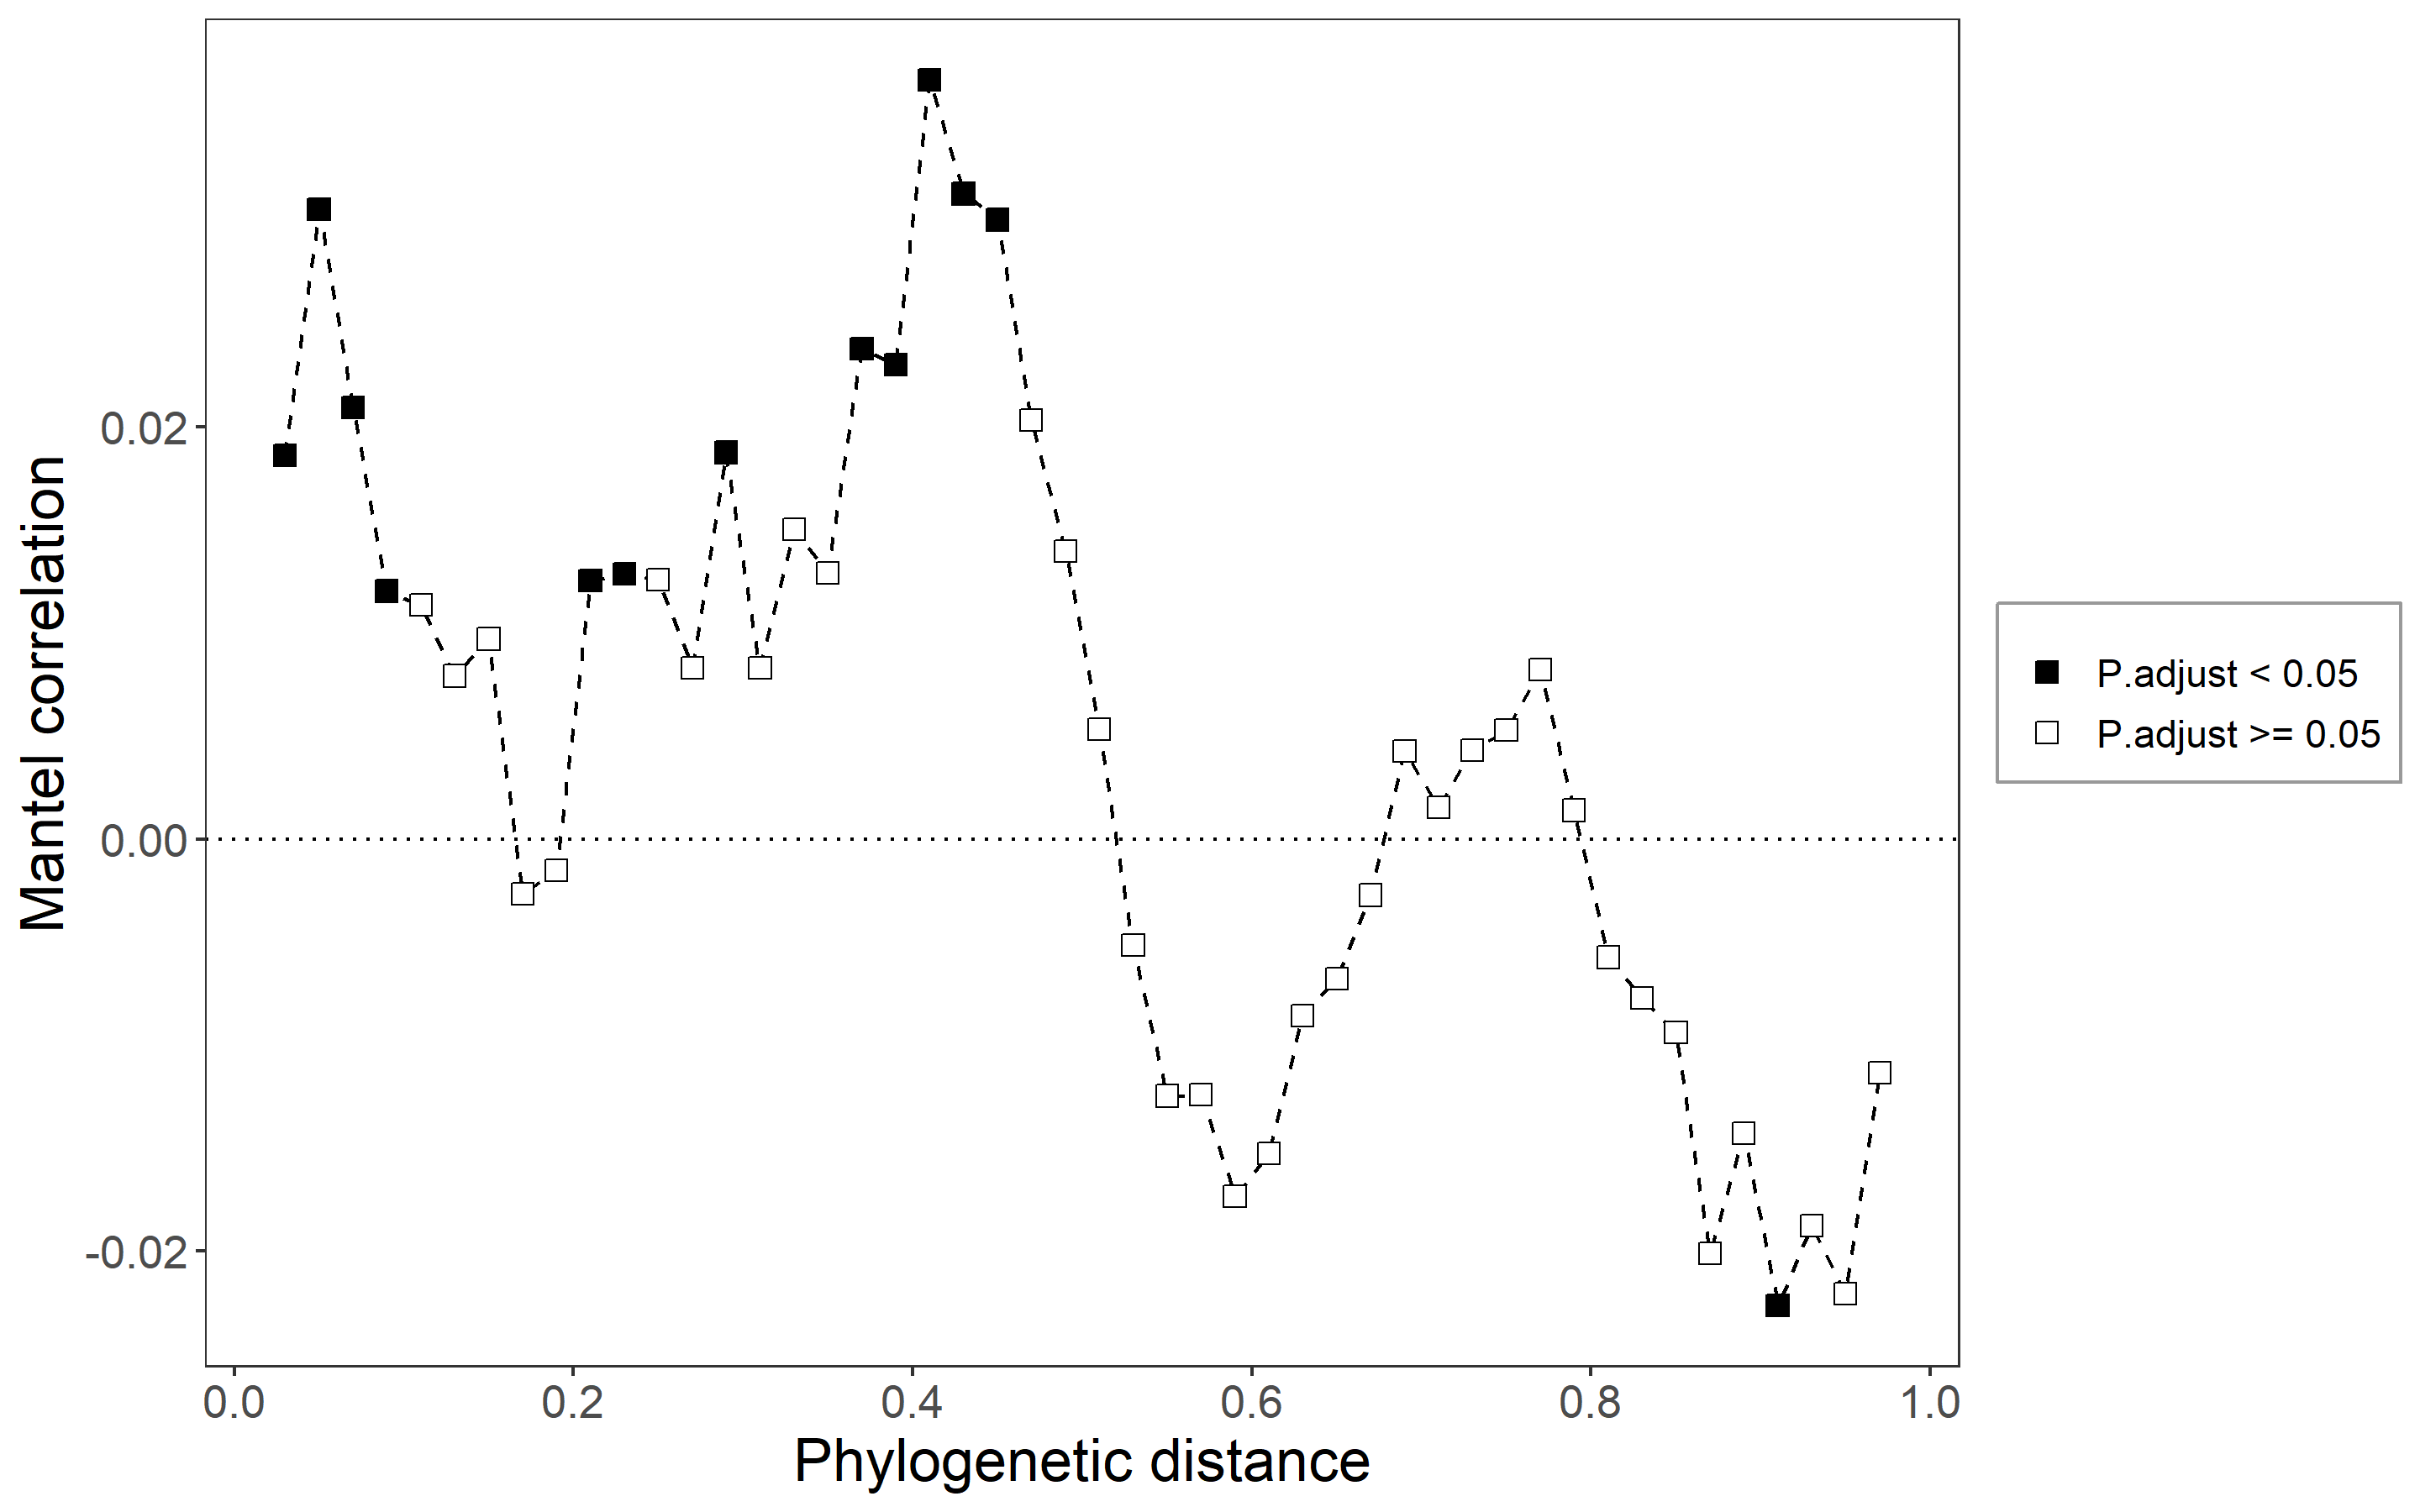
\includegraphics[width=600px]{Images/trans_nullmodel_mantel_corr} \end{center}

betaNRI(ses.betampd) is used to show the `basal' phylogenetic turnover.
Compared to betaNTI, it can capture more turnover information associated with the deep phylogeny.
It is noted that there are many null models with the development in the several decades of community ecology.
In the trans\_nullmodel class,
the default null mode of betaNTI and betaNRI is the randomization of the phylogenetic relatedness among species.
This shuffling approach fix the observed levels of species α-diversity and β-diversity to
explore whether the observed phylogenetic turnover significantly differ from null model that phylogenetic relatedness among species are random.

\begin{Shaded}
\begin{Highlighting}[]
\CommentTok{\# see null.model parameter for other null models}
\CommentTok{\# null model run 500 times for the example}
\NormalTok{t1}\SpecialCharTok{$}\FunctionTok{cal\_ses\_betampd}\NormalTok{(}\AttributeTok{runs =} \DecValTok{500}\NormalTok{, }\AttributeTok{abundance.weighted =} \ConstantTok{TRUE}\NormalTok{)}
\CommentTok{\# return t1$res\_ses\_betampd}
\end{Highlighting}
\end{Shaded}

If we want to plot the betaNRI, we can use plot\_group\_distance function in trans\_beta class.
For example, the results showed that the mean betaNRI of TW is extremely and significantly larger that those in CW and IW,
revealing that the basal phylogenetic turnover in TW is high.

\begin{Shaded}
\begin{Highlighting}[]
\CommentTok{\# add betaNRI matrix to beta\_diversity list}
\NormalTok{dataset}\SpecialCharTok{$}\NormalTok{beta\_diversity[[}\StringTok{"betaNRI"}\NormalTok{]] }\OtherTok{\textless{}{-}}\NormalTok{ t1}\SpecialCharTok{$}\NormalTok{res\_ses\_betampd}
\CommentTok{\# create trans\_beta class, use measure "betaNRI"}
\NormalTok{t2 }\OtherTok{\textless{}{-}}\NormalTok{ trans\_beta}\SpecialCharTok{$}\FunctionTok{new}\NormalTok{(}\AttributeTok{dataset =}\NormalTok{ dataset, }\AttributeTok{group =} \StringTok{"Group"}\NormalTok{, }\AttributeTok{measure =} \StringTok{"betaNRI"}\NormalTok{)}
\CommentTok{\# transform the distance for each group}
\NormalTok{t2}\SpecialCharTok{$}\FunctionTok{cal\_group\_distance}\NormalTok{()}
\CommentTok{\# see the help document for more methods, e.g. "anova" and "KW\_dunn"}
\NormalTok{t2}\SpecialCharTok{$}\FunctionTok{cal\_group\_distance\_diff}\NormalTok{(}\AttributeTok{method =} \StringTok{"wilcox"}\NormalTok{)}
\CommentTok{\# plot the results}
\NormalTok{g1 }\OtherTok{\textless{}{-}}\NormalTok{ t2}\SpecialCharTok{$}\FunctionTok{plot\_group\_distance}\NormalTok{(}\AttributeTok{boxplot\_add =} \StringTok{"mean"}\NormalTok{)}
\NormalTok{g1 }\SpecialCharTok{+} \FunctionTok{geom\_hline}\NormalTok{(}\AttributeTok{yintercept =} \SpecialCharTok{{-}}\DecValTok{2}\NormalTok{, }\AttributeTok{linetype =} \DecValTok{2}\NormalTok{) }\SpecialCharTok{+} \FunctionTok{geom\_hline}\NormalTok{(}\AttributeTok{yintercept =} \DecValTok{2}\NormalTok{, }\AttributeTok{linetype =} \DecValTok{2}\NormalTok{)}
\end{Highlighting}
\end{Shaded}

\begin{center}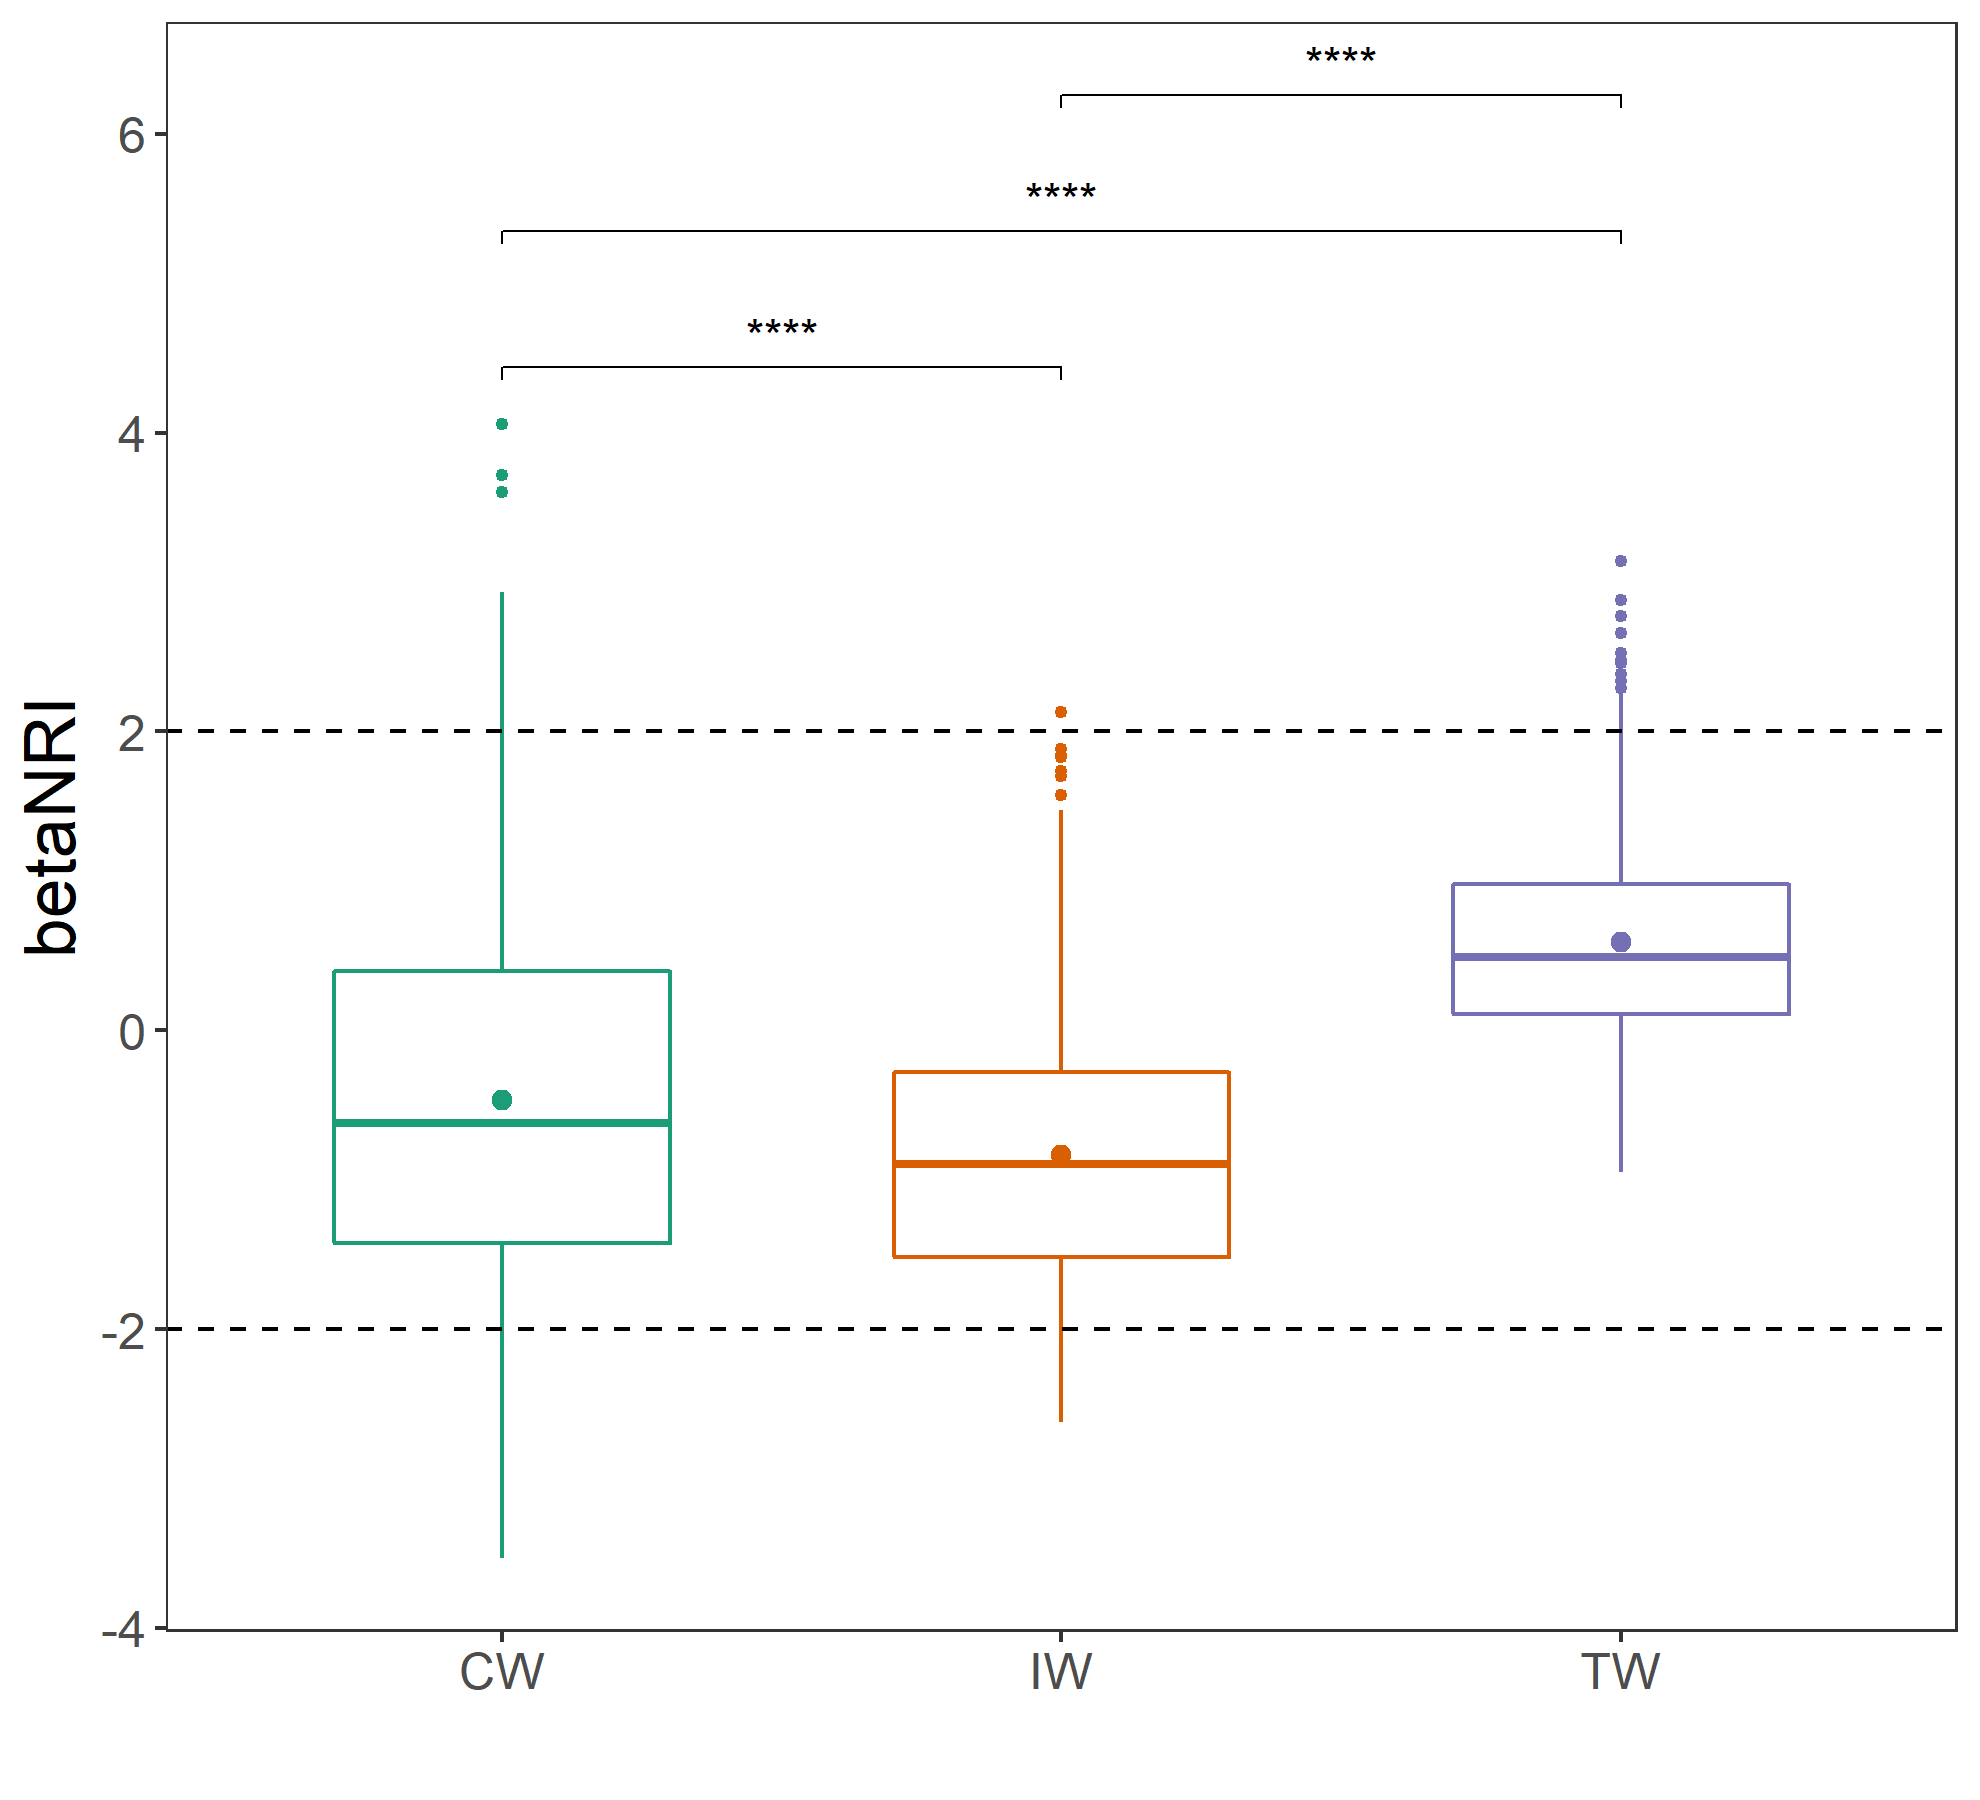
\includegraphics[width=550px]{Images/trans_nullmodel_betaNRI_one_dataset} \end{center}

Sometimes, if you want to perform null model analysis for each group individually, such as one group as one species pool,
you should calculate the results for each group, respectively.
The results show that, when we perform betaNRI for each group respectively,
mean betaNRI between CW and TW are not significantly different, and they are both significantly higher than that in IW,
revealing that the strength of variable selection in CW and TW may be similar under the condition that each area is considered as a specific species pool.

\begin{Shaded}
\begin{Highlighting}[]
\CommentTok{\# we create a list to store the trans\_nullmodel results.}
\NormalTok{sesbeta\_each }\OtherTok{\textless{}{-}} \FunctionTok{list}\NormalTok{()}
\NormalTok{group\_col }\OtherTok{\textless{}{-}} \StringTok{"Group"}
\NormalTok{all\_groups }\OtherTok{\textless{}{-}} \FunctionTok{unique}\NormalTok{(dataset}\SpecialCharTok{$}\NormalTok{sample\_table[, group\_col])}
\CommentTok{\# calculate for each group, respectively}
\ControlFlowTok{for}\NormalTok{(i }\ControlFlowTok{in}\NormalTok{ all\_groups)\{}
    \CommentTok{\# like the above operation, but need provide \textquotesingle{}group\textquotesingle{} and \textquotesingle{}select\_group\textquotesingle{}}
\NormalTok{    test }\OtherTok{\textless{}{-}}\NormalTok{ trans\_nullmodel}\SpecialCharTok{$}\FunctionTok{new}\NormalTok{(dataset, }\AttributeTok{group =}\NormalTok{ group\_col, }\AttributeTok{select\_group =}\NormalTok{ i, }\AttributeTok{filter\_thres =} \FloatTok{0.0005}\NormalTok{)}
\NormalTok{    test}\SpecialCharTok{$}\FunctionTok{cal\_ses\_betampd}\NormalTok{(}\AttributeTok{runs =} \DecValTok{500}\NormalTok{, }\AttributeTok{abundance.weighted =} \ConstantTok{TRUE}\NormalTok{)}
\NormalTok{    sesbeta\_each[[i]] }\OtherTok{\textless{}{-}}\NormalTok{ test}\SpecialCharTok{$}\NormalTok{res\_ses\_betampd}
\NormalTok{\}}
\CommentTok{\# merge and reshape to generate one symmetrical matrix}
\NormalTok{test }\OtherTok{\textless{}{-}} \FunctionTok{lapply}\NormalTok{(sesbeta\_each, reshape2}\SpecialCharTok{::}\NormalTok{melt) }\SpecialCharTok{\%\textgreater{}\%} 
    \FunctionTok{do.call}\NormalTok{(rbind, .) }\SpecialCharTok{\%\textgreater{}\%}
\NormalTok{    reshape2}\SpecialCharTok{::}\FunctionTok{dcast}\NormalTok{(., Var1}\SpecialCharTok{\textasciitilde{}}\NormalTok{Var2, }\AttributeTok{value.var =} \StringTok{"value"}\NormalTok{)}
\FunctionTok{rownames}\NormalTok{(test) }\OtherTok{\textless{}{-}}\NormalTok{ test[, }\DecValTok{1}\NormalTok{]}
\NormalTok{test }\OtherTok{\textless{}{-}}\NormalTok{ test[, }\SpecialCharTok{{-}}\DecValTok{1}\NormalTok{, drop }\OtherTok{=} \ConstantTok{FALSE}\NormalTok{]}
\CommentTok{\# like the above operation}
\NormalTok{dataset}\SpecialCharTok{$}\NormalTok{beta\_diversity[[}\StringTok{"betaNRI"}\NormalTok{]] }\OtherTok{\textless{}{-}}\NormalTok{ test}
\NormalTok{t2 }\OtherTok{\textless{}{-}}\NormalTok{ trans\_beta}\SpecialCharTok{$}\FunctionTok{new}\NormalTok{(}\AttributeTok{dataset =}\NormalTok{ dataset, }\AttributeTok{group =} \StringTok{"Group"}\NormalTok{, }\AttributeTok{measure =} \StringTok{"betaNRI"}\NormalTok{)}
\NormalTok{t2}\SpecialCharTok{$}\FunctionTok{cal\_group\_distance}\NormalTok{()}
\CommentTok{\# statistical analysis}
\NormalTok{t2}\SpecialCharTok{$}\FunctionTok{cal\_group\_distance\_diff}\NormalTok{(}\AttributeTok{method =} \StringTok{"wilcox"}\NormalTok{)}
\NormalTok{g1 }\OtherTok{\textless{}{-}}\NormalTok{ t2}\SpecialCharTok{$}\FunctionTok{plot\_group\_distance}\NormalTok{(}\AttributeTok{boxplot\_add =} \StringTok{"mean"}\NormalTok{)}
\NormalTok{g1 }\SpecialCharTok{+} \FunctionTok{geom\_hline}\NormalTok{(}\AttributeTok{yintercept =} \SpecialCharTok{{-}}\DecValTok{2}\NormalTok{, }\AttributeTok{linetype =} \DecValTok{2}\NormalTok{) }\SpecialCharTok{+} \FunctionTok{geom\_hline}\NormalTok{(}\AttributeTok{yintercept =} \DecValTok{2}\NormalTok{, }\AttributeTok{linetype =} \DecValTok{2}\NormalTok{)}
\end{Highlighting}
\end{Shaded}

\begin{center}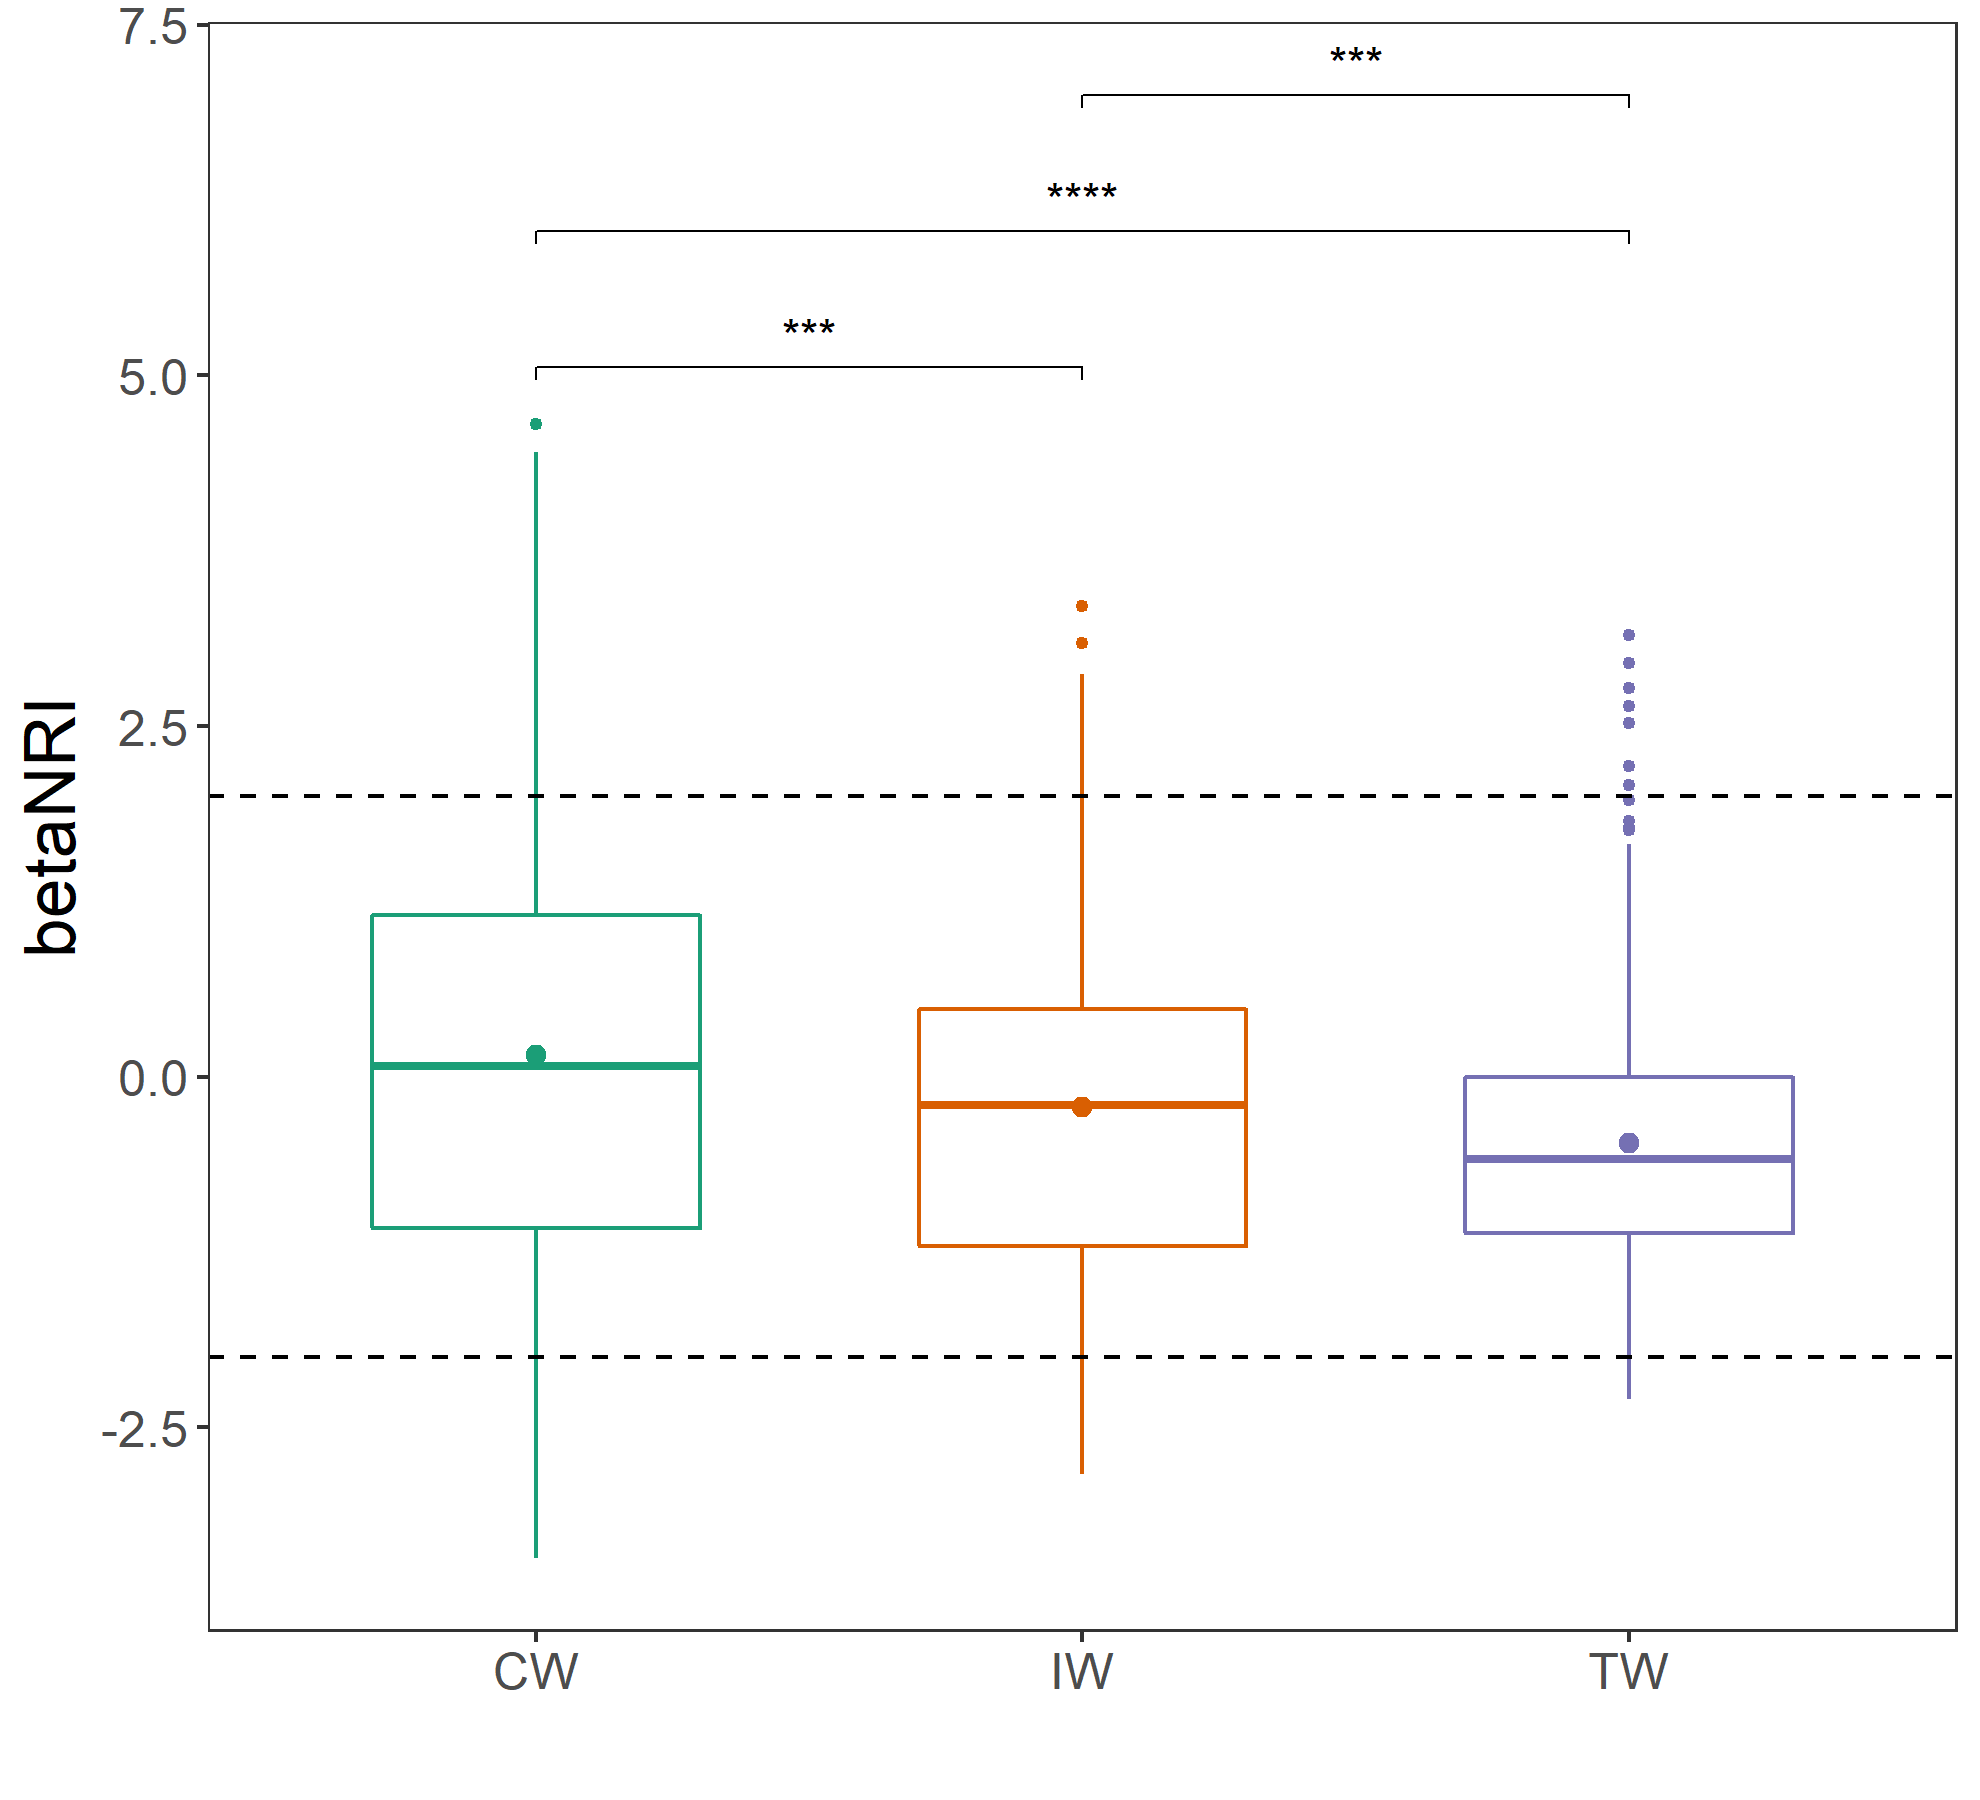
\includegraphics[width=550px]{Images/trans_nullmodel_betaNRI_each_dataset} \end{center}

BetaNTI(ses.betamntd) can be used to indicate the phylogenetic terminal turnover \citep{Stegen_Quantifying_2013}.

\begin{Shaded}
\begin{Highlighting}[]
\CommentTok{\# null model run 500 times}
\NormalTok{t1}\SpecialCharTok{$}\FunctionTok{cal\_ses\_betamntd}\NormalTok{(}\AttributeTok{runs =} \DecValTok{500}\NormalTok{, }\AttributeTok{abundance.weighted =} \ConstantTok{TRUE}\NormalTok{, }\AttributeTok{null.model =} \StringTok{"taxa.labels"}\NormalTok{)}
\CommentTok{\# return t1$res\_ses\_betamntd}
\end{Highlighting}
\end{Shaded}

\begin{longtable}[]{@{}
  >{\centering\arraybackslash}p{(\columnwidth - 10\tabcolsep) * \real{0.1250}}
  >{\centering\arraybackslash}p{(\columnwidth - 10\tabcolsep) * \real{0.1389}}
  >{\centering\arraybackslash}p{(\columnwidth - 10\tabcolsep) * \real{0.1389}}
  >{\centering\arraybackslash}p{(\columnwidth - 10\tabcolsep) * \real{0.1389}}
  >{\centering\arraybackslash}p{(\columnwidth - 10\tabcolsep) * \real{0.1250}}
  >{\centering\arraybackslash}p{(\columnwidth - 10\tabcolsep) * \real{0.1389}}@{}}
\toprule()
\begin{minipage}[b]{\linewidth}\centering
~
\end{minipage} & \begin{minipage}[b]{\linewidth}\centering
S1
\end{minipage} & \begin{minipage}[b]{\linewidth}\centering
S2
\end{minipage} & \begin{minipage}[b]{\linewidth}\centering
S3
\end{minipage} & \begin{minipage}[b]{\linewidth}\centering
S4
\end{minipage} & \begin{minipage}[b]{\linewidth}\centering
S5
\end{minipage} \\
\midrule()
\endhead
\textbf{S1} & 0 & -0.432 & -0.7318 & 0.6482 & 1.236 \\
\textbf{S2} & -0.432 & 0 & -0.9817 & 0.1372 & 0.8991 \\
\textbf{S3} & -0.7318 & -0.9817 & 0 & 1.098 & 0.02069 \\
\textbf{S4} & 0.6482 & 0.1372 & 1.098 & 0 & -1.085 \\
\textbf{S5} & 1.236 & 0.8991 & 0.02069 & -1.085 & 0 \\
\bottomrule()
\end{longtable}

If the dataset is large, it is faster with use\_iCAMP = TRUE for betaNTI.

\begin{Shaded}
\begin{Highlighting}[]
\NormalTok{tmp }\OtherTok{\textless{}{-}} \StringTok{"./test1"}\NormalTok{; }\FunctionTok{dir.create}\NormalTok{(tmp)}
\NormalTok{t1}\SpecialCharTok{$}\FunctionTok{cal\_ses\_betamntd}\NormalTok{(}\AttributeTok{runs =} \DecValTok{1000}\NormalTok{, }\AttributeTok{abundance.weighted =} \ConstantTok{TRUE}\NormalTok{, }\AttributeTok{use\_iCAMP =} \ConstantTok{TRUE}\NormalTok{, }\AttributeTok{iCAMP\_tempdir =}\NormalTok{ tmp)}
\end{Highlighting}
\end{Shaded}

RCbray (Bray-Curtis-based Raup-Crick) can be calculated using function cal\_rcbray()
to assess whether the compositional turnover was governed primarily by drift \citep{Chase_null_2011}.
We applied null model to simulate species distribution by randomly sampling individuals from each
species pool with preserving species occurrence frequency and sample species richness \citep{Liu_Long_term_2017}.

\begin{Shaded}
\begin{Highlighting}[]
\CommentTok{\# result stored in t1$res\_rcbray}
\NormalTok{t1}\SpecialCharTok{$}\FunctionTok{cal\_rcbray}\NormalTok{(}\AttributeTok{runs =} \DecValTok{1000}\NormalTok{)}
\CommentTok{\# return t1$res\_rcbray}
\end{Highlighting}
\end{Shaded}

As an example, we also calculate the proportion of the inferred processes on the community assembly as shown in the references \citep{Stegen_Quantifying_2013, Liu_Long_term_2017}.
In the example, the fraction of pairwise comparisons with significant betaNTI values (\textbar βNTI\textbar{} \textgreater{} 2) is the estimated influence of Selection;
βNTI \textgreater{} 2 represents the heterogeneous selection; βNTI \textless{} -2 represents the homogeneous selection.
The value of RCbray characterizes the magnitude of deviation between observed Bray--Curtis and Bray--Curtis expected under the randomization;
a value of \textbar RCbray\textbar{} \textgreater{} 0.95 was considered significant.
The fraction of all pairwise comparisons with \textbar βNTI\textbar{} \textless{} 2 and RCbray \textgreater{} +0.95 was taken as the influence of Dispersal Limitation combined with Drift.
The fraction of all pairwise comparisons with \textbar βNTI\textbar{} \textless{} 2 and RCbray \textless{} -0.95 was taken as an estimate for the influence of Homogenizing Dispersal.
The fraction of all pairwise comparisons with \textbar βNTI\textbar{} \textless{} 2 and \textbar RCbray\textbar{} \textless{} 0.95 estimates the influence of Drift acting alone.

\begin{Shaded}
\begin{Highlighting}[]
\CommentTok{\# use betaNTI and rcbray to evaluate processes}
\NormalTok{t1}\SpecialCharTok{$}\FunctionTok{cal\_process}\NormalTok{(}\AttributeTok{use\_betamntd =} \ConstantTok{TRUE}\NormalTok{)}
\end{Highlighting}
\end{Shaded}

\begin{verbatim}
## The result is stored in object$res_process ...
\end{verbatim}

\begin{Shaded}
\begin{Highlighting}[]
\CommentTok{\# return t1$res\_process}
\end{Highlighting}
\end{Shaded}

\begin{Shaded}
\begin{Highlighting}[]
\NormalTok{t1}\SpecialCharTok{$}\NormalTok{res\_process}
\end{Highlighting}
\end{Shaded}

\begin{longtable}[]{@{}
  >{\centering\arraybackslash}p{(\columnwidth - 2\tabcolsep) * \real{0.3333}}
  >{\centering\arraybackslash}p{(\columnwidth - 2\tabcolsep) * \real{0.1806}}@{}}
\toprule()
\begin{minipage}[b]{\linewidth}\centering
process
\end{minipage} & \begin{minipage}[b]{\linewidth}\centering
percentage
\end{minipage} \\
\midrule()
\endhead
variable selection & 9.238 \\
homogeneous selection & 0 \\
dispersal limitation & 8.964 \\
homogeneous dispersal & 11.54 \\
drift & 70.26 \\
\bottomrule()
\end{longtable}

The \texttt{cal\_NST} function can be used to calculate normalized stochasticity ratio based on the NST package \citep{Ning_general_2019},
including `tNST' and `pNST' methods.

\begin{Shaded}
\begin{Highlighting}[]
\CommentTok{\# require NST package to be installed}
\NormalTok{t1}\SpecialCharTok{$}\FunctionTok{cal\_NST}\NormalTok{(}\AttributeTok{method =} \StringTok{"tNST"}\NormalTok{, }\AttributeTok{group =} \StringTok{"Group"}\NormalTok{, }\AttributeTok{dist.method =} \StringTok{"bray"}\NormalTok{, }\AttributeTok{abundance.weighted =} \ConstantTok{TRUE}\NormalTok{, }\AttributeTok{output.rand =} \ConstantTok{TRUE}\NormalTok{, }\AttributeTok{SES =} \ConstantTok{TRUE}\NormalTok{)}
\NormalTok{t1}\SpecialCharTok{$}\NormalTok{res\_NST}\SpecialCharTok{$}\NormalTok{index.grp}
\end{Highlighting}
\end{Shaded}

\begin{verbatim}
## Perform tNST analysis ...
\end{verbatim}

\begin{verbatim}
## All match very well.
\end{verbatim}

\begin{verbatim}
## Now randomizing by parallel computing. Begin at Fri Dec 22 15:22:59 2023. Please wait...
\end{verbatim}

\begin{verbatim}
## The result is stored in object$res_NST ...
\end{verbatim}

\begin{longtable}[]{@{}
  >{\centering\arraybackslash}p{(\columnwidth - 10\tabcolsep) * \real{0.1111}}
  >{\centering\arraybackslash}p{(\columnwidth - 10\tabcolsep) * \real{0.0972}}
  >{\centering\arraybackslash}p{(\columnwidth - 10\tabcolsep) * \real{0.1667}}
  >{\centering\arraybackslash}p{(\columnwidth - 10\tabcolsep) * \real{0.1806}}
  >{\centering\arraybackslash}p{(\columnwidth - 10\tabcolsep) * \real{0.1806}}
  >{\centering\arraybackslash}p{(\columnwidth - 10\tabcolsep) * \real{0.1806}}@{}}
\toprule()
\begin{minipage}[b]{\linewidth}\centering
group
\end{minipage} & \begin{minipage}[b]{\linewidth}\centering
size
\end{minipage} & \begin{minipage}[b]{\linewidth}\centering
ST.i.bray
\end{minipage} & \begin{minipage}[b]{\linewidth}\centering
NST.i.bray
\end{minipage} & \begin{minipage}[b]{\linewidth}\centering
MST.i.bray
\end{minipage} & \begin{minipage}[b]{\linewidth}\centering
SES.i.bray
\end{minipage} \\
\midrule()
\endhead
IW & 435 & 0.6537 & 0.3869 & 0.3638 & 9.105 \\
CW & 435 & 0.5633 & 0.297 & 0.2867 & 14.24 \\
TW & 435 & 0.6247 & 0.4163 & 0.4001 & 9.836 \\
\bottomrule()
\end{longtable}

\begin{Shaded}
\begin{Highlighting}[]
\CommentTok{\# test the NST difference between each pair of groups}
\NormalTok{t1}\SpecialCharTok{$}\FunctionTok{cal\_NST\_test}\NormalTok{(}\AttributeTok{method =} \StringTok{"nst.boot"}\NormalTok{)}
\end{Highlighting}
\end{Shaded}

\begin{Shaded}
\begin{Highlighting}[]
\CommentTok{\# convert long format table to square matrix}
\CommentTok{\# the 10th column: MST.ij.bray in t1$res\_NST$index.pair}
\NormalTok{test }\OtherTok{\textless{}{-}}\NormalTok{ t1}\SpecialCharTok{$}\FunctionTok{cal\_NST\_convert}\NormalTok{(}\DecValTok{10}\NormalTok{)}
\end{Highlighting}
\end{Shaded}

\begin{Shaded}
\begin{Highlighting}[]
\CommentTok{\# for pNST method, phylogenetic tree is needed}
\NormalTok{t1}\SpecialCharTok{$}\FunctionTok{cal\_NST}\NormalTok{(}\AttributeTok{method =} \StringTok{"pNST"}\NormalTok{, }\AttributeTok{group =} \StringTok{"Group"}\NormalTok{, }\AttributeTok{output.rand =} \ConstantTok{TRUE}\NormalTok{, }\AttributeTok{SES =} \ConstantTok{TRUE}\NormalTok{)}
\NormalTok{t1}\SpecialCharTok{$}\FunctionTok{cal\_NST\_test}\NormalTok{(}\AttributeTok{method =} \StringTok{"nst.boot"}\NormalTok{)}
\end{Highlighting}
\end{Shaded}

For nearest Taxon Index (NTI) and nearest Relative Index (NRI), please use cal\_NTI and cal\_NRI, respectively.

\begin{Shaded}
\begin{Highlighting}[]
\NormalTok{t1}\SpecialCharTok{$}\FunctionTok{cal\_NRI}\NormalTok{(}\AttributeTok{null.model =} \StringTok{"taxa.labels"}\NormalTok{, }\AttributeTok{abundance.weighted =} \ConstantTok{FALSE}\NormalTok{, }\AttributeTok{runs =} \DecValTok{999}\NormalTok{)}
\NormalTok{t1}\SpecialCharTok{$}\FunctionTok{cal\_NTI}\NormalTok{(}\AttributeTok{null.model =} \StringTok{"taxa.labels"}\NormalTok{, }\AttributeTok{abundance.weighted =} \ConstantTok{TRUE}\NormalTok{, }\AttributeTok{runs =} \DecValTok{999}\NormalTok{)}
\end{Highlighting}
\end{Shaded}

\hypertarget{key-points-7}{%
\subsection{Key points}\label{key-points-7}}

\begin{itemize}
\tightlist
\item
  trans\_nullmodel\$new: filter\_thres parameter for the filtering of taxa with relative low abundance
\item
  cal\_rcbray(): if only need rcbray, ignore other phylogenetic operations
\end{itemize}

\hypertarget{other-function}{%
\subsection{Other function}\label{other-function}}

\begin{itemize}
\tightlist
\item
  cal\_Cscore(): calculates the (normalised) mean number of checkerboard combinations (C-score) using C.score
\end{itemize}

\hypertarget{trans_classifier-class}{%
\section{trans\_classifier class}\label{trans_classifier-class}}

The trans\_classifier class is a wrapper for methods of machine-learning-based classification models.
Microbiome-based supervised machine-learning has been successful in predicting human health status \citep{Poore_Microbiome_2020}
and soil categories \citep{Wilhelm_Predicting_2021}.

\hypertarget{dependencies}{%
\subsection{Dependencies}\label{dependencies}}

Before starting the examples, make sure those packages have been installed.

\begin{Shaded}
\begin{Highlighting}[]
\NormalTok{packages }\OtherTok{\textless{}{-}} \FunctionTok{c}\NormalTok{(}\StringTok{"Boruta"}\NormalTok{, }\StringTok{"parallel"}\NormalTok{, }\StringTok{"rsample"}\NormalTok{, }\StringTok{"randomForest"}\NormalTok{, }\StringTok{"caret"}\NormalTok{, }\StringTok{"gridExtra"}\NormalTok{, }\StringTok{"multiROC"}\NormalTok{)}
\CommentTok{\# Now check or install}
\ControlFlowTok{for}\NormalTok{(x }\ControlFlowTok{in}\NormalTok{ packages)\{}
    \ControlFlowTok{if}\NormalTok{(}\SpecialCharTok{!}\FunctionTok{require}\NormalTok{(x, }\AttributeTok{character.only =} \ConstantTok{TRUE}\NormalTok{)) \{}
        \FunctionTok{install.packages}\NormalTok{(x, }\AttributeTok{dependencies =} \ConstantTok{TRUE}\NormalTok{)}
\NormalTok{    \}}
\NormalTok{\}}
\end{Highlighting}
\end{Shaded}

\hypertarget{examples}{%
\subsection{Examples}\label{examples}}

In this section, we use the example data in file2meco package (\url{https://chiliubio.github.io/microeco_tutorial/file2meco-package.html}) to demonstrate the feature selection,
data training and prediction with random forest algorithm.

\begin{Shaded}
\begin{Highlighting}[]
\FunctionTok{library}\NormalTok{(file2meco)}
\NormalTok{abund\_file\_path }\OtherTok{\textless{}{-}} \FunctionTok{system.file}\NormalTok{(}\StringTok{"extdata"}\NormalTok{, }\StringTok{"dada2\_table.qza"}\NormalTok{, }\AttributeTok{package=}\StringTok{"file2meco"}\NormalTok{)}
\NormalTok{sample\_file\_path }\OtherTok{\textless{}{-}} \FunctionTok{system.file}\NormalTok{(}\StringTok{"extdata"}\NormalTok{, }\StringTok{"sample{-}metadata.tsv"}\NormalTok{, }\AttributeTok{package=}\StringTok{"file2meco"}\NormalTok{)}
\NormalTok{taxonomy\_file\_path }\OtherTok{\textless{}{-}} \FunctionTok{system.file}\NormalTok{(}\StringTok{"extdata"}\NormalTok{, }\StringTok{"taxonomy.qza"}\NormalTok{, }\AttributeTok{package=}\StringTok{"file2meco"}\NormalTok{)}
\CommentTok{\# construct microtable object}
\NormalTok{d1 }\OtherTok{\textless{}{-}} \FunctionTok{qiime2meco}\NormalTok{(}\AttributeTok{feature\_table =}\NormalTok{ abund\_file\_path, }\AttributeTok{sample\_table =}\NormalTok{ sample\_file\_path, }\AttributeTok{taxonomy\_table =}\NormalTok{ taxonomy\_file\_path)}
\NormalTok{d1}\SpecialCharTok{$}\FunctionTok{cal\_abund}\NormalTok{()}

\CommentTok{\# initialize: use "genotype" as response variable}
\CommentTok{\# x.predictors parameter is used to select the taxa; here we use all the taxa data in d1$taxa\_abund}
\NormalTok{t1 }\OtherTok{\textless{}{-}}\NormalTok{ trans\_classifier}\SpecialCharTok{$}\FunctionTok{new}\NormalTok{(}\AttributeTok{dataset =}\NormalTok{ d1, }\AttributeTok{y.response =} \StringTok{"genotype"}\NormalTok{, }\AttributeTok{x.predictors =} \StringTok{"All"}\NormalTok{)}
\end{Highlighting}
\end{Shaded}

We silit the data into training and testing set.

\begin{Shaded}
\begin{Highlighting}[]
\CommentTok{\# generate train and test set}
\NormalTok{t1}\SpecialCharTok{$}\FunctionTok{cal\_split}\NormalTok{(}\AttributeTok{prop.train =} \DecValTok{3}\SpecialCharTok{/}\DecValTok{4}\NormalTok{)}
\end{Highlighting}
\end{Shaded}

Before training the model, we run the set\_trainControl to invoke the trainControl function of caret package to generate the parameters used for training.
Here we use the default parameters in trainControl function.

\begin{Shaded}
\begin{Highlighting}[]
\CommentTok{\# require caret package}
\NormalTok{t1}\SpecialCharTok{$}\FunctionTok{set\_trainControl}\NormalTok{()}
\end{Highlighting}
\end{Shaded}

Now let's start model training with rf method.

\begin{Shaded}
\begin{Highlighting}[]
\CommentTok{\# use default parameter method = "rf"}
\NormalTok{t1}\SpecialCharTok{$}\FunctionTok{cal\_train}\NormalTok{(}\AttributeTok{max.ntree =} \DecValTok{500}\NormalTok{)}
\end{Highlighting}
\end{Shaded}

We can use cal\_predict function to predict the testing data set.

\begin{Shaded}
\begin{Highlighting}[]
\NormalTok{t1}\SpecialCharTok{$}\FunctionTok{cal\_predict}\NormalTok{()}
\CommentTok{\# plot the confusionMatrix to check out the performance}
\NormalTok{t1}\SpecialCharTok{$}\FunctionTok{plot\_confusionMatrix}\NormalTok{()}
\end{Highlighting}
\end{Shaded}

\begin{center}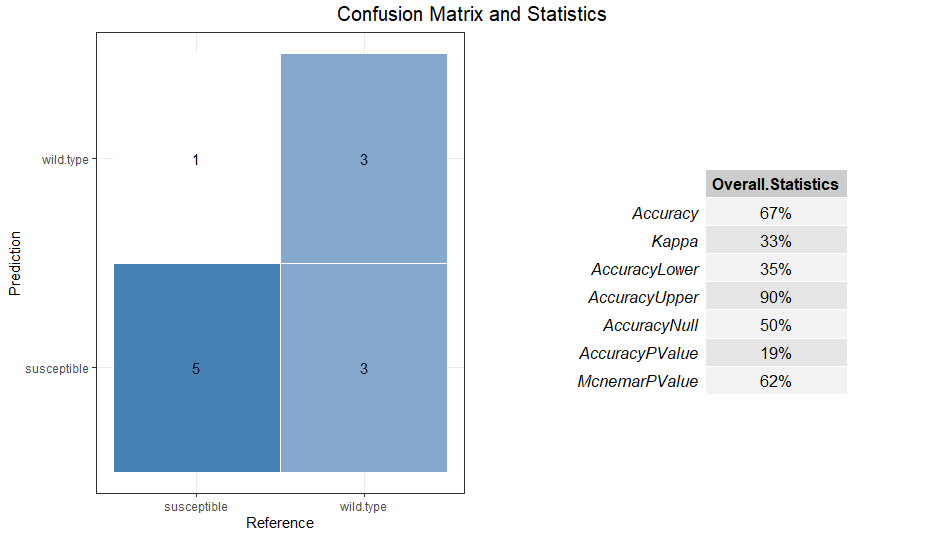
\includegraphics[width=600px]{Images/plot_confusionMatrix_without_selection} \end{center}

Using cal\_ROC and plot\_ROC can get the ROC (Receiver Operator Characteristic) curve.

\begin{Shaded}
\begin{Highlighting}[]
\NormalTok{t1}\SpecialCharTok{$}\FunctionTok{cal\_ROC}\NormalTok{()}
\NormalTok{t1}\SpecialCharTok{$}\FunctionTok{plot\_ROC}\NormalTok{(}\AttributeTok{size =} \FloatTok{0.5}\NormalTok{, }\AttributeTok{alpha =} \FloatTok{0.7}\NormalTok{)}
\end{Highlighting}
\end{Shaded}

\begin{center}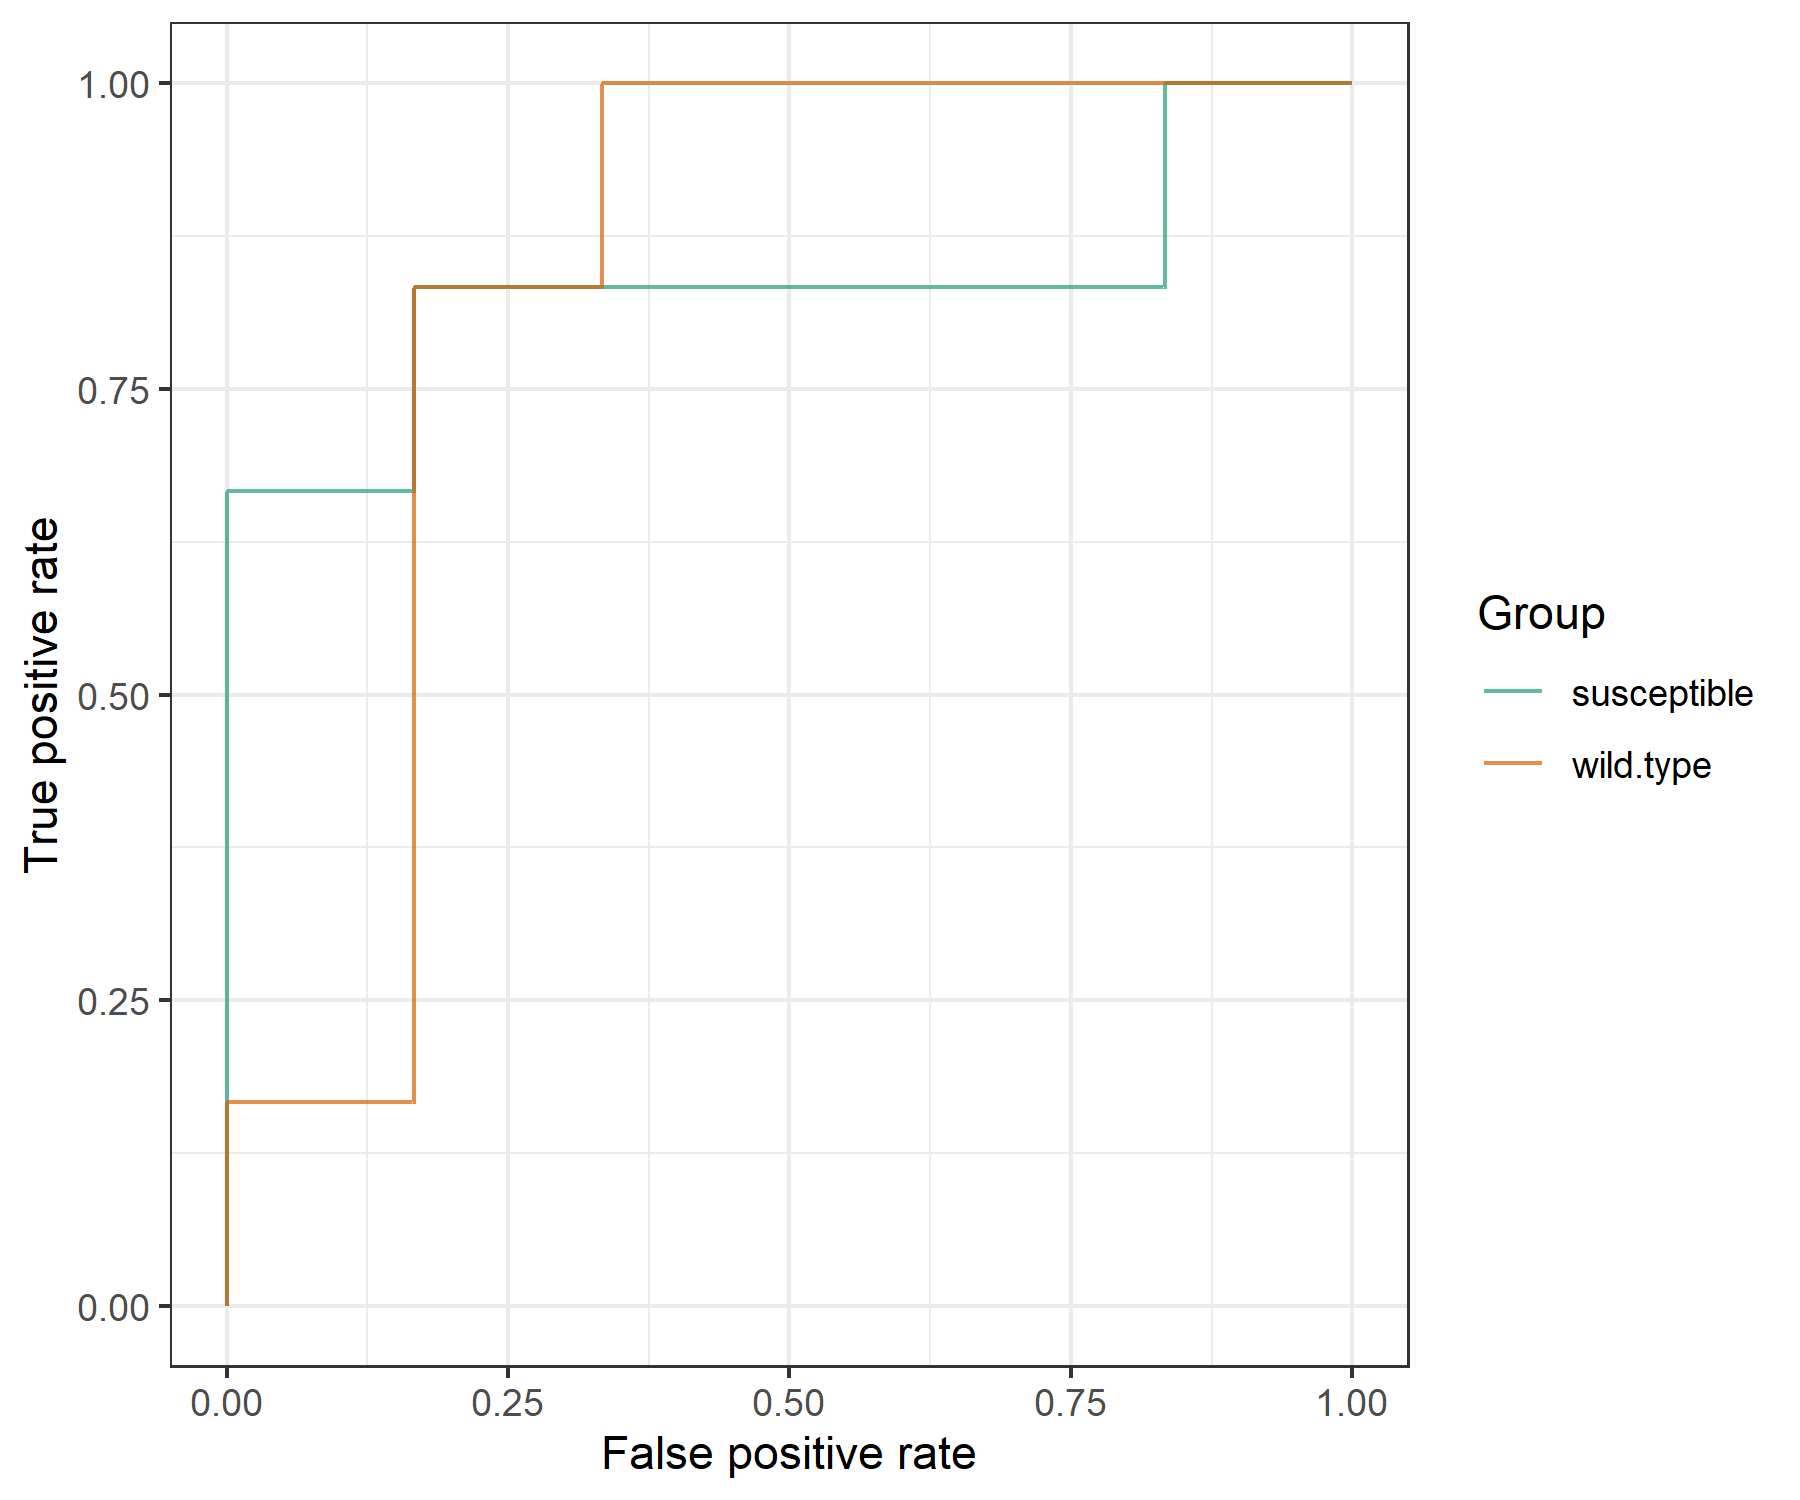
\includegraphics[width=500px]{Images/plot_ROC_without_selection} \end{center}

While building a machine learning model for microbiome data,
the huge diversity of microbial community and/or associated relationships among taxa accross phylogeny can lead to a large number of unnecessary features,
which can reduce the overall accuracy, increase the complexity and overfit of the model and decrease the generalization capability of the model.
So, feature selection is one important step in building machine-learning model.
Then, we attempt to use Boruta package \citep{Kursa_Feature_2010} to do feature selection.

\begin{Shaded}
\begin{Highlighting}[]
\CommentTok{\# require Boruta package}
\NormalTok{t1}\SpecialCharTok{$}\FunctionTok{cal\_feature\_sel}\NormalTok{(}\AttributeTok{boruta.maxRuns =} \DecValTok{300}\NormalTok{, }\AttributeTok{boruta.pValue =} \FloatTok{0.01}\NormalTok{)}
\end{Highlighting}
\end{Shaded}

To compare the results between the procedure with feature selection and that without feature selection,
we also perfom all the analysis with feature selection to show the whole results.

\begin{Shaded}
\begin{Highlighting}[]
\NormalTok{t2 }\OtherTok{\textless{}{-}}\NormalTok{ trans\_classifier}\SpecialCharTok{$}\FunctionTok{new}\NormalTok{(}\AttributeTok{dataset =}\NormalTok{ d1, }\AttributeTok{y.response =} \StringTok{"genotype"}\NormalTok{, }\AttributeTok{x.predictors =} \StringTok{"All"}\NormalTok{)}
\NormalTok{t2}\SpecialCharTok{$}\FunctionTok{cal\_feature\_sel}\NormalTok{(}\AttributeTok{boruta.maxRuns =} \DecValTok{300}\NormalTok{, }\AttributeTok{boruta.pValue =} \FloatTok{0.01}\NormalTok{)}
\NormalTok{t2}\SpecialCharTok{$}\FunctionTok{cal\_split}\NormalTok{(}\AttributeTok{prop.train =} \DecValTok{3}\SpecialCharTok{/}\DecValTok{4}\NormalTok{)}
\NormalTok{t2}\SpecialCharTok{$}\FunctionTok{set\_trainControl}\NormalTok{()}
\NormalTok{t2}\SpecialCharTok{$}\FunctionTok{cal\_train}\NormalTok{(}\AttributeTok{max.ntree =} \DecValTok{500}\NormalTok{)}
\NormalTok{t2}\SpecialCharTok{$}\FunctionTok{cal\_predict}\NormalTok{()}
\NormalTok{t2}\SpecialCharTok{$}\FunctionTok{plot\_confusionMatrix}\NormalTok{()}
\NormalTok{t2}\SpecialCharTok{$}\FunctionTok{cal\_ROC}\NormalTok{()}
\NormalTok{t2}\SpecialCharTok{$}\FunctionTok{plot\_ROC}\NormalTok{(}\AttributeTok{size =} \FloatTok{0.5}\NormalTok{, }\AttributeTok{alpha =} \FloatTok{0.7}\NormalTok{)}
\end{Highlighting}
\end{Shaded}

\begin{center}\includegraphics[width=600px]{Images/plot_confusionMatrix_with_selection} \end{center}

\begin{center}\includegraphics[width=500px]{Images/plot_ROC_with_selection} \end{center}

To plot the Precision-Recall curve (PR curve), please make plot\_type = ``PR'' in plot\_ROC function.

\begin{Shaded}
\begin{Highlighting}[]
\NormalTok{t2}\SpecialCharTok{$}\FunctionTok{plot\_ROC}\NormalTok{(}\AttributeTok{plot\_type =} \StringTok{"PR"}\NormalTok{, }\AttributeTok{size =} \FloatTok{0.5}\NormalTok{, }\AttributeTok{alpha =} \FloatTok{0.7}\NormalTok{)}
\end{Highlighting}
\end{Shaded}

\begin{center}\includegraphics[width=500px]{Images/plot_PR_with_selection} \end{center}

To show the ROC curve or PR curve of the training result, please make input = ``train'' in plot\_ROC function.

\begin{Shaded}
\begin{Highlighting}[]
\NormalTok{t2}\SpecialCharTok{$}\FunctionTok{cal\_ROC}\NormalTok{(}\AttributeTok{input =} \StringTok{"train"}\NormalTok{)}
\NormalTok{t2}\SpecialCharTok{$}\FunctionTok{plot\_ROC}\NormalTok{(}\AttributeTok{plot\_type =} \StringTok{"ROC"}\NormalTok{, }\AttributeTok{size =} \FloatTok{0.5}\NormalTok{, }\AttributeTok{alpha =} \FloatTok{0.7}\NormalTok{)}
\end{Highlighting}
\end{Shaded}

\begin{center}\includegraphics[width=500px]{Images/plot_ROC_with_selection_training} \end{center}

For other machine-learning models, please use method parameter in cal\_train function.

\begin{Shaded}
\begin{Highlighting}[]
\CommentTok{\# use SVM method}
\NormalTok{t2}\SpecialCharTok{$}\FunctionTok{al\_train}\NormalTok{(}\AttributeTok{method =} \StringTok{"svmRadial"}\NormalTok{, }\AttributeTok{tuneLength =} \DecValTok{15}\NormalTok{)}
\end{Highlighting}
\end{Shaded}

The regression is supported from v0.15.0.

\begin{Shaded}
\begin{Highlighting}[]
\CommentTok{\# prepare data}
\FunctionTok{data}\NormalTok{(env\_data\_16S)}
\NormalTok{new\_test }\OtherTok{\textless{}{-}} \FunctionTok{clone}\NormalTok{(dataset)}
\NormalTok{new\_test}\SpecialCharTok{$}\NormalTok{sample\_table }\OtherTok{\textless{}{-}} \FunctionTok{data.frame}\NormalTok{(new\_test}\SpecialCharTok{$}\NormalTok{sample\_table, env\_data\_16S[}\FunctionTok{rownames}\NormalTok{(new\_test}\SpecialCharTok{$}\NormalTok{sample\_table), ])}
\CommentTok{\# pH response variable}
\NormalTok{t1 }\OtherTok{\textless{}{-}}\NormalTok{ trans\_classifier}\SpecialCharTok{$}\FunctionTok{new}\NormalTok{(}\AttributeTok{dataset =}\NormalTok{ new\_test, }\AttributeTok{y.response =} \StringTok{"pH"}\NormalTok{, }\AttributeTok{x.predictors =} \StringTok{"Genus"}\NormalTok{)}
\NormalTok{t1}\SpecialCharTok{$}\FunctionTok{cal\_split}\NormalTok{(}\AttributeTok{prop.train =} \DecValTok{3}\SpecialCharTok{/}\DecValTok{4}\NormalTok{)}
\NormalTok{t1}\SpecialCharTok{$}\FunctionTok{set\_trainControl}\NormalTok{()}
\NormalTok{t1}\SpecialCharTok{$}\FunctionTok{cal\_train}\NormalTok{()}
\NormalTok{t1}\SpecialCharTok{$}\NormalTok{res\_train}
\NormalTok{t1}\SpecialCharTok{$}\FunctionTok{cal\_predict}\NormalTok{()}
\NormalTok{t1}\SpecialCharTok{$}\NormalTok{res\_predict}
\CommentTok{\# feature importance}
\NormalTok{t1}\SpecialCharTok{$}\FunctionTok{cal\_feature\_imp}\NormalTok{()}
\FunctionTok{head}\NormalTok{(t1}\SpecialCharTok{$}\NormalTok{res\_feature\_imp)}
\NormalTok{t1}\SpecialCharTok{$}\FunctionTok{plot\_feature\_imp}\NormalTok{(}\AttributeTok{use\_number =} \DecValTok{1}\SpecialCharTok{:}\DecValTok{20}\NormalTok{) }\SpecialCharTok{+} \FunctionTok{ylab}\NormalTok{(}\StringTok{"IncNodePurity"}\NormalTok{)}
\end{Highlighting}
\end{Shaded}

\hypertarget{key-points-8}{%
\subsection{Key points}\label{key-points-8}}

\begin{itemize}
\tightlist
\item
  cal\_feature\_sel(): perform feature selection
\end{itemize}

\hypertarget{other-function-1}{%
\subsection{Other function}\label{other-function-1}}

\begin{itemize}
\tightlist
\item
  cal\_feature\_imp(): get feature importance from the training model when method is ``rf''
\item
  cal\_preProcess(): Pre-process (centering, scaling etc.) of the feature data based on the caret::preProcess function.
\end{itemize}

\hypertarget{explainable-class}{%
\chapter{Explainable class}\label{explainable-class}}

The trans\_env and trans\_func classes are placed into the section `Explainable class',
as environmental factors and microbial functions can be generally applied to explain microbial community structure and assembly.

\hypertarget{trans_env-class}{%
\section{trans\_env class}\label{trans_env-class}}

There may be some NA (missing value) in the user's env data.
If so, please add \texttt{complete\_na\ =\ TRUE} for the interpolation when creating a trans\_env object.

\hypertarget{example-7}{%
\subsection{Example}\label{example-7}}

Creating trans\_env object has at least two ways.
The following is using additional environmental data which is not in the microtable object.

\begin{Shaded}
\begin{Highlighting}[]
\CommentTok{\# add\_data is used to add the environmental data}
\NormalTok{t1 }\OtherTok{\textless{}{-}}\NormalTok{ trans\_env}\SpecialCharTok{$}\FunctionTok{new}\NormalTok{(}\AttributeTok{dataset =}\NormalTok{ dataset, }\AttributeTok{add\_data =}\NormalTok{ env\_data\_16S[, }\DecValTok{4}\SpecialCharTok{:}\DecValTok{11}\NormalTok{])}
\end{Highlighting}
\end{Shaded}

\begin{verbatim}
## Env data is stored in object$data_env ...
\end{verbatim}

Maybe a more general way is to directly use the data from sample\_table of your microtable object.
To show this operation, we first merge additional table into sample\_table to generate a new microtable object.

\begin{Shaded}
\begin{Highlighting}[]
\NormalTok{new\_test }\OtherTok{\textless{}{-}} \FunctionTok{clone}\NormalTok{(dataset)}
\NormalTok{new\_test}\SpecialCharTok{$}\NormalTok{sample\_table }\OtherTok{\textless{}{-}} \FunctionTok{data.frame}\NormalTok{(new\_test}\SpecialCharTok{$}\NormalTok{sample\_table, env\_data\_16S[}\FunctionTok{rownames}\NormalTok{(new\_test}\SpecialCharTok{$}\NormalTok{sample\_table), ])}
\CommentTok{\# now new\_test$sample\_table has the whole data}
\NormalTok{new\_test}
\end{Highlighting}
\end{Shaded}

\begin{verbatim}
## microtable-class object:
## sample_table have 90 rows and 15 columns
## otu_table have 12766 rows and 90 columns
## tax_table have 12766 rows and 7 columns
## phylo_tree have 12766 tips
## Taxa abundance: calculated for Kingdom,Phylum,Class,Order,Family,Genus,Species 
## Alpha diversity: calculated for Observed,Chao1,se.chao1,ACE,se.ACE,Shannon,Simpson,InvSimpson,Fisher,Coverage 
## Beta diversity: calculated for bray,jaccard
\end{verbatim}

Now let's use env\_cols to select the required columns from sample\_table in the microtable object.
From v1.0.0, the parameter \texttt{standardize\ =\ TRUE} is available to standardize each variable.

\begin{Shaded}
\begin{Highlighting}[]
\NormalTok{t1 }\OtherTok{\textless{}{-}}\NormalTok{ trans\_env}\SpecialCharTok{$}\FunctionTok{new}\NormalTok{(}\AttributeTok{dataset =}\NormalTok{ new\_test, }\AttributeTok{env\_cols =} \DecValTok{8}\SpecialCharTok{:}\DecValTok{15}\NormalTok{)}
\end{Highlighting}
\end{Shaded}

\begin{verbatim}
## Env data is stored in object$data_env ...
\end{verbatim}

Generally, it is beneficial to analyze environmental variables in order to better use more methods.
The \texttt{cal\_diff} function is used to test the significance of variables across groups like we have shown in trans\_alpha and trans\_diff class parts.

\begin{Shaded}
\begin{Highlighting}[]
\CommentTok{\# use Wilcoxon Rank Sum Test as an example}
\NormalTok{t1}\SpecialCharTok{$}\FunctionTok{cal\_diff}\NormalTok{(}\AttributeTok{group =} \StringTok{"Group"}\NormalTok{, }\AttributeTok{method =} \StringTok{"wilcox"}\NormalTok{)}
\FunctionTok{head}\NormalTok{(t1}\SpecialCharTok{$}\NormalTok{res\_diff)}
\end{Highlighting}
\end{Shaded}

\begin{verbatim}
## The result is stored in object$res_diff ...
\end{verbatim}

\begin{longtable}[]{@{}
  >{\centering\arraybackslash}p{(\columnwidth - 8\tabcolsep) * \real{0.1806}}
  >{\centering\arraybackslash}p{(\columnwidth - 8\tabcolsep) * \real{0.2222}}
  >{\centering\arraybackslash}p{(\columnwidth - 8\tabcolsep) * \real{0.1111}}
  >{\centering\arraybackslash}p{(\columnwidth - 8\tabcolsep) * \real{0.1667}}
  >{\centering\arraybackslash}p{(\columnwidth - 8\tabcolsep) * \real{0.2083}}@{}}
\toprule()
\begin{minipage}[b]{\linewidth}\centering
Comparison
\end{minipage} & \begin{minipage}[b]{\linewidth}\centering
Measure
\end{minipage} & \begin{minipage}[b]{\linewidth}\centering
Group
\end{minipage} & \begin{minipage}[b]{\linewidth}\centering
P.adj
\end{minipage} & \begin{minipage}[b]{\linewidth}\centering
Significance
\end{minipage} \\
\midrule()
\endhead
IW - CW & Temperature & CW & 3.283e-10 & *** \\
IW - TW & Temperature & TW & 0.0001958 & *** \\
CW - TW & Temperature & CW & 3.283e-10 & *** \\
IW - CW & Precipitation & CW & 5.239e-09 & *** \\
IW - TW & Precipitation & IW & 0.07758 & ns \\
CW - TW & Precipitation & CW & 4.002e-07 & *** \\
IW - CW & TOC & IW & 0.4687 & ns \\
\bottomrule()
\end{longtable}

Let's perform the ANOVA and show the letters in the box plot. We use list to store all the plots for each factor and plot them together.

\begin{Shaded}
\begin{Highlighting}[]
\NormalTok{t1}\SpecialCharTok{$}\FunctionTok{cal\_diff}\NormalTok{(}\AttributeTok{method =} \StringTok{"anova"}\NormalTok{, }\AttributeTok{group =} \StringTok{"Group"}\NormalTok{)}
\CommentTok{\# place all the plots into a list}
\NormalTok{tmp }\OtherTok{\textless{}{-}} \FunctionTok{list}\NormalTok{()}
\ControlFlowTok{for}\NormalTok{(i }\ControlFlowTok{in} \FunctionTok{colnames}\NormalTok{(t1}\SpecialCharTok{$}\NormalTok{data\_env))\{}
\NormalTok{    tmp[[i]] }\OtherTok{\textless{}{-}}\NormalTok{ t1}\SpecialCharTok{$}\FunctionTok{plot\_diff}\NormalTok{(}\AttributeTok{measure =}\NormalTok{ i, }\AttributeTok{add\_sig\_text\_size =} \DecValTok{5}\NormalTok{, }\AttributeTok{xtext\_size =} \DecValTok{12}\NormalTok{) }\SpecialCharTok{+} \FunctionTok{theme}\NormalTok{(}\AttributeTok{plot.margin =} \FunctionTok{unit}\NormalTok{(}\FunctionTok{c}\NormalTok{(}\FloatTok{0.1}\NormalTok{, }\DecValTok{0}\NormalTok{, }\DecValTok{0}\NormalTok{, }\DecValTok{1}\NormalTok{), }\StringTok{"cm"}\NormalTok{))}
\NormalTok{\}}
\FunctionTok{plot}\NormalTok{(gridExtra}\SpecialCharTok{::}\FunctionTok{arrangeGrob}\NormalTok{(}\AttributeTok{grobs =}\NormalTok{ tmp, }\AttributeTok{ncol =} \DecValTok{3}\NormalTok{))}
\end{Highlighting}
\end{Shaded}

\begin{center}\includegraphics[width=750px]{Images/trans_env_diff_all} \end{center}

From v0.12.0, trans\_env class supports the differential test of groups within each group by using the by\_group parameter in cal\_diff function.

\begin{Shaded}
\begin{Highlighting}[]
\NormalTok{t1}\SpecialCharTok{$}\FunctionTok{cal\_diff}\NormalTok{(}\AttributeTok{group =} \StringTok{"Type"}\NormalTok{, }\AttributeTok{by\_group =} \StringTok{"Group"}\NormalTok{, }\AttributeTok{method =} \StringTok{"anova"}\NormalTok{)}
\NormalTok{t1}\SpecialCharTok{$}\FunctionTok{plot\_diff}\NormalTok{(}\AttributeTok{measure =} \StringTok{"pH"}\NormalTok{, }\AttributeTok{add\_sig\_text\_size =} \DecValTok{5}\NormalTok{)}
\end{Highlighting}
\end{Shaded}

\begin{center}\includegraphics[width=600px]{Images/trans_env_diff_bygroup} \end{center}

Then we show the autocorrelations among variables.

\begin{Shaded}
\begin{Highlighting}[]
\CommentTok{\# require GGally package to be installed}
\NormalTok{t1}\SpecialCharTok{$}\FunctionTok{cal\_autocor}\NormalTok{()}
\end{Highlighting}
\end{Shaded}

\begin{center}\includegraphics[width=800px]{Images/trans_env_autocor1} \end{center}

For different groups, please use group parameter to show the distributions of variables and the autocorrelations across groups.

\begin{Shaded}
\begin{Highlighting}[]
\NormalTok{t1}\SpecialCharTok{$}\FunctionTok{cal\_autocor}\NormalTok{(}\AttributeTok{group =} \StringTok{"Group"}\NormalTok{)}
\end{Highlighting}
\end{Shaded}

\begin{center}\includegraphics[width=800px]{Images/trans_env_autocor_group} \end{center}

Then let's show the RDA analysis (db-RDA and RDA).

\begin{Shaded}
\begin{Highlighting}[]
\CommentTok{\# use bray{-}curtis distance for dbRDA}
\NormalTok{t1}\SpecialCharTok{$}\FunctionTok{cal\_ordination}\NormalTok{(}\AttributeTok{method =} \StringTok{"dbRDA"}\NormalTok{, }\AttributeTok{use\_measure =} \StringTok{"bray"}\NormalTok{)}
\CommentTok{\# show the orginal results}
\NormalTok{t1}\SpecialCharTok{$}\FunctionTok{trans\_ordination}\NormalTok{()}
\NormalTok{t1}\SpecialCharTok{$}\FunctionTok{plot\_ordination}\NormalTok{(}\AttributeTok{plot\_color =} \StringTok{"Group"}\NormalTok{)}
\CommentTok{\# the main results of RDA are related with the projection and angles between arrows}
\CommentTok{\# adjust the length of the arrows to show them better}
\NormalTok{t1}\SpecialCharTok{$}\FunctionTok{trans\_ordination}\NormalTok{(}\AttributeTok{adjust\_arrow\_length =} \ConstantTok{TRUE}\NormalTok{, }\AttributeTok{max\_perc\_env =} \FloatTok{1.5}\NormalTok{)}
\CommentTok{\# t1$res\_rda\_trans is the transformed result for plotting}
\NormalTok{t1}\SpecialCharTok{$}\FunctionTok{plot\_ordination}\NormalTok{(}\AttributeTok{plot\_color =} \StringTok{"Group"}\NormalTok{)}
\end{Highlighting}
\end{Shaded}

\begin{center}\includegraphics[width=650px]{Images/trans_env_rda_dbrda} \end{center}

From v0.14.0, the function \texttt{cal\_ordination\_anova} is implemented to check the significance of the ordination model instead of the encapsulation in \texttt{cal\_ordination}.
Furthermore, the function \texttt{cal\_ordination\_envfit} can be used to get the contribution of each variables to the model.

\begin{Shaded}
\begin{Highlighting}[]
\NormalTok{t1}\SpecialCharTok{$}\FunctionTok{cal\_ordination\_anova}\NormalTok{()}
\NormalTok{t1}\SpecialCharTok{$}\FunctionTok{cal\_ordination\_envfit}\NormalTok{()}
\end{Highlighting}
\end{Shaded}

Then, let's try to do RDA at the Genus level.

\begin{Shaded}
\begin{Highlighting}[]
\CommentTok{\# use Genus}
\NormalTok{t1}\SpecialCharTok{$}\FunctionTok{cal\_ordination}\NormalTok{(}\AttributeTok{method =} \StringTok{"RDA"}\NormalTok{, }\AttributeTok{taxa\_level =} \StringTok{"Genus"}\NormalTok{)}
\CommentTok{\# select 10 features and adjust the arrow length}
\NormalTok{t1}\SpecialCharTok{$}\FunctionTok{trans\_ordination}\NormalTok{(}\AttributeTok{show\_taxa =} \DecValTok{10}\NormalTok{, }\AttributeTok{adjust\_arrow\_length =} \ConstantTok{TRUE}\NormalTok{, }\AttributeTok{max\_perc\_env =} \FloatTok{1.5}\NormalTok{, }\AttributeTok{max\_perc\_tax =} \FloatTok{1.5}\NormalTok{, }\AttributeTok{min\_perc\_env =} \FloatTok{0.2}\NormalTok{, }\AttributeTok{min\_perc\_tax =} \FloatTok{0.2}\NormalTok{)}
\CommentTok{\# t1$res\_rda\_trans is the transformed result for plot}
\NormalTok{t1}\SpecialCharTok{$}\FunctionTok{plot\_ordination}\NormalTok{(}\AttributeTok{plot\_color =} \StringTok{"Group"}\NormalTok{)}
\end{Highlighting}
\end{Shaded}

\begin{center}\includegraphics[width=650px]{Images/trans_env_rda_genus} \end{center}

For more visualization styles, run the following examples.

\begin{Shaded}
\begin{Highlighting}[]
\NormalTok{t1}\SpecialCharTok{$}\FunctionTok{plot\_ordination}\NormalTok{(}\AttributeTok{plot\_color =} \StringTok{"Group"}\NormalTok{, }\AttributeTok{plot\_shape =} \StringTok{"Group"}\NormalTok{)}
\NormalTok{t1}\SpecialCharTok{$}\FunctionTok{plot\_ordination}\NormalTok{(}\AttributeTok{plot\_color =} \StringTok{"Group"}\NormalTok{, }\AttributeTok{plot\_shape =} \StringTok{"Group"}\NormalTok{, }\AttributeTok{plot\_type =} \FunctionTok{c}\NormalTok{(}\StringTok{"point"}\NormalTok{, }\StringTok{"ellipse"}\NormalTok{))}
\NormalTok{t1}\SpecialCharTok{$}\FunctionTok{plot\_ordination}\NormalTok{(}\AttributeTok{plot\_color =} \StringTok{"Group"}\NormalTok{, }\AttributeTok{plot\_shape =} \StringTok{"Group"}\NormalTok{, }\AttributeTok{plot\_type =} \FunctionTok{c}\NormalTok{(}\StringTok{"point"}\NormalTok{, }\StringTok{"centroid"}\NormalTok{))}
\NormalTok{t1}\SpecialCharTok{$}\FunctionTok{plot\_ordination}\NormalTok{(}\AttributeTok{plot\_color =} \StringTok{"Group"}\NormalTok{, }\AttributeTok{plot\_shape =} \StringTok{"Group"}\NormalTok{, }\AttributeTok{plot\_type =} \FunctionTok{c}\NormalTok{(}\StringTok{"point"}\NormalTok{, }\StringTok{"chull"}\NormalTok{))}
\NormalTok{t1}\SpecialCharTok{$}\FunctionTok{plot\_ordination}\NormalTok{(}\AttributeTok{plot\_color =} \StringTok{"Group"}\NormalTok{, }\AttributeTok{plot\_shape =} \StringTok{"Group"}\NormalTok{, }\AttributeTok{plot\_type =} \FunctionTok{c}\NormalTok{(}\StringTok{"point"}\NormalTok{, }\StringTok{"ellipse"}\NormalTok{, }\StringTok{"centroid"}\NormalTok{))}
\NormalTok{t1}\SpecialCharTok{$}\FunctionTok{plot\_ordination}\NormalTok{(}\AttributeTok{plot\_color =} \StringTok{"Group"}\NormalTok{, }\AttributeTok{plot\_shape =} \StringTok{"Group"}\NormalTok{, }\AttributeTok{plot\_type =} \FunctionTok{c}\NormalTok{(}\StringTok{"point"}\NormalTok{, }\StringTok{"chull"}\NormalTok{, }\StringTok{"centroid"}\NormalTok{), }\AttributeTok{add\_sample\_label =} \StringTok{"SampleID"}\NormalTok{)}
\NormalTok{t1}\SpecialCharTok{$}\FunctionTok{plot\_ordination}\NormalTok{(}\AttributeTok{plot\_color =} \StringTok{"Group"}\NormalTok{, }\AttributeTok{plot\_shape =} \StringTok{"Group"}\NormalTok{, }\AttributeTok{plot\_type =} \StringTok{"centroid"}\NormalTok{, }\AttributeTok{centroid\_segment\_alpha =} \FloatTok{0.9}\NormalTok{, }\AttributeTok{centroid\_segment\_size =} \DecValTok{1}\NormalTok{, }\AttributeTok{centroid\_segment\_linetype =} \DecValTok{1}\NormalTok{)}
\NormalTok{t1}\SpecialCharTok{$}\FunctionTok{plot\_ordination}\NormalTok{(}\AttributeTok{plot\_color =} \StringTok{"Type"}\NormalTok{, }\AttributeTok{plot\_type =} \FunctionTok{c}\NormalTok{(}\StringTok{"point"}\NormalTok{, }\StringTok{"centroid"}\NormalTok{), }\AttributeTok{centroid\_segment\_linetype =} \DecValTok{1}\NormalTok{)}
\end{Highlighting}
\end{Shaded}

Mantel test can be used to check whether there is significant correlations between environmental variables and distance matrix.

\begin{Shaded}
\begin{Highlighting}[]
\NormalTok{t1}\SpecialCharTok{$}\FunctionTok{cal\_mantel}\NormalTok{(}\AttributeTok{use\_measure =} \StringTok{"bray"}\NormalTok{)}
\CommentTok{\# return t1$res\_mantel}
\FunctionTok{head}\NormalTok{(t1}\SpecialCharTok{$}\NormalTok{res\_mantel)}
\end{Highlighting}
\end{Shaded}

\begin{verbatim}
## The result is stored in object$res_mantel ...
\end{verbatim}

\begin{longtable}[]{@{}
  >{\centering\arraybackslash}p{(\columnwidth - 8\tabcolsep) * \real{0.2000}}
  >{\centering\arraybackslash}p{(\columnwidth - 8\tabcolsep) * \real{0.3250}}
  >{\centering\arraybackslash}p{(\columnwidth - 8\tabcolsep) * \real{0.1250}}
  >{\centering\arraybackslash}p{(\columnwidth - 8\tabcolsep) * \real{0.1625}}
  >{\centering\arraybackslash}p{(\columnwidth - 8\tabcolsep) * \real{0.1875}}@{}}
\toprule()
\begin{minipage}[b]{\linewidth}\centering
Variables
\end{minipage} & \begin{minipage}[b]{\linewidth}\centering
Correlation coefficient
\end{minipage} & \begin{minipage}[b]{\linewidth}\centering
p.value
\end{minipage} & \begin{minipage}[b]{\linewidth}\centering
p.adjusted
\end{minipage} & \begin{minipage}[b]{\linewidth}\centering
Significance
\end{minipage} \\
\midrule()
\endhead
Temperature & 0.452 & 0.001 & 0.002 & ** \\
Precipitation & 0.2791 & 0.001 & 0.002 & ** \\
TOC & 0.13 & 0.003 & 0.004 & ** \\
NH4 & -0.05539 & 0.926 & 0.926 & \\
NO3 & 0.06758 & 0.05 & 0.05714 & \\
pH & 0.4085 & 0.001 & 0.002 & ** \\
Conductivity & 0.2643 & 0.001 & 0.002 & ** \\
TN & 0.1321 & 0.002 & 0.0032 & ** \\
\bottomrule()
\end{longtable}

\begin{Shaded}
\begin{Highlighting}[]
\CommentTok{\# mantel test for different groups}
\NormalTok{t1}\SpecialCharTok{$}\FunctionTok{cal\_mantel}\NormalTok{(}\AttributeTok{by\_group =} \StringTok{"Group"}\NormalTok{, }\AttributeTok{use\_measure =} \StringTok{"bray"}\NormalTok{)}
\CommentTok{\# partial mantel test}
\NormalTok{t1}\SpecialCharTok{$}\FunctionTok{cal\_mantel}\NormalTok{(}\AttributeTok{partial\_mantel =} \ConstantTok{TRUE}\NormalTok{)}
\end{Highlighting}
\end{Shaded}

For the combination of mantel test and correlation heatmap,
please see another example (\url{https://chiliubio.github.io/microeco_tutorial/other-examples-1.html\#mantel-test-correlation-heatmap}).

The correlations between environmental variables and taxa are important in analyzing and inferring the factors affecting community structure.
Let's first perform a correlation heatmap using relative abundance data at Genus level with the \texttt{cal\_cor} function.
The parameter \texttt{p\_adjust\_type} can control the p value adjustment type.

\begin{Shaded}
\begin{Highlighting}[]
\NormalTok{t1 }\OtherTok{\textless{}{-}}\NormalTok{ trans\_env}\SpecialCharTok{$}\FunctionTok{new}\NormalTok{(}\AttributeTok{dataset =}\NormalTok{ dataset, }\AttributeTok{add\_data =}\NormalTok{ env\_data\_16S[, }\DecValTok{4}\SpecialCharTok{:}\DecValTok{11}\NormalTok{])}
\end{Highlighting}
\end{Shaded}

\begin{verbatim}
## Env data is stored in object$data_env ...
\end{verbatim}

\begin{Shaded}
\begin{Highlighting}[]
\CommentTok{\# \textquotesingle{}p\_adjust\_type = "Env"\textquotesingle{} means p adjustment is performed for each environmental variable separately.}
\NormalTok{t1}\SpecialCharTok{$}\FunctionTok{cal\_cor}\NormalTok{(}\AttributeTok{use\_data =} \StringTok{"Genus"}\NormalTok{, }\AttributeTok{p\_adjust\_method =} \StringTok{"fdr"}\NormalTok{, }\AttributeTok{p\_adjust\_type =} \StringTok{"Env"}\NormalTok{)}
\end{Highlighting}
\end{Shaded}

\begin{verbatim}
## The correlation result is stored in object$res_cor ...
\end{verbatim}

\begin{Shaded}
\begin{Highlighting}[]
\CommentTok{\# return t1$res\_cor}
\end{Highlighting}
\end{Shaded}

Then, we can plot the correlation results using plot\_cor function.

\begin{Shaded}
\begin{Highlighting}[]
\CommentTok{\# default ggplot2 method with clustering}
\NormalTok{t1}\SpecialCharTok{$}\FunctionTok{plot\_cor}\NormalTok{()}
\end{Highlighting}
\end{Shaded}

There are too many genera.
We can use the filter\_feature parameter in plot\_cor to filter some taxa that do not have any significance \textless{} 0.001.

\begin{Shaded}
\begin{Highlighting}[]
\CommentTok{\# filter genera that donot have at least one ***}
\NormalTok{t1}\SpecialCharTok{$}\FunctionTok{plot\_cor}\NormalTok{(}\AttributeTok{filter\_feature =} \FunctionTok{c}\NormalTok{(}\StringTok{""}\NormalTok{, }\StringTok{"*"}\NormalTok{, }\StringTok{"**"}\NormalTok{))}
\end{Highlighting}
\end{Shaded}

Sometimes, if the user wants to do the correlation analysis between the environmental factors and some important taxa detected in the biomarker analysis,
please use \textbf{other\_taxa} parameter in cal\_cor function.

\begin{Shaded}
\begin{Highlighting}[]
\CommentTok{\# first create trans\_diff object as a demonstration}
\NormalTok{t2 }\OtherTok{\textless{}{-}}\NormalTok{ trans\_diff}\SpecialCharTok{$}\FunctionTok{new}\NormalTok{(}\AttributeTok{dataset =}\NormalTok{ dataset, }\AttributeTok{method =} \StringTok{"rf"}\NormalTok{, }\AttributeTok{group =} \StringTok{"Group"}\NormalTok{, }\AttributeTok{taxa\_level =} \StringTok{"Genus"}\NormalTok{)}
\CommentTok{\# then create trans\_env object}
\NormalTok{t1 }\OtherTok{\textless{}{-}}\NormalTok{ trans\_env}\SpecialCharTok{$}\FunctionTok{new}\NormalTok{(}\AttributeTok{dataset =}\NormalTok{ dataset, }\AttributeTok{add\_data =}\NormalTok{ env\_data\_16S[, }\DecValTok{4}\SpecialCharTok{:}\DecValTok{11}\NormalTok{])}
\CommentTok{\# use other\_taxa to select taxa you need}
\NormalTok{t1}\SpecialCharTok{$}\FunctionTok{cal\_cor}\NormalTok{(}\AttributeTok{use\_data =} \StringTok{"other"}\NormalTok{, }\AttributeTok{p\_adjust\_method =} \StringTok{"fdr"}\NormalTok{, }\AttributeTok{other\_taxa =}\NormalTok{ t2}\SpecialCharTok{$}\NormalTok{res\_diff}\SpecialCharTok{$}\NormalTok{Taxa[}\DecValTok{1}\SpecialCharTok{:}\DecValTok{40}\NormalTok{])}
\NormalTok{t1}\SpecialCharTok{$}\FunctionTok{plot\_cor}\NormalTok{()}
\end{Highlighting}
\end{Shaded}

\begin{center}\includegraphics[width=700px]{Images/trans_env_corr_ggplot} \end{center}

The pheatmap method is also available.
Note that, besides the \textbf{color\_vector} parameter,
\textbf{color\_palette} can also be used to control color palette with customized colors.

\begin{Shaded}
\begin{Highlighting}[]
\CommentTok{\# clustering heatmap; require pheatmap package}
\CommentTok{\# Let\textquotesingle{}s take another color pallete}
\NormalTok{t1}\SpecialCharTok{$}\FunctionTok{plot\_cor}\NormalTok{(}\AttributeTok{pheatmap =} \ConstantTok{TRUE}\NormalTok{, }\AttributeTok{color\_palette =} \FunctionTok{rev}\NormalTok{(RColorBrewer}\SpecialCharTok{::}\FunctionTok{brewer.pal}\NormalTok{(}\AttributeTok{n =} \DecValTok{9}\NormalTok{, }\AttributeTok{name =} \StringTok{"RdYlBu"}\NormalTok{)))}
\end{Highlighting}
\end{Shaded}

\begin{center}\includegraphics[width=700px]{Images/trans_env_corr_pheatmap} \end{center}

Sometimes, if it is needed to study the correlations between environmental variables and taxa for different groups,
\textbf{by\_group parameter} can be used for this goal.

\begin{Shaded}
\begin{Highlighting}[]
\CommentTok{\# calculate correlations for different groups using parameter by\_group}
\NormalTok{t1}\SpecialCharTok{$}\FunctionTok{cal\_cor}\NormalTok{(}\AttributeTok{by\_group =} \StringTok{"Group"}\NormalTok{, }\AttributeTok{use\_data =} \StringTok{"other"}\NormalTok{, }\AttributeTok{p\_adjust\_method =} \StringTok{"fdr"}\NormalTok{, }\AttributeTok{other\_taxa =}\NormalTok{ t2}\SpecialCharTok{$}\NormalTok{res\_diff}\SpecialCharTok{$}\NormalTok{Taxa[}\DecValTok{1}\SpecialCharTok{:}\DecValTok{40}\NormalTok{])}
\CommentTok{\# return t1$res\_cor}
\NormalTok{t1}\SpecialCharTok{$}\FunctionTok{plot\_cor}\NormalTok{()}
\end{Highlighting}
\end{Shaded}

\begin{center}\includegraphics[width=700px]{Images/trans_env_corr_ggplot_groups} \end{center}

If the user is concerned with the relationship between environmental factors and alpha diversity,
please use \textbf{add\_abund\_table} parameter in the cal\_cor function.

\begin{Shaded}
\begin{Highlighting}[]
\NormalTok{t1 }\OtherTok{\textless{}{-}}\NormalTok{ trans\_env}\SpecialCharTok{$}\FunctionTok{new}\NormalTok{(}\AttributeTok{dataset =}\NormalTok{ dataset, }\AttributeTok{add\_data =}\NormalTok{ env\_data\_16S[, }\DecValTok{4}\SpecialCharTok{:}\DecValTok{11}\NormalTok{])}
\CommentTok{\# use add\_abund\_table parameter to add the extra data table}
\NormalTok{t1}\SpecialCharTok{$}\FunctionTok{cal\_cor}\NormalTok{(}\AttributeTok{add\_abund\_table =}\NormalTok{ dataset}\SpecialCharTok{$}\NormalTok{alpha\_diversity)}
\CommentTok{\# try to use ggplot2 with clustering plot}
\CommentTok{\# require ggtree and aplot packages to be installed (https://chiliubio.github.io/microeco\_tutorial/intro.html\#dependence)}
\NormalTok{t1}\SpecialCharTok{$}\FunctionTok{plot\_cor}\NormalTok{(}\AttributeTok{cluster\_ggplot =} \StringTok{"both"}\NormalTok{)}
\end{Highlighting}
\end{Shaded}

\begin{center}\includegraphics[width=600px]{Images/trans_env_corr_alpha_diversity} \end{center}

The function \texttt{plot\_scatterfit} in trans\_env class is designed for the scatter plot, adding the fitted line and statistics of correlation or regression.

\begin{Shaded}
\begin{Highlighting}[]
\CommentTok{\# use pH and bray{-}curtis distance}
\CommentTok{\# add correlation statistics}
\NormalTok{t1}\SpecialCharTok{$}\FunctionTok{plot\_scatterfit}\NormalTok{(}
    \AttributeTok{x =} \StringTok{"pH"}\NormalTok{, }
    \AttributeTok{y =}\NormalTok{ dataset}\SpecialCharTok{$}\NormalTok{beta\_diversity}\SpecialCharTok{$}\NormalTok{bray[}\FunctionTok{rownames}\NormalTok{(t1}\SpecialCharTok{$}\NormalTok{data\_env), }\FunctionTok{rownames}\NormalTok{(t1}\SpecialCharTok{$}\NormalTok{data\_env)], }
    \AttributeTok{type =} \StringTok{"cor"}\NormalTok{,}
    \AttributeTok{point\_size =} \DecValTok{3}\NormalTok{, }\AttributeTok{point\_alpha =} \FloatTok{0.1}\NormalTok{, }
    \AttributeTok{label.x.npc =} \StringTok{"center"}\NormalTok{, }\AttributeTok{label.y.npc =} \StringTok{"bottom"}\NormalTok{, }
    \AttributeTok{x\_axis\_title =} \StringTok{"Euclidean distance of pH"}\NormalTok{, }
    \AttributeTok{y\_axis\_title =} \StringTok{"Bray{-}Curtis distance"}
\NormalTok{    )}
\end{Highlighting}
\end{Shaded}

\begin{center}\includegraphics[width=550px]{Images/trans_env_scatterfit_cor} \end{center}

\begin{Shaded}
\begin{Highlighting}[]
\CommentTok{\# regression with type = "lm", use group parameter for different groups}
\NormalTok{t1}\SpecialCharTok{$}\FunctionTok{plot\_scatterfit}\NormalTok{(}
    \AttributeTok{x =}\NormalTok{ dataset}\SpecialCharTok{$}\NormalTok{beta\_diversity}\SpecialCharTok{$}\NormalTok{bray[}\FunctionTok{rownames}\NormalTok{(t1}\SpecialCharTok{$}\NormalTok{data\_env), }\FunctionTok{rownames}\NormalTok{(t1}\SpecialCharTok{$}\NormalTok{data\_env)],}
    \AttributeTok{y =} \StringTok{"pH"}\NormalTok{,}
    \AttributeTok{type =} \StringTok{"lm"}\NormalTok{, }
    \AttributeTok{group =} \StringTok{"Group"}\NormalTok{, }
    \AttributeTok{group\_order =} \FunctionTok{c}\NormalTok{(}\StringTok{"CW"}\NormalTok{, }\StringTok{"TW"}\NormalTok{, }\StringTok{"IW"}\NormalTok{),}
    \AttributeTok{point\_size =} \DecValTok{3}\NormalTok{, }\AttributeTok{point\_alpha =} \FloatTok{0.3}\NormalTok{, }\AttributeTok{line\_se =} \ConstantTok{FALSE}\NormalTok{, }\AttributeTok{line\_size =} \FloatTok{1.5}\NormalTok{, }\AttributeTok{shape\_values =} \FunctionTok{c}\NormalTok{(}\DecValTok{16}\NormalTok{, }\DecValTok{17}\NormalTok{, }\DecValTok{7}\NormalTok{),}
    \AttributeTok{y\_axis\_title =} \StringTok{"Euclidean distance of pH"}\NormalTok{, }\AttributeTok{x\_axis\_title =} \StringTok{"Bray{-}Curtis distance"}
\NormalTok{    ) }\SpecialCharTok{+} \FunctionTok{theme}\NormalTok{(}\AttributeTok{axis.title =} \FunctionTok{element\_text}\NormalTok{(}\AttributeTok{size =} \DecValTok{17}\NormalTok{))}
\end{Highlighting}
\end{Shaded}

\begin{center}\includegraphics[width=550px]{Images/trans_env_scatterfit_lmgroup} \end{center}

Other examples.

\begin{Shaded}
\begin{Highlighting}[]
\NormalTok{t1 }\OtherTok{\textless{}{-}}\NormalTok{ trans\_env}\SpecialCharTok{$}\FunctionTok{new}\NormalTok{(}\AttributeTok{dataset =}\NormalTok{ new\_test, }\AttributeTok{env\_cols =} \DecValTok{8}\SpecialCharTok{:}\DecValTok{15}\NormalTok{)}
\CommentTok{\# with forward selection in RDA}
\NormalTok{t1}\SpecialCharTok{$}\FunctionTok{cal\_ordination}\NormalTok{(}\AttributeTok{method =} \StringTok{"dbRDA"}\NormalTok{, }\AttributeTok{feature\_sel =} \ConstantTok{TRUE}\NormalTok{)}
\CommentTok{\# CCA, canonical correspondence analysis}
\NormalTok{t1}\SpecialCharTok{$}\FunctionTok{cal\_ordination}\NormalTok{(}\AttributeTok{method =} \StringTok{"CCA"}\NormalTok{, }\AttributeTok{taxa\_level =} \StringTok{"Genus"}\NormalTok{)}
\NormalTok{t1}\SpecialCharTok{$}\FunctionTok{trans\_ordination}\NormalTok{(}\AttributeTok{adjust\_arrow\_length =} \ConstantTok{TRUE}\NormalTok{)}
\NormalTok{t1}\SpecialCharTok{$}\FunctionTok{plot\_ordination}\NormalTok{(}\AttributeTok{plot\_color =} \StringTok{"Group"}\NormalTok{, }\AttributeTok{plot\_shape =} \StringTok{"Group"}\NormalTok{, }\AttributeTok{plot\_type =} \FunctionTok{c}\NormalTok{(}\StringTok{"point"}\NormalTok{, }\StringTok{"ellipse"}\NormalTok{))}
\CommentTok{\# correlation analysis without p adjustment}
\NormalTok{t1}\SpecialCharTok{$}\FunctionTok{cal\_cor}\NormalTok{(}\AttributeTok{use\_data =} \StringTok{"Genus"}\NormalTok{, }\AttributeTok{p\_adjust\_method =} \StringTok{"none"}\NormalTok{, }\AttributeTok{use\_taxa\_num =} \DecValTok{30}\NormalTok{)}
\CommentTok{\# correlation heatmap with clustering based on the ggplot2 and aplot packages}
\NormalTok{g1 }\OtherTok{\textless{}{-}}\NormalTok{ t1}\SpecialCharTok{$}\FunctionTok{plot\_cor}\NormalTok{(}\AttributeTok{cluster\_ggplot =} \StringTok{"both"}\NormalTok{)}
\NormalTok{g1}
\CommentTok{\# clustering heatmap with ggplot2 depends on aplot package}
\CommentTok{\# to change the detail in the plot, please manipulate each element of g1}
\NormalTok{g1[[}\DecValTok{1}\NormalTok{]]}
\CommentTok{\# standardize x axis text format}
\NormalTok{g1[[}\DecValTok{1}\NormalTok{]] }\OtherTok{\textless{}{-}}\NormalTok{ g1[[}\DecValTok{1}\NormalTok{]] }\SpecialCharTok{+} \FunctionTok{scale\_x\_discrete}\NormalTok{(}\AttributeTok{labels =} \FunctionTok{c}\NormalTok{(}\AttributeTok{NH4 =} \FunctionTok{expression}\NormalTok{(NH[}\DecValTok{4}\NormalTok{]}\SpecialCharTok{\^{}}\StringTok{\textquotesingle{}+\textquotesingle{}}\SpecialCharTok{{-}}\NormalTok{N), }\AttributeTok{NO3 =} \FunctionTok{expression}\NormalTok{(NO[}\DecValTok{3}\NormalTok{]}\SpecialCharTok{\^{}}\StringTok{\textquotesingle{}{-}\textquotesingle{}}\SpecialCharTok{{-}}\NormalTok{N)))}
\NormalTok{g1[[}\DecValTok{1}\NormalTok{]]}
\NormalTok{g1}
\NormalTok{ggplot2}\SpecialCharTok{::}\FunctionTok{ggsave}\NormalTok{(}\StringTok{"test.pdf"}\NormalTok{, g1, }\AttributeTok{width =} \DecValTok{8}\NormalTok{, }\AttributeTok{height =} \DecValTok{6}\NormalTok{)}
\CommentTok{\# For regression, lm\_equation = FALSE can be applied to not display the equation.}
\NormalTok{t1}\SpecialCharTok{$}\FunctionTok{plot\_scatterfit}\NormalTok{(}\AttributeTok{x =} \DecValTok{1}\NormalTok{, }\AttributeTok{y =} \DecValTok{2}\NormalTok{, }\AttributeTok{type =} \StringTok{"lm"}\NormalTok{, }\AttributeTok{lm\_equation =} \ConstantTok{TRUE}\NormalTok{)}
\CommentTok{\# use line\_alpha to adjust the transparency of the confidence interval}
\NormalTok{t1}\SpecialCharTok{$}\FunctionTok{plot\_scatterfit}\NormalTok{(}\AttributeTok{x =} \DecValTok{1}\NormalTok{, }\AttributeTok{y =} \DecValTok{2}\NormalTok{, }\AttributeTok{type =} \StringTok{"lm"}\NormalTok{, }\AttributeTok{lm\_equation =} \ConstantTok{FALSE}\NormalTok{, }\AttributeTok{line\_alpha =} \FloatTok{0.3}\NormalTok{)}
\NormalTok{t1}\SpecialCharTok{$}\FunctionTok{plot\_scatterfit}\NormalTok{(}\AttributeTok{x =} \DecValTok{1}\NormalTok{, }\AttributeTok{y =} \DecValTok{2}\NormalTok{, }\AttributeTok{type =} \StringTok{"lm"}\NormalTok{, }\AttributeTok{point\_alpha =}\NormalTok{ .}\DecValTok{3}\NormalTok{, }\AttributeTok{line\_se =} \ConstantTok{FALSE}\NormalTok{)}
\NormalTok{t1}\SpecialCharTok{$}\FunctionTok{plot\_scatterfit}\NormalTok{(}\AttributeTok{x =} \DecValTok{1}\NormalTok{, }\AttributeTok{y =} \DecValTok{2}\NormalTok{, }\AttributeTok{type =} \StringTok{"lm"}\NormalTok{, }\AttributeTok{line\_se\_color =} \StringTok{"grey90"}\NormalTok{, }\AttributeTok{label\_sep =} \StringTok{","}\NormalTok{, }\AttributeTok{label.x.npc =} \StringTok{"center"}\NormalTok{, }\AttributeTok{label.y.npc =} \StringTok{"bottom"}\NormalTok{)}
\NormalTok{t1}\SpecialCharTok{$}\FunctionTok{plot\_scatterfit}\NormalTok{(}\AttributeTok{x =} \DecValTok{1}\NormalTok{, }\AttributeTok{y =} \DecValTok{2}\NormalTok{, }\AttributeTok{line\_se =} \ConstantTok{FALSE}\NormalTok{, }\AttributeTok{pvalue\_trim =} \DecValTok{3}\NormalTok{, }\AttributeTok{cor\_coef\_trim =} \DecValTok{3}\NormalTok{)}
\NormalTok{t1}\SpecialCharTok{$}\FunctionTok{plot\_scatterfit}\NormalTok{(}\AttributeTok{x =} \StringTok{"pH"}\NormalTok{, }\AttributeTok{y =} \StringTok{"TOC"}\NormalTok{, }\AttributeTok{type =} \StringTok{"lm"}\NormalTok{, }\AttributeTok{group =} \StringTok{"Group"}\NormalTok{, }\AttributeTok{line\_se =} \ConstantTok{FALSE}\NormalTok{, }\AttributeTok{label.x.npc =} \StringTok{"center"}\NormalTok{,}
    \AttributeTok{shape\_values =} \DecValTok{1}\SpecialCharTok{:}\DecValTok{3}\NormalTok{, }\AttributeTok{x\_axis\_title =} \StringTok{"pH"}\NormalTok{, }\AttributeTok{y\_axis\_title =} \StringTok{"TOC"}\NormalTok{)}
\CommentTok{\# correlation between relative abundance of Genus{-}Arthrobacter and pH}
\NormalTok{tmp }\OtherTok{\textless{}{-}} \FunctionTok{unlist}\NormalTok{(dataset}\SpecialCharTok{$}\NormalTok{taxa\_abund}\SpecialCharTok{$}\NormalTok{Genus[}\StringTok{"k\_\_Bacteria|p\_\_Actinobacteria|c\_\_Actinobacteria|o\_\_Micrococcales|f\_\_Micrococcaceae|g\_\_Arthrobacter"}\NormalTok{, ])}
\NormalTok{t1}\SpecialCharTok{$}\FunctionTok{plot\_scatterfit}\NormalTok{(}\AttributeTok{x =} \StringTok{"pH"}\NormalTok{, }\AttributeTok{y =}\NormalTok{ tmp, }\AttributeTok{point\_size =} \DecValTok{3}\NormalTok{, }\AttributeTok{point\_alpha =} \FloatTok{0.3}\NormalTok{, }
    \AttributeTok{y\_axis\_title =} \StringTok{"Arthrobacter"}\NormalTok{, }\AttributeTok{x\_axis\_title =} \StringTok{"pH"}\NormalTok{)}
\end{Highlighting}
\end{Shaded}

\hypertarget{key-points-9}{%
\subsection{Key points}\label{key-points-9}}

\begin{itemize}
\tightlist
\item
  complete\_na parameter in trans\_env\$new: used to fill the NA (missing value) of the environmental data based on the mice package.
\item
  env\_cols parameter in trans\_env\$new: select the variables from sample\_table of your microtable object.
\item
  add\_abund\_table parameter in cal\_cor: other customized data can be also provided for the correlation analysis.
\item
  use\_cor parameter in plot\_scatterfit: both the correlation and regression are available in this function.
\item
  cal\_mantel(): partial\_mantel = TRUE can be used for partial mantel test.
\item
  plot\_ordination(): use plot\_type parameter to select point types and env\_nudge\_x and taxa\_nudge\_x (also \_y) to adjust the text positions.
\end{itemize}

\hypertarget{trans_func-class}{%
\section{trans\_func class}\label{trans_func-class}}

 Ecological researchers are usually interested in the the funtional profiles of microbial communities,
because functional or metabolic data is powerful to explain the structure and dynamics of microbial communities.
As metagenomic sequencing is complicated and expensive, using amplicon sequencing data to predict functional profiles is an alternative choice.
Several software are often used for this goal, such as PICRUSt \citep{Langille_Predictive_2013}, Tax4Fun \citep{Aßhauer_Tax4Fun_2015} and FAPROTAX \citep{Louca_High_2016, Louca_Decoupling_2016}.
These tools are great to be used for the prediction of functional profiles based on the prokaryotic communities from sequencing results.
In addition, it is also important to obtain the traits or functions for each taxa, not just the whole profile of communities.
FAPROTAX database is a collection of the traits and functions of prokaryotes based on the known research results published in books and literatures.
We match the taxonomic information of prokaryotes against this database to predict the traits of prokaryotes on biogeochemical roles.
The NJC19 database \citep{Lim_Large_2020} is also available for animal-associated prokaryotic data, such as human gut microbiota.
We also implement the FUNGuild \citep{Nguyen_FUNGuild_2016} and FungalTraits \citep{Polme_FungalTraits_2020} databases to predict the fungal traits.
The idea identifying prokaryotic traits and functional redundancy was initially inspired by our another study \citep{Liu_Microbial_2022}.

\hypertarget{example-8}{%
\subsection{Example}\label{example-8}}

We first identify/predict traits of taxa with the prokaryotic example data.

\begin{Shaded}
\begin{Highlighting}[]
\CommentTok{\# create object of trans\_func}
\NormalTok{t2 }\OtherTok{\textless{}{-}}\NormalTok{ trans\_func}\SpecialCharTok{$}\FunctionTok{new}\NormalTok{(dataset)}
\CommentTok{\# mapping the taxonomy to the database}
\CommentTok{\# this can recognize prokaryotes or fungi automatically if the names of taxonomic levels are standard.}
\CommentTok{\# for fungi example, see https://chiliubio.github.io/microeco\_tutorial/other{-}dataset.html\#fungi{-}data}
\CommentTok{\# default database for prokaryotes is FAPROTAX database}
\NormalTok{t2}\SpecialCharTok{$}\FunctionTok{cal\_spe\_func}\NormalTok{(}\AttributeTok{prok\_database =} \StringTok{"FAPROTAX"}\NormalTok{)}
\end{Highlighting}
\end{Shaded}

\begin{verbatim}
## FAPROTAX v1.2.6. Please also cite the original FAPROTAX paper: Louca et al. (2016).
\end{verbatim}

\begin{verbatim}
## Decoupling function and taxonomy in the global ocean microbiome. Science, 353(6305), 1272.
\end{verbatim}

\begin{verbatim}
## The functional binary table is stored in object$res_spe_func ...
\end{verbatim}

\begin{Shaded}
\begin{Highlighting}[]
\CommentTok{\# return t2$res\_spe\_func, 1 represent trait exists, 0 represent no or cannot confirmed.}
\end{Highlighting}
\end{Shaded}

\begin{Shaded}
\begin{Highlighting}[]
\NormalTok{t2}\SpecialCharTok{$}\NormalTok{res\_spe\_func[}\DecValTok{1}\SpecialCharTok{:}\DecValTok{5}\NormalTok{, }\DecValTok{1}\SpecialCharTok{:}\DecValTok{2}\NormalTok{]}
\end{Highlighting}
\end{Shaded}

\begin{longtable}[]{@{}
  >{\centering\arraybackslash}p{(\columnwidth - 4\tabcolsep) * \real{0.2083}}
  >{\centering\arraybackslash}p{(\columnwidth - 4\tabcolsep) * \real{0.2222}}
  >{\centering\arraybackslash}p{(\columnwidth - 4\tabcolsep) * \real{0.4167}}@{}}
\toprule()
\begin{minipage}[b]{\linewidth}\centering
~
\end{minipage} & \begin{minipage}[b]{\linewidth}\centering
methanotrophy
\end{minipage} & \begin{minipage}[b]{\linewidth}\centering
acetoclastic\_methanogenesis
\end{minipage} \\
\midrule()
\endhead
\textbf{OTU\_4272} & 0 & 0 \\
\textbf{OTU\_236} & 0 & 0 \\
\textbf{OTU\_399} & 0 & 0 \\
\textbf{OTU\_1556} & 0 & 0 \\
\textbf{OTU\_32} & 0 & 0 \\
\bottomrule()
\end{longtable}

The percentages of the OTUs having the same trait can reflect the functional redundancy of this function in the community.

\begin{Shaded}
\begin{Highlighting}[]
\CommentTok{\# calculate the percentages for communities}
\CommentTok{\# here do not consider the abundance}
\NormalTok{t2}\SpecialCharTok{$}\FunctionTok{cal\_spe\_func\_perc}\NormalTok{(}\AttributeTok{abundance\_weighted =} \ConstantTok{FALSE}\NormalTok{)}
\end{Highlighting}
\end{Shaded}

\begin{verbatim}
## The result table is stored in object$res_spe_func_perc ...
\end{verbatim}

\begin{Shaded}
\begin{Highlighting}[]
\CommentTok{\# t2$res\_spe\_func\_perc[1:5, 1:2]}
\end{Highlighting}
\end{Shaded}

\begin{longtable}[]{@{}
  >{\centering\arraybackslash}p{(\columnwidth - 4\tabcolsep) * \real{0.1250}}
  >{\centering\arraybackslash}p{(\columnwidth - 4\tabcolsep) * \real{0.2222}}
  >{\centering\arraybackslash}p{(\columnwidth - 4\tabcolsep) * \real{0.4167}}@{}}
\toprule()
\begin{minipage}[b]{\linewidth}\centering
~
\end{minipage} & \begin{minipage}[b]{\linewidth}\centering
methanotrophy
\end{minipage} & \begin{minipage}[b]{\linewidth}\centering
acetoclastic\_methanogenesis
\end{minipage} \\
\midrule()
\endhead
\textbf{S1} & 0.39 & 0.04 \\
\textbf{S2} & 0.27 & 0 \\
\textbf{S3} & 0.48 & 0 \\
\textbf{S4} & 0.48 & 0 \\
\textbf{S5} & 0.56 & 0 \\
\bottomrule()
\end{longtable}

From v1.3.0, the \texttt{trans\_spe\_func\_perc} function is implemented to get the long-format table for more flexible manipulation, e.g., filtering and grouping.
The return \texttt{res\_spe\_func\_perc\_trans} in the object is the table for the following visualization.
Note that this step is not necessary as \texttt{plot\_spe\_func\_perc} function can automatically invoke this function if \texttt{res\_spe\_func\_perc\_trans} is not found.

\begin{Shaded}
\begin{Highlighting}[]
\NormalTok{t2}\SpecialCharTok{$}\FunctionTok{trans\_spe\_func\_perc}\NormalTok{()}
\NormalTok{t2}\SpecialCharTok{$}\FunctionTok{plot\_spe\_func\_perc}\NormalTok{()}
\end{Highlighting}
\end{Shaded}

For the differential test of the abundance percentages across groups,
please move to another part (\url{https://chiliubio.github.io/microeco_tutorial/other-examples-1.html\#faprotax-differential-test}).
Then we take another example to show the percentages of the OTUs for each trait in network modules.

\begin{Shaded}
\begin{Highlighting}[]
\CommentTok{\# construct a network for the example}
\NormalTok{network }\OtherTok{\textless{}{-}}\NormalTok{ trans\_network}\SpecialCharTok{$}\FunctionTok{new}\NormalTok{(}\AttributeTok{dataset =}\NormalTok{ dataset, }\AttributeTok{cal\_cor =} \StringTok{"base"}\NormalTok{, }\AttributeTok{taxa\_level =} \StringTok{"OTU"}\NormalTok{, }\AttributeTok{filter\_thres =} \FloatTok{0.0001}\NormalTok{, }\AttributeTok{cor\_method =} \StringTok{"spearman"}\NormalTok{)}
\NormalTok{network}\SpecialCharTok{$}\FunctionTok{cal\_network}\NormalTok{(}\AttributeTok{p\_thres =} \FloatTok{0.01}\NormalTok{, }\AttributeTok{COR\_cut =} \FloatTok{0.7}\NormalTok{)}
\NormalTok{network}\SpecialCharTok{$}\FunctionTok{cal\_module}\NormalTok{()}
\CommentTok{\# convert module info to microtable object}
\NormalTok{meco\_module }\OtherTok{\textless{}{-}}\NormalTok{ network}\SpecialCharTok{$}\FunctionTok{trans\_comm}\NormalTok{(}\AttributeTok{use\_col =} \StringTok{"module"}\NormalTok{)}
\NormalTok{meco\_module\_func }\OtherTok{\textless{}{-}}\NormalTok{ trans\_func}\SpecialCharTok{$}\FunctionTok{new}\NormalTok{(meco\_module)}
\NormalTok{meco\_module\_func}\SpecialCharTok{$}\FunctionTok{cal\_spe\_func}\NormalTok{(}\AttributeTok{prok\_database =} \StringTok{"FAPROTAX"}\NormalTok{)}
\NormalTok{meco\_module\_func}\SpecialCharTok{$}\FunctionTok{cal\_spe\_func\_perc}\NormalTok{(}\AttributeTok{abundance\_weighted =} \ConstantTok{FALSE}\NormalTok{)}
\NormalTok{meco\_module\_func}\SpecialCharTok{$}\FunctionTok{plot\_spe\_func\_perc}\NormalTok{(}\AttributeTok{order\_x =} \FunctionTok{paste0}\NormalTok{(}\StringTok{"M"}\NormalTok{, }\DecValTok{1}\SpecialCharTok{:}\DecValTok{10}\NormalTok{))}
\end{Highlighting}
\end{Shaded}

\begin{center}\includegraphics[width=700px]{Images/plot_func_perc_module} \end{center}

\begin{Shaded}
\begin{Highlighting}[]
\CommentTok{\# If you want to change the group list, reset the list t2$func\_group\_list}
\NormalTok{t2}\SpecialCharTok{$}\NormalTok{func\_group\_list}
\CommentTok{\# use show\_prok\_func to see the detailed information of prokaryotic traits}
\NormalTok{t2}\SpecialCharTok{$}\FunctionTok{show\_prok\_func}\NormalTok{(}\StringTok{"methanotrophy"}\NormalTok{)}
\end{Highlighting}
\end{Shaded}

Then we try to correlate the percentage data in \texttt{res\_spe\_func\_perc} to environmental variables.

\begin{Shaded}
\begin{Highlighting}[]
\NormalTok{t3 }\OtherTok{\textless{}{-}}\NormalTok{ trans\_env}\SpecialCharTok{$}\FunctionTok{new}\NormalTok{(}\AttributeTok{dataset =}\NormalTok{ dataset, }\AttributeTok{add\_data =}\NormalTok{ env\_data\_16S[, }\DecValTok{4}\SpecialCharTok{:}\DecValTok{11}\NormalTok{])}
\NormalTok{t3}\SpecialCharTok{$}\FunctionTok{cal\_cor}\NormalTok{(}\AttributeTok{add\_abund\_table =}\NormalTok{ t2}\SpecialCharTok{$}\NormalTok{res\_spe\_func\_perc, }\AttributeTok{cor\_method =} \StringTok{"spearman"}\NormalTok{)}
\NormalTok{t3}\SpecialCharTok{$}\FunctionTok{plot\_cor}\NormalTok{(}\AttributeTok{pheatmap =} \ConstantTok{TRUE}\NormalTok{)}
\end{Highlighting}
\end{Shaded}

\begin{center}\includegraphics[width=800px]{Images/plot_func_perc_corr} \end{center}

Tax4Fun \citep{Aßhauer_Tax4Fun_2015} requires a strict input file format associated with the taxonomic information.
To analyze the trimmed or changed OTU data in R with Tax4Fun, we provide a link to the Tax4Fun functional prediction.
Please check out the dependence part \url{https://chiliubio.github.io/microeco_tutorial/intro.html\#tax4fun} for installing Tax4Fun package and download SILVA123 ref data.

\begin{Shaded}
\begin{Highlighting}[]
\NormalTok{t1 }\OtherTok{\textless{}{-}}\NormalTok{ trans\_func}\SpecialCharTok{$}\FunctionTok{new}\NormalTok{(dataset)}
\CommentTok{\# https://chiliubio.github.io/microeco\_tutorial/intro.html\#tax4fun for the installation description}
\CommentTok{\# and provide the file path of SILVA123}
\NormalTok{t1}\SpecialCharTok{$}\FunctionTok{cal\_tax4fun}\NormalTok{(}\AttributeTok{folderReferenceData =} \StringTok{"./SILVA123"}\NormalTok{)}
\CommentTok{\# return two files: t1$tax4fun\_KO: KO file; t1$tax4fun\_path: pathway file.}
\CommentTok{\# t1$tax4fun\_KO$Tax4FunProfile[1:5, 1:2]}
\end{Highlighting}
\end{Shaded}

\begin{longtable}[]{@{}
  >{\centering\arraybackslash}p{(\columnwidth - 4\tabcolsep) * \real{0.1233}}
  >{\centering\arraybackslash}p{(\columnwidth - 4\tabcolsep) * \real{0.4384}}
  >{\centering\arraybackslash}p{(\columnwidth - 4\tabcolsep) * \real{0.4384}}@{}}
\toprule()
\begin{minipage}[b]{\linewidth}\centering
~
\end{minipage} & \begin{minipage}[b]{\linewidth}\centering
K00001; alcohol dehydrogenase
{[}EC:1.1.1.1{]}
\end{minipage} & \begin{minipage}[b]{\linewidth}\centering
K00002; alcohol dehydrogenase
(NADP+) {[}EC:1.1.1.2{]}
\end{minipage} \\
\midrule()
\endhead
\textbf{S1} & 0.0004823 & 5.942e-06 \\
\textbf{S2} & 0.0005266 & 4.017e-06 \\
\textbf{S3} & 0.0005054 & 6.168e-06 \\
\textbf{S4} & 0.0005109 & 5.888e-06 \\
\textbf{S5} & 0.0005083 & 5.547e-06 \\
\bottomrule()
\end{longtable}

We further analyze the abundance of predicted metabolic pathways.

\begin{Shaded}
\begin{Highlighting}[]
\CommentTok{\# must transpose to taxa row, sample column}
\NormalTok{pathway\_file }\OtherTok{\textless{}{-}}\NormalTok{ t1}\SpecialCharTok{$}\NormalTok{tax4fun\_path}\SpecialCharTok{$}\NormalTok{Tax4FunProfile }\SpecialCharTok{\%\textgreater{}\%}\NormalTok{ t }\SpecialCharTok{\%\textgreater{}\%}\NormalTok{ as.data.frame}
\CommentTok{\# filter rownames, only keep ko+number}
\FunctionTok{rownames}\NormalTok{(pathway\_file) }\SpecialCharTok{\%\textless{}\textgreater{}\%} \FunctionTok{gsub}\NormalTok{(}\StringTok{"(\^{}.*);}\SpecialCharTok{\textbackslash{}\textbackslash{}}\StringTok{s.*"}\NormalTok{, }\StringTok{"}\SpecialCharTok{\textbackslash{}\textbackslash{}}\StringTok{1"}\NormalTok{, .)}
\CommentTok{\# load the pathway hierarchical metadata}
\FunctionTok{data}\NormalTok{(Tax4Fun2\_KEGG)}
\CommentTok{\# further create a microtable object, familiar?}
\NormalTok{func1 }\OtherTok{\textless{}{-}}\NormalTok{ microtable}\SpecialCharTok{$}\FunctionTok{new}\NormalTok{(}\AttributeTok{otu\_table =}\NormalTok{ pathway\_file, }\AttributeTok{tax\_table =}\NormalTok{ Tax4Fun2\_KEGG}\SpecialCharTok{$}\NormalTok{ptw\_desc, }\AttributeTok{sample\_table =}\NormalTok{ t1}\SpecialCharTok{$}\NormalTok{sample\_table)}
\FunctionTok{print}\NormalTok{(func1)}
\end{Highlighting}
\end{Shaded}

\begin{verbatim}
## microtable-class object:
## sample_table have 90 rows and 4 columns
## otu_table have 284 rows and 90 columns
## tax_table have 444 rows and 3 columns
\end{verbatim}

Now, we need to trim data and calculate abundance.

\begin{Shaded}
\begin{Highlighting}[]
\NormalTok{func1}\SpecialCharTok{$}\FunctionTok{tidy\_dataset}\NormalTok{()}
\CommentTok{\# calculate abundance automatically at three levels: Level.1, Level.2, Level.3}
\NormalTok{func1}\SpecialCharTok{$}\FunctionTok{cal\_abund}\NormalTok{()}
\end{Highlighting}
\end{Shaded}

\begin{verbatim}
## The result is stored in object$taxa_abund ...
\end{verbatim}

\begin{Shaded}
\begin{Highlighting}[]
\FunctionTok{print}\NormalTok{(func1)}
\end{Highlighting}
\end{Shaded}

\begin{verbatim}
## microtable-class object:
## sample_table have 90 rows and 4 columns
## otu_table have 282 rows and 90 columns
## tax_table have 282 rows and 3 columns
## Taxa abundance: calculated for Level.1,Level.2,Level.3
\end{verbatim}

Then, we can plot the abundance.

\begin{Shaded}
\begin{Highlighting}[]
\CommentTok{\# bar plot at Level.1}
\NormalTok{func2 }\OtherTok{\textless{}{-}}\NormalTok{ trans\_abund}\SpecialCharTok{$}\FunctionTok{new}\NormalTok{(func1, }\AttributeTok{taxrank =} \StringTok{"Level.1"}\NormalTok{, }\AttributeTok{groupmean =} \StringTok{"Group"}\NormalTok{)}
\NormalTok{func2}\SpecialCharTok{$}\FunctionTok{plot\_bar}\NormalTok{(}\AttributeTok{legend\_text\_italic =} \ConstantTok{FALSE}\NormalTok{)}
\end{Highlighting}
\end{Shaded}

\begin{center}\includegraphics[width=600px]{Images/plot_bar_tax4fun1} \end{center}

We can also do something else. For example, we can use lefse to test the differences of the abundances and find the important enriched pathways across groups.

\begin{Shaded}
\begin{Highlighting}[]
\NormalTok{func2 }\OtherTok{\textless{}{-}}\NormalTok{ trans\_diff}\SpecialCharTok{$}\FunctionTok{new}\NormalTok{(}\AttributeTok{dataset =}\NormalTok{ func1, }\AttributeTok{method =} \StringTok{"lefse"}\NormalTok{, }\AttributeTok{group =} \StringTok{"Group"}\NormalTok{, }\AttributeTok{alpha =} \FloatTok{0.05}\NormalTok{, }\AttributeTok{lefse\_subgroup =} \ConstantTok{NULL}\NormalTok{)}
\NormalTok{func2}\SpecialCharTok{$}\FunctionTok{plot\_diff\_bar}\NormalTok{(}\AttributeTok{threshold =} \DecValTok{3}\NormalTok{, }\AttributeTok{width =} \FloatTok{0.8}\NormalTok{)}
\end{Highlighting}
\end{Shaded}

\begin{center}\includegraphics[width=600px]{Images/plot_lefse_bar_tax4fun} \end{center}

Tax4Fun2 \citep{Wemheuer_Tax4Fun2_2020} is another R package for the prediction of functional profiles of prokaryotic communities from 16S rRNA gene sequences.
It also provides two indexes for the evaluation of functional gene redundancies.
If the user want to use Tax4Fun2 method, the representative fasta file is necessary to be added in the microtable object.
Please check out \url{https://chiliubio.github.io/microeco_tutorial/intro.html\#tax4fun2} to see
how to read fasta file with \texttt{read.fasta} of seqinr package or \texttt{readDNAStringSet} of Biostrings package.
Please also see \url{https://chiliubio.github.io/microeco_tutorial/intro.html\#tax4fun2} for downloading ncbi-blast and Ref99NR/Ref100NR.
For windows system, ncbi-blast-2.5.0+ is recommended since other versions can not operate well.

\begin{Shaded}
\begin{Highlighting}[]
\CommentTok{\# first delete the dataset created before}
\FunctionTok{rm}\NormalTok{(dataset)}
\CommentTok{\# load the example dataset from microeco package as there is the rep\_fasta object in it}
\FunctionTok{data}\NormalTok{(dataset)}
\NormalTok{dataset}

\NormalTok{t1 }\OtherTok{\textless{}{-}}\NormalTok{ trans\_func}\SpecialCharTok{$}\FunctionTok{new}\NormalTok{(dataset)}
\CommentTok{\# create a directory for result and log files}
\FunctionTok{dir.create}\NormalTok{(}\StringTok{"test\_prediction"}\NormalTok{)}
\CommentTok{\# https://chiliubio.github.io/microeco\_tutorial/intro.html\#tax4fun2 for installation}
\CommentTok{\# ignore blast\_tool\_path parameter if blast tools have been in path}
\CommentTok{\# the function can search whether blast tool directory is in the path, if not, automatically use provided blast\_tool\_path parameter}
\NormalTok{t1}\SpecialCharTok{$}\FunctionTok{cal\_tax4fun2}\NormalTok{(}\AttributeTok{blast\_tool\_path =} \StringTok{"ncbi{-}blast{-}2.5.0+/bin"}\NormalTok{, }\AttributeTok{path\_to\_reference\_data =} \StringTok{"Tax4Fun2\_ReferenceData\_v2"}\NormalTok{,}
  \AttributeTok{database\_mode =} \StringTok{"Ref99NR"}\NormalTok{, }\AttributeTok{path\_to\_temp\_folder =} \StringTok{"test\_prediction"}\NormalTok{)}

\CommentTok{\# prepare feature table and metadata}
\FunctionTok{data}\NormalTok{(Tax4Fun2\_KEGG)}
\CommentTok{\# create a microtable object for pathways}
\NormalTok{func2 }\OtherTok{\textless{}{-}}\NormalTok{ microtable}\SpecialCharTok{$}\FunctionTok{new}\NormalTok{(}\AttributeTok{otu\_table =}\NormalTok{ t1}\SpecialCharTok{$}\NormalTok{res\_tax4fun2\_pathway, }\AttributeTok{tax\_table =}\NormalTok{ Tax4Fun2\_KEGG}\SpecialCharTok{$}\NormalTok{ptw\_desc, }\AttributeTok{sample\_table =}\NormalTok{ dataset}\SpecialCharTok{$}\NormalTok{sample\_table)}
\NormalTok{func2}\SpecialCharTok{$}\FunctionTok{tidy\_dataset}\NormalTok{()}
\NormalTok{func2}\SpecialCharTok{$}\FunctionTok{cal\_abund}\NormalTok{()}

\CommentTok{\# calculate functional redundancies}
\NormalTok{t1}\SpecialCharTok{$}\FunctionTok{cal\_tax4fun2\_FRI}\NormalTok{()}
\end{Highlighting}
\end{Shaded}

\hypertarget{key-points-10}{%
\subsection{Key points}\label{key-points-10}}

\begin{itemize}
\tightlist
\item
  blast\_tool\_path parameter in cal\_tax4fun2: if the blast tool has been in `environment variable' of computer, it is ok to use blast\_tool\_path = NULL
\item
  blast version: tax4fun2 require NCBI blast tool. However, some errors often come from the latest versions (\url{https://www.biostars.org/p/413294/}). An easy solution is to use previous version (such as v2.5.0).
\end{itemize}

\hypertarget{file2meco-package}{%
\chapter{file2meco package}\label{file2meco-package}}

In the microtable class part, we showed the basic way about how to create microtable object with the example data.
Actually, constructing the microtable object from other tools/platforms (e.g., QIIME, QIIME2, HUMAnN, Kraken2 and phyloseq)
can be easily achieved with the package file2meco (\url{https://github.com/ChiLiubio/file2meco}).
The idea of creating file2meco package comes from a study involved in complex metagenomic analysis \citep{Liu_Microbial_2022}.
Note that the \texttt{sample\_table} parameter in each function of file2meco package supports various metadata input format, including\\
1) comma seperated file with the suffix .csv or tab seperated file with the suffix .tsv or .txt;\\
2) Excel file with the suffix .xlsx or .xls;\\
3) data.frame object in R session.

\begin{Shaded}
\begin{Highlighting}[]
\CommentTok{\# install file2meco package (\textgreater{}= 0.7.0)}
\ControlFlowTok{if}\NormalTok{(}\SpecialCharTok{!}\FunctionTok{require}\NormalTok{(}\StringTok{"BiocManager"}\NormalTok{, }\AttributeTok{quietly =} \ConstantTok{TRUE}\NormalTok{)) }\FunctionTok{install.packages}\NormalTok{(}\StringTok{"BiocManager"}\NormalTok{)}
\ControlFlowTok{if}\NormalTok{(}\SpecialCharTok{!}\FunctionTok{require}\NormalTok{(}\StringTok{"file2meco"}\NormalTok{)) }\FunctionTok{install.packages}\NormalTok{(}\StringTok{"file2meco"}\NormalTok{, }\AttributeTok{repos =}\NormalTok{ BiocManager}\SpecialCharTok{::}\FunctionTok{repositories}\NormalTok{())}
\end{Highlighting}
\end{Shaded}

▲ Trouble shooting:\\
• The files in the following examples all come from the package file2meco and are found by the function \texttt{system.file} automatically irrespective of Operating System.
When the user imports a file, please donot use this function.
The first thing should be to make sure that R can find your input file.
The user should either provide a full path to the import function or only the file name after putting the file into the R working directory.
For the latter one, if the user does not know where the working directory is,
please use the function \texttt{getwd} to find the working directory or directly create a new project in the target directory with RStudio {[}File --\textgreater{} New Project{]}.

\hypertarget{qiime}{%
\section{QIIME}\label{qiime}}

The qiime1meco() function can be used to construct the microtable object using the raw OTU file from QIIME 1 \citep{Caporaso_QIIME_2010}.

\begin{Shaded}
\begin{Highlighting}[]
\FunctionTok{library}\NormalTok{(file2meco)}
\CommentTok{\# see the help document}
\NormalTok{?qiime1meco}
\CommentTok{\# Let\textquotesingle{}s run the examples}
\CommentTok{\# use the raw data files stored inside the package}
\NormalTok{otu\_file\_path }\OtherTok{\textless{}{-}} \FunctionTok{system.file}\NormalTok{(}\StringTok{"extdata"}\NormalTok{, }\StringTok{"otu\_table\_raw.txt"}\NormalTok{, }\AttributeTok{package=}\StringTok{"file2meco"}\NormalTok{)}
\CommentTok{\# csv file of metadata}
\NormalTok{sample\_file\_path }\OtherTok{\textless{}{-}} \FunctionTok{system.file}\NormalTok{(}\StringTok{"extdata"}\NormalTok{, }\StringTok{"sample\_info.csv"}\NormalTok{, }\AttributeTok{package=}\StringTok{"file2meco"}\NormalTok{)}
\NormalTok{phylo\_file\_path }\OtherTok{\textless{}{-}} \FunctionTok{system.file}\NormalTok{(}\StringTok{"extdata"}\NormalTok{, }\StringTok{"rep\_phylo.tre"}\NormalTok{, }\AttributeTok{package=}\StringTok{"file2meco"}\NormalTok{)}
\CommentTok{\# if you want to use Tax4Fun2 approach, you need read the representative sequences and add it to the microtable object.}
\NormalTok{rep\_fasta\_path }\OtherTok{\textless{}{-}} \FunctionTok{system.file}\NormalTok{(}\StringTok{"extdata"}\NormalTok{, }\StringTok{"rep.fna"}\NormalTok{, }\AttributeTok{package=}\StringTok{"file2meco"}\NormalTok{)}
\CommentTok{\# contruct microtable object}
\FunctionTok{qiime1meco}\NormalTok{(otu\_file\_path)}
\FunctionTok{qiime1meco}\NormalTok{(otu\_file\_path, }\AttributeTok{sample\_table =}\NormalTok{ sample\_file\_path)}
\FunctionTok{qiime1meco}\NormalTok{(otu\_file\_path, }\AttributeTok{sample\_table =}\NormalTok{ sample\_file\_path, }\AttributeTok{phylo\_tree =}\NormalTok{ phylo\_file\_path)}
\FunctionTok{qiime1meco}\NormalTok{(otu\_file\_path, }\AttributeTok{sample\_table =}\NormalTok{ sample\_file\_path, }\AttributeTok{phylo\_tree =}\NormalTok{ phylo\_file\_path, }\AttributeTok{rep\_fasta =}\NormalTok{ rep\_fasta\_path)}
\end{Highlighting}
\end{Shaded}

\hypertarget{qiime2}{%
\section{QIIME2}\label{qiime2}}

The qiime2meco() function is designed to create the microtable object using files from QIIME2 \citep{Bolyen_Reproducible_2019}.
The example data is the ASV (amplicon sequence variant) abundance table based on DADA2 \citep{Callahan_DADA2_2016}.

\begin{Shaded}
\begin{Highlighting}[]
\FunctionTok{library}\NormalTok{(file2meco)}
\NormalTok{?qiime2meco}
\CommentTok{\# use data files inside the package which were downloaded from (https://docs.qiime2.org/2022.2/tutorials/pd{-}mice/).}
\NormalTok{abund\_file\_path }\OtherTok{\textless{}{-}} \FunctionTok{system.file}\NormalTok{(}\StringTok{"extdata"}\NormalTok{, }\StringTok{"dada2\_table.qza"}\NormalTok{, }\AttributeTok{package=}\StringTok{"file2meco"}\NormalTok{)}
\CommentTok{\# tsv file of metadata}
\NormalTok{sample\_file\_path }\OtherTok{\textless{}{-}} \FunctionTok{system.file}\NormalTok{(}\StringTok{"extdata"}\NormalTok{, }\StringTok{"sample{-}metadata.tsv"}\NormalTok{, }\AttributeTok{package=}\StringTok{"file2meco"}\NormalTok{)}
\NormalTok{taxonomy\_file\_path }\OtherTok{\textless{}{-}} \FunctionTok{system.file}\NormalTok{(}\StringTok{"extdata"}\NormalTok{, }\StringTok{"taxonomy.qza"}\NormalTok{, }\AttributeTok{package=}\StringTok{"file2meco"}\NormalTok{)}
\CommentTok{\# construct microtable object}
\FunctionTok{qiime2meco}\NormalTok{(abund\_file\_path)}
\FunctionTok{qiime2meco}\NormalTok{(abund\_file\_path, }\AttributeTok{sample\_table =}\NormalTok{ sample\_file\_path, }\AttributeTok{taxonomy\_table =}\NormalTok{ taxonomy\_file\_path)}
\CommentTok{\# add phylogenetic tree and fasta for more demonstrations}
\CommentTok{\# please download tree from https://docs.qiime2.org/2022.2/data/tutorials/pd{-}mice/tree.qza}
\CommentTok{\# the file name is \textquotesingle{}tree.qza\textquotesingle{}; put it into the R working directory}
\NormalTok{tree\_data }\OtherTok{\textless{}{-}} \StringTok{"tree.qza"}
\CommentTok{\# please download fasta from https://docs.qiime2.org/2022.2/data/tutorials/pd{-}mice/dada2\_rep\_set.qza}
\CommentTok{\# the file name is \textquotesingle{}dada2\_rep\_set.qza\textquotesingle{}; put it into the R working directory}
\NormalTok{rep\_data }\OtherTok{\textless{}{-}} \StringTok{"dada2\_rep\_set.qza"}
\NormalTok{test1 }\OtherTok{\textless{}{-}} \FunctionTok{qiime2meco}\NormalTok{(abund\_file\_path, }\AttributeTok{sample\_table =}\NormalTok{ sample\_file\_path, }\AttributeTok{taxonomy\_table =}\NormalTok{ taxonomy\_file\_path, }\AttributeTok{phylo\_tree =}\NormalTok{ tree\_data, }\AttributeTok{rep\_fasta =}\NormalTok{ rep\_data, }\AttributeTok{auto\_tidy =} \ConstantTok{TRUE}\NormalTok{)}
\NormalTok{test1}
\end{Highlighting}
\end{Shaded}

\hypertarget{humann}{%
\section{HUMAnN}\label{humann}}

Many methods in microeco package can be used not only for the traditional species abundance data, i.e.~species-sample table,
but also for other data, such as metagenomic data.
HUMAnN \citep{Franzosa_Species_2018} is an excellent tool for functional profiling analysis of metagenomes and metatranscriptomes at species-level.
The humann2meco() function can be used to create the microtable object using metagenomic analysis files from HUMAnN3 (\url{https://huttenhower.sph.harvard.edu/humann}).
Certainly, it can also be used for the whole community profile of metabolic pathways when needed.
Currently, it supports both the MetaCyc (\url{https://metacyc.org/}) and KEGG pathway abundance file input directly.

\begin{Shaded}
\begin{Highlighting}[]
\FunctionTok{library}\NormalTok{(file2meco)}
\FunctionTok{library}\NormalTok{(microeco)}
\FunctionTok{library}\NormalTok{(magrittr)}
\NormalTok{?humann2meco}
\NormalTok{sample\_file\_path }\OtherTok{\textless{}{-}} \FunctionTok{system.file}\NormalTok{(}\StringTok{"extdata"}\NormalTok{, }\StringTok{"example\_metagenome\_sample\_info.tsv"}\NormalTok{, }\AttributeTok{package=}\StringTok{"file2meco"}\NormalTok{)}
\NormalTok{match\_file\_path }\OtherTok{\textless{}{-}} \FunctionTok{system.file}\NormalTok{(}\StringTok{"extdata"}\NormalTok{, }\StringTok{"example\_metagenome\_match\_table.tsv"}\NormalTok{, }\AttributeTok{package=}\StringTok{"file2meco"}\NormalTok{)}

\CommentTok{\# MetaCyc pathway database based analysis}
\CommentTok{\# use the raw data files stored inside the package for MetaCyc pathway database based analysis}
\NormalTok{abund\_file\_path }\OtherTok{\textless{}{-}} \FunctionTok{system.file}\NormalTok{(}\StringTok{"extdata"}\NormalTok{, }\StringTok{"example\_HUMAnN\_MetaCyc\_abund.tsv"}\NormalTok{, }\AttributeTok{package=}\StringTok{"file2meco"}\NormalTok{)}
\CommentTok{\# the default db is "MetaCyc"}
\FunctionTok{humann2meco}\NormalTok{(abund\_file\_path, }\AttributeTok{db =} \StringTok{"MetaCyc"}\NormalTok{)}
\FunctionTok{humann2meco}\NormalTok{(abund\_file\_path, }\AttributeTok{db =} \StringTok{"MetaCyc"}\NormalTok{, }\AttributeTok{sample\_table =}\NormalTok{ sample\_file\_path, }\AttributeTok{match\_table =}\NormalTok{ match\_file\_path)}
\CommentTok{\# Let\textquotesingle{}s try more interesting usages with microeco}
\NormalTok{test }\OtherTok{\textless{}{-}} \FunctionTok{humann2meco}\NormalTok{(abund\_file\_path, }\AttributeTok{db =} \StringTok{"MetaCyc"}\NormalTok{, }\AttributeTok{sample\_table =}\NormalTok{ sample\_file\_path, }\AttributeTok{match\_table =}\NormalTok{ match\_file\_path)}
\NormalTok{test}\SpecialCharTok{$}\FunctionTok{tidy\_dataset}\NormalTok{()}
\CommentTok{\# rel = FALSE sum original abundance instead of relative abundance}
\NormalTok{test}\SpecialCharTok{$}\FunctionTok{cal\_abund}\NormalTok{(}\AttributeTok{select\_cols =} \DecValTok{1}\SpecialCharTok{:}\DecValTok{3}\NormalTok{, }\AttributeTok{rel =} \ConstantTok{FALSE}\NormalTok{)}
\NormalTok{test}\SpecialCharTok{$}\NormalTok{taxa\_abund}\SpecialCharTok{$}\NormalTok{Superclass1 }\SpecialCharTok{\%\textless{}\textgreater{}\%}\NormalTok{ .[}\SpecialCharTok{!}\FunctionTok{grepl}\NormalTok{(}\StringTok{"unclass"}\NormalTok{, }\FunctionTok{rownames}\NormalTok{(.)), ]}
\CommentTok{\# use\_percentage = FALSE disable percentage for relative abundance}
\NormalTok{test1 }\OtherTok{\textless{}{-}}\NormalTok{ trans\_abund}\SpecialCharTok{$}\FunctionTok{new}\NormalTok{(test, }\AttributeTok{taxrank =} \StringTok{"Superclass1"}\NormalTok{, }\AttributeTok{ntaxa =} \DecValTok{10}\NormalTok{, }\AttributeTok{use\_percentage =} \ConstantTok{FALSE}\NormalTok{)}
\CommentTok{\# reassign ylab title instead of default \textquotesingle{}Relative Abundance\textquotesingle{}}
\NormalTok{test1}\SpecialCharTok{$}\NormalTok{ylabname }\OtherTok{\textless{}{-}} \StringTok{"Abundance (RPK)"}
\CommentTok{\# bar\_type = "notfull" show original abundance instead of normalized 0{-}1}
\NormalTok{test1}\SpecialCharTok{$}\FunctionTok{plot\_bar}\NormalTok{(}\AttributeTok{facet =} \StringTok{"Group"}\NormalTok{, }\AttributeTok{bar\_type =} \StringTok{"notfull"}\NormalTok{)}
\CommentTok{\# select both function and taxa}
\NormalTok{test}\SpecialCharTok{$}\FunctionTok{cal\_abund}\NormalTok{(}\AttributeTok{select\_cols =} \FunctionTok{c}\NormalTok{(}\StringTok{"Superclass1"}\NormalTok{, }\StringTok{"Phylum"}\NormalTok{, }\StringTok{"Genus"}\NormalTok{), }\AttributeTok{rel =} \ConstantTok{TRUE}\NormalTok{)}
\NormalTok{test1 }\OtherTok{\textless{}{-}}\NormalTok{ trans\_abund}\SpecialCharTok{$}\FunctionTok{new}\NormalTok{(test, }\AttributeTok{taxrank =} \StringTok{"Phylum"}\NormalTok{, }\AttributeTok{ntaxa =} \DecValTok{10}\NormalTok{, }\AttributeTok{delete\_taxonomy\_lineage =}\NormalTok{ T)}
\NormalTok{test1}\SpecialCharTok{$}\FunctionTok{plot\_bar}\NormalTok{(}\AttributeTok{facet =} \StringTok{"Group"}\NormalTok{)}
\CommentTok{\# functional biomarker}
\NormalTok{test}\SpecialCharTok{$}\FunctionTok{cal\_abund}\NormalTok{(}\AttributeTok{select\_cols =} \DecValTok{1}\SpecialCharTok{:}\DecValTok{3}\NormalTok{, }\AttributeTok{rel =} \ConstantTok{TRUE}\NormalTok{)}
\NormalTok{test}\SpecialCharTok{$}\NormalTok{taxa\_abund}\SpecialCharTok{$}\NormalTok{Superclass1 }\SpecialCharTok{\%\textless{}\textgreater{}\%}\NormalTok{ .[}\SpecialCharTok{!}\FunctionTok{grepl}\NormalTok{(}\StringTok{"unclass"}\NormalTok{, }\FunctionTok{rownames}\NormalTok{(.)), ]}
\NormalTok{test1 }\OtherTok{\textless{}{-}}\NormalTok{ trans\_diff}\SpecialCharTok{$}\FunctionTok{new}\NormalTok{(test, }\AttributeTok{method =} \StringTok{"lefse"}\NormalTok{, }\AttributeTok{group =} \StringTok{"Group"}\NormalTok{)}
\NormalTok{test1}\SpecialCharTok{$}\FunctionTok{plot\_diff\_bar}\NormalTok{(}\AttributeTok{use\_number =} \DecValTok{1}\SpecialCharTok{:}\DecValTok{20}\NormalTok{)}
\CommentTok{\# taxa biomarker}
\NormalTok{test}\SpecialCharTok{$}\FunctionTok{cal\_abund}\NormalTok{(}\AttributeTok{select\_cols =} \DecValTok{4}\SpecialCharTok{:}\DecValTok{9}\NormalTok{, }\AttributeTok{rel =} \ConstantTok{TRUE}\NormalTok{)}
\NormalTok{test}\SpecialCharTok{$}\NormalTok{taxa\_abund}\SpecialCharTok{$}\NormalTok{Phylum }\SpecialCharTok{\%\textless{}\textgreater{}\%}\NormalTok{ .[}\SpecialCharTok{!}\FunctionTok{grepl}\NormalTok{(}\StringTok{"unclass"}\NormalTok{, }\FunctionTok{rownames}\NormalTok{(.)), ]}
\CommentTok{\# p\_adjust\_method = "none" shut down the p value adjustment}
\NormalTok{test1 }\OtherTok{\textless{}{-}}\NormalTok{ trans\_diff}\SpecialCharTok{$}\FunctionTok{new}\NormalTok{(test, }\AttributeTok{method =} \StringTok{"lefse"}\NormalTok{, }\AttributeTok{group =} \StringTok{"Group"}\NormalTok{, }\AttributeTok{p\_adjust\_method =} \StringTok{"none"}\NormalTok{)}
\NormalTok{test1}\SpecialCharTok{$}\FunctionTok{plot\_diff\_bar}\NormalTok{(}\AttributeTok{threshold =} \DecValTok{2}\NormalTok{)}
\end{Highlighting}
\end{Shaded}

\begin{Shaded}
\begin{Highlighting}[]
\CommentTok{\# use KEGG pathway based HUMAnN result}
\NormalTok{abund\_file\_path }\OtherTok{\textless{}{-}} \FunctionTok{system.file}\NormalTok{(}\StringTok{"extdata"}\NormalTok{, }\StringTok{"example\_HUMAnN\_KEGG\_abund.tsv"}\NormalTok{, }\AttributeTok{package=}\StringTok{"file2meco"}\NormalTok{)}
\NormalTok{test }\OtherTok{\textless{}{-}} \FunctionTok{humann2meco}\NormalTok{(abund\_file\_path, }\AttributeTok{db =} \StringTok{"KEGG"}\NormalTok{, }\AttributeTok{sample\_table =}\NormalTok{ sample\_file\_path, }\AttributeTok{match\_table =}\NormalTok{ match\_file\_path)}
\NormalTok{test}\SpecialCharTok{$}\NormalTok{tax\_table }\SpecialCharTok{\%\textless{}\textgreater{}\%} \FunctionTok{subset}\NormalTok{(Level}\FloatTok{.1} \SpecialCharTok{!=} \StringTok{"unclassified"}\NormalTok{)}
\NormalTok{test}\SpecialCharTok{$}\FunctionTok{tidy\_dataset}\NormalTok{()}
\end{Highlighting}
\end{Shaded}

\hypertarget{metaphlan}{%
\section{MetaPhlAn}\label{metaphlan}}

MetaPhlAn is an software used for metagenomic taxonomic profiling \citep{Truong_MeTApHLaN2_2015}.
The format of MetaPhlAn classification results is usually called `mpa' format.
The mpa2meco function is developed for this format conversion to microtable object.
See the following example of Kraken2 part.

\hypertarget{kraken2braken}{%
\section{Kraken2/Braken}\label{kraken2braken}}

Kraken is a taxonomic sequence classifier that assigns taxonomic labels to DNA sequences.
Kraken examines the k-mers within a query sequence and uses the information within those k-mers to query a database.
That database maps k-mers to the lowest common ancestor (LCA) of all genomes known to contain a given k-mer.
Kraken2 \citep{Wood_Improved_2019} is the newest version.
Braken \citep{Lu_Bracken_2017} can be applied to estimate species abundance following the Kraken analysis.
The merged Kraken2/Braken results can be obtained by merge\_metaphlan\_tables.py from MetaPhlAn or combine\_mpa.py from KrakenTools (\url{https://ccb.jhu.edu/software/krakentools/}).

\begin{Shaded}
\begin{Highlighting}[]
\CommentTok{\# the example is metagenomic classification result}
\CommentTok{\# use the raw data files stored inside the package}
\NormalTok{abund\_file\_path }\OtherTok{\textless{}{-}} \FunctionTok{system.file}\NormalTok{(}\StringTok{"extdata"}\NormalTok{, }\StringTok{"example\_kraken2\_merge.txt"}\NormalTok{, }\AttributeTok{package=}\StringTok{"file2meco"}\NormalTok{)}
\NormalTok{sample\_file\_path }\OtherTok{\textless{}{-}} \FunctionTok{system.file}\NormalTok{(}\StringTok{"extdata"}\NormalTok{, }\StringTok{"example\_metagenome\_sample\_info.tsv"}\NormalTok{, }\AttributeTok{package=}\StringTok{"file2meco"}\NormalTok{)}
\NormalTok{match\_file\_path }\OtherTok{\textless{}{-}} \FunctionTok{system.file}\NormalTok{(}\StringTok{"extdata"}\NormalTok{, }\StringTok{"example\_metagenome\_match\_table.tsv"}\NormalTok{, }\AttributeTok{package=}\StringTok{"file2meco"}\NormalTok{)}
\FunctionTok{mpa2meco}\NormalTok{(abund\_file\_path)}
\NormalTok{test }\OtherTok{\textless{}{-}} \FunctionTok{mpa2meco}\NormalTok{(abund\_file\_path, }\AttributeTok{sample\_table =}\NormalTok{ sample\_file\_path, }\AttributeTok{match\_table =}\NormalTok{ match\_file\_path)}
\NormalTok{test}\SpecialCharTok{$}\FunctionTok{tidy\_dataset}\NormalTok{()}
\end{Highlighting}
\end{Shaded}

\hypertarget{ncycdbpcycdb}{%
\section{NCycDB/PCycDB}\label{ncycdbpcycdb}}

NCycDB database \citep{Tu_NCycDB_2018} is a curated integrative database for fast and accurate metagenomic profiling of nitrogen cycling genes.
The \texttt{ncyc2meco} function is designed for construct the microtable object using gene abundance files from NCycDB.
This function can also be used to parse the output of PCycDB \citep{Zeng_PCycDB_2022} database benefiting from implemented mapping database from v0.7.0.
The \texttt{ncyc2meco} function can identify the database and invoke the internal mapping data automatically according to the gene names of input features.

\begin{Shaded}
\begin{Highlighting}[]
\FunctionTok{library}\NormalTok{(file2meco)}
\FunctionTok{library}\NormalTok{(microeco)}
\FunctionTok{library}\NormalTok{(magrittr)}
\NormalTok{?ncyc2meco}
\CommentTok{\# use the raw data files stored inside the package}
\NormalTok{abund\_file\_path }\OtherTok{\textless{}{-}} \FunctionTok{system.file}\NormalTok{(}\StringTok{"extdata"}\NormalTok{, }\StringTok{"example\_Ncyc\_table.tsv"}\NormalTok{, }\AttributeTok{package=}\StringTok{"file2meco"}\NormalTok{)}
\NormalTok{sample\_file\_path }\OtherTok{\textless{}{-}} \FunctionTok{system.file}\NormalTok{(}\StringTok{"extdata"}\NormalTok{, }\StringTok{"example\_metagenome\_sample\_info.tsv"}\NormalTok{, }\AttributeTok{package=}\StringTok{"file2meco"}\NormalTok{)}
\NormalTok{match\_file\_path }\OtherTok{\textless{}{-}} \FunctionTok{system.file}\NormalTok{(}\StringTok{"extdata"}\NormalTok{, }\StringTok{"example\_metagenome\_match\_table.tsv"}\NormalTok{, }\AttributeTok{package=}\StringTok{"file2meco"}\NormalTok{)}
\FunctionTok{ncyc2meco}\NormalTok{(abund\_file\_path)}
\FunctionTok{ncyc2meco}\NormalTok{(abund\_file\_path, }\AttributeTok{sample\_table =}\NormalTok{ sample\_file\_path, }\AttributeTok{match\_table =}\NormalTok{ match\_file\_path)}
\end{Highlighting}
\end{Shaded}

\begin{Shaded}
\begin{Highlighting}[]
\CommentTok{\# Let\textquotesingle{}s try more interesting usages with microeco}
\NormalTok{test }\OtherTok{\textless{}{-}} \FunctionTok{ncyc2meco}\NormalTok{(abund\_file\_path, }\AttributeTok{sample\_table =}\NormalTok{ sample\_file\_path, }\AttributeTok{match\_table =}\NormalTok{ match\_file\_path)}
\NormalTok{test}\SpecialCharTok{$}\FunctionTok{tidy\_dataset}\NormalTok{()}
\CommentTok{\# use split\_group = TRUE to calculate the pathway abundance with multipe map correspondance}
\NormalTok{test}\SpecialCharTok{$}\FunctionTok{cal\_abund}\NormalTok{(}\AttributeTok{select\_cols =} \DecValTok{1}\SpecialCharTok{:}\DecValTok{2}\NormalTok{, }\AttributeTok{rel =} \ConstantTok{TRUE}\NormalTok{, }\AttributeTok{split\_group =} \ConstantTok{TRUE}\NormalTok{, }\AttributeTok{split\_column =} \StringTok{"Pathway"}\NormalTok{)}
\NormalTok{test}\SpecialCharTok{$}\NormalTok{taxa\_abund}\SpecialCharTok{$}\NormalTok{Pathway }\SpecialCharTok{\%\textless{}\textgreater{}\%}\NormalTok{ .[}\SpecialCharTok{!}\FunctionTok{grepl}\NormalTok{(}\StringTok{"unclass"}\NormalTok{, }\FunctionTok{rownames}\NormalTok{(.)), ]}
\NormalTok{test1 }\OtherTok{\textless{}{-}}\NormalTok{ trans\_abund}\SpecialCharTok{$}\FunctionTok{new}\NormalTok{(test, }\AttributeTok{taxrank =} \StringTok{"Pathway"}\NormalTok{)}
\NormalTok{test1}\SpecialCharTok{$}\FunctionTok{plot\_bar}\NormalTok{(}\AttributeTok{bar\_type =} \StringTok{"notfull"}\NormalTok{)}
\CommentTok{\# for gene abundance, no splitting on the pathways}
\NormalTok{test}\SpecialCharTok{$}\FunctionTok{cal\_abund}\NormalTok{(}\AttributeTok{select\_cols =} \DecValTok{1}\SpecialCharTok{:}\DecValTok{2}\NormalTok{, }\AttributeTok{rel =} \ConstantTok{TRUE}\NormalTok{, }\AttributeTok{split\_group =} \ConstantTok{FALSE}\NormalTok{)}
\NormalTok{test}\SpecialCharTok{$}\NormalTok{taxa\_abund}\SpecialCharTok{$}\NormalTok{Gene }\SpecialCharTok{\%\textless{}\textgreater{}\%}\NormalTok{ .[}\SpecialCharTok{!}\FunctionTok{grepl}\NormalTok{(}\StringTok{"unclass"}\NormalTok{, }\FunctionTok{rownames}\NormalTok{(.)), ]}
\NormalTok{test1 }\OtherTok{\textless{}{-}}\NormalTok{ trans\_abund}\SpecialCharTok{$}\FunctionTok{new}\NormalTok{(test, }\AttributeTok{taxrank =} \StringTok{"Gene"}\NormalTok{)}
\NormalTok{test1}\SpecialCharTok{$}\FunctionTok{plot\_bar}\NormalTok{(}\AttributeTok{bar\_type =} \StringTok{"notfull"}\NormalTok{)}
\end{Highlighting}
\end{Shaded}

\hypertarget{phyloseq}{%
\section{phyloseq}\label{phyloseq}}

Two functions meco2phyloseq() and phyloseq2meco() were provided for the conversion between microtable object and phyloseq object of phyloseq package \citep{Mcmurdie_phyloseq_2013}.

\begin{Shaded}
\begin{Highlighting}[]
\CommentTok{\# Please first install phyloseq}
\ControlFlowTok{if}\NormalTok{ (}\SpecialCharTok{!}\FunctionTok{requireNamespace}\NormalTok{(}\StringTok{"BiocManager"}\NormalTok{, }\AttributeTok{quietly =} \ConstantTok{TRUE}\NormalTok{)) }\FunctionTok{install.packages}\NormalTok{(}\StringTok{"BiocManager"}\NormalTok{)}
\NormalTok{BiocManager}\SpecialCharTok{::}\FunctionTok{install}\NormalTok{(}\StringTok{"phyloseq"}\NormalTok{)}
\FunctionTok{library}\NormalTok{(phyloseq)}
\end{Highlighting}
\end{Shaded}

\begin{Shaded}
\begin{Highlighting}[]
\CommentTok{\# from microtable to phyloseq object}
\FunctionTok{data}\NormalTok{(}\StringTok{"dataset"}\NormalTok{)}
\NormalTok{physeq }\OtherTok{\textless{}{-}} \FunctionTok{meco2phyloseq}\NormalTok{(dataset)}
\NormalTok{physeq}
\end{Highlighting}
\end{Shaded}

\begin{Shaded}
\begin{Highlighting}[]
\CommentTok{\# from phyloseq to microtable object}
\FunctionTok{data}\NormalTok{(}\StringTok{"GlobalPatterns"}\NormalTok{)}
\NormalTok{meco\_dataset }\OtherTok{\textless{}{-}} \FunctionTok{phyloseq2meco}\NormalTok{(GlobalPatterns)}
\NormalTok{meco\_dataset}
\end{Highlighting}
\end{Shaded}

\hypertarget{picrust2}{%
\section{PICRUSt2}\label{picrust2}}

PICRUSt2 \citep{Douglas_PICRUSt2_2020} contains an updated and larger database of gene families and reference genomes compared to the original version of PICRUSt.
We do not create a special file conversion function for PICRUSt2
as it is very easy to convert the output pathway files of PICRUSt2 to microtable object.
Two example files of PICRUSt2 output in file2meco package were used to show the operation.

\begin{Shaded}
\begin{Highlighting}[]
\CommentTok{\# MetaCyc pathway output}
\NormalTok{tmp\_file\_path }\OtherTok{\textless{}{-}} \FunctionTok{system.file}\NormalTok{(}\StringTok{"extdata"}\NormalTok{, }\StringTok{"example\_PICRUSt2\_MetaCyc\_path\_abun\_unstrat.tsv"}\NormalTok{, }\AttributeTok{package=}\StringTok{"file2meco"}\NormalTok{)}
\NormalTok{pathway\_table }\OtherTok{\textless{}{-}} \FunctionTok{read.delim}\NormalTok{(tmp\_file\_path, }\AttributeTok{row.names =} \DecValTok{1}\NormalTok{)}
\FunctionTok{data}\NormalTok{(}\StringTok{"MetaCyc\_pathway\_map"}\NormalTok{)}
\NormalTok{tmp }\OtherTok{\textless{}{-}}\NormalTok{ microtable}\SpecialCharTok{$}\FunctionTok{new}\NormalTok{(}\AttributeTok{otu\_table =}\NormalTok{ pathway\_table, }\AttributeTok{tax\_table =}\NormalTok{ MetaCyc\_pathway\_map)}
\NormalTok{tmp}\SpecialCharTok{$}\FunctionTok{tidy\_dataset}\NormalTok{()}
\NormalTok{tmp}
\end{Highlighting}
\end{Shaded}

\begin{Shaded}
\begin{Highlighting}[]
\CommentTok{\# KEGG pathway output}
\NormalTok{tmp\_file\_path }\OtherTok{\textless{}{-}} \FunctionTok{system.file}\NormalTok{(}\StringTok{"extdata"}\NormalTok{, }\StringTok{"example\_PICRUSt2\_KEGG\_path\_abun\_unstrat.tsv"}\NormalTok{, }\AttributeTok{package=}\StringTok{"file2meco"}\NormalTok{)}
\NormalTok{pathway\_table }\OtherTok{\textless{}{-}} \FunctionTok{read.delim}\NormalTok{(tmp\_file\_path, }\AttributeTok{row.names =} \DecValTok{1}\NormalTok{)}
\FunctionTok{data}\NormalTok{(}\StringTok{"Tax4Fun2\_KEGG"}\NormalTok{)}
\NormalTok{tmp }\OtherTok{\textless{}{-}}\NormalTok{ microtable}\SpecialCharTok{$}\FunctionTok{new}\NormalTok{(}\AttributeTok{otu\_table =}\NormalTok{ pathway\_table, }\AttributeTok{tax\_table =}\NormalTok{ Tax4Fun2\_KEGG}\SpecialCharTok{$}\NormalTok{ptw\_desc)}
\NormalTok{tmp}\SpecialCharTok{$}\FunctionTok{tidy\_dataset}\NormalTok{()}
\NormalTok{tmp}
\end{Highlighting}
\end{Shaded}

\hypertarget{viromescan}{%
\section{ViromeScan}\label{viromescan}}

ViromeScan \citep{Rampelli_ViromeScan_2016} is a tool for metagenomic viral community profiling.
The input of \texttt{vs2meco} function must be a folder containing all the directories named by sample names.
Each sample directory should have the original output files generated by ViromeScan software.

\begin{Shaded}
\begin{Highlighting}[]
\FunctionTok{library}\NormalTok{(microeco)}
\FunctionTok{library}\NormalTok{(file2meco)}
\CommentTok{\# use viromescan directory inside the package}
\NormalTok{dir\_path }\OtherTok{\textless{}{-}} \FunctionTok{system.file}\NormalTok{(}\StringTok{"extdata"}\NormalTok{, }\StringTok{"viromescan"}\NormalTok{, }\AttributeTok{package=}\StringTok{"file2meco"}\NormalTok{)}
\NormalTok{d1 }\OtherTok{\textless{}{-}} \FunctionTok{vs2meco}\NormalTok{(dir\_path)}
\NormalTok{d1}\SpecialCharTok{$}\FunctionTok{cal\_abund}\NormalTok{(}\AttributeTok{rel =} \ConstantTok{TRUE}\NormalTok{)}
\CommentTok{\# d1$taxa\_abund$Family is same with the percentage output of viromescan at }
\CommentTok{\# Family level, i.e. Family\_level\_results{-}\%.txt file}
\NormalTok{d1}\SpecialCharTok{$}\FunctionTok{cal\_abund}\NormalTok{(}\AttributeTok{rel =} \ConstantTok{FALSE}\NormalTok{)}
\CommentTok{\# d1$taxa\_abund$Family is same with the count output of viromescan at }
\CommentTok{\# Family level, i.e. Family\_level\_results{-}Counts.txt file}
\end{Highlighting}
\end{Shaded}

\hypertarget{other-dataset}{%
\chapter{Other dataset}\label{other-dataset}}

\hypertarget{fungi-data}{%
\section{Fungi data}\label{fungi-data}}

Another ITS sequencing dataset \citep{Gao_Strong_2019} is also stored in the example data of the package.
Here, we use it as an example to show the use of FUNGuild database\citep{Nguyen_FUNGuild_2016}.
FungalTraits \citep{Polme_FungalTraits_2020} database is also available for identifying fungal traits.

\begin{Shaded}
\begin{Highlighting}[]
\FunctionTok{library}\NormalTok{(microeco)}
\FunctionTok{library}\NormalTok{(magrittr)}
\CommentTok{\# load ITS data}
\FunctionTok{data}\NormalTok{(sample\_info\_ITS)}
\FunctionTok{data}\NormalTok{(otu\_table\_ITS)}
\FunctionTok{data}\NormalTok{(taxonomy\_table\_ITS)}
\CommentTok{\# create microtable object}
\NormalTok{meco\_fungi }\OtherTok{\textless{}{-}}\NormalTok{ microtable}\SpecialCharTok{$}\FunctionTok{new}\NormalTok{(}\AttributeTok{sample\_table =}\NormalTok{ sample\_info\_ITS, }\AttributeTok{otu\_table =}\NormalTok{ otu\_table\_ITS, }\AttributeTok{tax\_table =}\NormalTok{ taxonomy\_table\_ITS)}
\CommentTok{\# remove the taxa not assigned in the Kingdom "k\_\_Fungi"}
\NormalTok{meco\_fungi}\SpecialCharTok{$}\NormalTok{tax\_table }\SpecialCharTok{\%\textless{}\textgreater{}\%}\NormalTok{ base}\SpecialCharTok{::}\FunctionTok{subset}\NormalTok{(Kingdom }\SpecialCharTok{==} \StringTok{"k\_\_Fungi"}\NormalTok{)}
\CommentTok{\# use tidy\_dataset() to make OTUs and samples information consistent across files}
\NormalTok{meco\_fungi}\SpecialCharTok{$}\FunctionTok{tidy\_dataset}\NormalTok{()}
\CommentTok{\# create trans\_network object}
\NormalTok{t1 }\OtherTok{\textless{}{-}}\NormalTok{ trans\_network}\SpecialCharTok{$}\FunctionTok{new}\NormalTok{(}\AttributeTok{dataset =}\NormalTok{ meco\_fungi, }\AttributeTok{cal\_cor =} \StringTok{"WGCNA"}\NormalTok{, }\AttributeTok{taxa\_level =} \StringTok{"OTU"}\NormalTok{, }\AttributeTok{filter\_thres =} \FloatTok{0.000001}\NormalTok{, }\AttributeTok{cor\_method =} \StringTok{"spearman"}\NormalTok{)}
\CommentTok{\# create correlation network }
\NormalTok{t1}\SpecialCharTok{$}\FunctionTok{cal\_network}\NormalTok{(}\AttributeTok{COR\_p\_thres =} \FloatTok{0.05}\NormalTok{, }\AttributeTok{COR\_cut =} \FloatTok{0.6}\NormalTok{)}
\CommentTok{\# add modules}
\NormalTok{t1}\SpecialCharTok{$}\FunctionTok{cal\_module}\NormalTok{()}
\CommentTok{\# convert module info to microtable object}
\NormalTok{meco\_module }\OtherTok{\textless{}{-}}\NormalTok{ t1}\SpecialCharTok{$}\FunctionTok{trans\_comm}\NormalTok{(}\AttributeTok{use\_col =} \StringTok{"module"}\NormalTok{)}
\CommentTok{\# create trans\_func object}
\NormalTok{t2 }\OtherTok{\textless{}{-}}\NormalTok{ trans\_func}\SpecialCharTok{$}\FunctionTok{new}\NormalTok{(meco\_module)}
\CommentTok{\# identify species traits, automatically select database for prokaryotes or fungi}
\CommentTok{\# fungi\_database = "FungalTraits" for the FungalTraits database}
\NormalTok{t2}\SpecialCharTok{$}\FunctionTok{cal\_spe\_func}\NormalTok{(}\AttributeTok{fungi\_database =} \StringTok{"FUNGuild"}\NormalTok{)}
\CommentTok{\# calculate abundance{-}unweighted functional redundancy of each trait for each network module}
\NormalTok{t2}\SpecialCharTok{$}\FunctionTok{cal\_spe\_func\_perc}\NormalTok{(}\AttributeTok{abundance\_weighted =} \ConstantTok{FALSE}\NormalTok{)}
\CommentTok{\# plot the functional redundancy of network modules}
\NormalTok{t2}\SpecialCharTok{$}\FunctionTok{plot\_spe\_func\_perc}\NormalTok{(}\AttributeTok{order\_x =} \FunctionTok{paste0}\NormalTok{(}\StringTok{"M"}\NormalTok{, }\DecValTok{1}\SpecialCharTok{:}\DecValTok{10}\NormalTok{))}
\end{Highlighting}
\end{Shaded}

\begin{center}\includegraphics[width=700px]{Images/plot_func_perc_module_fungi} \end{center}

\hypertarget{metagenomic-data}{%
\section{Metagenomic data}\label{metagenomic-data}}

In the file2meco package part,
we provide several examples to transform the output files of some famous metagenomic tools (e.g.~HUMAnN and kraken2) to
the microtable object directly.
Here, we show some detailed examples using KEGG pathway results.

\begin{Shaded}
\begin{Highlighting}[]
\FunctionTok{library}\NormalTok{(microeco)}
\FunctionTok{library}\NormalTok{(file2meco)}
\FunctionTok{library}\NormalTok{(magrittr)}
\NormalTok{?humann2meco}
\NormalTok{sample\_file\_path }\OtherTok{\textless{}{-}} \FunctionTok{system.file}\NormalTok{(}\StringTok{"extdata"}\NormalTok{, }\StringTok{"example\_metagenome\_sample\_info.tsv"}\NormalTok{, }\AttributeTok{package=}\StringTok{"file2meco"}\NormalTok{)}
\NormalTok{match\_file\_path }\OtherTok{\textless{}{-}} \FunctionTok{system.file}\NormalTok{(}\StringTok{"extdata"}\NormalTok{, }\StringTok{"example\_metagenome\_match\_table.tsv"}\NormalTok{, }\AttributeTok{package=}\StringTok{"file2meco"}\NormalTok{)}
\CommentTok{\# use KEGG pathway based HUMAnN result}
\NormalTok{abund\_file\_path }\OtherTok{\textless{}{-}} \FunctionTok{system.file}\NormalTok{(}\StringTok{"extdata"}\NormalTok{, }\StringTok{"example\_HUMAnN\_KEGG\_abund.tsv"}\NormalTok{, }\AttributeTok{package=}\StringTok{"file2meco"}\NormalTok{)}
\CommentTok{\# match\_table parameter can be used to replace sample names}
\NormalTok{test }\OtherTok{\textless{}{-}} \FunctionTok{humann2meco}\NormalTok{(abund\_file\_path, }\AttributeTok{db =} \StringTok{"KEGG"}\NormalTok{, }\AttributeTok{sample\_table =}\NormalTok{ sample\_file\_path, }\AttributeTok{match\_table =}\NormalTok{ match\_file\_path)}
\CommentTok{\# remove the unclassified pathway in Level.1}
\NormalTok{test}\SpecialCharTok{$}\NormalTok{tax\_table }\SpecialCharTok{\%\textless{}\textgreater{}\%} \FunctionTok{subset}\NormalTok{(Level}\FloatTok{.1} \SpecialCharTok{!=} \StringTok{"unclassified"}\NormalTok{)}
\NormalTok{test}\SpecialCharTok{$}\FunctionTok{tidy\_dataset}\NormalTok{()}
\CommentTok{\# rel = FALSE donot use relative abundance, use the raw RPK}
\NormalTok{test}\SpecialCharTok{$}\FunctionTok{cal\_abund}\NormalTok{(}\AttributeTok{select\_cols =} \DecValTok{1}\SpecialCharTok{:}\DecValTok{3}\NormalTok{, }\AttributeTok{rel =} \ConstantTok{FALSE}\NormalTok{)}
\CommentTok{\# use\_percentage = FALSE disable percentage for relative abundance}
\NormalTok{test1 }\OtherTok{\textless{}{-}}\NormalTok{ trans\_abund}\SpecialCharTok{$}\FunctionTok{new}\NormalTok{(test, }\AttributeTok{taxrank =} \StringTok{"Level.2"}\NormalTok{, }\AttributeTok{ntaxa =} \DecValTok{10}\NormalTok{, }\AttributeTok{use\_percentage =} \ConstantTok{FALSE}\NormalTok{)}
\NormalTok{test1}\SpecialCharTok{$}\FunctionTok{plot\_bar}\NormalTok{(}\AttributeTok{facet =} \StringTok{"Group"}\NormalTok{, }\AttributeTok{bar\_type =} \StringTok{"notfull"}\NormalTok{, }\AttributeTok{xtext\_angle =} \DecValTok{30}\NormalTok{) }\SpecialCharTok{+}\NormalTok{ ggplot2}\SpecialCharTok{::}\FunctionTok{ylab}\NormalTok{(}\StringTok{"Abundance (RPK)"}\NormalTok{)}
\end{Highlighting}
\end{Shaded}

\begin{center}\includegraphics[width=800px]{Images/file2meco_HUMANN_KEGG_bar} \end{center}

Then, we select both function and taxa to see which taxa those high abundant pathways come from.

\begin{Shaded}
\begin{Highlighting}[]
\CommentTok{\# This operation is more flexible}
\NormalTok{test}\SpecialCharTok{$}\FunctionTok{cal\_abund}\NormalTok{(}\AttributeTok{select\_cols =} \FunctionTok{c}\NormalTok{(}\StringTok{"Level.1"}\NormalTok{, }\StringTok{"Phylum"}\NormalTok{, }\StringTok{"Genus"}\NormalTok{), }\AttributeTok{rel =} \ConstantTok{FALSE}\NormalTok{)}
\NormalTok{test}\SpecialCharTok{$}\NormalTok{taxa\_abund}\SpecialCharTok{$}\NormalTok{Level}\FloatTok{.1} \SpecialCharTok{\%\textless{}\textgreater{}\%}\NormalTok{ .[}\SpecialCharTok{!}\FunctionTok{grepl}\NormalTok{(}\StringTok{"unclass"}\NormalTok{, }\FunctionTok{rownames}\NormalTok{(.)), ]}
\NormalTok{test}\SpecialCharTok{$}\NormalTok{taxa\_abund}\SpecialCharTok{$}\NormalTok{Phylum }\SpecialCharTok{\%\textless{}\textgreater{}\%}\NormalTok{ .[}\SpecialCharTok{!}\FunctionTok{grepl}\NormalTok{(}\StringTok{"unclass"}\NormalTok{, }\FunctionTok{rownames}\NormalTok{(.)), ]}
\NormalTok{test1 }\OtherTok{\textless{}{-}}\NormalTok{ trans\_abund}\SpecialCharTok{$}\FunctionTok{new}\NormalTok{(test, }\AttributeTok{taxrank =} \StringTok{"Phylum"}\NormalTok{, }\AttributeTok{ntaxa =} \DecValTok{10}\NormalTok{, }\AttributeTok{use\_percentage =} \ConstantTok{FALSE}\NormalTok{)}
\NormalTok{test1}\SpecialCharTok{$}\FunctionTok{plot\_bar}\NormalTok{(}\AttributeTok{facet =} \StringTok{"Group"}\NormalTok{, }\AttributeTok{bar\_type =} \StringTok{"notfull"}\NormalTok{, }\AttributeTok{xtext\_angle =} \DecValTok{30}\NormalTok{) }\SpecialCharTok{+}\NormalTok{ ggplot2}\SpecialCharTok{::}\FunctionTok{ylab}\NormalTok{(}\StringTok{"Abundance (RPK)"}\NormalTok{)}
\end{Highlighting}
\end{Shaded}

\begin{center}\includegraphics[width=800px]{Images/file2meco_HUMANN_KEGG_bar_taxafunc} \end{center}

Let's run LEfSe to find some functional biomarkers to differentiate two groups.

\begin{Shaded}
\begin{Highlighting}[]
\CommentTok{\# functional biomarker}
\NormalTok{test}\SpecialCharTok{$}\FunctionTok{cal\_abund}\NormalTok{(}\AttributeTok{select\_cols =} \DecValTok{1}\SpecialCharTok{:}\DecValTok{3}\NormalTok{, }\AttributeTok{rel =} \ConstantTok{TRUE}\NormalTok{)}
\NormalTok{test1 }\OtherTok{\textless{}{-}}\NormalTok{ trans\_diff}\SpecialCharTok{$}\FunctionTok{new}\NormalTok{(test, }\AttributeTok{method =} \StringTok{"lefse"}\NormalTok{, }\AttributeTok{group =} \StringTok{"Group"}\NormalTok{)}
\NormalTok{test1}\SpecialCharTok{$}\FunctionTok{plot\_diff\_bar}\NormalTok{(}\AttributeTok{threshold =} \DecValTok{3}\NormalTok{)}
\end{Highlighting}
\end{Shaded}

\begin{center}\includegraphics[width=700px]{Images/file2meco_HUMANN_KEGG_lefse_bar} \end{center}

\hypertarget{gut-microbiome}{%
\section{Gut microbiome}\label{gut-microbiome}}

We use mouse gut data stored in file2meco package to show the input of QIIME2 file and the use of metabolic trait database NJC19 database\citep{Lim_Large_2020}.

\begin{Shaded}
\begin{Highlighting}[]
\FunctionTok{library}\NormalTok{(microeco)}
\FunctionTok{library}\NormalTok{(file2meco)}
\FunctionTok{library}\NormalTok{(ggplot2)}

\CommentTok{\# use data files inside the file2meco package.}
\NormalTok{abund\_file\_path }\OtherTok{\textless{}{-}} \FunctionTok{system.file}\NormalTok{(}\StringTok{"extdata"}\NormalTok{, }\StringTok{"dada2\_table.qza"}\NormalTok{, }\AttributeTok{package=}\StringTok{"file2meco"}\NormalTok{)}
\NormalTok{sample\_file\_path }\OtherTok{\textless{}{-}} \FunctionTok{system.file}\NormalTok{(}\StringTok{"extdata"}\NormalTok{, }\StringTok{"sample{-}metadata.tsv"}\NormalTok{, }\AttributeTok{package=}\StringTok{"file2meco"}\NormalTok{)}
\NormalTok{taxonomy\_file\_path }\OtherTok{\textless{}{-}} \FunctionTok{system.file}\NormalTok{(}\StringTok{"extdata"}\NormalTok{, }\StringTok{"taxonomy.qza"}\NormalTok{, }\AttributeTok{package=}\StringTok{"file2meco"}\NormalTok{)}
\CommentTok{\# construct microtable object}
\NormalTok{data1 }\OtherTok{\textless{}{-}} \FunctionTok{qiime2meco}\NormalTok{(abund\_file\_path, }\AttributeTok{sample\_table =}\NormalTok{ sample\_file\_path, }\AttributeTok{taxonomy\_table =}\NormalTok{ taxonomy\_file\_path)}
\NormalTok{data1}\SpecialCharTok{$}\FunctionTok{tidy\_dataset}\NormalTok{()}
\CommentTok{\# revise the species names in tax\_table as the information in the example file is not standard}
\NormalTok{select\_rows }\OtherTok{\textless{}{-}}\NormalTok{ data1}\SpecialCharTok{$}\NormalTok{tax\_table}\SpecialCharTok{$}\NormalTok{Species }\SpecialCharTok{!=} \StringTok{"s\_\_"}
\NormalTok{data1}\SpecialCharTok{$}\NormalTok{tax\_table}\SpecialCharTok{$}\NormalTok{Species[select\_rows] }\OtherTok{\textless{}{-}} \FunctionTok{paste0}\NormalTok{(}\StringTok{"s\_\_"}\NormalTok{, }\FunctionTok{gsub}\NormalTok{(}\StringTok{"g\_\_"}\NormalTok{, }\StringTok{""}\NormalTok{, data1}\SpecialCharTok{$}\NormalTok{tax\_table}\SpecialCharTok{$}\NormalTok{Genus[select\_rows]), }\StringTok{" "}\NormalTok{, }\FunctionTok{gsub}\NormalTok{(}\StringTok{"s\_\_"}\NormalTok{, }\StringTok{""}\NormalTok{, data1}\SpecialCharTok{$}\NormalTok{tax\_table}\SpecialCharTok{$}\NormalTok{Species[select\_rows]))}
\CommentTok{\# taxonomic abundance}
\NormalTok{data1}\SpecialCharTok{$}\FunctionTok{cal\_abund}\NormalTok{()}

\CommentTok{\# create object of trans\_func}
\NormalTok{data2 }\OtherTok{\textless{}{-}}\NormalTok{ trans\_func}\SpecialCharTok{$}\FunctionTok{new}\NormalTok{(data1)}
\CommentTok{\# Select NJC19 database}
\NormalTok{data2}\SpecialCharTok{$}\FunctionTok{cal\_spe\_func}\NormalTok{(}\AttributeTok{prok\_database =} \StringTok{"NJC19"}\NormalTok{)}
\CommentTok{\# get the trait percentage data}
\NormalTok{data2}\SpecialCharTok{$}\FunctionTok{cal\_spe\_func\_perc}\NormalTok{(}\AttributeTok{abundance\_weighted =} \ConstantTok{FALSE}\NormalTok{)}
\CommentTok{\# inset the trait percentage result into taxa\_abund of microtable object}
\NormalTok{data1}\SpecialCharTok{$}\NormalTok{taxa\_abund}\SpecialCharTok{$}\NormalTok{Trait }\OtherTok{\textless{}{-}} \FunctionTok{as.data.frame}\NormalTok{(}\FunctionTok{t}\NormalTok{(data2}\SpecialCharTok{$}\NormalTok{res\_spe\_func\_perc))}
\CommentTok{\# use trans\_abund to plot}
\NormalTok{t1 }\OtherTok{\textless{}{-}}\NormalTok{ trans\_abund}\SpecialCharTok{$}\FunctionTok{new}\NormalTok{(}\AttributeTok{dataset =}\NormalTok{ data1, }\AttributeTok{taxrank =} \StringTok{"Trait"}\NormalTok{, }\AttributeTok{ntaxa =} \DecValTok{10}\NormalTok{, }\AttributeTok{use\_percentage =} \ConstantTok{FALSE}\NormalTok{)}
\NormalTok{t1}\SpecialCharTok{$}\FunctionTok{plot\_box}\NormalTok{(}\AttributeTok{group =} \StringTok{"donor\_status"}\NormalTok{, }\AttributeTok{xtext\_angle =} \DecValTok{30}\NormalTok{) }\SpecialCharTok{+} \FunctionTok{ylab}\NormalTok{(}\StringTok{"Relative population abundance (\%)"}\NormalTok{) }\SpecialCharTok{+} \FunctionTok{theme}\NormalTok{(}\AttributeTok{axis.text.x =} \FunctionTok{element\_text}\NormalTok{(}\AttributeTok{size =} \DecValTok{13}\NormalTok{))}
\end{Highlighting}
\end{Shaded}

\begin{center}\includegraphics[width=800px]{Images/plot_mouse_NJC19} \end{center}

\begin{Shaded}
\begin{Highlighting}[]
\CommentTok{\# differential abundance test of the traits percentage and use random forest to find biomarkers}
\NormalTok{t1 }\OtherTok{\textless{}{-}}\NormalTok{ trans\_diff}\SpecialCharTok{$}\FunctionTok{new}\NormalTok{(}\AttributeTok{dataset =}\NormalTok{ data1, }\AttributeTok{method =} \StringTok{"rf"}\NormalTok{, }\AttributeTok{group =} \StringTok{"donor\_status"}\NormalTok{, }\AttributeTok{taxa\_level =} \StringTok{"Trait"}\NormalTok{)}
\NormalTok{t1}\SpecialCharTok{$}\FunctionTok{plot\_diff\_bar}\NormalTok{(}\AttributeTok{use\_number =} \DecValTok{1}\SpecialCharTok{:}\DecValTok{30}\NormalTok{)}
\end{Highlighting}
\end{Shaded}

\begin{center}\includegraphics[width=800px]{Images/plot_mouse_NJC19_rf} \end{center}

\hypertarget{notes}{%
\chapter{Notes}\label{notes}}

We show some other important points here.

\hypertarget{clone-function}{%
\section{\texorpdfstring{\texttt{clone} function}{clone function}}\label{clone-function}}

R6 class has a special copy mechanism which is different from S3 and S4.
\textbf{If you want to copy an object completely, you should use the function \texttt{clone} instead of direct assignment.}

\begin{Shaded}
\begin{Highlighting}[]
\CommentTok{\# use clone to copy completely}
\NormalTok{t1 }\OtherTok{\textless{}{-}} \FunctionTok{clone}\NormalTok{(dataset)}
\NormalTok{t2 }\OtherTok{\textless{}{-}} \FunctionTok{clone}\NormalTok{(t1)}
\NormalTok{t2}\SpecialCharTok{$}\NormalTok{sample\_table }\OtherTok{\textless{}{-}} \ConstantTok{NULL}
\FunctionTok{identical}\NormalTok{(t2, t1)}
\end{Highlighting}
\end{Shaded}

\begin{verbatim}
## [1] FALSE
\end{verbatim}

\begin{Shaded}
\begin{Highlighting}[]
\CommentTok{\# this operation is usually unuseful, because changing t2 will also affect t1}
\NormalTok{t2 }\OtherTok{\textless{}{-}}\NormalTok{ t1}
\NormalTok{t2}\SpecialCharTok{$}\NormalTok{sample\_table }\OtherTok{\textless{}{-}} \ConstantTok{NULL}
\FunctionTok{identical}\NormalTok{(t2, t1)}
\end{Highlighting}
\end{Shaded}

\begin{verbatim}
## [1] TRUE
\end{verbatim}

\hypertarget{save-function}{%
\section{\texorpdfstring{\texttt{save} function}{save function}}\label{save-function}}

As an R6 object is an encapsulated environment, there is also another useful advantage, i.e.~the data repeatability.
By applying R6 classes, the analyzed data in `R Environment' can have fewest intermediate files.
It is also very convenient to save the analyzed data (i.e.~object) to local computer with \texttt{save} function for back-up and communication with others.
This is the recommended way to send data for the test in `Github Issues'.

\begin{Shaded}
\begin{Highlighting}[]
\CommentTok{\# save \textquotesingle{}dataset\textquotesingle{} to local computer}
\FunctionTok{save}\NormalTok{(dataset, }\AttributeTok{file =} \StringTok{"dataset.RData"}\NormalTok{)}
\CommentTok{\# load the data by others in their R project}
\FunctionTok{load}\NormalTok{(}\StringTok{"dataset.RData"}\NormalTok{)}
\end{Highlighting}
\end{Shaded}

The \texttt{dataset.RData} can be compressed into zip format for the upload in `Github Issues' (\url{https://github.com/ChiLiubio/microeco/issues}).
If you want to use R to compress it, please run the following command.

\begin{Shaded}
\begin{Highlighting}[]
\FunctionTok{zip}\NormalTok{(}\StringTok{"test\_data.zip"}\NormalTok{, }\StringTok{"dataset.RData"}\NormalTok{)}
\end{Highlighting}
\end{Shaded}

The `test\_data.zip' is the final compressed file for the upload.
This saved object is only related with the package version when you save it and has no matter with the updated package when one load it again.
So it is repeatable.

\hypertarget{github-issues}{%
\section{Github Issues}\label{github-issues}}

Please write the question/bug/suggestion in `Github Issues' (\url{https://github.com/ChiLiubio/microeco/issues}).
Several points are recommended.

\begin{itemize}
\item
  Before creating a `New issue', please first skim through the `Issues' including `Open' and `Closed'.
  Then go ahead if no similar issue is found or the similar issue has not been addressed.
\item
  Please remember to provide your package version when writing a `New issue'.
\item
  For the specific issue related with data, please provide the data and scripts for the reproduction.
  If the data has not been published, please provide a toy example or a subset data as far as possible.
\item
  To provide the data, please use save function as previous part shows (\url{https://chiliubio.github.io/microeco_tutorial/notes.html\#save-function}),
  and paste the compressed zip format data.
\item
  When pasting the script directly, please use ``` at the beginning and end of scripts to mark the code block for the readability
  as \# can cause format chaos without code tag.
\end{itemize}

\hypertarget{change-object}{%
\section{change object}\label{change-object}}

All the classes are set public, meaning that you can \textbf{change, add or remove the objects stored in them as you want}.

\begin{Shaded}
\begin{Highlighting}[]
\CommentTok{\# add a matrix you think useful}
\NormalTok{dataset}\SpecialCharTok{$}\NormalTok{my\_matrix }\OtherTok{\textless{}{-}} \FunctionTok{matrix}\NormalTok{(}\DecValTok{1}\NormalTok{, }\AttributeTok{nrow =} \DecValTok{4}\NormalTok{, }\AttributeTok{ncol =} \DecValTok{4}\NormalTok{)}
\CommentTok{\# change the information}
\NormalTok{dataset}\SpecialCharTok{$}\NormalTok{sample\_table }\SpecialCharTok{\%\textless{}\textgreater{}\%}\NormalTok{ .[, }\SpecialCharTok{{-}}\DecValTok{2}\NormalTok{]}
\end{Highlighting}
\end{Shaded}

\hypertarget{group-order}{%
\section{group order}\label{group-order}}

If the user want to reorder the groups, \textbf{assigning factors may be the simplest way.}

\begin{Shaded}
\begin{Highlighting}[]
\FunctionTok{data}\NormalTok{(dataset)}
\NormalTok{t1 }\OtherTok{\textless{}{-}}\NormalTok{ trans\_beta}\SpecialCharTok{$}\FunctionTok{new}\NormalTok{(}\AttributeTok{dataset =}\NormalTok{ dataset, }\AttributeTok{measure =} \StringTok{"bray"}\NormalTok{)}
\NormalTok{t1}\SpecialCharTok{$}\FunctionTok{cal\_ordination}\NormalTok{(}\AttributeTok{ordination =} \StringTok{"PCoA"}\NormalTok{)}
\NormalTok{t1}\SpecialCharTok{$}\FunctionTok{plot\_ordination}\NormalTok{(}\AttributeTok{plot\_color =} \StringTok{"Group"}\NormalTok{)}
\end{Highlighting}
\end{Shaded}

\begin{center}\includegraphics[width=500px]{Images/Notes_group_order_1} \end{center}

Then we assign factors to the `Group' in sample\_table of dataset.
We can find the changed group order in the legend and colors in the plot.

\begin{Shaded}
\begin{Highlighting}[]
\NormalTok{dataset}\SpecialCharTok{$}\NormalTok{sample\_table}\SpecialCharTok{$}\NormalTok{Group }\SpecialCharTok{\%\textless{}\textgreater{}\%} \FunctionTok{factor}\NormalTok{(., }\AttributeTok{levels =} \FunctionTok{c}\NormalTok{(}\StringTok{"IW"}\NormalTok{, }\StringTok{"TW"}\NormalTok{, }\StringTok{"CW"}\NormalTok{))}
\FunctionTok{str}\NormalTok{(dataset}\SpecialCharTok{$}\NormalTok{sample\_table)}
\NormalTok{t1 }\OtherTok{\textless{}{-}}\NormalTok{ trans\_beta}\SpecialCharTok{$}\FunctionTok{new}\NormalTok{(}\AttributeTok{dataset =}\NormalTok{ dataset, }\AttributeTok{measure =} \StringTok{"bray"}\NormalTok{)}
\NormalTok{t1}\SpecialCharTok{$}\FunctionTok{cal\_ordination}\NormalTok{(}\AttributeTok{ordination =} \StringTok{"PCoA"}\NormalTok{)}
\NormalTok{t1}\SpecialCharTok{$}\FunctionTok{plot\_ordination}\NormalTok{(}\AttributeTok{plot\_color =} \StringTok{"Group"}\NormalTok{)}
\end{Highlighting}
\end{Shaded}

\begin{center}\includegraphics[width=500px]{Images/Notes_group_order_2} \end{center}

\hypertarget{add-layers-to-plot}{%
\section{add layers to plot}\label{add-layers-to-plot}}

Most of the plots are generated by applying the ggplot2 package.
The important parameters in the plotting functions are configured according to our experience.
If the inner parameters can not enough, the user can add the layers to the plot like the following operation or
make the plot using the data (generally data.frame class) stored in the object.

\begin{Shaded}
\begin{Highlighting}[]
\NormalTok{t1 }\OtherTok{\textless{}{-}}\NormalTok{ trans\_abund}\SpecialCharTok{$}\FunctionTok{new}\NormalTok{(}\AttributeTok{dataset =}\NormalTok{ dataset, }\AttributeTok{taxrank =} \StringTok{"Phylum"}\NormalTok{, }\AttributeTok{ntaxa =} \DecValTok{10}\NormalTok{, }\AttributeTok{groupmean =} \StringTok{"Group"}\NormalTok{)}
\NormalTok{g1 }\OtherTok{\textless{}{-}}\NormalTok{ t1}\SpecialCharTok{$}\FunctionTok{plot\_bar}\NormalTok{(}\AttributeTok{others\_color =} \StringTok{"grey70"}\NormalTok{, }\AttributeTok{legend\_text\_italic =} \ConstantTok{FALSE}\NormalTok{)}
\NormalTok{g1 }\SpecialCharTok{+} \FunctionTok{theme\_classic}\NormalTok{() }\SpecialCharTok{+} \FunctionTok{theme}\NormalTok{(}\AttributeTok{axis.title.y =} \FunctionTok{element\_text}\NormalTok{(}\AttributeTok{size =} \DecValTok{18}\NormalTok{))}
\end{Highlighting}
\end{Shaded}

\begin{center}\includegraphics[width=400px]{Images/plot_bar_mean_classic} \end{center}

\hypertarget{colors-for-more-groups}{%
\section{colors for more groups}\label{colors-for-more-groups}}

Within the R microeco package, for the visualization of discrete data,
\texttt{RColorBrewer::brewer.pal(8,\ "Dark2")} is employed as the default color generation option.
As this palette encompasses merely eight unique colors,
users who require additional variations or seek to switch to a different color palette are advised to utilize the \texttt{paletteer} package (\url{https://r-charts.com/color-palettes/}).

\begin{Shaded}
\begin{Highlighting}[]
\FunctionTok{install.packages}\NormalTok{(}\StringTok{"paletteer"}\NormalTok{)}
\FunctionTok{library}\NormalTok{(}\StringTok{"paletteer"}\NormalTok{)}
\CommentTok{\# examples}
\FunctionTok{paletteer\_d}\NormalTok{(}\StringTok{"RColorBrewer::Spectral"}\NormalTok{)}
\FunctionTok{paletteer\_d}\NormalTok{(}\StringTok{"RColorBrewer::Set3"}\NormalTok{)}
\FunctionTok{paletteer\_d}\NormalTok{(}\StringTok{"RColorBrewer::Paired"}\NormalTok{)}
\FunctionTok{paletteer\_d}\NormalTok{(}\StringTok{"ggsci::nrc\_npg"}\NormalTok{)}
\FunctionTok{paletteer\_d}\NormalTok{(}\StringTok{"ggsci::default\_aaas"}\NormalTok{)}
\FunctionTok{paletteer\_d}\NormalTok{(}\StringTok{"ggsci::lanonc\_lancet"}\NormalTok{)}
\FunctionTok{paletteer\_d}\NormalTok{(}\StringTok{"ggsci::default\_nejm"}\NormalTok{)}
\FunctionTok{paletteer\_d}\NormalTok{(}\StringTok{"ggsci::category10\_d3"}\NormalTok{)}
\FunctionTok{paletteer\_d}\NormalTok{(}\StringTok{"ggthemes::Classic\_10\_Light"}\NormalTok{)}
\FunctionTok{paletteer\_d}\NormalTok{(}\StringTok{"ggthemes::Classic\_10\_Medium"}\NormalTok{)}
\FunctionTok{paletteer\_d}\NormalTok{(}\StringTok{"ggthemes::Classic\_Cyclic"}\NormalTok{)}
\CommentTok{\# 20 color values}
\FunctionTok{paletteer\_d}\NormalTok{(}\StringTok{"ggsci::category20c\_d3"}\NormalTok{)}
\FunctionTok{paletteer\_d}\NormalTok{(}\StringTok{"ggsci::category20\_d3"}\NormalTok{)}
\FunctionTok{paletteer\_d}\NormalTok{(}\StringTok{"ggthemes::Classic\_20"}\NormalTok{)}
\end{Highlighting}
\end{Shaded}

\begin{Shaded}
\begin{Highlighting}[]
\NormalTok{t1 }\OtherTok{\textless{}{-}}\NormalTok{ trans\_abund}\SpecialCharTok{$}\FunctionTok{new}\NormalTok{(}\AttributeTok{dataset =}\NormalTok{ dataset, }\AttributeTok{taxrank =} \StringTok{"Phylum"}\NormalTok{, }\AttributeTok{ntaxa =} \DecValTok{10}\NormalTok{, }\AttributeTok{groupmean =} \StringTok{"Group"}\NormalTok{)}
\NormalTok{t1}\SpecialCharTok{$}\FunctionTok{plot\_bar}\NormalTok{(}\AttributeTok{color\_values =} \FunctionTok{paletteer\_d}\NormalTok{(}\StringTok{"ggthemes::Classic\_10\_Medium"}\NormalTok{))}
\NormalTok{t1 }\OtherTok{\textless{}{-}}\NormalTok{ trans\_abund}\SpecialCharTok{$}\FunctionTok{new}\NormalTok{(}\AttributeTok{dataset =}\NormalTok{ dataset, }\AttributeTok{taxrank =} \StringTok{"Phylum"}\NormalTok{, }\AttributeTok{ntaxa =} \DecValTok{20}\NormalTok{, }\AttributeTok{groupmean =} \StringTok{"Group"}\NormalTok{)}
\NormalTok{t1}\SpecialCharTok{$}\FunctionTok{plot\_bar}\NormalTok{(}\AttributeTok{color\_values =} \FunctionTok{paletteer\_d}\NormalTok{(}\StringTok{"ggthemes::Classic\_20"}\NormalTok{))}
\end{Highlighting}
\end{Shaded}

\hypertarget{customized-data-input}{%
\section{customized data input}\label{customized-data-input}}

From v0.7.0, trans\_alpha, trans\_env and trans\_venn classes can accept NULL dataset input for some customized usage of some functions in those classes.

\begin{Shaded}
\begin{Highlighting}[]
\NormalTok{t1 }\OtherTok{\textless{}{-}}\NormalTok{ trans\_env}\SpecialCharTok{$}\FunctionTok{new}\NormalTok{()}
\NormalTok{t1 }\OtherTok{\textless{}{-}}\NormalTok{ trans\_alpha}\SpecialCharTok{$}\FunctionTok{new}\NormalTok{(}\AttributeTok{dataset =} \ConstantTok{NULL}\NormalTok{, }\AttributeTok{group =} \ConstantTok{NULL}\NormalTok{)}
\end{Highlighting}
\end{Shaded}

\hypertarget{mecodev-package}{%
\chapter{mecodev package}\label{mecodev-package}}

The mecodev package (\url{https://github.com/ChiLiubio/mecodev/}) is designed for more extended analysis approaches based on the microeco package.

\hypertarget{trans_rarefy}{%
\section{trans\_rarefy}\label{trans_rarefy}}

The class trans\_rarefy in mecodev package can be used for the rarefaction and the following plotting to see whether
the sequencing depth is enough to cover all the so-called species in the microbial community.

\begin{Shaded}
\begin{Highlighting}[]
\FunctionTok{library}\NormalTok{(microeco)}
\FunctionTok{library}\NormalTok{(mecodev)}
\FunctionTok{data}\NormalTok{(sample\_info\_16S)}
\FunctionTok{data}\NormalTok{(otu\_table\_16S)}
\CommentTok{\# set.seed is used to fix the random number generation to make the results repeatable}
\FunctionTok{set.seed}\NormalTok{(}\DecValTok{123}\NormalTok{)}
\NormalTok{dataset }\OtherTok{\textless{}{-}}\NormalTok{ microtable}\SpecialCharTok{$}\FunctionTok{new}\NormalTok{(}\AttributeTok{sample\_table =}\NormalTok{ sample\_info\_16S, }\AttributeTok{otu\_table =}\NormalTok{ otu\_table\_16S)}
\NormalTok{dataset}\SpecialCharTok{$}\FunctionTok{tidy\_dataset}\NormalTok{()}
\CommentTok{\# trans\_rarefy class}
\NormalTok{t1 }\OtherTok{\textless{}{-}}\NormalTok{ trans\_rarefy}\SpecialCharTok{$}\FunctionTok{new}\NormalTok{(dataset, }\AttributeTok{alphadiv =} \StringTok{"Observed"}\NormalTok{, }\AttributeTok{depth =} \FunctionTok{c}\NormalTok{(}\DecValTok{0}\NormalTok{, }\DecValTok{10}\NormalTok{, }\DecValTok{50}\NormalTok{, }\DecValTok{500}\NormalTok{, }\DecValTok{2000}\NormalTok{, }\DecValTok{4000}\NormalTok{, }\DecValTok{6000}\NormalTok{, }\DecValTok{8000}\NormalTok{))}
\NormalTok{t1}\SpecialCharTok{$}\FunctionTok{plot\_rarefy}\NormalTok{(}\AttributeTok{color =} \StringTok{"Group"}\NormalTok{, }\AttributeTok{show\_point =} \ConstantTok{FALSE}\NormalTok{, }\AttributeTok{add\_fitting =} \ConstantTok{FALSE}\NormalTok{)}
\NormalTok{t1}\SpecialCharTok{$}\FunctionTok{plot\_rarefy}\NormalTok{(}\AttributeTok{color =} \StringTok{"Group"}\NormalTok{, }\AttributeTok{show\_point =} \ConstantTok{FALSE}\NormalTok{, }\AttributeTok{add\_fitting =} \ConstantTok{TRUE}\NormalTok{)}
\end{Highlighting}
\end{Shaded}

\begin{center}\includegraphics[width=550px]{Images/plot_trans_rarefy} \end{center}

\hypertarget{trans_norm}{%
\section{trans\_norm}\label{trans_norm}}

The class trans\_norm provide several data normalization or transformation approaches for the microtable object or data.frame object.
The format of output will be same with the input.

\begin{Shaded}
\begin{Highlighting}[]
\FunctionTok{library}\NormalTok{(microeco)}
\FunctionTok{library}\NormalTok{(mecodev)}
\FunctionTok{data}\NormalTok{(dataset)}
\NormalTok{test1 }\OtherTok{\textless{}{-}}\NormalTok{ trans\_norm}\SpecialCharTok{$}\FunctionTok{new}\NormalTok{(}\AttributeTok{dataset =}\NormalTok{ dataset)}
\CommentTok{\# Centered log{-}ratio normalization}
\NormalTok{test2 }\OtherTok{\textless{}{-}}\NormalTok{ test1}\SpecialCharTok{$}\FunctionTok{norm}\NormalTok{(}\AttributeTok{method =} \StringTok{"CLR"}\NormalTok{)}
\CommentTok{\# test2 is another microtable object}
\CommentTok{\# Cumulative sum scaling normalization}
\NormalTok{test2 }\OtherTok{\textless{}{-}}\NormalTok{ test1}\SpecialCharTok{$}\FunctionTok{norm}\NormalTok{(}\AttributeTok{method =} \StringTok{"CCS"}\NormalTok{)}
\CommentTok{\# Total sum scaling, dividing counts by the sequencing depth}
\NormalTok{test2 }\OtherTok{\textless{}{-}}\NormalTok{ test1}\SpecialCharTok{$}\FunctionTok{norm}\NormalTok{(}\AttributeTok{method =} \StringTok{"TSS"}\NormalTok{)}
\CommentTok{\# log transformation}
\NormalTok{test2 }\OtherTok{\textless{}{-}}\NormalTok{ test1}\SpecialCharTok{$}\FunctionTok{norm}\NormalTok{(}\AttributeTok{method =} \StringTok{"log"}\NormalTok{)}
\CommentTok{\# Arc sine square root transformation}
\NormalTok{test1 }\OtherTok{\textless{}{-}}\NormalTok{ trans\_norm}\SpecialCharTok{$}\FunctionTok{new}\NormalTok{(dataset}\SpecialCharTok{$}\NormalTok{taxa\_abund}\SpecialCharTok{$}\NormalTok{Genus)}
\NormalTok{test3 }\OtherTok{\textless{}{-}}\NormalTok{ test1}\SpecialCharTok{$}\FunctionTok{norm}\NormalTok{(}\AttributeTok{method =} \StringTok{"AST"}\NormalTok{)}
\CommentTok{\# test3 is data.frame format}
\end{Highlighting}
\end{Shaded}

\hypertarget{trans_ts}{%
\section{trans\_ts}\label{trans_ts}}

The class trans\_ts is designed for the time series data analysis.
A commonly used approach for modeling microbial ecology for time series data is the generalized Lotka-Volterra (gLV) model, the classical predator-prey systems.
gLV models are based on ordinary differential equations that model the logistic growth of species;
naturally capture predator-prey, amensalistic, and competitive interactions; and have been applied to study dynamics of microbial ecosystems.
More importantly, from a practical perspective, gLV models have been used for a range of applications including identifying potential probiotics
against pathogens, forecasting changes in microbial density, characterizing important community members (e.g., keystone species),
and analyzing community stability (see \citep{Li_expectation_2019} and the references therein).
Currently, the biomass estimation and biological interaction prediction approaches are implemented based on the beem package \citep{Li_expectation_2019}.
The example data `gut\_microb\_ts' comes from the article \citep{Gibbons_twodynamic_2017}.

\begin{Shaded}
\begin{Highlighting}[]
\CommentTok{\# install the necessary packages}
\CommentTok{\# For windows system:}
\FunctionTok{install.packages}\NormalTok{(}\StringTok{"doMC"}\NormalTok{, }\AttributeTok{repos =} \StringTok{"http://R{-}Forge.R{-}project.org"}\NormalTok{)}
\CommentTok{\# For linux or mac}
\FunctionTok{install.packages}\NormalTok{(}\StringTok{"doMC"}\NormalTok{)}
\CommentTok{\# Then install the following packages}
\FunctionTok{install.packages}\NormalTok{(}\StringTok{"lokern"}\NormalTok{)}
\FunctionTok{install.packages}\NormalTok{(}\StringTok{"monomvn"}\NormalTok{)}
\FunctionTok{install.packages}\NormalTok{(}\StringTok{"pspline"}\NormalTok{)}
\NormalTok{devtools}\SpecialCharTok{::}\FunctionTok{install\_github}\NormalTok{(}\StringTok{\textquotesingle{}csb5/beem\textquotesingle{}}\NormalTok{)}
\end{Highlighting}
\end{Shaded}

\begin{Shaded}
\begin{Highlighting}[]
\FunctionTok{library}\NormalTok{(mecodev)}
\CommentTok{\# load the example data in mecodev package; the input must be a microtable object}
\CommentTok{\# There are several strict requirements on the sample\_table; see the document of the class.}
\FunctionTok{data}\NormalTok{(}\StringTok{"gut\_microb\_ts"}\NormalTok{)}
\CommentTok{\# generally, using filter\_thres to filter the taxa with low abundance is crutial}
\CommentTok{\# there are only 22 taxa in the example data, we use 0}
\NormalTok{t1 }\OtherTok{\textless{}{-}}\NormalTok{ trans\_ts}\SpecialCharTok{$}\FunctionTok{new}\NormalTok{(}\AttributeTok{dataset =}\NormalTok{ gut\_microb\_ts, }\AttributeTok{filter\_thres =} \FloatTok{0.005}\NormalTok{)}
\CommentTok{\# use minimal 30 times for iteration}
\NormalTok{t1}\SpecialCharTok{$}\FunctionTok{cal\_biomass}\NormalTok{(}\AttributeTok{min\_iter =} \DecValTok{30}\NormalTok{)}
\CommentTok{\# return t1$res\_biomass and t1$res\_param}
\CommentTok{\# t2 is a trans\_network object}
\NormalTok{t2 }\OtherTok{\textless{}{-}}\NormalTok{ t1}\SpecialCharTok{$}\FunctionTok{cal\_network}\NormalTok{()}
\CommentTok{\# use cluster\_optimal; as the default cluster\_fast\_greedy can not be used for the directed network}
\NormalTok{t2}\SpecialCharTok{$}\FunctionTok{cal\_module}\NormalTok{(}\AttributeTok{method =} \StringTok{"cluster\_optimal"}\NormalTok{)}
\end{Highlighting}
\end{Shaded}

\hypertarget{trans_gamma}{%
\section{trans\_gamma}\label{trans_gamma}}

The class trans\_gamma is developed to explore the relationship between gamma diversity and beta diversity
based on the methods from biogeographic studies\citep{Zhang_Local_2020}.
Currently, the contents include the observed beta-gamma diversity relationship, simulated beta-gamma diversity relationship and the following plotting.
If the observed gamma diversity and beta diversity are significantly correlated,
species pool at regional scale (or maybe your defined scale, e.g., different treatments in the lab) can have large effect on the beta diversity.
Thus, species pool should be first considered to explain beta diversity patterns.
This class also provide simulation function to explore the relation between gamma diversity and beta diversity in the absence of any process
other than random sampling based on the species log-normal distribution.
We use the wetland data to show the observed beta-gamma diversity relationship.

\begin{Shaded}
\begin{Highlighting}[]
\FunctionTok{library}\NormalTok{(microeco)}
\FunctionTok{library}\NormalTok{(mecodev)}
\CommentTok{\# load the example data}
\FunctionTok{data}\NormalTok{(sample\_info\_16S)}
\FunctionTok{data}\NormalTok{(otu\_table\_16S)}
\NormalTok{test }\OtherTok{\textless{}{-}}\NormalTok{ microtable}\SpecialCharTok{$}\FunctionTok{new}\NormalTok{(}\AttributeTok{sample\_table =}\NormalTok{ sample\_info\_16S, }\AttributeTok{otu\_table =}\NormalTok{ otu\_table\_16S)}
\NormalTok{test}\SpecialCharTok{$}\FunctionTok{tidy\_dataset}\NormalTok{()}
\NormalTok{test}\SpecialCharTok{$}\FunctionTok{rarefy\_samples}\NormalTok{(}\AttributeTok{sample.size =} \DecValTok{10000}\NormalTok{)}
\CommentTok{\# then create trans\_gamma object}
\NormalTok{test1 }\OtherTok{\textless{}{-}}\NormalTok{ trans\_gamma}\SpecialCharTok{$}\FunctionTok{new}\NormalTok{(}\AttributeTok{dataset =}\NormalTok{ test, }\AttributeTok{group =} \StringTok{"Type"}\NormalTok{, }\AttributeTok{method =} \StringTok{"bray"}\NormalTok{)}
\NormalTok{test1}\SpecialCharTok{$}\FunctionTok{cal\_observed}\NormalTok{(}\AttributeTok{sample\_size =} \ConstantTok{NULL}\NormalTok{)}
\NormalTok{test1}\SpecialCharTok{$}\NormalTok{res\_observed}
\CommentTok{\# use Spearman correlation}
\NormalTok{test1}\SpecialCharTok{$}\FunctionTok{plot\_observed}\NormalTok{(}\AttributeTok{cor\_method =} \StringTok{"spearman"}\NormalTok{)}
\end{Highlighting}
\end{Shaded}

\begin{center}\includegraphics[width=550px]{Images/plot_gamma_obs} \end{center}

Let's simulate the relation between gamma diversity and beta diversity in the absence of any process
other than random sampling based on the species log-normal distribution.

\begin{Shaded}
\begin{Highlighting}[]
\CommentTok{\# if you only run the simulation, dataset parameter is not necessary}
\NormalTok{test1 }\OtherTok{\textless{}{-}}\NormalTok{ trans\_gamma}\SpecialCharTok{$}\FunctionTok{new}\NormalTok{(}\AttributeTok{method =} \StringTok{"bray"}\NormalTok{)}
\CommentTok{\# use individul numbers at 200, 1000 and 2000, and hypothesize each species pool have 20 samples.}
\NormalTok{test1}\SpecialCharTok{$}\FunctionTok{cal\_simulation}\NormalTok{(}\AttributeTok{ncom =} \DecValTok{20}\NormalTok{, }\AttributeTok{ind\_vect =} \FunctionTok{c}\NormalTok{(}\DecValTok{200}\NormalTok{, }\DecValTok{1000}\NormalTok{, }\DecValTok{2000}\NormalTok{))}
\NormalTok{test1}\SpecialCharTok{$}\FunctionTok{plot\_simulation}\NormalTok{(}\AttributeTok{add\_fitting =} \ConstantTok{FALSE}\NormalTok{)}
\end{Highlighting}
\end{Shaded}

\begin{center}\includegraphics[width=600px]{Images/plot_gamma_simu} \end{center}

\hypertarget{meconetcomp-package}{%
\chapter{meconetcomp package}\label{meconetcomp-package}}

To facilitate microbial co-occurrence network comparison,
R package meconetcomp (\url{https://github.com/ChiLiubio/meconetcomp}) was developed.
The basic strategy is to use R list to put into all the trans\_network objects and perform the following analysis.
The flow chart and following contents are adapted from the published article \citep{Liu_meconetcomp_2023}.
For more details, please see the online paper (\url{https://doi.org/10.1002/imt2.71}).

\begin{center}\includegraphics[width=650px]{Images/meconetcomp} \end{center}

\begin{Shaded}
\begin{Highlighting}[]
\CommentTok{\# install the required packages}
\CommentTok{\# aplot: one dependency of the trans\_venn class of microeco package}
\CommentTok{\# agricolae: for Duncan\textquotesingle{}s new multiple range test}
\NormalTok{packages }\OtherTok{\textless{}{-}} \FunctionTok{c}\NormalTok{(}\StringTok{"meconetcomp"}\NormalTok{, }\StringTok{"rgexf"}\NormalTok{, }\StringTok{"pheatmap"}\NormalTok{, }\StringTok{"aplot"}\NormalTok{, }\StringTok{"agricolae"}\NormalTok{)}
\CommentTok{\# Now check or install}
\ControlFlowTok{for}\NormalTok{(x }\ControlFlowTok{in}\NormalTok{ packages)\{}
    \ControlFlowTok{if}\NormalTok{(}\SpecialCharTok{!}\FunctionTok{require}\NormalTok{(x, }\AttributeTok{character.only =} \ConstantTok{TRUE}\NormalTok{)) \{}
        \FunctionTok{install.packages}\NormalTok{(x, }\AttributeTok{dependencies =} \ConstantTok{TRUE}\NormalTok{)}
\NormalTok{    \}}
\NormalTok{\}}
\end{Highlighting}
\end{Shaded}

\begin{Shaded}
\begin{Highlighting}[]
\FunctionTok{library}\NormalTok{(microeco)}
\FunctionTok{library}\NormalTok{(meconetcomp)}
\CommentTok{\# use pipe operator in magrittr package}
\FunctionTok{library}\NormalTok{(magrittr)}
\FunctionTok{library}\NormalTok{(igraph)}
\FunctionTok{library}\NormalTok{(ggplot2)}
\CommentTok{\# load soil amplicon sequencing dataset}
\FunctionTok{data}\NormalTok{(soil\_amp)}
\end{Highlighting}
\end{Shaded}

First reconstruct three correlation networks for the three groups `IW', `TW' and `CW' as the example.

\begin{Shaded}
\begin{Highlighting}[]
\CommentTok{\# first create a list}
\NormalTok{soil\_amp\_network }\OtherTok{\textless{}{-}} \FunctionTok{list}\NormalTok{()}
\CommentTok{\# select samples of "IW" group}
\CommentTok{\# use clone to get a deep copy of soil\_amp (R6 object)}
\NormalTok{tmp }\OtherTok{\textless{}{-}} \FunctionTok{clone}\NormalTok{(soil\_amp)}
\CommentTok{\# change sample\_table directly}
\NormalTok{tmp}\SpecialCharTok{$}\NormalTok{sample\_table }\SpecialCharTok{\%\textless{}\textgreater{}\%} \FunctionTok{subset}\NormalTok{(Group }\SpecialCharTok{==} \StringTok{"IW"}\NormalTok{)}
\CommentTok{\# trim all files in the object}
\NormalTok{tmp}\SpecialCharTok{$}\FunctionTok{tidy\_dataset}\NormalTok{()}
\CommentTok{\# use filter\_thres parameter to filter the feature with low relative abundance}
\NormalTok{tmp }\OtherTok{\textless{}{-}}\NormalTok{ trans\_network}\SpecialCharTok{$}\FunctionTok{new}\NormalTok{(}\AttributeTok{dataset =}\NormalTok{ tmp, }\AttributeTok{cor\_method =} \StringTok{"spearman"}\NormalTok{, }\AttributeTok{filter\_thres =} \FloatTok{0.0005}\NormalTok{)}
\CommentTok{\# COR\_p\_thres represents the p value threshold}
\CommentTok{\# COR\_cut denotes the correlation coefficient threshold}
\NormalTok{tmp}\SpecialCharTok{$}\FunctionTok{cal\_network}\NormalTok{(}\AttributeTok{COR\_p\_thres =} \FloatTok{0.01}\NormalTok{, }\AttributeTok{COR\_cut =} \FloatTok{0.6}\NormalTok{)}
\CommentTok{\# put the network into the list}
\NormalTok{soil\_amp\_network}\SpecialCharTok{$}\NormalTok{IW }\OtherTok{\textless{}{-}}\NormalTok{ tmp}
\CommentTok{\# select samples of "TW" group}
\NormalTok{tmp }\OtherTok{\textless{}{-}} \FunctionTok{clone}\NormalTok{(soil\_amp)}
\NormalTok{tmp}\SpecialCharTok{$}\NormalTok{sample\_table }\SpecialCharTok{\%\textless{}\textgreater{}\%} \FunctionTok{subset}\NormalTok{(Group }\SpecialCharTok{==} \StringTok{"TW"}\NormalTok{)}
\NormalTok{tmp}\SpecialCharTok{$}\FunctionTok{tidy\_dataset}\NormalTok{()}
\NormalTok{tmp }\OtherTok{\textless{}{-}}\NormalTok{ trans\_network}\SpecialCharTok{$}\FunctionTok{new}\NormalTok{(}\AttributeTok{dataset =}\NormalTok{ tmp, }\AttributeTok{cor\_method =} \StringTok{"spearman"}\NormalTok{, }\AttributeTok{filter\_thres =} \FloatTok{0.0005}\NormalTok{)}
\NormalTok{tmp}\SpecialCharTok{$}\FunctionTok{cal\_network}\NormalTok{(}\AttributeTok{COR\_p\_thres =} \FloatTok{0.01}\NormalTok{, }\AttributeTok{COR\_cut =} \FloatTok{0.6}\NormalTok{)}
\NormalTok{soil\_amp\_network}\SpecialCharTok{$}\NormalTok{TW }\OtherTok{\textless{}{-}}\NormalTok{ tmp}
\CommentTok{\# select samples of "CW" group}
\NormalTok{tmp }\OtherTok{\textless{}{-}} \FunctionTok{clone}\NormalTok{(soil\_amp)}
\NormalTok{tmp}\SpecialCharTok{$}\NormalTok{sample\_table }\SpecialCharTok{\%\textless{}\textgreater{}\%} \FunctionTok{subset}\NormalTok{(Group }\SpecialCharTok{==} \StringTok{"CW"}\NormalTok{)}
\NormalTok{tmp}\SpecialCharTok{$}\FunctionTok{tidy\_dataset}\NormalTok{()}
\NormalTok{tmp }\OtherTok{\textless{}{-}}\NormalTok{ trans\_network}\SpecialCharTok{$}\FunctionTok{new}\NormalTok{(}\AttributeTok{dataset =}\NormalTok{ tmp, }\AttributeTok{cor\_method =} \StringTok{"spearman"}\NormalTok{, }\AttributeTok{filter\_thres =} \FloatTok{0.0005}\NormalTok{)}
\NormalTok{tmp}\SpecialCharTok{$}\FunctionTok{cal\_network}\NormalTok{(}\AttributeTok{COR\_p\_thres =} \FloatTok{0.01}\NormalTok{, }\AttributeTok{COR\_cut =} \FloatTok{0.6}\NormalTok{)}
\NormalTok{soil\_amp\_network}\SpecialCharTok{$}\NormalTok{CW }\OtherTok{\textless{}{-}}\NormalTok{ tmp}
\CommentTok{\# Now we have the list soil\_amp\_network}
\end{Highlighting}
\end{Shaded}

\hypertarget{network-modularity-for-all-networks}{%
\section{Network modularity for all networks}\label{network-modularity-for-all-networks}}

The function cal\_module in meconetcomp package is designed to partition modules for all the networks in the list.

\begin{Shaded}
\begin{Highlighting}[]
\NormalTok{soil\_amp\_network }\SpecialCharTok{\%\textless{}\textgreater{}\%} \FunctionTok{cal\_module}\NormalTok{(}\AttributeTok{undirected\_method =} \StringTok{"cluster\_fast\_greedy"}\NormalTok{)}
\end{Highlighting}
\end{Shaded}

\hypertarget{network-topological-attributes-for-all-networks}{%
\section{Network topological attributes for all networks}\label{network-topological-attributes-for-all-networks}}

we extracted all the res\_network\_attr tables in the networks and merged them into one final table by using cal\_network\_attr function in meconetcomp package.

\begin{Shaded}
\begin{Highlighting}[]
\NormalTok{tmp }\OtherTok{\textless{}{-}} \FunctionTok{cal\_network\_attr}\NormalTok{(soil\_amp\_network)}
\CommentTok{\# tmp is a data.frame object}
\end{Highlighting}
\end{Shaded}

\hypertarget{node-and-edge-properties-extraction-for-all-networks}{%
\section{Node and edge properties extraction for all networks}\label{node-and-edge-properties-extraction-for-all-networks}}

The get\_node\_table and get\_edge\_table functions of meconetcomp package can be used to directly extract node and edge properties for all the networks.
The return table is stored in each network object.

\begin{Shaded}
\begin{Highlighting}[]
\NormalTok{soil\_amp\_network }\SpecialCharTok{\%\textless{}\textgreater{}\%} \FunctionTok{get\_node\_table}\NormalTok{(}\AttributeTok{node\_roles =} \ConstantTok{TRUE}\NormalTok{) }\SpecialCharTok{\%\textgreater{}\%}\NormalTok{ get\_edge\_table}
\end{Highlighting}
\end{Shaded}

\hypertarget{compare-nodes-across-networks}{%
\section{Compare nodes across networks}\label{compare-nodes-across-networks}}

The nodes in all the networks can be converted to a new microtable object by using the node\_comp function of meconetcomp package.
Then, it is easy to analyse the nodes overlap with trans\_venn class.

\begin{Shaded}
\begin{Highlighting}[]
\CommentTok{\# obtain the node distributions by searching the res\_node\_table in the object}
\NormalTok{tmp }\OtherTok{\textless{}{-}} \FunctionTok{node\_comp}\NormalTok{(soil\_amp\_network, }\AttributeTok{property =} \StringTok{"name"}\NormalTok{)}
\CommentTok{\# obtain nodes intersection}
\NormalTok{tmp1 }\OtherTok{\textless{}{-}}\NormalTok{ trans\_venn}\SpecialCharTok{$}\FunctionTok{new}\NormalTok{(tmp, }\AttributeTok{ratio =} \StringTok{"numratio"}\NormalTok{)}
\NormalTok{g1 }\OtherTok{\textless{}{-}}\NormalTok{ tmp1}\SpecialCharTok{$}\FunctionTok{plot\_venn}\NormalTok{(}\AttributeTok{fill\_color =} \ConstantTok{FALSE}\NormalTok{)}
\FunctionTok{ggsave}\NormalTok{(}\StringTok{"soil\_amp\_node\_overlap.pdf"}\NormalTok{, g1, }\AttributeTok{width =} \DecValTok{7}\NormalTok{, }\AttributeTok{height =} \DecValTok{6}\NormalTok{)}
\CommentTok{\# calculate jaccard distance to reflect the overall differences of networks}
\NormalTok{tmp}\SpecialCharTok{$}\FunctionTok{cal\_betadiv}\NormalTok{(}\AttributeTok{method =} \StringTok{"jaccard"}\NormalTok{)}
\NormalTok{tmp}\SpecialCharTok{$}\NormalTok{beta\_diversity}\SpecialCharTok{$}\NormalTok{jaccard}
\end{Highlighting}
\end{Shaded}

\hypertarget{compare-edges-across-networks}{%
\section{Compare edges across networks}\label{compare-edges-across-networks}}

The pipeline of studying edges overlap is similar with the above operations of nodes comparison.
The edge\_comp function of meconetcomp package is used to convert edges distribution to a new microtable object.

\begin{Shaded}
\begin{Highlighting}[]
\CommentTok{\# get the edge distributions across networks}
\NormalTok{tmp }\OtherTok{\textless{}{-}} \FunctionTok{edge\_comp}\NormalTok{(soil\_amp\_network)}
\CommentTok{\# obtain edges intersection}
\NormalTok{tmp1 }\OtherTok{\textless{}{-}}\NormalTok{ trans\_venn}\SpecialCharTok{$}\FunctionTok{new}\NormalTok{(tmp, }\AttributeTok{ratio =} \StringTok{"numratio"}\NormalTok{)}
\NormalTok{g1 }\OtherTok{\textless{}{-}}\NormalTok{ tmp1}\SpecialCharTok{$}\FunctionTok{plot\_venn}\NormalTok{(}\AttributeTok{fill\_color =} \ConstantTok{FALSE}\NormalTok{)}
\FunctionTok{ggsave}\NormalTok{(}\StringTok{"soil\_amp\_edge\_overlap.pdf"}\NormalTok{, g1, }\AttributeTok{width =} \DecValTok{7}\NormalTok{, }\AttributeTok{height =} \DecValTok{6}\NormalTok{)}
\CommentTok{\# calculate jaccard distance}
\NormalTok{tmp}\SpecialCharTok{$}\FunctionTok{cal\_betadiv}\NormalTok{(}\AttributeTok{method =} \StringTok{"jaccard"}\NormalTok{)}
\NormalTok{tmp}\SpecialCharTok{$}\NormalTok{beta\_diversity}\SpecialCharTok{$}\NormalTok{jaccard}
\end{Highlighting}
\end{Shaded}

\hypertarget{extract-overlapped-edges-of-networks-to-a-new-network}{%
\section{Extract overlapped edges of networks to a new network}\label{extract-overlapped-edges-of-networks-to-a-new-network}}

Then we extracted the subset of edges according to the intersections of edges across networks,
which can be accomplished with the subset\_network function in meconetcomp package.

\begin{Shaded}
\begin{Highlighting}[]
\CommentTok{\# first obtain edges distribution and intersection}
\NormalTok{tmp }\OtherTok{\textless{}{-}} \FunctionTok{edge\_comp}\NormalTok{(soil\_amp\_network)}
\NormalTok{tmp1 }\OtherTok{\textless{}{-}}\NormalTok{ trans\_venn}\SpecialCharTok{$}\FunctionTok{new}\NormalTok{(tmp)}
\CommentTok{\# convert intersection result to a microtable object}
\NormalTok{tmp2 }\OtherTok{\textless{}{-}}\NormalTok{ tmp1}\SpecialCharTok{$}\FunctionTok{trans\_comm}\NormalTok{()}
\CommentTok{\# extract the intersection of all the three networks ("IW", "TW" and "CW")}
\CommentTok{\# please use colnames(tmp2$otu\_table) to find the required name}
\NormalTok{Intersec\_all }\OtherTok{\textless{}{-}} \FunctionTok{subset\_network}\NormalTok{(soil\_amp\_network, }\AttributeTok{venn =}\NormalTok{ tmp2, }\AttributeTok{name =} \StringTok{"IW\&TW\&CW"}\NormalTok{)}
\CommentTok{\# Intersec\_all is a trans\_network object}
\CommentTok{\# for example, save Intersec\_all as gexf format}
\NormalTok{Intersec\_all}\SpecialCharTok{$}\FunctionTok{save\_network}\NormalTok{(}\StringTok{"Intersec\_all.gexf"}\NormalTok{)}
\end{Highlighting}
\end{Shaded}

\hypertarget{compare-phylogenetic-distances-of-paired-nodes-in-edges}{%
\section{Compare phylogenetic distances of paired nodes in edges}\label{compare-phylogenetic-distances-of-paired-nodes-in-edges}}

The edge\_node\_distance class (R6 class) in meconetcomp package is designed to compare the distribution of distance values of paired nodes in all the edges across networks.
Here, we indicated the phylogenetic distance distributions and performed the differential test among networks.
The input parameter dis\_matrix can be any symmetric matrix with both the column names and row names (i.e.~feature names).
So it is also feasible to compare other properties of features, such as Levin's niche overlap.

\begin{Shaded}
\begin{Highlighting}[]
\CommentTok{\# filter useless features to speed up the calculation}
\NormalTok{node\_names }\OtherTok{\textless{}{-}} \FunctionTok{unique}\NormalTok{(}\FunctionTok{unlist}\NormalTok{(}\FunctionTok{lapply}\NormalTok{(soil\_amp\_network, }\ControlFlowTok{function}\NormalTok{(x)\{}\FunctionTok{colnames}\NormalTok{(x}\SpecialCharTok{$}\NormalTok{data\_abund)\})))}
\NormalTok{filter\_soil\_amp }\OtherTok{\textless{}{-}}\NormalTok{ microeco}\SpecialCharTok{::}\FunctionTok{clone}\NormalTok{(soil\_amp)}
\NormalTok{filter\_soil\_amp}\SpecialCharTok{$}\NormalTok{otu\_table }\OtherTok{\textless{}{-}}\NormalTok{ filter\_soil\_amp}\SpecialCharTok{$}\NormalTok{otu\_table[node\_names, ]}
\NormalTok{filter\_soil\_amp}\SpecialCharTok{$}\FunctionTok{tidy\_dataset}\NormalTok{()}
\CommentTok{\# obtain phylogenetic distance matrix}
\NormalTok{phylogenetic\_distance\_soil }\OtherTok{\textless{}{-}} \FunctionTok{as.matrix}\NormalTok{(}\FunctionTok{cophenetic}\NormalTok{(filter\_soil\_amp}\SpecialCharTok{$}\NormalTok{phylo\_tree))}
\CommentTok{\# use both the positive and negative labels}
\NormalTok{tmp }\OtherTok{\textless{}{-}}\NormalTok{ edge\_node\_distance}\SpecialCharTok{$}\FunctionTok{new}\NormalTok{(}\AttributeTok{network\_list =}\NormalTok{ soil\_amp\_network, }\AttributeTok{dis\_matrix =}\NormalTok{ phylogenetic\_distance\_soil, }\AttributeTok{label =} \FunctionTok{c}\NormalTok{(}\StringTok{"+"}\NormalTok{, }\StringTok{"{-}"}\NormalTok{))}
\NormalTok{tmp}\SpecialCharTok{$}\FunctionTok{cal\_diff}\NormalTok{(}\AttributeTok{method =} \StringTok{"anova"}\NormalTok{)}
\CommentTok{\# visualization}
\NormalTok{g1 }\OtherTok{\textless{}{-}}\NormalTok{ tmp}\SpecialCharTok{$}\FunctionTok{plot}\NormalTok{(}\AttributeTok{boxplot\_add =} \StringTok{"none"}\NormalTok{, }\AttributeTok{add\_sig =} \ConstantTok{TRUE}\NormalTok{, }\AttributeTok{add\_sig\_text\_size =} \DecValTok{5}\NormalTok{) }\SpecialCharTok{+} \FunctionTok{ylab}\NormalTok{(}\StringTok{"Phylogenetic distance"}\NormalTok{)}
\FunctionTok{ggsave}\NormalTok{(}\StringTok{"soil\_amp\_phylo\_distance.pdf"}\NormalTok{, g1, }\AttributeTok{width =} \DecValTok{7}\NormalTok{, }\AttributeTok{height =} \DecValTok{6}\NormalTok{)}

\CommentTok{\# show different modules with at least 10 nodes and positive edges}
\NormalTok{tmp }\OtherTok{\textless{}{-}}\NormalTok{ edge\_node\_distance}\SpecialCharTok{$}\FunctionTok{new}\NormalTok{(}\AttributeTok{network\_list =}\NormalTok{ soil\_amp\_network, }\AttributeTok{dis\_matrix =}\NormalTok{ phylogenetic\_distance\_soil, }
    \AttributeTok{label =} \StringTok{"+"}\NormalTok{, }\AttributeTok{with\_module =} \ConstantTok{TRUE}\NormalTok{, }\AttributeTok{module\_thres =} \DecValTok{10}\NormalTok{)}
\NormalTok{tmp}\SpecialCharTok{$}\FunctionTok{cal\_diff}\NormalTok{(}\AttributeTok{method =} \StringTok{"anova"}\NormalTok{)}
\NormalTok{g1 }\OtherTok{\textless{}{-}}\NormalTok{ tmp}\SpecialCharTok{$}\FunctionTok{plot}\NormalTok{(}\AttributeTok{boxplot\_add =} \StringTok{"none"}\NormalTok{, }\AttributeTok{add\_sig =} \ConstantTok{TRUE}\NormalTok{, }\AttributeTok{add\_sig\_text\_size =} \DecValTok{5}\NormalTok{) }\SpecialCharTok{+} \FunctionTok{ylab}\NormalTok{(}\StringTok{"Phylogenetic distance"}\NormalTok{)}
\FunctionTok{ggsave}\NormalTok{(}\StringTok{"soil\_amp\_phylo\_distance\_modules.pdf"}\NormalTok{, g1, }\AttributeTok{width =} \DecValTok{8}\NormalTok{, }\AttributeTok{height =} \DecValTok{6}\NormalTok{)}
\end{Highlighting}
\end{Shaded}

\hypertarget{compare-node-sources-of-edges-across-networks}{%
\section{Compare node sources of edges across networks}\label{compare-node-sources-of-edges-across-networks}}

To know which taxa constitute the nodes in edges is important in understanding species co-occurrence patterns and answering ecological questions.
In this part, as an instance, we used edge\_tax\_comp function of meconetcomp package to get the sums of node sources (at Phylum level) in the positive edges.
In other words, how many linked nodes of positive edges come from different phyla or the same phyla.
Then, to make the results comparable, the ratio was calculated with the positive edge number as denominator.

\begin{Shaded}
\begin{Highlighting}[]
\NormalTok{soil\_amp\_network\_edgetax }\OtherTok{\textless{}{-}} \FunctionTok{edge\_tax\_comp}\NormalTok{(soil\_amp\_network, }\AttributeTok{taxrank =} \StringTok{"Phylum"}\NormalTok{, }\AttributeTok{label =} \StringTok{"+"}\NormalTok{, }\AttributeTok{rel =} \ConstantTok{TRUE}\NormalTok{)}
\CommentTok{\# filter the features with small number}
\NormalTok{soil\_amp\_network\_edgetax }\OtherTok{\textless{}{-}}\NormalTok{ soil\_amp\_network\_edgetax[}\FunctionTok{apply}\NormalTok{(soil\_amp\_network\_edgetax, }\DecValTok{1}\NormalTok{, mean) }\SpecialCharTok{\textgreater{}} \FloatTok{0.01}\NormalTok{, ]}
\CommentTok{\# visualization}
\NormalTok{g1 }\OtherTok{\textless{}{-}}\NormalTok{ pheatmap}\SpecialCharTok{::}\FunctionTok{pheatmap}\NormalTok{(soil\_amp\_network\_edgetax, }\AttributeTok{display\_numbers =} \ConstantTok{TRUE}\NormalTok{)}
\FunctionTok{ggsave}\NormalTok{(}\StringTok{"soil\_amp\_edge\_tax\_comp.pdf"}\NormalTok{, g1, }\AttributeTok{width =} \DecValTok{7}\NormalTok{, }\AttributeTok{height =} \DecValTok{7}\NormalTok{)}
\end{Highlighting}
\end{Shaded}

\hypertarget{compare-topological-properties-of-sub-networks}{%
\section{Compare topological properties of sub-networks}\label{compare-topological-properties-of-sub-networks}}

In this part, we extracted the sub-networks according to the OTU existed in each sample of soil\_amp dataset for each network in soil\_amp\_network.
Then, the global topological properties of sub-networks were calculated.
All the operations were encapsulated into the subnet\_property function of meconetcomp package.

\begin{Shaded}
\begin{Highlighting}[]
\CommentTok{\# calculate global properties of all sub{-}networks}
\NormalTok{tmp }\OtherTok{\textless{}{-}} \FunctionTok{subnet\_property}\NormalTok{(soil\_amp\_network)}
\CommentTok{\# then prepare the data for the correlation analysis}
\CommentTok{\# use sample names (second column) as rownames}
\FunctionTok{rownames}\NormalTok{(tmp) }\OtherTok{\textless{}{-}}\NormalTok{ tmp[, }\DecValTok{2}\NormalTok{]}
\CommentTok{\# delete first two columns (network name and sample name)}
\NormalTok{tmp }\OtherTok{\textless{}{-}}\NormalTok{ tmp[, }\SpecialCharTok{{-}}\FunctionTok{c}\NormalTok{(}\DecValTok{1}\SpecialCharTok{:}\DecValTok{2}\NormalTok{)]}
\CommentTok{\# load ready{-}made abiotic factor and diversity table}
\FunctionTok{data}\NormalTok{(soil\_measure\_diversity)}
\NormalTok{tmp1 }\OtherTok{\textless{}{-}}\NormalTok{ trans\_env}\SpecialCharTok{$}\FunctionTok{new}\NormalTok{(}\AttributeTok{dataset =}\NormalTok{ soil\_amp, }\AttributeTok{add\_data =}\NormalTok{ soil\_measure\_diversity)}
\NormalTok{tmp1}\SpecialCharTok{$}\FunctionTok{cal\_cor}\NormalTok{(}\AttributeTok{use\_data =} \StringTok{"other"}\NormalTok{, }\AttributeTok{by\_group =} \StringTok{"Group"}\NormalTok{, }\AttributeTok{add\_abund\_table =}\NormalTok{ tmp, }\AttributeTok{cor\_method =} \StringTok{"spearman"}\NormalTok{)}
\CommentTok{\# generate correlation heatmap}
\NormalTok{g1 }\OtherTok{\textless{}{-}}\NormalTok{ tmp1}\SpecialCharTok{$}\FunctionTok{plot\_cor}\NormalTok{()}
\FunctionTok{ggsave}\NormalTok{(}\StringTok{"soil\_amp\_subnet\_property.pdf"}\NormalTok{, g1, }\AttributeTok{width =} \DecValTok{11}\NormalTok{, }\AttributeTok{height =} \DecValTok{5}\NormalTok{)}
\end{Highlighting}
\end{Shaded}

\hypertarget{robustness-of-network}{%
\section{Robustness of network}\label{robustness-of-network}}

From v0.4.0, the robustness analysis is implemented in the \texttt{robustness} class based on
several edge and node removal strategies and robustness measures \citep{Bellingeri_comprem_2020, LiuJing_comprobust_2017}.
For the details of each method, please see the help document with the command \texttt{?robustness}.

\begin{Shaded}
\begin{Highlighting}[]
\NormalTok{tmp }\OtherTok{\textless{}{-}}\NormalTok{ robustness}\SpecialCharTok{$}\FunctionTok{new}\NormalTok{(soil\_amp\_network, }\AttributeTok{remove\_strategy =} \FunctionTok{c}\NormalTok{(}\StringTok{"edge\_rand"}\NormalTok{, }\StringTok{"edge\_strong"}\NormalTok{, }\StringTok{"node\_degree\_high"}\NormalTok{), }
    \AttributeTok{remove\_ratio =} \FunctionTok{seq}\NormalTok{(}\DecValTok{0}\NormalTok{, }\FloatTok{0.99}\NormalTok{, }\FloatTok{0.1}\NormalTok{), }\AttributeTok{measure =} \FunctionTok{c}\NormalTok{(}\StringTok{"Eff"}\NormalTok{, }\StringTok{"Eigen"}\NormalTok{, }\StringTok{"Pcr"}\NormalTok{), }\AttributeTok{run =} \DecValTok{10}\NormalTok{)}
\FunctionTok{View}\NormalTok{(tmp}\SpecialCharTok{$}\NormalTok{res\_table)}
\NormalTok{tmp}\SpecialCharTok{$}\FunctionTok{plot}\NormalTok{(}\AttributeTok{linewidth =} \DecValTok{1}\NormalTok{)}
\end{Highlighting}
\end{Shaded}

\begin{center}\includegraphics[width=700px]{Images/meconetcomp_robustness} \end{center}

\hypertarget{vulnerability-of-nodes}{%
\section{Vulnerability of nodes}\label{vulnerability-of-nodes}}

From v0.4.0, the vulnerability of nodes can be calculated with the \texttt{vulnerability} function.
The vulnerability of one node is defined as the efficiency of network after removing this targeted node \citep{Yuan_Climatewarm_2021}.
For the details, please see the help document.

\begin{Shaded}
\begin{Highlighting}[]
\NormalTok{vul\_table }\OtherTok{\textless{}{-}} \FunctionTok{vulnerability}\NormalTok{(soil\_amp\_network)}
\FunctionTok{View}\NormalTok{(vul\_table)}
\end{Highlighting}
\end{Shaded}

\hypertarget{mecoturn-package}{%
\chapter{mecoturn package}\label{mecoturn-package}}

The mecoturn package is designed to study microbial turnover along plant compartments originally (\url{https://github.com/ChiLiubio/mecoturn}).
Generally speaking, it can be used in any case associated with a gradient.

\begin{Shaded}
\begin{Highlighting}[]
\CommentTok{\# mecoturn v0.3.0}
\FunctionTok{install.packages}\NormalTok{(}\StringTok{"mecoturn"}\NormalTok{)}
\CommentTok{\# check and install dependent packages}
\NormalTok{packages }\OtherTok{\textless{}{-}} \FunctionTok{c}\NormalTok{(}\StringTok{"agricolae"}\NormalTok{)}
\ControlFlowTok{for}\NormalTok{(x }\ControlFlowTok{in}\NormalTok{ packages)\{}
    \ControlFlowTok{if}\NormalTok{(}\SpecialCharTok{!}\FunctionTok{require}\NormalTok{(x, }\AttributeTok{character.only =} \ConstantTok{TRUE}\NormalTok{))\{}
        \FunctionTok{install.packages}\NormalTok{(x)}
\NormalTok{    \}}
\NormalTok{\}}
\end{Highlighting}
\end{Shaded}

\hypertarget{betaturn-class}{%
\section{betaturn class}\label{betaturn-class}}

The betaturn class is used to study the turnover of communities, i.e.~beta diversity along a gradient \citep{Anderson_Navigating_2011}.
The pipeline consists of the steps of dissimilarity matrix generation, matrix conversion, differential test and visualization.
Creating betaturn object can generate the dissimilarity matrix stored in the object.
The example data \texttt{wheat\_16S} is the amplicon sequencing data of 16S rDNA of wheat samples from different regions.
In \texttt{wheat\_16S\$sample\_table}, the \texttt{Type} column represents the niches, i.e.~plant compartments, including S (bulk soil), RS (rhizosphere soil) and R (root endophyte).
The \texttt{Plant\_ID} column denotes each unique plant individual that the samples belong to.
The \texttt{Region} column means the sampling region of those plants.
Each region has five plant individuals.

\begin{center}\includegraphics[width=1000px]{Images/mecoturn_betaturn} \end{center}

Schematic diagrams of the framework in betaturn class.
In the flow chart,
Roman numeral represents the data for the input or output of associated step.
Arabic numeral within brackets denotes the step for the corresponding operation.
The workflow of betaturn class consists of the dissimilarity matrix generation, matrix conversion, differential test and visualization.
The core of the workflow is the matrix conversion, which can be classified into two cases (step 5 and 8) in the Figure.\\
Ⅰ: Feature abundance table: microtable\$otu\_table object.
The microtable object can be created by the microtable class (R6 class) in microeco package.
The feature abundance table denotes the amplicon sequence variants (ASV) table or operational taxonomic units (OTU) abundance table in a study and should be data.frame format.\\
Ⅱ: Phylogenetic tree: microtable\$phylo\_tree object.
It represents reconstructed phylogenetic tree based on the representative sequences and should be ``phylo'' format coming from read.tree function in ape package.
It is designed for calculating phylogenetic distance matrix of beta diversity,
such as mean nearest taxon distance (betaMNTD) and UniFrac metrics.\\
Ⅲ: Sample information table: microtable\$sample\_table object. It is the sample metadata and must be data.frame format.
The `Type' column represents plant compartments (including bulk soil) or other ordered groups used for the following comparison.
S: bulk soil; RS: rhizosphere soil; R: root endophyte.
The `Plant\_ID' column denotes each plant, by which the ordered distance transformation can be accomplished.\\
Ⅳ: Dissimilarity matrix: symmetric distance matrix in betaturn\$dataset\$beta\_diversity list.
The names of both the rows and columns of this symmetrical matrix are the sample names and they are correspondingly aligned as well.\\
Ⅴ: Converted table: betaturn\$res\_group\_distance object.
It is the output of function cal\_group\_distance of betaturn class with the parameter ``within\_group = FALSE''.
The table conversion is performed between any two samples of `Type' column in Ⅲ,
but the combination of any two samples is constrained by the by\_group parameter,
i.e.~the conversion is only completed within the same plant according to `Plant\_ID' column of Ⅲ in the example,
which is one of the key features of the mecoturn package.
The converted distance table has a new `Type' column as the combination of the elements in `Type' column of original sample information table.
The ordered\_group is designed optionally to sort the group order in the result.\\
Ⅵ: Statistical analysis: betaturn\$res\_group\_distance\_diff object.
The approaches that used to compare means or medians across groups (i.e.~groups in `Type' column of Ⅲ)
are adapted from the cal\_diff function of trans\_alpha class in microeco package.
By accessing the data in betaturn\$res\_group\_distance object,
correlation and regression analysis can be easily conducted with the trans\_env class of microeco package.\\
Ⅶ: Visualization: the ggplot2 object for the mode-``within\_group = FALSE''.\\
Ⅷ: Sample information table similar with Ⅲ.
In this example, ``Region'' column represents that the plants are collected from different regions.
It is used to show the mode-``within\_group = TRUE''.\\
Ⅸ: Converted table: similar with Ⅴ, but it is generated with the parameter ``within\_group = TRUE'' in cal\_group\_distance function of betaturn class.
The table conversion is accomplished within each element of the ``Region'' column in Ⅷ for this study.
It can also be other column, such as ``Plant\_ID''.
Any two samples within an element of ``Region'' column will be combined.
Under such a circumstance,
by\_group parameter is designed to generate the additional combinations related to the `Type' and `Plant\_ID' columns in this study used for the following filtering.
So, in the mode-``within\_group = TRUE'', the aim of by\_group parameter is to create the combinations of groups as the table shows,
not to play a role of restriction of the by\_group in the mode-``within\_group = FALSE''.\\
Ⅹ: Filtered table: similar with Ⅸ.
Here, the filtered table is an example to show the flexible manipulation on the converted table.
In this example, needless rows (combined by different plants) are deleted by customized operation in order to generate a final table for the following statistics and visualization.\\
Ⅺ: Visualization: ggplot2 object for the mode-``within\_group = TRUE''.\\
(1): betaturn\$new function with the parameter measure = ``bray'' (Bray-Curtis dissimilarity) or measure = ``jaccard'' (Jaccard dissimilarity).
Several beta diversity metrics are provided to obtain the distance matrix by creating betaturn object.\\
(2): betaturn\$new function with the parameter measure = ``wei\_unifrac'', ``unwei\_unifrac'', ``betaMPD'' or ``betaMNTD''.
Several distance metrics of phylogenetic beta diversity require both the file Ⅰ and Ⅱ.\\
(3): betaturn\$new function with the parameter measure = ``RCbray''. RCbray: Raup--Crick based Bray-Curtis dissimilarity.\\
(4): betaturn\$new function with the parameter measure = ``betaNRI'', ``betaNTI'' or ``ses\_UniFrac''.\\
Phylogenetic beta diversity, plus null model, can be used to obtain the standardized effect size of observed phylogenetic beta diversity.
betaNTI: beta nearest taxon index; betaNRI: beta net relatedness index; ses\_UniFrac: standardized effect size of UniFrac distance.\\
(5): betaturn\$cal\_group\_distance(within\_group = FALSE, \ldots).
The distance matrix can be converted to a long format table according to the group classifications in Ⅲ.
The `Plant\_ID' (or other name) is used for guiding the file conversion in the mode-``within\_group = FALSE'' of Ⅴ.
The new `Type' in Ⅴ is generated by combining paired plant compartments.\\
(6): betaturn\$cal\_group\_distance\_diff function.
The differential test can be performed with several available approaches shown in the Ⅵ.\\
(7): betaturn\$plot\_group\_distance function.
The visualization is implemented based on R ggplo2 and ggpubr packages.
The differential test results in step (6) can be mapped to the plot automatically.\\
(8): betaturn\$cal\_group\_distance(within\_group = TRUE, \ldots).
This step is similar with step (5), but it is performed by the function cal\_group\_distance with the parameter ``within\_group = TRUE''.\\
(9): customized manipulation on betaturn\$res\_group\_distance file.
This step is to manipulate the file res\_group\_distance in the betaturn object and delete useless rows in the file according to the customized requirement.\\
(10): Similar with step (6).\\
(11): Similar with step (7).

\begin{Shaded}
\begin{Highlighting}[]
\FunctionTok{library}\NormalTok{(mecoturn)}
\FunctionTok{library}\NormalTok{(magrittr)}
\FunctionTok{data}\NormalTok{(wheat\_16S)}
\CommentTok{\# see the help document of betaturn}
\NormalTok{?betaturn}
\CommentTok{\# use \textquotesingle{}bray\textquotesingle{}, i.e. Bray{-}Curtis dissimilarity, as the example}
\NormalTok{b1 }\OtherTok{\textless{}{-}}\NormalTok{ betaturn}\SpecialCharTok{$}\FunctionTok{new}\NormalTok{(wheat\_16S, }\AttributeTok{measure =} \StringTok{"bray"}\NormalTok{)}
\end{Highlighting}
\end{Shaded}

\begin{verbatim}
## Warning in checkDepPackageVersion(dep_pkg = "TMB"): Package version inconsistency detected.
## glmmTMB was built with TMB version 1.9.9
## Current TMB version is 1.9.10
## Please re-install glmmTMB from source or restore original 'TMB' package (see '?reinstalling' for more information)
\end{verbatim}

\begin{verbatim}
## The distance matrix is stored in object$beta_diversity list ...
\end{verbatim}

The matrix conversion is the core step in the betaturn class.
It has two cases: \texttt{within\_group\ =\ TRUE} and \texttt{within\_group\ =\ FALSE}.
The case \texttt{within\_group\ =\ FALSE} means the distance conversion is carried out between any two elements of \texttt{Type} column (\texttt{group} parameter).
The parameter \texttt{by\_group} is used to constrain the conversion, i.e.~the conversion is performed for each plant.

\begin{Shaded}
\begin{Highlighting}[]
\NormalTok{b1}\SpecialCharTok{$}\FunctionTok{cal\_group\_distance}\NormalTok{(}\AttributeTok{group =} \StringTok{"Type"}\NormalTok{, }\AttributeTok{within\_group =} \ConstantTok{FALSE}\NormalTok{, }\AttributeTok{by\_group =} \StringTok{"Plant\_ID"}\NormalTok{)}
\end{Highlighting}
\end{Shaded}

\begin{verbatim}
## The result is stored in object$res_group_distance ...
\end{verbatim}

\begin{Shaded}
\begin{Highlighting}[]
\FunctionTok{head}\NormalTok{(b1}\SpecialCharTok{$}\NormalTok{res\_group\_distance)}
\end{Highlighting}
\end{Shaded}

\begin{verbatim}
##       Value    Type          Plant_ID
## 1 0.7844286 S vs RS Northwest_Wheat_1
## 2 0.7922857 S vs RS Northwest_Wheat_2
## 3 0.6602857 S vs RS Northwest_Wheat_3
## 4 0.8028571 S vs RS Northwest_Wheat_4
## 5 0.7151429 S vs RS Northwest_Wheat_5
## 6 0.6704286 S vs RS      East_Wheat_1
\end{verbatim}

The combinations of \texttt{Type} may be not well-organized. We use \texttt{ordered\_group} parameter to sort them and \texttt{sep} parameter to assign the direction.

\begin{Shaded}
\begin{Highlighting}[]
\NormalTok{b1}\SpecialCharTok{$}\FunctionTok{cal\_group\_distance}\NormalTok{(}\AttributeTok{group =} \StringTok{"Type"}\NormalTok{, }\AttributeTok{ordered\_group =} \FunctionTok{c}\NormalTok{(}\StringTok{"S"}\NormalTok{, }\StringTok{"RS"}\NormalTok{, }\StringTok{"R"}\NormalTok{), }\AttributeTok{within\_group =} \ConstantTok{FALSE}\NormalTok{, }\AttributeTok{by\_group =} \StringTok{"Plant\_ID"}\NormalTok{, }\AttributeTok{sep =} \StringTok{" {-}\textgreater{} "}\NormalTok{)}
\end{Highlighting}
\end{Shaded}

\begin{verbatim}
## The result is stored in object$res_group_distance ...
\end{verbatim}

\begin{Shaded}
\begin{Highlighting}[]
\FunctionTok{head}\NormalTok{(b1}\SpecialCharTok{$}\NormalTok{res\_group\_distance)}
\end{Highlighting}
\end{Shaded}

\begin{verbatim}
##       Value    Type          Plant_ID
## 1 0.7844286 S -> RS Northwest_Wheat_1
## 2 0.7922857 S -> RS Northwest_Wheat_2
## 3 0.6602857 S -> RS Northwest_Wheat_3
## 4 0.8028571 S -> RS Northwest_Wheat_4
## 5 0.7151429 S -> RS Northwest_Wheat_5
## 6 0.6704286 S -> RS      East_Wheat_1
\end{verbatim}

The \texttt{cal\_group\_distance\_diff} function can be used to perform the statistical analysis.

\begin{Shaded}
\begin{Highlighting}[]
\CommentTok{\# Wilcoxon rank sum test}
\NormalTok{b1}\SpecialCharTok{$}\FunctionTok{cal\_group\_distance\_diff}\NormalTok{(}\AttributeTok{method =} \StringTok{"wilcox"}\NormalTok{)}
\CommentTok{\# paired Wilcoxon test by adding by\_ID}
\NormalTok{b1}\SpecialCharTok{$}\FunctionTok{cal\_group\_distance\_diff}\NormalTok{(}\AttributeTok{method =} \StringTok{"wilcox"}\NormalTok{, }\AttributeTok{by\_ID =} \StringTok{"Plant\_ID"}\NormalTok{)}
\CommentTok{\# box plot}
\NormalTok{b1}\SpecialCharTok{$}\FunctionTok{plot\_group\_distance}\NormalTok{()}
\end{Highlighting}
\end{Shaded}

The parameter \texttt{add\_cols} can be used to add other columns in \texttt{sample\_table} to the final table when \texttt{within\_group\ =\ FALSE}.
This is especially useful when the statistical analysis will be performed for different groups.

\begin{Shaded}
\begin{Highlighting}[]
\NormalTok{b1}\SpecialCharTok{$}\FunctionTok{cal\_group\_distance}\NormalTok{(}\AttributeTok{group =} \StringTok{"Type"}\NormalTok{, }\AttributeTok{ordered\_group =} \FunctionTok{c}\NormalTok{(}\StringTok{"S"}\NormalTok{, }\StringTok{"RS"}\NormalTok{, }\StringTok{"R"}\NormalTok{), }\AttributeTok{within\_group =} \ConstantTok{FALSE}\NormalTok{, }\AttributeTok{by\_group =} \StringTok{"Plant\_ID"}\NormalTok{, }\AttributeTok{sep =} \StringTok{" {-}\textgreater{} "}\NormalTok{, }\AttributeTok{add\_cols =} \StringTok{"Region"}\NormalTok{)}
\FunctionTok{head}\NormalTok{(b1}\SpecialCharTok{$}\NormalTok{res\_group\_distance)}
\CommentTok{\# Wilcoxon test for each region}
\NormalTok{b1}\SpecialCharTok{$}\FunctionTok{cal\_group\_distance\_diff}\NormalTok{(}\AttributeTok{method =} \StringTok{"wilcox"}\NormalTok{, }\AttributeTok{by\_group =} \StringTok{"Region"}\NormalTok{)}
\NormalTok{b1}\SpecialCharTok{$}\FunctionTok{plot\_group\_distance}\NormalTok{()}
\end{Highlighting}
\end{Shaded}

Then let's use linear mixed-effects model to check the random effects of plants.
For the usages of the \texttt{formula} in linear mixed-effects model (lme4 package), see \url{https://mspeekenbrink.github.io/sdam-r-companion/linear-mixed-effects-models.html}

\begin{Shaded}
\begin{Highlighting}[]
\NormalTok{b1}\SpecialCharTok{$}\FunctionTok{cal\_group\_distance}\NormalTok{(}\AttributeTok{group =} \StringTok{"Type"}\NormalTok{, }\AttributeTok{ordered\_group =} \FunctionTok{c}\NormalTok{(}\StringTok{"S"}\NormalTok{, }\StringTok{"RS"}\NormalTok{, }\StringTok{"R"}\NormalTok{), }\AttributeTok{within\_group =} \ConstantTok{FALSE}\NormalTok{, }\AttributeTok{by\_group =} \StringTok{"Plant\_ID"}\NormalTok{, }\AttributeTok{sep =} \StringTok{" {-}\textgreater{} "}\NormalTok{, }\AttributeTok{add\_cols =} \StringTok{"Region"}\NormalTok{)}
\CommentTok{\# random intercept and slope of Region}
\NormalTok{b1}\SpecialCharTok{$}\FunctionTok{cal\_group\_distance\_diff}\NormalTok{(}\AttributeTok{method =} \StringTok{"lme"}\NormalTok{, }\AttributeTok{formula =} \StringTok{"Type + (1 + Type| Region)"}\NormalTok{)}
\CommentTok{\# random intercept of Plant\_ID}
\NormalTok{b1}\SpecialCharTok{$}\FunctionTok{cal\_group\_distance\_diff}\NormalTok{(}\AttributeTok{method =} \StringTok{"lme"}\NormalTok{, }\AttributeTok{formula =} \StringTok{"Type + (1 | Plant\_ID)"}\NormalTok{)}
\CommentTok{\# random intercept of Plant\_ID nested in Region}
\NormalTok{b1}\SpecialCharTok{$}\FunctionTok{cal\_group\_distance\_diff}\NormalTok{(}\AttributeTok{method =} \StringTok{"lme"}\NormalTok{, }\AttributeTok{formula =} \StringTok{"Type + (1 | Region/Plant\_ID)"}\NormalTok{)}
\NormalTok{b1}\SpecialCharTok{$}\NormalTok{res\_group\_distance\_diff}
\end{Highlighting}
\end{Shaded}

Another case \texttt{within\_group\ =\ TURE} means the distance conversion is performed according to each element of the group.
For example, when \texttt{group\ =\ "Region"}, any two samples within an element of \texttt{"Region"} column will be combined.
In this scenario, by\_group parameter is designed to generate the additional combinations related to other columns.

\begin{Shaded}
\begin{Highlighting}[]
\NormalTok{b1}\SpecialCharTok{$}\FunctionTok{cal\_group\_distance}\NormalTok{(}\AttributeTok{within\_group =} \ConstantTok{TRUE}\NormalTok{, }\AttributeTok{group =} \StringTok{"Region"}\NormalTok{, }\AttributeTok{by\_group =} \FunctionTok{c}\NormalTok{(}\StringTok{"Type"}\NormalTok{, }\StringTok{"Plant\_ID"}\NormalTok{))}
\FunctionTok{head}\NormalTok{(b1}\SpecialCharTok{$}\NormalTok{res\_group\_distance)}
\CommentTok{\# filter the combinations not coming from the same plant}
\NormalTok{all\_plants }\OtherTok{\textless{}{-}} \FunctionTok{unique}\NormalTok{(wheat\_16S}\SpecialCharTok{$}\NormalTok{sample\_table}\SpecialCharTok{$}\NormalTok{Plant\_ID)}
\NormalTok{b1}\SpecialCharTok{$}\NormalTok{res\_group\_distance }\SpecialCharTok{\%\textless{}\textgreater{}\%}\NormalTok{ .[.}\SpecialCharTok{$}\NormalTok{Plant\_ID }\SpecialCharTok{\%in\%} \FunctionTok{paste0}\NormalTok{(all\_plants, }\StringTok{" vs "}\NormalTok{, all\_plants), ]}
\CommentTok{\# compare values across regions}
\NormalTok{b1}\SpecialCharTok{$}\FunctionTok{cal\_group\_distance\_diff}\NormalTok{(}\AttributeTok{method =} \StringTok{"anova"}\NormalTok{)}
\NormalTok{b1}\SpecialCharTok{$}\FunctionTok{plot\_group\_distance}\NormalTok{(}\AttributeTok{add\_sig\_text\_size =} \FloatTok{5.6}\NormalTok{, }\AttributeTok{xtext\_angle =} \DecValTok{30}\NormalTok{)}
\end{Highlighting}
\end{Shaded}

\hypertarget{taxaturn-class}{%
\section{taxaturn class}\label{taxaturn-class}}

The taxaturn class refers to microbial abundance change along a gradient.
Its workflow includes the taxonomic abundance calculation, abundance transformation, abundance change summary, statistical analysis and visualization.

\begin{center}\includegraphics[width=1000px]{Images/mecoturn_taxaturn} \end{center}

The core of this workflow is the abundance change summary and statistical analysis,
which can be classified into two cases: by\_ID = NULL and by\_ID = ``Plant\_ID'' in the example (step 1 or 4, and step 8 in the Figure).\\
Ⅰ: Taxonomic abundance table: the table (data.frame format) in microtable\$taxa\_abund list.
It denotes taxonomic abundance table with the data.frame format at a specific taxonomic level.\\
Ⅱ: Sample information table: the sample metadata, i.e.~sample\_table in microtable object.
The `Type' column represents the plant compartments or other ordered groups used for the following comparisons.
The `Plant\_ID' column denotes each plant, which can guide the comparison of abundances for each plant when by\_ID = ``Plant\_ID''.
``Region'' column is used for the cases with by\_group = ``Region''.\\
Ⅲ: Summarized abundance: taxaturn\$res\_abund object.
This summarized abundance table is converted under the condition of by\_ID = NULL and by\_group = NULL.
Under this condition, the abundance is summarized by the groups of ``Type'' column of Ⅱ in order to generate `Mean' and `SD' in the result (mean and standard deviation of each group).
`N' is the sample number in each group.\\
Ⅳ: Abundance change table: res\_change\_pair (the upper one) and res\_change (the table below) in the taxaturn object.
The change pattern along the ordered groups is generated according to the mean abundance in Ⅲ for each taxon.
The res\_change\_pair table has all paired abundance difference values between two neighboring niches for each taxon (the abundance of the latter minus that of the former).
The res\_change is the following summary information of difference values along ordered paired groups in res\_change\_pair table.
In res\_change table, there are three types of changes: `Increase', `Decrease' and others (fluctuation with the combination of `+', `-' or `0',
or nothing when no consistent result is obtained across plants).\\
Ⅴ: Statistical analysis.
The approaches include beta regression model and differential abundance test between two groups.
The differential abundance test is designed for the comparison of two groups,
such as differential test between S and RS or between RS and R.
There are two implemented approaches: t-Test and Wilcoxon Rank Sum Test.\\
Ⅵ: Summarized abundance. Similar with Ⅲ, but the Mean and SD are performed by both the group (`Type') and by\_group (`Region'). So N is less than that in Ⅲ.\\
Ⅶ: Abundance change table. Similar with Ⅳ, but the `change' trend is summarized for different regions, respectively.\\
Ⅷ: Summarized abundance. As by\_ID is provided (``Plant\_ID''), the N is 1. The Mean is the abundance of each sample of each plant. SD is not available (NA).\\
Ⅸ: Abundance change table: res\_change\_pair (the upper one) and res\_change (the table below) in the taxaturn object.
The res\_change\_pair is a little different from that in Ⅳ, because it is calculated for each individual plant.
So the table has a column named by\_ID (``Plant\_ID'').
This table is particularly useful for the association between abundance difference values and environmental factors.
The res\_change table is the summary result of res\_change\_pair table.
For the case `by\_group = NULL', the data in res\_change is the consistent abundance comparison along ordered groups and across all the plants.\\
Ⅹ: Abundance change table.
Different from the res\_change table of Ⅸ, the res\_change table in Ⅹ is generated according to the by\_group (`Region').
So the result is the consistent abundance comparisons along ordered groups within each region.
Note that the res\_change\_pair table is not shown here as it is same with res\_change\_pair in Ⅸ,
because the parameter by\_group = ``Region'' only affects the change summary result.\\
Ⅺ: Statistical analysis. Different from Ⅴ, some approaches for this case (by\_ID is provided) necessitates consideration of the paired data,
such as paired t-Test and paired Wilcoxon Rank Sum Test. The input data will be first sorted by the elements in ``Plant\_ID'' column of Ⅱ.
The linear mixed-effects model can be used to test the random effects of plant individuals similar with the Ⅵ.
To better fit the relative abundance (bounded by 0 and 1),
the family function of generalized linear mixed model (GLMM) in taxaturn class is fixed with the beta distribution function, and the link function is ``logit'' function.
The correlation and regression analysis can be performed by means of the trans\_env class of microeco package.\\
(1) and (2): taxaturn\$new function. The parameter by\_ID = NULL and by\_group = NULL is applied in this example.
Creating taxaturn object can generate Ⅲ (i.e.~res\_abund) in the object.
If the taxonomic abundance (i.e.~taxa\_abund list) in the input microtable object is NULL,
the function can automatically invoke the cal\_abund function in microtable object to calculate it.\\
Creating taxaturn object can also create Ⅳ (i.e.~res\_change\_pair and res\_change) in the object.\\
(3): taxaturn\$cal\_diff function. The cal\_diff function in taxaturn class is designed to perform the differential test.\\
(4) and (5): taxaturn\$new function. Similar with step (1). The parameter by\_ID = NULL and by\_group = ``Region'' is used in this example.\\
(6): Similar with step (3).\\
(7): taxaturn\$plot function. The plot function in taxaturn class is used to plot the abundance along ordered groups and generate a ggplot2 object.\\
(8) and (9): taxaturn\$new function with the parameter by\_ID = ``Plant\_ID'' and by\_group = NULL.\\
(10): taxaturn\$cal\_diff function. For the case that by\_ID parameter is provided,
the differential abundance test between two groups are designed for the paired data.\\
(8) and (11): taxaturn\$new function with the parameter by\_ID = ``Plant\_ID'' and by\_group = ``Region''.\\
(12): Similar with step (10).\\
(13): Similar with step (7). For the case that by\_ID parameter is provided, abundance visualization is performed for each element of by\_ID parameter,
i.e.~each plant individual in this example.

\begin{Shaded}
\begin{Highlighting}[]
\CommentTok{\# study the abundance change of phyla by comparing the mean abundances without the consideration of plants}
\NormalTok{t1 }\OtherTok{\textless{}{-}}\NormalTok{ taxaturn}\SpecialCharTok{$}\FunctionTok{new}\NormalTok{(wheat\_16S, }\AttributeTok{taxa\_level =} \StringTok{"Phylum"}\NormalTok{, }\AttributeTok{group =} \StringTok{"Type"}\NormalTok{, }\AttributeTok{ordered\_group =} \FunctionTok{c}\NormalTok{(}\StringTok{"S"}\NormalTok{, }\StringTok{"RS"}\NormalTok{, }\StringTok{"R"}\NormalTok{), }\AttributeTok{by\_ID =} \ConstantTok{NULL}\NormalTok{, }\AttributeTok{by\_group =} \ConstantTok{NULL}\NormalTok{, }\AttributeTok{filter\_thres =} \FloatTok{0.001}\NormalTok{)}
\end{Highlighting}
\end{Shaded}

\begin{verbatim}
## Taxa abundance data is stored in object$res_abund ...
\end{verbatim}

\begin{verbatim}
## Abundance change along groups is stored in object$res_change_pair ...
\end{verbatim}

\begin{verbatim}
## Abundance change summary is stored in object$res_change ...
\end{verbatim}

\begin{Shaded}
\begin{Highlighting}[]
\FunctionTok{head}\NormalTok{(t1}\SpecialCharTok{$}\NormalTok{res\_change)}
\end{Highlighting}
\end{Shaded}

\begin{verbatim}
##                             Taxa    Direction   Change
## 1   k__Archaea|p__Thaumarchaeota S -> RS -> R Decrease
## 2   k__Bacteria|p__Acidobacteria S -> RS -> R Decrease
## 3  k__Bacteria|p__Actinobacteria S -> RS -> R Increase
## 4 k__Bacteria|p__Armatimonadetes S -> RS -> R Decrease
## 5   k__Bacteria|p__Bacteroidetes S -> RS -> R      +|-
## 6     k__Bacteria|p__Chloroflexi S -> RS -> R Decrease
\end{verbatim}

\begin{Shaded}
\begin{Highlighting}[]
\NormalTok{t1}\SpecialCharTok{$}\FunctionTok{cal\_diff}\NormalTok{(}\AttributeTok{method =} \StringTok{"wilcox"}\NormalTok{, }\AttributeTok{p\_adjust\_method =} \ConstantTok{NULL}\NormalTok{)}
\end{Highlighting}
\end{Shaded}

\begin{verbatim}
## Raw differential test results are stored in object$res_diff_raw ...
\end{verbatim}

\begin{verbatim}
## Differential test results have been added into object$res_change ...
\end{verbatim}

\begin{Shaded}
\begin{Highlighting}[]
\FunctionTok{head}\NormalTok{(t1}\SpecialCharTok{$}\NormalTok{res\_change)}
\end{Highlighting}
\end{Shaded}

\begin{verbatim}
##                             Taxa    Direction   Change S -> RS | Significance
## 1   k__Archaea|p__Thaumarchaeota S -> RS -> R Decrease                    ***
## 2   k__Bacteria|p__Acidobacteria S -> RS -> R Decrease                    ***
## 3  k__Bacteria|p__Actinobacteria S -> RS -> R Increase                     ns
## 4 k__Bacteria|p__Armatimonadetes S -> RS -> R Decrease                      *
## 5   k__Bacteria|p__Bacteroidetes S -> RS -> R      +|-                     ns
## 6     k__Bacteria|p__Chloroflexi S -> RS -> R Decrease                     **
##   RS -> R | Significance
## 1                    ***
## 2                    ***
## 3                     **
## 4                     **
## 5                     ns
## 6                    ***
\end{verbatim}

\begin{Shaded}
\begin{Highlighting}[]
\CommentTok{\# compare the abundance change by summarizing the results for each plant individual}
\NormalTok{t1 }\OtherTok{\textless{}{-}}\NormalTok{ taxaturn}\SpecialCharTok{$}\FunctionTok{new}\NormalTok{(wheat\_16S, }\AttributeTok{taxa\_level =} \StringTok{"Phylum"}\NormalTok{, }\AttributeTok{group =} \StringTok{"Type"}\NormalTok{, }\AttributeTok{ordered\_group =} \FunctionTok{c}\NormalTok{(}\StringTok{"S"}\NormalTok{, }\StringTok{"RS"}\NormalTok{, }\StringTok{"R"}\NormalTok{), }\AttributeTok{by\_ID =} \StringTok{"Plant\_ID"}\NormalTok{, }\AttributeTok{by\_group =} \ConstantTok{NULL}\NormalTok{, }\AttributeTok{filter\_thres =} \FloatTok{0.001}\NormalTok{)}
\end{Highlighting}
\end{Shaded}

\begin{verbatim}
## Taxa abundance data is stored in object$res_abund ...
\end{verbatim}

\begin{verbatim}
## Abundance change along groups is stored in object$res_change_pair ...
\end{verbatim}

\begin{verbatim}
## Abundance change summary is stored in object$res_change ...
\end{verbatim}

\begin{Shaded}
\begin{Highlighting}[]
\FunctionTok{head}\NormalTok{(t1}\SpecialCharTok{$}\NormalTok{res\_change)}
\end{Highlighting}
\end{Shaded}

\begin{verbatim}
##                             Taxa    Direction   Change
## 1   k__Archaea|p__Thaumarchaeota S -> RS -> R         
## 2   k__Bacteria|p__Acidobacteria S -> RS -> R Decrease
## 3  k__Bacteria|p__Actinobacteria S -> RS -> R         
## 4 k__Bacteria|p__Armatimonadetes S -> RS -> R         
## 5   k__Bacteria|p__Bacteroidetes S -> RS -> R         
## 6     k__Bacteria|p__Chloroflexi S -> RS -> R
\end{verbatim}

\begin{Shaded}
\begin{Highlighting}[]
\CommentTok{\# paired Wilcoxon test}
\NormalTok{t1}\SpecialCharTok{$}\FunctionTok{cal\_diff}\NormalTok{(}\AttributeTok{method =} \StringTok{"wilcox"}\NormalTok{, }\AttributeTok{p\_adjust\_method =} \ConstantTok{NULL}\NormalTok{)}
\end{Highlighting}
\end{Shaded}

\begin{verbatim}
## Raw differential test results are stored in object$res_diff_raw ...
\end{verbatim}

\begin{verbatim}
## Differential test results have been added into object$res_change ...
\end{verbatim}

\begin{Shaded}
\begin{Highlighting}[]
\FunctionTok{head}\NormalTok{(t1}\SpecialCharTok{$}\NormalTok{res\_change)}
\end{Highlighting}
\end{Shaded}

\begin{verbatim}
##                             Taxa    Direction   Change S -> RS | Significance
## 1   k__Archaea|p__Thaumarchaeota S -> RS -> R                             ***
## 2   k__Bacteria|p__Acidobacteria S -> RS -> R Decrease                    ***
## 3  k__Bacteria|p__Actinobacteria S -> RS -> R                              ns
## 4 k__Bacteria|p__Armatimonadetes S -> RS -> R                              **
## 5   k__Bacteria|p__Bacteroidetes S -> RS -> R                               *
## 6     k__Bacteria|p__Chloroflexi S -> RS -> R                             ***
##   RS -> R | Significance
## 1                    ***
## 2                    ***
## 3                     **
## 4                    ***
## 5                     ns
## 6                    ***
\end{verbatim}

The upper operations can also be applied to different groups.

\begin{Shaded}
\begin{Highlighting}[]
\CommentTok{\# for each region without the consideration of plants}
\NormalTok{t1 }\OtherTok{\textless{}{-}}\NormalTok{ taxaturn}\SpecialCharTok{$}\FunctionTok{new}\NormalTok{(wheat\_16S, }\AttributeTok{taxa\_level =} \StringTok{"Phylum"}\NormalTok{, }\AttributeTok{group =} \StringTok{"Type"}\NormalTok{, }\AttributeTok{ordered\_group =} \FunctionTok{c}\NormalTok{(}\StringTok{"S"}\NormalTok{, }\StringTok{"RS"}\NormalTok{, }\StringTok{"R"}\NormalTok{), }\AttributeTok{by\_ID =} \ConstantTok{NULL}\NormalTok{, }\AttributeTok{by\_group =} \StringTok{"Region"}\NormalTok{, }\AttributeTok{filter\_thres =} \FloatTok{0.001}\NormalTok{)}
\FunctionTok{head}\NormalTok{(t1}\SpecialCharTok{$}\NormalTok{res\_change)}
\NormalTok{t1}\SpecialCharTok{$}\FunctionTok{cal\_diff}\NormalTok{(}\AttributeTok{method =} \StringTok{"wilcox"}\NormalTok{, }\AttributeTok{p\_adjust\_method =} \ConstantTok{NULL}\NormalTok{)}
\FunctionTok{head}\NormalTok{(t1}\SpecialCharTok{$}\NormalTok{res\_change)}
\CommentTok{\# for each region with the consideration of plants}
\NormalTok{t1 }\OtherTok{\textless{}{-}}\NormalTok{ taxaturn}\SpecialCharTok{$}\FunctionTok{new}\NormalTok{(wheat\_16S, }\AttributeTok{taxa\_level =} \StringTok{"Phylum"}\NormalTok{, }\AttributeTok{group =} \StringTok{"Type"}\NormalTok{, }\AttributeTok{ordered\_group =} \FunctionTok{c}\NormalTok{(}\StringTok{"S"}\NormalTok{, }\StringTok{"RS"}\NormalTok{, }\StringTok{"R"}\NormalTok{), }\AttributeTok{by\_ID =} \StringTok{"Plant\_ID"}\NormalTok{, }\AttributeTok{by\_group =} \StringTok{"Region"}\NormalTok{, }\AttributeTok{filter\_thres =} \FloatTok{0.001}\NormalTok{)}
\FunctionTok{head}\NormalTok{(t1}\SpecialCharTok{$}\NormalTok{res\_change)}
\CommentTok{\# paired Wilcoxon test}
\NormalTok{t1}\SpecialCharTok{$}\FunctionTok{cal\_diff}\NormalTok{(}\AttributeTok{method =} \StringTok{"wilcox"}\NormalTok{, }\AttributeTok{p\_adjust\_method =} \ConstantTok{NULL}\NormalTok{)}
\FunctionTok{head}\NormalTok{(t1}\SpecialCharTok{$}\NormalTok{res\_change)}
\NormalTok{t1}\SpecialCharTok{$}\FunctionTok{plot}\NormalTok{(}\AttributeTok{point\_size =} \DecValTok{2}\NormalTok{)}
\end{Highlighting}
\end{Shaded}

Then let's show the linear mixed-effects model to analyze both the fixed and random effects.

\begin{Shaded}
\begin{Highlighting}[]
\NormalTok{t1 }\OtherTok{\textless{}{-}}\NormalTok{ taxaturn}\SpecialCharTok{$}\FunctionTok{new}\NormalTok{(wheat\_16S, }\AttributeTok{taxa\_level =} \StringTok{"Phylum"}\NormalTok{, }\AttributeTok{group =} \StringTok{"Type"}\NormalTok{, }\AttributeTok{ordered\_group =} \FunctionTok{c}\NormalTok{(}\StringTok{"S"}\NormalTok{, }\StringTok{"RS"}\NormalTok{, }\StringTok{"R"}\NormalTok{), }\AttributeTok{by\_ID =} \StringTok{"Plant\_ID"}\NormalTok{, }\AttributeTok{by\_group =} \StringTok{"Region"}\NormalTok{)}
\NormalTok{t1}\SpecialCharTok{$}\FunctionTok{cal\_diff}\NormalTok{(}\AttributeTok{method =} \StringTok{"lme"}\NormalTok{, }\AttributeTok{formula =} \StringTok{"Type + (1 + Type | Region)"}\NormalTok{, }\AttributeTok{measure =} \StringTok{"p\_\_Proteobacteria"}\NormalTok{)}
\NormalTok{t1}\SpecialCharTok{$}\NormalTok{res\_diff}
\end{Highlighting}
\end{Shaded}

For the relative abundance fitting, common parametric tests like anova is not a good way since the dependent variable is proportion data,
which is not normally distributed or homoscedastic generally.
Beta regression is suitable for the proportion data (bound at 0 and 1) \citep{Douma_Analysing_2019}.
This method is implemented based on the betareg package \citep{Betaregression_2010}.

\begin{Shaded}
\begin{Highlighting}[]
\CommentTok{\# for all samples}
\NormalTok{t1 }\OtherTok{\textless{}{-}}\NormalTok{ taxaturn}\SpecialCharTok{$}\FunctionTok{new}\NormalTok{(wheat\_16S, }\AttributeTok{taxa\_level =} \StringTok{"Phylum"}\NormalTok{, }\AttributeTok{group =} \StringTok{"Type"}\NormalTok{, }\AttributeTok{ordered\_group =} \FunctionTok{c}\NormalTok{(}\StringTok{"S"}\NormalTok{, }\StringTok{"RS"}\NormalTok{, }\StringTok{"R"}\NormalTok{), }\AttributeTok{by\_ID =} \StringTok{"Plant\_ID"}\NormalTok{, }\AttributeTok{by\_group =} \ConstantTok{NULL}\NormalTok{, }\AttributeTok{filter\_thres =} \FloatTok{0.001}\NormalTok{)}
\NormalTok{t1}\SpecialCharTok{$}\FunctionTok{cal\_diff}\NormalTok{(}\AttributeTok{method =} \StringTok{"betareg"}\NormalTok{, }\AttributeTok{formula =} \StringTok{"Type"}\NormalTok{)}
\NormalTok{t1}\SpecialCharTok{$}\NormalTok{res\_diff}
\end{Highlighting}
\end{Shaded}

\begin{Shaded}
\begin{Highlighting}[]
\CommentTok{\# for different regions}
\NormalTok{t1 }\OtherTok{\textless{}{-}}\NormalTok{ taxaturn}\SpecialCharTok{$}\FunctionTok{new}\NormalTok{(wheat\_16S, }\AttributeTok{taxa\_level =} \StringTok{"Phylum"}\NormalTok{, }\AttributeTok{group =} \StringTok{"Type"}\NormalTok{, }\AttributeTok{ordered\_group =} \FunctionTok{c}\NormalTok{(}\StringTok{"S"}\NormalTok{, }\StringTok{"RS"}\NormalTok{, }\StringTok{"R"}\NormalTok{), }\AttributeTok{by\_ID =} \StringTok{"Plant\_ID"}\NormalTok{, }\AttributeTok{by\_group =} \StringTok{"Region"}\NormalTok{, }\AttributeTok{filter\_thres =} \FloatTok{0.001}\NormalTok{)}
\CommentTok{\# measure can be assigned with a taxon}
\NormalTok{t1}\SpecialCharTok{$}\FunctionTok{cal\_diff}\NormalTok{(}\AttributeTok{method =} \StringTok{"betareg"}\NormalTok{, }\AttributeTok{formula =} \StringTok{"Type"}\NormalTok{, }\AttributeTok{measure =} \StringTok{"p\_\_Proteobacteria"}\NormalTok{)}
\NormalTok{t1}\SpecialCharTok{$}\NormalTok{res\_diff}
\NormalTok{t1}\SpecialCharTok{$}\FunctionTok{plot}\NormalTok{(}\AttributeTok{point\_size =} \DecValTok{2}\NormalTok{, }\AttributeTok{select\_taxon =} \StringTok{"p\_\_Proteobacteria"}\NormalTok{, }\AttributeTok{plot\_type =} \FunctionTok{c}\NormalTok{(}\StringTok{"point"}\NormalTok{, }\StringTok{"smooth"}\NormalTok{), }\AttributeTok{rect\_fill =} \ConstantTok{FALSE}\NormalTok{)}
\end{Highlighting}
\end{Shaded}

When both the random effects and beta distribution fitting are considered in the model,
generalized linear mixed model can be employed with the family function beta distribution function.

\begin{Shaded}
\begin{Highlighting}[]
\NormalTok{t1 }\OtherTok{\textless{}{-}}\NormalTok{ taxaturn}\SpecialCharTok{$}\FunctionTok{new}\NormalTok{(wheat\_16S, }\AttributeTok{taxa\_level =} \StringTok{"Phylum"}\NormalTok{, }\AttributeTok{group =} \StringTok{"Type"}\NormalTok{, }\AttributeTok{ordered\_group =} \FunctionTok{c}\NormalTok{(}\StringTok{"S"}\NormalTok{, }\StringTok{"RS"}\NormalTok{, }\StringTok{"R"}\NormalTok{), }\AttributeTok{filter\_thres =} \FloatTok{0.001}\NormalTok{)}
\NormalTok{t1}\SpecialCharTok{$}\FunctionTok{cal\_diff}\NormalTok{(}\AttributeTok{method =} \StringTok{"glmm"}\NormalTok{, }\AttributeTok{formula =} \StringTok{"Type + (1|Region)"}\NormalTok{, }\AttributeTok{return\_model =} \ConstantTok{TRUE}\NormalTok{, }\AttributeTok{group2num =} \ConstantTok{TRUE}\NormalTok{)}
\FunctionTok{View}\NormalTok{(t1}\SpecialCharTok{$}\NormalTok{res\_diff)}
\CommentTok{\# extract the original models}
\NormalTok{m1 }\OtherTok{\textless{}{-}}\NormalTok{ t1}\SpecialCharTok{$}\NormalTok{res\_model}
\CommentTok{\# without the random effect term}
\NormalTok{t1}\SpecialCharTok{$}\FunctionTok{cal\_diff}\NormalTok{(}\AttributeTok{method =} \StringTok{"glmm"}\NormalTok{, }\AttributeTok{formula =} \StringTok{"Type"}\NormalTok{, }\AttributeTok{return\_model =} \ConstantTok{TRUE}\NormalTok{, }\AttributeTok{group2num =} \ConstantTok{TRUE}\NormalTok{)}
\NormalTok{m2 }\OtherTok{\textless{}{-}}\NormalTok{ t1}\SpecialCharTok{$}\NormalTok{res\_model}
\CommentTok{\# use anova to compare models}
\CommentTok{\# names(m1)[1]: p\_\_Proteobacteria}
\FunctionTok{anova}\NormalTok{(m1[[}\DecValTok{1}\NormalTok{]], m2[[}\DecValTok{1}\NormalTok{]])}
\end{Highlighting}
\end{Shaded}

\hypertarget{other-examples-1}{%
\chapter{Other examples}\label{other-examples-1}}

We've gathered a few tricks to make several issues easier to solve.
We encourage users to contribute some unique, special or helpful examples inspired by the packages.

\hypertarget{custom-taxa-order-in-bar-plot}{%
\section{Custom taxa order in bar plot}\label{custom-taxa-order-in-bar-plot}}

The flexibility of the package design can be reflected on many aspects.
In some cases, it is possible to tactfully handle some particular challenges.
For example, Dr.Jarrod contribute a cool answer to the question that how to use custom taxa and the order in bar plot by modifying the data inside the object.
This is a discussion topic in microeco Discussions (\url{https://github.com/ChiLiubio/microeco/discussions/45}).

\hypertarget{tidy_taxonomy-function}{%
\section{tidy\_taxonomy function}\label{tidy_taxonomy-function}}

The taxonomic classification with standard prefix is very important for some analyses,
e.g.~taxonomic abundance plotting and biomarker finding.
The \texttt{tidy\_taxonomy} function in microeco package is designed to make the taxa having standard prefix.
See those Issues with the detailed examples: (\url{https://github.com/ChiLiubio/microeco/issues/32}), (\url{https://github.com/ChiLiubio/microeco/issues/22})
and (\url{https://github.com/ChiLiubio/microeco/issues/231}).

\hypertarget{show-the-abundance-of-unknown-taxa}{%
\section{Show the abundance of unknown taxa}\label{show-the-abundance-of-unknown-taxa}}

In the \texttt{trans\_abund} class, the default operation can filter the unclassified taxa, such as those with 'g\_\_'.
Sometimes, these unknown taxa may be useful to represent uncultured species.
Under the circumstance, the abundance of unknown taxa can be used to show the ratio of unknown taxa in the system.
Please see the solution in this topic (\url{https://github.com/ChiLiubio/microeco/issues/165}).

\hypertarget{question-of-prefix-in-the-taxa}{%
\section{Question of prefix in the taxa}\label{question-of-prefix-in-the-taxa}}

The prefix of taxa in taxonomic table may affect the following performance of plotting, e.g.~text in legend.
Please see those Issues (\url{https://github.com/ChiLiubio/microeco/issues/32}), (\url{https://github.com/ChiLiubio/microeco/issues/7})
and (\url{https://github.com/ChiLiubio/microeco/issues/15}).

\hypertarget{the-use-of-phylogenetic-tree}{%
\section{The use of phylogenetic tree}\label{the-use-of-phylogenetic-tree}}

One of Issues referred to the basic use of phylogenetic tree in the microeco package (\url{https://github.com/ChiLiubio/microeco/issues/33}).

\hypertarget{mantel-test-correlation-heatmap}{%
\section{Mantel test + Correlation heatmap}\label{mantel-test-correlation-heatmap}}

Sometimes, mantel test results and correlations of environmental factors are visualized together to deliver more information.
In this example, we show how to extend the mantel test results from \texttt{trans\_env} class with the package ggcor.
Please install \texttt{ggcor} package according to the document (\url{https://chiliubio.github.io/microeco_tutorial/intro.html\#github-packages}).

\begin{Shaded}
\begin{Highlighting}[]
\CommentTok{\# prepare data}
\FunctionTok{library}\NormalTok{(microeco)}
\FunctionTok{library}\NormalTok{(magrittr)}
\FunctionTok{data}\NormalTok{(dataset)}
\FunctionTok{data}\NormalTok{(env\_data\_16S)}
\NormalTok{dataset}\SpecialCharTok{$}\NormalTok{sample\_table }\OtherTok{\textless{}{-}} \FunctionTok{data.frame}\NormalTok{(dataset}\SpecialCharTok{$}\NormalTok{sample\_table, env\_data\_16S[}\FunctionTok{rownames}\NormalTok{(dataset}\SpecialCharTok{$}\NormalTok{sample\_table), ])}
\CommentTok{\# extract two phyla to show the steps}
\NormalTok{d1 }\OtherTok{\textless{}{-}} \FunctionTok{clone}\NormalTok{(dataset)}
\NormalTok{d1}\SpecialCharTok{$}\NormalTok{tax\_table }\OtherTok{\textless{}{-}}\NormalTok{ d1}\SpecialCharTok{$}\NormalTok{tax\_table[d1}\SpecialCharTok{$}\NormalTok{tax\_table}\SpecialCharTok{$}\NormalTok{Phylum }\SpecialCharTok{==} \StringTok{"p\_\_Proteobacteria"}\NormalTok{, ]}
\NormalTok{d1}\SpecialCharTok{$}\FunctionTok{tidy\_dataset}\NormalTok{()}
\NormalTok{d1}\SpecialCharTok{$}\FunctionTok{cal\_betadiv}\NormalTok{()}
\NormalTok{d2 }\OtherTok{\textless{}{-}} \FunctionTok{clone}\NormalTok{(dataset)}
\NormalTok{d2}\SpecialCharTok{$}\NormalTok{tax\_table }\OtherTok{\textless{}{-}}\NormalTok{ d2}\SpecialCharTok{$}\NormalTok{tax\_table[d2}\SpecialCharTok{$}\NormalTok{tax\_table}\SpecialCharTok{$}\NormalTok{Phylum }\SpecialCharTok{==} \StringTok{"p\_\_Bacteroidetes"}\NormalTok{, ]}
\NormalTok{d2}\SpecialCharTok{$}\FunctionTok{tidy\_dataset}\NormalTok{()}
\NormalTok{d2}\SpecialCharTok{$}\FunctionTok{cal\_betadiv}\NormalTok{()}
\CommentTok{\# first perform mantel test}
\NormalTok{t1 }\OtherTok{\textless{}{-}}\NormalTok{ trans\_env}\SpecialCharTok{$}\FunctionTok{new}\NormalTok{(}\AttributeTok{dataset =}\NormalTok{ d1, }\AttributeTok{env\_cols =} \DecValTok{8}\SpecialCharTok{:}\DecValTok{15}\NormalTok{)}
\NormalTok{t1}\SpecialCharTok{$}\FunctionTok{cal\_mantel}\NormalTok{(}\AttributeTok{use\_measure =} \StringTok{"bray"}\NormalTok{, }\AttributeTok{partial\_mantel =} \ConstantTok{TRUE}\NormalTok{)}
\NormalTok{t2 }\OtherTok{\textless{}{-}}\NormalTok{ trans\_env}\SpecialCharTok{$}\FunctionTok{new}\NormalTok{(}\AttributeTok{dataset =}\NormalTok{ d2, }\AttributeTok{env\_cols =} \DecValTok{8}\SpecialCharTok{:}\DecValTok{15}\NormalTok{)}
\NormalTok{t2}\SpecialCharTok{$}\FunctionTok{cal\_mantel}\NormalTok{(}\AttributeTok{use\_measure =} \StringTok{"bray"}\NormalTok{, }\AttributeTok{partial\_mantel =} \ConstantTok{TRUE}\NormalTok{)}
\CommentTok{\# extract a part of the results }
\NormalTok{x1 }\OtherTok{\textless{}{-}} \FunctionTok{data.frame}\NormalTok{(}\AttributeTok{spec =} \StringTok{"Proteobacteria"}\NormalTok{, t1}\SpecialCharTok{$}\NormalTok{res\_mantel) }\SpecialCharTok{\%\textgreater{}\%}\NormalTok{ .[, }\FunctionTok{c}\NormalTok{(}\DecValTok{1}\NormalTok{, }\DecValTok{3}\NormalTok{, }\DecValTok{6}\NormalTok{, }\DecValTok{8}\NormalTok{)]}
\NormalTok{x2 }\OtherTok{\textless{}{-}} \FunctionTok{data.frame}\NormalTok{(}\AttributeTok{spec =} \StringTok{"Bacteroidetes"}\NormalTok{, t2}\SpecialCharTok{$}\NormalTok{res\_mantel) }\SpecialCharTok{\%\textgreater{}\%}\NormalTok{ .[, }\FunctionTok{c}\NormalTok{(}\DecValTok{1}\NormalTok{, }\DecValTok{3}\NormalTok{, }\DecValTok{6}\NormalTok{, }\DecValTok{8}\NormalTok{)]}
\CommentTok{\# rename columns}
\FunctionTok{colnames}\NormalTok{(x1) }\OtherTok{\textless{}{-}} \FunctionTok{colnames}\NormalTok{(x2) }\OtherTok{\textless{}{-}} \FunctionTok{c}\NormalTok{(}\StringTok{"spec"}\NormalTok{, }\StringTok{"env"}\NormalTok{, }\StringTok{"r"}\NormalTok{, }\StringTok{"p.value"}\NormalTok{)}
\CommentTok{\# generate interval data}
\NormalTok{x1 }\SpecialCharTok{\%\textless{}\textgreater{}\%}\NormalTok{ dplyr}\SpecialCharTok{::}\FunctionTok{mutate}\NormalTok{(}\AttributeTok{rd =} \FunctionTok{cut}\NormalTok{(r, }\AttributeTok{breaks =} \FunctionTok{c}\NormalTok{(}\SpecialCharTok{{-}}\ConstantTok{Inf}\NormalTok{, }\FloatTok{0.3}\NormalTok{, }\FloatTok{0.6}\NormalTok{, }\ConstantTok{Inf}\NormalTok{), }\AttributeTok{labels =} \FunctionTok{c}\NormalTok{(}\StringTok{"\textless{} 0.3"}\NormalTok{, }\StringTok{"0.3 {-} 0.6"}\NormalTok{, }\StringTok{"\textgreater{}= 0.6"}\NormalTok{)),}
    \AttributeTok{pd =} \FunctionTok{cut}\NormalTok{(p.value, }\AttributeTok{breaks =} \FunctionTok{c}\NormalTok{(}\SpecialCharTok{{-}}\ConstantTok{Inf}\NormalTok{, }\FloatTok{0.01}\NormalTok{, }\FloatTok{0.05}\NormalTok{, }\ConstantTok{Inf}\NormalTok{), }\AttributeTok{labels =} \FunctionTok{c}\NormalTok{(}\StringTok{"\textless{} 0.01"}\NormalTok{, }\StringTok{"0.01 {-} 0.05"}\NormalTok{, }\StringTok{"\textgreater{}= 0.05"}\NormalTok{)))}
\NormalTok{x2 }\SpecialCharTok{\%\textless{}\textgreater{}\%}\NormalTok{ dplyr}\SpecialCharTok{::}\FunctionTok{mutate}\NormalTok{(}\AttributeTok{rd =} \FunctionTok{cut}\NormalTok{(r, }\AttributeTok{breaks =} \FunctionTok{c}\NormalTok{(}\SpecialCharTok{{-}}\ConstantTok{Inf}\NormalTok{, }\FloatTok{0.3}\NormalTok{, }\FloatTok{0.6}\NormalTok{, }\ConstantTok{Inf}\NormalTok{), }\AttributeTok{labels =} \FunctionTok{c}\NormalTok{(}\StringTok{"\textless{} 0.3"}\NormalTok{, }\StringTok{"0.3 {-} 0.6"}\NormalTok{, }\StringTok{"\textgreater{}= 0.6"}\NormalTok{)),}
    \AttributeTok{pd =} \FunctionTok{cut}\NormalTok{(p.value, }\AttributeTok{breaks =} \FunctionTok{c}\NormalTok{(}\SpecialCharTok{{-}}\ConstantTok{Inf}\NormalTok{, }\FloatTok{0.01}\NormalTok{, }\FloatTok{0.05}\NormalTok{, }\ConstantTok{Inf}\NormalTok{), }\AttributeTok{labels =} \FunctionTok{c}\NormalTok{(}\StringTok{"\textless{} 0.01"}\NormalTok{, }\StringTok{"0.01 {-} 0.05"}\NormalTok{, }\StringTok{"\textgreater{}= 0.05"}\NormalTok{)))}

\CommentTok{\# cobine two tables}
\NormalTok{plot\_table }\OtherTok{\textless{}{-}} \FunctionTok{rbind}\NormalTok{(x1, x2)}
\CommentTok{\# install ggcor following the steps (https://chiliubio.github.io/microeco\_tutorial/intro.html\#github{-}packages)}
\FunctionTok{library}\NormalTok{(ggplot2)}
\FunctionTok{library}\NormalTok{(ggcor)}
\FunctionTok{set\_scale}\NormalTok{()}

\NormalTok{g1 }\OtherTok{\textless{}{-}} \FunctionTok{quickcor}\NormalTok{(t1}\SpecialCharTok{$}\NormalTok{data\_env, }\AttributeTok{type =} \StringTok{"upper"}\NormalTok{, }\AttributeTok{cor.test =} \ConstantTok{TRUE}\NormalTok{, }\AttributeTok{show.diag =} \ConstantTok{FALSE}\NormalTok{) }\SpecialCharTok{+}
    \FunctionTok{geom\_square}\NormalTok{() }\SpecialCharTok{+}
    \FunctionTok{geom\_mark}\NormalTok{(}\AttributeTok{sig.thres =} \FloatTok{0.05}\NormalTok{, }\AttributeTok{markonly =} \ConstantTok{TRUE}\NormalTok{, }\AttributeTok{color =} \StringTok{"white"}\NormalTok{) }\SpecialCharTok{+}
    \FunctionTok{anno\_link}\NormalTok{(}\FunctionTok{aes}\NormalTok{(}\AttributeTok{colour =}\NormalTok{ pd, }\AttributeTok{size =}\NormalTok{ rd), }\AttributeTok{data =}\NormalTok{ plot\_table) }\SpecialCharTok{+}
    \FunctionTok{scale\_size\_manual}\NormalTok{(}\AttributeTok{values =} \FunctionTok{c}\NormalTok{(}\FloatTok{0.5}\NormalTok{, }\FloatTok{1.5}\NormalTok{, }\DecValTok{3}\NormalTok{)) }\SpecialCharTok{+}
    \FunctionTok{scale\_colour\_manual}\NormalTok{(}\AttributeTok{values =} \FunctionTok{c}\NormalTok{(}\StringTok{"\#D95F02"}\NormalTok{, }\StringTok{"\#1B9E77"}\NormalTok{, }\StringTok{"\#A2A2A288"}\NormalTok{)) }\SpecialCharTok{+}
    \FunctionTok{guides}\NormalTok{(}\AttributeTok{size =} \FunctionTok{guide\_legend}\NormalTok{(}\AttributeTok{title =} \StringTok{"Mantel\textquotesingle{}s r"}\NormalTok{, }\AttributeTok{override.aes =} \FunctionTok{list}\NormalTok{(}\AttributeTok{colour =} \StringTok{"grey35"}\NormalTok{), }\AttributeTok{order =} \DecValTok{2}\NormalTok{),}
           \AttributeTok{colour =} \FunctionTok{guide\_legend}\NormalTok{(}\AttributeTok{title =} \StringTok{"Mantel\textquotesingle{}s p"}\NormalTok{, }\AttributeTok{override.aes =} \FunctionTok{list}\NormalTok{(}\AttributeTok{size =} \DecValTok{3}\NormalTok{), }\AttributeTok{order =} \DecValTok{1}\NormalTok{),}
           \AttributeTok{fill =} \FunctionTok{guide\_colorbar}\NormalTok{(}\AttributeTok{title =} \StringTok{"Pearson\textquotesingle{}s r"}\NormalTok{, }\AttributeTok{order =} \DecValTok{3}\NormalTok{))}

\NormalTok{g1}
\end{Highlighting}
\end{Shaded}

\begin{center}\includegraphics[width=650px]{Images/plot_env_mantel_ggcor} \end{center}

\hypertarget{pcoa-boxplot}{%
\section{PCoA + boxplot}\label{pcoa-boxplot}}

In the sections involving trans\_venn and trans\_env classes,
we mentioned some combination graphs generated based on the \texttt{aplot} package.
Here, we continue to use the \texttt{aplot} and \texttt{microeco} packages to demonstrate how to add boxplots of coordinate scores to PCoA graphs.
Similar combination graphs can be easily manipulated, so we no longer include this type of visualization in the plotting functions of ordination methods.
Firstly, we use \texttt{trans\_beta} class to compute PCoA, then perform differential test based on the \texttt{cal\_diff} function in \texttt{trans\_env} class.

\begin{Shaded}
\begin{Highlighting}[]
\FunctionTok{library}\NormalTok{(microeco)}
\FunctionTok{library}\NormalTok{(magrittr)}
\FunctionTok{library}\NormalTok{(ggplot2)}
\FunctionTok{library}\NormalTok{(aplot)}
\FunctionTok{theme\_set}\NormalTok{(}\FunctionTok{theme\_bw}\NormalTok{())}
\FunctionTok{data}\NormalTok{(dataset)}
\CommentTok{\# PCoA}
\NormalTok{t1 }\OtherTok{\textless{}{-}}\NormalTok{ trans\_beta}\SpecialCharTok{$}\FunctionTok{new}\NormalTok{(}\AttributeTok{dataset =}\NormalTok{ dataset, }\AttributeTok{group =} \StringTok{"Group"}\NormalTok{, }\AttributeTok{measure =} \StringTok{"bray"}\NormalTok{)}
\NormalTok{t1}\SpecialCharTok{$}\FunctionTok{cal\_ordination}\NormalTok{(}\AttributeTok{ordination =} \StringTok{"PCoA"}\NormalTok{)}
\CommentTok{\# extract the axis scores}
\NormalTok{tmp }\OtherTok{\textless{}{-}}\NormalTok{ t1}\SpecialCharTok{$}\NormalTok{res\_ordination}\SpecialCharTok{$}\NormalTok{scores}
\CommentTok{\# differential test with trans\_env class}
\NormalTok{t2 }\OtherTok{\textless{}{-}}\NormalTok{ trans\_env}\SpecialCharTok{$}\FunctionTok{new}\NormalTok{(}\AttributeTok{dataset =}\NormalTok{ dataset, }\AttributeTok{add\_data =}\NormalTok{ tmp[, }\DecValTok{1}\SpecialCharTok{:}\DecValTok{2}\NormalTok{])}
\CommentTok{\# \textquotesingle{}KW\_dunn\textquotesingle{} for non{-}parametric test}
\NormalTok{t2}\SpecialCharTok{$}\FunctionTok{cal\_diff}\NormalTok{(}\AttributeTok{group =} \StringTok{"Group"}\NormalTok{, }\AttributeTok{method =} \StringTok{"anova"}\NormalTok{)}
\end{Highlighting}
\end{Shaded}

Then, employ the plotting functions in \texttt{t1} and \texttt{t2} objects for visualization.

\begin{Shaded}
\begin{Highlighting}[]
\NormalTok{p1 }\OtherTok{\textless{}{-}}\NormalTok{ t1}\SpecialCharTok{$}\FunctionTok{plot\_ordination}\NormalTok{(}\AttributeTok{plot\_color =} \StringTok{"Group"}\NormalTok{, }\AttributeTok{plot\_shape =} \StringTok{"Group"}\NormalTok{, }\AttributeTok{plot\_type =} \FunctionTok{c}\NormalTok{(}\StringTok{"point"}\NormalTok{, }\StringTok{"ellipse"}\NormalTok{))}
\CommentTok{\# groups order in p2 is same with p1; use legend.position = "none" to remove redundant legend}
\NormalTok{p2 }\OtherTok{\textless{}{-}}\NormalTok{ t2}\SpecialCharTok{$}\FunctionTok{plot\_diff}\NormalTok{(}\AttributeTok{measure =} \StringTok{"PCo1"}\NormalTok{, }\AttributeTok{add\_sig =}\NormalTok{ T) }\SpecialCharTok{+} \FunctionTok{theme\_bw}\NormalTok{() }\SpecialCharTok{+} \FunctionTok{coord\_flip}\NormalTok{() }\SpecialCharTok{+} 
    \FunctionTok{theme}\NormalTok{(}\AttributeTok{legend.position =} \StringTok{"none"}\NormalTok{, }\AttributeTok{axis.title.x =} \FunctionTok{element\_blank}\NormalTok{(), }\AttributeTok{axis.text.y =} \FunctionTok{element\_blank}\NormalTok{(), }\AttributeTok{axis.ticks.y =} \FunctionTok{element\_blank}\NormalTok{())}
\NormalTok{p3 }\OtherTok{\textless{}{-}}\NormalTok{ t2}\SpecialCharTok{$}\FunctionTok{plot\_diff}\NormalTok{(}\AttributeTok{measure =} \StringTok{"PCo2"}\NormalTok{, }\AttributeTok{add\_sig =}\NormalTok{ T) }\SpecialCharTok{+} \FunctionTok{theme\_bw}\NormalTok{() }\SpecialCharTok{+} 
    \FunctionTok{theme}\NormalTok{(}\AttributeTok{legend.position =} \StringTok{"none"}\NormalTok{, }\AttributeTok{axis.title.y =} \FunctionTok{element\_blank}\NormalTok{(), }\AttributeTok{axis.text.x =} \FunctionTok{element\_blank}\NormalTok{(), }\AttributeTok{axis.ticks.x =} \FunctionTok{element\_blank}\NormalTok{())}
\CommentTok{\# height of the upper figure and width of the right{-}hand figure are both 0.2{-}fold of the main figure}
\NormalTok{g }\OtherTok{\textless{}{-}}\NormalTok{ p1 }\SpecialCharTok{\%\textgreater{}\%} \FunctionTok{insert\_top}\NormalTok{(p2, }\AttributeTok{height =} \FloatTok{0.2}\NormalTok{) }\SpecialCharTok{\%\textgreater{}\%} \FunctionTok{insert\_right}\NormalTok{(p3, }\AttributeTok{width =} \FloatTok{0.2}\NormalTok{)}
\NormalTok{g}
\end{Highlighting}
\end{Shaded}

\begin{center}\includegraphics[width=650px]{Images/Other_PCoA_boxplot1} \end{center}

At this point,
we notice that the horizontal axis of the upper figure and the vertical axis of the right-hand figure do not correspond precisely with those of the main figure.
Therefore, if we proceed with these graphs,
the axis ticks of the upper and right-hand figures should be kept.
If the user requires complete correspondence of the ticks,
further control over the coordinate axes should be implemented.
Here, we manually control the coordinate range.

\begin{Shaded}
\begin{Highlighting}[]
\CommentTok{\# use 1.4{-}fold of the scores as axis ranges}
\NormalTok{x\_lim }\OtherTok{\textless{}{-}} \FunctionTok{range}\NormalTok{(tmp[, }\DecValTok{1}\NormalTok{]) }\SpecialCharTok{*} \FloatTok{1.4}
\NormalTok{y\_lim }\OtherTok{\textless{}{-}} \FunctionTok{range}\NormalTok{(tmp[, }\DecValTok{2}\NormalTok{]) }\SpecialCharTok{*} \FloatTok{1.4}
\CommentTok{\# limit x and y axis without any extension}
\NormalTok{p1 }\OtherTok{\textless{}{-}}\NormalTok{ p1 }\SpecialCharTok{+} \FunctionTok{scale\_y\_continuous}\NormalTok{(}\AttributeTok{limits =}\NormalTok{ y\_lim, }\AttributeTok{expand =} \FunctionTok{c}\NormalTok{(}\DecValTok{0}\NormalTok{, }\DecValTok{0}\NormalTok{)) }\SpecialCharTok{+} 
    \FunctionTok{scale\_x\_continuous}\NormalTok{(}\AttributeTok{limits =}\NormalTok{ x\_lim, }\AttributeTok{expand =} \FunctionTok{c}\NormalTok{(}\DecValTok{0}\NormalTok{, }\DecValTok{0}\NormalTok{))}
\CommentTok{\# limit x axis of upper figure (it\textquotesingle{}s y axis when flipped)}
\NormalTok{p2 }\OtherTok{\textless{}{-}}\NormalTok{ p2 }\SpecialCharTok{+} \FunctionTok{scale\_y\_continuous}\NormalTok{(}\AttributeTok{limits =}\NormalTok{ x\_lim, }\AttributeTok{expand =} \FunctionTok{c}\NormalTok{(}\DecValTok{0}\NormalTok{, }\DecValTok{0}\NormalTok{))}
\CommentTok{\# limit y axis of right{-}hand figure}
\NormalTok{p3 }\OtherTok{\textless{}{-}}\NormalTok{ p3 }\SpecialCharTok{+} \FunctionTok{scale\_y\_continuous}\NormalTok{(}\AttributeTok{limits =}\NormalTok{ y\_lim, }\AttributeTok{expand =} \FunctionTok{c}\NormalTok{(}\DecValTok{0}\NormalTok{, }\DecValTok{0}\NormalTok{))}
\NormalTok{g }\OtherTok{\textless{}{-}}\NormalTok{ p1 }\SpecialCharTok{\%\textgreater{}\%} \FunctionTok{insert\_top}\NormalTok{(p2, }\AttributeTok{height =} \FloatTok{0.2}\NormalTok{) }\SpecialCharTok{\%\textgreater{}\%} \FunctionTok{insert\_right}\NormalTok{(p3, }\AttributeTok{width =} \FloatTok{0.2}\NormalTok{)}
\NormalTok{g}
\end{Highlighting}
\end{Shaded}

Now, the ticks of the coordinate axes fully correspond, and we may selectively remove the ticks on the upper and right-hand figures.

\begin{Shaded}
\begin{Highlighting}[]
\NormalTok{p2 }\OtherTok{\textless{}{-}}\NormalTok{ p2 }\SpecialCharTok{+} \FunctionTok{theme}\NormalTok{(}\AttributeTok{axis.text.x =} \FunctionTok{element\_blank}\NormalTok{(), }\AttributeTok{axis.ticks.x =} \FunctionTok{element\_blank}\NormalTok{())}
\NormalTok{p3 }\OtherTok{\textless{}{-}}\NormalTok{ p3 }\SpecialCharTok{+} \FunctionTok{theme}\NormalTok{(}\AttributeTok{axis.text.y =} \FunctionTok{element\_blank}\NormalTok{(), }\AttributeTok{axis.ticks.y =} \FunctionTok{element\_blank}\NormalTok{())}
\NormalTok{g }\OtherTok{\textless{}{-}}\NormalTok{ p1 }\SpecialCharTok{\%\textgreater{}\%} \FunctionTok{insert\_top}\NormalTok{(p2, }\AttributeTok{height =} \FloatTok{0.2}\NormalTok{) }\SpecialCharTok{\%\textgreater{}\%} \FunctionTok{insert\_right}\NormalTok{(p3, }\AttributeTok{width =} \FloatTok{0.2}\NormalTok{)}
\NormalTok{g}
\CommentTok{\# save g to computer}
\FunctionTok{ggsave}\NormalTok{(}\StringTok{"test1.pdf"}\NormalTok{, g, }\AttributeTok{width =} \DecValTok{7}\NormalTok{, }\AttributeTok{height=} \DecValTok{6}\NormalTok{)}
\end{Highlighting}
\end{Shaded}

\begin{center}\includegraphics[width=650px]{Images/Other_PCoA_boxplot2} \end{center}

\hypertarget{faprotax-differential-test}{%
\section{FAPROTAX + differential test}\label{faprotax-differential-test}}

In the \texttt{trans\_func} section, we showed an example of correlations between the abundances of OTUs with the traits from FAPROTAX database and environmental factors.
Now, we go ahead and use \texttt{trans\_diff} class to demonstrate the differential test of the abundances of OTUs with the traits across groups.

\begin{Shaded}
\begin{Highlighting}[]
\FunctionTok{library}\NormalTok{(microeco)}
\FunctionTok{data}\NormalTok{(dataset)}
\NormalTok{t1 }\OtherTok{\textless{}{-}}\NormalTok{ trans\_func}\SpecialCharTok{$}\FunctionTok{new}\NormalTok{(dataset)}
\NormalTok{t1}\SpecialCharTok{$}\FunctionTok{cal\_spe\_func}\NormalTok{(}\AttributeTok{prok\_database =} \StringTok{"FAPROTAX"}\NormalTok{)}
\NormalTok{t1}\SpecialCharTok{$}\FunctionTok{cal\_spe\_func\_perc}\NormalTok{(}\AttributeTok{abundance\_weighted =} \ConstantTok{TRUE}\NormalTok{)}
\CommentTok{\# use list to prepare data}
\NormalTok{tmp }\OtherTok{\textless{}{-}} \FunctionTok{list}\NormalTok{()}
\CommentTok{\# transpose res\_spe\_func\_perc to be a data.frame like taxonomic abundance}
\NormalTok{tmp}\SpecialCharTok{$}\NormalTok{func }\OtherTok{\textless{}{-}} \FunctionTok{as.data.frame}\NormalTok{(}\FunctionTok{t}\NormalTok{(t1}\SpecialCharTok{$}\NormalTok{res\_spe\_func\_perc), }\AttributeTok{check.names =} \ConstantTok{FALSE}\NormalTok{)}
\CommentTok{\# assign the list as taxa\_abund in your microtable object}
\NormalTok{dataset}\SpecialCharTok{$}\NormalTok{taxa\_abund }\OtherTok{\textless{}{-}}\NormalTok{ tmp}
\CommentTok{\# use trans\_diff class to perform differential test}
\NormalTok{t2 }\OtherTok{\textless{}{-}}\NormalTok{ trans\_diff}\SpecialCharTok{$}\FunctionTok{new}\NormalTok{(}\AttributeTok{dataset =}\NormalTok{ dataset, }\AttributeTok{method =} \StringTok{"anova"}\NormalTok{, }\AttributeTok{group =} \StringTok{"Group"}\NormalTok{, }\AttributeTok{taxa\_level =} \StringTok{"all"}\NormalTok{)}
\NormalTok{t2}\SpecialCharTok{$}\FunctionTok{plot\_diff\_abund}\NormalTok{(}\AttributeTok{add\_sig =}\NormalTok{ T) }\SpecialCharTok{+}\NormalTok{ ggplot2}\SpecialCharTok{::}\FunctionTok{ylab}\NormalTok{(}\StringTok{"Relative abundance (\%)"}\NormalTok{)}
\end{Highlighting}
\end{Shaded}

\hypertarget{rda-results-output}{%
\section{RDA results output}\label{rda-results-output}}

In some analyses, it is often necessary to preserve intermediate files of various analysis results,
and not all files are in the data.frame format.
For example, in RDA analysis, the \texttt{res\_ordination\_R2} generated by \texttt{cal\_ordination} function is a numeric vector,
and the \texttt{res\_ordination\_envfit} generated by the \texttt{cal\_ordination\_envfit} function is of envfit class.
For those outputs, we can utilize the \texttt{capture.output} function to redirect the contents displayed in the dialogue box into a file.

\begin{Shaded}
\begin{Highlighting}[]
\FunctionTok{library}\NormalTok{(microeco)}
\FunctionTok{data}\NormalTok{(dataset)}
\FunctionTok{data}\NormalTok{(env\_data\_16S)}
\NormalTok{t1 }\OtherTok{\textless{}{-}}\NormalTok{ trans\_env}\SpecialCharTok{$}\FunctionTok{new}\NormalTok{(}\AttributeTok{dataset =}\NormalTok{ dataset, }\AttributeTok{add\_data =}\NormalTok{ env\_data\_16S[, }\DecValTok{4}\SpecialCharTok{:}\DecValTok{11}\NormalTok{])}
\NormalTok{t1}\SpecialCharTok{$}\FunctionTok{cal\_ordination}\NormalTok{(}\AttributeTok{method =} \StringTok{"RDA"}\NormalTok{, }\AttributeTok{taxa\_level =} \StringTok{"Genus"}\NormalTok{)}
\CommentTok{\# get the significance of the terms}
\NormalTok{t1}\SpecialCharTok{$}\FunctionTok{cal\_ordination\_anova}\NormalTok{()}
\CommentTok{\# fit factors onto the ordination to get R2 for each factor}
\NormalTok{t1}\SpecialCharTok{$}\FunctionTok{cal\_ordination\_envfit}\NormalTok{()}
\NormalTok{t1}\SpecialCharTok{$}\FunctionTok{trans\_ordination}\NormalTok{(}\AttributeTok{adjust\_arrow\_length =} \ConstantTok{TRUE}\NormalTok{)}
\NormalTok{g1 }\OtherTok{\textless{}{-}}\NormalTok{ t1}\SpecialCharTok{$}\FunctionTok{plot\_ordination}\NormalTok{(}\AttributeTok{plot\_color =} \StringTok{"Group"}\NormalTok{, }\AttributeTok{plot\_shape =} \StringTok{"Group"}\NormalTok{)}
\NormalTok{ggplot2}\SpecialCharTok{::}\FunctionTok{ggsave}\NormalTok{(}\StringTok{"RDA.pdf"}\NormalTok{, g1, }\AttributeTok{width =} \DecValTok{8}\NormalTok{, }\AttributeTok{height =} \FloatTok{6.5}\NormalTok{)}
\CommentTok{\# use capture.output to save output}
\FunctionTok{capture.output}\NormalTok{(t1}\SpecialCharTok{$}\NormalTok{res\_ordination\_R2, }\AttributeTok{file =} \StringTok{"RDA\_R2.txt"}\NormalTok{)}
\FunctionTok{capture.output}\NormalTok{(t1}\SpecialCharTok{$}\NormalTok{res\_ordination\_envfit, }\AttributeTok{file =} \StringTok{"RDA\_envfit.txt"}\NormalTok{)}
\CommentTok{\# save data.frame objects}
\FunctionTok{write.table}\NormalTok{(t1}\SpecialCharTok{$}\NormalTok{res\_ordination\_terms, }\StringTok{"RDA\_anova\_termsig.txt"}\NormalTok{, }\AttributeTok{sep =} \StringTok{"}\SpecialCharTok{\textbackslash{}t}\StringTok{"}\NormalTok{)}
\FunctionTok{write.table}\NormalTok{(t1}\SpecialCharTok{$}\NormalTok{res\_ordination\_axis, }\StringTok{"RDA\_anova\_axissig.txt"}\NormalTok{, }\AttributeTok{sep =} \StringTok{"}\SpecialCharTok{\textbackslash{}t}\StringTok{"}\NormalTok{)}
\FunctionTok{write.table}\NormalTok{(t1}\SpecialCharTok{$}\NormalTok{res\_ordination\_trans}\SpecialCharTok{$}\NormalTok{df\_sites, }\StringTok{"RDA\_axis\_sample.txt"}\NormalTok{, }\AttributeTok{sep =} \StringTok{"}\SpecialCharTok{\textbackslash{}t}\StringTok{"}\NormalTok{)}
\FunctionTok{write.table}\NormalTok{(t1}\SpecialCharTok{$}\NormalTok{res\_ordination\_trans}\SpecialCharTok{$}\NormalTok{df\_arrows, }\StringTok{"RDA\_axis\_term.txt"}\NormalTok{, }\AttributeTok{sep =} \StringTok{"}\SpecialCharTok{\textbackslash{}t}\StringTok{"}\NormalTok{)}
\FunctionTok{write.table}\NormalTok{(t1}\SpecialCharTok{$}\NormalTok{res\_ordination\_trans}\SpecialCharTok{$}\NormalTok{df\_arrows\_spe, }\StringTok{"RDA\_axis\_taxa.txt"}\NormalTok{, }\AttributeTok{sep =} \StringTok{"}\SpecialCharTok{\textbackslash{}t}\StringTok{"}\NormalTok{)}
\end{Highlighting}
\end{Shaded}


  \bibliography{book.bib,packages.bib}

\end{document}
